% A LaTeX (non-official) template for ISAE projects reports
% Copyright (C) 2014 Damien Roque

% This program is free software; you can redistribute it and/or
% modify it under the terms of the GNU General Public License
% as published by the Free Software Foundation; either version 2
% of the License, or (at your option) any later version.

% This program is distributed in the hope that it will be useful,
% but WITHOUT ANY WARRANTY; without even the implied warranty of
% MERCHANTABILITY or FITNESS FOR A PARTICULAR PURPOSE.  See the
% GNU General Public License for more details.

% You should have received a copy of the GNU General Public License
% along with this program; if not, write to the Free Software
% Foundation, Inc., 51 Franklin Street, Fifth Floor, Boston, MA  02110-1301, USA.

% Version: 0.2.1
% Author: Damien Roque <damien.roque_AT_isae.fr>
% Updated by : Ankit Chiplunkar ankitchiplunkar@gmail.com

\documentclass[a4paper,12pt]{book}
% include user packages
% packages to be included
\usepackage[utf8]{inputenc}
\usepackage[T1]{fontenc}
%\usepackage[frenchb]{babel} % If you write in French
\usepackage[english]{babel} % If you write in English
% basic packages
\usepackage{a4wide}
\usepackage{newclude}
\usepackage{pdfpages}

% styling packages
\usepackage{graphicx}
\usepackage{tabularx}
\graphicspath{{images/}}
\usepackage[footnote]{acronym}
\usepackage{marginnote}
\usepackage{mdframed}
\usepackage{subfigure}
\usepackage{tikz}
\usetikzlibrary{shapes,arrows, chains}
\usepackage{smartdiagram}
% For styling matlab code
\usepackage{templates/matlab-prettifier}
\usepackage{xcolor}
\usepackage{pgfplots}
\pgfplotsset{compat=newest}
\pgfplotsset{plot coordinates/math parser=false}
\newlength\figureheight
\newlength\figurewidth
\pgfkeys{/pgf/number format/.cd,
set decimal separator={,\!},
1000 sep={\,},
}

\usepackage{ifthen}\usepackage{ifpdf}
\ifpdf
\usepackage[pdftex]{hyperref}
\else
\usepackage{hyperref}
\fi
\usepackage{color}
\hypersetup{%
colorlinks=true,
linkcolor=black,
citecolor=blue,
urlcolor=black}

\usepackage{verbatim}

% math packages
\usepackage{amsthm}
\usepackage{amssymb,amsmath,bbm}
\usepackage{array}
\usepackage{bm}
\usepackage{multirow}



% Include user macros
% User macros
\renewcommand{\baselinestretch}{1.05}
\usepackage{fancyhdr}
\pagestyle{fancy}
\fancyfoot{}
\fancyhead[LE,RO]{\bfseries\thepage}
\fancyhead[RE]{\bfseries\nouppercase{\leftmark}}
\fancyhead[LO]{\bfseries\nouppercase{\rightmark}}
\setlength{\headheight}{15pt}

\let\headruleORIG\headrule
\renewcommand{\headrule}{\color{black} \headruleORIG}
\renewcommand{\headrulewidth}{1.0pt}
\usepackage{colortbl}
\arrayrulecolor{black}

\fancypagestyle{plain}{
  \fancyhead{}
  \fancyfoot[C]{\thepage}
  \renewcommand{\headrulewidth}{0pt}
}

\makeatletter
\def\@textbottom{\vskip \z@ \@plus 1pt}
\let\@texttop\relax
\makeatother

\makeatletter
\def\cleardoublepage{\clearpage\if@twoside \ifodd\c@page\else%
  \hbox{}%
  \thispagestyle{empty}%
  \newpage%
  \if@twocolumn\hbox{}\newpage\fi\fi\fi}
\makeatother

\newenvironment{vcenterpage}
{\newpage\vspace*{\fill}\thispagestyle{empty}\renewcommand{\headrulewidth}{0pt}}
{\vspace*{\fill}}

\newcommand*{\SET}[1]  {\ensuremath{\mathbf{#1}}}
\newcommand*{\VEC}[1]  {\ensuremath{\boldsymbol{#1}}}
\newcommand*{\FAM}[1]  {\ensuremath{\boldsymbol{#1}}}
\newcommand*{\MAT}[1]  {\ensuremath{\boldsymbol{#1}}}
\newcommand*{\FUNC}[1]  {\ensuremath{\mathit{#1}}}

\newcommand*{\OP}[1]  {\ensuremath{\mathrm{#1}}}
\newcommand*{\NORM}[1]  {\ensuremath{\left\|#1\right\|}}
\newcommand*{\DPR}[2]  {\ensuremath{\left \langle #1,#2 \right \rangle}}
\newcommand*{\calbf}[1]  {\ensuremath{\boldsymbol{\mathcal{#1}}}}
\newcommand*{\shift}[1]  {\ensuremath{\boldsymbol{#1}}}

% ISO 80000-2 for notations
\newcommand{\myMatrix}[1]{\bm{\mathit{#1}}}

\newcommand{\eqdef}{\stackrel{\mathrm{def}}{=}}
\newcommand{\argmax}{\operatornamewithlimits{argmax}}
\newcommand{\argmin}{\operatornamewithlimits{argmin}}
\newcommand{\ud}{\, \mathrm{d}}
\newcommand{\vect}{\text{Vect}}
\newcommand{\sinc}{\ensuremath{\mathrm{sinc}}}
\newcommand{\esp}{\ensuremath{\mathbb{E}}}
\newcommand{\hilbert}{\ensuremath{\mathcal{H}}}
\newcommand{\fourier}{\ensuremath{\mathcal{F}}}
\newcommand{\sgn}{\text{sgn}}
\newcommand{\intTT}{\int_{-T}^{T}}
\newcommand{\intT}{\int_{-\frac{T}{2}}^{\frac{T}{2}}}
\newcommand{\intinf}{\int_{-\infty}^{+\infty}}
\newcommand{\Sh}{\ensuremath{\boldsymbol{S}}}
\newcommand{\C}{\SET{C}}
\newcommand{\R}{\SET{R}}
\newcommand{\Z}{\SET{Z}}
\newcommand{\N}{\SET{N}}
\newcommand{\K}{\SET{K}}
\newcommand{\reel}{\mathcal{R}}
\newcommand{\imag}{\mathcal{I}}
\newcommand{\cmnr}{c_{m,n}^\reel}
\newcommand{\cmni}{c_{m,n}^\imag}
\newcommand{\cnr}{c_{n}^\reel}
\newcommand{\cni}{c_{n}^\imag}
\newcommand{\tproto}{g}
\newcommand{\rproto}{\check{g}}
\newcommand{\LR}{\mathcal{L}_2(\SET{R})}
\newcommand{\LZ}{\ell_2(\SET{Z})}
\newcommand{\LZI}[1]{\ell_2(\SET{#1})}
\newcommand{\LZZ}{\ell_2(\SET{Z}^2)}
\newcommand{\diag}{\operatorname{diag}}
\newcommand{\noise}{z}
\newcommand{\Noise}{Z}
\newcommand{\filtnoise}{\zeta}
\newcommand{\tp}{g}
\newcommand{\rp}{\check{g}}
\newcommand{\TP}{G}
\newcommand{\RP}{\check{G}}
\newcommand{\dmin}{d_{\mathrm{min}}}
\newcommand{\Dmin}{D_{\mathrm{min}}}
\newcommand{\Image}{\ensuremath{\text{Im}}}
\newcommand{\Span}{\ensuremath{\text{Span}}}

\newtheoremstyle{break}
  {11pt}{11pt}%
  {\itshape}{}%
  {\bfseries}{}%
  {\newline}{}%
\theoremstyle{break}

%\theoremstyle{definition}
\newtheorem{definition}{Définition}[chapter]

%\theoremstyle{definition}
\newtheorem{theoreme}{Théorème}[chapter]

%\theoremstyle{remark}
\newtheorem{remarque}{Remarque}[chapter]

%\theoremstyle{plain}
\newtheorem{propriete}{Propriété}[chapter]
\newtheorem{exemple}{Exemple}[chapter]

\parskip=5pt
%\sloppy

%
\renewcommand*\lstlistingname{Matlab Code}
\renewcommand{\lstlistlistingname}{List of \lstlistingname s}% List of Listings -> List of Algorithms
\definecolor{MatlabCellColour}{RGB}{252,251,220}

\lstMakeShortInline[style=Matlab-editor]@
\lstnewenvironment{matlab}{\lstset{
    style=Matlab-editor,
    basicstyle=\color{black}\ttfamily\small
}}{}



%\includeonly{2-chapters/2-01-introduction} %part 1
%\includeonly{2-chapters/2-02-gpTheory}
%\includeonly{2-chapters/2-03-scalingUpGPs}
%\includeonly{2-chapters/2-04-basicCovariances} 
%\includeonly{2-chapters/2-05-combiningBasicKernels} %part 2
%\includeonly{2-chapters/2-III-overview}%, 
%\includeonly{2-chapters/2-06-multiTaskLearning}%, 
%\includeonly{2-chapters/2-07-addingEquations}
%\includeonly{2-chapters/2-08-conclusions}
\begin{document}

%%%%%%%%%%%%%%%%%%
%%% First page %%%
%%%%%%%%%%%%%%%%%%
%\makeflyleaf
% compiled the myflyleaf

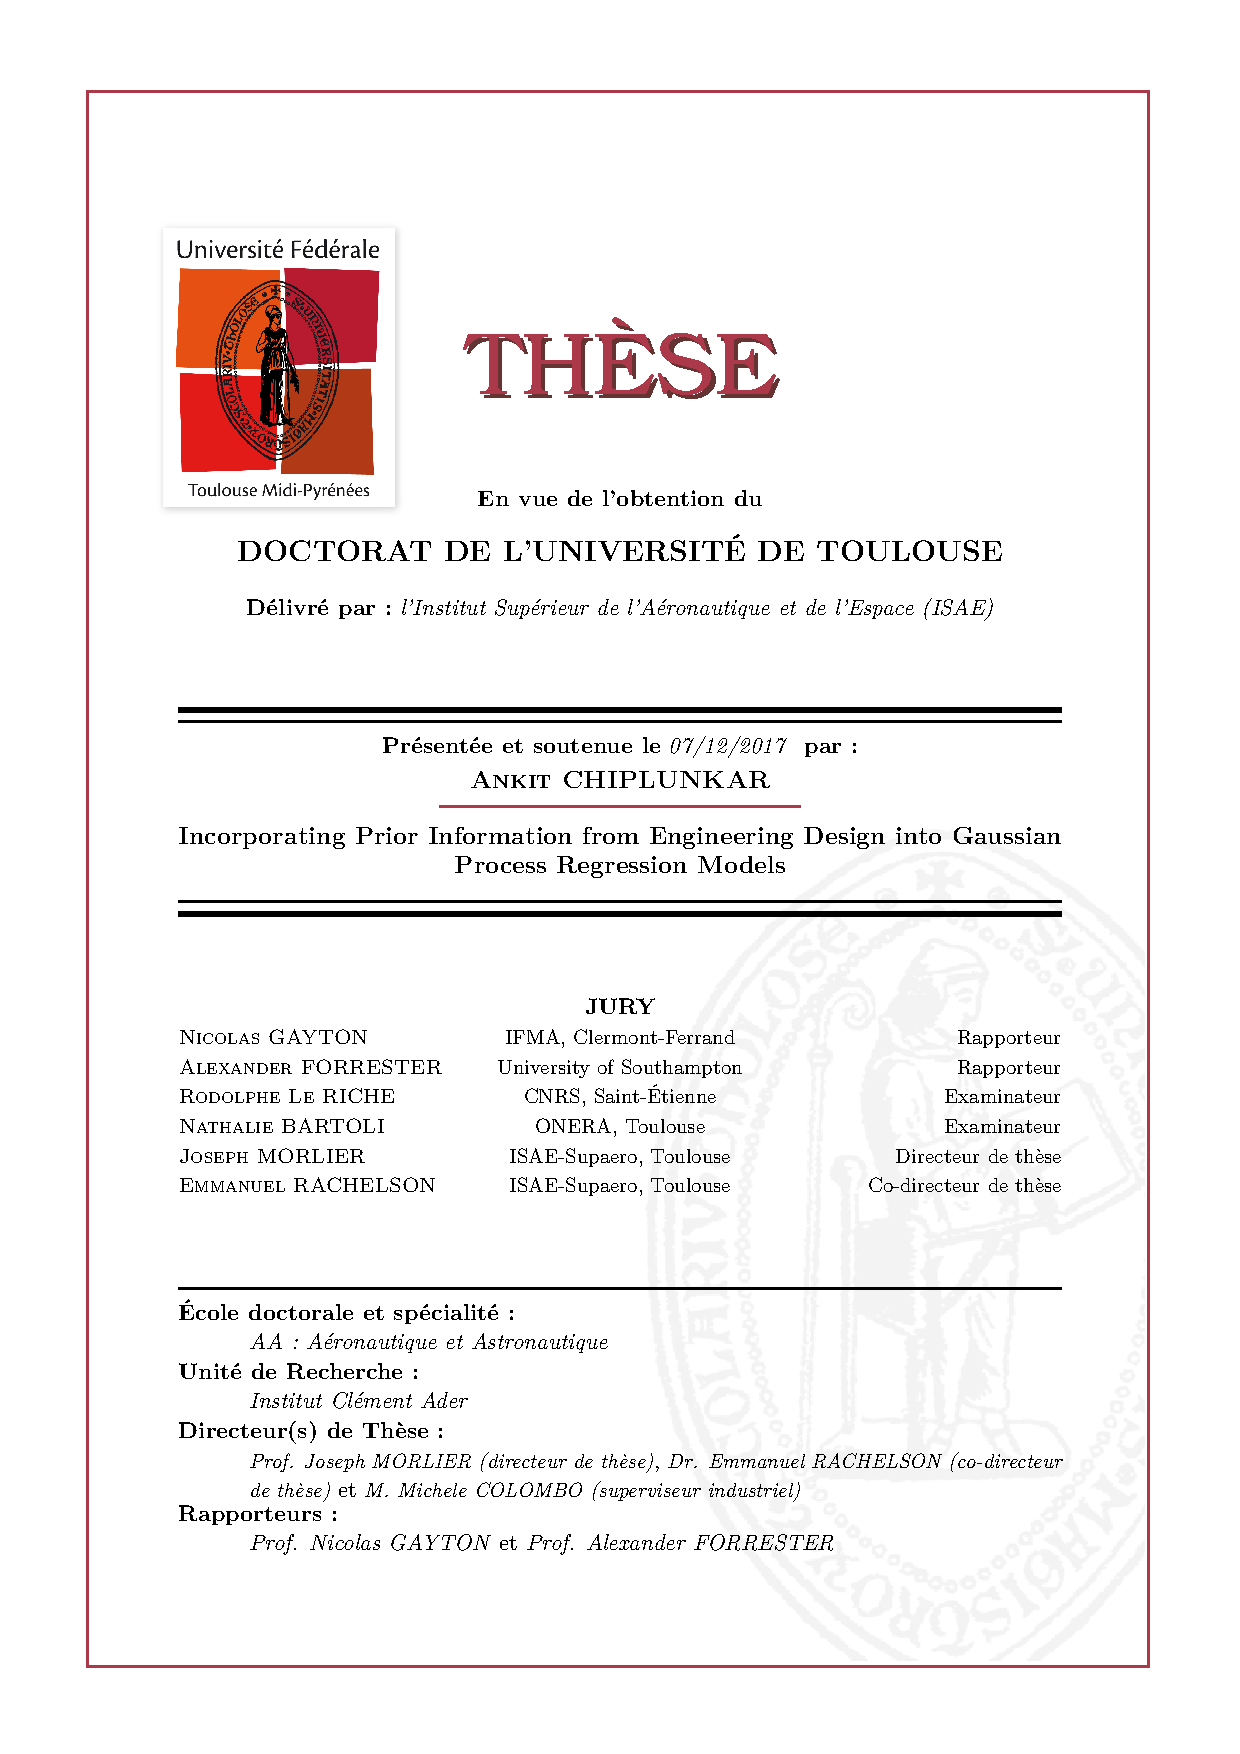
\includepdf[pages={1}]{1-opening/firstPage_ankitThesis.pdf}

%%%%%%%%%%%%%%%%%%%%%%%%%%%%%
%%% Acknowledgements %%%
%%%%%%%%%%%%%%%%%%%%%%%%%%%%%

\frontmatter
\chapter*{Acknowledgements}
I would, first of all, extend my gratitude to Dr. Nicolas Gayton and Dr. Alexander Forrester for accepting to review this thesis and Dr. Nathalie Bartoli and Dr. Rodolphe Le Riche for agreeing to be part of the jury. 

This research work being a CIFRE thesis gave me the opportunity to work, both in an academic environment (ISAE Toulouse) and in a company (Airbus Operations S.A.S.). On the academic side, I would like to thank my tutors Dr. Joseph Morlier and  Dr. Emmanuel Rachelson. They both patiently listened to my wacky ideas and nudged me into more productive directions. They have the capability to understand and explain concepts from their lowest principles, a quality which I admire and would like to replicate.  

At Airbus, I am really indebted to my industrial supervisor Michele Colombo, who took part in developing the wacky ideas and attempting to make them work, working with him has been the exact opposite of a stereotypical Ph.D experience (context: \url{http://phdcomics.com/}). I would also like to thank Sebastien Blanc for encouraging and helping me integrate into the French-speaking environment. He believed in my capabilities and let me apply algorithms in the intensive flight-test campaign. 

I thank the whole EGLRM team at Airbus, my colleagues during the plateau, members of the V\&V IPT, and researchers at the ICA lab. I have really enjoyed my conversations with Hitul Dhoru, Simon Trapier, Alex Calder, Elisa Bosco and Sebastian Delord. 

As always, I am forever grateful to my family for their love and understanding, my father for his inspiration, my mother for her unconditional love, my brother for being my bro and my wife for tolerating my sense of humor. 

While all the above people have shaped me in the last 3 years by their presence, I have learned a lot virtually from the blogs of Vitalik Buterin, tweets of Naval Ravikant and books of Yuval Noah Harari, I extend my thanks to them as well. 

%%%%%%%%%%%%%%%%%%%%%%%%%%%%%
%%% Quotation %%%
%%%%%%%%%%%%%%%%%%%%%%%%%%%%%
%% ----------------------------------------------------------------
% The "Quote Page"
\pagestyle{empty}  % No headers or footers for the following pages

\null\vfill
% Now comes the "Quote", written in italics
\textit{``Stand on the shoulders of giants''}

\begin{flushright}
Google Scholar Motto
\end{flushright}

\vfill\vfill\vfill\vfill\vfill\vfill\null
\clearpage  % Funny Quote page ended, start a new page
%% ----------------------------------------------------------------

%%%%%%%%%%%%%%%%
%%% Abstract %%%
%%%%%%%%%%%%%%%%

% Include the abstract
\cleardoublepage
%\begin{vcenterpage}
\noindent\rule[2pt]{\textwidth}{0.5pt}
%\begin{center}
%{\large\textbf{Title in english\\}}
%\end{center}
{\large\textbf{Abstract ---}}
Due to the high cost of performing experiments on physical systems, models become an efficient means to designing them. Traditionally, these models were built by research institutes, by iteratively performing experiments in a controlled environment. A more cost effective method of building models is by using machine learning algorithms, which infer patterns from data and can be used to perform interpolation and extrapolation. In this thesis, we propose to build better GP regression models by integrating the prior knowledge of Aircraft design with experimental data. 

We demonstrate how to incorporate the prior information by mainly changing the covariance functions of the GP. Prior information in terms of smoothness, linearity, differentiability, etc. can be easily encoded using simple covariance functions. Using the spectral mixture kernels we demonstrate how to build models for structural dynamic experiments and automatically identify dynamic parameters such as modal frequency. To the best of our knowledge, such a method has not been used in earlier literature to identify the modal parameters. We then use the change-point kernel to identify onset of non-linearity, and use a neural network kernel to interpolate shock in transonic regime. For each application we compare the proposed model with the state of the art model and demonstrate the cost or performance gains achieved. 

Similarly, relationships between multiple outputs can be learned or enforced by manipulating the covariance functions. We first demonstrate how the prior information of simulation model can be incorporated to perform extrapolation of experimental data. We then incorporate the physical laws of flight-mechanics into GP regression to identify flight loads. For both the use-cases, we first validate the methodology on a synthetic dataset and then demonstrate the gains on a flight-test dataset.

A limitation of GPs is that they scale very poorly with data, there are two main methods of scaling GPs. The first substitutes the dataset using a reduced set of inducing inputs, while the second distributes the dataset into smaller batches. We demonstrate the scaling capabilities achieved, by building a GP model for interpolating pressures on millions of nodes in a CFD mesh. To the best of our knowledge this scale of GP model has not been created before for interpolating aerodynamic pressures. A similar surrogate model was used in a recent Airbus flight test campaign to compare the pressures predicted from high-fidelity CFD computations to the pressures measured real time on the wing. We then demonstrate how to scale up multiple output GPs to large number of data points, using both approximations. The proposed approach was then validated on a synthetic dataset and on a flight test dataset.

{\large\textbf{Keywords:}}
    Gaussian Process, Flight-Mechanics, Aircraft design, Structural Dynamics, Shock Interpolation.
\\
\noindent\rule[2pt]{\textwidth}{0.5pt}

\pagebreak

\noindent\rule[2pt]{\textwidth}{0.5pt}

{\large\textbf{Résumé ---}}
En raison du coût élevé des essais sur les systèmes physiques, les modèles numériques deviennent un moyen préférentiel pour les concevoir. Traditionnellement, ces modèles numériques ont été construits par des instituts de recherche dans une façon itérative, en effectuant des expériences dans un environnement contrôlé. Une méthode plus efficiente de construction de modèles consiste à utiliser des algorithmes d'apprentissage statistique, qui déduisent des modèles à partir de données et peuvent être utilisés pour interpoler et extrapoler. Dans cette thèse, nous proposons de construire de meilleurs modèles de régression du GP en intégrant la connaissance préalable de la conception d'aéronef avec des données expérimentales.

Nous démontrons comment intégrer l'information préalable en modifiant principalement les fonctions de covariance du GP. En utilisant les noyaux de mélange spectral, nous démontrons comment construire des modèles pour des expériences dynamiques structurelles et identifier automatiquement des paramètres dynamiques comme la fréquence modale. Nous utilisons ensuite le noyau de `change-point' pour identifier l'apparition des non-linéarités et utiliser un noyau de réseau neuronal pour interpoler le choc dans le régime transsonique. Pour chaque application, nous comparons le modèle proposé avec le modèle d'état de l'art et démontrons les gains de coût ou de performance obtenus.


De même, les relations entre plusieurs sorties peuvent être apprises ou imposées en manipulant les fonctions de covariance. Nous démontrons d'abord comment l'information préalable du modèle de simulation peut être incorporée pour effectuer une extrapolation des données expérimentales. Nous incorporons ensuite les lois physiques de la mécanique de vol dans la régression du GP pour identifier les charges de vol. Pour les deux cas d'utilisation, nous validons d'abord la méthodologie sur un ensemble de données synthétiques, puis démontrons les gains sur des données d'essai en vol.

Une limitation des GPs est que effectuer une régression pour un grand nombre de données devient coûteux très vite, deux méthodes pour étendre des GPs existent. La première 'Sparse GPs' utilise un ensemble des points inductifs pour réduire le coût de calcul de la matrice de précision. La seconde est appelée `Distributed GP ' elle divise l'ensemble de données en sous-ensembles plus petits, en divisant le modèle en plusieurs lots. Nous démontrons l’avantage de, construit un modèle GP pour interpoler les pressions sur des millions de nœuds dans un maillage CFD. À notre meilleure connaissance, une modèle du GP de cette taille n'a jamais été créée pour l'interpolation des pressions. Un modèle de substitution similaire a été utilisé pour une récente campagne de d'essai en vol d'Airbus. Nous démontrons ensuite comment étendre les MTGP à un grand nombre de sorties, à la fois en utilisant une approximation `Sparse GP’ et une approximation de `Distributed GP ‘. L'approche proposée a ensuite été validée sur un ensemble de données synthétiques et sur un ensemble de données d'essai en vol.

{\large\textbf{Mots clés :}}
    Processus gaussien, Mécanique de vol, Conception d'aéronefs, Dynamique structurale, Interpolation de choc.
\\
\noindent\rule[2pt]{\textwidth}{0.5pt}





%\begin{center}
%  Institut Cl\'ement Ader, 3 Rue Caroline Aigle\\
%  Toulouse, France
%\end{center}
%\end{vcenterpage}

%%% Local Variables: 
%%% mode: latex
%%% TeX-master: "../phdthesis"
%%% End: 


%%%%%%%%%%%%%%%%
%%% Page numbering and other stuff %%%
%%%%%%%%%%%%%%%%

\clearpage
\tableofcontents

\clearpage
\listoffigures

\clearpage
\lstlistoflistings

\clearpage
%\chapter*{Nomenclature}
%\addstarredchapter{List of 1-symbols}
\markright{List of 1-symbols}
\printnomenclature%[1in]
% Remember to use italic fonts for foreign words
%\begin{acronym}[CP-OFDMX] % Specify the longest acronym in order to set the first column width
% Math identities
\nomenclature[0-nota]{$a$}{Scalar $a$, written in lowercase}
\nomenclature[0-nota]{$\VEC{a}$}{Vector $\VEC{a}$, written in bold lowercase}
\nomenclature[0-nota]{$\VEC{a}^T$}{Transpose of vector $\VEC{a}$}
\nomenclature[0-nota]{$\myMatrix{A}$}{Matrix $\myMatrix{A}$, written in bold uppercase}
\nomenclature[0-nota]{$\mathcal{R}$}{Set of all real numbers}
\nomenclature[0-nota]{$\Pr[a]$}{Probability distribution of $a$}
\nomenclature[0-nota]{$\Pr[a, b]$}{Joint probability distribution of $a$ and $b$}
\nomenclature[0-nota]{$\Pr[a \mid b]$}{Conditional probability distribution of $a$ given $b$}
\nomenclature[0-nota]{$\mathcal{N}[\mu, \sigma^2]$}{Scalar Gaussian distribution}
\nomenclature[0-nota]{$\mathcal{N}[\VEC{\mu}, \myMatrix{\Sigma}]$}{Multivariate Gaussian Distribution}
\nomenclature[0-nota]{$GP[m(x), k(x, x')]$}{Gaussian Process}

% Math Symbols
\nomenclature[1-sym]{$x_i$}{$i^{th}$ observational input point}
\nomenclature[1-sym]{$\myMatrix{X}$}{Full training input dataset}
\nomenclature[1-sym]{$\myMatrix{X^M}$}{Set of inducing points}
\nomenclature[1-sym]{$\myMatrix{X^j}$}{Full set of inputs for the $j^{th}$ output for MTGP}
\nomenclature[1-sym]{$\myMatrix{X_{joint}}$}{Joint input dataset for MTGP}
\nomenclature[1-sym]{$x_*$}{Single test input point}
\nomenclature[1-sym]{$\myMatrix{x_*}$}{Full test input dataset}
\nomenclature[1-sym]{$y_i$}{$i^{th}$ observational output point}
\nomenclature[1-sym]{$\VEC{y}$}{Full training output dataset}
\nomenclature[1-sym]{$\VEC{y}^j$}{Full set of outputs for the $j^{th}$ output for MTGP}
\nomenclature[1-sym]{$\VEC{y_{joint}}$}{Joint output dataset for MTGP}

% symbols for parameters
\nomenclature[1-sym]{$w$}{Parameters of functions}
\nomenclature[1-sym]{$\VEC{\theta}$}{Vector of hyper-parameters}
\nomenclature[1-sym]{$\theta_{lengthScale}$}{Length scale hyper-parameter}
\nomenclature[1-sym]{$\theta_{amplitude}$}{Amplitude hyper-parameter}
\nomenclature[1-sym]{$\theta_{intensity}$}{Intensity hyper-parameter for $k_{CP}$}
\nomenclature[1-sym]{$\theta_{changeLocation}$}{Change location hyper-parameter}

% list of symbols
\nomenclature[1-sym]{$\epsilon$}{Independent white noise}
\nomenclature[1-sym]{$\delta$}{Dirac-delta function}
\nomenclature[1-sym]{$\sigma_n^2$}{Variance of the white noise}
\nomenclature[1-sym]{$d$}{Distance between two input points}
\nomenclature[1-sym]{$\tau$}{Time lag between two points}
\nomenclature[1-sym]{$\nu$}{Degrees of freedom of student distribution}
\nomenclature[1-sym]{$\lambda_i$}{$i^{th}$ modal frequency}
\nomenclature[1-sym]{$A_i$}{$i^{th}$ mode shape}
\nomenclature[1-sym]{$\omega_i$}{$i^{th}$ spatial coordinate of the aerodynamic node}
\nomenclature[1-sym]{$\Omega$}{Full spatial coordinates of the aerodynamic mesh}
\nomenclature[1-sym]{$p_i$}{Pressure at the $i^{th}$ aerodynamic node}
\nomenclature[1-sym]{$\myMatrix{P}$}{Full Pressure data for the aerodynamic mesh}
\nomenclature[1-sym]{$b$}{Wing span}
\nomenclature[1-sym]{$T_z$}{Shear Load on the wing}
\nomenclature[1-sym]{$M_x$}{Bending moment on the wing}
\nomenclature[1-sym]{$\eta_{edge}$}{Wing span at the edge of the wing}
\nomenclature[1-sym]{$\eta_{root}$}{Wing span at the root of the wing}

% Number of things
\nomenclature[1-sym]{$N$}{Number of points in training dataset}
\nomenclature[1-sym]{$N_*$}{Number of points in test dataset}
\nomenclature[1-sym]{$N_{experts}$}{Number of experts in distributed GP}
\nomenclature[1-sym]{$N_{hyp}$}{Number of hyper-parameters}
\nomenclature[1-sym]{$M$}{Number of inducing points}
\nomenclature[1-sym]{$P$}{Number of points in an expert}
\nomenclature[1-sym]{$D_{inputs}$}{Number of dimensions in input data}
\nomenclature[1-sym]{$D_{outputs}$}{Number of dimensions in the output data}
\nomenclature[1-sym]{$Q$}{Number of Gaussians in a SM kernel}
\nomenclature[1-sym]{$N_{nodes}$}{Number of nodes in aerodynamic mesh}
\nomenclature[1-sym]{$N_{experiments}$}{Number of experiments}
\nomenclature[1-sym]{$N_{j}$}{Number of points in the $j^{th}$ output for MTGP}
\nomenclature[1-sym]{$N_{joint}$}{Total number of points for MTGP}

\nomenclature[1-sym]{$f$}{Function mapping transformation from $x$ to $y$}
\nomenclature[1-sym]{$f_{pressure}$}{Pressure function mapping transformation from $\omega_i$ to $p_i$}
\nomenclature[1-sym]{$\phi(x)$}{Basis functions}
\nomenclature[1-sym]{$\mathcal{D}_i$}{$i^{th}$ Data-set}

\nomenclature[1-sym]{$\myMatrix{I_N}$}{Identity matrix of size $N$}
\nomenclature[1-sym]{$\myMatrix{\Sigma_{Prior}}$}{Covariance matrix of prior over parameters}
\nomenclature[1-sym]{$\myMatrix{K(X_1, X_2)}$}{Gram matrix between $\myMatrix{X_1}$ and $\myMatrix{X_2}$}
\nomenclature[1-sym]{$\myMatrix{K_{Nystrom}}$}{Gram matrix using Nystr\"{o}m approximation}
\nomenclature[1-sym]{$\myMatrix{K_{FITC}}$}{Gram matrix using FITC approximation}
\nomenclature[1-sym]{$\myMatrix{K_{lower}}$}{Lower Cholesky decomposition of Gram matrix}
\nomenclature[1-sym]{$\myMatrix{K_{outputs}}$}{Covariance matrix between output dimensions}

\nomenclature[1-sym]{$diag(\myMatrix{K})$}{Diagonal of the matrix}
\nomenclature[1-sym]{$\myMatrix{M}$}{Mass matrix}
\nomenclature[1-sym]{$\myMatrix{C}$}{Damping matrix}
\nomenclature[1-sym]{$\myMatrix{K_{stiffness}}$}{Stiffness matrix}
\nomenclature[1-sym]{$\myMatrix{H}$}{Low-rank matrix}

\nomenclature[1-sym]{$\mu$}{Mean value of a Gaussian Distribution}
\nomenclature[1-sym]{$m(x)$}{Mean function a GP}
\nomenclature[1-sym]{$k(x, x')$}{Covariance function a GP}
\nomenclature[1-sym]{$k^{\delta}$}{Covariance function of the difference between multi-fidelity GPs}
\nomenclature[1-sym]{$m^{(i)}(x)$}{Predicted mean of the $i^{th}$ expert}
\nomenclature[1-sym]{$\sigma^{(i)}(x)$}{Predicted covariance of the $i^{th}$ expert}
\nomenclature[1-sym]{$\mathbf{E}[x]$}{Expectation of the random variable x}
\nomenclature[1-sym]{$Cov[x, x']$}{Covariance between two random variables}

% Acronyms
\nomenclature[2-abb]{$ARD$}{Automatic Relevance Determination}
\nomenclature[2-abb]{$ANOVA$}{Analysis Of Variance}
\nomenclature[2-abb]{$BCM$}{Bayesian Committee Machine}
\nomenclature[2-abb]{$BIC$}{Bayesian Information Criterion}
\nomenclature[2-abb]{$CFD$}{Computational Fluid Dynamics}
\nomenclature[2-abb]{$CP$}{Change-Point}
\nomenclature[2-abb]{$CRM$}{Common Research Model}
\nomenclature[2-abb]{$CV$}{Cross Validation}
\nomenclature[2-abb]{$EMA$}{Experimental Modal Analysis}
\nomenclature[2-abb]{$FEM$}{Finite Element Method}
\nomenclature[2-abb]{$FITC$}{Fully Independent Training Conditional}
\nomenclature[2-abb]{$FTF$}{Flap Track Fairing}
\nomenclature[2-abb]{$GP$}{Gaussian Process}
\nomenclature[2-abb]{$gPOE$}{generalized Product Of Experts}
\nomenclature[2-abb]{$HCT$}{Heritage Court Tower}
\nomenclature[2-abb]{$IT$}{Information Technology}
\nomenclature[2-abb]{$LOO$}{Leave One Out}
\nomenclature[2-abb]{$MDO$}{Multi Disciplinary Optimization}
\nomenclature[2-abb]{$MDOF$}{Multi Degree Of Freedom}
\nomenclature[2-abb]{$NExT$}{Natural Excitation Technique}
\nomenclature[2-abb]{$OMA$}{Operational Modal Analysis}
\nomenclature[2-abb]{$PCA$}{Principal Component Analysis}
\nomenclature[2-abb]{$POE$}{Product Of Experts}
\nomenclature[2-abb]{$POD$}{Proper Orthogonal Decomposition}
\nomenclature[2-abb]{$PSD$}{Positive Semi Definite}
\nomenclature[2-abb]{$RANS$}{Reynolds Averaged  Navier-Stokes}
\nomenclature[2-abb]{$rBCM$}{robust Bayesian Committee Machine}
\nomenclature[2-abb]{$RFP$}{Rational Fractional Polynomial}
\nomenclature[2-abb]{$RMSE$}{Root Mean Square Error}
\nomenclature[2-abb]{$ROM$}{Reduced Order Models}
\nomenclature[2-abb]{$SE$}{Standard Exponential}
\nomenclature[2-abb]{$SVD$}{Singular Value Decomposition}



%\end{acronym}

% To cite an acronym in the text : \ac{ASK}
% To cite an acronym in the text without footnote : \acs{ASK}

%%% Local Variables: 
%%% mode: latex
%%% TeX-master: "../phdthesis"
%%% End: 



%%%%%%%%%%%%%%%%%%%%%%%%%%%%%%%%%%%%%%%%%%%%
%%% Content of the report and references %%%
%%%%%%%%%%%%%%%%%%%%%%%%%%%%%%%%%%%%%%%%%%%%

\mainmatter
\pagestyle{fancy}

\cleardoublepage

\part{Introduction}\label{partIntroduction}
\chapter{Context}
\markboth{Context}{Context}
\label{chapIntroduction}
%\minitoc

\marginnote{\textsl{Machine learning}}[1cm]
In the past decade due to the boom in Information Technology (IT) companies, more investment has gone into developing both computational infrastructure and methods. One of the ubiquitous methods developed due to this investment is that of Machine Learning. Learning algorithms look for patterns in data to learn from them and make decisions. They are used in web search, optimization, spam filtering, ad placement, stock trading, healthcare, manufacturing, space exploration, particle physics, security, and lot more. The speed and adaptability of learning methods are changing everything around us one algorithm at a time \cite{domingos2015master}. The World Economic Forum, Davos 2016 \cite{schwab2016fourth} has dubbed this as the fourth industrial revolution; first was steam powered, second was electrically powered, third was IT powered, fourth will be powered by artificial intelligence algorithms.

\marginnote{\textsl{Aircraft design}}[1cm]
In comparison aircraft design is almost a century old field, the first successful flight being by the Wright brothers in 1903 \cite{wright1934we}. Currently, the design of an aircraft is a highly-iterative optimization process. Based on the initial target objectives and general trends, aircraft designers define the objectives for domain specific departments (eg. aerodynamics design or structural design). These objectives further trickle down to more dedicated teams and tasks (eg airfoil design or fuselage design). This gives rise to a huge Multi-Disciplinary Optimization (MDO) problem. Teams come up with individual constraints, they iterate around their domains, interact with neighboring domains and negotiate overlapping constraints. Teams negotiate and solidify individual objectives and constraints to find the optimized design for an aircraft. An optimized design as close to the initial target objectives, an optimized design taking into account the sparse infrastructure, human and economic limitations. This is a massive MDO problem spanning almost a decade, costing billions and involving thousands of people. 

\begin{figure}[!ht]
\label{figPhasesOfAircraftDesign}
  \centering
  
    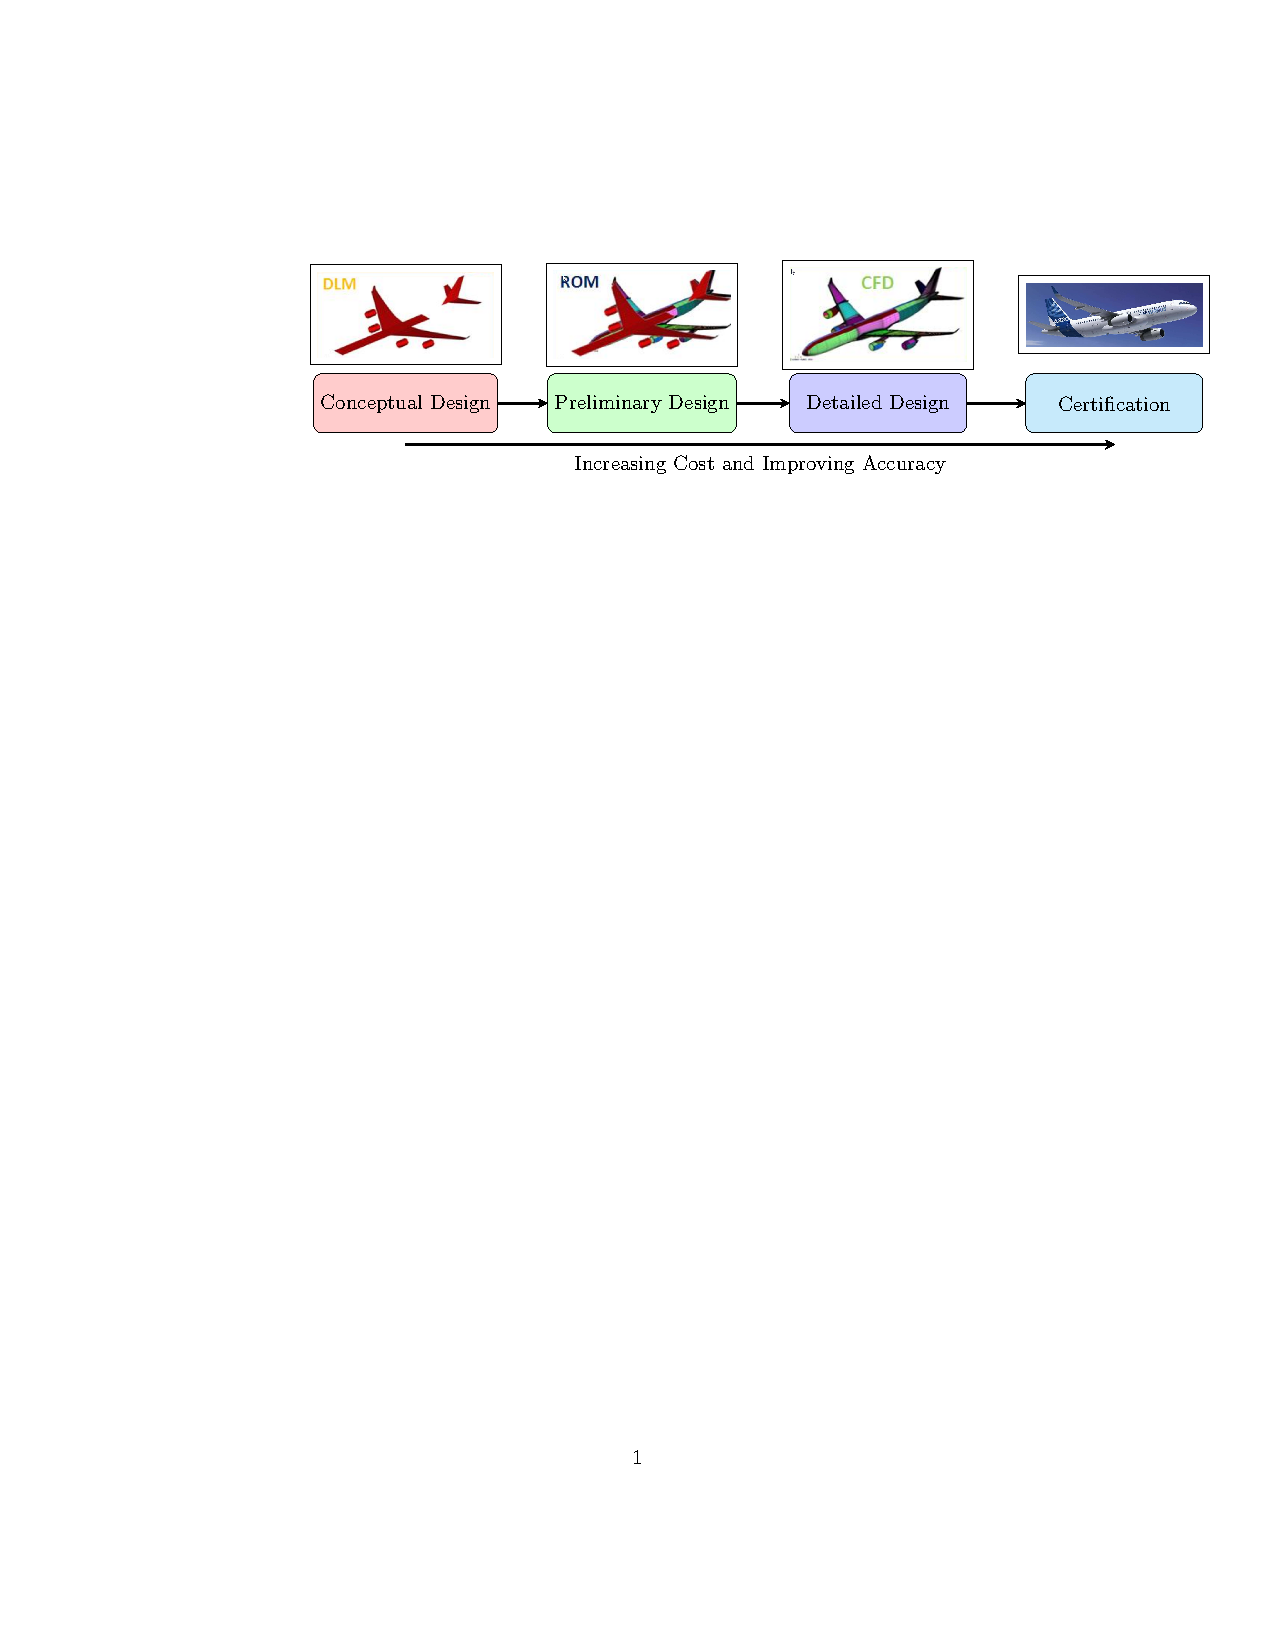
\includegraphics[clip, trim=4.5cm 19cm 0.5cm 4cm,width=0.95\textwidth]
    {images/part1/aircraftDesignCycleFlowChart}
  
  \caption{Phases of an aircraft design cycle}
\end{figure}

\section{Aircraft design cycle}\label{secSircraftDesignCycle}
\marginnote{\textsl{Design phases}}[1cm]
To simplify this process an aircraft design is broken down into several design phases (figure \ref{figPhasesOfAircraftDesign}). Each phase requires an ever increasing amount of predictions and fidelity. Preliminary design phase requires a few low-fidelity design trade-offs between major disciplines. Whereas, during detailed design phase, intensive intra-disciplinary and inter-disciplinary optimization's take place. Finally, during the flight-test and certification phase capability to predict real-time can provide significant gains in reducing the flight-test phase. These analyses cover large parts of flight envelope and require high-fidelity predictions. Hence the capability to accurately and quickly predict is an integral part of an aircraft design cycle \cite{raymer2012aircraft}. 

\marginnote{\textsl{Need for Speed}}[1cm]
In the last decade high-fidelity, physics based, mathematical simulations have become central to designing an aircraft. However, high-fidelity simulations are computationally expensive, this is the case for several Computational Fluid Dynamics (CFD) and Finite Element Method (FEM) based solvers. Due to this high cost high-fidelity simulations are launched only for a few carefully chosen design configurations. This results in inefficient exploration of the the design space and thus a non-optimal design. A common strategy to speed up simulations is by reducing the physical complexity of the model to make quick predictions. As an example linear potential flows (simpler aerodynamic model), or coarser FEM meshes (simpler structural model) are regularly used during the preliminary design phase \cite{cummings2015applied}. While this is an acceptable practice during the preliminary design phase, during the detailed design phase physical complexity is needed to find a robust optimum design point \cite{raymer2012aircraft}.

\marginnote{\textsl{Need for accuracy}}[1cm]
Instead of approximating physical complexity, surrogate models\footnote{Surrogate models, learning algorithms and machine learning models will be used interchangeably throughout this manuscript} simplify mathematical complexity \cite{verveld2016reduced}. Surrogate models learn patterns between the input and output dataset and then are used to make predictions on the desired point. This property is very useful in quickly exploring the design space and finding a robust design point \cite{forrester2008engineering}. Moreover, surrogate models are commonly passed across disciplines to perform inter-disciplinary optimizations. For example, a loads department would prefer running a quick surrogate model over the costly CFD model while performing the load's loop.  

\marginnote{\textsl{Deduction vs Induction}}[1cm]
The main difference between the engineering design and surrogate modeling can be explained by the difference between deduction and induction \cite{domingos2012few} (figure \ref{fig:engineeringDesignVsSurrogateModelling}). Engineering design is deduction: where a very general formula is applied to a particular case (figure \ref{figDeduction}). The basics of Newtonian physics, when applied to a particular aircraft geometry, give inertial loads. The basics of aerodynamics, when applied to a particular set of aircraft geometry and aircraft states, give out aerodynamic pressures. Engineering design takes global rules and applies them to local configurations. Whereas, surrogate modeling is induction: it looks at local features and data, tries to find similarity measures between them and gives a global formula for the process (figure \ref{figInduction}). For example, an algorithm to detect faces in images will look at several images with and without faces, learn a facial pattern and make predictions on new images \cite{marszalek2007semantic}. We here see a possible complementary relationship between engineering design and machine learning; where engineering design needs models to generate data, machine learning needs data to generate models.

\begin{figure}[!ht]\label{fig:engineeringDesignVsSurrogateModelling}
  \centering
  \subfigure[Engineering design - Deduction: The figure shows an application of a general rule to a particular case.]
  {
    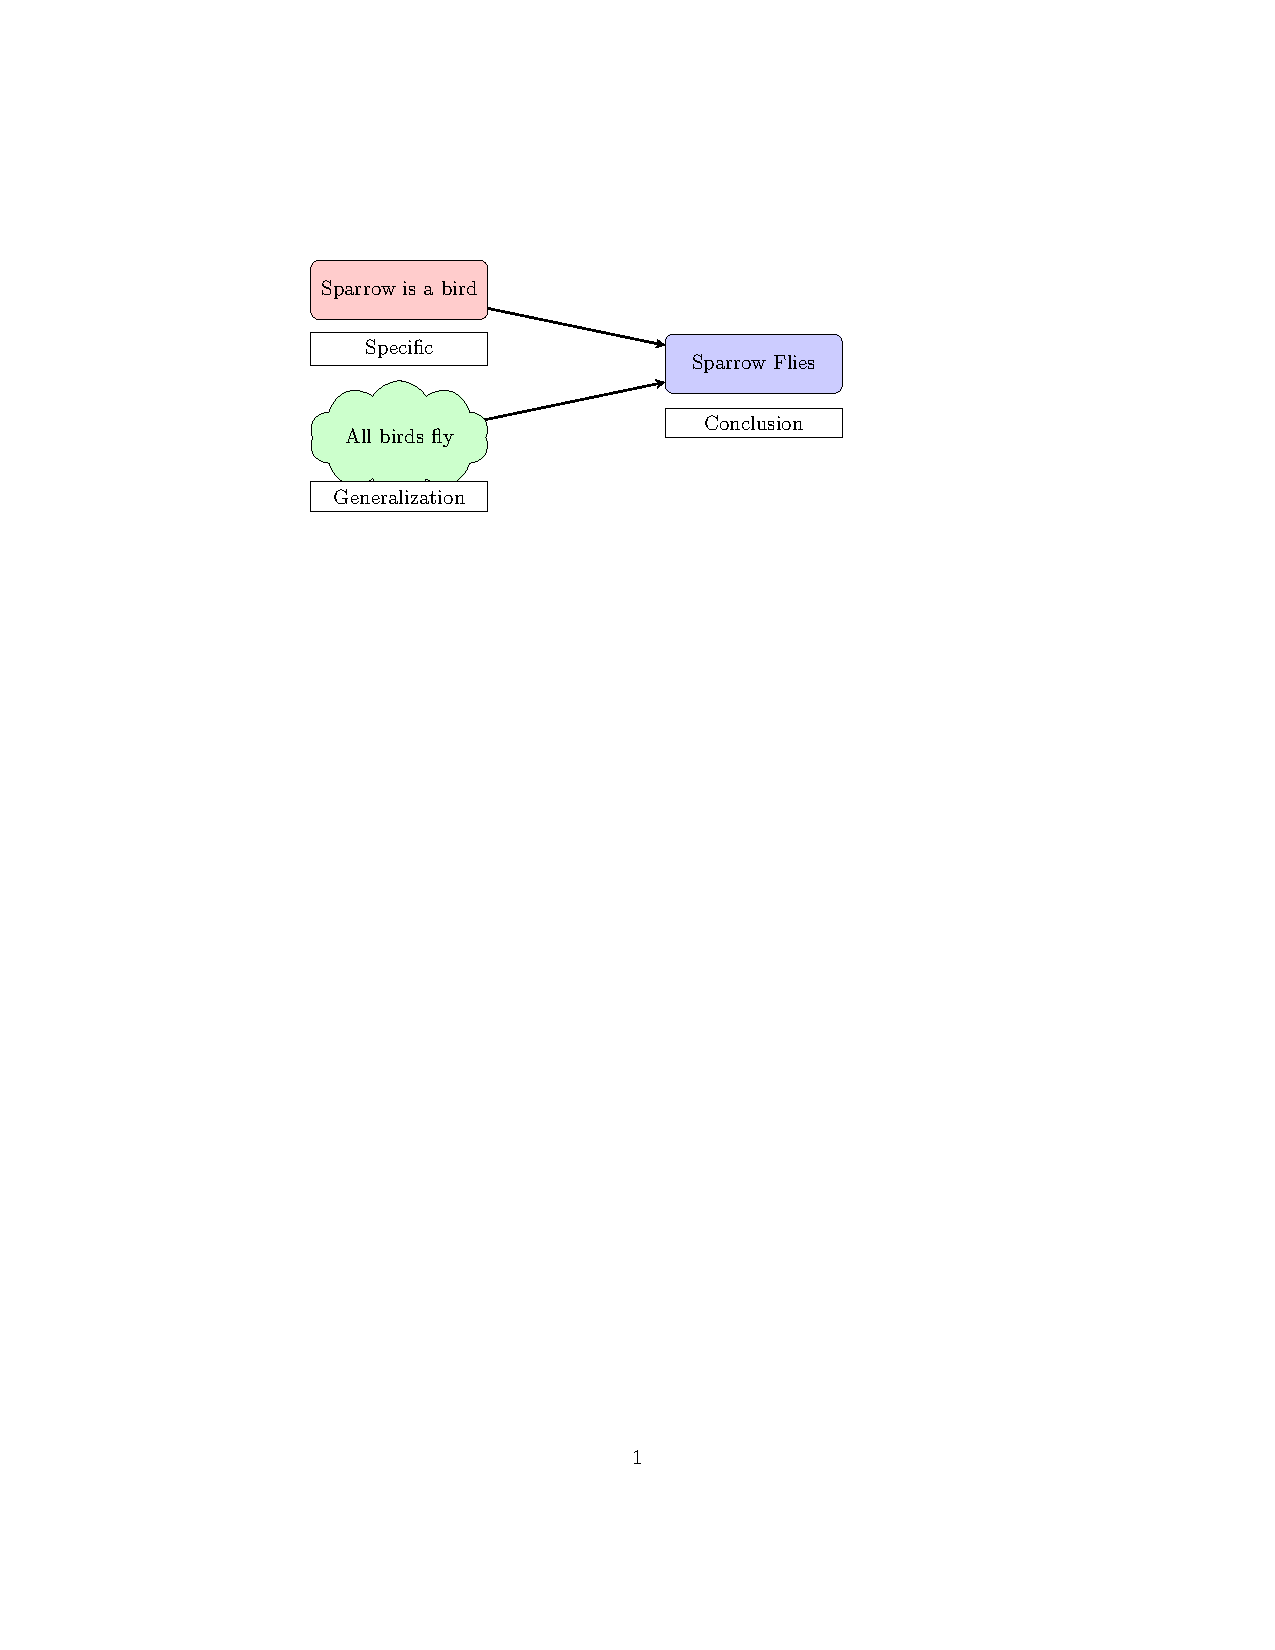
\includegraphics[clip, trim=4.5cm 19cm 4.5cm 4cm,width=0.45\textwidth]
    {images/part1/deduction}
    \label{figDeduction}
  }\quad
  \subfigure[Surrogate modelling - Induction: The figure shows how multiple examples can be used to infer underlying rules or patterns that govern the system.]
  {
    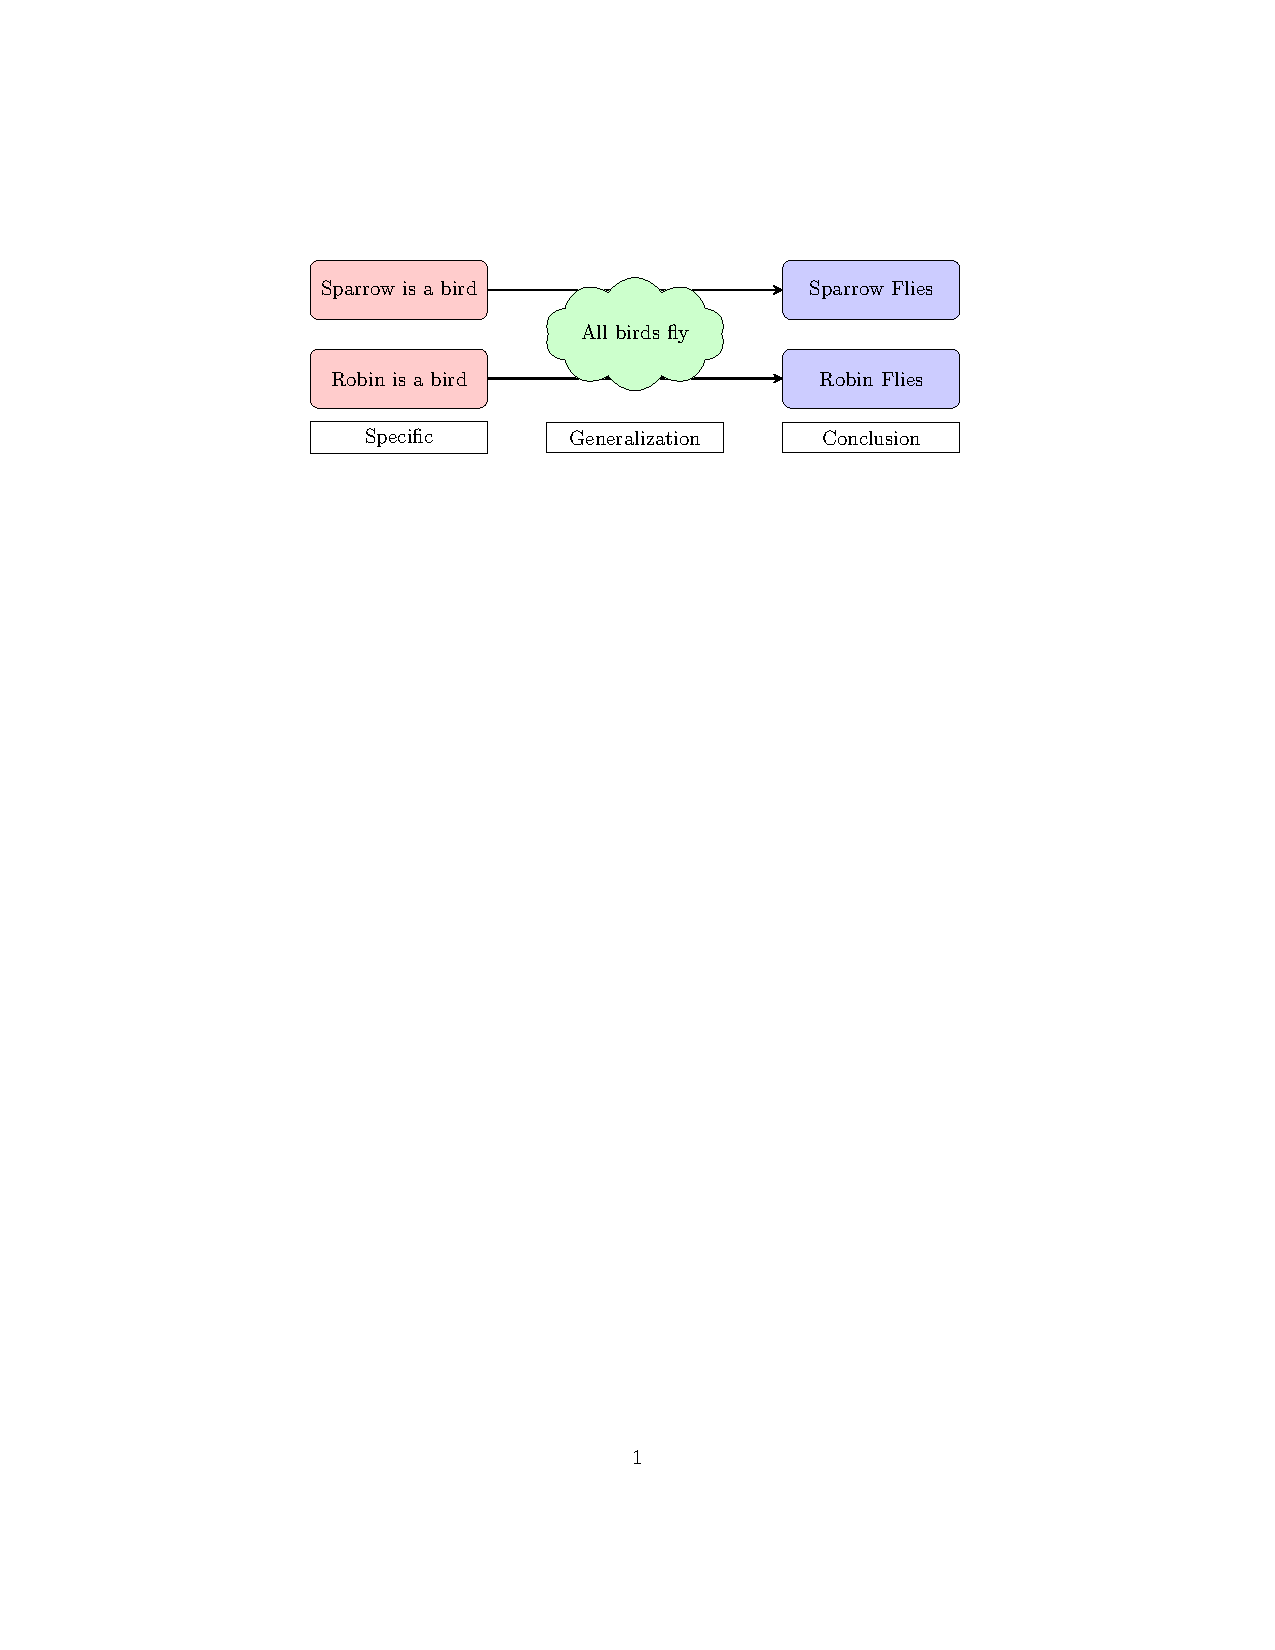
\includegraphics[clip, trim=4.5cm 20cm 4.5cm 4cm,width=0.45\textwidth]
    {images/part1/induction}
    \label{figInduction}
  }\quad
  \caption{Induction vs Deduction}
\end{figure}

\marginnote{\textsl{Developing faster models}}[1cm]
Since models are an integral part of any engineering design, model building in aircraft engineering was traditionally outsourced to research institutes. Researchers perform iterative experiments in a controlled environment and discover patterns between the physics of the system. For example, it took 200 years to iteratively develop the Gas law \footnote{$Pressure \times Volume \propto numberOfMoles \times Temperature$}, Boyle's law in 1600's found the relation between Pressure and Volume, Charle's Law in 1787 discovered the relationship between Volume and Temperature, while Gay-Lussac's Law in 1809 discovered the relationship between Pressure and Temperature \cite{clapeyron1834memoire}. This is a rigorous and time-consuming method of developing models. Machine learning is a much more elegant method of building models. Using data and few basic assumptions, automatic models can be built between desired inputs and outputs. For example, while the first model of a neural network was proposed in 1950's \cite{kleene1951representation}, neural networks are today used daily for tasks such as tagging cat photos on facebook and converting speech to text\footnote{I wrote a fourth of this thesis using a text to speech software}. In this thesis, we wish to automatically build models for aircraft design tasks primarily to be used during the detailed design phase and certification phase. 


\section{Machine Learning}\label{secMachineLearning}
\marginnote{\textsl{Components of learning}}[1cm]
The core objective of learning algorithms is to find a transformation function between the inputs and outputs. There are three main components in a learning algorithm:
\begin{enumerate}
\item \textbf{Representation}: A learning algorithm starts with a family of functions. For example, a linear model is a family of linear functions, a trigonometric model defines a family of trigonometric functions. If an algorithm is not able to represent the actual function in its family of functions, it will find the closest function in its hypothesis space\footnote{The term family of functions, hypothesis space and representation will be used interchangeably throughout this manuscript}.
\item \textbf{Evaluation}: Some measure is needed to distinguish a good function from a bad function in the chosen hypothesis space. This measure is termed as evaluation; one example is the least squares error commonly used in many learning algorithms. 
\item \textbf{Optimization}: Finally, the algorithm iteratively searches in its hypothesis space to find the best possible function explaining the data. The choice of optimizer defines the speed of learning and is also important if there are multiple minima in the evaluation criteria.
\end{enumerate}

\marginnote{\textsl{Bias vs Variance}}[1cm]
Surrogate models suffer from the bias vs variance trade-off (figure \ref{figBiasVsVariance}), formalized by `Wolpert' in his famous "no free lunch theorem" \cite{wolpert1997no}. The constituent functions in a hypothesis space represent the bias or assumptions of the learning algorithm (eg. linear functions for linear regression). In the absence of sufficient assumptions, the family of functions in the search space becomes very large which leads to high variance or over-fitting in the surrogate model (figure \ref{subFigpredictionPoly15}). On the contrary, wrong bias means that the true transformation function ($f$) does not exist in the hypothesis space. In this case, the learning algorithm finds the function closest to $f$ in its hypothesis space and leads to under-fitting (figure \ref{subFigpredictionPoly6}).

\begin{figure}[!ht]
  \centering
    \subfigure[{High-bias and low variance}]
  {
        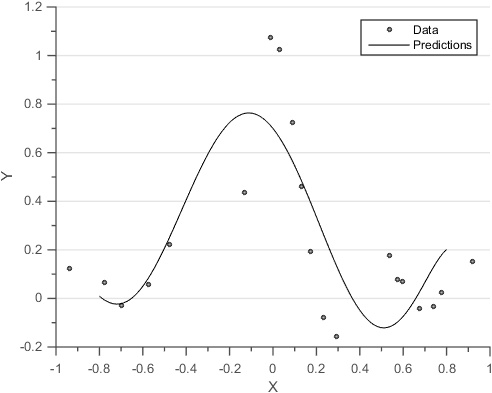
\includegraphics[width=0.29\textwidth]
        {images/part1/predictionPoly6}
        \label{subFigpredictionPoly6}
  }\quad
\subfigure[{Low bias and High variance}]
  {
        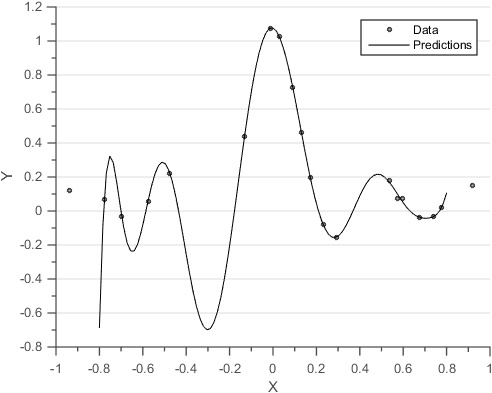
\includegraphics[width=0.29\textwidth]
        {images/part1/predictionPoly15}
        \label{subFigpredictionPoly15}
  }\quad
  \subfigure[{Bias replaced with lots of data}]
  {
        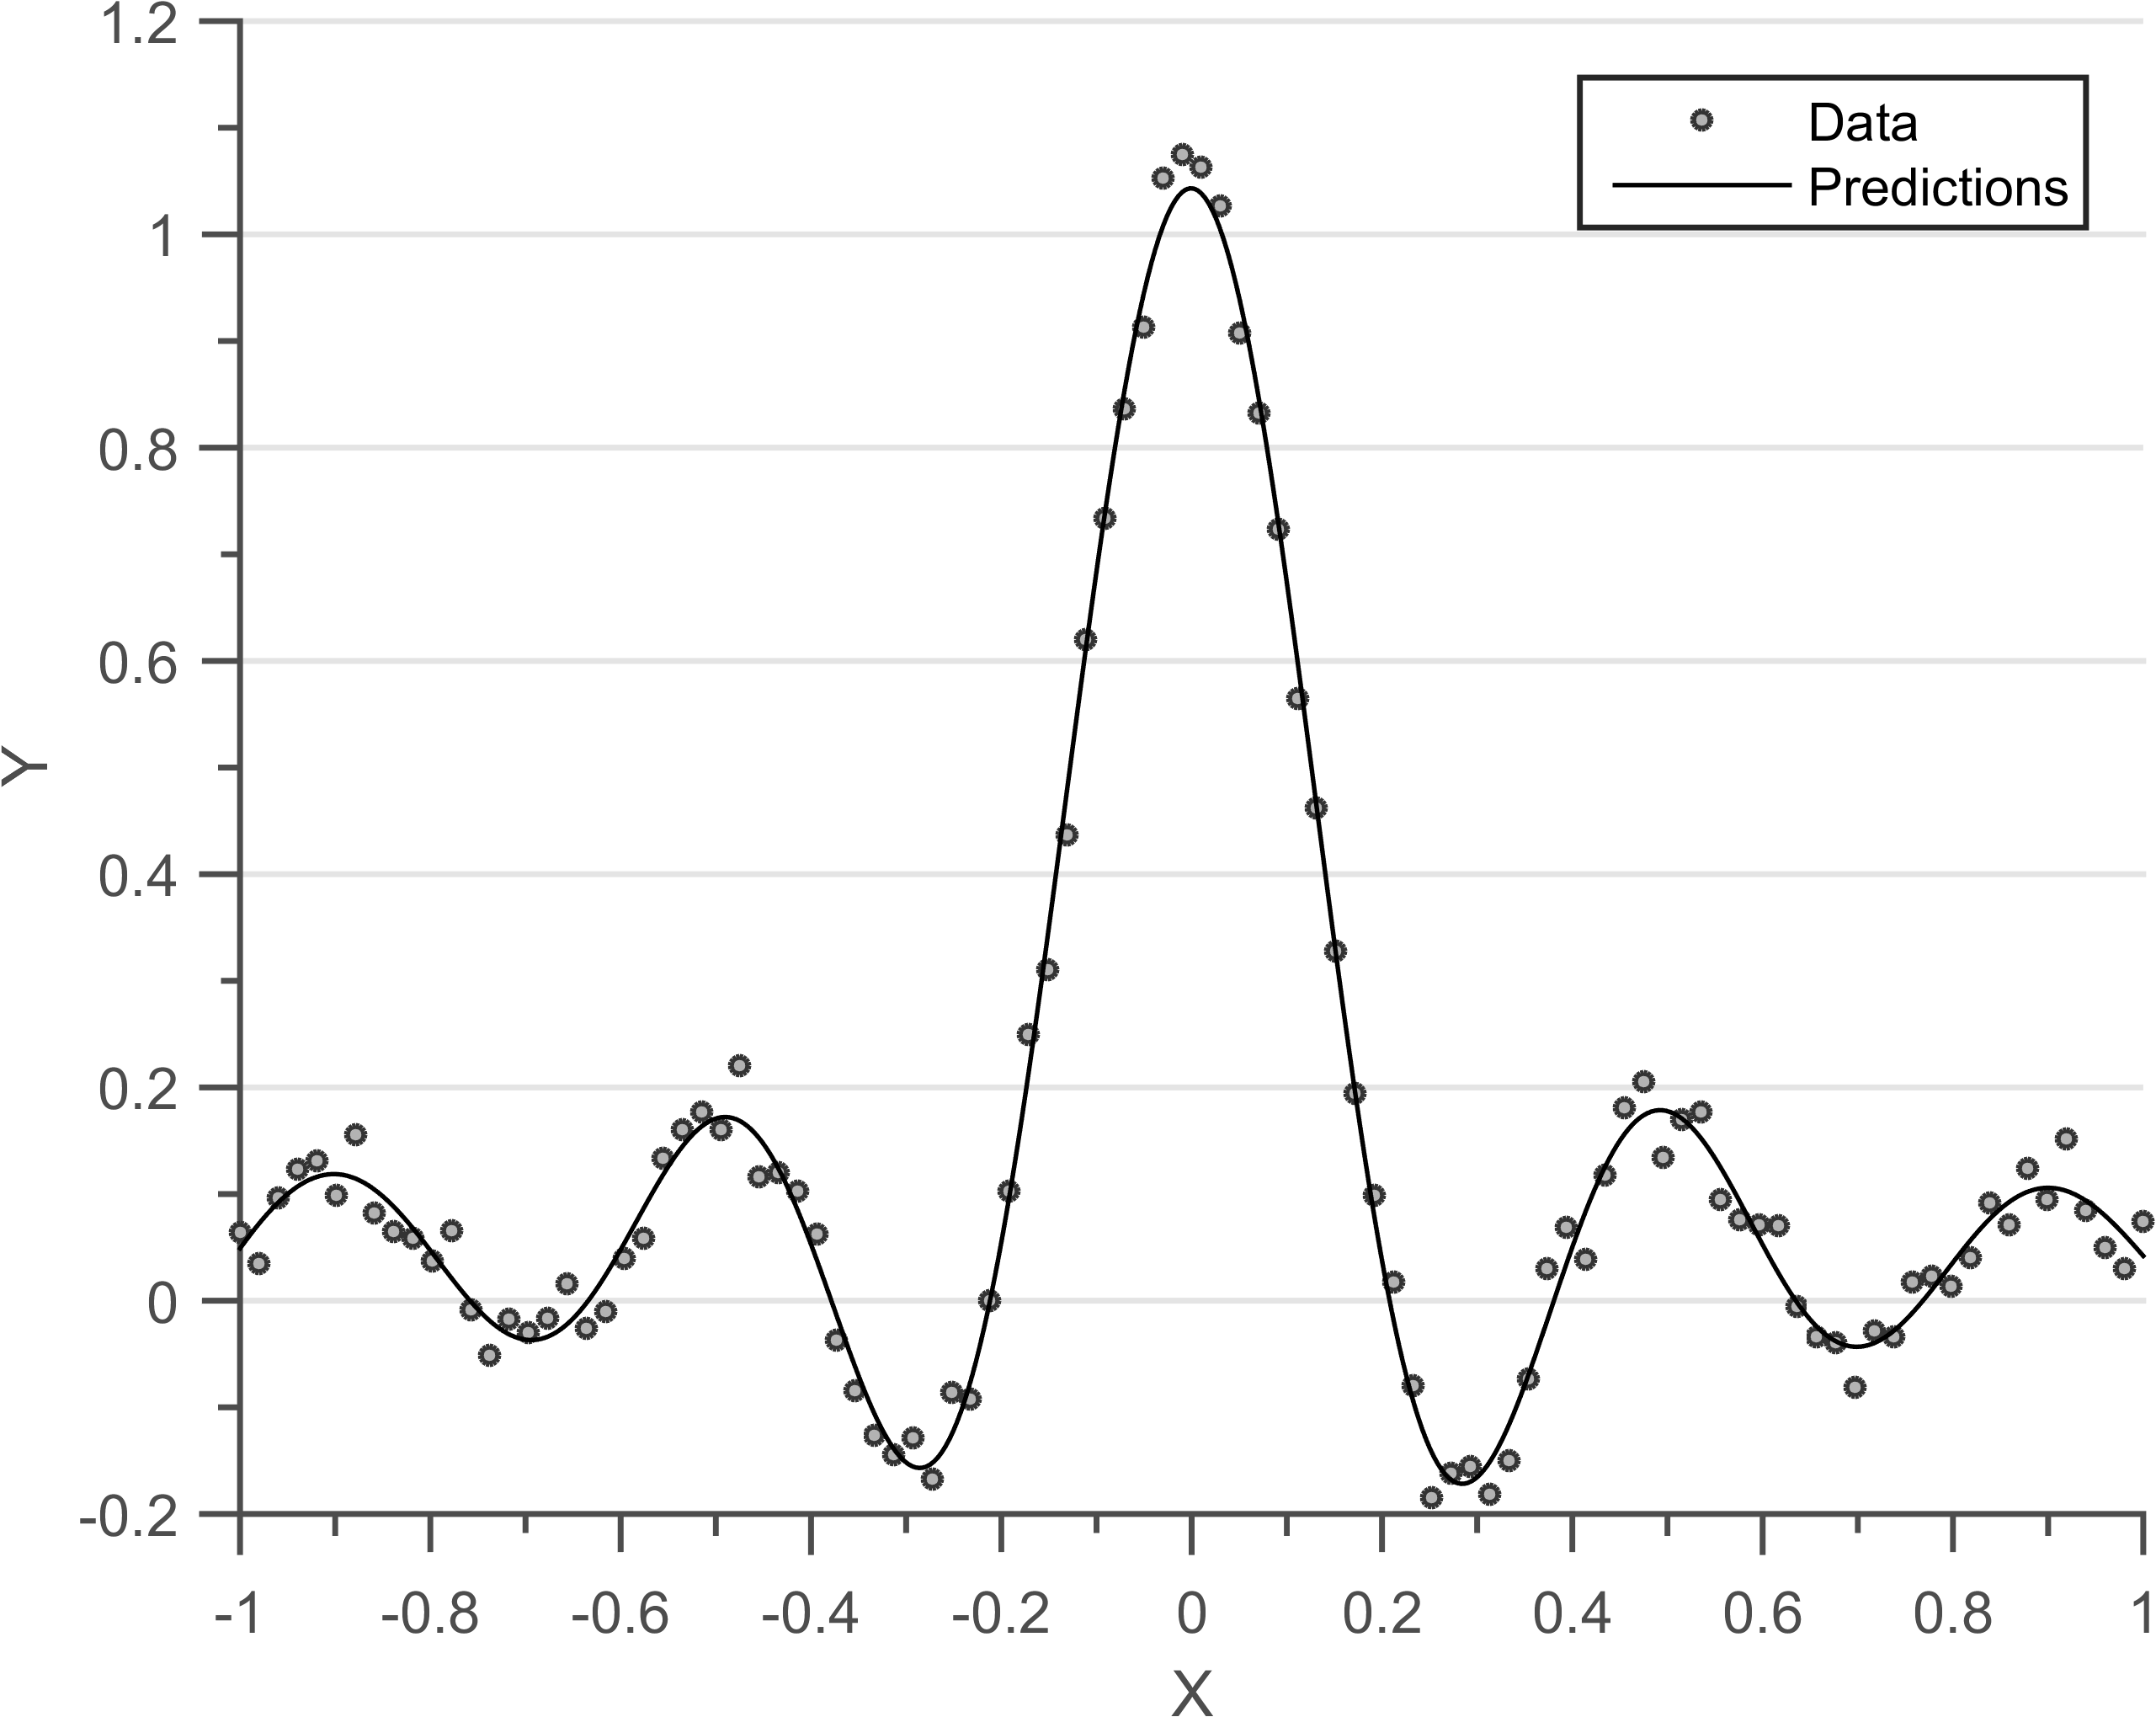
\includegraphics[width=0.29\textwidth]
        {images/part1/posteriorSEInitialAtI100}
        \label{subFigposteriorSEInitialAtI100}
  }\quad
       \caption{Bias vs Variance trade-off}
       \label{figBiasVsVariance}
\end{figure}



\marginnote{\textsl{Soft and hard constraints}}[1cm]
One method to overcome this trade-off is by using lots and lots of data. Data acts as a hard constraint for learning algorithm, imagine a family of all possible continuous 2-dimensional functions in the range of $x \in [-1, 1]$ and $y \in [-1, 1]$. What will happen, given an observation $(x = 0, y = 0)$. All the functions that do not pass through this point will be eliminated, the new data point has basically reduced the possible family of functions. Whereas, bias acts as soft constraint, we can use the bias of linearity or smoothness to reduce our hypothesis space. Therefore, both bias and data help in reducing the hypothesis space\footnote{Bias can also be looked upon as distilled knowledge or patterns gained after interpreting huge amounts data}. Given access to more and more data, we can progressively reduce the bias in learning models thereby relying more on true evidence. This is also the main concept behind deep learning, where several layers of neural networks define a very large hypothesis space \cite{Goodfellow-et-al-2016, lecun2015deep}. 

Unfortunately in aircraft design, generating a huge amount of accurate data is a costly exercise, for example a high fidelity CFD simulation runs for weeks \cite{murthy2014computational, jameson2012computational} and a flight-test campaign costs millions of euros \cite{fox2004test}. On another hand due to centuries of research and tinkering, we have a treasure trove of prior information about the physical systems. We propose to build better machine learning models by integrating the time-tested prior knowledge of physical systems with experimental data. 

\begin{mdframed}[hidealllines=true,backgroundcolor=blue!20]
\marginnote{\textsl{Contribution}}[1cm]
The main contribution of this thesis is to provide a framework on how to combine the prior knowledge from a physical system and add it to a learning algorithm. A model generated from merging of the two methodologies will be both consistent with the physics of the system and be quicker to evaluate. We integrate three types of prior knowledge by answering the following questions:
\begin{enumerate}
\item \textbf{Pattern}: How to add \textit{apriori} information of a pattern in a learning algorithm? For example, given that shock is a discontinuous change in pressure, how to predict the position of shock on an airfoil (part \ref{partIncorporatePattern}). 
\item \textbf{Relationships}: How to add \textit{apriori} information of relationships between measurements? For example given $Loads = \int Pressures$, how to make a robust loads model when we measure both pressures and loads (chapter \ref{chapAddingEquationsInGP}).
\item \textbf{Simulation model}: How to merge \textit{apriori} information of simulations with experiments? For example, given a simulation model and experimental data how to perform extrapolations on experimental data(chapter \ref{chapMultiTaskExtrapolation}). 
\end{enumerate}

To integrate the prior information we propose to use a Bayesian inference for model building. Bayesian inference is a method of statistical inference in which Bayes theorem is used to update an initial probability (prior) as more and more evidence becomes available the final probability (posterior) gives our estimate. More specifically, we will use the Gaussian Processes (GP) Regression framework which is a subset of the Bayesian Inference algorithms to define prior information of physical systems. But, before deep diving into the details of GP let us have a look at a simple Bayesian Linear Regression algorithm.
\end{mdframed}

\section{Bayesian Linear Regression}\label{secBayesianModelling}
Suppose we have access to a training set of observations (or outputs) $Y = (y(x_{1}); \ldots ; y(x_{i}); \ldots ; y(x_{N}))$, evaluated at a set of known inputs $X = (x_{1}; \ldots ; x_{i}; \ldots; x_{N})$, and we wish to predict $y(x_{*})$ at a test input $x_{*}$. The input and output can be multi-dimensional; $x_{i} \in \mathbb{R}^{D_{inputs}}$ and $y(x_{i}) \in \mathbb{R}^{D_{outputs}}$. The process of learning the transformation function $f$ to make prediction at a new point is called as regression. In the following section we follow formulation for Bayesian Linear Regression provided by \cite{mackay2003information}.

\marginnote{\textsl{Basis functions}}[1cm]
A simple method to perform regression is by assuming a form of the function $f$, then minimizing the error between the true measurements and assumed form to estimate the parameters of $f$. The function is written in terms of basis functions $\phi(x)$. For example when $\phi(x) = \{1, x\}^{T}$ we are performing linear regression, when $\phi(x) = \{1, x, x^{2}, \ldots, x^{L}\}^{T}$ we are performing $L^{th}$ order polynomial regression. We will focus on linear regression in this section and hence $\phi(x) = \{1, x\}^{T}$.

\begin{equation}\label{eqBayesianLinearRegression}
f(x_{i}) = \begin{Bmatrix}
x^{0} & x^{1}
\end{Bmatrix}  \begin{Bmatrix}
w_{0}\\ 
w_{1}
\end{Bmatrix}
\quad \quad y(x_{i}) = f(x_{i}) + \epsilon
\end{equation}

\marginnote{\textsl{Likelihood}}[1cm]
Here, $w$ are the parameters of the function, $w_{0}$ denotes the intercept and $w_{1}$ denotes the slope of the regression model. The measurements are corrupted by independent white noise $\epsilon$, such that the noise is a random variable sampled from a white noise Gaussian with variance $\sigma_{n}^{2}$\footnote{$\Pr[\epsilon] = \mathcal{N}(0, \sigma_{n} = \frac{1}{\sqrt{2\pi\sigma_{n}^{2}}}\exp^{-\frac{\epsilon^{2}}{2\sigma_{n}^{2}}}
$}. The above equations \ref{eqBayesianLinearRegression} can be combined to result in the likelihood $\Pr[Y\mid X, w]$

\begin{equation}\label{eqBayesianLikelihood}
\begin{aligned}
\Pr[Y \mid X, w]  & = \prod \Pr[y_{i}\mid x_{i}, w]\\
                & = \prod \mathcal{N}[x_{i}w , \sigma_{n}^{2}]\\
                & = \mathcal{N}(X^{T} w, \sigma_{n}^{2}I)    
\end{aligned}
\end{equation}

The notation $\Pr[Y \mid X, w]$ symbolizes probability distribution of observations $Y$ at the inputs $X$ given the parameter $w$. The notation $\mathcal{N}[\mu , \Sigma]$ symbolizes a multi-variate Gaussian distribution for mean vector $\mu$ and covariance matrix $\Sigma$. 

\marginnote{\textsl{Prior}}[1cm]
While performing Bayesian inference we specify a prior distribution to encode our assumptions on the parameters before we look at the observations. For this case, we put a zero mean Gaussian prior on our weights.

\begin{equation}\label{eqBayesianPrior}
\Pr[w] = \mathcal{N}(0, \Sigma_{Prior})
\end{equation}

The prior distribution on $w$ induces a prior distribution over functions parametrized by $w$, effectively we are defining family of functions $(\Pr[f(x_{i})] = \mathcal{N}(0, x_{i}^{T}\Sigma_{Prior}x_{i}))$ by placing a prior distribution over $w$. Once we have a prior distribution encoding our beliefs, we use Bayes rule to look at the observations and get a posterior distribution of parameters.

\begin{equation*}
posterior = \frac{likelihood \times prior}{marginal \quad likelihood}
\end{equation*}
\begin{equation}\label{eqBayesRule}
\Pr[w \mid Y, X] = \frac{\Pr[Y \mid X, w] \times \Pr[w]}{\Pr[Y \mid X]}
\end{equation}

\marginnote{\textsl{Marginal Likelihood}}[1cm]
The \textsl{marginal likelihood} is a normalization constant, for more details please refer to section \ref{secHyperParameter}. After, using the equation \ref{eqBayesianLikelihood}, \ref{eqBayesianPrior} and \ref{eqBayesRule} we can get the posterior distribution of weights as:

\begin{equation}\label{eqBayesianPosterior}
\Pr[w \mid Y, X]  = \mathcal{N}\left ( \frac{1}{\sigma_{n}^{2}} A^{-1}X Y , A^{-1} \right )
\end{equation}

Here, $A = \sigma_{n}^{-2}XX^{T} + \Sigma_{Prior}^{-2}$. Thus the posterior distribution for function $f$ at test point $x_{*}$ becomes:

\begin{equation}\label{eqBayesianFunctionalPosterior}
\Pr[f \mid x_{*}, X, y]  = \mathcal{N}\left ( \frac{1}{\sigma_{n}^{2}} x_{*}A^{-1}XY , x_{*}^{T}A^{-1}x_{*} \right )
\end{equation}

\marginnote{\textsl{Posterior}}[1cm]
The mean $\frac{1}{\sigma_{n}^{2}} x_{*}A^{-1}XY$ can be used as a prediction at the test point $x_{*}$, while the variance is a measure of uncertainty for this prediction. We can thus obtain the prediction $f(x_{*})$, using a prior set of beliefs (equation \ref{eqBayesianPrior}) and updating those beliefs using observations. 

\begin{mdframed}[hidealllines=true,backgroundcolor=lightgray!20]
\marginnote{\textsl{Experiment}}[1cm]
Suppose we have a toy dataset $\mathcal{D}_{1} = \{X = [-0.5, 0.33, 0.66], Y = [0, 0.5, 0.5]\}$ and want to find a function that fits this dataset using Bayesian Linear Regression. If we assume a prior distribution of parameter $w$ as defined by equation \ref{eqExperimentalPrior}, then the probability density of $w$ will look like figure \ref{subFigpriorBLR}.

\begin{equation}\label{eqExperimentalPrior}
\Pr \left [\begin{pmatrix}
w_{0}\\ 
w_{1}
\end{pmatrix} \right ] = \mathcal{N}\left [ \begin{pmatrix}
0\\ 
0
\end{pmatrix}, \Sigma_{P} = \begin{bmatrix}
1 & 0\\ 
0 & 1
\end{bmatrix} \right ]
\end{equation}

Using equations \ref{eqExperimentalPrior} and \ref{eqBayesianFunctionalPosterior} we can calculate the posterior distribution for the parameters. For a noise model of $\Pr[\epsilon] = \mathcal{N}(0, (\sigma_{n}=0.1)^2)$ the posterior distribution comes out as the figure \ref{subFigposteriorBLR}

\begin{equation}\label{eqExperimentalPosterior}
\Pr \left [\begin{pmatrix}
w_{0}\\ 
w_{1}
\end{pmatrix} \mid \mathcal{D}_{1}, \Sigma_{P}, \sigma_{n} \right ] = \mathcal{N}\left [ \begin{pmatrix}
0.2576\\ 
0.4584
\end{pmatrix}, \begin{bmatrix}
0.0037 & -0.0022\\ 
-0.0022 & 0.0138
\end{bmatrix} \right ]
\end{equation}

This simple example demonstrates how to estimate the parameters $w_{0}$ and $w_{1}$ using the prior distribution on parameters $w$ and dataset $\mathcal{D}_{1}$. The estimate of the intercept is $w_{0} = 0.2576$ and slope is $w_{1} = 0.4584$ (equation \ref{eqExperimentalPosterior}), we can use this estimate to plot the value of linear function $f(x)$ (figure \ref{subFigpredictionsBLR}). 
\end{mdframed}

\begin{figure}[!ht]
  \centering
    \subfigure[{Contours of probability density for a prior on parameters $w$ as defined by equation \ref{eqExperimentalPrior}}]
  {
        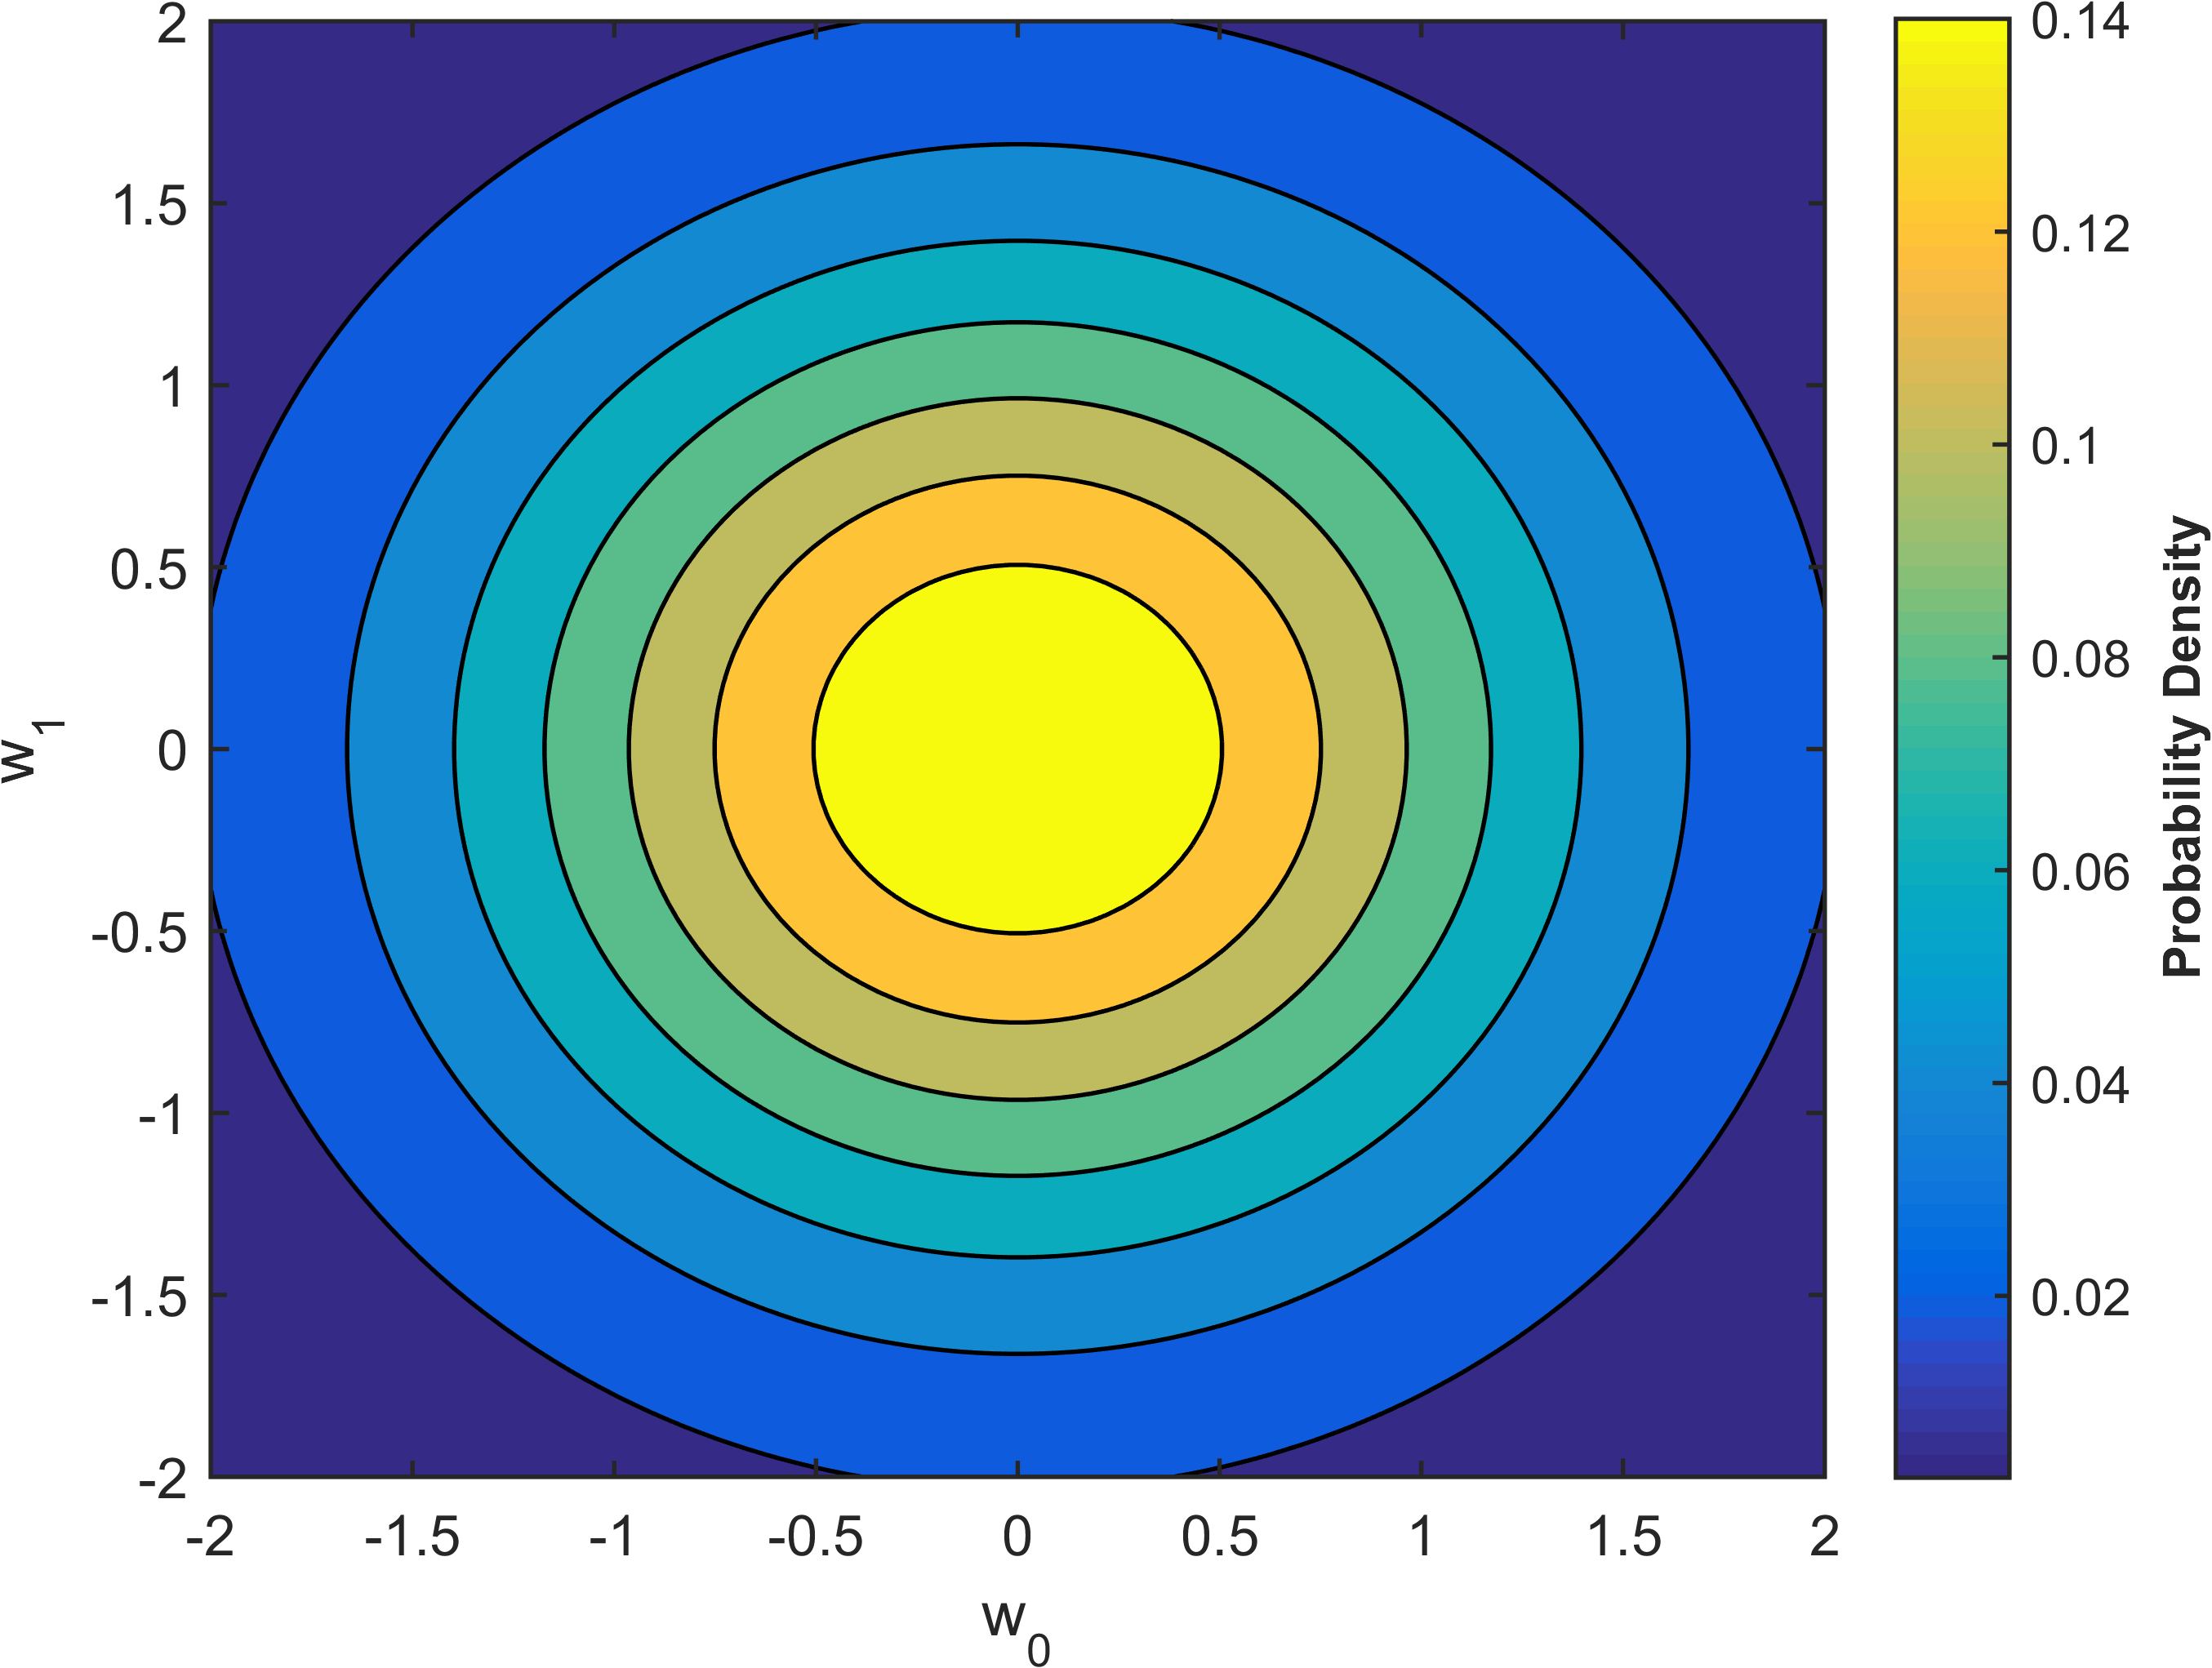
\includegraphics[width=0.29\textwidth]
        {images/part1/priorBLR}
        \label{subFigpriorBLR}
  }\quad
\subfigure[{Contours of probability density for posterior distribution of parameters $w$ using equations \ref{eqExperimentalPrior} and \ref{eqBayesianPosterior}. The predicted intercept is $0.2576$ and the predicted slope is $0.4584$}]
  {
        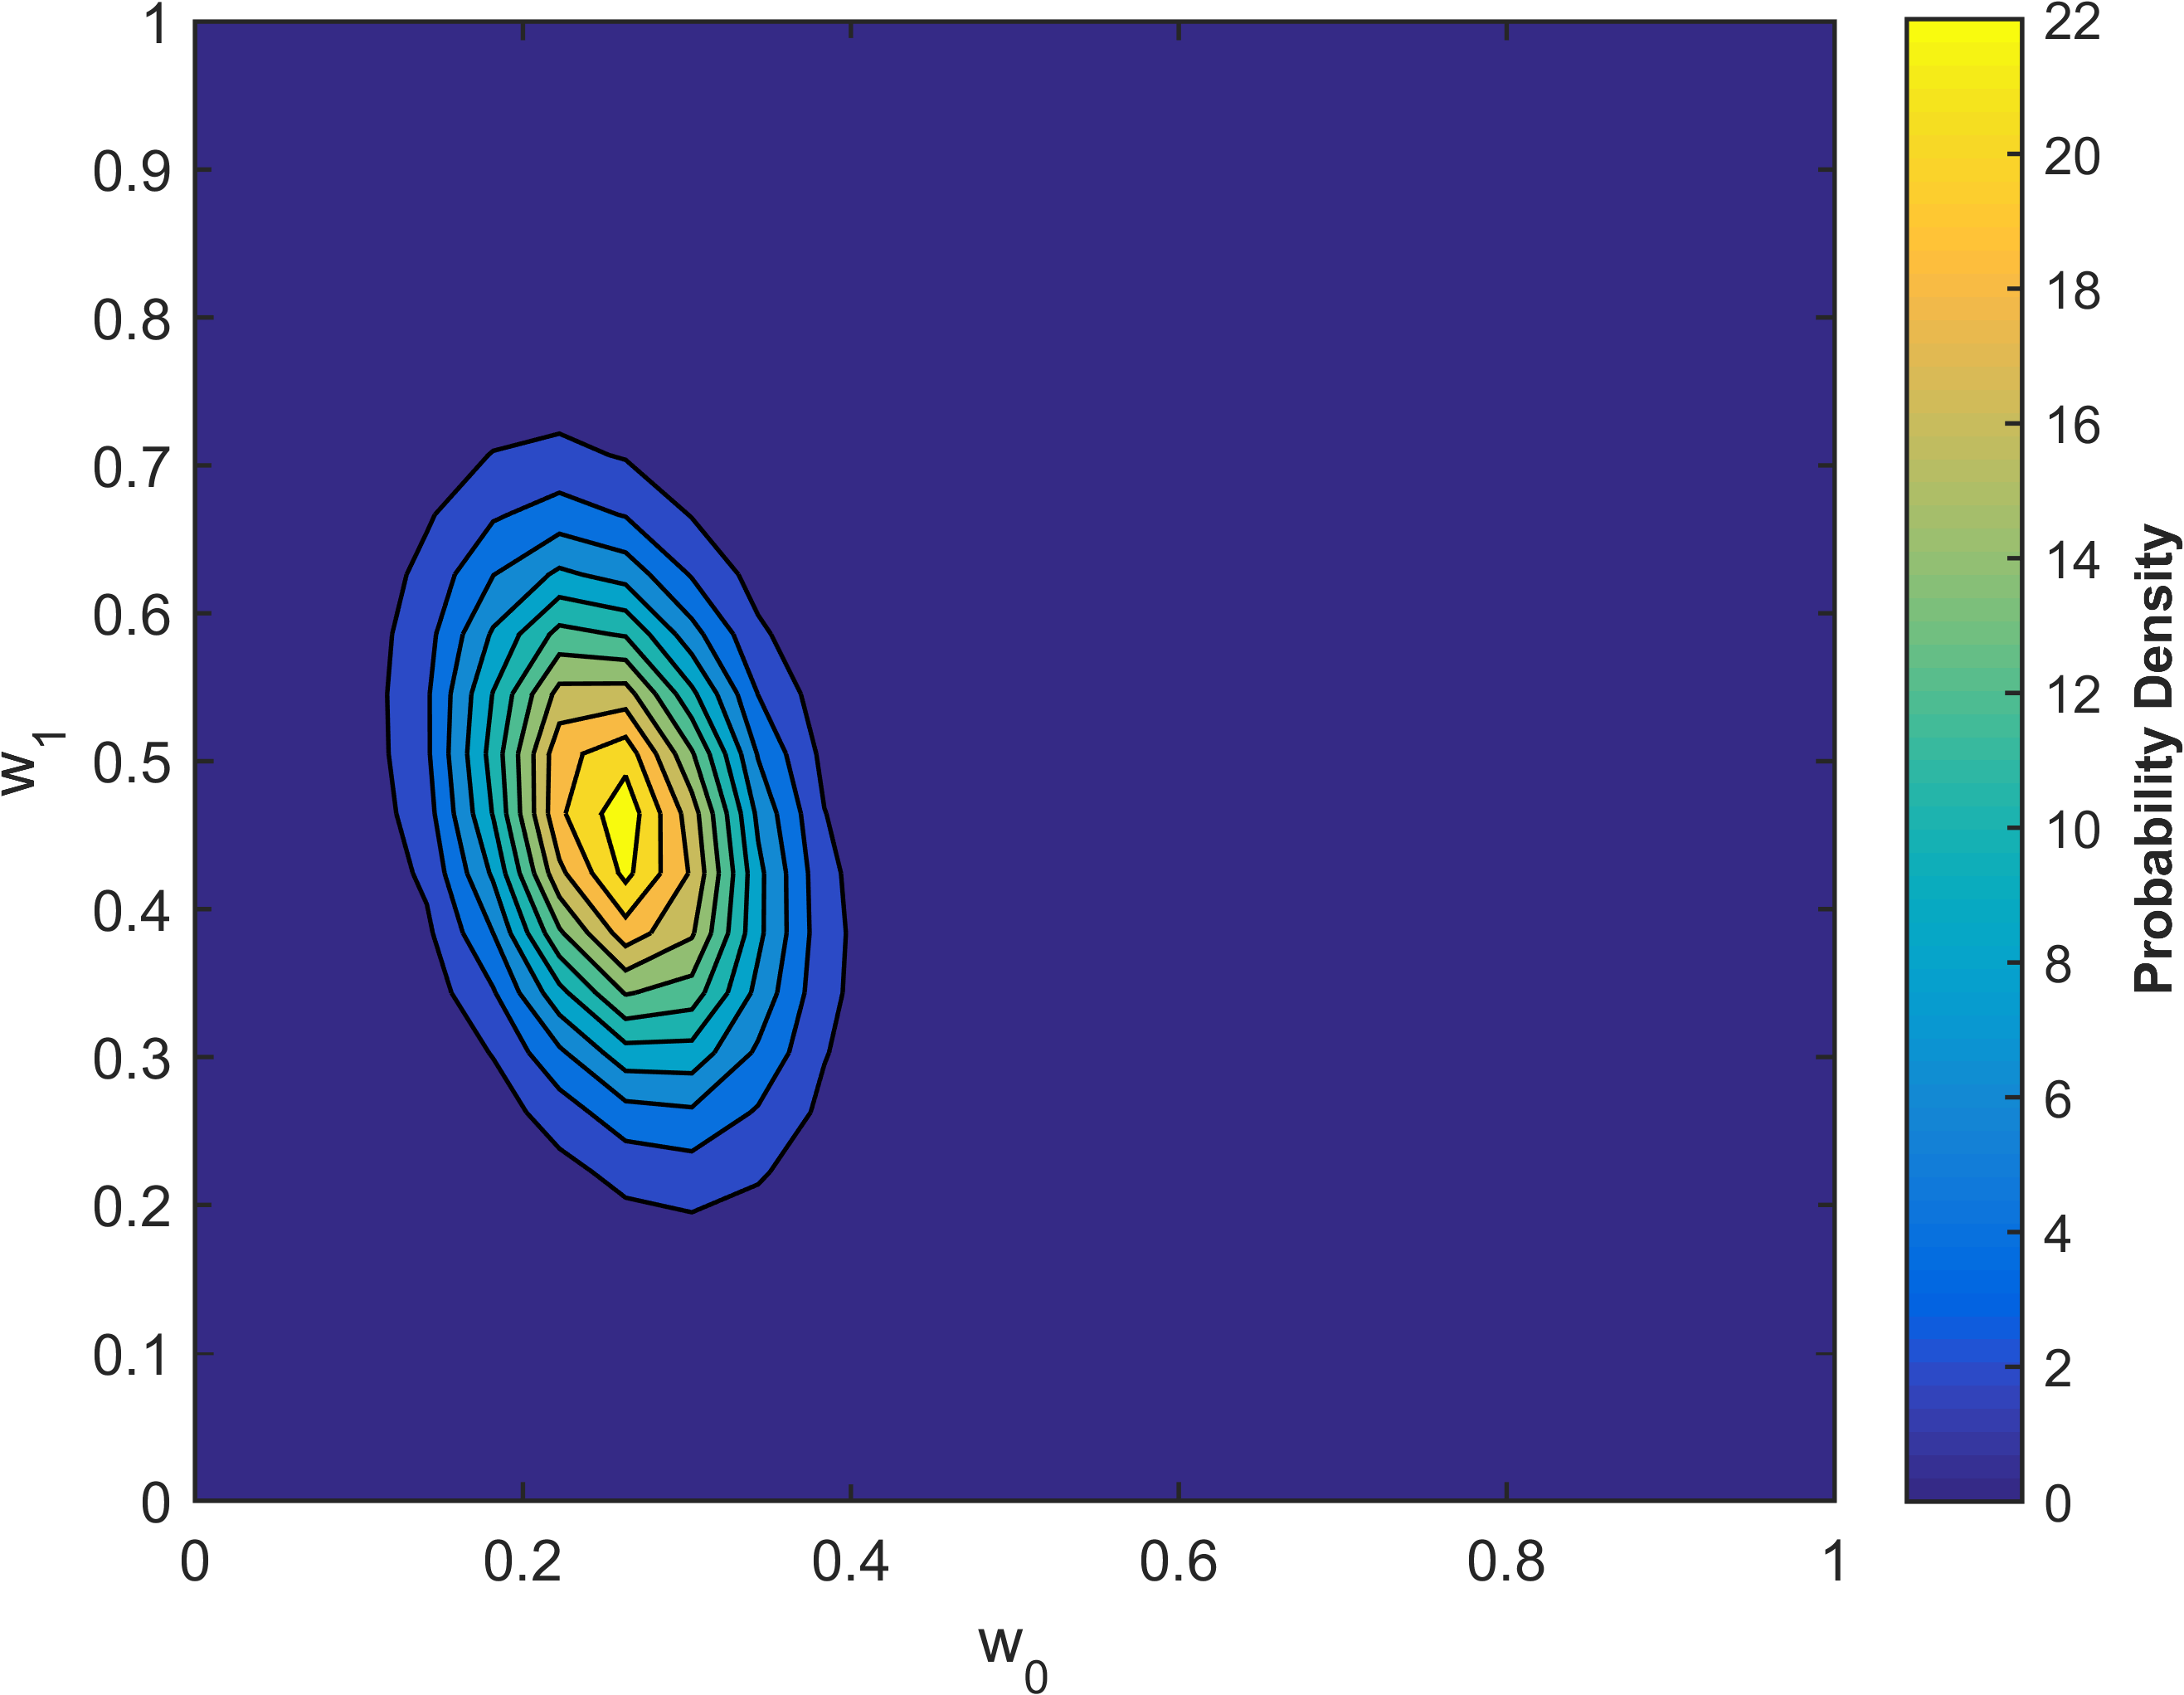
\includegraphics[width=0.29\textwidth]
        {images/part1/posteriorBLR}
        \label{subFigposteriorBLR}
  }\quad
\subfigure[{Linear Prediction based on the posterior, given the Dataset $\mathcal{D}_{1}$ prior $\Sigma_{P}$and noise $\sigma_{n}$. The predicted linear line does not pass through the data points but between them.}]
  {
        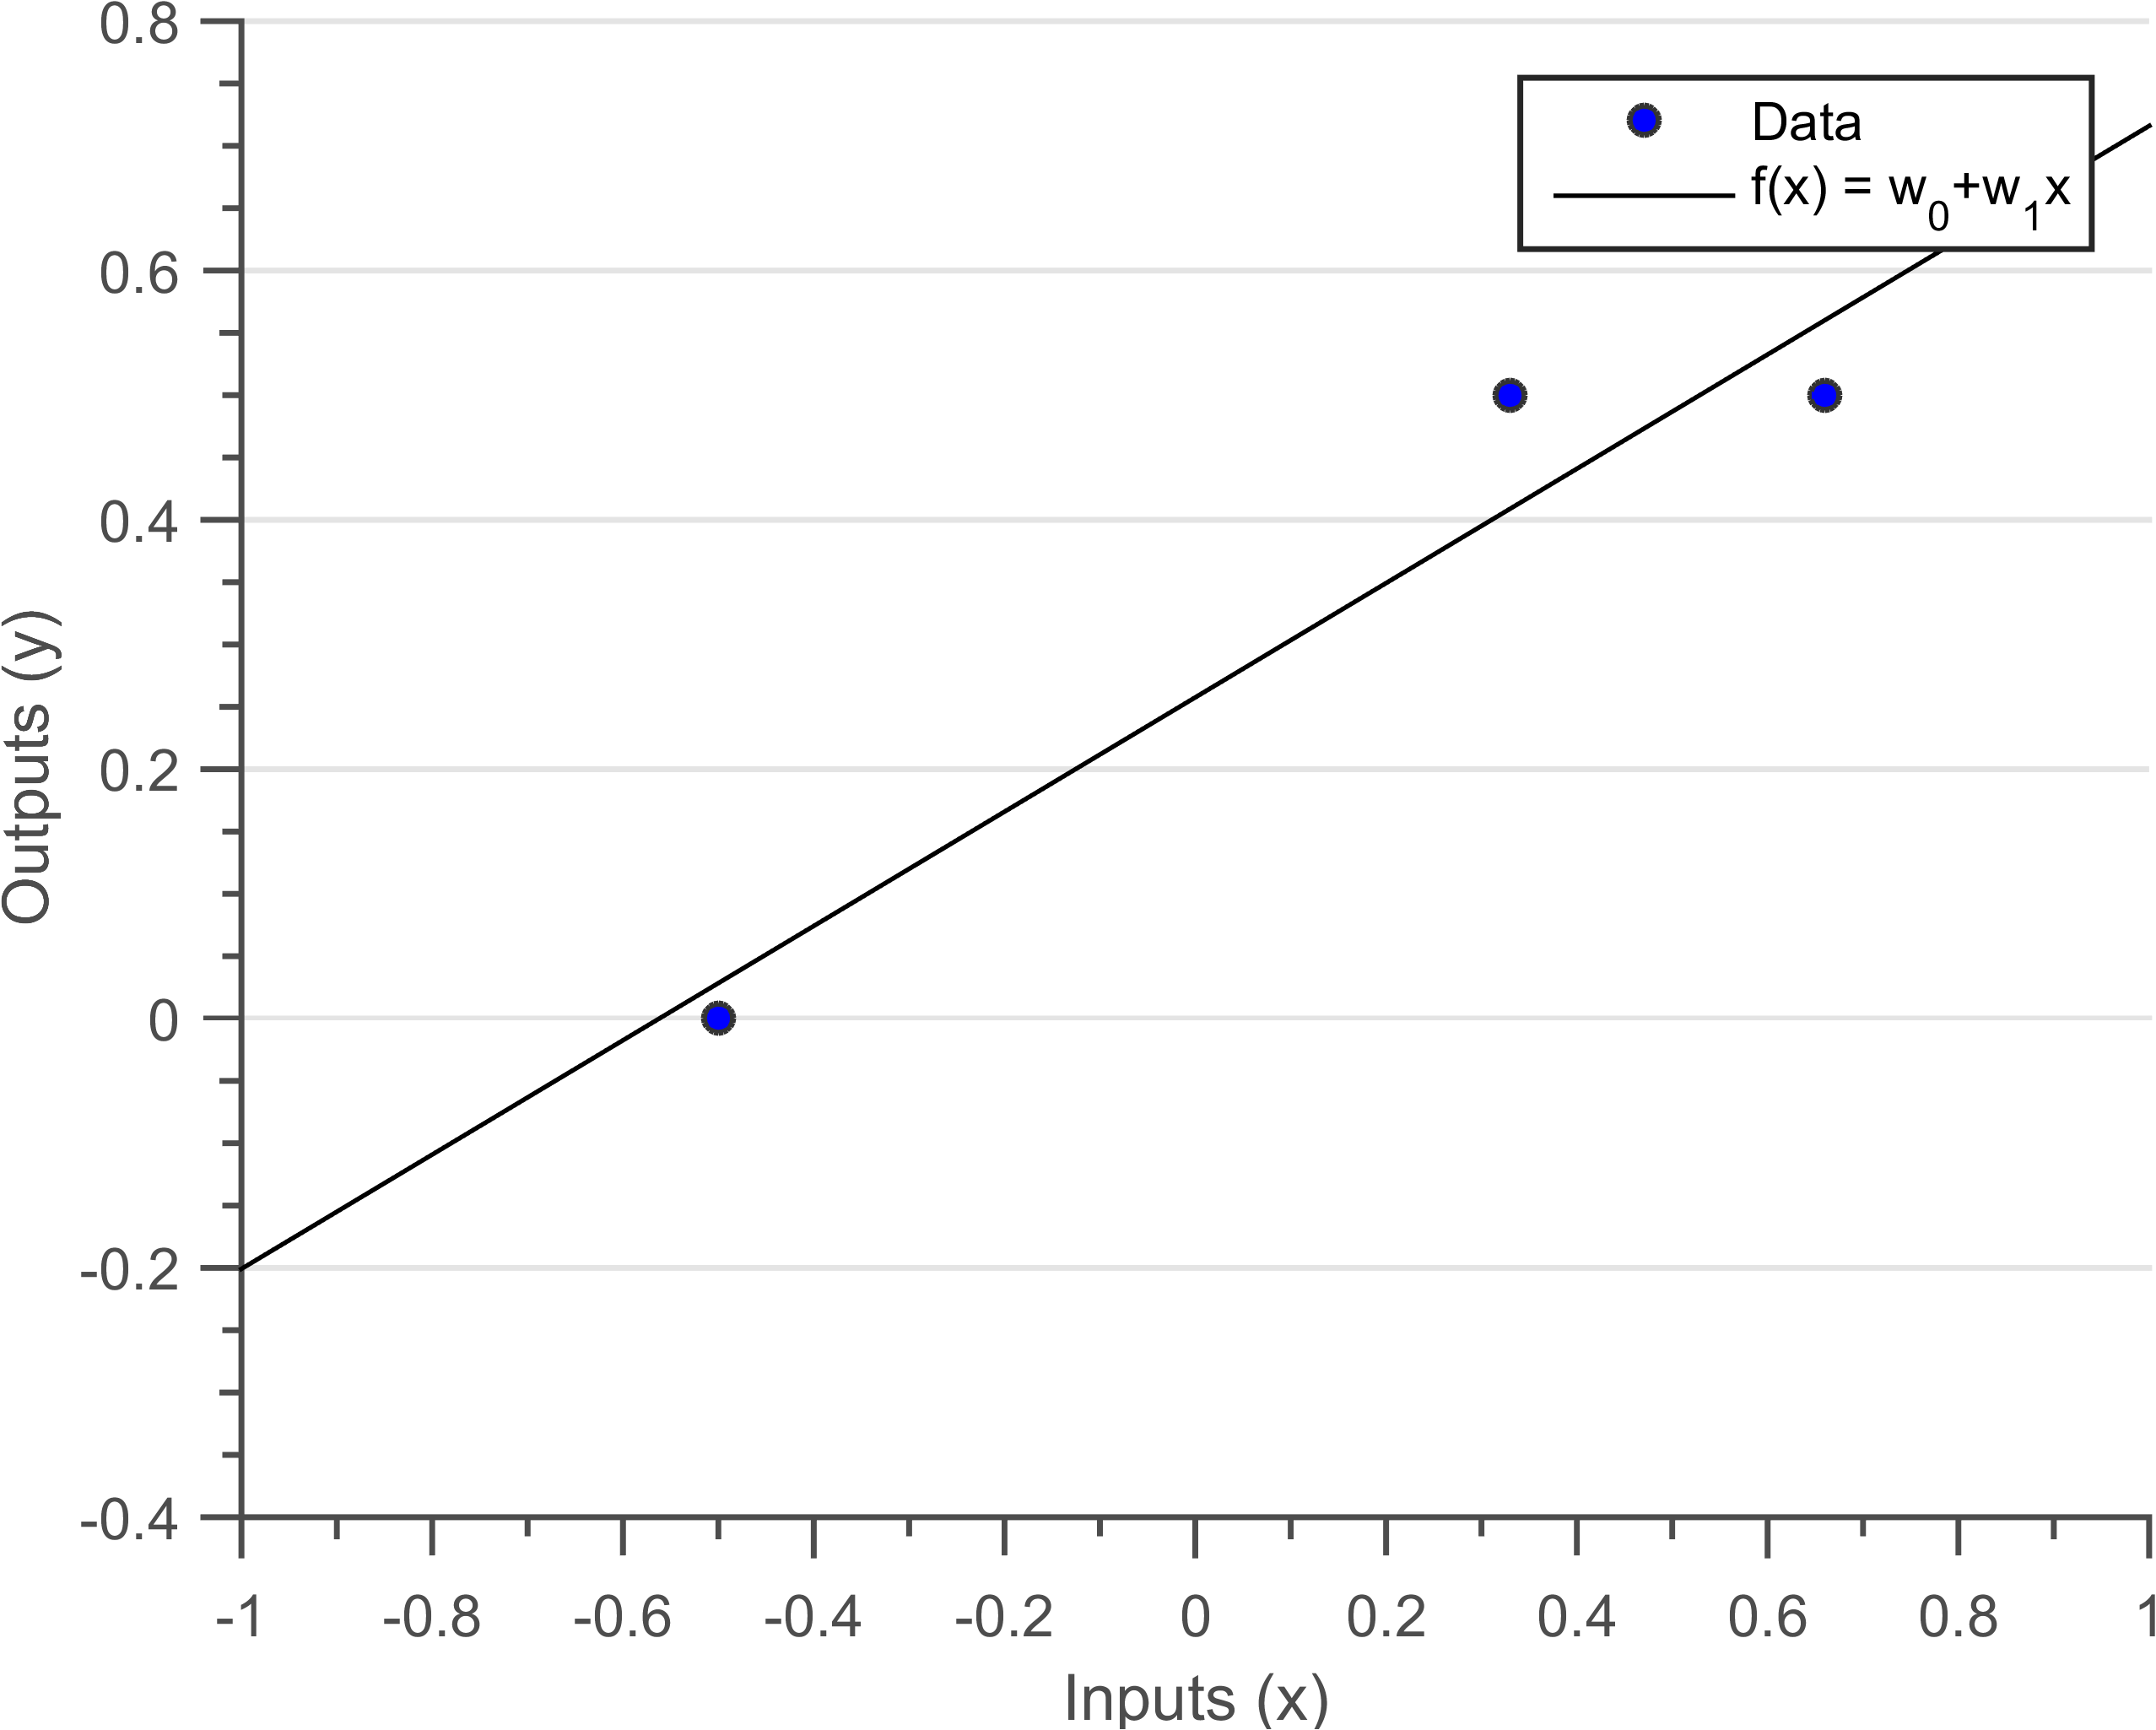
\includegraphics[width=0.29\textwidth]
        {images/part1/predictionsBLR}
        \label{subFigpredictionsBLR}
  }\quad
       \caption{Prior, Posterior and Prediction in Bayesian Linear Regression}
       \label{figPriorAndPosterior}
\end{figure}

While the Bayesian Linear Regression framework provides an opportunity to encode prior assumptions in terms of distributions of the parameters. A much more elegant and expressive method is by using Gaussian Processes to perform regression. Gaussian Processes are a distribution over functions and hence enable us to encode prior knowledge directly in the functional space. 

\marginnote{\textsl{Non-parametric models}}[1cm]
Learning algorithms are mainly divided into two main types. The first is defined by parametric models which can only represent a limited hypothesis space. They use parameters to describe the function between input and output domain. For example the weight parameters $w$ in Bayesian Linear Regression. The second are non-parametric models whose hypothesis space grows with the size of data \cite{ghahramani2013bayesian}. Non-parametric models use data to represent functions, Gaussian Process Regression is a type of non-parametric model. One can imagine a non-parametric model like a stretched rubber sheet: whenever it sees data it deforms accordingly to compensate for the new data point. Hence the more data it sees the more it starts mimicking the actual function. 

\marginnote{\textsl{Gaussian Process}}[1cm]
Gaussian Process or Kriging was first used in the context of Geo-statistics research by Daniel Krige \cite{krige1951statistical}, this was later formalized by Matheron in his seminal work "Principals of Geo-statistics" \cite{matheron1963principles}. Recently, interest in the Gaussian Process (GP) grew in the machine learning community from neural networks research. It was shown that a Bayesian neural network becomes a Gaussian process as the number of neurons tends to infinity \cite{neal2012bayesian}. Gaussian processes are probabilistic distributions over functions, which provide a Bayesian non-parametric approach to smoothing and interpolation. A Gaussian Process can be fully parameterized by its mean and covariance function. More generally, a Gaussian Process is a method to probabilistically define a family of functions, chapter \ref{chapGp} expands GP in more detail. 

\section{Outline}\label{secOutline}
This thesis is divided into three main parts, each part is then divided into individual chapters and their constituent sections. This part sets up the prerequisites required to understand the concepts introduced in the next two parts. The first chapter demonstrates the need for performing regression in aircraft design tasks and describes a very basic Bayesian Linear Regression scheme. 

\marginnote{\textsl{Chapter \ref{chapGp}}}[1cm]
Chapter \ref{chapGp} shows the key processes involved in a GP regression framework. GPs as distributions over functions have a rich history in geo-statistics and machine learning. The second chapter heavily draws ideas from \cite{krige1951statistical, matheron1963principles} of the geo-statistics community and \cite{Stein1999Springer, kennedy2000predicting, Rasmussen2005, mackay2003information} of the machine-learning community, showing a process flow of how to perform regression using GPs. The remaining chapter unfolds as follows, section \ref{secPrior} describes the key constituents of a GP and how to draw random functions from a GP. Section \ref{secPosterior} describes how to perform prediction in presence and absence of measurement noise. Section \ref{secHyperParameter} introduces marginal likelihood as a form of evaluation method to automatically choose hyper-parameters. 

\marginnote{\textsl{Chapter \ref{chapScalingGPR}}}[1cm]
Chapter \ref{chapScalingGPR} deals with the problem of scaling GP regression to massively many points. Traditional GPs are computationally infeasible on a standard laptop if the number of data points increase $\mathcal{O}(10^4)$. There exist two main methods to scale a GP regression, one using reduced set of inducing points while another based on mixture of experts methodology. This chapter draws heavily from the works of \cite{quinonero2005unifying, seeger2003fast, Snelson06sparsegaussian, Titsias09variationallearning} for the approximation method of inducing points and \cite{cao2014generalized, tresp2000bayesian, chen2009bagging, deisenroth2015distributed} for the approximation method of mixture of experts, please refer to the individual publications for more detail. We demonstrate the limitations and capabilities of both the methods on a toy dataset, giving directions to choosing optimal parameters and extracting the best possible result.  

\textbf{Description of the other two parts}

%%% Local Variables: 
%%% mode: latex
%%% TeX-master: "isae-report-template"
%%% End: 

\chapter{Gaussian Process Regression}
\label{chapGp}

Suppose we perform a simulation or experiment on an input point $x_{j} \in \mathbb{R}^{D_{inputs}}$and measure an output $y_{j} \in \mathbb{R}$. In this chapter we assume that the input is $D_{inputs}$ dimensional and the output is one dimensional. We can thus have a data set of $N$ observations, $\{\mathcal{D} = (x_{j}, y_{j}) | j \in [1; N] \}$. The full input and output vectors can be denoted as $X = \{x_{1}; x_{2}; \ldots ; x_{N}\}$ and $Y = \{y_{1}; y_{2}; \ldots ; y_{N}\}$ such that $X \in \mathbb{R}^{N \times P}$ and $Y \in \mathbb{R}^{N }$. Given this data we are interested in making predictions for new input points $x_{*}$ \footnote{Also called as test point, prediction point or target point.}that are not present in our series of experiments. This means that we need to use out training data and learn, the true physical process  $f(x)$ that generates our data set.

As discussed in the previous chapter, to learn the governing function $f(x)$ we first start with a family of functions. Gaussian Process (GP) can be used to probabilistically define a family of functions. More formally, a GP is a distribution over functions such that any finite set of function values $[f(x_{1}), f(x_{2}), \ldots, f(x_{N})]$ have a joint Gaussian distribution \cite{rasmussen2006gaussian}. 

\marginnote{\textsl{Infinite dimensional random vector}}[1cm]
While a normal distribution describes a scalar random variable, example $X \sim \mathcal{N}(0, 1)$ defines a Gaussian variable with mean $0$ and variance $1$. A multi variate distribution defines a vector of random variables, for example $\{X\} \sim \mathcal{N}(\{0, 0\}, [1, 0; 0, 1])$ defines a Gaussian vector with mean $\{0, 0\}$ and covariance $[1, 0; 0, 1]$. A GP is the extension of this concept in the functional space. We can also think of a function as an infinite dimensional vector, each entry in the vector specifying the function value $f(x)$ at a particular point $x$ \footnote{Yes blew my mind as well!}. 

\marginnote{\textsl{Mean}}[1cm]
A GP model before conditioning on data can be completely parameterized by its mean

\begin{equation}\label{eq:meanGP}
\mathbf{E}[f(x)] = m(x)
\end{equation}

\marginnote{\textsl{Covariance}}[1cm]
and its covariance function also called a kernel. In the context of the GPs a kernel is a measure of similarity between pairs of functional values $(f(x))$ evaluated at input points , often involving an inner product of basis functions $\phi(x)$ \cite{bishop2006pattern}. Please refer to chapter \ref{chapBasicCovarianceKernels} for a more detailed insight into kernels.   \footnote{The terms covariance functions, kernel and kernel functions will be used interchangeably during the reminder of this thesis}:

\begin{equation}\label{eq:covarianceGP}
Cov[f(x) - m(x), f(x') - m(x')] = k(x_{1}, x_{2})
\end{equation}

We can formally write the probability of the function $f$ as:

\begin{equation}\label{equationGPdefinition}
\Pr[f(x)] = GP(m(x), k(x_{1}, x_{2}))
\end{equation}

The notation $\Pr(f( x))$ symbolizes probability distribution of function $f$ at the inputs $x$. A function randomly drawn from a GP yields a random function around the mean function $m(x)$ and of the shape as defined by covariance function $k(x_{1}, x_{2})$. 

\marginnote{\textsl{Tractable}}[1cm]
Performing inference on an infinite dimensional vector (function) can be a computationally intensive task. Thankfully, due to the marginalization property of Gaussians, if we ask for properties of the function at a finite number of points, then  GP will give us the same answer if we ignore the infinitely many other points. In other words any finite set of function values $[f(x_{1}), f(x_{2}), \ldots, f(x_{N})]$ have a joint Gaussian distribution in GP (also the  definition of GP). This property means that GP specified in equation \ref{equationGPdefinition} also specifies equation \ref{equationGPMarginalizationProperty}. This makes GPes computationally tractable, one of the major benefits of GP. 


\begin{equation}\label{equationGPMarginalizationProperty}
\Pr\left [ \begin{matrix}
f(x_{1})
\\ f(x_{2})
\end{matrix} \right ] = \mathcal{N}\left (\left [ \begin{matrix}
m(x_{1})
\\ m(x_{2})

\end{matrix} \right ] , \left [ \begin{matrix}
k(x_{1}, x_{1}) & k(x_{1}, x_{2})\\ 
k(x_{2}, x_{1}) & k(x_{2}, x_{2})
\end{matrix} \right ] \right )
\end{equation}

While performing regression in a GP framework we first define a family of functions also called prior (section \ref{secPrior}). The next step involves taking observations and eliminating all the functions in our prior which do not obey the observations, this step gives us the posterior mean and variance (section \ref{secPosterior}). Finally, we can further improve our predictions by fine-tuning our hyper-parameters (section \ref{secHyperParameter}).

\section{Prior} \label{secPrior}
In the Bayesian framework, a prior is a probability distribution before looking at any evidence. In the context of a GP Regression, this is provided by the mean and covariance function. 

\subsection{Hyperparameters}
Both mean and covariance functions are specified by a set of hyper-parameters $\theta$. The hyper-parameters are very similar to weight parameter ($w$) during Bayesian Linear Regression (section \ref{secBayesianModelling}), these are the parameters of the GP. Selecting a prior in GP boils down to choosing an appropriate functional form of the mean and covariance matrix and then choosing the hyper-parameters of the prior \cite{duvenaud2013structure}. 

Automatically, predicting the values of hyper-parameters is important to choose a good prior. We will look at how to choose good hyper-parameters in section \ref{secHyperParameter}. 

\subsection{Mean function}\label{subSecCH2MeanFunction}
The mean function $m(x)$ of a GP represents its trend. In Universal Kriging, we usually choose a mean function of the form $m(x) = \phi(x)^{T}\theta$, with $\phi(x) = (\phi_{1}(x), \ldots , f_{p}(x))$ being a vector of basis functions, generally including a constant function and $\theta \in \mathbb{R}^{p}$ is a vector of hyper-parameters \cite{matheron1963principles}. In Simple Kriging we assume a constant mean function $m(x) = \theta$.

\marginnote{\textsl{Zero mean}}[1cm]
Without loss of generality, we can assume the mean function to be zero everywhere, since uncertainty about the mean function can be taken into account by adding an extra term to the covariance function (Chapter \ref{chapBasicCovarianceKernels}).  

\begin{equation}\label{equationMeanZeroGPdefinition}
\Pr[f(x)] = GP(0 , k(x_{1}, x_{2}, \theta))
\end{equation}

We assume a zero mean prior through out this section. After accounting for the zero mean, the GP model can be completely parametrized by the kernel. Hence the problem of learning in a GP is exactly the problem of finding suitable properties of the covariance function \cite{rasmussen2006gaussian} (equation \ref{equationMeanZeroGPdefinition}). 

\textbf{Comment about the code}
\begin{mdframed}[hidealllines=true,backgroundcolor=lightgray!20]
\begin{lstlisting}[caption={A zero mean function}, 
                    captionpos=b, 
                    label={codeMeanFunction},
                    style=Matlab-editor, 
                    backgroundcolor = \color{MatlabCellColour}]
% zero mean function
meanFunction = @(x) 0*x; 

\end{lstlisting}
\end{mdframed}

\subsection{Covariance function}\label{subSecCH2Covariance}
The covariance function is a positive definite kernel, such that for any $a_{i} \in \mathbb{R}$ equation \ref{equationPDKernel} holds \cite{Stein1999Springer}.

\begin{equation}\label{equationPDKernel}
\sum_{i=1}^{N}\sum_{j=1}^{N}a_{i}a_{j}k(x,x') \geq 0
\end{equation}

A popular choice of covariance function is a Squared Exponential (SE) function (equation \ref{eqnSquaredExponential}), because it defines a family of highly smooth (infinitely differentiable) non-linear functions as shown in figure \ref{figGPPriors}.

\begin{equation}\label{eqnSquaredExponential}
k_{SE}(x_{1}, x_{2}, \theta) = \theta_{amplitude}^2exp[-\frac{d^2}{2\theta_{lengthScale}^2}]
\end{equation}

\marginnote{\textsl{SE kernel}}[1cm]
For the case of the SE kernel the hyper-parameters $(\theta = [\theta_{amplitude}, \theta_{lengthScale}])$ are; amplitude $(\theta_{amplitude})$ which defines average distance from mean and the length scale $(\theta_{lengthScale})$ which defines the smoothness of functions. Here, $d$ defines the absolute distance between points $|x-x'|$. Covariance functions which are purely a function of distance $d$ are called as isotropic stationary functions. These covariance functions remains unchanged if the points $x_{1}, x_{2}$ are rotated or translated. Hence a family of functions defined by stationary kernels will have similar local features throughout the input domain. 

\marginnote{\textsl{Length-Scale}}[1cm]
When $x$ tends to $x'$ then $k(x_{1}, x_{2})$ approaches $\theta_{amplitude}^{2}$, this means that $f(x)$ is highly correlated with $f(x')$. This is a good characteristic for smooth functions, since points in the neighbourhood must be alike. If $x$ is far away from  $x'$ then $k(x_{1}, x_{2})$ tends to zero, this means that far away points are loosely correlated. Hence, far off observations will have negligible effect while performing interpolations. How fast or slow the covariance decreases with distance depends on the length scale parameter $\theta_{lengthScale}$, smaller length-scale means a faster moving function. In general we cannot extrapolate more than $\theta_{lengthScale}$ units from the closest data-point \cite{duvenaud-thesis-2014}. 

\textbf{comment about the code}
\begin{mdframed}[hidealllines=true,backgroundcolor=lightgray!20]
\begin{lstlisting}[caption={A Standard Exponential covariance function}, 
                    captionpos=b, 
                    label={codeCovarianceFUnction},
                    style=Matlab-editor, 
                    backgroundcolor = \color{MatlabCellColour}]
% Standard exponential covariance function
covarianceFunction = @(theta, x1, x2)(theta(1).^2*exp(-(x1 - x2)^2/(2*theta(2).^2))); 
% theta(1): is the amplitude hyperparameter
% theta(2): is the length-scale hyperparameter
\end{lstlisting}
\end{mdframed}

\subsection{Sampling functions from GP priors}\label{subSecSamplingFunctionsGPPrior}
To have a look at the constituent functions in a prior we can randomly sample functions from the GP. Since any finite set of set of function values have a joint Gaussian distribution in a GP. To draw random functions from a GP we choose $N*$ input points $X_{*} = \{x_{1*}; x_{2*}; \ldots ; x_{N*}\}$ and write corresponding mean vector $m(X_{*})$ and covariance matrix $K(X_{*}, X_{*} )$ \footnote{The covariance matrix is also called the Gram matrix} using equation \ref{equationGPMarginalizationProperty} and \ref{eqnSquaredExponential}. We then generate a random Gaussian vector $f(X_{*})$ for this multi-variate Gaussian (equation \ref{equationMeanZeroGPdefinition}) and plot the generated values as a function of inputs $X_{*}$. 

\begin{equation}\label{eqnCovMatrixSquaredExponential}
K(X_{*}, X_{*} ) = \left [ \begin{matrix}
k(x_{1*}, x_{1*}) & k(x_{1*}, x_{2*}) & \ldots & k(x_{1*}, x_{N*})
\\ k(x_{2*}, x_{1*}) & k(x_{2*}, x_{2*}) & \ldots & k(x_{2*}, x_{N*})
\\ \vdots & \vdots & \ddots & \vdots
\\ k(x_{N*}, x_{1*}) & k(x_{N*}, x_{2*}) & \ldots & k(x_{N*}, x_{N*})
\end{matrix} \right ] 
\end{equation}

\textbf{comment about the code}

\begin{mdframed}[hidealllines=true,backgroundcolor=lightgray!20]
\lstinputlisting[caption={Plotting the Gram Matrix}, 
                    captionpos=b, 
                    label={codeGramMatrix}, 
                    backgroundcolor = \color{MatlabCellColour}, 
                    style=Matlab-editor]
                    {codes/chapter2/gramMatrix.m}
\end{mdframed}

Figure \ref{figGPCovarianceMatrix} shows the covariance matrix for Standard Exponential kernel with different hyper-parameters at the input points $X^{*} = \{[0:0.02:1]\}$. The SE kernel of figure \ref{subFigcovSEmatrix_1} has a lower length-scale than figure \ref{subFigcovSEmatrix_2}. Note, how the covariance values are more spread out for figure \ref{subFigcovSEmatrix_2}.

\begin{figure}[!ht]
  \centering
    \subfigure[{Covariance matrix for a Standard Exponential (SE) Kernel with $(\theta = [1, 0.2])$ at the input points $X^{*} = \{[0:0.02:1]\}$. }]
  {
        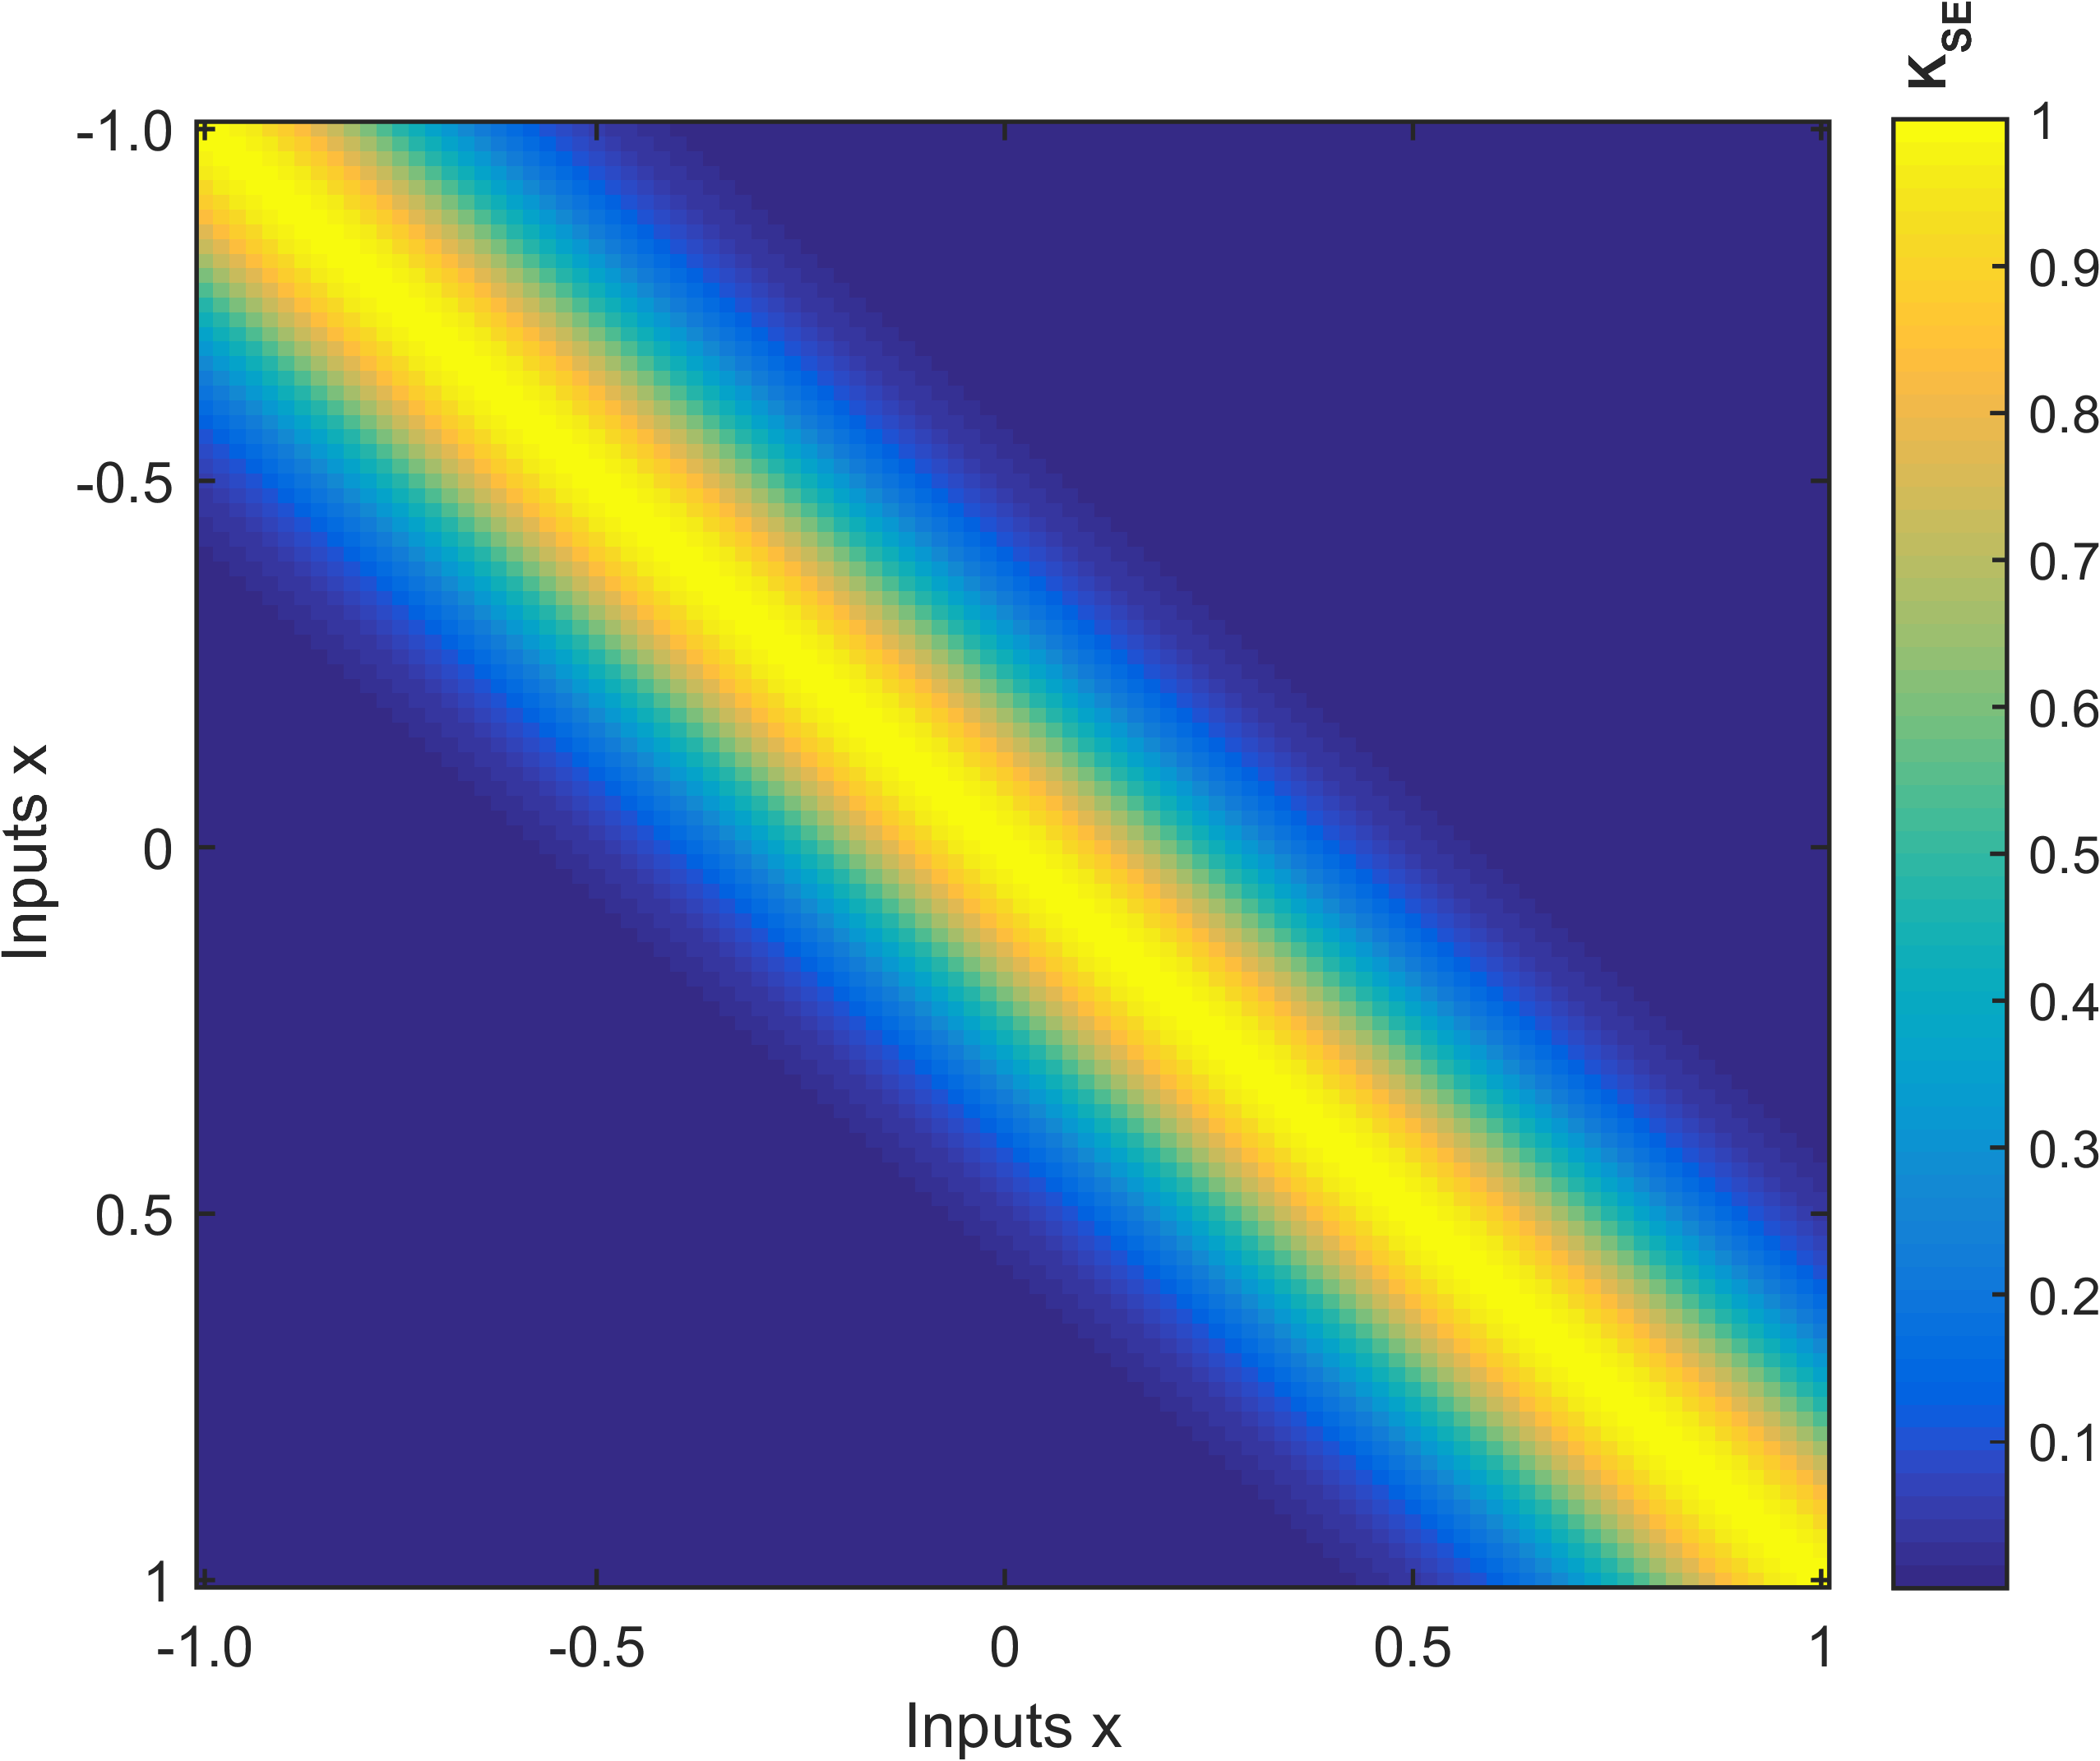
\includegraphics[width=0.45\textwidth]
        {images/part1/covSEmatrix_1}
        \label{subFigcovSEmatrix_1}
  }\quad
\subfigure[{Covariance matrix for a Standard Exponential (SE) with $(\theta = [1, 0.5])$ at the input points $X^{*} = \{[0:0.02:1]\}$}]
  {
        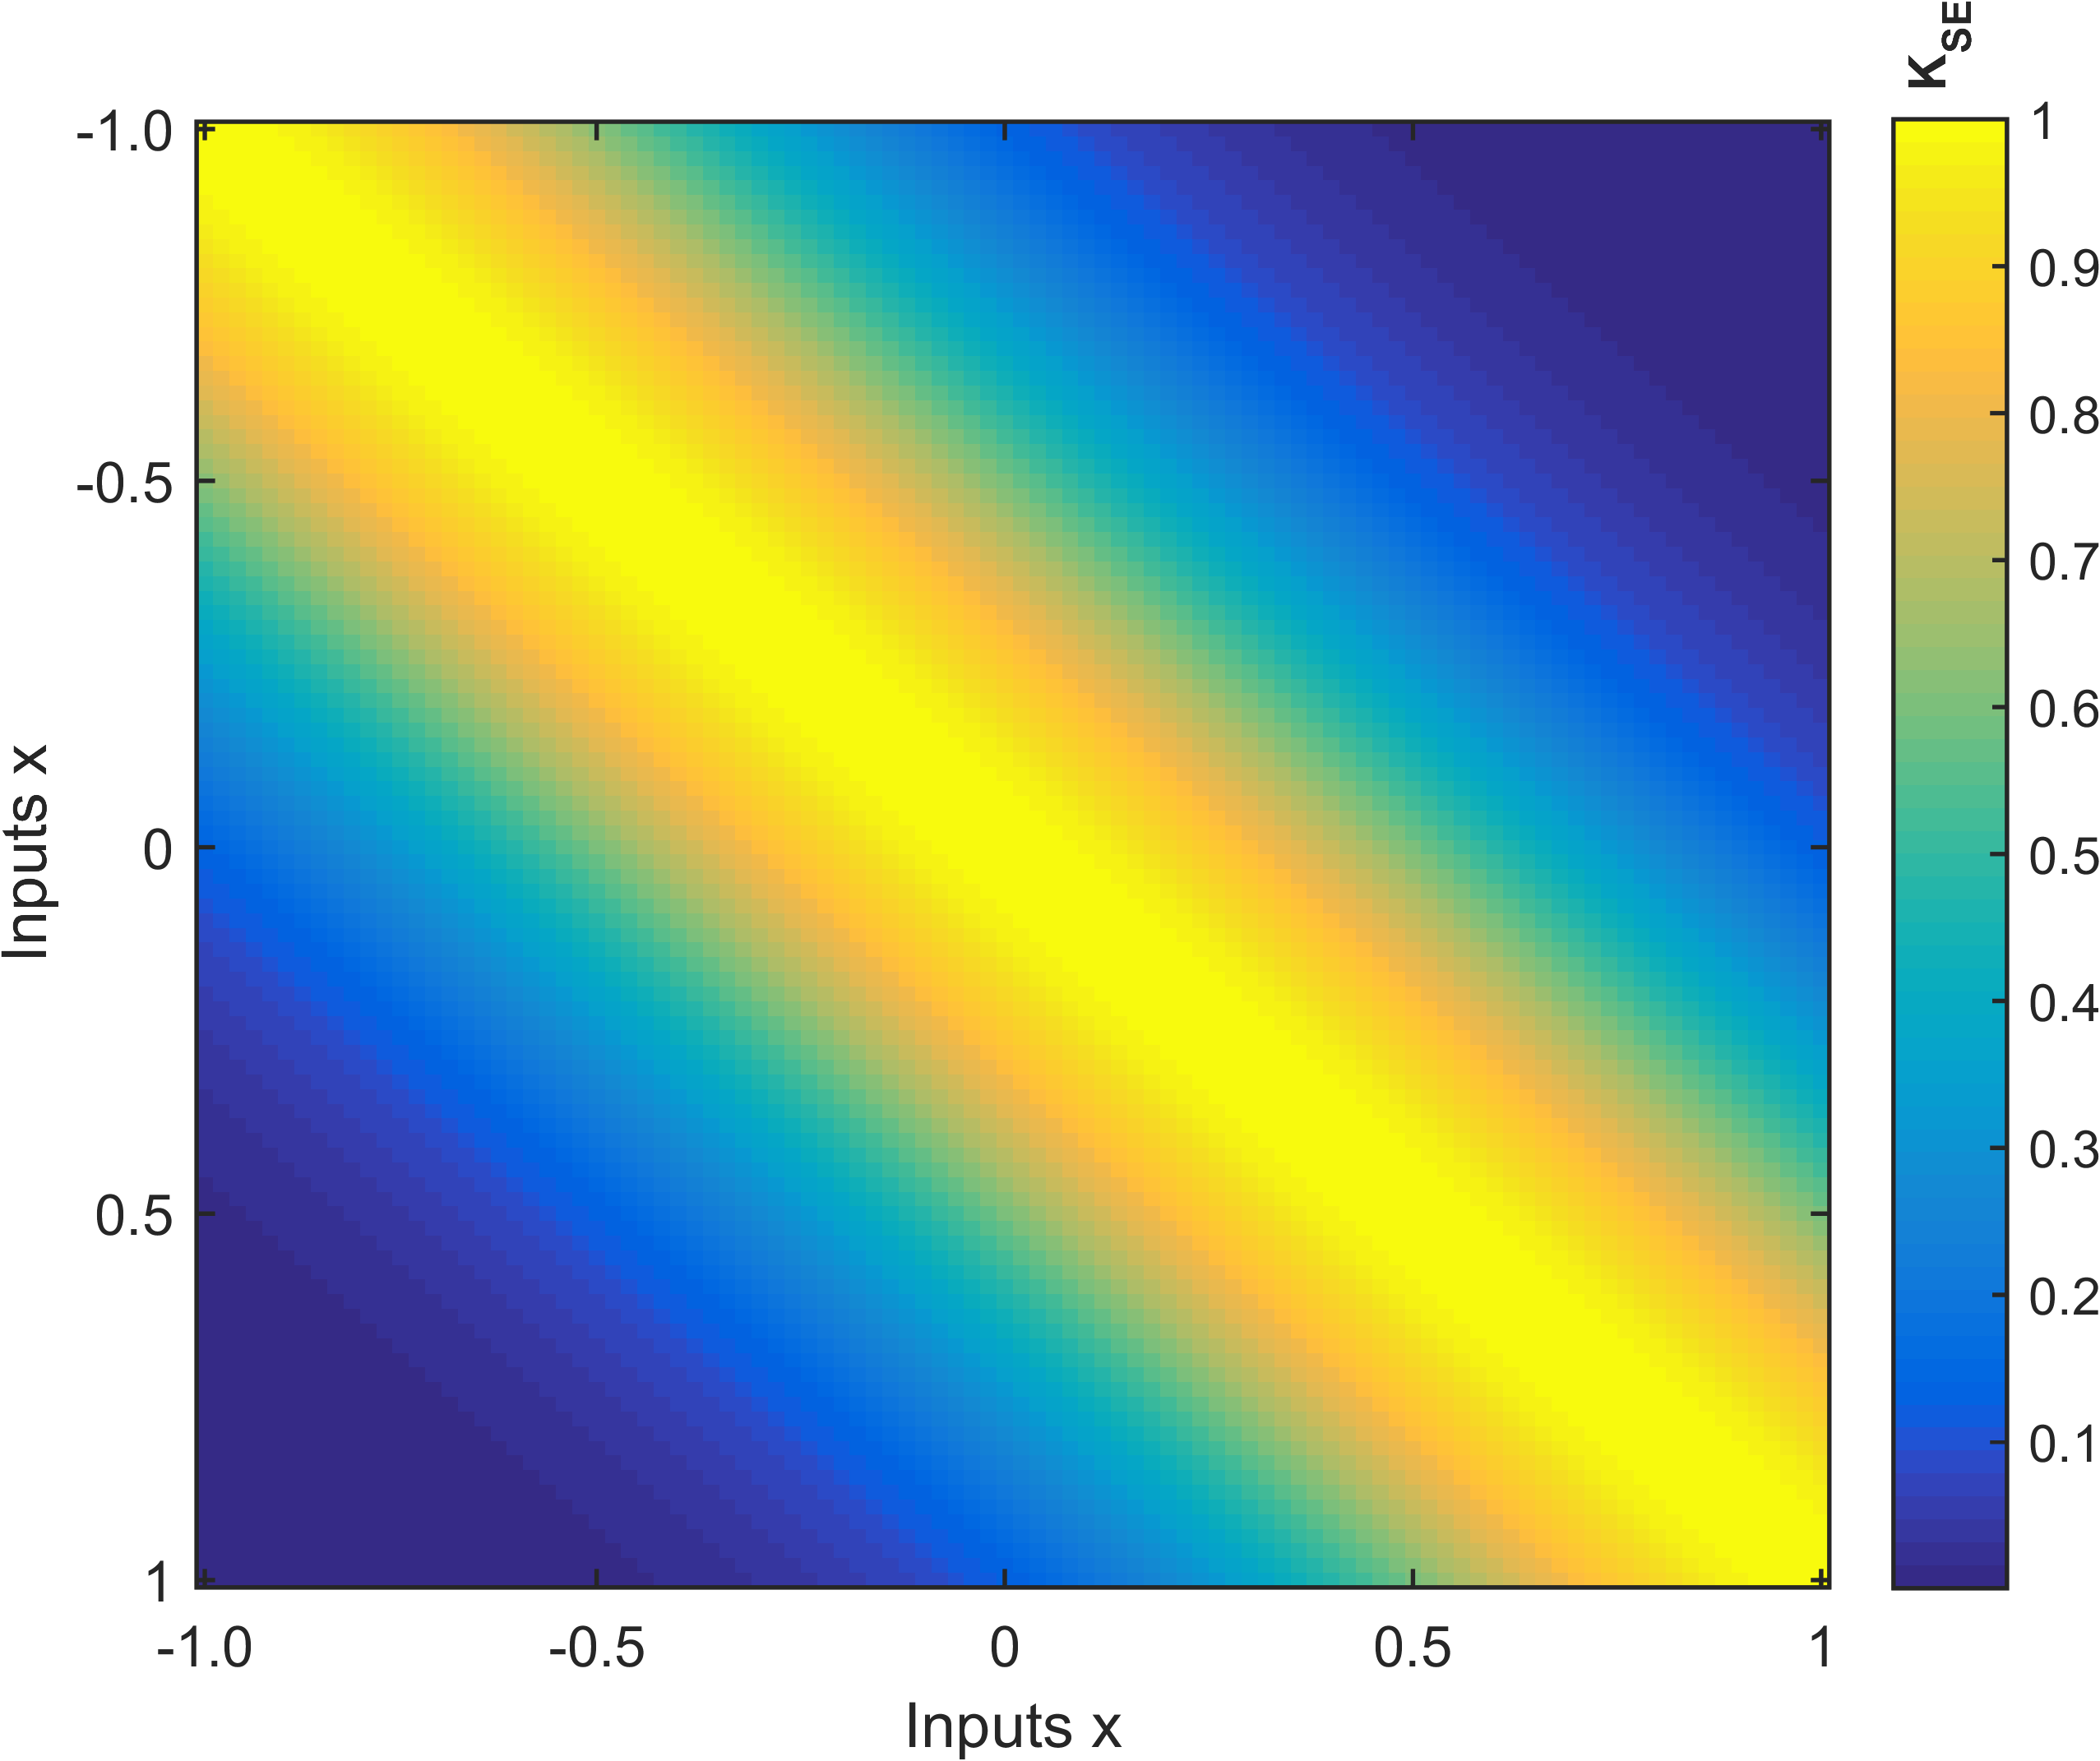
\includegraphics[width=0.45\textwidth]
        {images/part1/covSEmatrix_2}
        \label{subFigcovSEmatrix_2}
  }\quad
  
       \caption{Covariance matrix for a Standard Exponential kernel with different hyper-parameters at the input points $X^{*} = \{[0:0.02:1]\}$. The SE kernel of figure \ref{subFigcovSEmatrix_1} has a lower length-scale than figure \ref{subFigcovSEmatrix_2}. Note, how the covariance values are more spread out for figure \ref{subFigcovSEmatrix_2}.}\label{figGPCovarianceMatrix}
\end{figure}

To generate a random Gaussian vector $f(X_{*})$ of length $N_{*}$, we first calculate the Cholesky decomposition\footnote{Cholesky Decomposition is also called the square-root of matrix and is defined for positive definite matrices} of the covariance matrix $K(X_{*}, X_{*}) = LL^{T}$, where $L$ is a lower triangular matrix. We then generate a random vector $U$, such that $U = \mathcal{N}(0, I)$ and $I$ is an identity matrix of size $N_{*}$.  The random vector can be then computed as, $f(X_{*}) = m(X_{*}) + LU$ and when plotted with the inputs $X_{*}$ gives a randomly drawn function. 

\textbf{Comment about the algorithm}
% Adding the algorithm
\begin{mdframed}[hidealllines=true,backgroundcolor=lightgray!20]
\lstinputlisting[caption={Sampling a random function from the prior}, 
                    captionpos=b, 
                    label={codeSamplingFUnction}, 
                    backgroundcolor = \color{MatlabCellColour}, 
                    style=Matlab-editor]
                    {codes/chapter2/samplingFunctionFromAPrior.m}
\end{mdframed}

Figure \ref{figGPPriors} shows 5 random functions drawn for a zero mean GP with the covariance matrices of figure \ref{figGPCovarianceMatrix}. The solid black line defines the mean function, shaded blue region defines 95\% confidence interval (2$\sigma$) distance away from the mean. The dashed lines are five functions drawn at random from a GP prior. We can observe that figure \ref{subFigSEPrior_1} varies faster when compared to figure \ref{subFigSEPrior_2} due to smaller length scale hyper-parameter. 

\begin{figure}[!ht]
  \centering
    \subfigure[{Draws from a GP prior with mean zero and Standard Exponential (SE) Kernel with $(\theta = [1, 0.2])$. }]
  {
        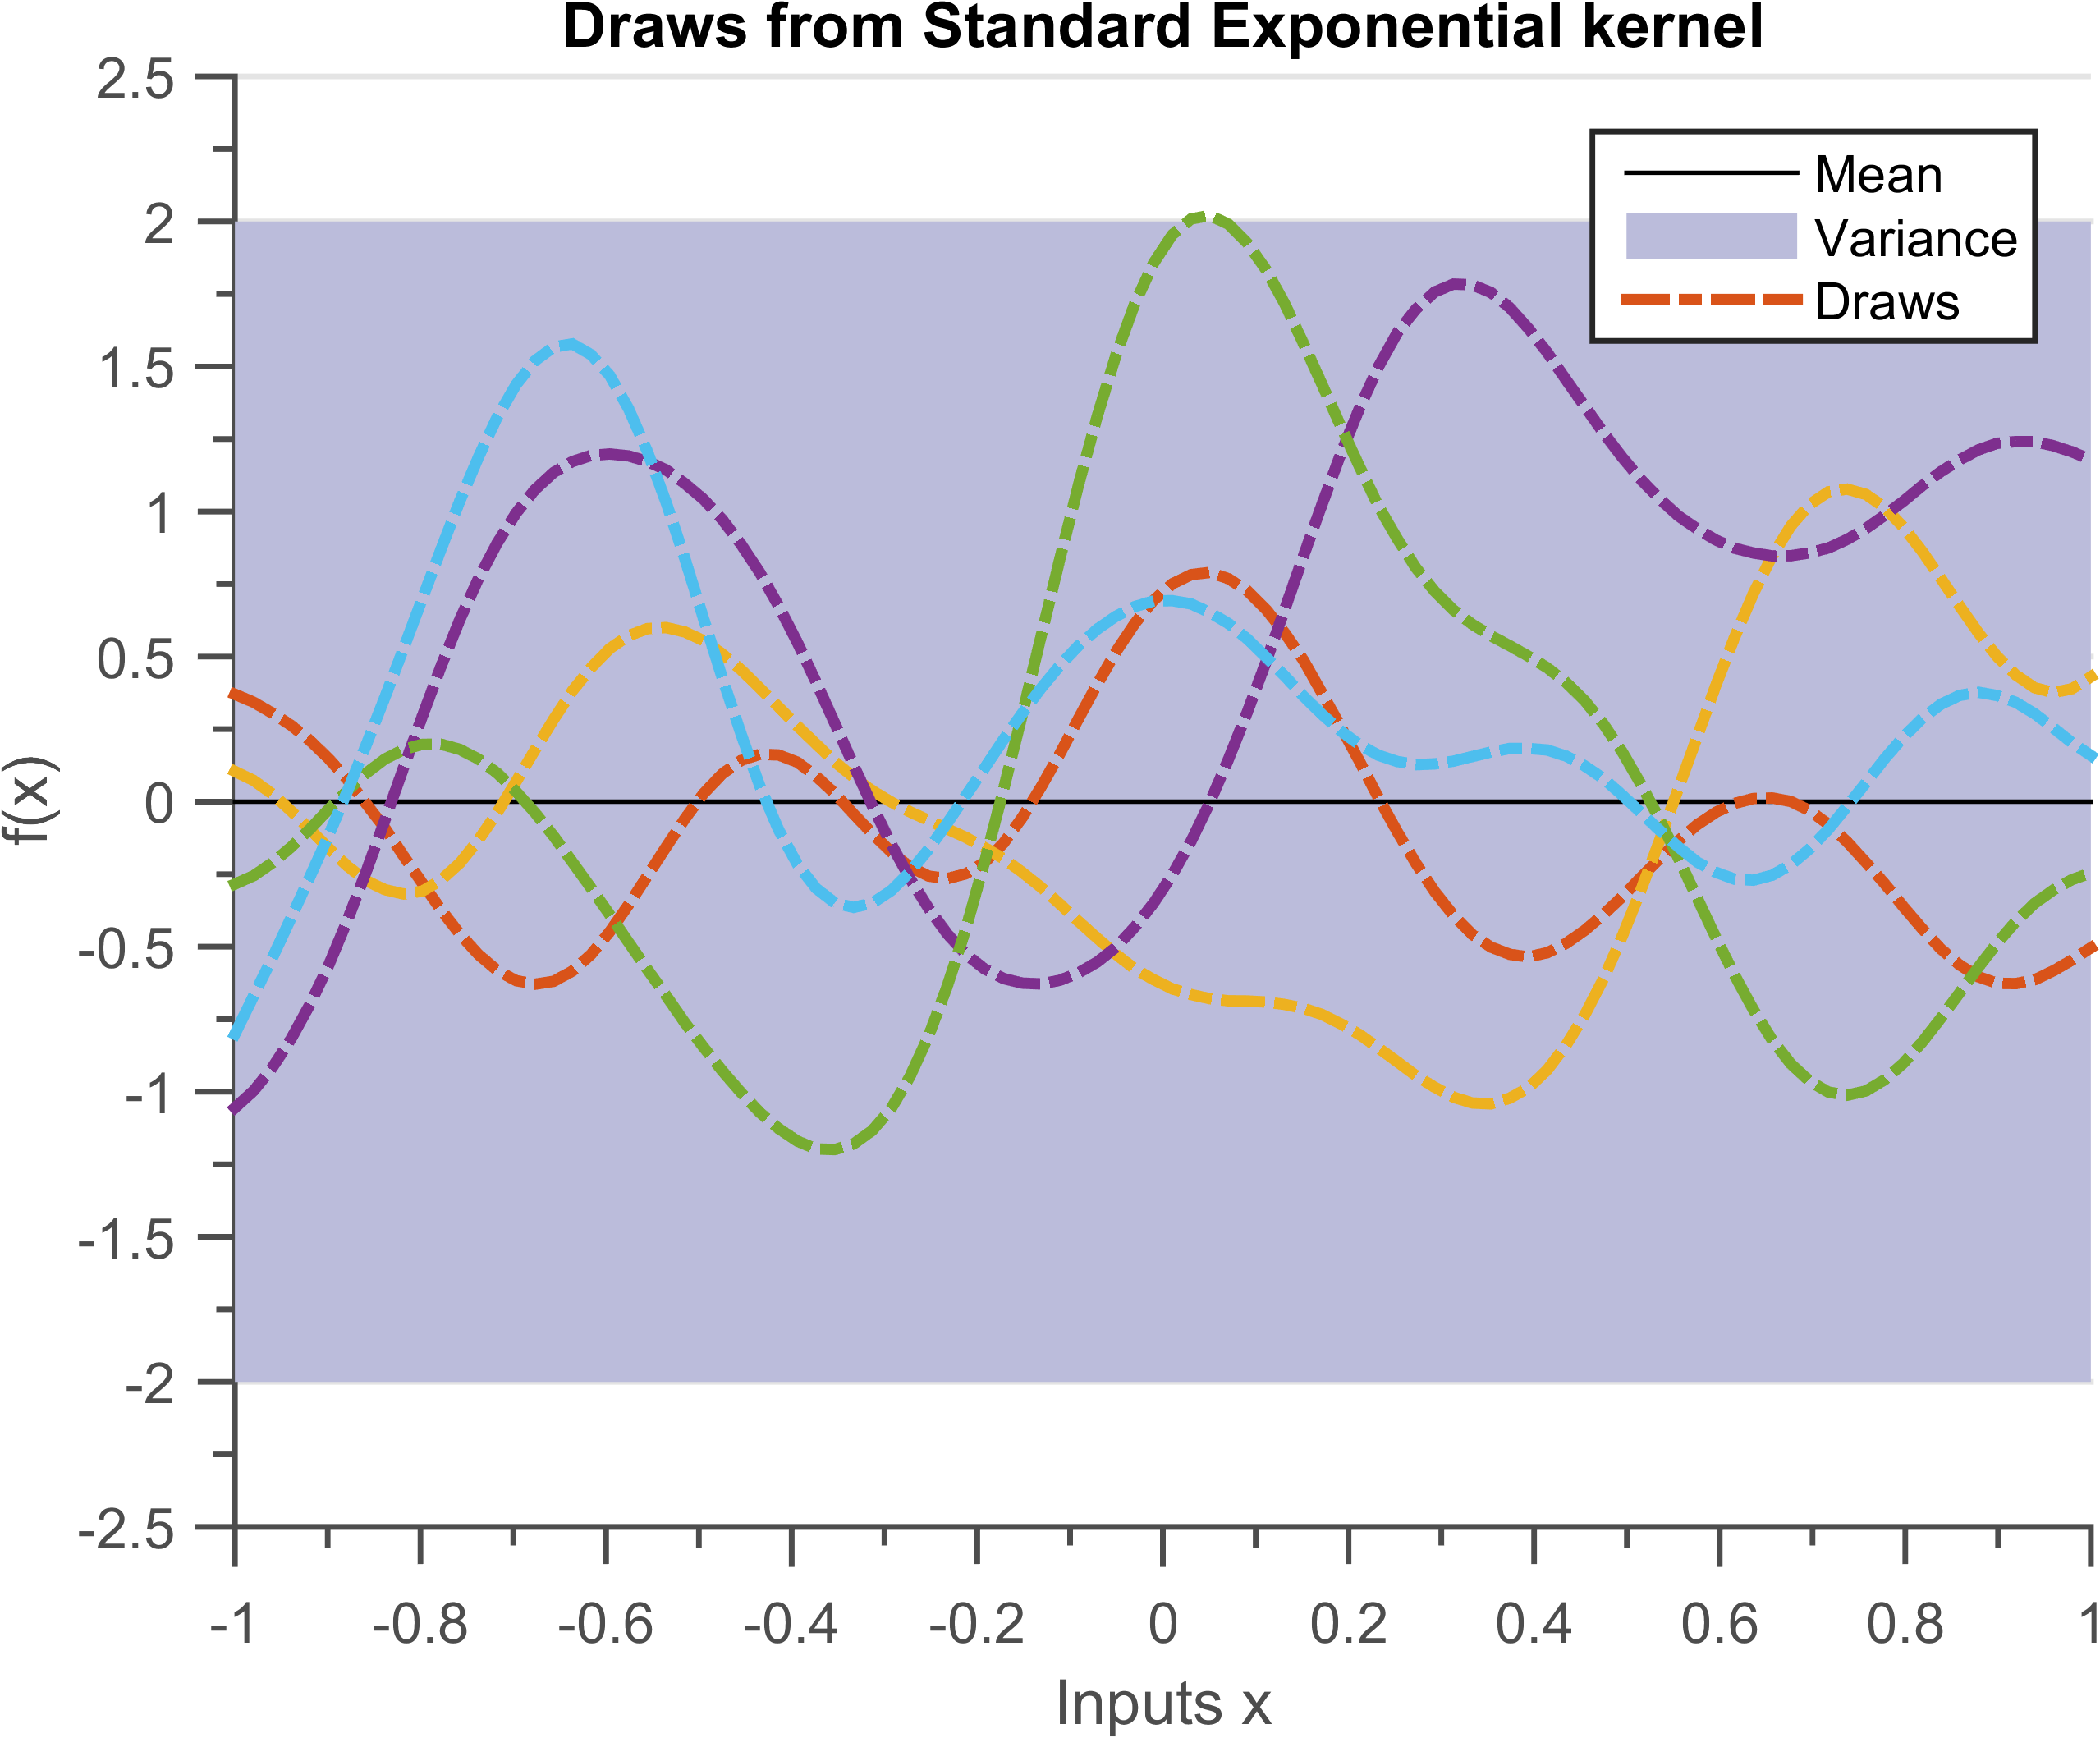
\includegraphics[width=0.45\textwidth]
        {images/part1/drawsSEKernel_1}
        \label{subFigSEPrior_1}
  }\quad
\subfigure[{Draws from a GP prior with mean zero and Standard Exponential (SE) with $(\theta = [1, 0.5])$}]
  {
        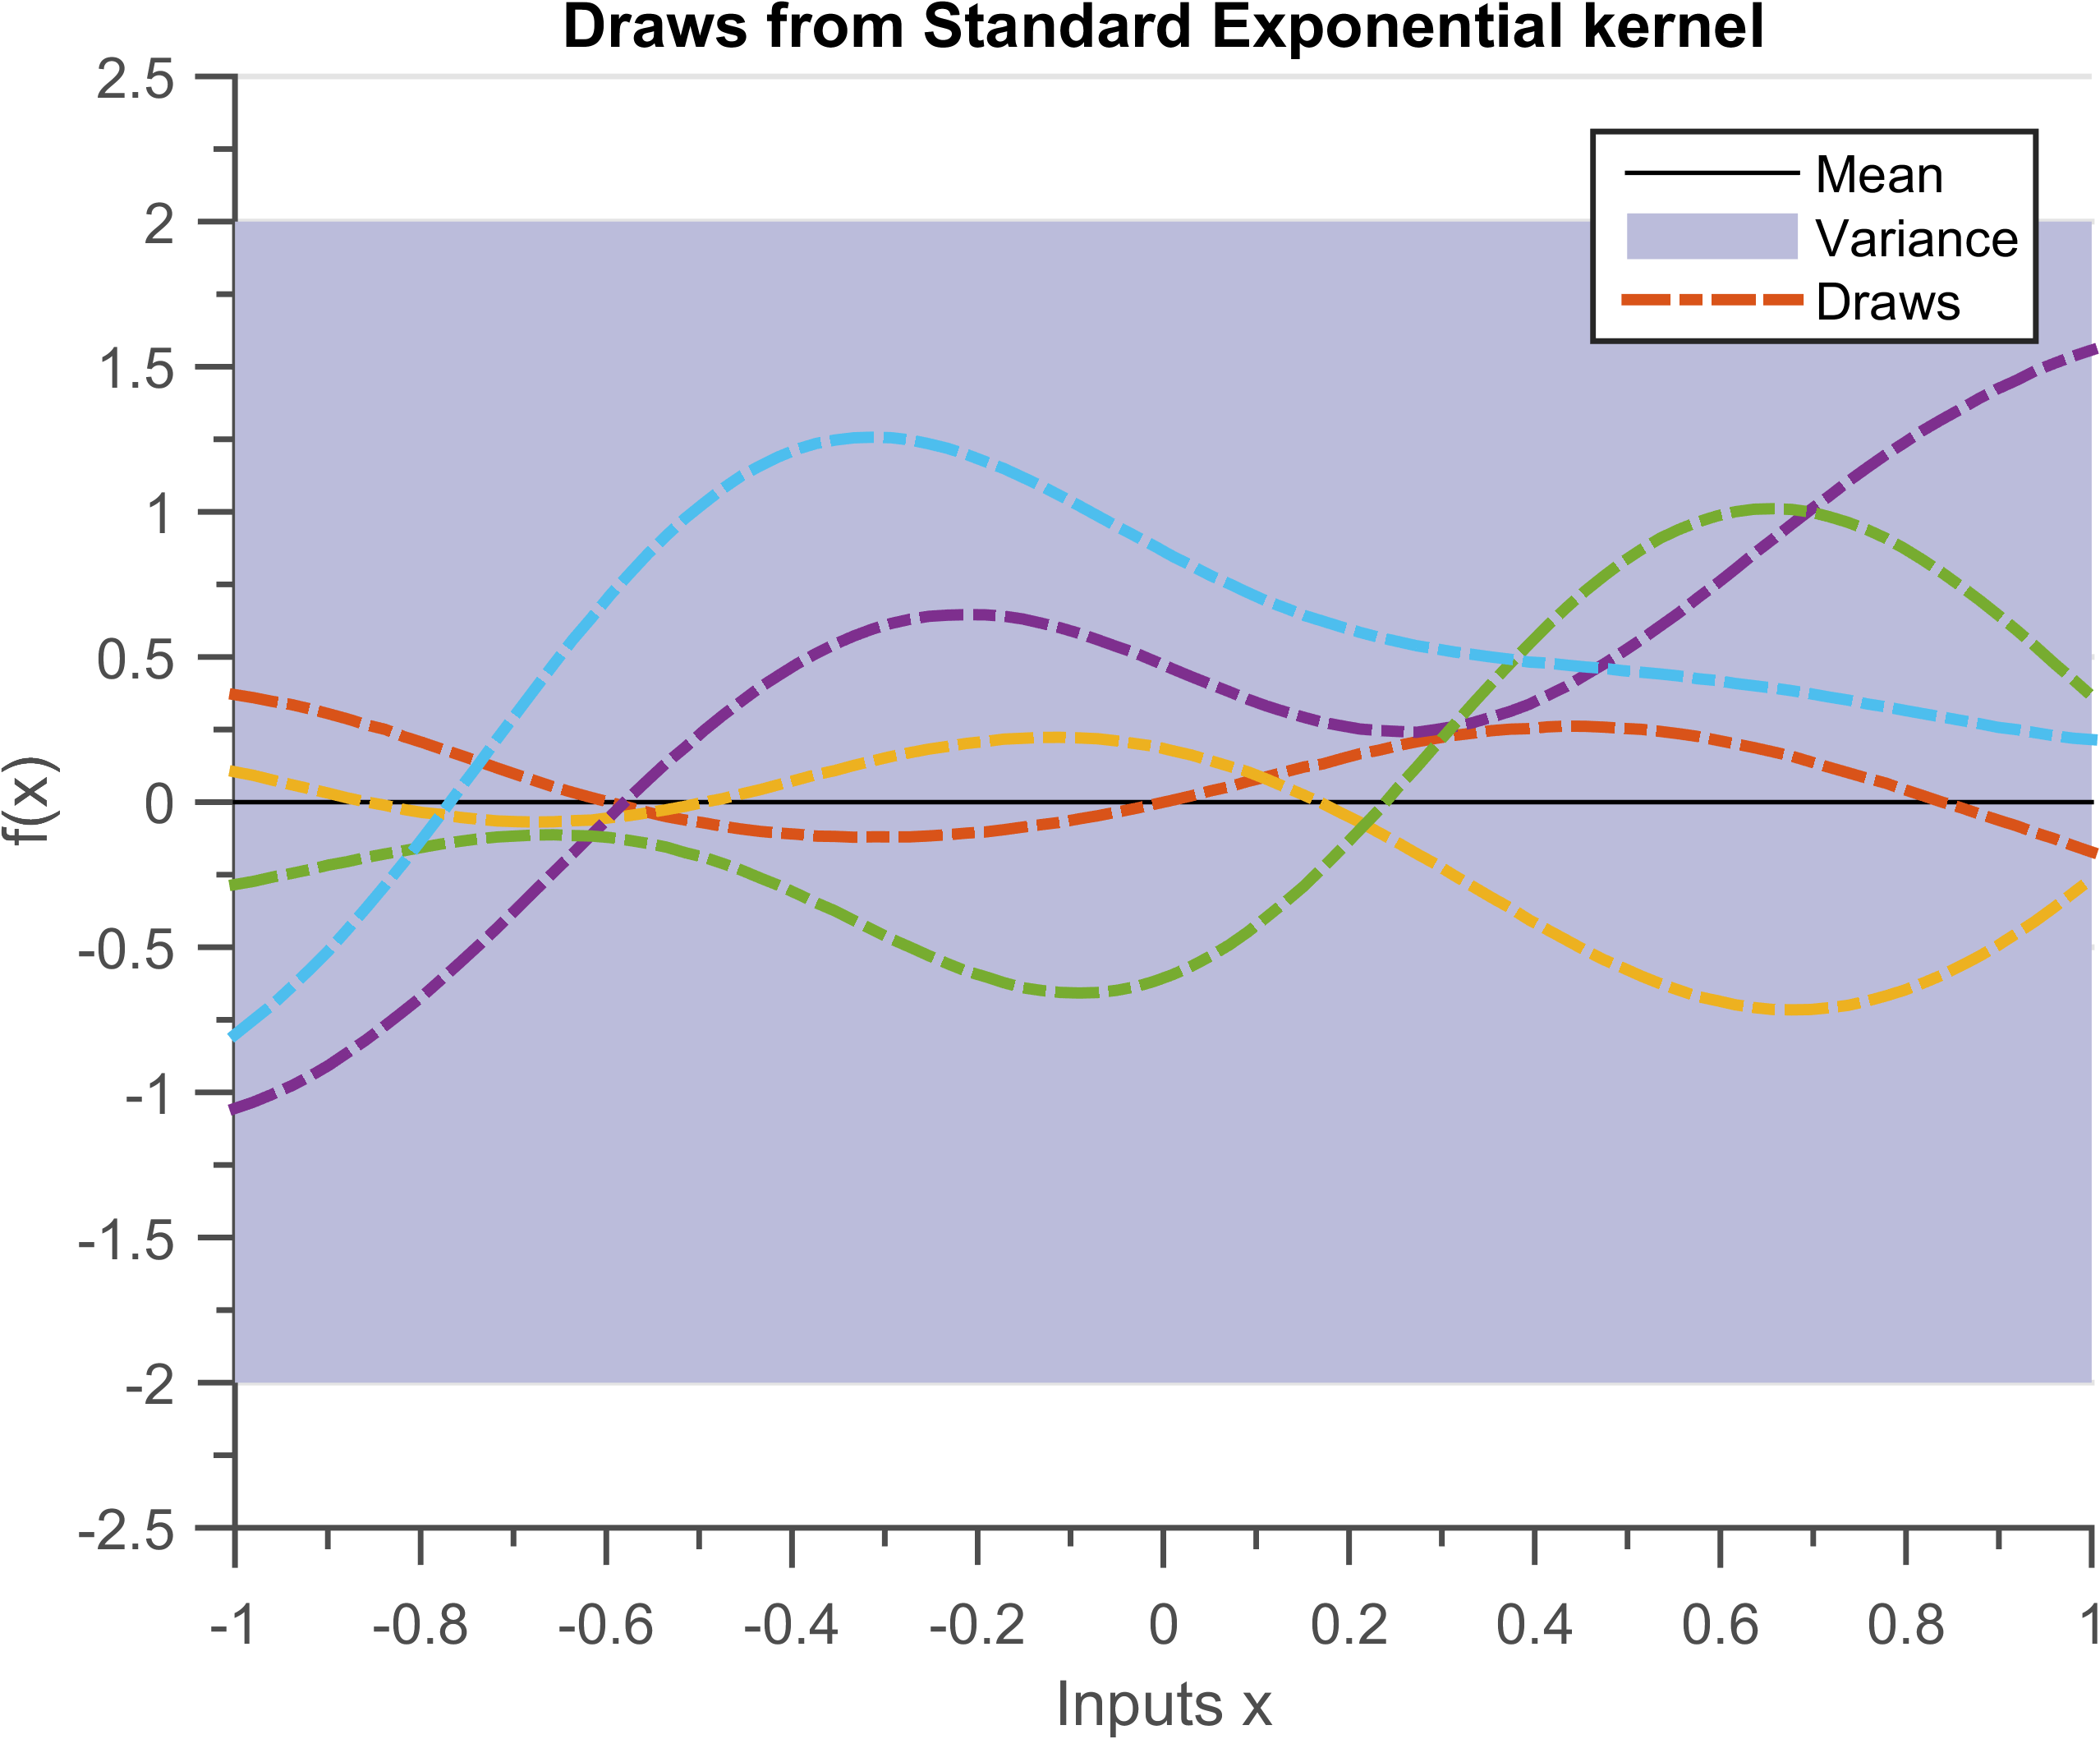
\includegraphics[width=0.45\textwidth]
        {images/part1/drawsSEKernel_2}
        \label{subFigSEPrior_2}
  }\quad
  
       \caption{The solid black line defines the mean function, shaded blue region defines 95\% confidence interval (2$\sigma$) distance away from the mean. The dashed lines are five functions drawn at random from a GP prior. We can observe that figure \ref{subFigSEPrior_1} varies faster when compared to figure \ref{subFigSEPrior_2} due to smaller length scale hyper-parameter.       }\label{figGPPriors}
\end{figure}



\section{Posterior}\label{secPosterior}
Once we have defined an appropriate prior we wish to incorporate the information of training data set into the probabilistic framework. In the Bayesian framework, a posterior is the probability distribution after updating the information of evidence into prior knowledge. 


\subsection{Posterior with Noise-free observations}\label{subSecPosteriorNoiseFree}
We first consider the case of noise-free observations, that is we know $\{y(x_{i}) = f_{i} | i \in [1; N] \}$. This is case for many high-fidelity computer simulations, since high-fidelity computer simulations can be treated as having no noise \cite{sacks1989design}. If we desire to interpolate at $N_{*}$ test points $X_{*}$, then the multi-variate distribution of the training outputs $f(X)$ and test outputs $f(X_{*})$ according to the GP prior, test and training points is given by equation \ref{equationJointPriorNoiseFree}.

\begin{equation}\label{equationJointPriorNoiseFree}
\Pr\left [ \begin{matrix}
f(X)
\\ f(X_{*})
\end{matrix} \right ] = 
\mathcal{N}\left (\left [ \begin{matrix} 0 \\ 0 \end{matrix} \right ]
, 
\left [ \begin{matrix}
K(X, X) & K(X, X_{*})\\ 
K(X_{*}, X) & K(X_{*}, X_{*})
\end{matrix} \right ]
\right)
\end{equation}

$K(X, X_{*})$ is $N \times N_{*}$ covariance matrix between the training points $X$ and test points $X_{*}$ (equation \ref{eqnCovMatrixSquaredExponential}). The other covariance matrices $K(X, X)$, $K(X_{*}, X)$ and $K(X_{*}, X_{*})$ can be computed similarly. 

The posterior will be the the conditional probability of $f(X_{*})$ given the prior and data set. For a multi-variate Gaussian the conditional distribution is also a multi-variate Gaussian and can be calculated tractably, for a more detailed derivation refer to appendix \textbf{refer to the appendix here}. Graphically, we can imagine that the Bayes theorem is removing all the functions from our prior family of functions that do not pass through the data set (figure \ref{figGPNoiseLessPosteriors}). The predicted distribution after adding the information of data set into the prior can be written as:

  \begin{equation}\label{eqNoiseFreePosteriorGP}
  \begin{aligned}
  \Pr(f(X_{*}) \mid X_{*}, X, f(X)) = GP(  & K(X_{*}, X)( K(X, X) )^{-1}f(X),   \\ 
                                & K(X_{*}, X_{*}) - K(X_{*}, X)( K(X, X) )^{-1} K(X, X_{*}))
  \end{aligned}
  \end{equation}

The term $K(X_{*}, X)( K(X, X) )^{-1}f(X)$ is the predicted mean of the posterior at the test points $X_{*}$. The term $K(X_{*}, X_{*}) - K(X_{*}, X)( K(X, X) )^{-1} K(X, X_{*})$ is the predicted covariance. 

\textbf{add description of D1 and algorithm}
\textbf{Comment about the algorithm}
% Adding the algorithm
\begin{mdframed}[hidealllines=true,backgroundcolor=lightgray!20]
\lstinputlisting[caption={Calculating and plotting the mean, the variance and a sample of the posterior}, 
                    captionpos=b, 
                    label={codePosterior}, 
                    backgroundcolor = \color{MatlabCellColour},
                    style=Matlab-editor]
                    {codes/chapter2/evaluatingAndPlottingThePosterior.m}
\end{mdframed}

Figure \ref{figGPNoiseLessPosteriors} shows the posterior GP after adding observed data into the initial prior. We can see that Bayes theorem eliminates all the functions in the prior that does not pass through the data. The solid black line defines the mean function, blue region defines 95\% confidence interval (2$\sigma$) distance away from the mean. The mean of the of the posterior distribution is also used as a point estimate for interpolation. The dashed lines are three functions drawn at random from a GP posterior. Random functions can be sampled from the posterior distribution as described in the earlier section. 


\begin{figure}[!ht]
  \centering
    \subfigure[{Posterior distribution for the case of noiseless observations. Prior is a GP with mean zero and covariance as Standard Exponential (SE) Kernel with $(\theta = [1, 0.2])$, data set is $\{x = -0.5; f = 0\}$.}]
  {
        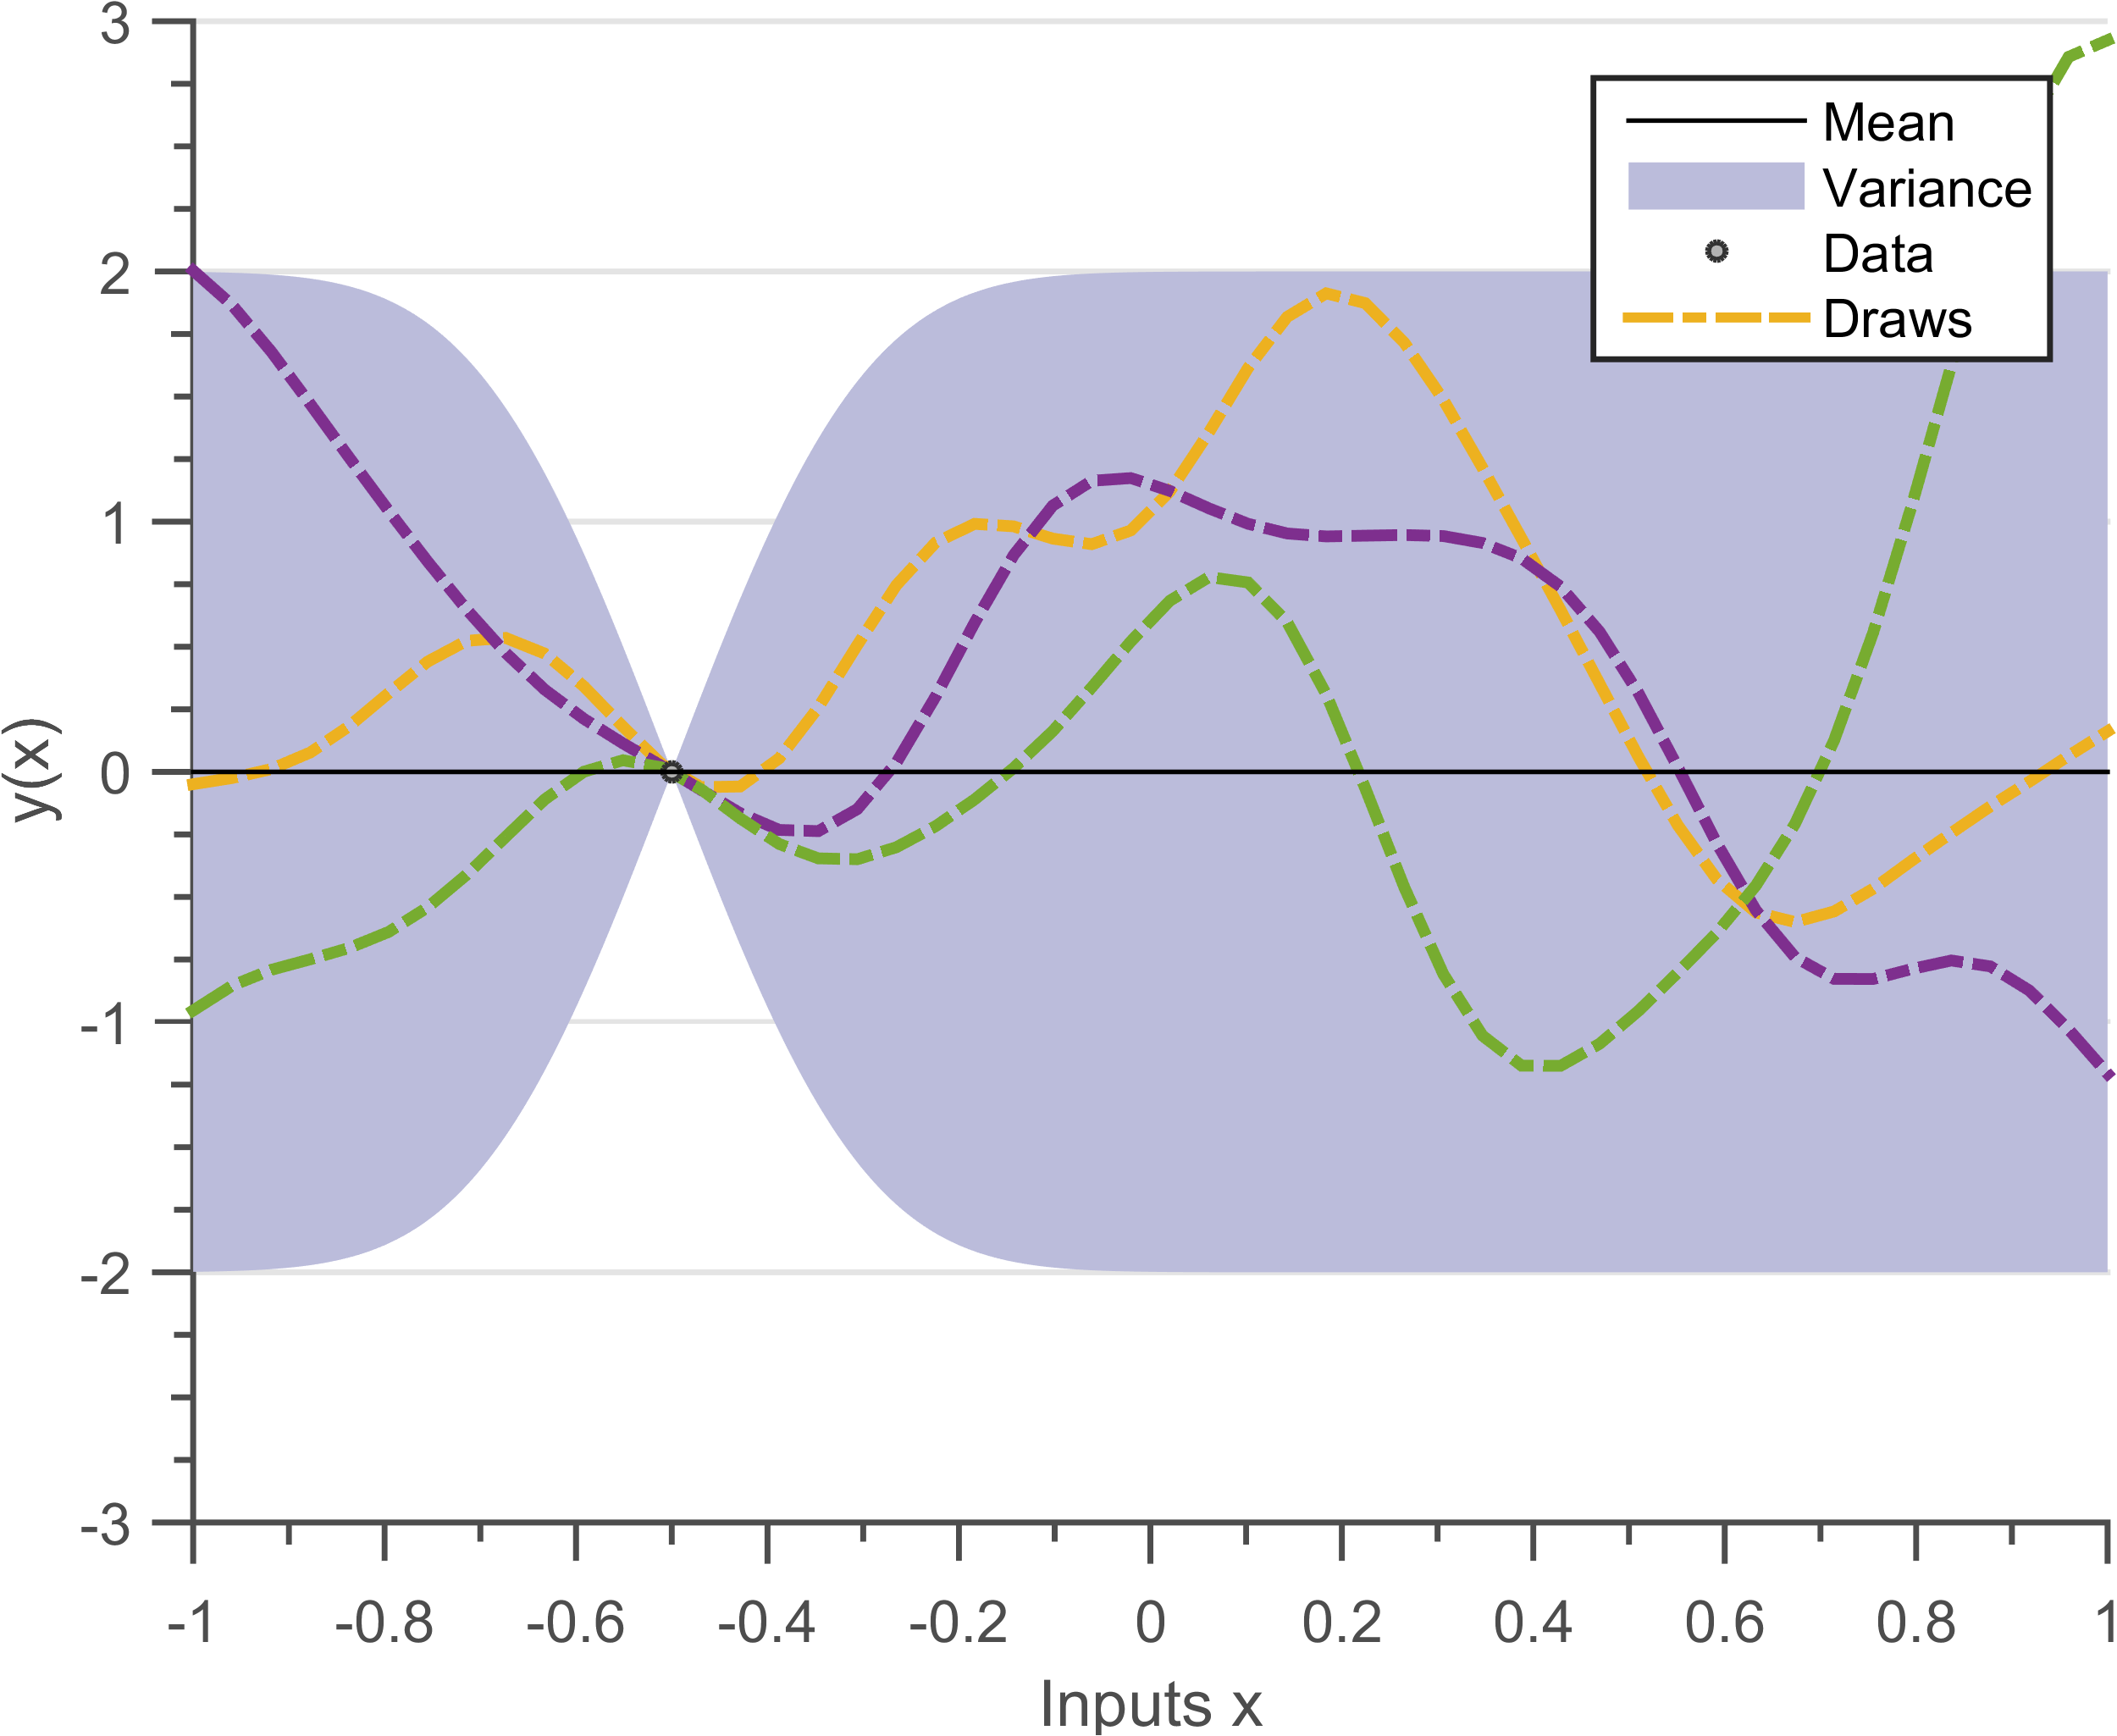
\includegraphics[width=0.45\textwidth]
        {images/part1/posteriorSENoiseLess_1}
        \label{posteriorSENoiseLess_1}
  }\quad
\subfigure[{Posterior distribution for the case of noiseless observations. Prior is a GP with mean zero and covariance as Standard Exponential (SE) Kernel with $(\theta = [1, 0.2])$, data set is $\{x = [-0.5, 0.33, 0.66]; f = [0, 0.5, 0.5]\}$}.  ]
  {
        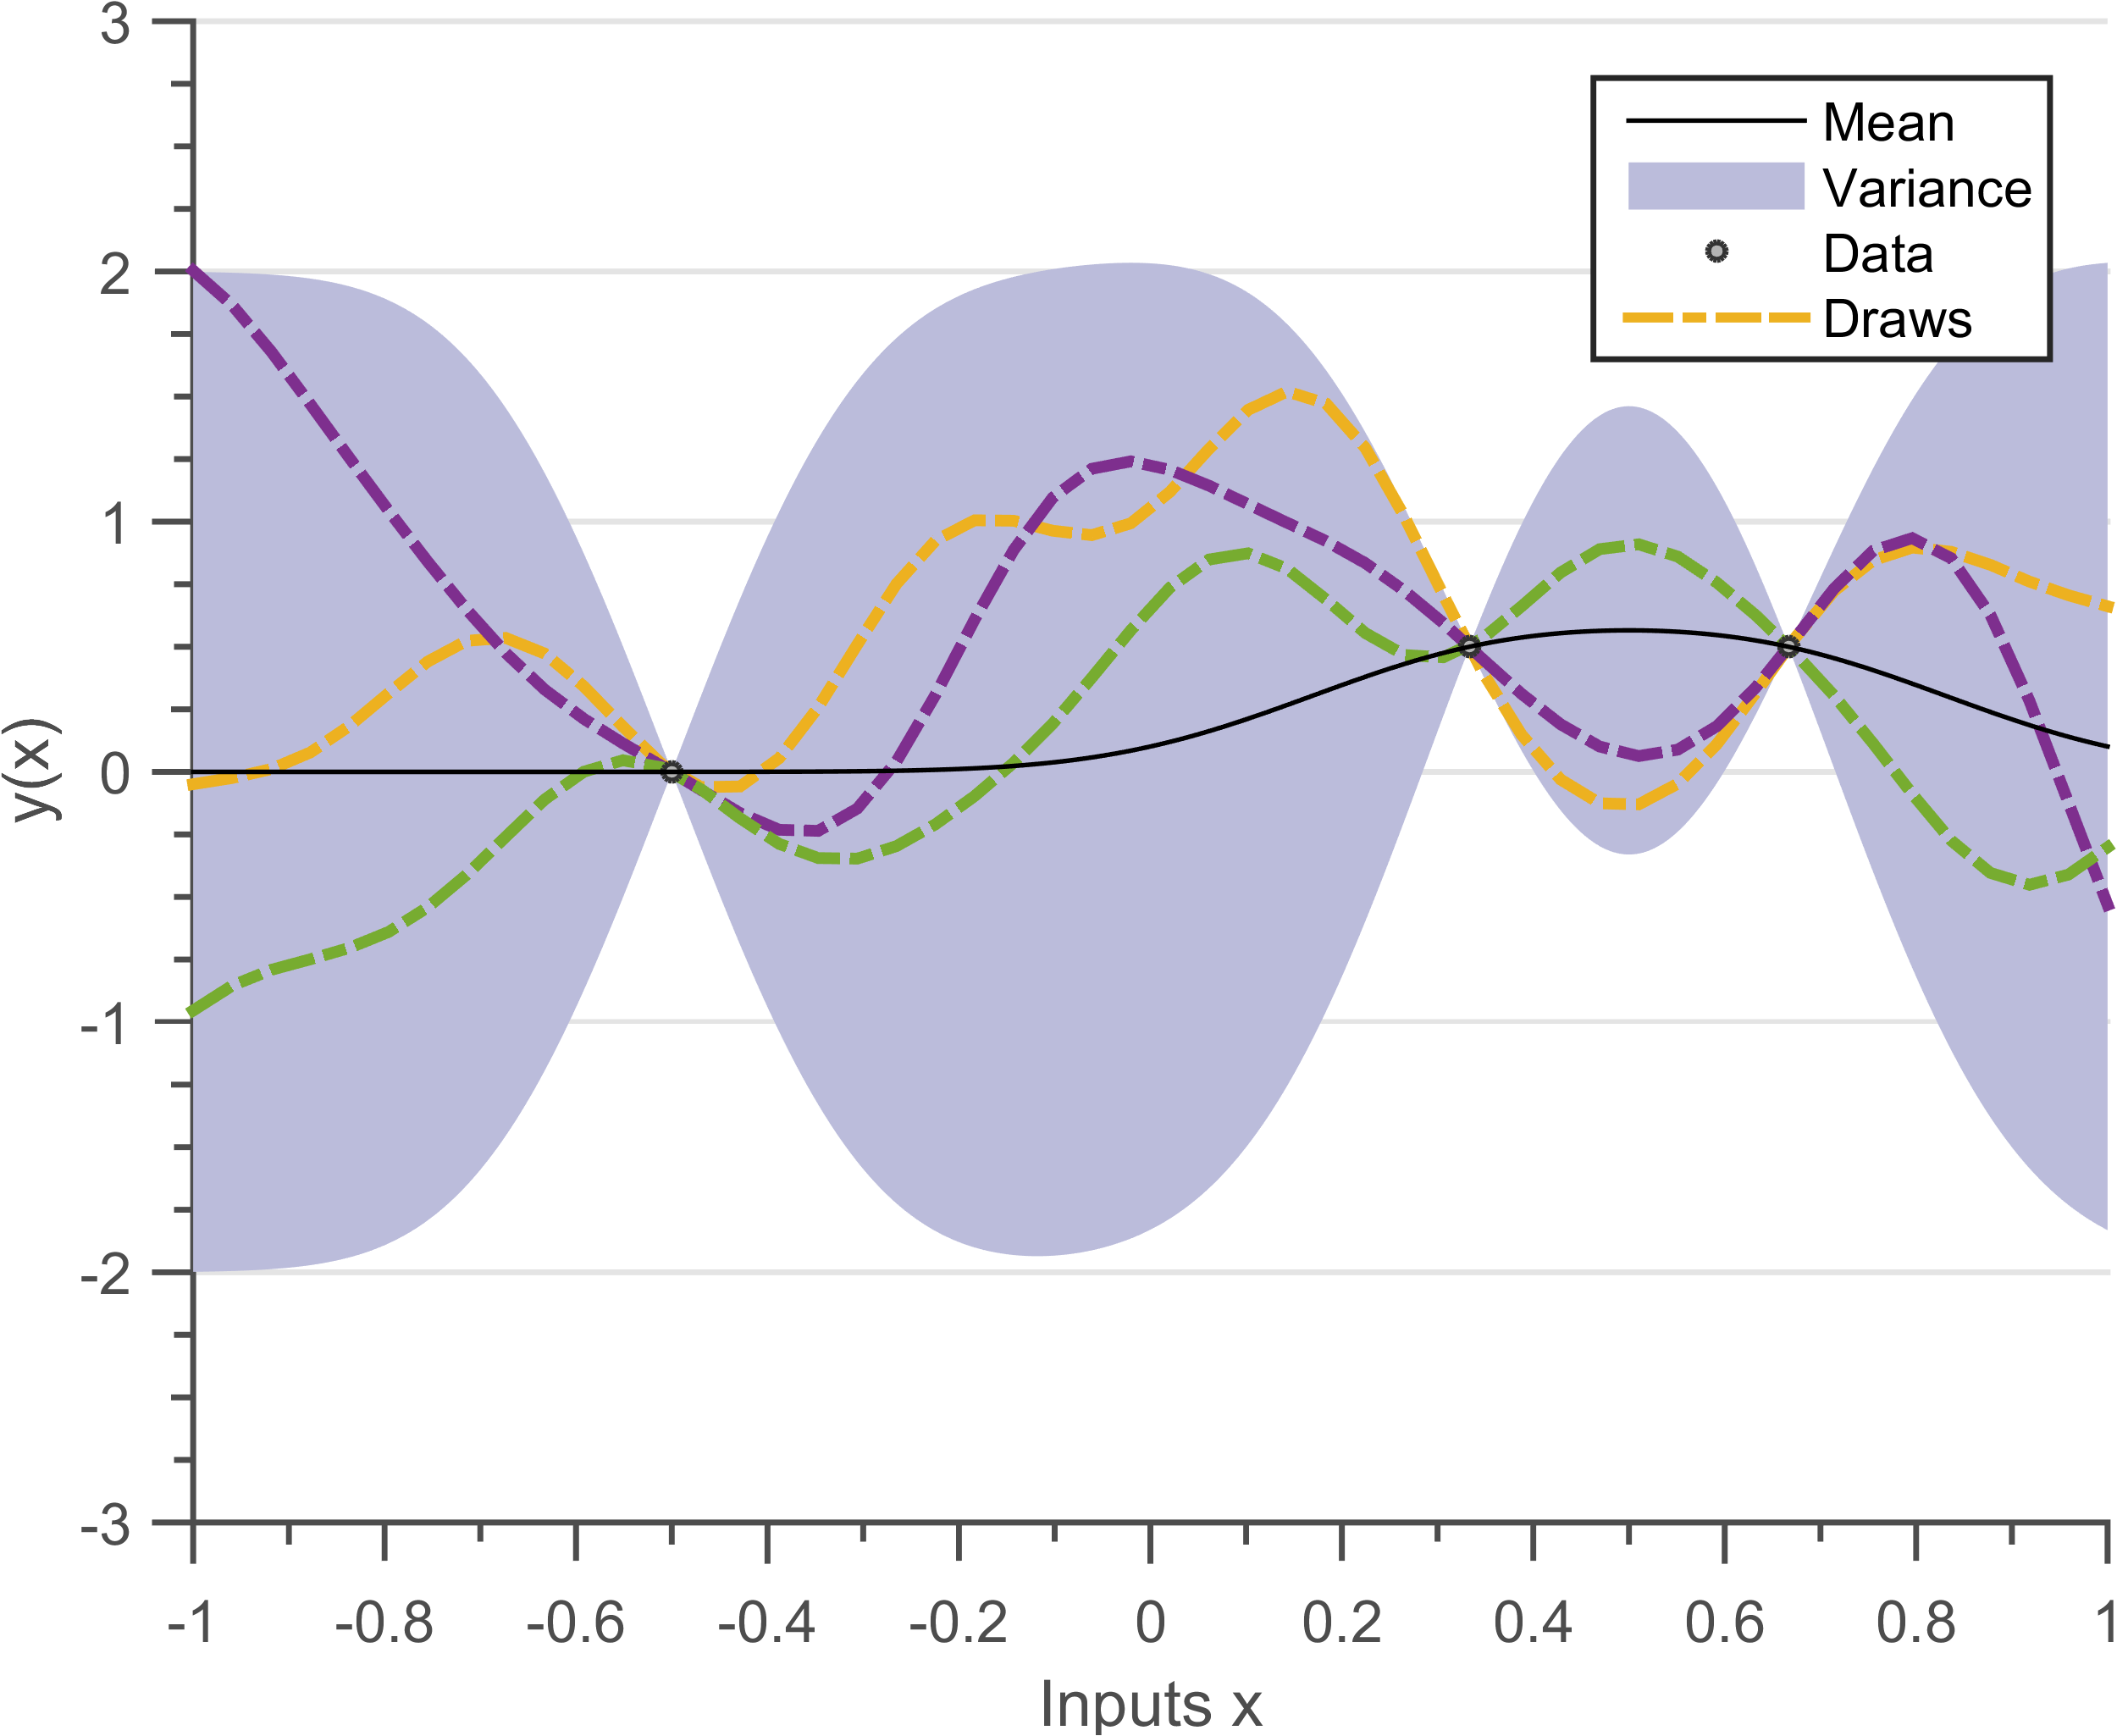
\includegraphics[width=0.45\textwidth]
        {images/part1/posteriorSENoiseLess_3}
        \label{posteriorSENoiseLess_3}
  }\quad
  
       \caption{Prediction in the case of noiseless observations. The solid black line defines the mean function, blue region defines 95\% confidence interval (2$\sigma$) distance away from the mean. The dashed lines are three functions drawn at random from a GP posterior. We can observe that Bayes Theorem eliminates all the functions that do not pass through the observed data-set.}
       \label{figGPNoiseLessPosteriors}
\end{figure}



\subsection{Posterior with Noisy observations}\label{subSecPosteriorNoisy}
If we assume a more general case of noisy observations then the measured outputs can be written as:

\begin{equation}\label{eqNoiseEquation}
y(x) = f(x) + \epsilon
\end{equation}

Such that $\epsilon$ is an independent random noise sampled from a white noise Gaussian $\mathcal{N}(0, \sigma_{n}^{2})$. We can thus write the prior GP of the noisy case as:

\begin{equation}\label{equationMeanZeroGPNoisydefinition}
\Pr[y(x) \mid X, \sigma_{n}] = GP(0 , k(x_{1}, x_{2}) + \sigma^{2}_{n}\delta_{xx'})
\end{equation}

Here, $\delta_{xx'}$ is a Kronecker delta which is one iff $x = x'$ and zero otherwise. Since the noise is independent for each observation hence there is no noise term for covariances between inputs. The joint distribution of the training outputs $Y(X)$ and true physical process $f(X_{*})$ according to the above prior becomes:

\begin{equation}\label{equationJointPriorNoisy}
\Pr\left [ \begin{matrix}
Y(X)
\\ f(X_{*})
\end{matrix} \right ]
= 
\mathcal{N}\left (
\left [ \begin{matrix}
0
\\ 0

\end{matrix} \right ] , \left [ \begin{matrix}
K(X, X) + \sigma^{2}_{n}I & K(X, X_{*})\\ 
K(X_{*}, X) & K(X_{*}, X_{*})
\end{matrix} \right ] 
\right )
\end{equation}

The difference between equation \ref{equationJointPriorNoisy} and \ref{equationJointPriorNoiseFree} is the addition of noise term $\sigma^{2}_{n}I$. The noise is assumed to be independent hence is multiplied to an identity matrix, to know how to add more complex noise models please refer to chapter \ref{chapBasicCovarianceKernels}. The posterior distribution of $f(X_{*})$ can be calculated as:

  \begin{equation}\label{eqNoisyPredictiveGP}
  \begin{aligned}
      \Pr(f(X_{*}) \mid X_{*}, X, Y(X)) = GP(  & K(X_{*}, X)( K(X, X) + \sigma^{2}_{n}I)^{-1}f(X),   \\ 
                                & K(X_{*}, X_{*}) - K(X_{*}, X)( K(X, X) + \sigma^{2}_{n}I)^{-1} K(X, X_{*}) 
  \end{aligned}
  \end{equation}

Figure \ref{figGPNoisyPosteriors} shows the posterior GP after adding observed data into the initial prior. The solid black line defines the mean function, blue region defines 95\% confidence interval (2$\sigma$) distance away from the mean. The dashed lines are three functions drawn at random from a GP posterior. Random functions can be sampled from the posterior distribution as described in the earlier section \ref{secPrior}.  Due to the inclusion of noise in the prior, we see that the draws from posterior are not necessarily passing from the observed point.

\begin{figure}[!ht]
  \centering
    \subfigure[{Posterior distribution for the case of noisy observations. Prior is a GP with mean zero, covariance as Standard Exponential (SE) Kernel with $(\theta = [1, 0.2])$ and noise as $\sigma_{n} = [0.02])$, , data set is $\{x = -0.5; f = 0\}$.}]
  {
        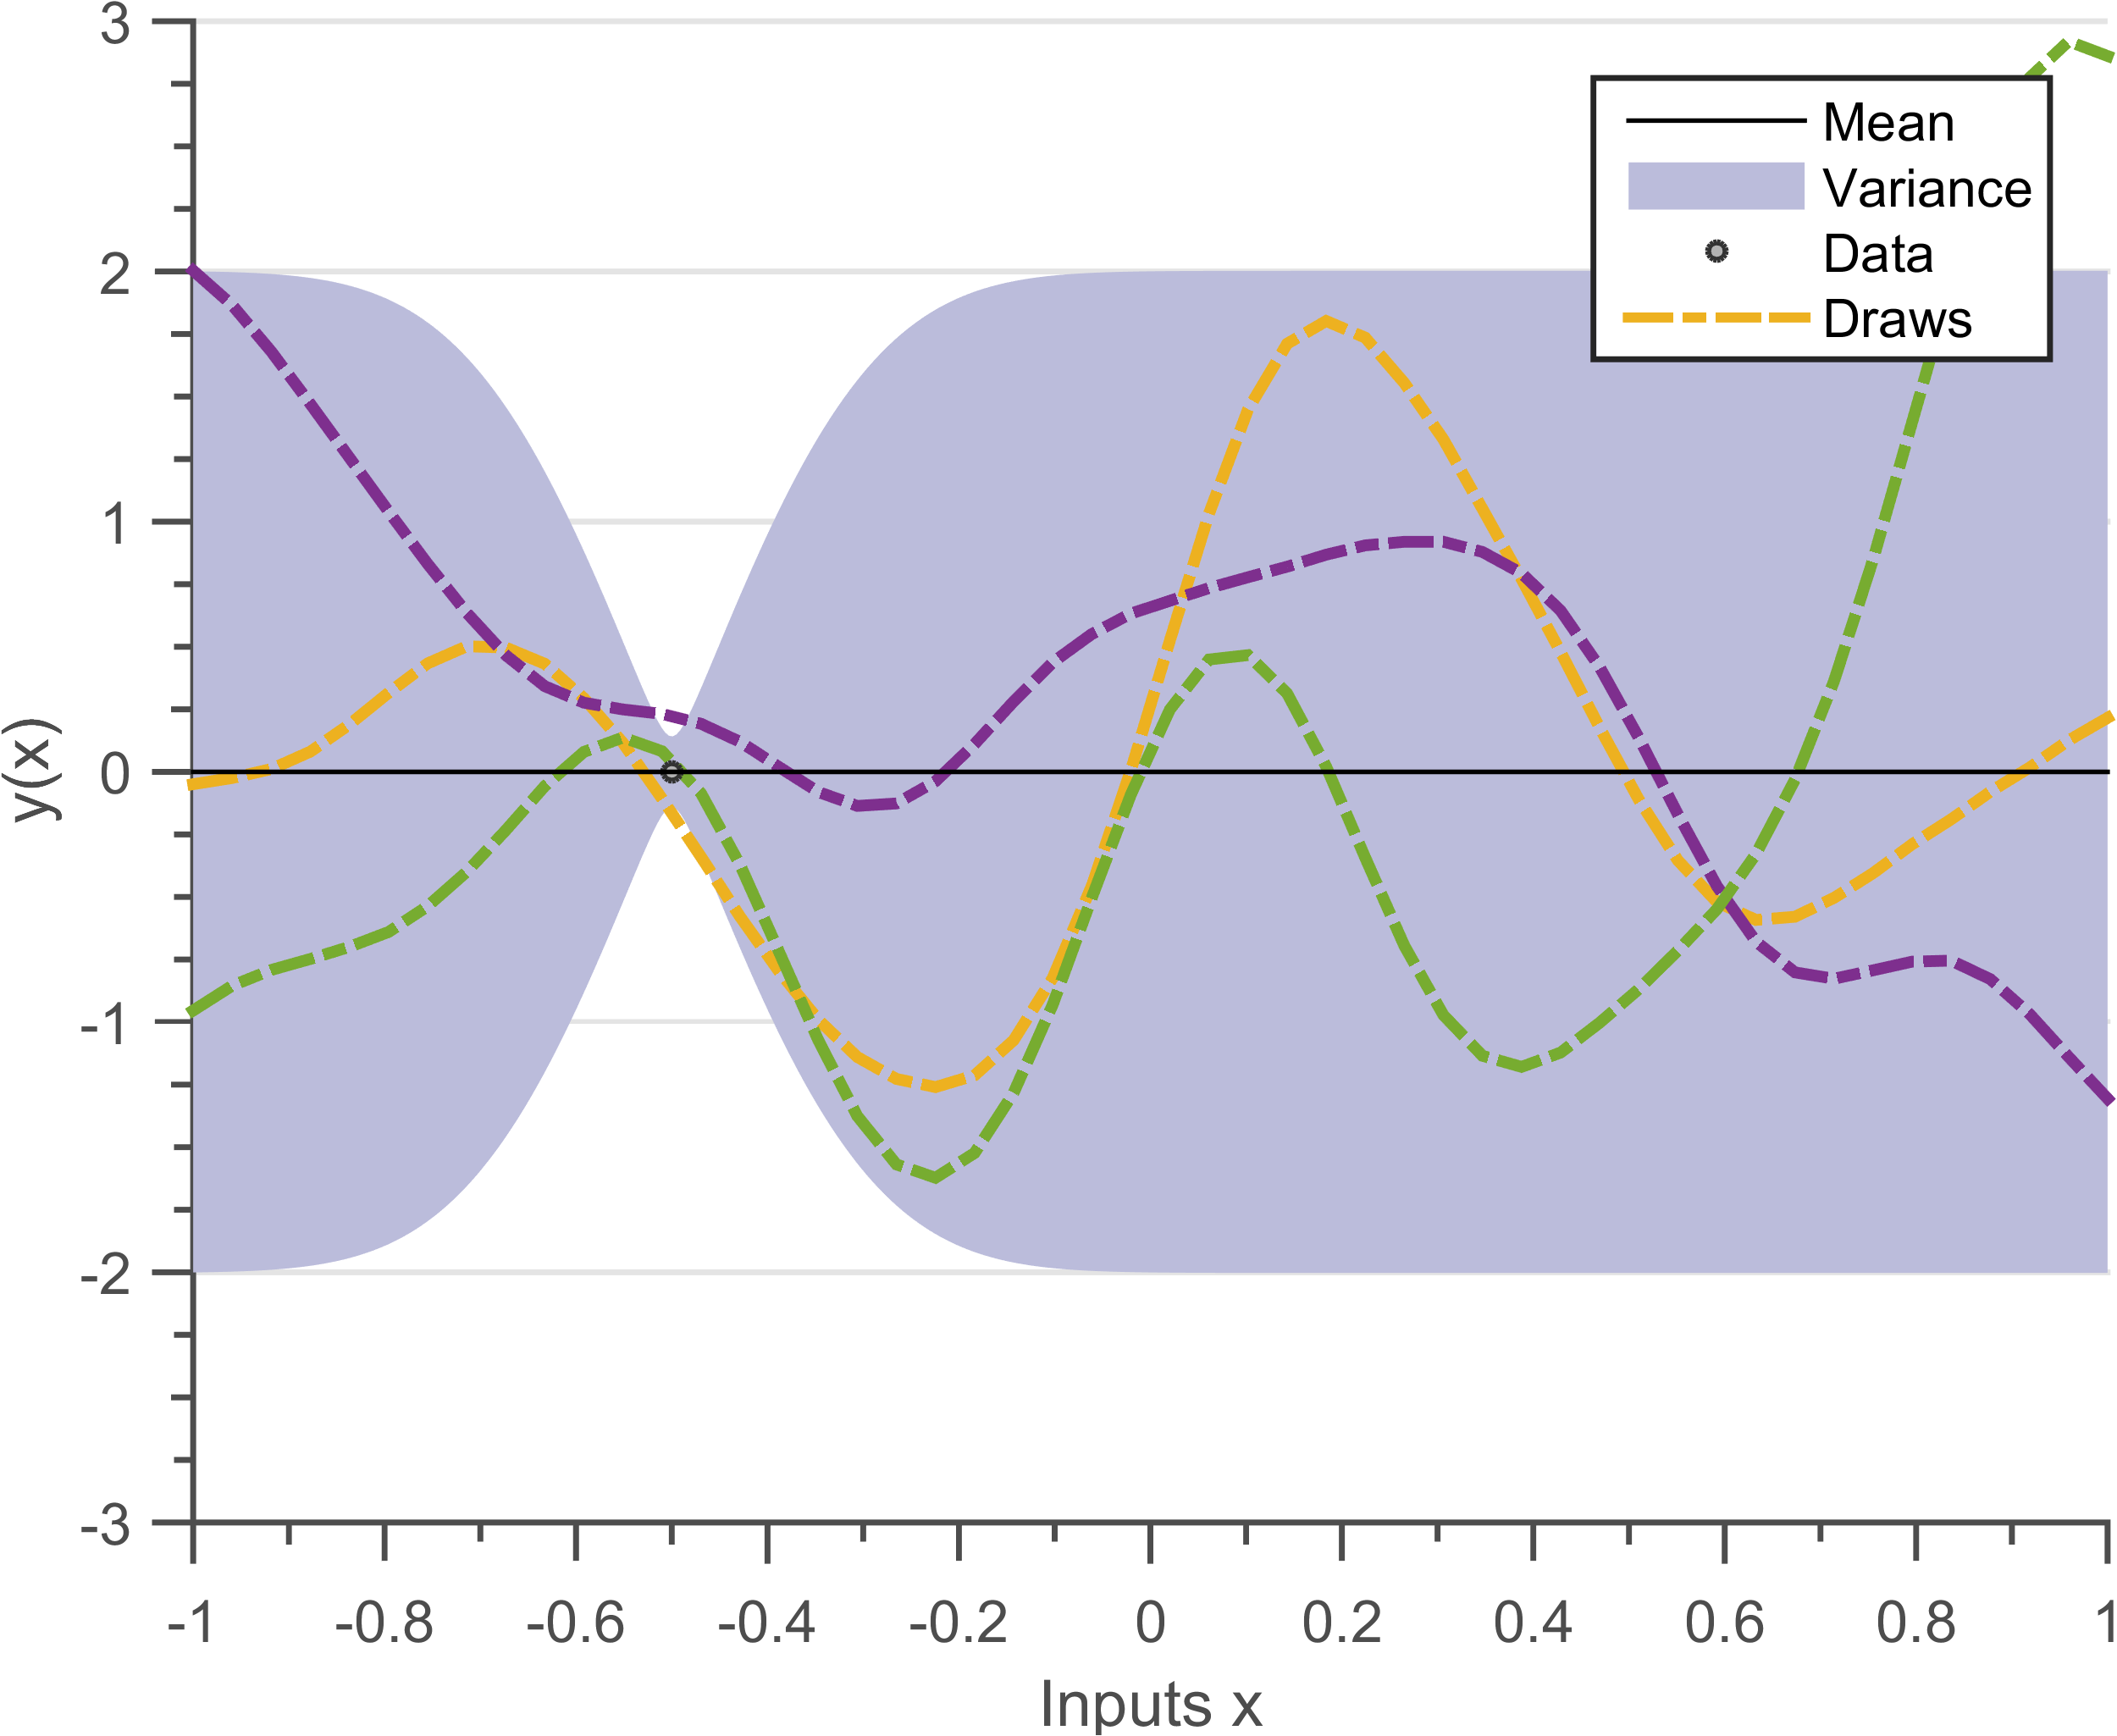
\includegraphics[width=0.45\textwidth]
        {images/part1/posteriorSENoisy_1}
        \label{posteriorSENoisy_1}
  }\quad
\subfigure[{Posterior distribution for the case of noisy observations. Prior is a GP with mean zero, covariance as Standard Exponential (SE) Kernel with $(\theta = [1, 0.2])$ and noise as $\sigma_{n} = [0.02])$, , data set is $\{x = [-0.5, 0.33, 0.66]; f = [0, 0.5, 0.5]\}$.}]
  {
        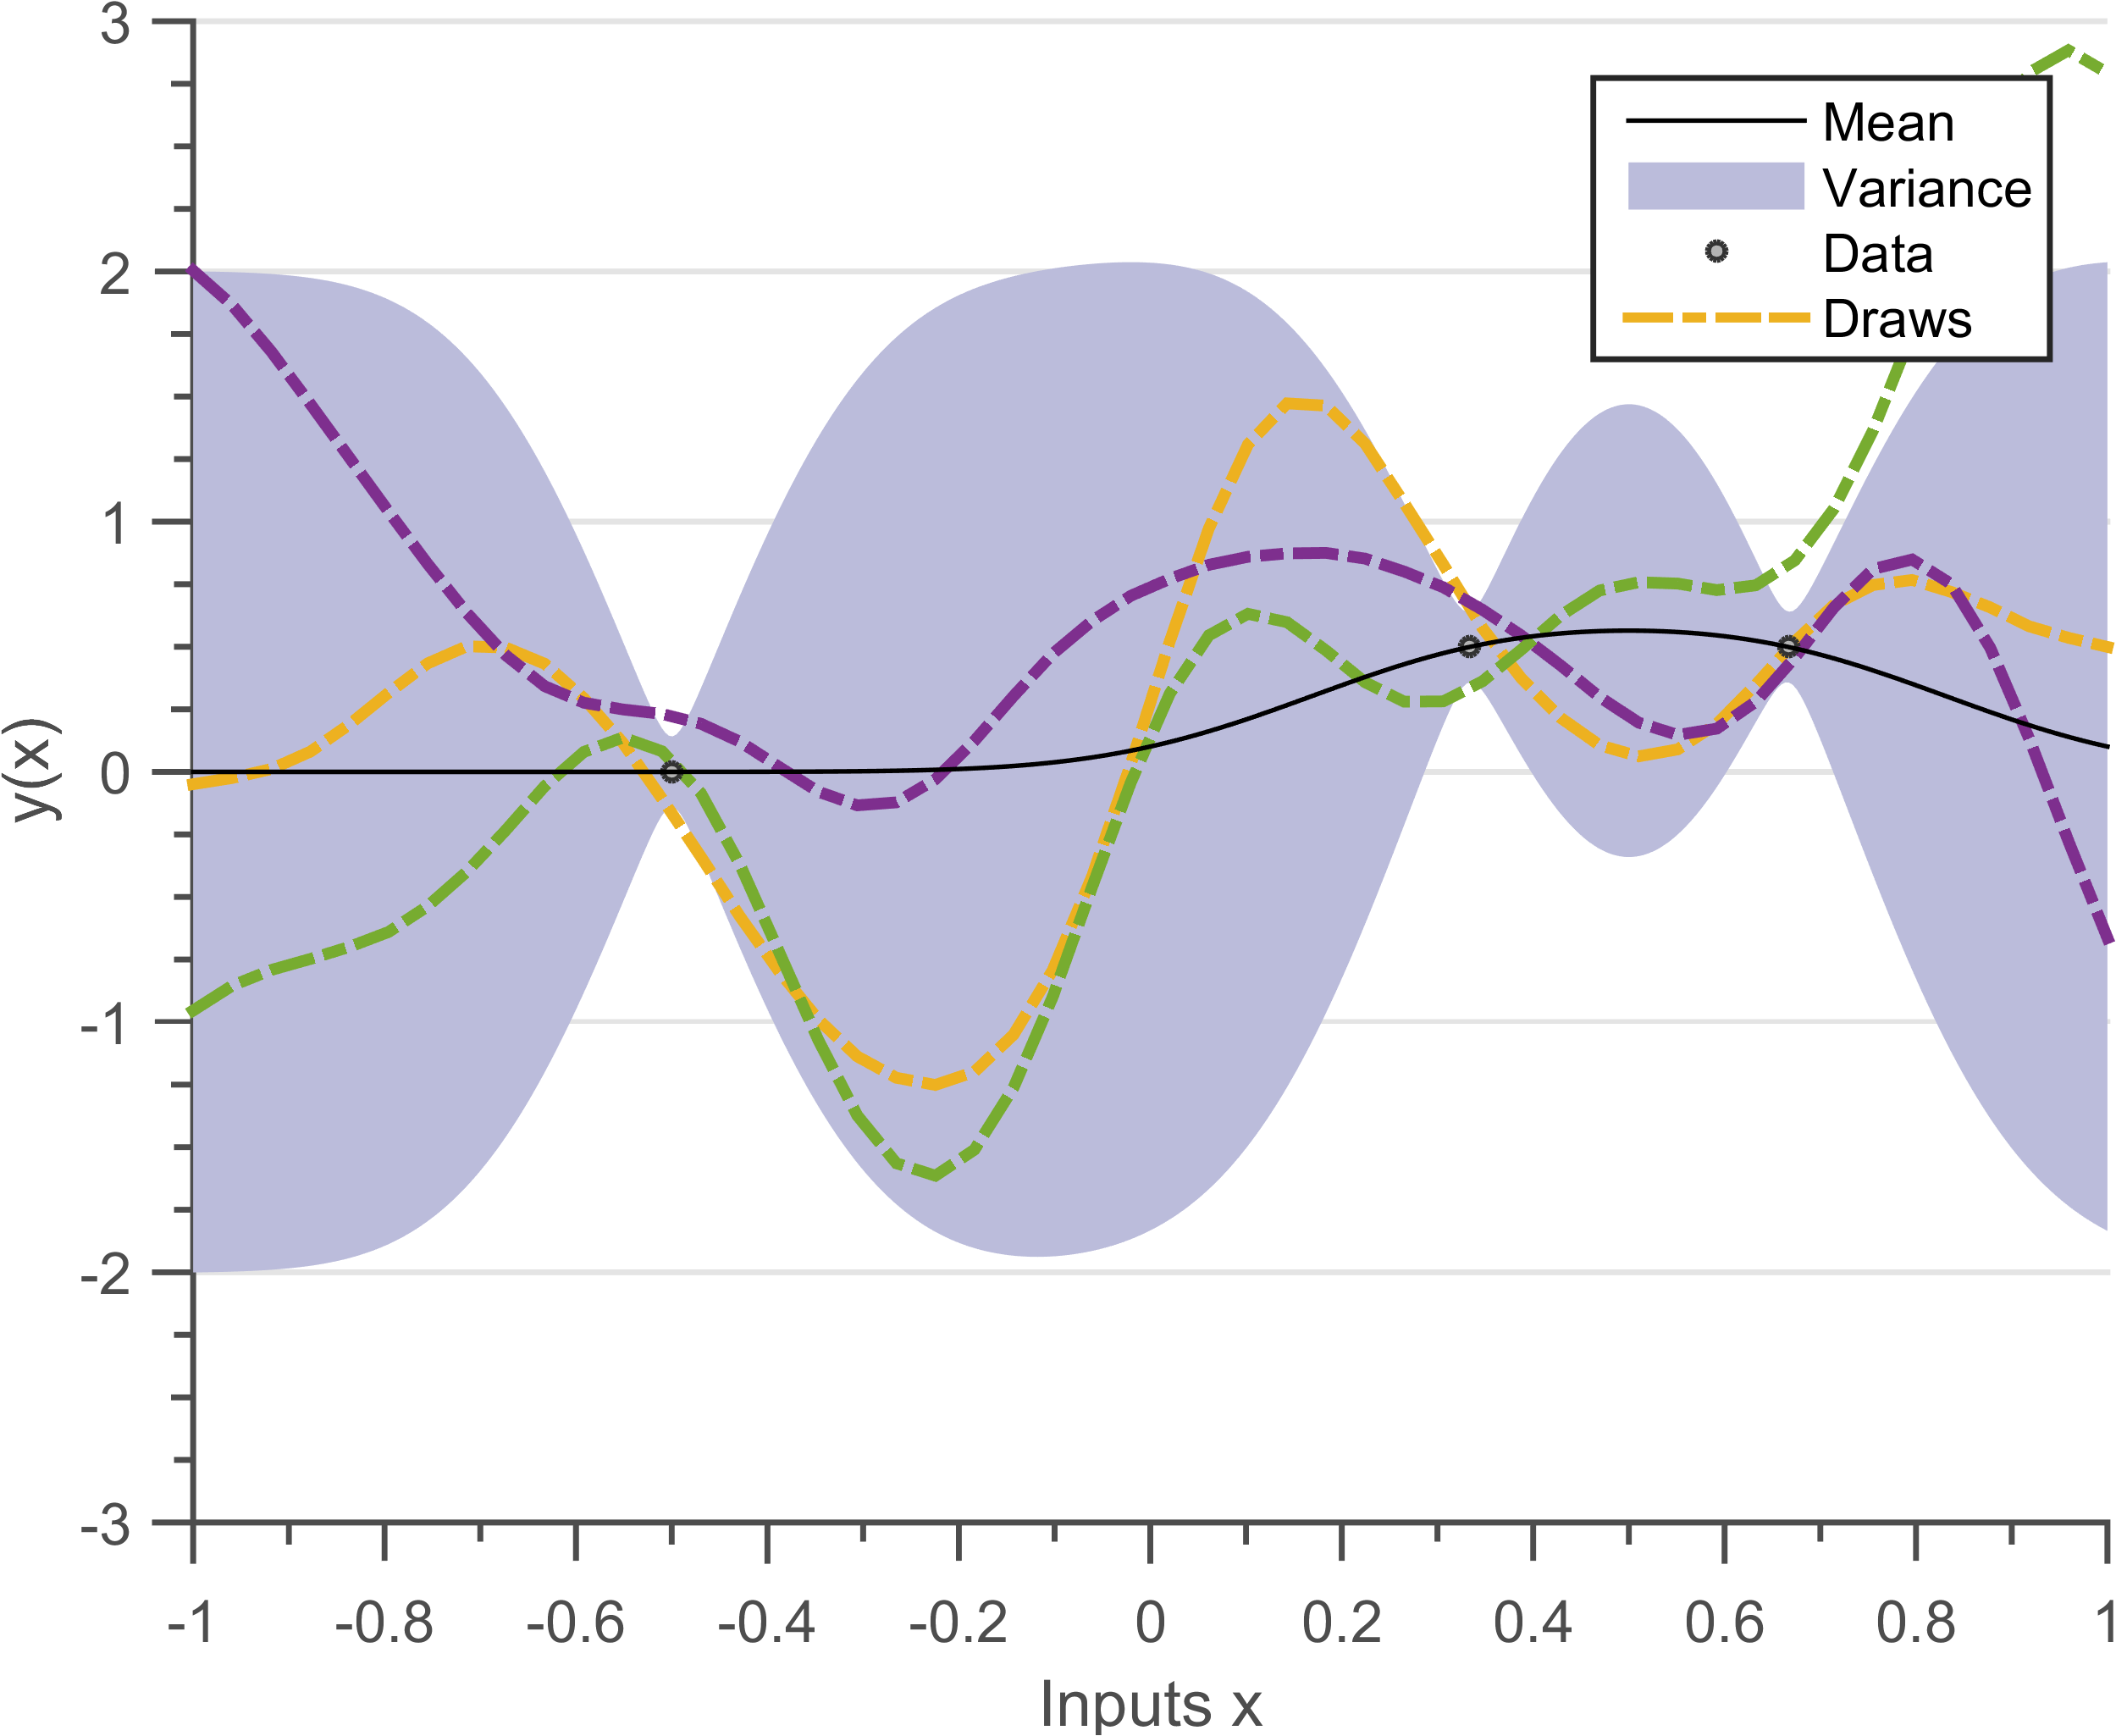
\includegraphics[width=0.45\textwidth]
        {images/part1/posteriorSENoisy_3}
        \label{posteriorSENoisy_3}
  }\quad
  
       \caption{Prediction in the case of noisy observations. The solid black line defines the mean function, blue region defines 95\% confidence interval (2$\sigma$) distance away from the mean. The dashed lines are three functions drawn at random from a GP posterior. The mean and the draws do not pass exactly from the observation point.}
       \label{figGPNoisyPosteriors}
\end{figure}

\subsection{Interpretation of posterior}
We will now introduce a short hand notation and replace the lengthy notation $K(X, X)$ with $K_{XX}$ and $K(X, X_{*})$ with $K_{XX_{*}}$. For the case when we have only one test point $x_{*}$ we can write the predictive mean and variance in short-hand as:

  \begin{equation}\label{eqNoisyPredictiveMean}
  \mathbf{E}[f(x_{*})] = K_{Xx_{*}}^{T}( K_{XX} + \sigma^{2}_{n}I)^{-1}Y
  \end{equation}
  \begin{equation}\label{eqNoisyPredictiveCovariance}
	Cov[f(x_{*})] = K_{x_{*}x_{*}} - K_{Xx_{*}}^{T}( K_{XX} + \sigma^{2}_{n}I )^{-1} K_{Xx_{*}}
  \end{equation}

\paragraph{Precision Matrix}  
Both the predictive mean (equation \ref{eqNoisyPredictiveMean}) and predictive covariance (equation \ref{eqNoisyPredictiveCovariance}) need inverse of the covariance matrix $( K_{XX} + \sigma^{2}_{n}I)^{-1}$. The inverse of a covariance matrix is also known as a precision matrix. While the elements of a covariance matrix capture the variance and correlation information, a precision matrix contains the conditional dependence information \cite{mackay2003information}. Thus, if the $(i, j)^{th}$ element of a precision matrix is zero, the $i^{th}$ and $j^{th}$ random variables are conditionally independent. 

Calculating the precision matrix is a $\mathcal{O}\left ( N^{3} \right )$ operation for a covariance matrix of size $N$. After $N \sim 10,000$ a normal computer runs out of RAM and we thus cannot perform the inversion. Fortunately, there exist several approximations to efficiently inverse the covariance matrix and perform predictions, details are available in section \ref{chapScalingGPR}.

\paragraph{Predicted mean}
The predictive mean is a linear combination of the observations $y_{i}$, and has participation-factor of $K_{Xx_{*}}^{T}( K_{XX} + \sigma^{2}_{n}I)^{-1}$. For a SE kernel $K_{Xx_{*}}^{T}$ decreases exponentially with distance, hence observations closer to $x_{*}$ have more impact on the final prediction (equation \ref{eqNoisyPredictiveMeanLinearInY}). 
  
  \begin{equation}\label{eqNoisyPredictiveMeanLinearInY}
  \mathbf{E}[f(x_{*})] = \sum_{i = 1}^{N} K_{Xx_{*}}^{T}( K_{XX} + \sigma^{2}_{n}I)^{-1}y_{i}
  \end{equation}

The predictive mean can also be interpreted as a linear combination of the basis functions $K_{x_{i}x_{*}}$, and participation factors $( K_{XX} + \sigma^{2}_{n}I)^{-1}Y$ (equation \ref{eqNoisyPredictiveMeanLinearInBasis}). 

  \begin{equation}\label{eqNoisyPredictiveMeanLinearInBasis}
  \mathbf{E}[f(x_{*})] = \sum_{i = 1}^{N} K_{x_{i}x_{*}}( K_{XX} + \sigma^{2}_{n}I)^{-1}Y
  \end{equation}
  
This means that even though a GP represents of an infinite-dimensional vector (function), we only care about the $N$ dimensional multivariate Gaussian (section \ref{equationJointPriorNoisy}) to actually predict the mean. If the precision matrix is cached, then calculating the mean is an $\mathcal{O}\left ( N \right )$ operation.

\paragraph{Predicted variance}
The predictive variance is a combination of two terms $K_{x_{*}x_{*}}$ which is the variance due to prior assumptions and $- K_{Xx_{*}}^{T}( K_{XX} + \sigma^{2}_{n}I )^{-1} K_{Xx_{*}}$ which denotes the decrease in variance due to observations. The predictive distribution of test targets $y(x_{*})$ can be calculated by adding a noise term $\sigma^{2}_{n}$ in predictive covariance equation \ref{eqNoisyPredictiveCovariance}. 

  \begin{equation}\label{eqNoisyPredictiveCovarianceOnNoisyTarget}
	Cov[y(x_{*})] = K_{x_{*}x_{*}} - K_{Xx_{*}}^{T}( K_{XX} + \sigma^{2}_{n}I )^{-1} K_{Xx_{*}} + \sigma_{n}^{2}
  \end{equation}
  
We observe that the predicted variance in not dependent on the observations $y$, this is one of the flaws in GP regression. Since the assumption that the dataset $(\mathcal{D})$ comes from a GP might not necessarily be true, the predicted variance can poorly represent the model error. Hence, predicted variance is not necessarily a measure of model error but an efficient method to track uncertainties arising from the prior assumption and non-continuous observations \cite{shah2014student}.

The mean and variance are highly dependent on the kernel hyper-parameters. In order to automatically learn the hyper-parameters, we must perform model selection. Section \ref{secHyperParameter} details how to fine-tune hyper-parameters to find an optimal prediction.

\section{Choosing Hyper-parameters}\label{secHyperParameter}
Since the properties of functions under a GP are controlled by the functional form of the covariance kernel and its hyper-parameters, model selection amounts to choosing a functional form and learning the hyper-parameters $\theta$ from data. In this section we discuss how to select an optimal model by tuning hyper-parameters for a given covariance function. Please refer to chapter \ref{chapAddingEquationsInGP} for discussion on how to choose covariance functions. 

\textbf{Comment about the code}
\begin{mdframed}[hidealllines=true,backgroundcolor=lightgray!20]
\begin{lstlisting}[caption={Code for dataset D2}, 
                    captionpos=b, 
                    label={codeDatasetD2},
                    style=Matlab-editor, 
                    backgroundcolor = \color{MatlabCellColour}]
nData = 20; % number of data points

f = @(x)sin(5*pi*x)./(5*pi*x); % Function

noise = 0.1; % Noise in dataset
xData = linspace(-1, 1, nData)';
yData = f(xData) + noise*2*rand(nData, 1);

\end{lstlisting}
\end{mdframed}

Figure \ref{figGPRMarginal} demonstrates that choosing optimal hyper-parameters is very vital for accurate prediction. Figure  \ref{figGPRMarginal} compares the posterior distributions obtained for SE priors with 2 different hyper-parameters. We observe that the mean of figure \ref{subFigPosterior1} passes through all the observed data points but is more complex. The mean in figure \ref{subFigPosterior3} is a smooth function but does not fit the data properly. 

  \begin{figure}[!ht]
  \centering
    \subfigure[{Posterior between SE prior with hyper-parameters $(\theta = [0.35, 0.05]; \sigma_{noise} = 0.01)$ and data. }]
    %$\log (ML) = -35.3$]
  {
        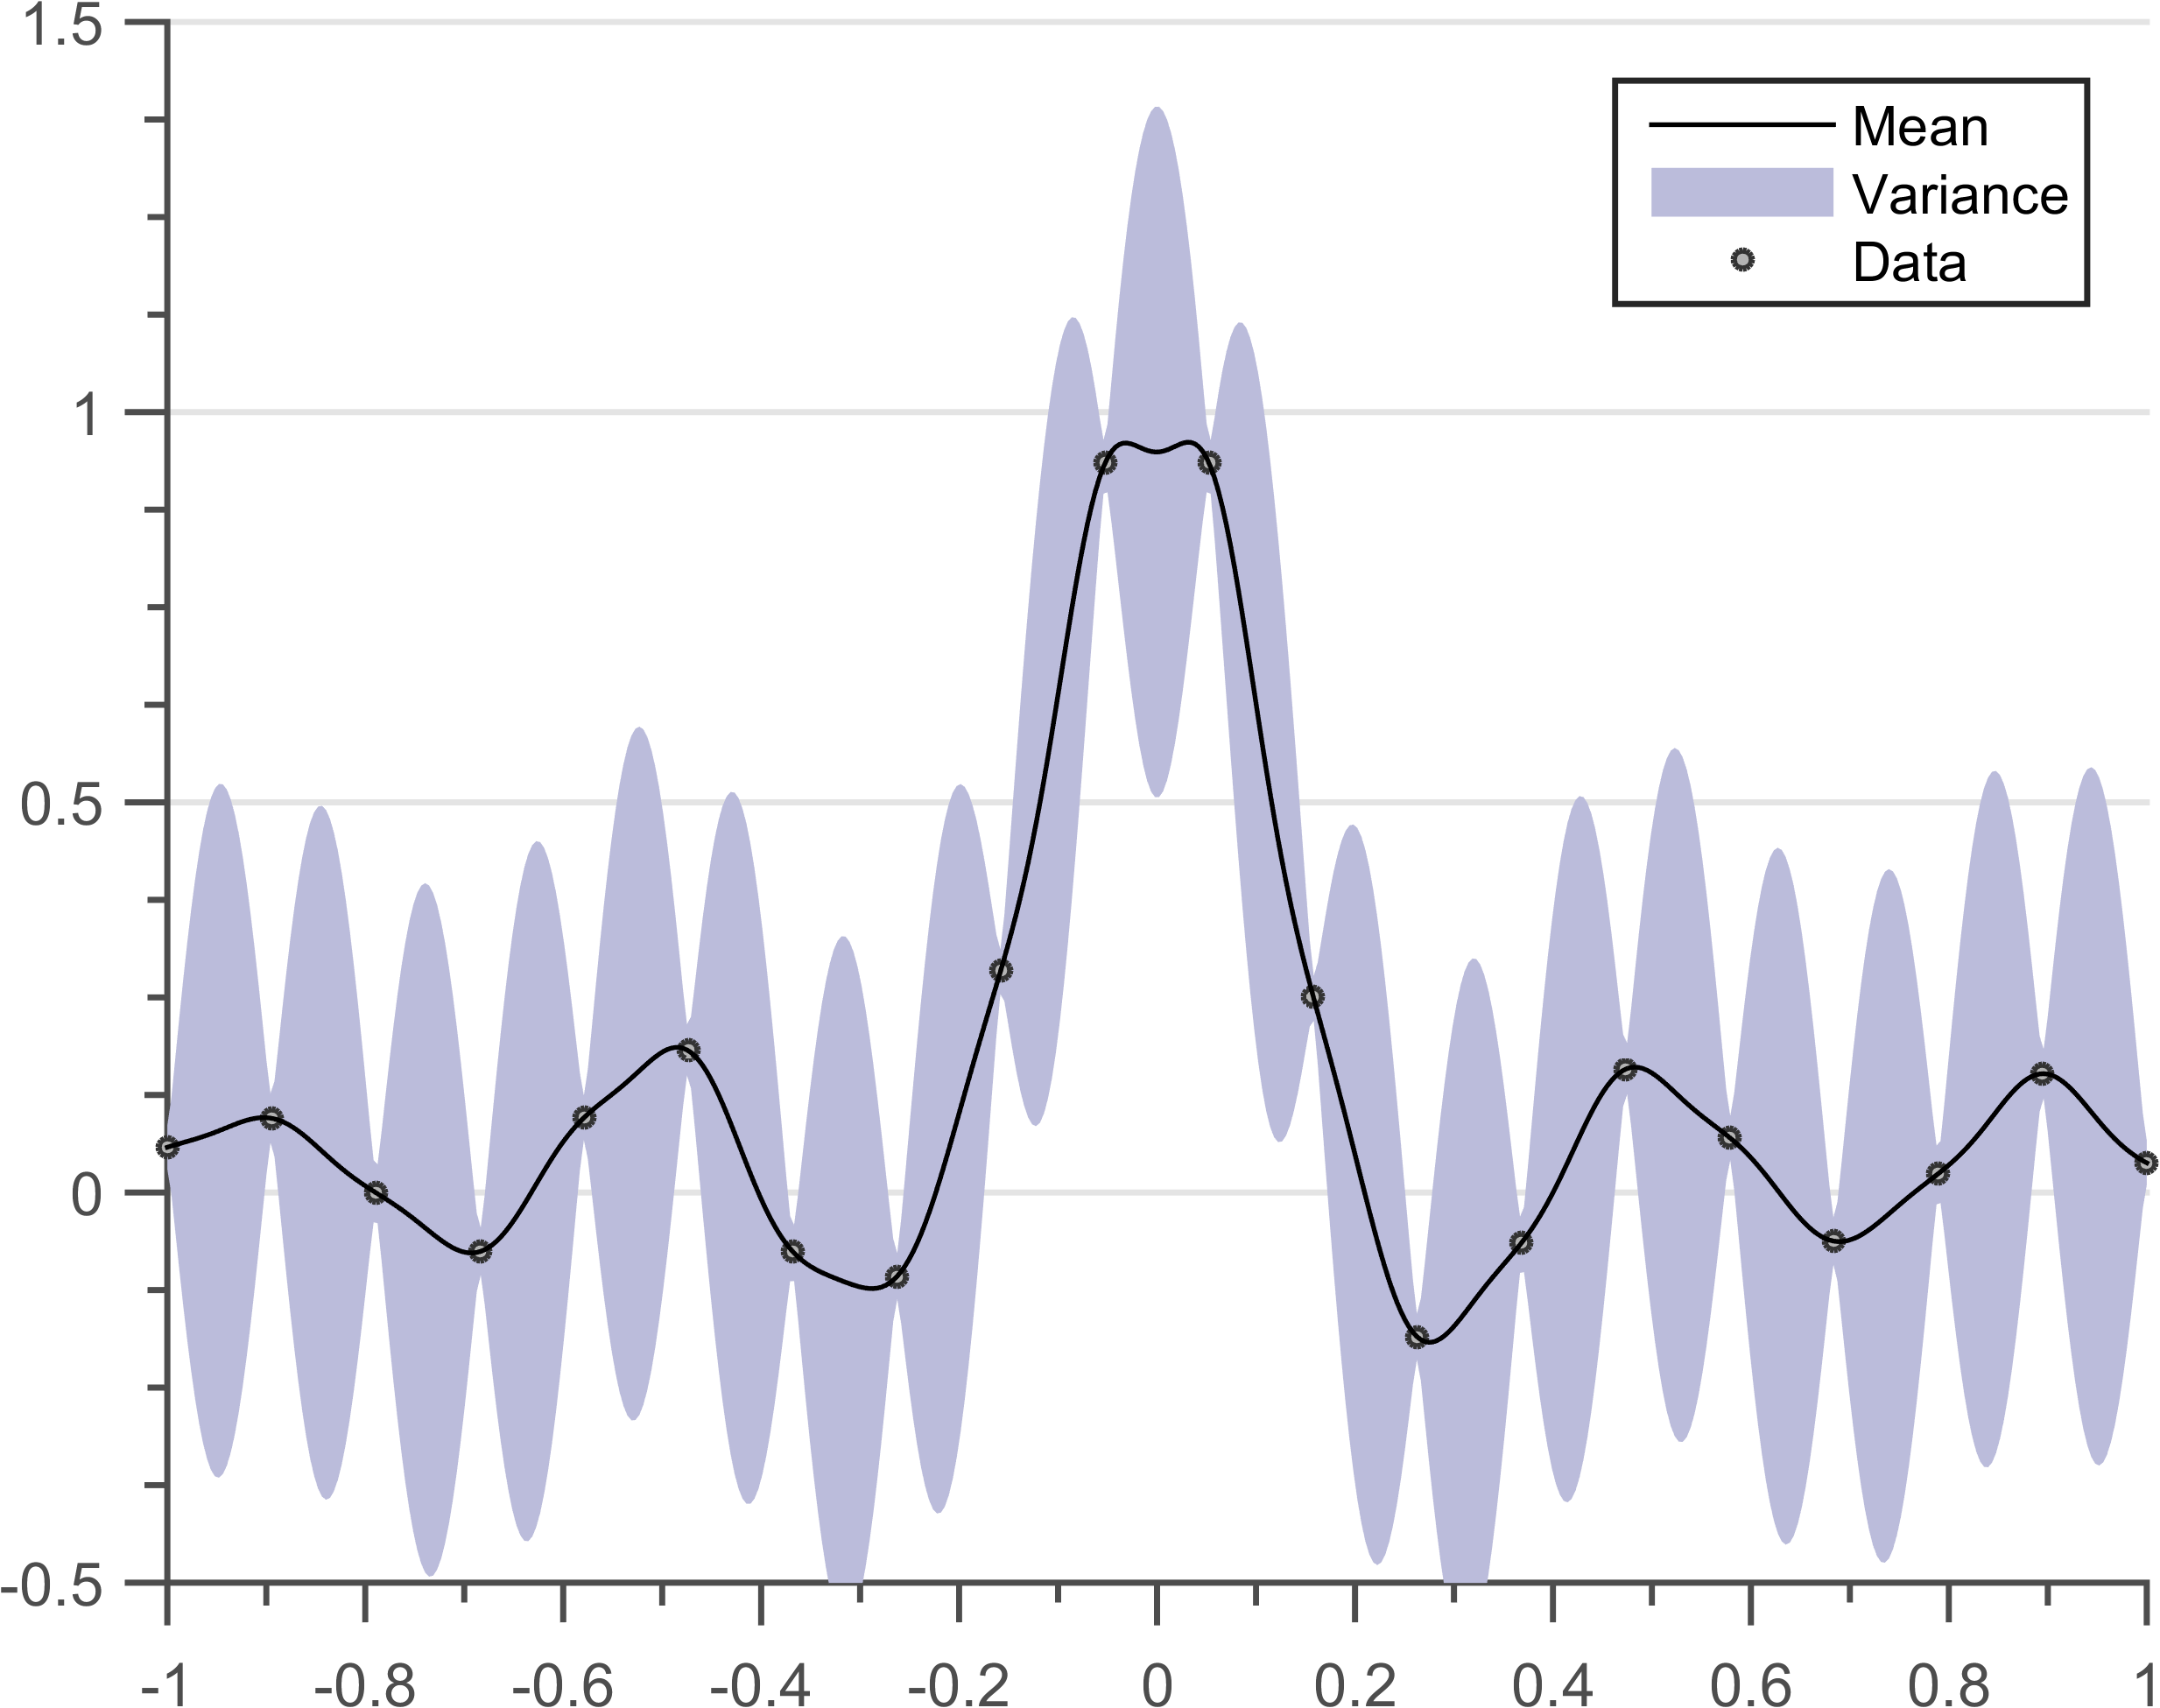
\includegraphics[width=0.45\textwidth]
        {images/part1/posteriorSE1}
        \label{subFigPosterior1}
  }\quad
\subfigure[{Posterior between SE prior with hyper-parameters $(\theta = [0.35, 0.5]; \sigma_{noise} = 0.01)$ and data. }]
%$\log (ML) = -8.2$}]
  {
        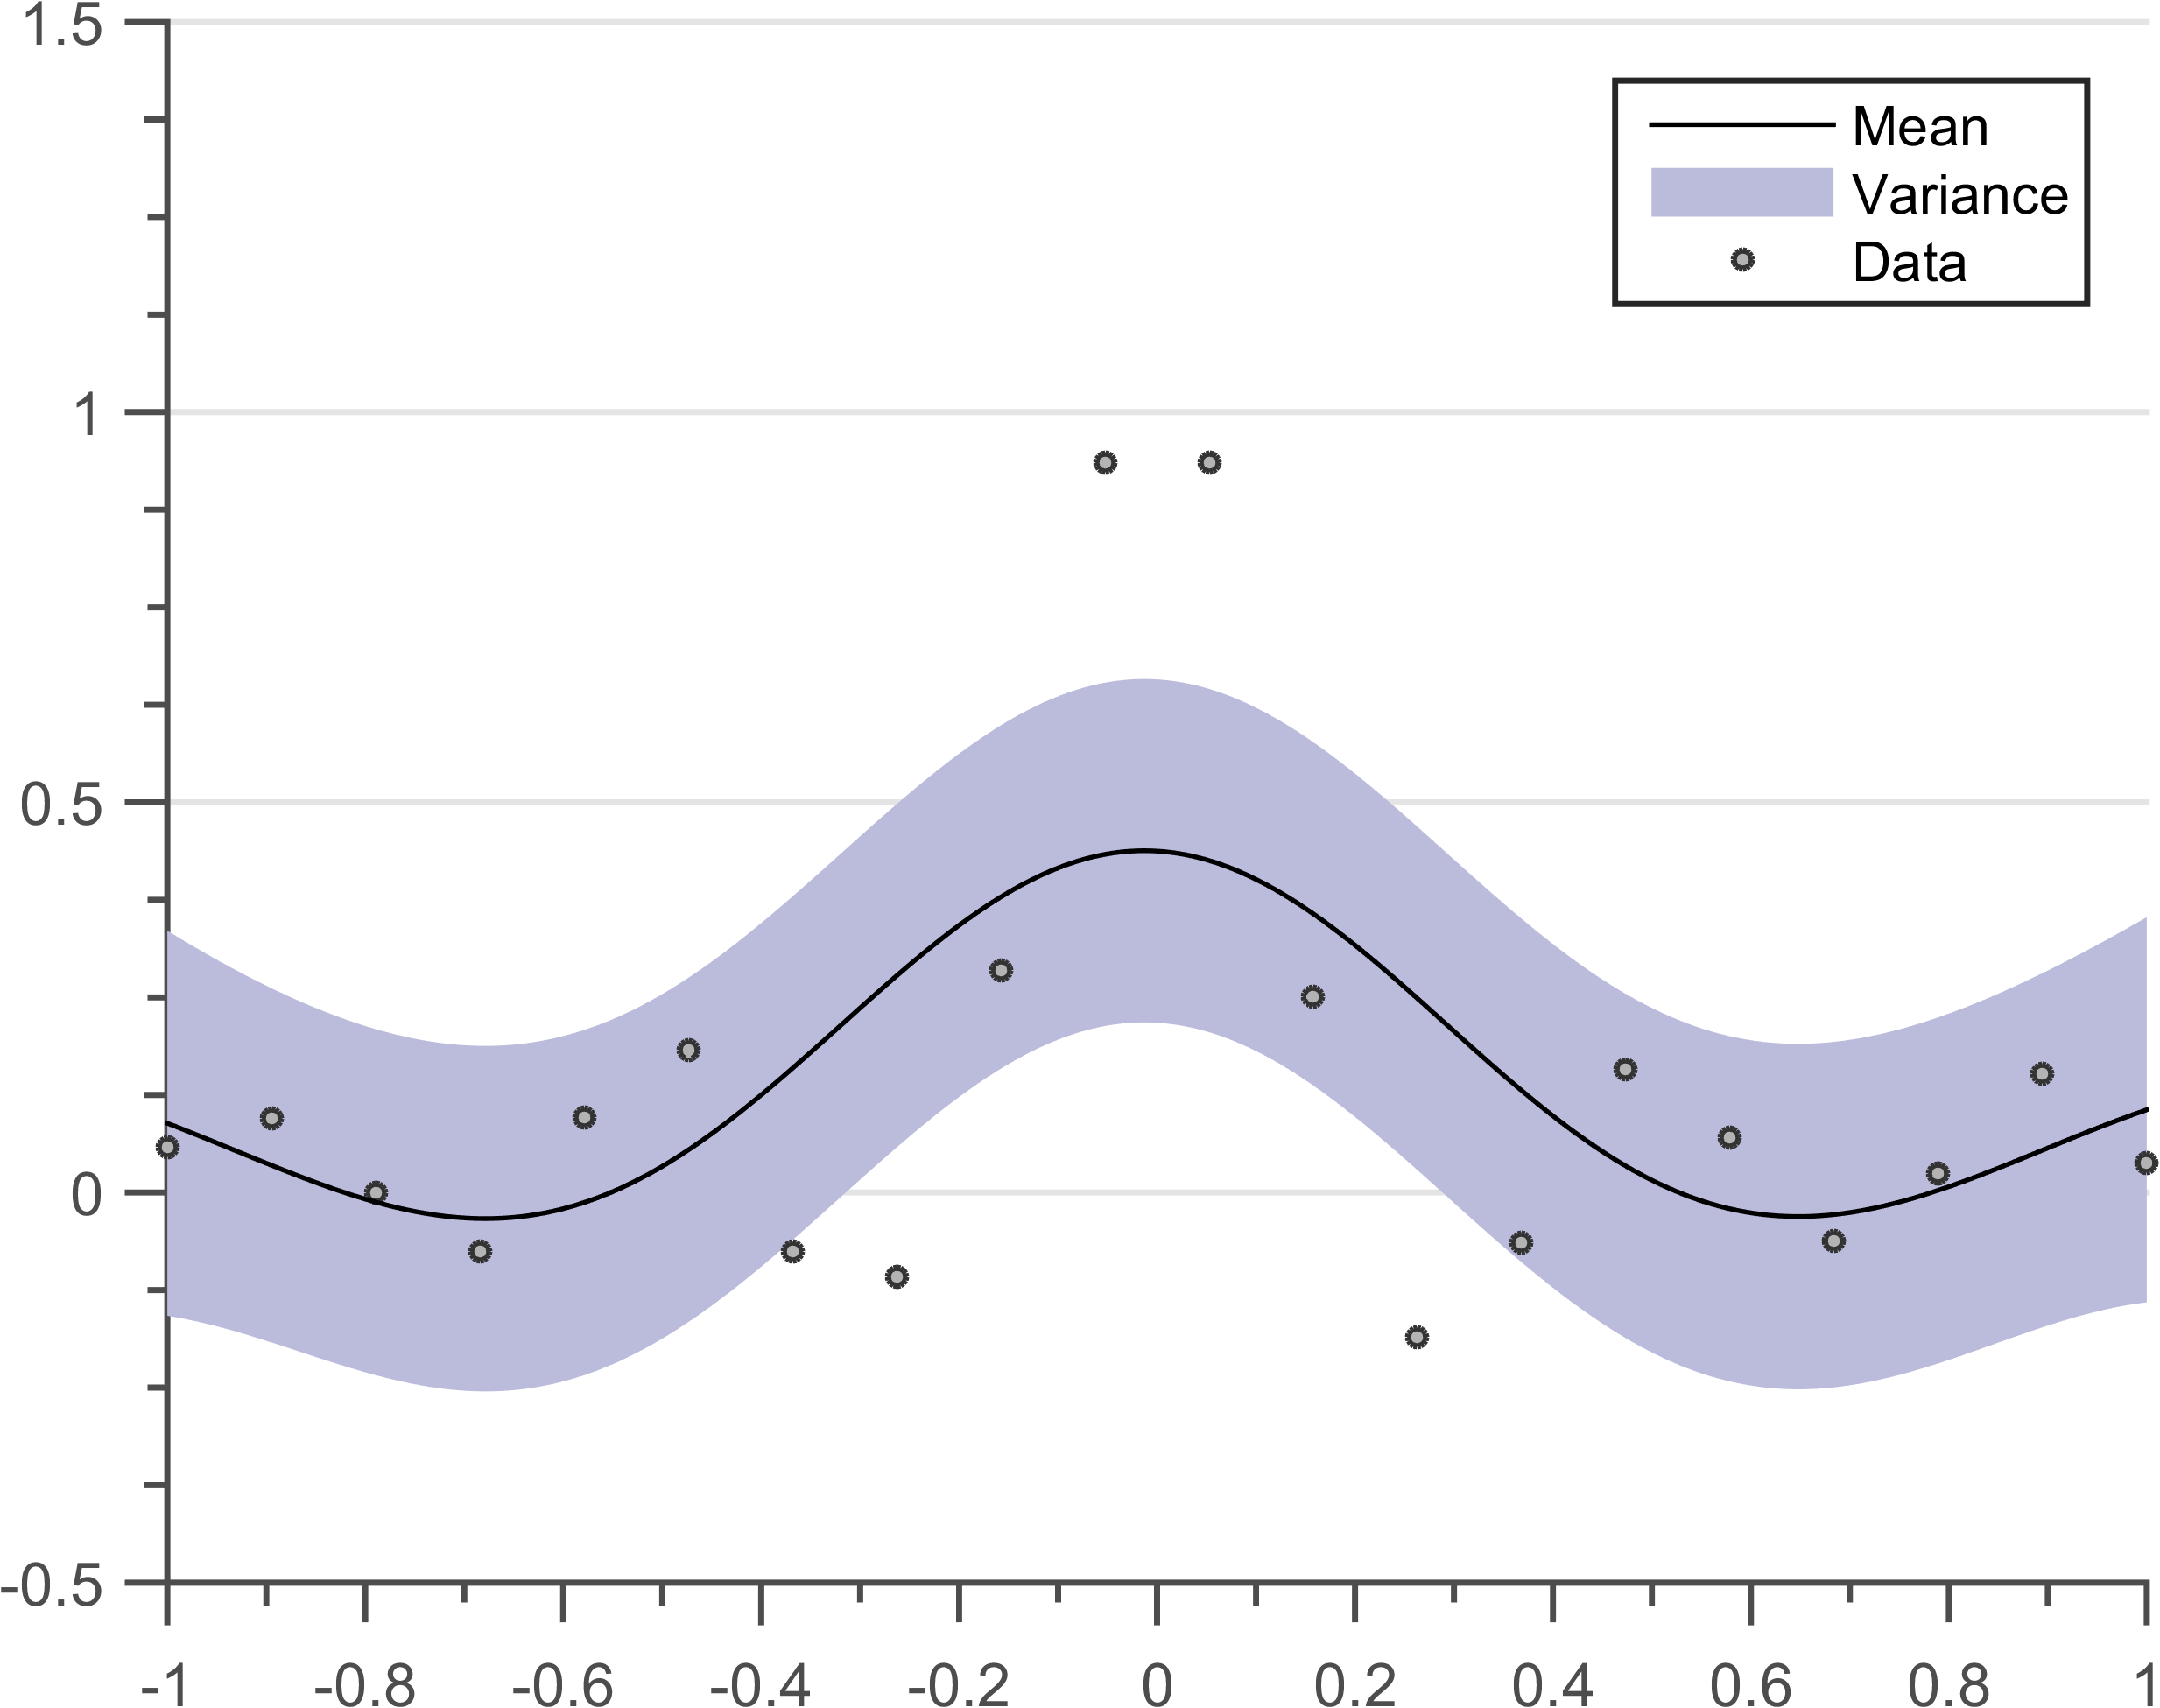
\includegraphics[width=0.45\textwidth]
        {images/part1/posteriorSE3}
        \label{subFigPosterior3}
  }\quad
       \caption{Posteriors for 2 different sets of hyper-parameters. Solid black line defines the mean function, blue region defines 95\% confidence interval (2$\sigma$) distance away from mean. }\label{figGPRMarginal}
\end{figure}

Since hyper-parameters control the family of functions in the hypothesis space and are equivalent to parameters $w$, in a pure Bayesian framework we should put a prior over our hyper-parameters $\Pr[\theta]$ and use Bayes Rule to estimate the posterior $\Pr[\theta \mid \mathcal{D}]$ over our data set. However, this approach becomes intractable and several sampling schemes have been proposed to calculate the posterior of hyper-parameters \cite{osborne2010bayesian, neal2011mcmc}.

Another method to find the optimal hyper-parameters is by performing Cross-Validation (CV). CV procedure is to split the experimental design set into two disjoint sets, one is used for training and the other one is used to monitor the performance
of the surrogate model. A particular case of CV is the Leave-One-Out (LOO) where test sets are obtained by removing one observation at-a-time. Although this can be time-consuming, there are computational short-cuts available for this scheme \cite{rasmussen2006gaussian, dubrule1983cross, le2013multi}. 

In this manuscript we neither put a prior over our hyper-parameters nor use LOO-CV for choosing hyper-parameters. We use the marginal likelihood also called evidence to find optimal hyper-parameters \cite{mackay2003information}. The probability of generating the observations $(Y)$ at the points $(X)$ from a prior (defined by $k(x_{1}, x_{2}, \theta)$) is called the marginal likelihood $\Pr[Y \mid X, \theta]$. In other words, marginal likelihood is the probability that our data set $\mathcal{D}$ was generated from a particular prior. Hence, when we maximize a marginal likelihood we are finding the best prior that could generate our data set. Using equation \ref{equationMeanZeroGPNoisydefinition} and \ref{equationJointPriorNoisy} we get:

\begin{equation}\label{equationMarginalLikelihood}
\begin{aligned}
\Pr[Y(X) \mid X, \theta, \sigma_{n}] & = \mathcal{N}(0 , K(X, X') + \sigma^{2}_{n}I)  \\
& = \frac{1}{\sqrt{(2\pi)^{N/2} K_{XX}}} exp^{-\frac{1}{2}Y^{T}K_{XX}Y}
\end{aligned}
\end{equation}

 Directly, maximizing the marginal likelihood with respect to the hyper-parameters can be inefficient. This is because the marginal likelihood does not vary significantly with the hyper-parameters. Hence to speed up the optimization process we generally maximize the log of marginal likelihood. 

  \begin{equation}\label{eqExactNLML}
\log(\Pr [Y \mid X, \theta ]) = -\frac{1}{2}Y^{T}[K_{XX}+ \sigma_{noise}^{2}I]^{-1}Y - \log\left |  K_{XX}+ \sigma_{noise}^{2}I\right | - \frac{n}{2}\log(2\pi)
  \end{equation}
  
The marginal likelihood is a trade-off between a data-fit term $(\frac{1}{2}Y^{T}K_{XX}^{-1}Y)$ and a model complexity term $(\log\left |  K_{XX}\right |)$. The optimization of ML($\theta$) provides the best compromise in terms of explaining the existing data set \{($x_{i}, y_{i}$)\} and the initial assumptions encoded in the prior. 

\textbf{define an optimization problem}

\begin{mdframed}[hidealllines=true,backgroundcolor=lightgray!20]
\lstinputlisting[caption={Optimizing the Log Marginal Likelihood}, 
                    captionpos=b, 
                    label={codeOptimizingLML}, 
                    backgroundcolor = \color{MatlabCellColour},
                    style=Matlab-editor]
                    {codes/chapter2/optimizingLogMarginalLikelihood.m}
\end{mdframed}

Figure \ref{subFigmaximizingMarginalLikelihood} shows the contours of marginal likelihood with respect to length-scale $\theta_{lengthScale}$ and noise $\sigma_{n}$ hyper-parameters. The data set is same as used in figure \ref{figGPRMarginal} and the prior is a zero mean with SE kernel. Figure \ref{subFigPosteriorOptimized} shows the posterior for same data set as used in figure \ref{figGPRMarginal} but for the hyper-parameters where marginal likelihood is maximum. The marginal likelihood could have multiple maximas in the space of hyper-parameters, hence care should be taken while initializing hyper-parameters for optimizing the log of marginal likelihood. 

  \begin{figure}[!ht]
  \centering
    \subfigure[{Marginal likelihood contours for varying noise and length-scale parameter. The amplitude hyper parameter is $(\theta_{amplitude} = [0.35])$.  Also shown on the figure are locations of hyper-parameters for figures \ref{subFigPosterior1} and \ref{subFigPosteriorOptimized}.}]
  {
        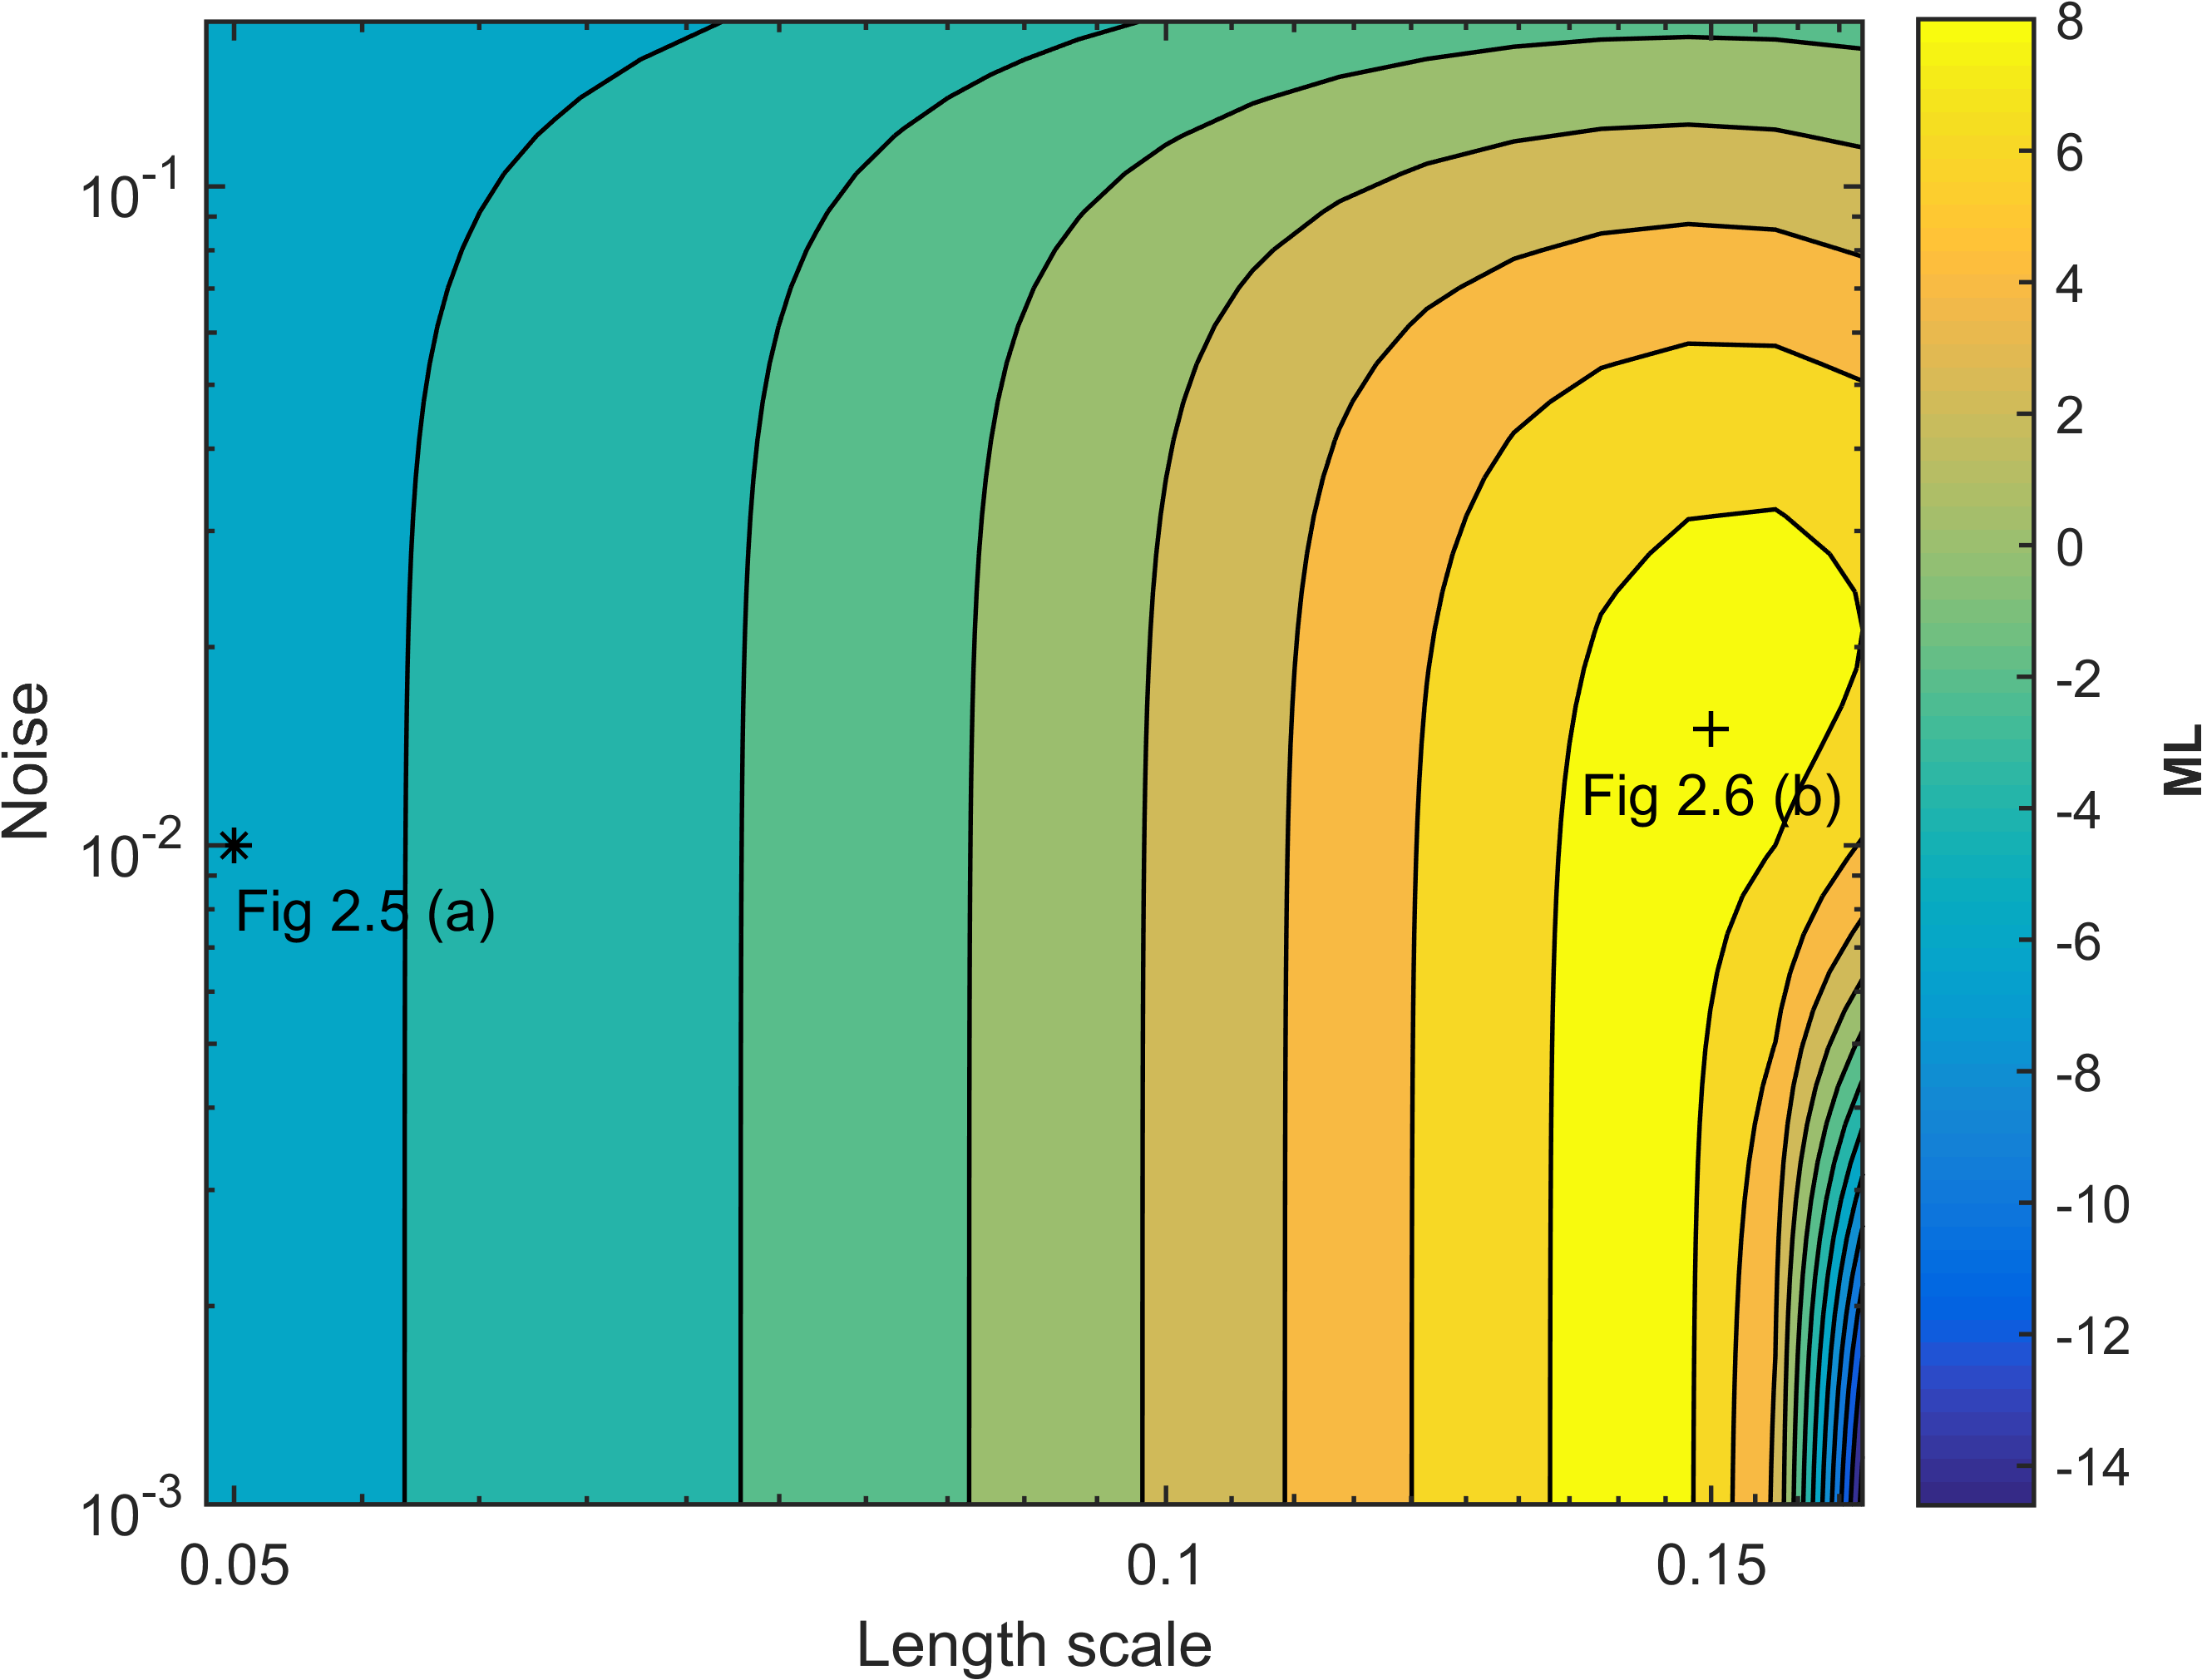
\includegraphics[width=0.45\textwidth]
        {images/part1/maximizingMarginalLikelihood}
        \label{subFigmaximizingMarginalLikelihood}
  }\quad
  \subfigure[{Posterior between SE prior with optimized hyper-parameters $(\theta = [0.35, 0.15]; \sigma_{noise} = 0.015)$ and data. $\log( ML) = 8.04$. Solid black line defines the mean function, blue region defines 95\% confidence interval (2$\sigma$) distance away from mean.}]
  {
        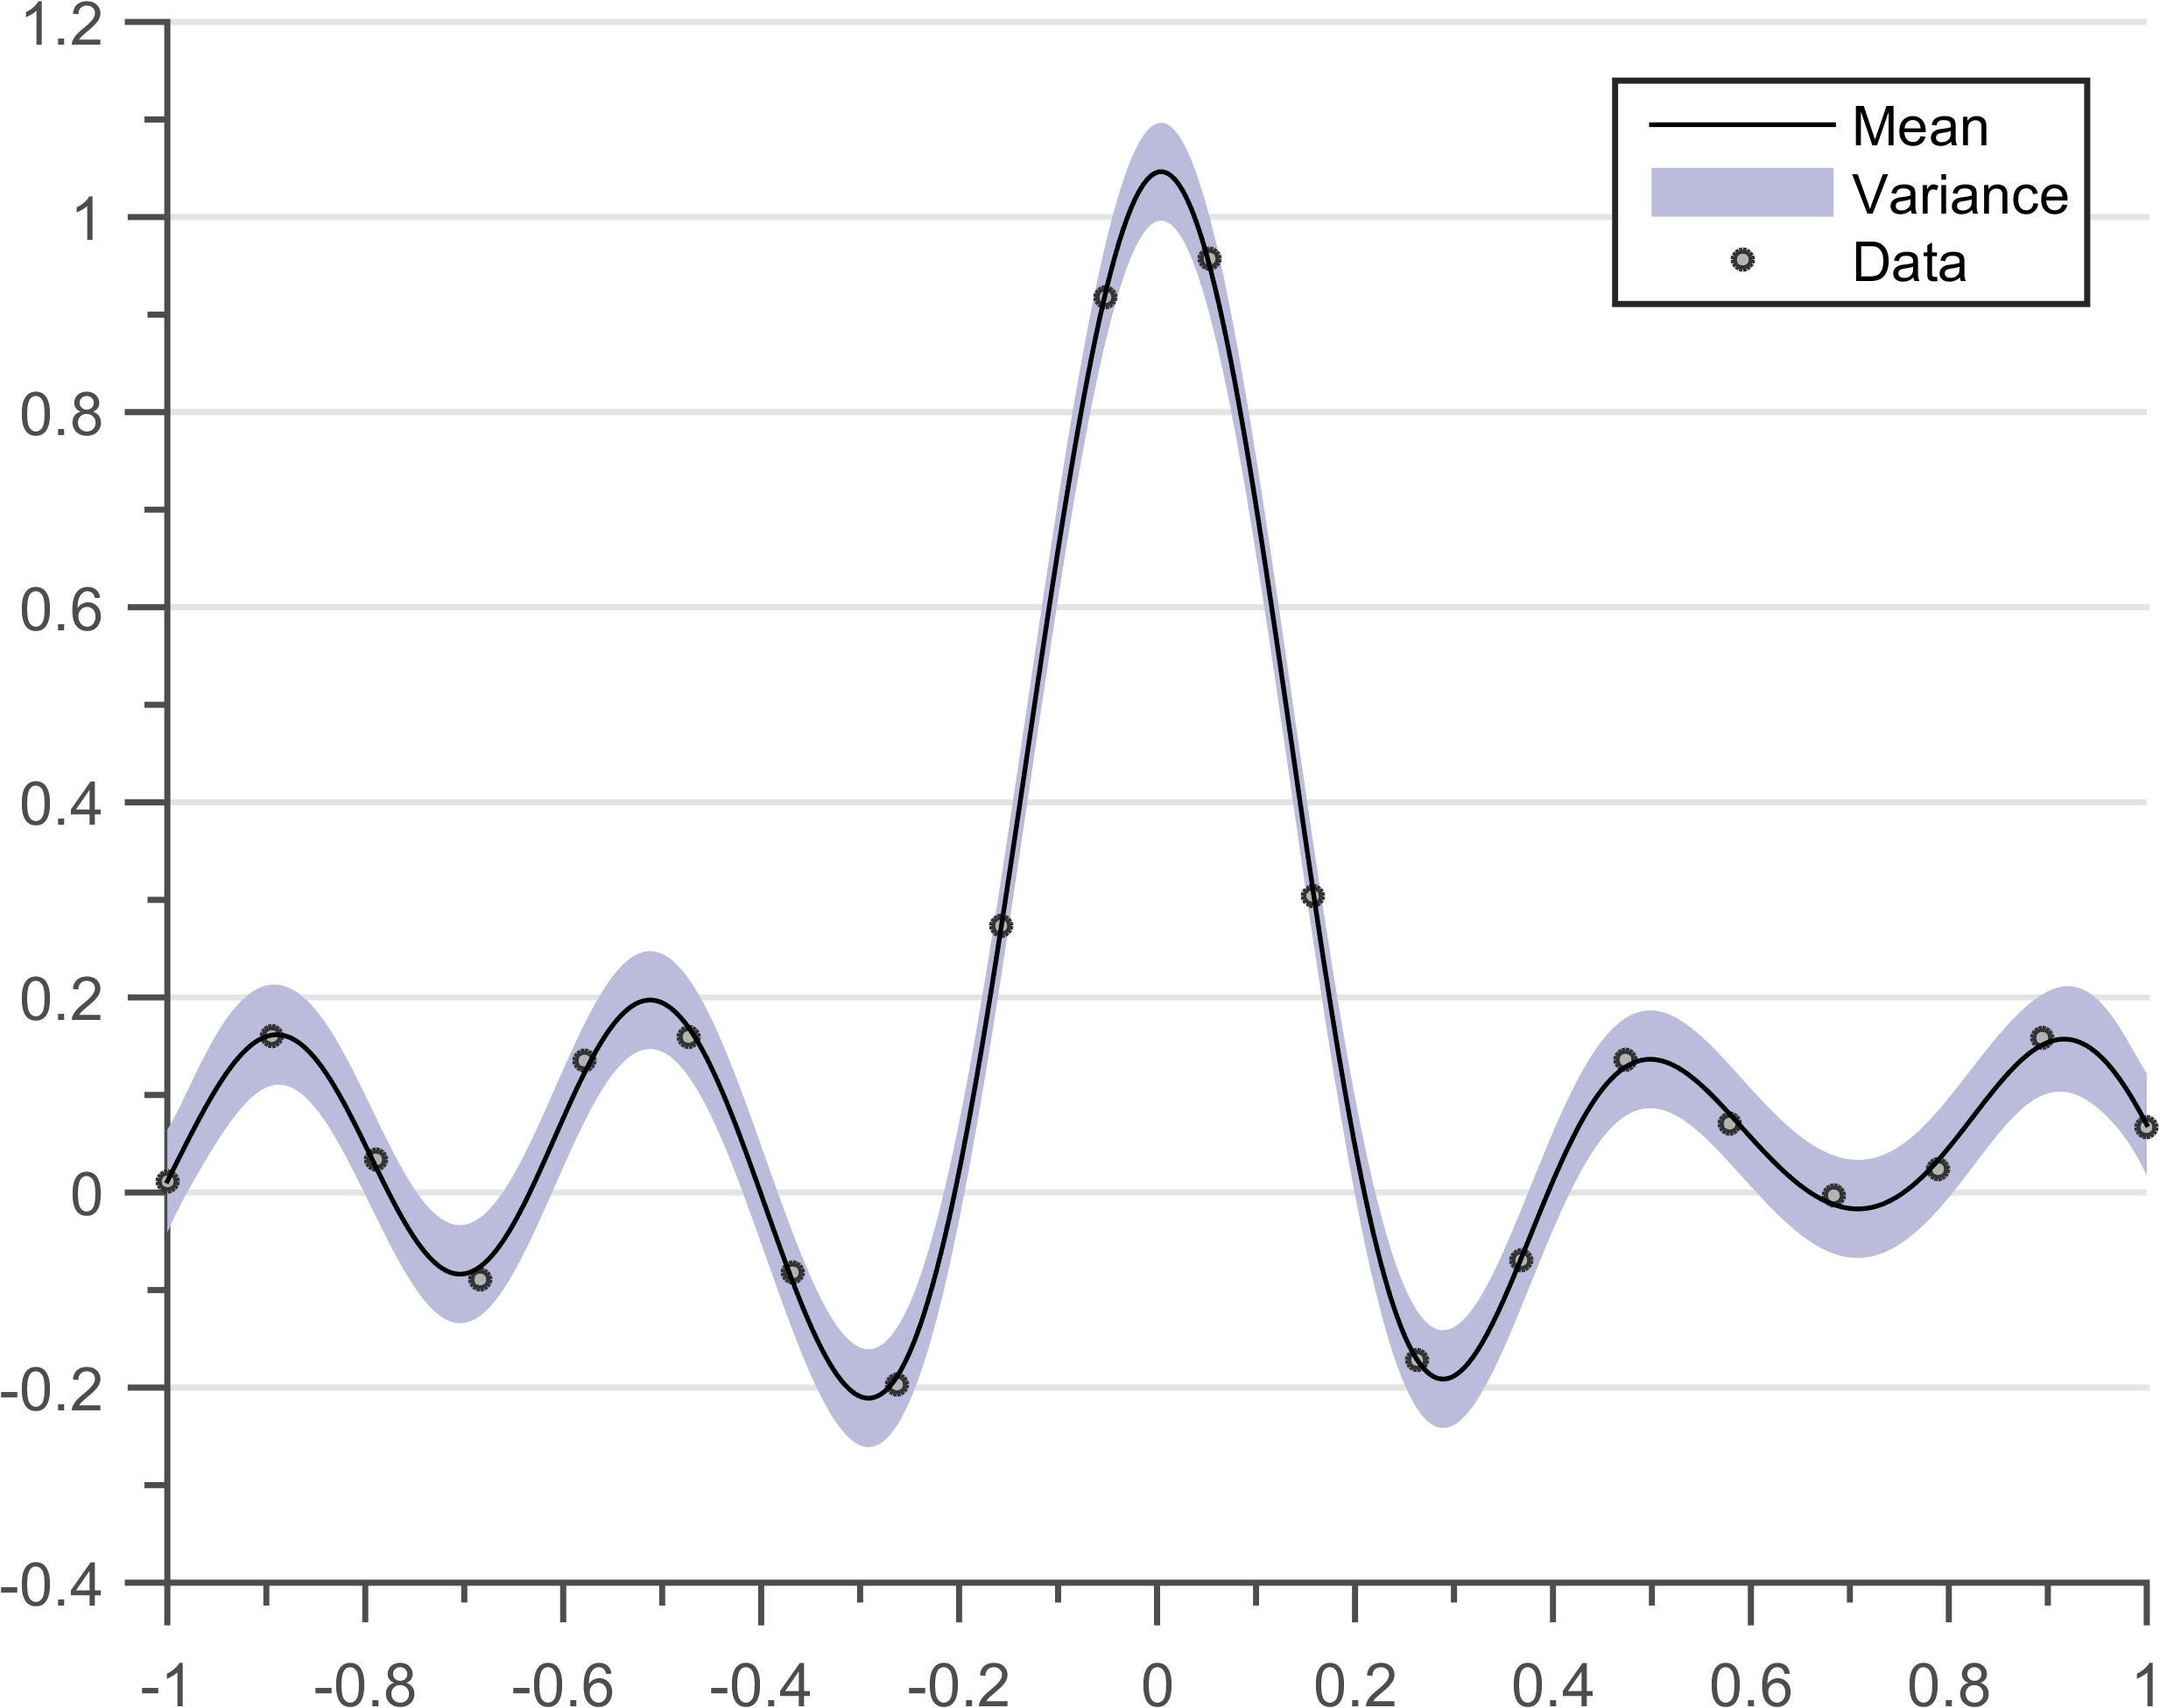
\includegraphics[width=0.45\textwidth]
        {images/part1/posteriorSE}
        \label{subFigPosteriorOptimized}
  }\quad
       \caption{Maximizing marginal likelihood}\label{figGPRMarginalOptimized}
\end{figure}

\section{Discussion}\label{secCH2Discussion}
In this chapter we provide a brief introduction on how to perform Regression with GPs. GPs are the ideal candidate for regression due to their marginalization property, which makes them computationally tractable. Even if GPs define an infinite dimensional random vector, inference on a few points does not require the presence of infinitely other points. This makes drawing functions, calculating posterior distribution and automating selection of hyper-parameters computationally feasible. Thereby making GPs an ideal candidate for defining a Prior distribution in a Bayesian Regression framework. 

The section \ref{secPrior} details the key constituents of a GPs. A GP can be completely parametrized by its mean and covariance function. While, the trend of a GP is defined by its mean function, the structure of its constituent functions is defined by the covariance function. Normally the mean of a GP can be assumed to be zero, since an extra term in the covariance function can represent the mean function. Hence the problem of learning in a GP is exactly the problem of finding suitable properties of the covariance function (subsection \ref{subSecCH2Covariance}). Once a function form of covariance is chosen we can calculate the Gram matrix at desired points and use it to draw random functions from our prior (subsection \ref{subSecSamplingFunctionsGPPrior}). 

The next section \ref{secPosterior} describes how to calculate the posterior distribution. The posterior is the conditional distribution $(\Pr[f(x_{*}) \mid Y, X, \theta])$ for an assumed Prior distribution $(\Pr[f] = GP(0, k(x_{1}, x_{2}, \theta))$ and a set of observed data points $(\mathcal{D} = {X, Y})$. Again, due to the Gaussian assumption the conditional probabilities are all computationally tractable and can be calculated using a few matrix operations, side-stepping the computational burden of performing iterative sampling. Calculating the posterior is easy both in the absence (subsection \ref{subSecPosteriorNoiseFree})and presence (subsection \ref{subSecPosteriorNoisy}) of noise in observations. 

Given a functional form of the covariance, section \ref{secHyperParameter} shows the importance of choosing the correct hyper-parameters. In a pure Bayesian framework the posterior distribution of the hyper-parameters should be calculated ($\Pr[\theta \mid \mathcal{D}]$), but this is computationally intractable needing several iterations for calculation of integrals. A common practice in the community is maximizing the marginal likelihood to automatically choose the hyper-parameters. Marginal likelihood is the probability of a prior distribution $\Pr[f] = GP(0, k(x_{1}, x_{2}, \theta)$ generating the observations $\mathcal{D}$. Hence maximizing the marginal likelihood gives the optimal set of hyper-parameters for a functional form of covariance function (figure \ref{figGPRMarginalOptimized}). 

Calculating the precision matrix $[K_{XX}+ \sigma_{noise}^{2}I]^{-1}$ is an important task in calculating the marginal likelihood (equation \ref{}), posterior mean (equation \ref{}) and covariance (equation \ref{}). Unfortunately, this task has a computational complexity of $\mathcal{O}\left ( N^{3} \right )$ and memory footprint of $\mathcal{O}\left ( N^{2} \right )$. Putting an upper limit of $N \sim 10^4$ on the number of data points, a standard laptop cannot store such a big matrix for inversion \footnote{The computer runs out of memory before we run out of patience :p}. The next chapter describes few methods of performing approximating inference which scales GPs to $N \sim 10^6$ or more data points. 
\chapter{Scaling up Gaussian Process Regression}
\label{chapScalingGPR}

The GP regression approach as mentioned in earlier chapter is intractable for large data sets. For a data set of size $N$ the covariance matrix $K_{XX}$ is of size $N \times N$,  where $\mathcal{O}\left ( N^{3} \right )$ time is needed for calculating the precision matrix and $\mathcal{O}\left ( N^{2} \right )$ memory for storage. Since, inverting the covariance matrix takes considerable amount of time and memory, almost all techniques to scale up GP regression try to approximate the inversion of Gram matrix $K_{XX}$. 

Let us take the example of an SE kernel, for a large value of length-scale the Gram matrix ($K_{XX}$) is spread out and has a rank lower than  $N$ (figure \ref{subFigSEPrior_2}). Due to this low-rank characteristic the Gram matrix can be approximated as a lower rank form reducing the cost of inverting the Gram matrix. In the GP literature sparse approximations (section \ref{secSparseApprox}) use a set of inducing points to compress the information of the several observations through the low-rank approximation. 

For the same SE kernel if the length-scale tends to a low value the Gram matrix is not of low-rank but tends to a diagonal matrix (figure \ref{subFigSEPrior_1}). In the GP literature the mixture of experts (section \ref{secDgp}) methodology exploits the block diagonal nature of the Gram matrix by distributing data points into a subset of experts, assuming independence across experts and distributing the calculations into several batches. The first regime suggests global (numerical) low-rank approximations while the second regime suggests local block-diagonal approximations \cite{march2015askit, chenhan2016inv}. 

The remaining chapter unfolds as follows, section \ref{secSparseApprox} describes the Sparse Approximations detailing several methods of choosing inducing points and then performing experiments on a toy dataset. Section \ref{secDgp} describes the Distributed GP methodology detailing several methods for merging of experts and then performing experiments on the same toy-dataset. 

\section{Sparse Approximations}\label{secSparseApprox}
Sparse methods use a small subset of input points as support or inducing points to approximate the Gram matrix. Suppose we use $M$ inducing points $X^{m} = \{x^{m}_{1}; x^{m}_{2}; \ldots; x^{m}_{M}\}$, such that $M < N$. The points $X^{m}$ can be a subset of training inputs in the input space. 


\subsection{Nystr\"{o}m Approximation}\label{subSecNystrom} 

Using Nystr\"{o}m approximation the Gram matrix can be approximated as equation \ref{eqnSparseNystormGram} \cite{quinonero2005unifying, seeger2003fast}, for more detail refer to appendix \textbf{refer to link in the appendix}. 

\begin{equation}\label{eqnSparseNystormGram}
K_{nystorm}(X, X) = K(X, X^{m})K(X^{m}, X^{m})^{-1}K(X^{m}, X)
\end{equation}

Here, $K(X^{m}, X^{m})$ is a $M \times M$ Gram matrix evaluated at inducing points $X^{m}$, $K(X, X^{m})$ is an $N \times M$ Gram matrix between training points and inducing points. The inversion of approximate matrix takes $\mathcal{O}\left ( NM^{2} \right )$ time to compute. Figure \ref{subFigNystormSEmatrix} is an approximate Gram matrix using Nystr\"{o}m approximation of the matrix in figure \ref{subFigcovSEmatrix_1} at the input points $X^{*} = \{[0:0.02:1]\}$. The inducing points $X^{m}$ were chosen randomly from the set of input points and their location is denoted by white lines. We can observe that if the gap between inducing points increases then accuracy of Gram matrix degrades (eg. at $x \sim 0.5$). Figure \ref{subFignystormSEmatrixUniform} is again an approximated Gram matrix using Nystr\"{o}m approximation of the matrix in figure \ref{subFigcovSEmatrix_1}. This time the equally spaced inducing points are chosen in the range of $X^{*}$. Notice the significant improvement in the Gram matrix upon different set of inducing inputs.

\begin{figure}[!ht]
  \centering
    \subfigure[{Approximated Gram matrix using Nystr\"{o}m approximation for a Standard Exponential (SE) Kernel with $(\theta = [1, 0.2])$ (figure \ref{subFigcovSEmatrix_1}) at the input points $X^{*} = \{[0:0.02:1]\}$. The inducing points were chosen randomly, the white lines denote the location of inducing points. }]
  {
        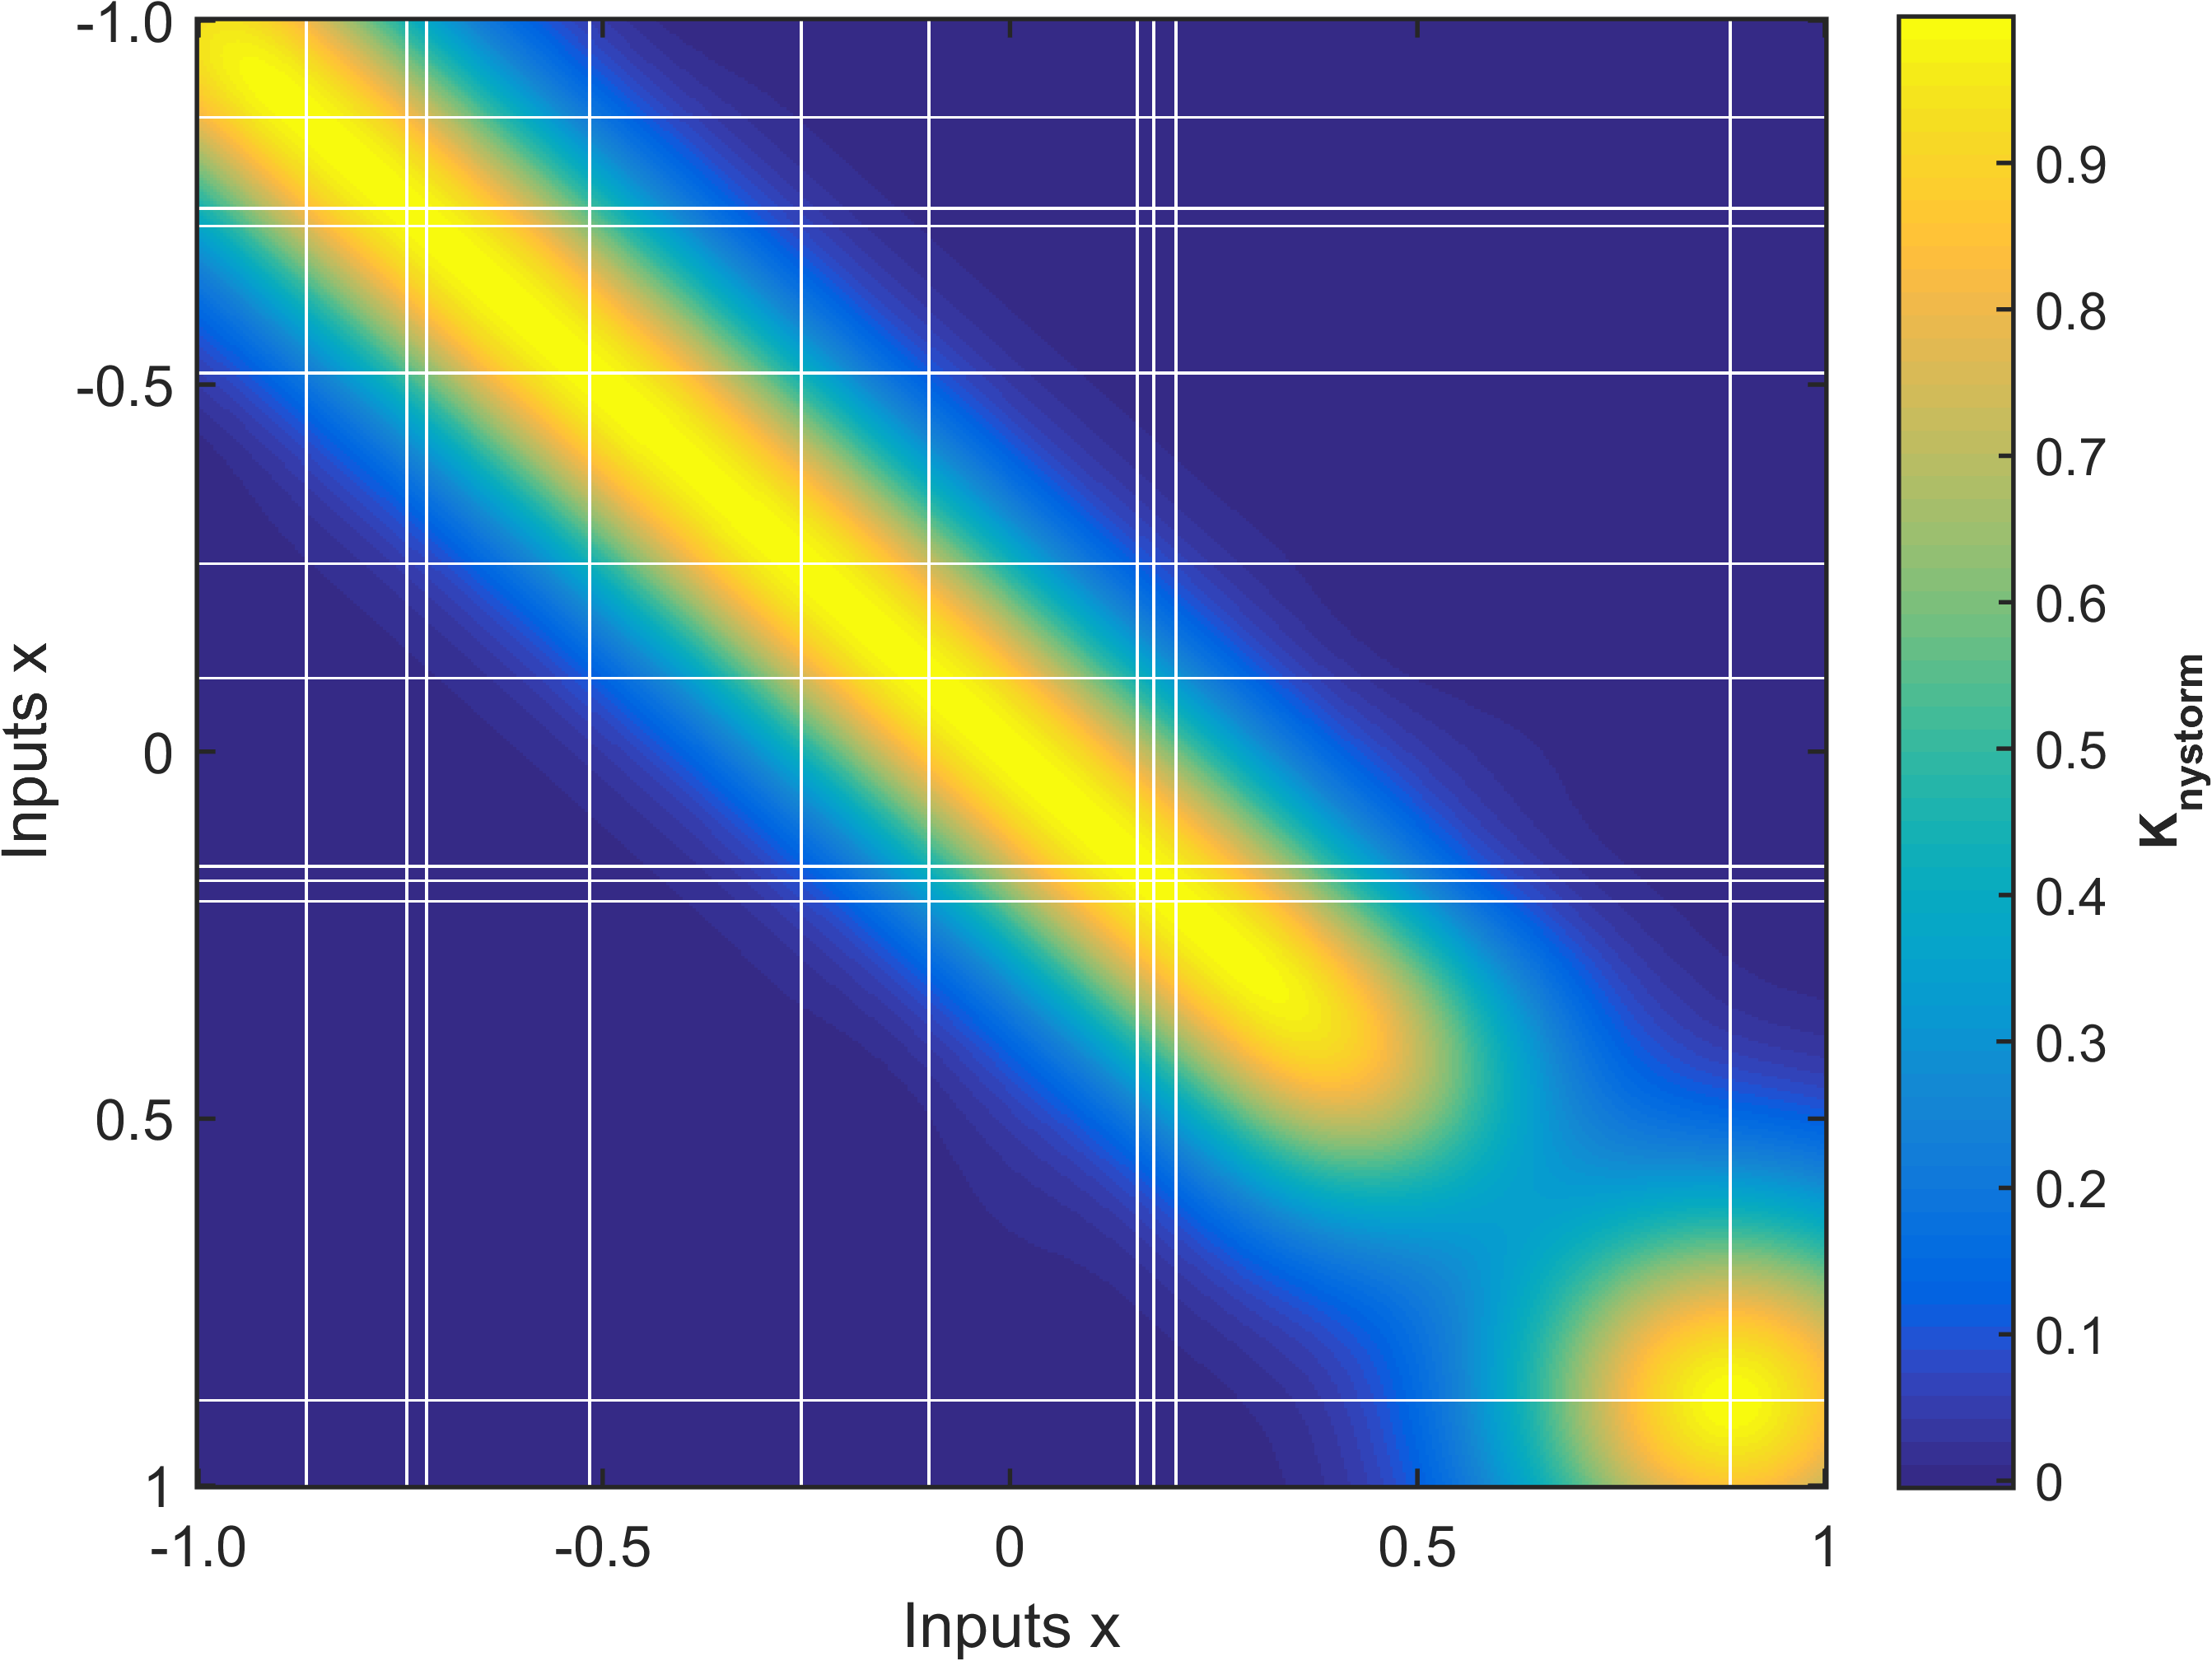
\includegraphics[width=0.45\textwidth]
        {images/part1/nystormSEmatrix}
        \label{subFigNystormSEmatrix}
  }\quad
\subfigure[{Approximated Gram matrix using Nystr\"{o}m approximation for a Standard Exponential (SE) Kernel with $(\theta = [1, 0.2])$ (figure \ref{subFigcovSEmatrix_1}) at the input points $X^{*} = \{[0:0.02:1]\}$. The white lines denote the location of inducing points, the inducing points are uniformly distributed. Notice the significant improvement in Gram matrix due to different inducing inputs}]
  {
        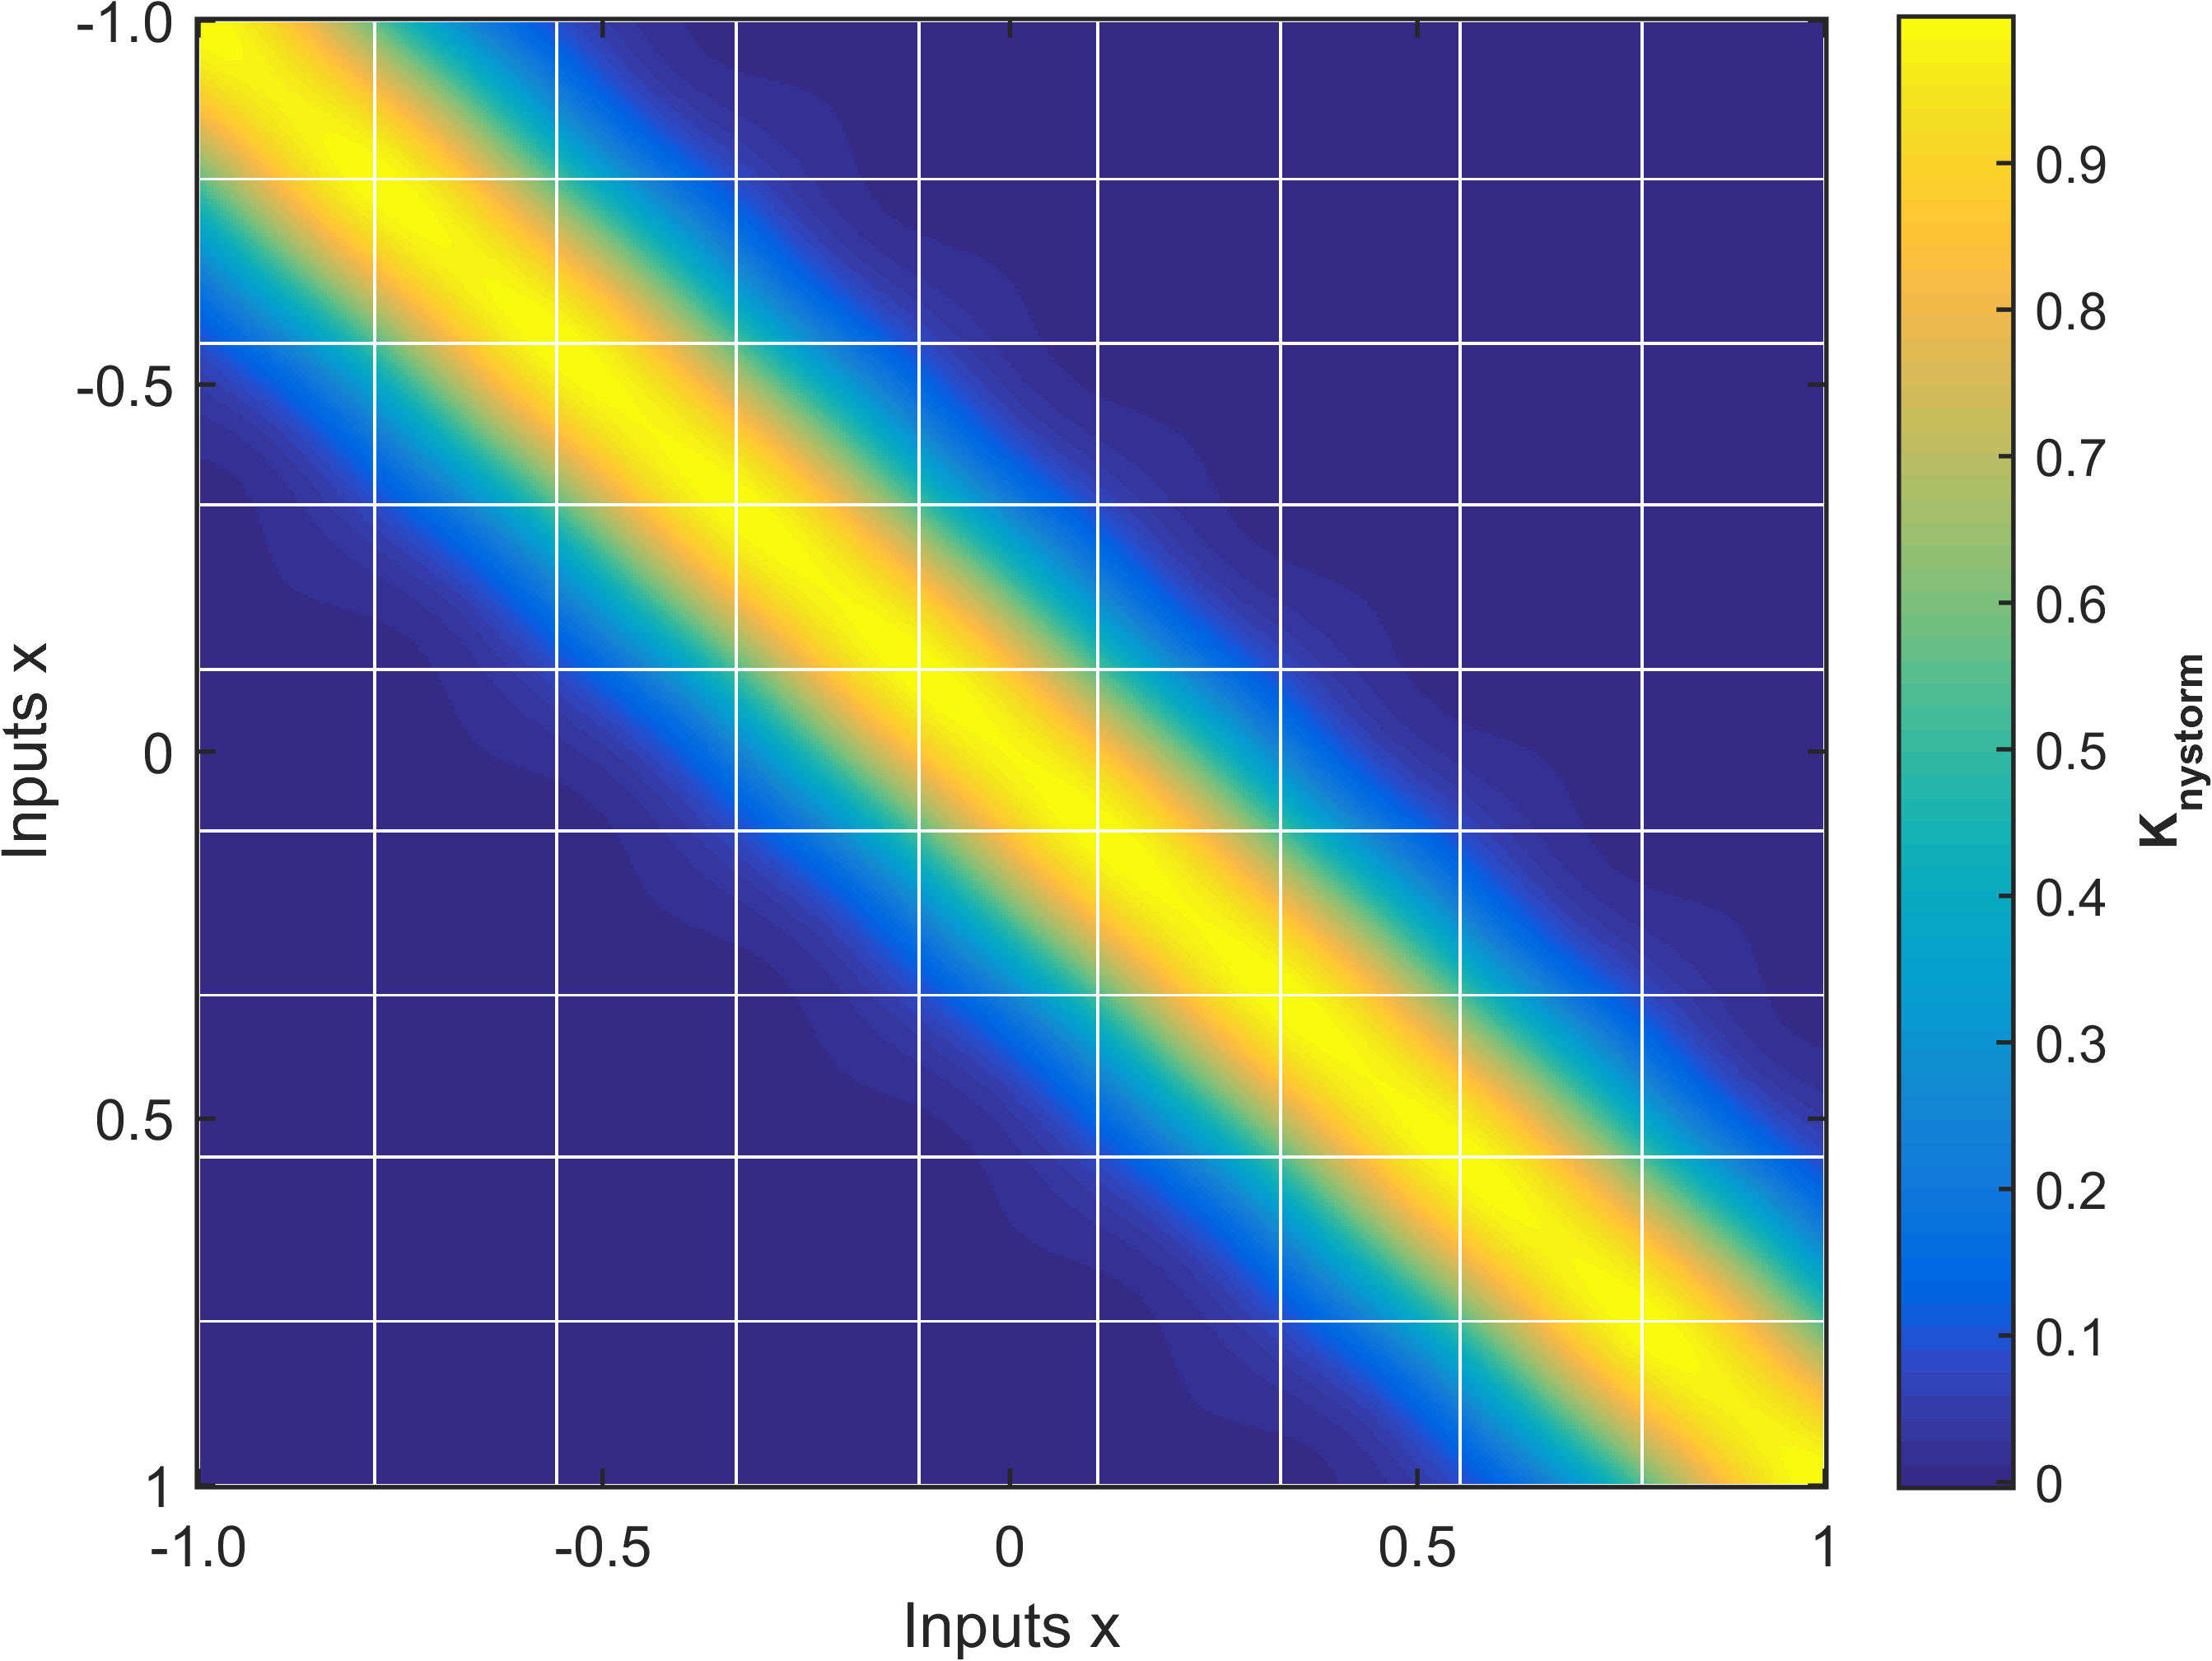
\includegraphics[width=0.45\textwidth]
        {images/part1/nystormSEmatrixUniform}
        \label{subFignystormSEmatrixUniform}
  }\quad
  
       \caption{Approximate Gram matrix for a Standard Exponential kernel using Nystr\"{o}m approximation.}\label{figGPNystormGramMatrix}
\end{figure}

Later, \cite{Snelson06sparsegaussian} proposed the FITC approach which corrects the diagonal terms of the Gram matrix and improves the prediction capabilities (equation \ref{eqnSparseNystormGram}).

\begin{equation}\label{eqnSparseFITCGram}
K_{FITC}(X, X) = diag[K(X, X) - K_{nystorm}(X, X)] + K_{nystorm}(X, X)
\end{equation}

Note, calculating $diag(K(X, X))$ is an $\mathcal{O}\left ( N \right )$ operation and thus does not significantly impact the time taken. 

\textbf{add comment about algorithm}

\begin{mdframed}[hidealllines=true,backgroundcolor=lightgray!20]
\lstinputlisting[caption={Gram Matrix using Nystr\"{o}m Approximation}, 
                    captionpos=b, 
                    label={codeGramNystrom}, 
                    backgroundcolor = \color{MatlabCellColour},
                    style=Matlab-editor]
                    {codes/chapter3/evaluateNystromGramMatrix.m}
\end{mdframed}


The posterior distribution for the approximate prior can be derived similarly as given in appendix \textbf{add appendix ref} and is a Gaussian. The predictive mean and predictive variance are written as equation \ref{eqNoisyNystormPredictiveMean} and equation \ref{eqNoisyNystormPredictiveCovariance}. Here, $K_{approximate}(X, X')$ can be the approximated Gram matrix either from the Nystr\"{o}m approximation (equation \ref{eqnSparseNystormGram}) or the FITC approximation (equation \ref{eqnSparseFITCGram}). 
\begin{equation}\label{eqNoisyNystormPredictiveMean}
  \mathbf{E}[f_{approximate}(x_{*})] = K_{Xx_{*}}^{T}( K_{approximate}(X, X') + \sigma^{2}_{n}I)^{-1}Y
  \end{equation}
\begin{equation}\label{eqNoisyNystormPredictiveCovariance}
	Cov[f_{approximate}(x_{*})] = K_{x_{*}x_{*}} - K_{Xx_{*}}^{T}( K_{approximate}(X, X') + \sigma^{2}_{n}I )^{-1} K_{Xx_{*}}
  \end{equation}


By approximating the $K(X, X)$ using the inducing points we have effectively changed the GP prior. This means that $X^{m}$ have also become the hyper-parameters of our GP prior. Hence, we should fine-tune locations of $X^{m}$ and the hyper-parameters $\theta$ to obtain a good prediction of our data. The marginal likelihood for the approximate prior (equation \ref{equationApproximateML}) be written similarly as equation \ref{equationMarginalLikelihood}.

\begin{equation}\label{equationApproximateML}
    \Pr[Y(X) \mid X, X^{m}, \theta, \sigma_{n}] = \mathcal{N}(0 , K_{approximate}(X, X') + \sigma^{2}_{n}I)
\end{equation}


The maximization of the marginal likelihood in equation \ref{equationApproximateML} with respect to ($X^{m}$; $\theta$), is prone to over-fitting especially when the number of inducing inputs is large. This means that if we keep on increasing the number of inducing points a time will come when we will tend to decrease the accuracy of our predictions on the test data set. The variational approximation (detailed next) approach overcomes this issue of over-fitting by adding a regularization term penalizing over-fitting.

\subsection{Variational Approximation}\label{subSecVariationalApprox} 
The variational approximation does not attempt to approximate the Gram matrix. Instead, it assumes a probability distribution $q(f)$ of the true posterior distribution $p(f \mid y)$ and minimizes the distance between the two \cite{Titsias09variationallearning}. 

The $q(f)$ is written in terms of inducing points ($X^{m}$) and the KL divergence $KL(q||p)$\footnote{KL divergence is a measure of distance between two probability distributions} is minimized between the variational distribution $q$ and true distribution $p$. When we minimize the KL divergence we are making the assumed distribution closer to true distribution and hence improving the values of ($X^{m}$) and $\theta $. This minimization of KL divergence is equivalently expressed as the maximization of the equation \ref{equationLowerBoundVarNLML}

\begin{equation}\label{equationLowerBoundVarNLML}
F_{V} = log(\mathcal{N}[0, \sigma_{n}^{2}I + K_{nystorm}(X, X)]) - \frac{1}{2\sigma_{n}^{2}}Tr(K_{XX} - K_{nystorm}(X, X))
\end{equation}

Notice, the similarity between equation \ref{equationLowerBoundVarNLML} and \ref{eqnSparseNystormGram}. The novelty of the above objective function is that it contains a regularization term: $- \frac{1}{2\sigma ^{2}}Tr(K_{XX} - K_{nystorm}(X, X))$. Thus, $F_{V}$ attempts to maximize the marginal likelihood as derived for Nystr\"{o}m approximation and simultaneously minimizes the trace. When the regularization term tends to zero $K_{XX} - K_{nystorm}(X, X)$, which means that the inducing variables can exactly reproduce the full GP prediction. 

The posterior distribution for variational inference approximation is same as the one derived for Nystr\"{o}m approximation. The difference between Nystr\"{o}m approximation and variational approximation is the improvement in the evaluation parameter while optimizing $X^{m}$ and $\theta$. Due to the additional trace term variational inference reduces over-fitting.

\subsection{Experiments}\label{subsecNystromExperiments}
We here conduct experiments on a toy-data set to observe the accuracy of Nystr\"{o}m approximation for varying number and location of inducing points. The basic toolbox used for this paper is GPML provided with \cite{rasmussen2006gaussian} on MATLAB 2014b. All experiments were performed on an Intel quad-core processor with 4Gb RAM. 

10-fold Cross Validation (CV) will be used to assess the performance of the prediction. CV is a technique where the dataset is partitioned as the test set and training set. A model is learned using the training set and Root Mean Square Error (RMSE) is calculated between the prediction and test set as a measure of accuracy. In the 10-fold version of CV, the dataset will be randomly partitioned into 10 subsets containing an equal number of points. Of the 10 subsets, a single subset is retained as the test dataset, and the remaining 9 (10 - 1) subsets are used as training data. The cross-validation process is then repeated 10 times (the folds), with each of the k subsets used exactly once as the validation data.

The toy data set ($\mathcal{D}_{3}$) was generated at 1000 input points $X = \{[-1:0.002:1]\}$ by sampling a random function from a GP\footnote{$(\Pr[Y \mid X, \theta, \sigma_{n}] = GP(0, K_{SE}(X, X', \theta = [1, 0.1]) + (0.3)^{2}I)$} with zero mean, SE covariance function ($\theta = [1, 0.1]$) and noise $\sigma_{n} = 0.3$. 

\begin{mdframed}[hidealllines=true,backgroundcolor=lightgray!20]
\lstinputlisting[caption={Code for toy dataset 3}, 
                    captionpos=b, 
                    label={codeDataset3}, 
                    backgroundcolor = \color{MatlabCellColour},
                    style=Matlab-editor]
                    {codes/chapter3/generatingDataset3.m}
\end{mdframed}

Figure \ref{predictionOfm10_242} is the prediction of the GP obtained after Nystr\"{o}m approximation using 10 inducing points. The solid black line defines the mean function, blue region defines 95\% confidence interval (2$\sigma$) distance away from the mean. The points denoted by `+' sign are initial locations of inducing points, while the points denoted by `*' sign are locations of inducing points after optimization. The points denoted by `.' are the test points for this fold of the 10-fold CV. 

Notice the inducing points, while initially randomly distributed are later uniformly distributed due to optimization of marginal likelihood. In this case, since the training points are randomly distributed, uniformly distributed inducing inputs are better approximations of the Gram matrix. In cases where training data set tends to be dense in one region and sparse in another region, lesser inducing points get allocated at the dense region and more get allocated at the sparse region. This happens because the information contained in a dense cluster of data-points can be approximated by a fewer data points (points in a neighbourhood are similar (section \ref{subSecCH2Covariance}) \cite{Snelson06sparsegaussian}.

Figure \ref{boxPlotsOfPerformance_242} are 10-fold RMSE box-plots for varying number of inducing points. The box-plots in red are cases when only the hyper-parameters were optimized while inducing inputs were distributed randomly.The box-plots in blue are the cases when both locations of inducing points and hyper-parameters are optimized. The accuracy of prediction improves with increasing number of inducing points. Accuracy is generally better when both locations of inducing points and hyper-parameters are optimized. Note, the noise in the generated toy-data is $\sigma_{n}=0.3$, hence $0.3$ is the best achievable RMSE value. Models constructed when optimizing both $\theta, X^{m}$ reach this RMSE limit for $M = 20$. After $M=50$ accuracy is similar for both the optimization routines. As a thumb rule if $M = \frac{N}{10}$ then randomly distributing the inducing points and optimizing $\theta$ will be sufficient to give a good prediction \cite{cao2013efficient}. 

\begin{figure}[!ht]
  \centering
    \subfigure[{Posterior between a Nystorm approximated SE prior with 10 inducing inputs and training data. The solid black line defines the mean function, blue region defines 95\% confidence interval (2$\sigma$) distance away from the mean. The points denoted by `+' sign are initial locations of inducing points, while the points denoted by `*' sign are locations of inducing points after optimization.}]
  {
        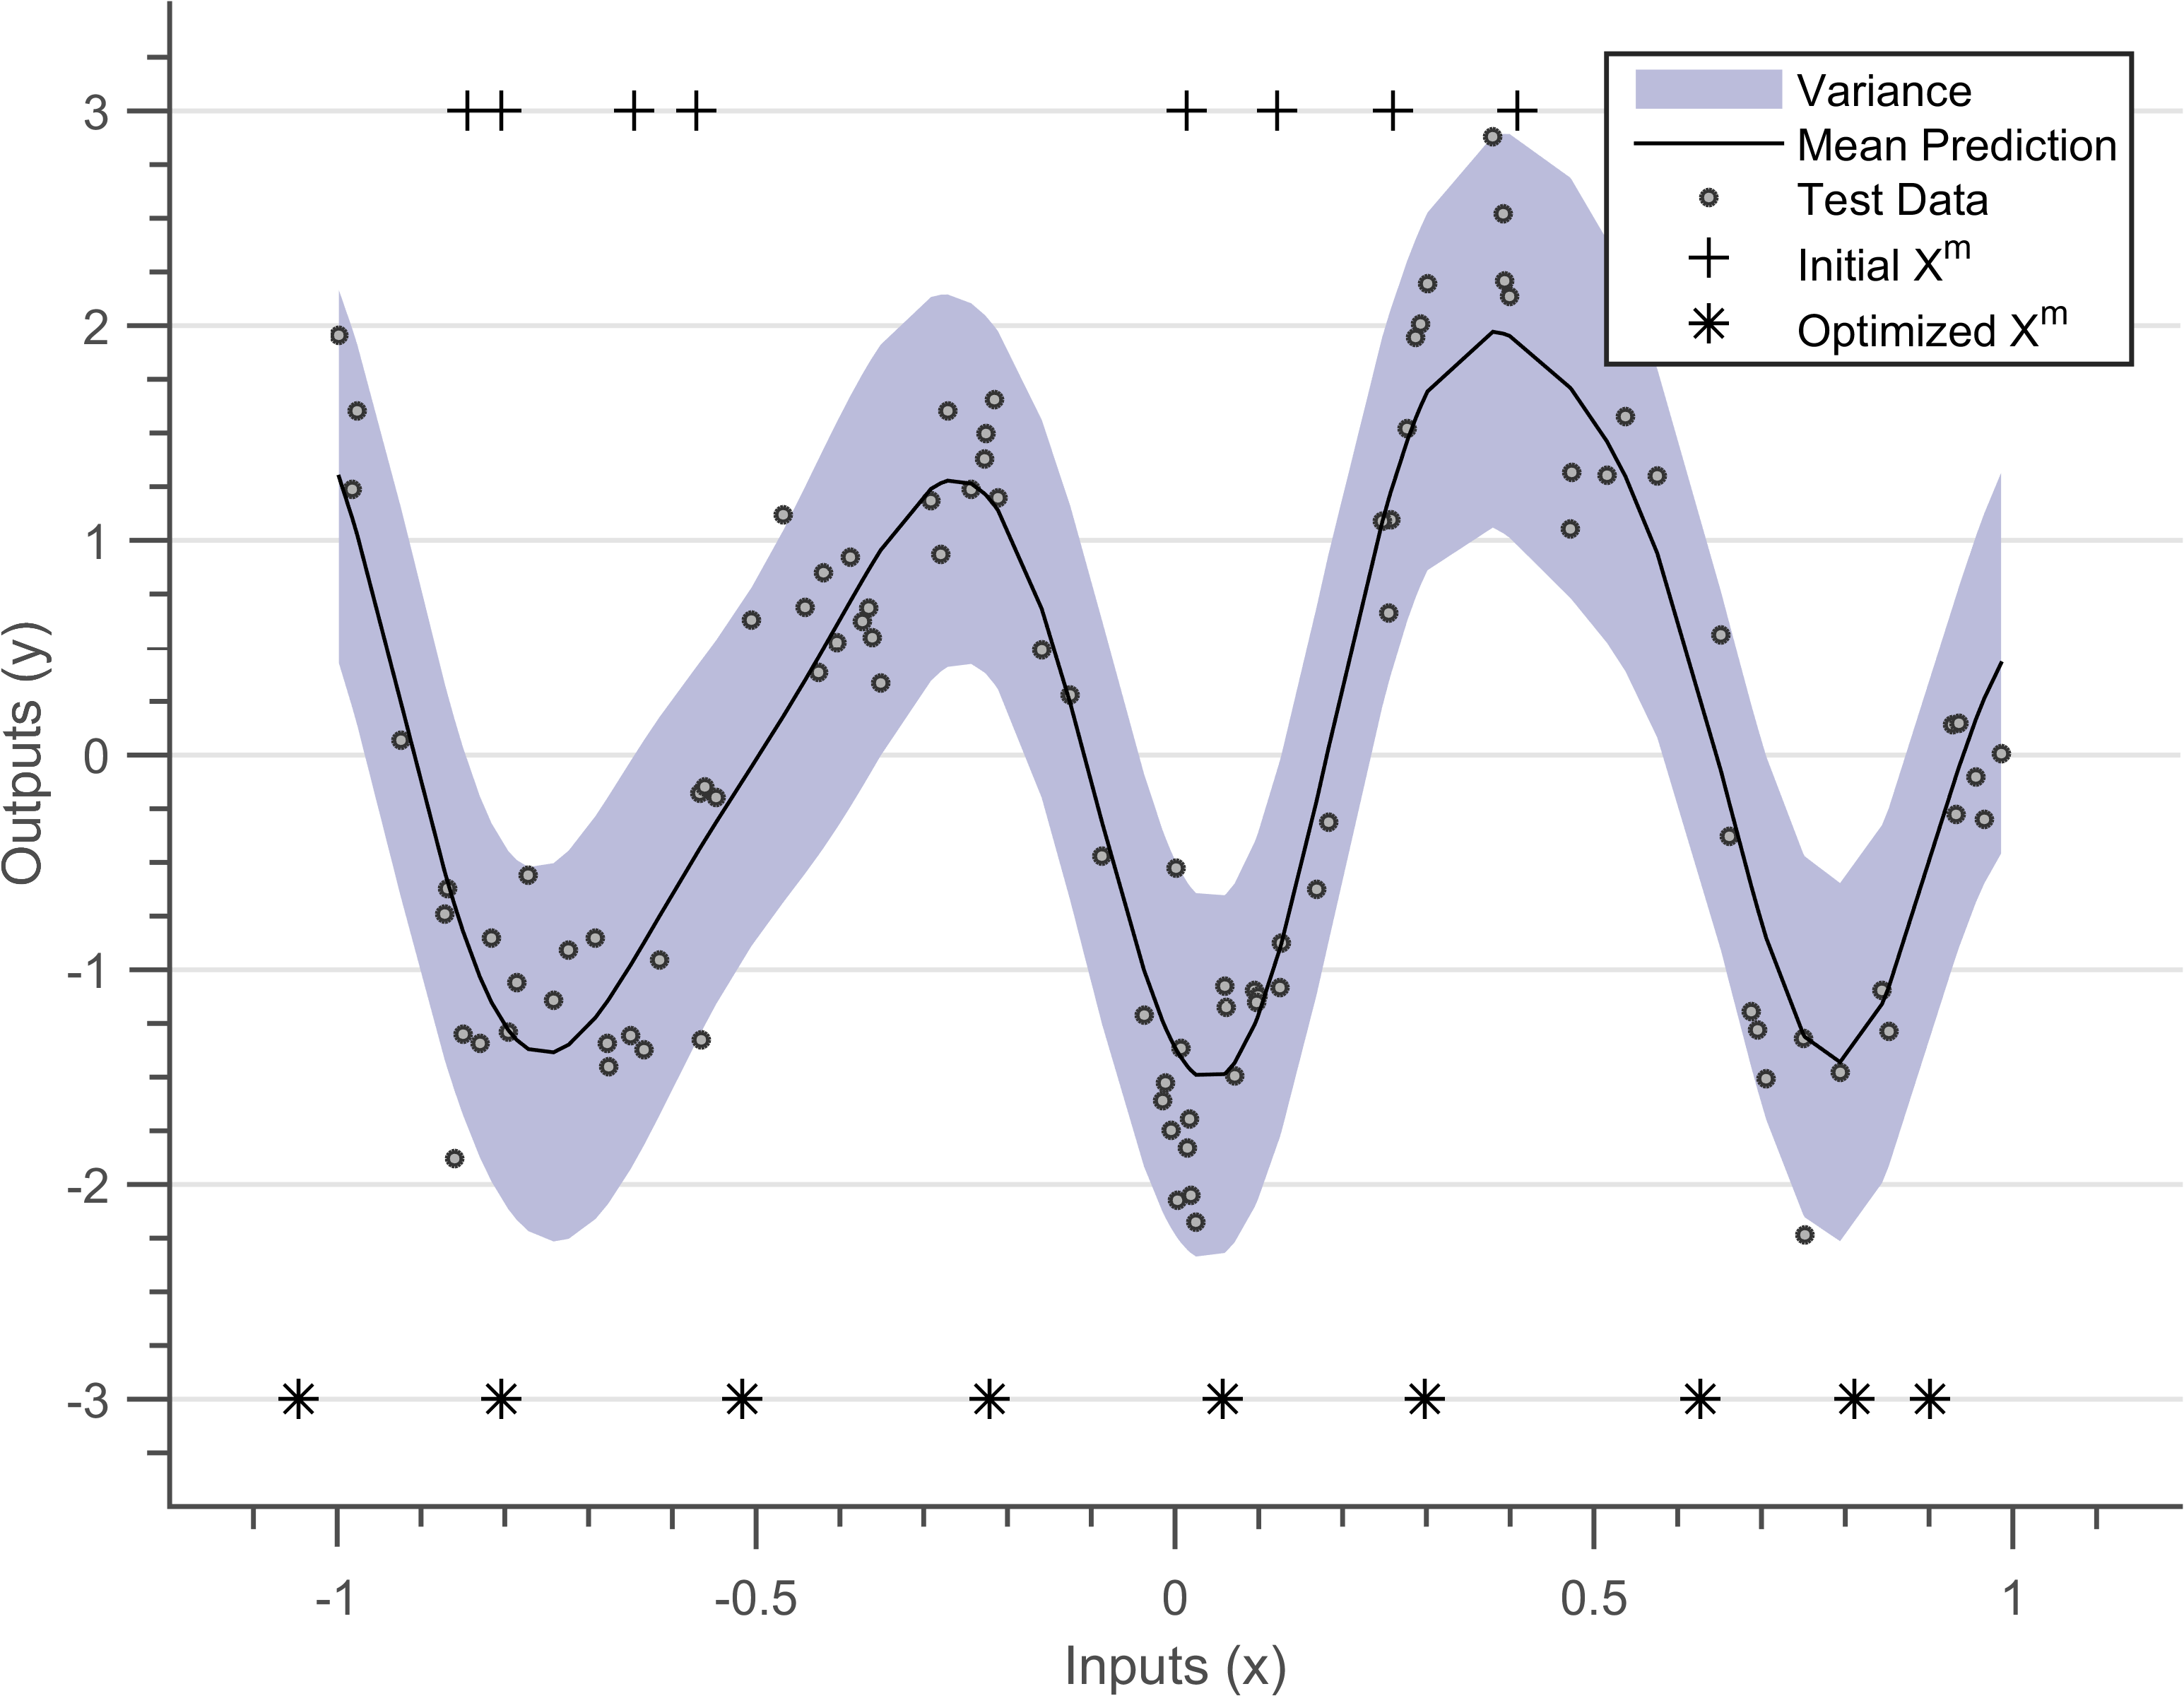
\includegraphics[width=0.45\textwidth]
        {images/part1/predictionOfm10_242}
        \label{predictionOfm10_242}
  }\quad
\subfigure[{10-fold RMSE box-plots for varying number of inducing points. The box-plots in red are cases when only the hyper-parameters $\theta$ were optimized while inducing inputs were distributed randomly. The box-plots in blue are the cases when both locations of inducing points $X^{m}$ and hyper-parameters $\theta$ are optimized. }]
  {
        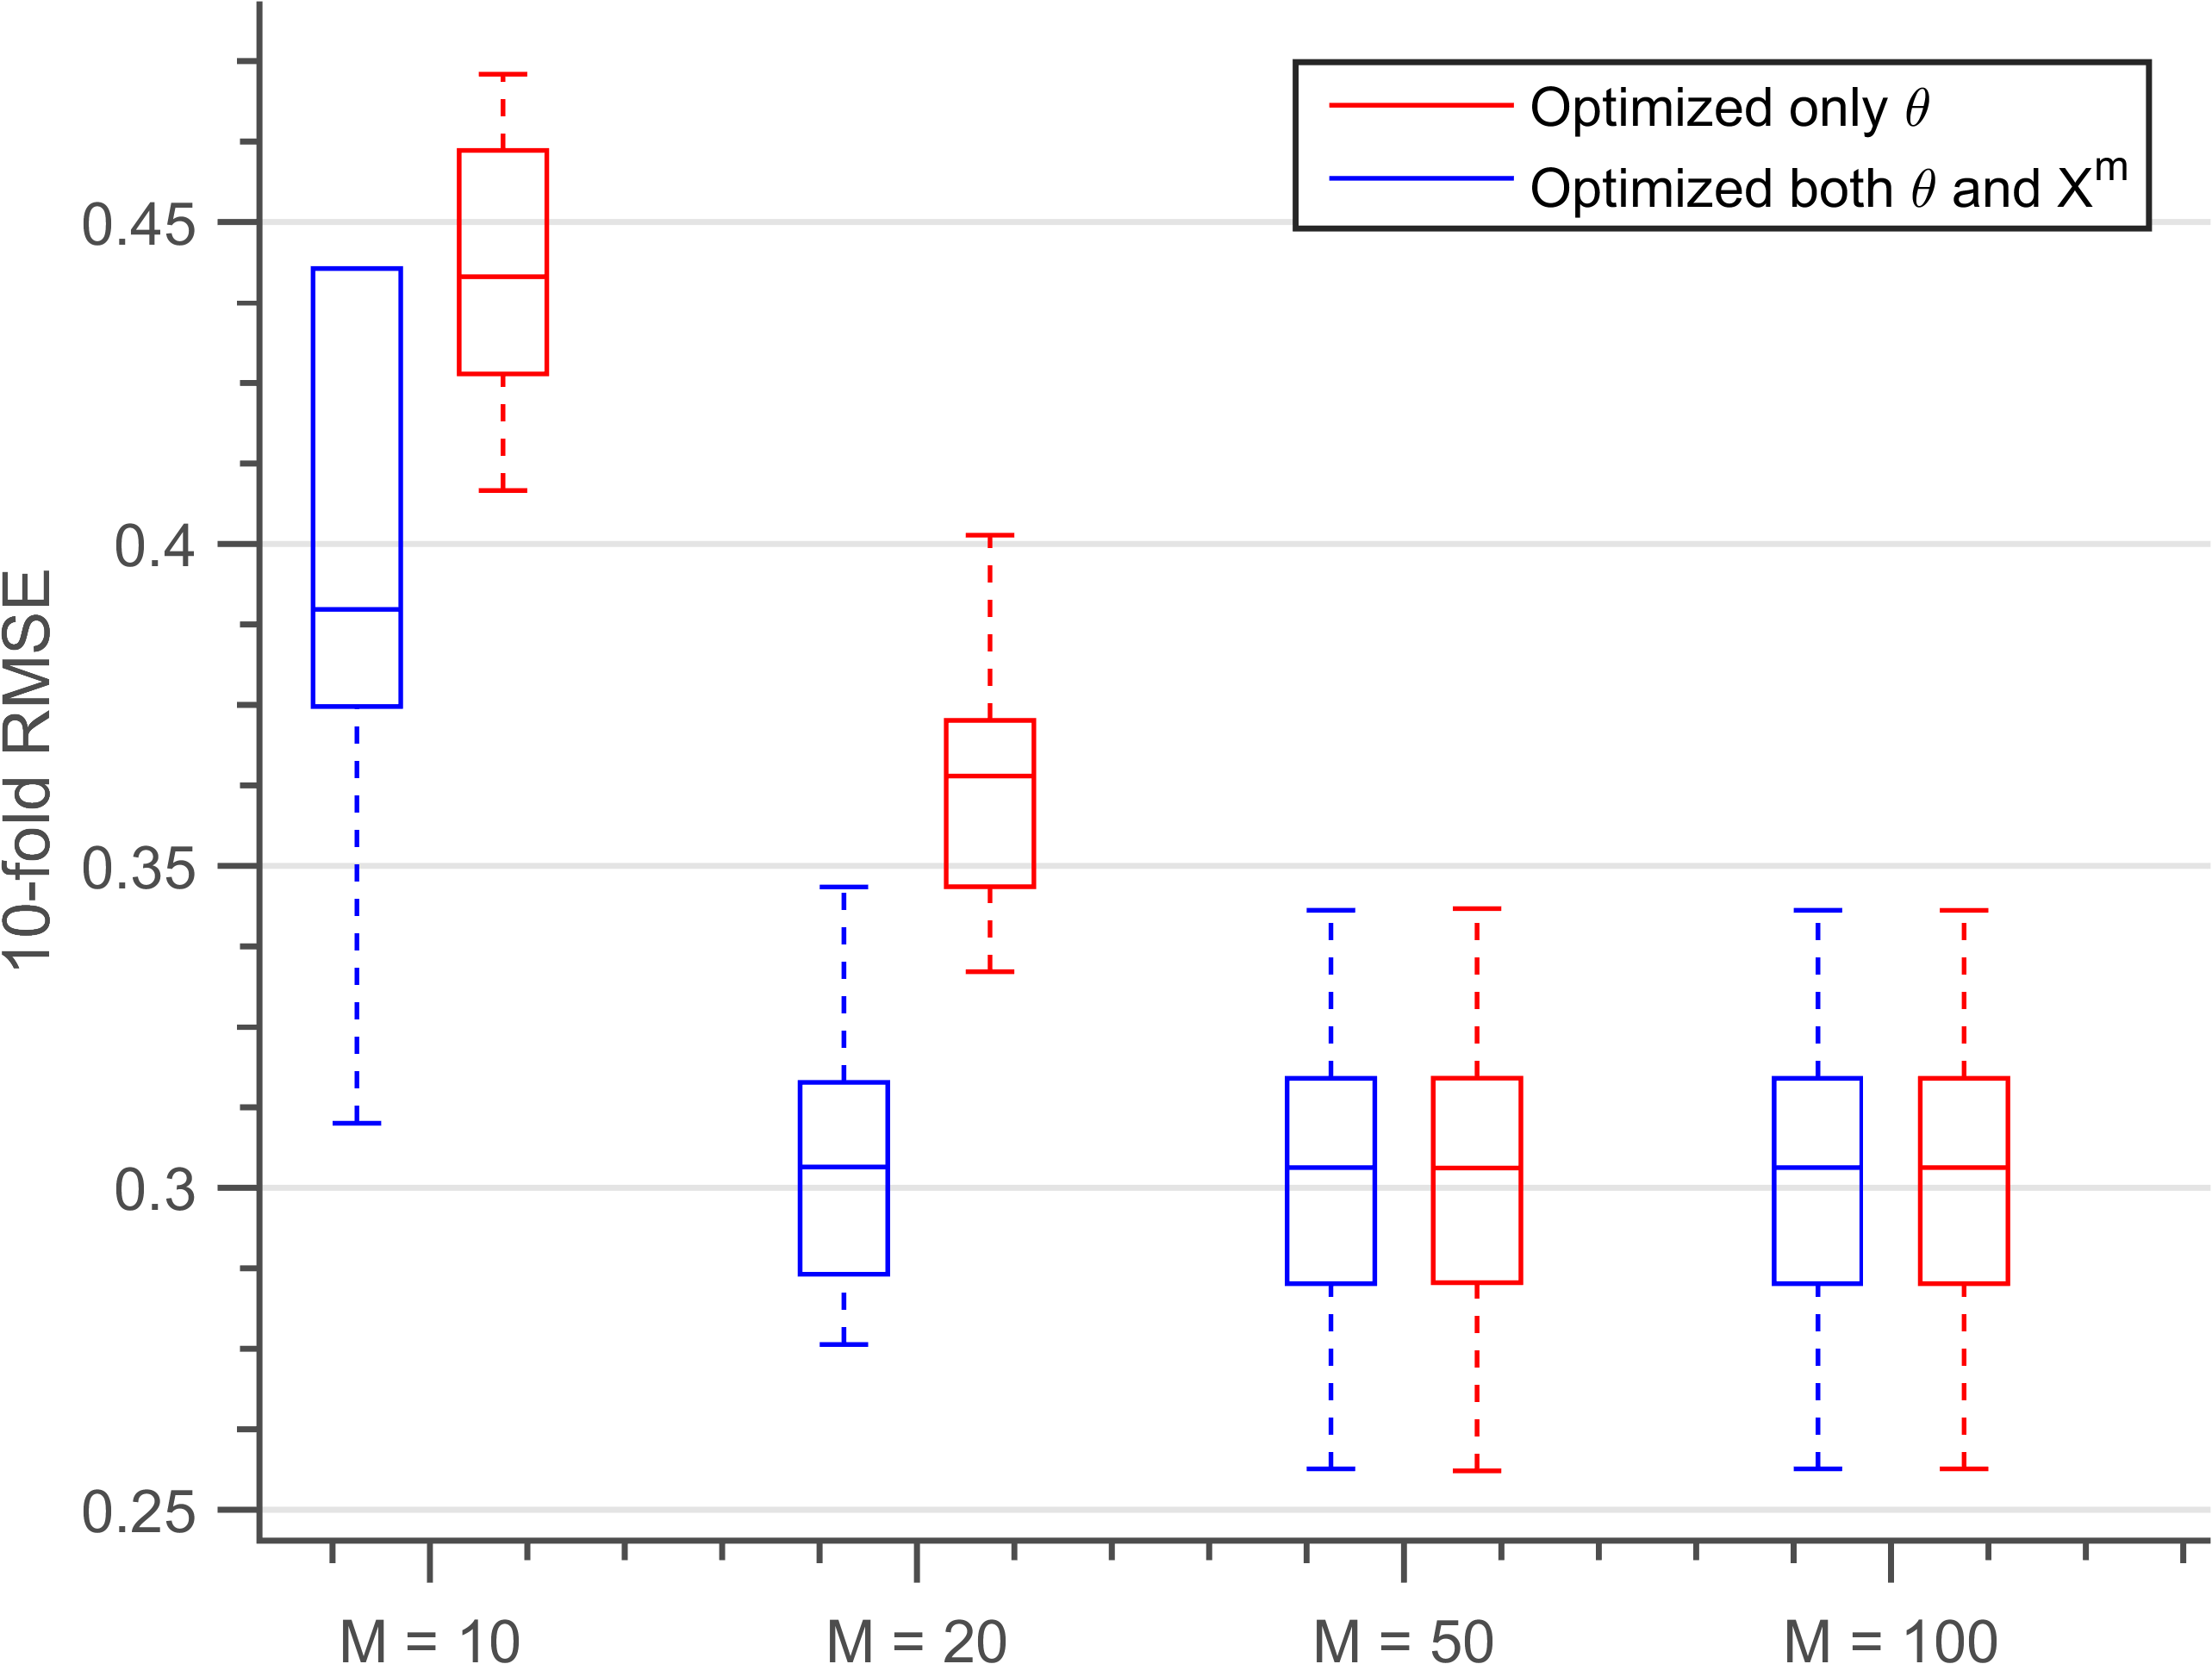
\includegraphics[width=0.45\textwidth]
        {images/part1/boxPlotsOfPerformance_242}
        \label{boxPlotsOfPerformance_242}
  }\quad
  
       \caption{Results of Nystr\"{o}m Approximation on a toy-data set of size $N=1000$ }\label{figGPPredictionNystorm}
\end{figure}

Global low-rank approximations are best suited for the case of spread out Gram matrices (example high length-scale SE priors). We have seen three types of low-rank approximation algorithms in this section. While Nystr\"{o}m and FITC approximations are the simplest method to approximate Gram matrix, finding optimal locations of the inducing points can often lead to over-fitting. We then, look at variational approximation procedure which adds a regularization term while finding inducing points thereby penalizing over-fitting. The lower computational cost due to sparse approximations, scales sparse GPs to the training set of sizes $N \sim \mathcal{O}(5 \times 10^5)$. \cite{Gal2014Distributed} propose a distributed architecture for scaling variational sparse GPs. In the next section we look at how to approximate Gram matrices using mixture of experts, this enables us to massively scale GPs to sizes $N > \mathcal{O}(10^6)$ by exploiting distributed architecture.

\section{Distributed Gaussian Process}\label{secDgp}
In the year 2006 Netflix prize was launched, teams from all over the world competed in the competition to make the best video recommendation algorithm. As the competition progressed teams figured out that performance increases upon combining algorithms developed by multiple teams. The winner and the runner-up were stacked learners of over 100 algorithms. Creating model ensembles (also called mixture of experts) is now a standard practice in many learning competitions \cite{bauer1998empirical}. 

Mixture of experts methods in GPs use bagging, where subsets of data are generated, individual GPs are trained on these subsets and their results are finally combined \cite{chen2009bagging}. If the data set is partitioned  into $N_{experts}$ subsets such as $\mathcal{D}^{(i)} = {X^{(i)}, Y^{(i)}}, i \in 1, \ldots N_{experts}$. Each subset of data learns an individual GP model, which can be combined together to give final predictions . Due to individual learning choosing hyper-parameters and calculating prediction become easily parallel-able and indifferent to the computational infrastructure. 

Initially, this mixture of local models was used to highlight local features in the data \cite{rasmussen2002infinite}. \cite{ng2014hierarchical} propose to use the mixture of experts methodology to speed up prediction in a GP. Instead of learning a different GP for each subset, we tie all the different experts using one single set of hyperparameters. This is equivalent to assuming one single GP for the whole data-set such that there is no correlation across experts, i.e. the experts are independent of each other. This tying of experts greatly reduces the number of hyper-parameters to optimize, acts as a regularization and inhibits over-fitting. Equation \ref{distributedGPPrior} denotes an independent GP prior for each expert $\mathcal{D}^{(i)}$ such that the hyper-parameters $\theta$ and $\sigma_{n}$ are same for all experts.

\begin{equation}\label{distributedGPPrior}
    \Pr[y^{(i)} \mid x^{(i)}, \theta, \sigma_{n}] = GP(0, K(x^{(i)}, x^{(i)'}, \theta) + \sigma^{2}_{n}I) 
\end{equation}

\textbf{comment about the algorithm}
\begin{mdframed}[hidealllines=true,backgroundcolor=lightgray!20]
\lstinputlisting[caption={Randomly clustering points into experts}, 
                    captionpos=b, 
                    label={codeClusteringIntoExperts}, 
                    backgroundcolor = \color{MatlabCellColour},
                    style=Matlab-editor]
                    {codes/chapter3/clusteringPointsInExperts.m}
\end{mdframed}

Figure \ref{subFigdistributedKernelRandomExperts} is an approximate Gram matrix using distributed GP approximation for a Standard Exponential (SE) Kernel with $(\theta = [1, 0.2])$ (figure \ref{subFigcovSEmatrix_1}) at the input points $X^{*} = \{[0:0.02:1]\}$. 5 experts each having 100 points are chosen, points in the experts are distributed randomly, this gives the approximate Gram matrix scattered shape. Figure \ref{subFigDistributedKernel} is an approximate Gram matrix using distributed GP approximation of the matrix in figure \ref{subFigcovSEmatrix_1} and uniformly distributed experts. 5 experts each having 100 points are chosen, The first expert has first set of 100 points, the second expert has the second set of 100 points and so on. The Gram matrix with randomly chosen experts has a more global nature but lacks many high variance regions. The Gram matrix for uniformly chosen experts retains more local features. Inversion of this Gram matrix is an operation of complexity $\mathcal{O}(N_{experts}P^{3})$, where $P$ is the number of points in an expert.

\begin{figure}[!ht]
  \centering
    \subfigure[{Approximated Gram matrix using distributed GP approximation for a Standard Exponential (SE) Kernel with $(\theta = [1, 0.2])$ (figure \ref{subFigcovSEmatrix_1}) at the input points $X^{*} = \{[0:0.02:1]\}$. Points in the experts are distributed randomly, this gives the approximate Gram matrix scattered shape.}]
  {
        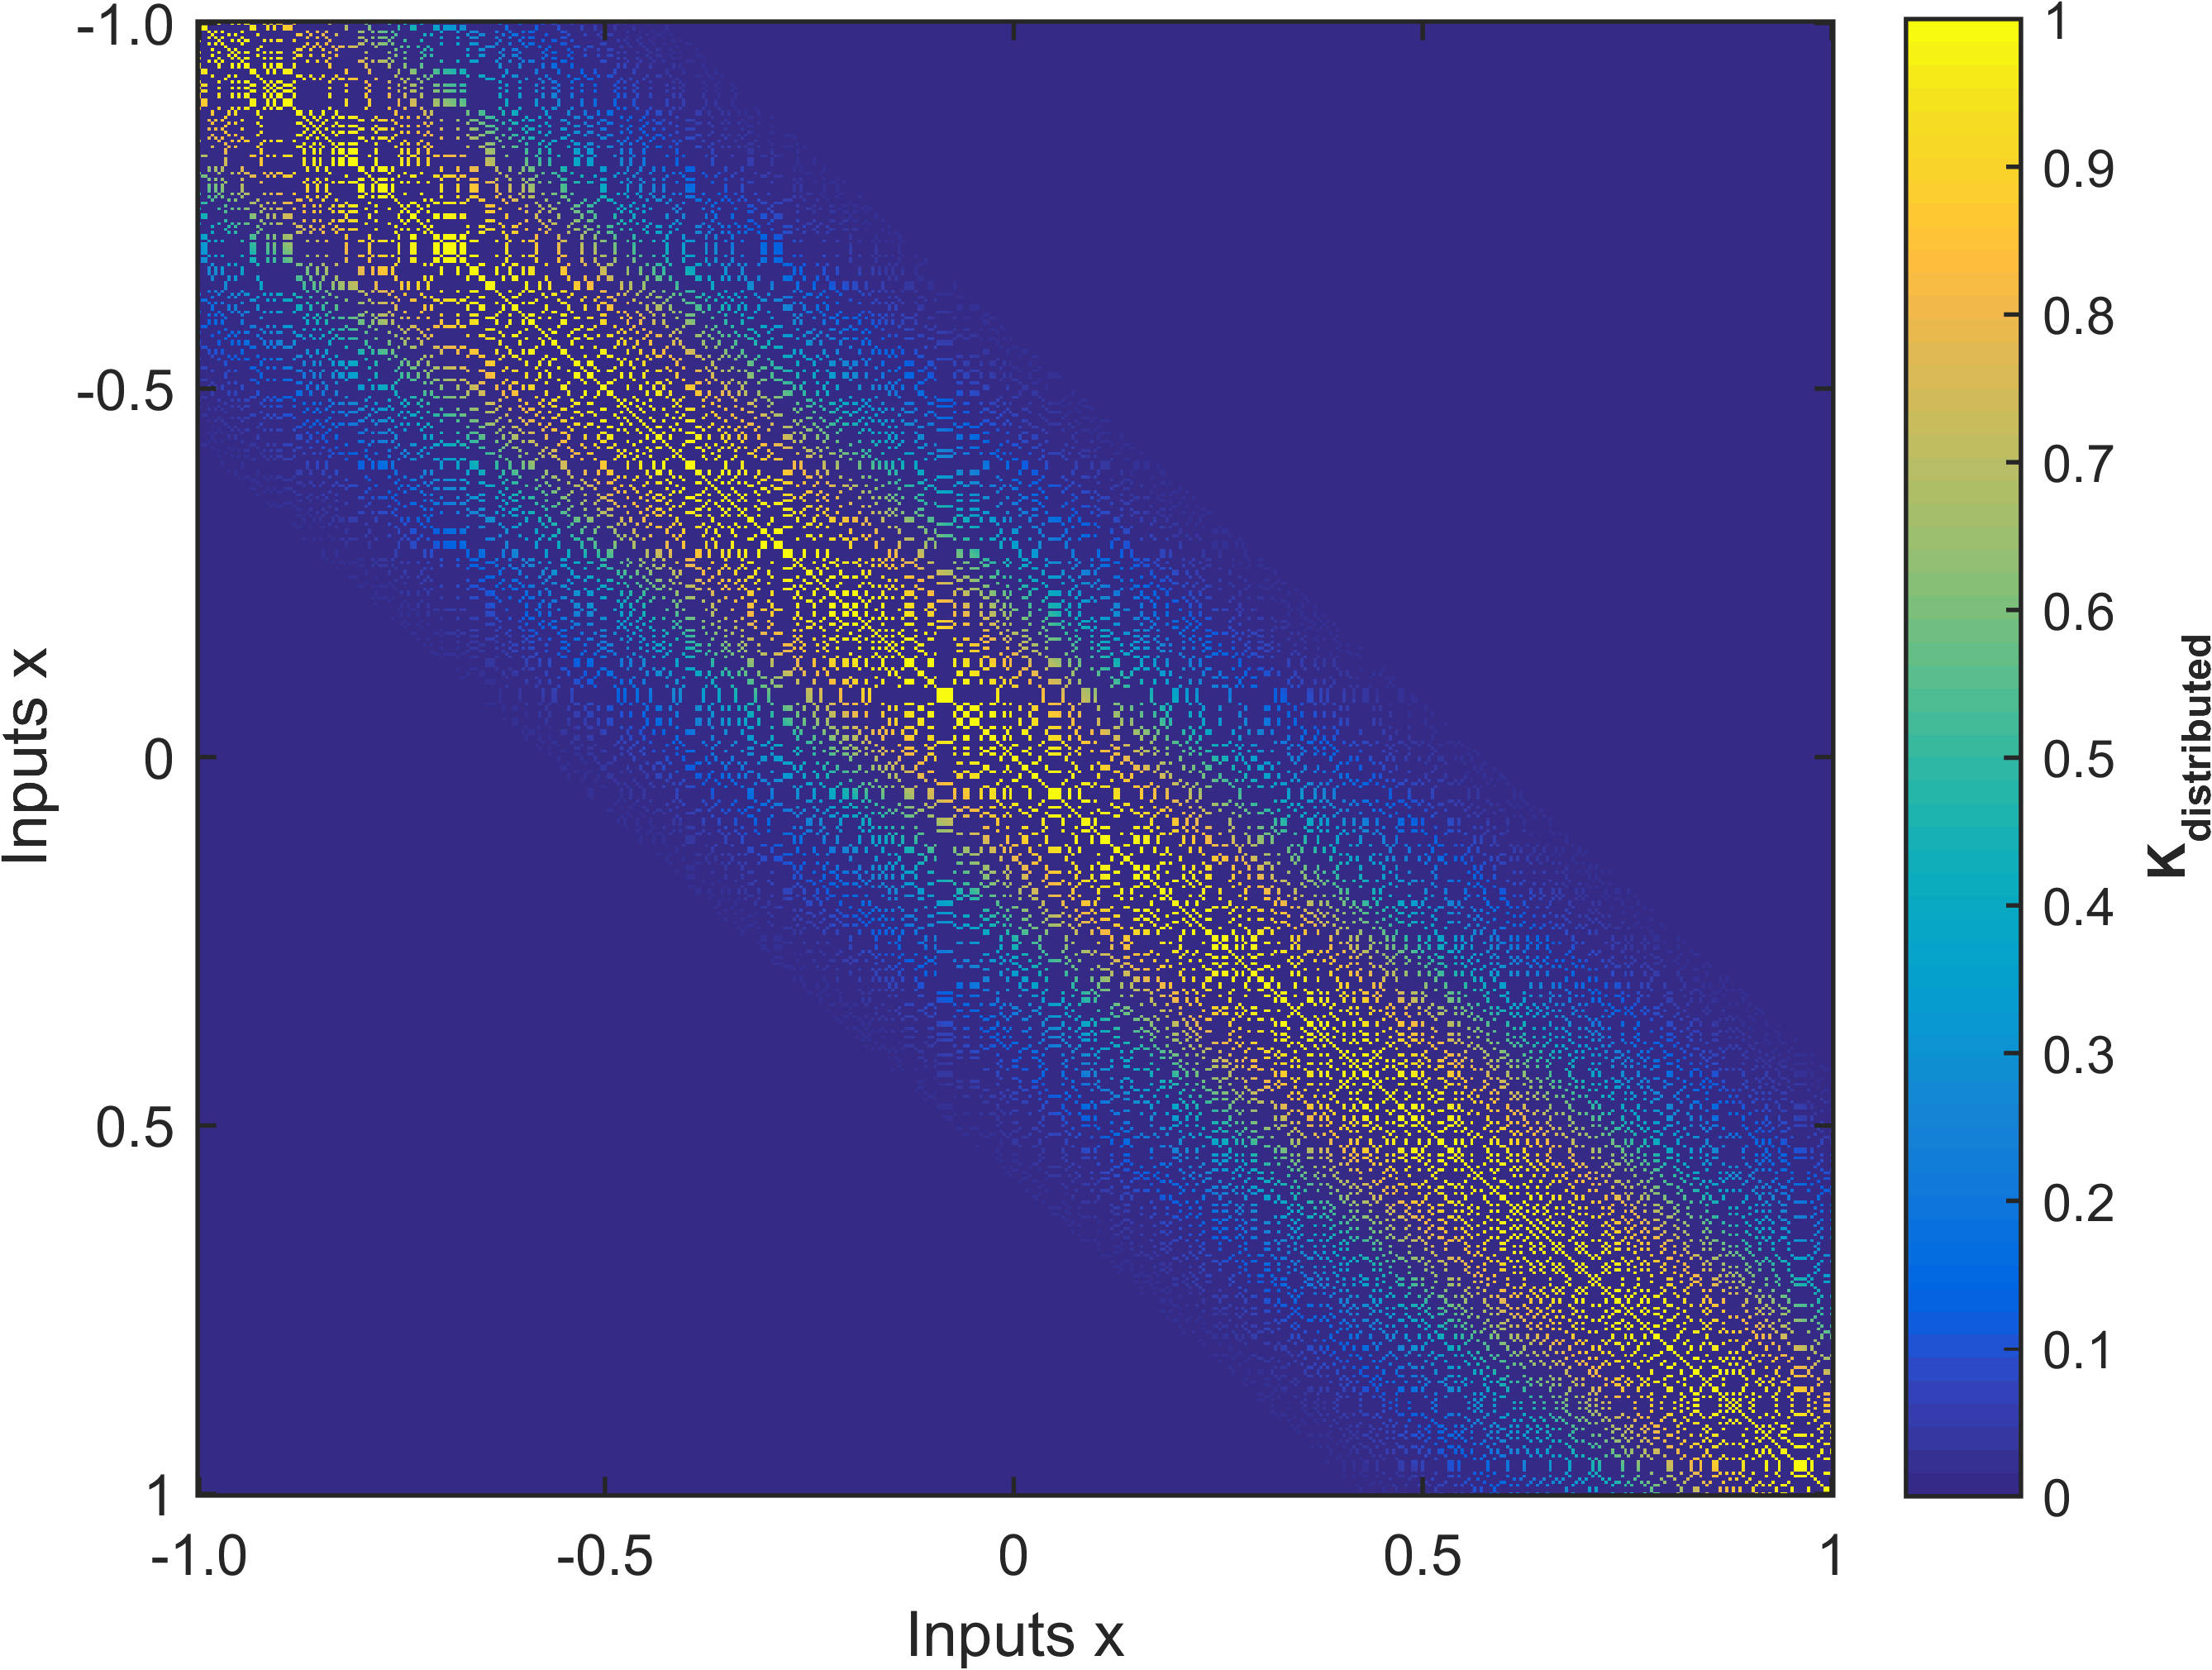
\includegraphics[width=0.45\textwidth]
        {images/part1/distributedKernelRandomExperts}
        \label{subFigdistributedKernelRandomExperts}
  }\quad
\subfigure[{Approximated Gram matrix using distributed GP approximation for a Standard Exponential (SE) Kernel with $(\theta = [1, 0.2])$ (figure \ref{subFigcovSEmatrix_1}) at the input points $X^{*} = \{[0:0.02:1]\}$. Points in the experts are distributed uniformly. We can observe that covariance across experts goes to zero.}]
  {
        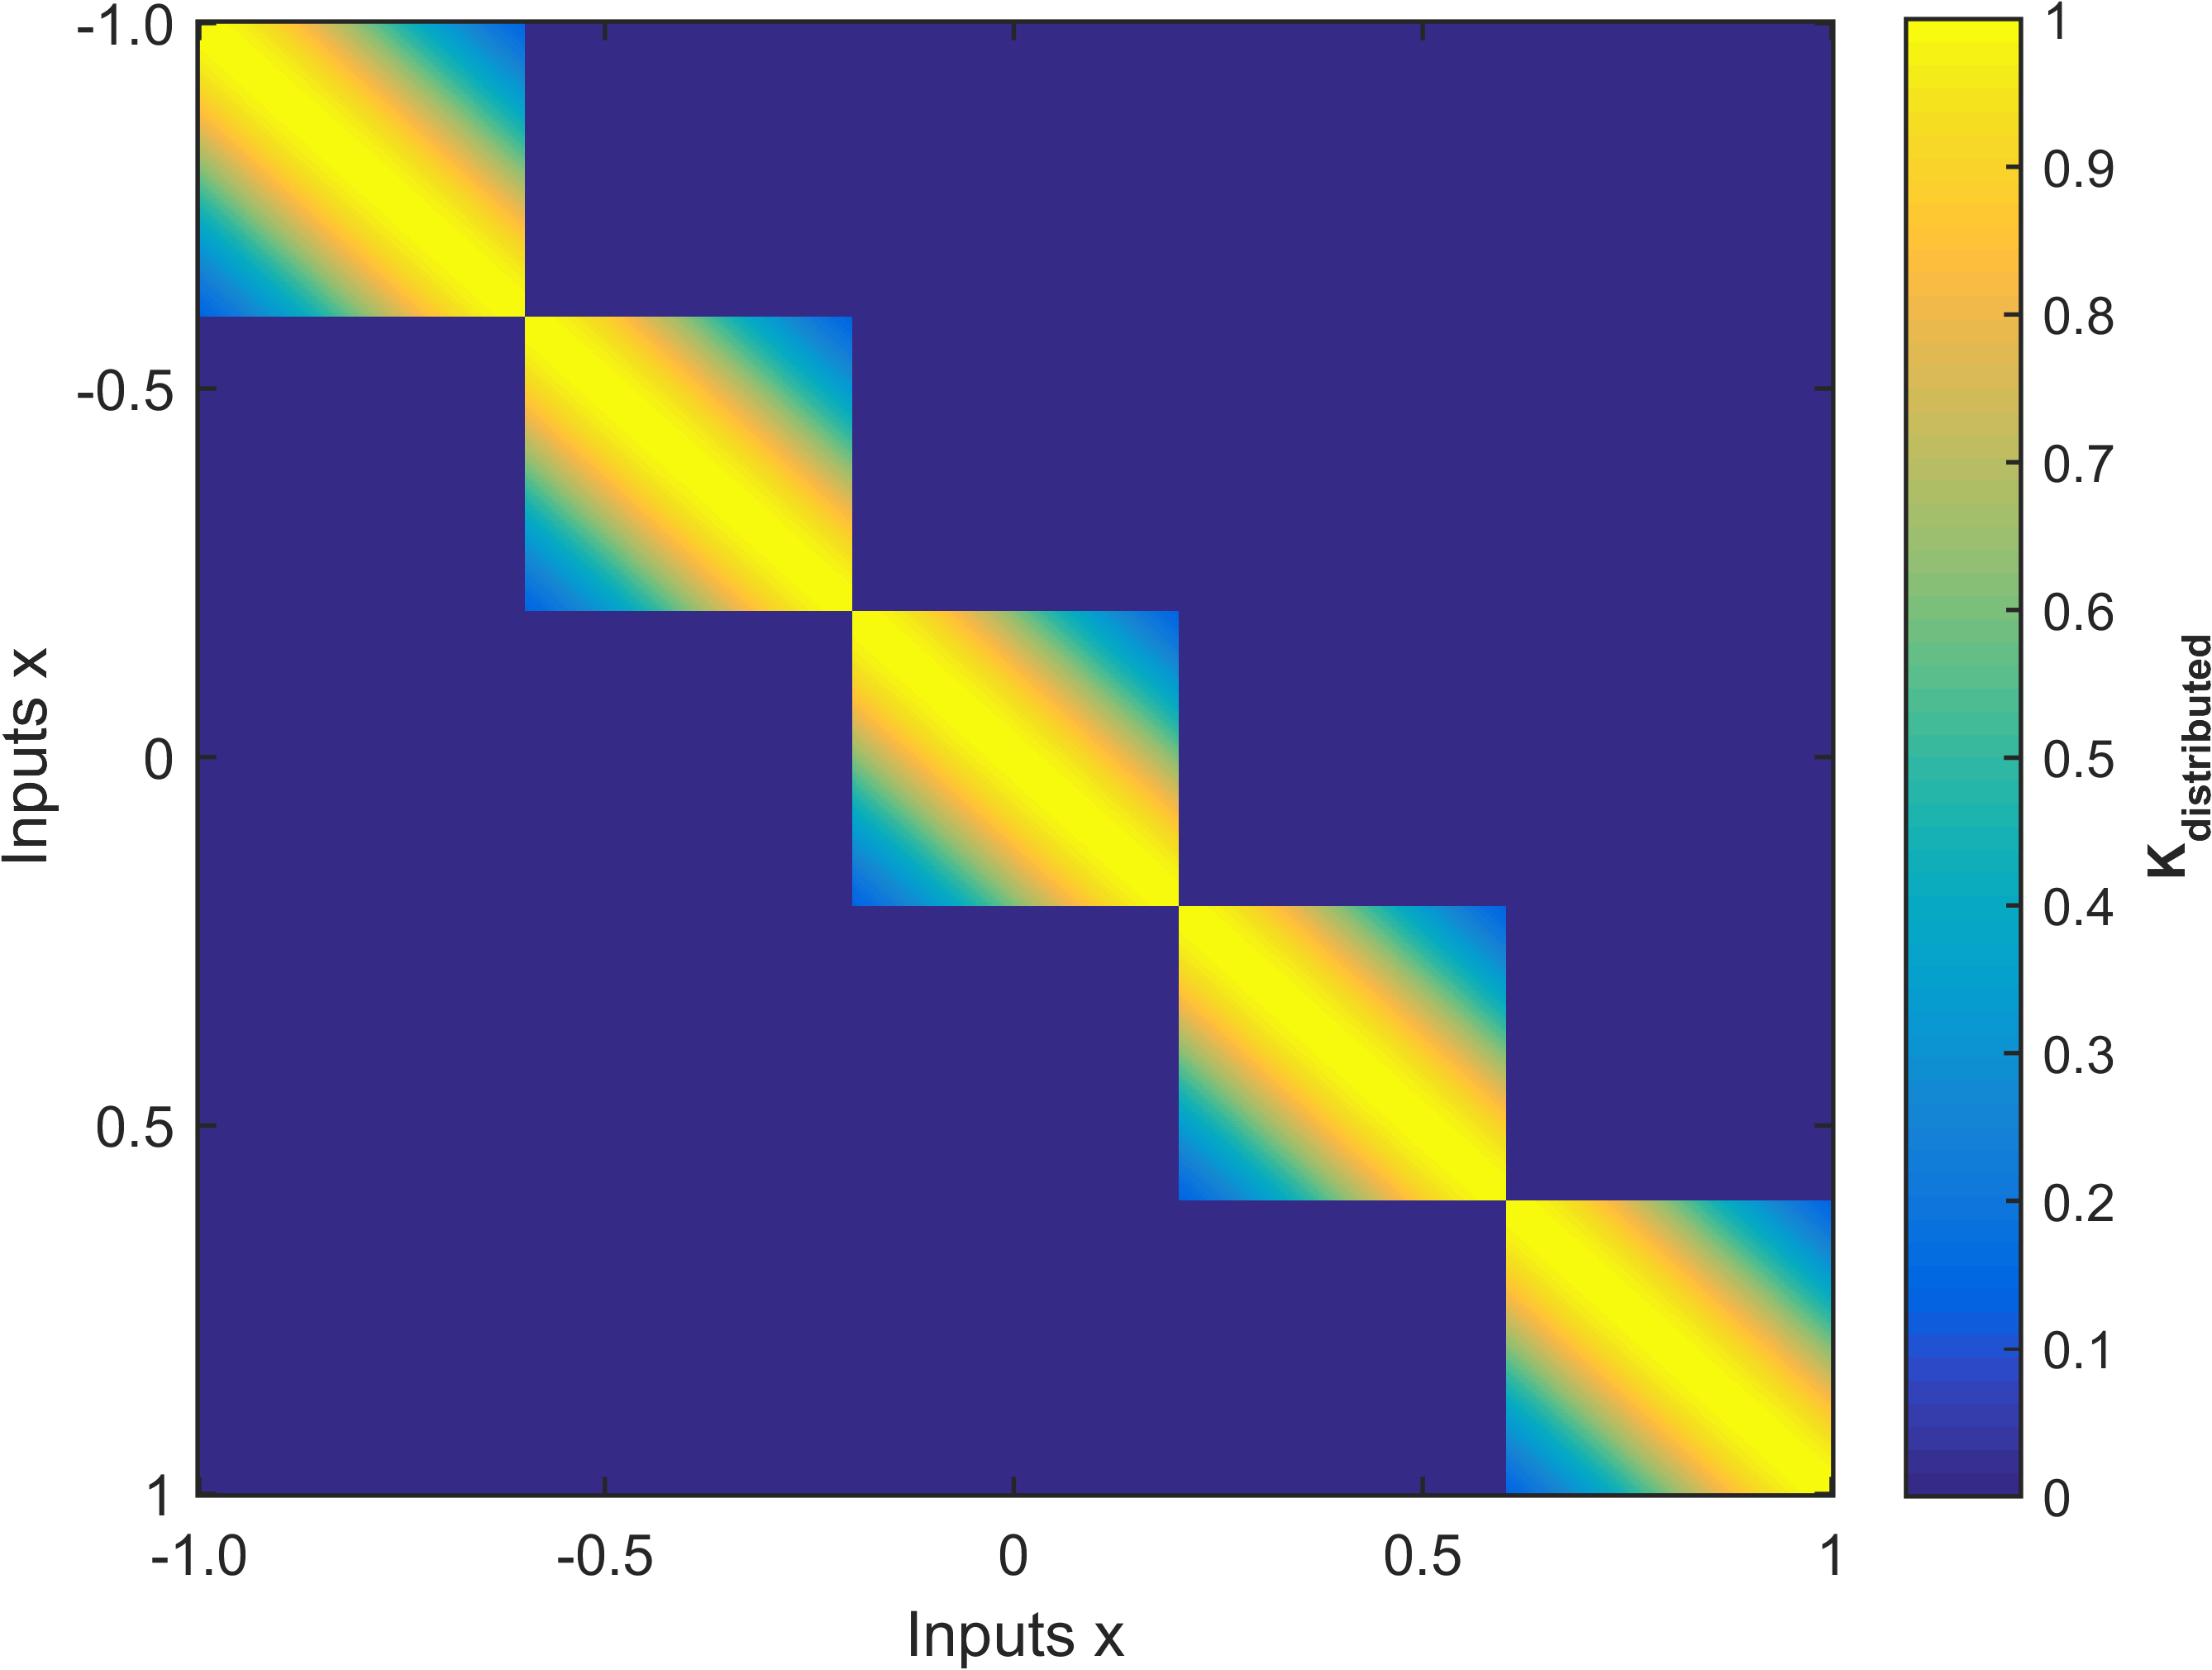
\includegraphics[width=0.45\textwidth]
        {images/part1/distributedKernel}
        \label{subFigDistributedKernel}
  }\quad
  
       \caption{Approximate Gram matrix for a Standard Exponential kernel using mixture of experts.}\label{figGPApproximateDGPMatrix}
\end{figure}

Since the experts are independent of each other, we can construct a posterior distribution for each expert (equations \ref{eqPredictiveMeanIndividualExpert} and \ref{eqPredictiveCovarianceIndividualExpert}). In the following equations $m^{(i)}(x_{*})$ and $\sigma^{(i)}(x_{*})$ are the mean and covariance predictions from expert $i$ at point $x_{*}$.  

\begin{equation}\label{eqPredictiveMeanIndividualExpert}
  m^{(i)}(y(x_{*})) = K_{x^{(i)}x_{*}}^{T}( K_{x^{(i)}, x^{(i)'}} + \sigma^{2}_{n}I)^{-1}y^{(i)}
  \end{equation}
\begin{equation}\label{eqPredictiveCovarianceIndividualExpert}
	\sigma^{(i)}(y(x_{*})) = K_{x_{*}x_{*}} - K_{x^{(i)}x_{*}}^{T}( K_{x^{(i)}, x^{(i)'}} + \sigma^{2}_{n}I )^{-1} K_{x^{(i)}x_{*}}
  \end{equation}

\subsection{Combining experts}\label{subSecCombiningExperts}
There exist several methods in the literature on how to combine these individual posterior predictions of the experts to give the final posterior distribution. The Product of Experts model uses the independence assumption between experts and multiplies the individual posterior distribution\footnote{$\Pr[y(x_{*}) \mid x_{*}, \mathcal{D}, \theta] \propto \prod \Pr[y^{(i)} \mid x^{(i)}, \mathcal{D}^{(i)}, \theta]$}, but these predictions tend to be overconfident. Another method called the generalized Product of Experts (gPOE) assigns a participation factor to each expert based on the amount of uncertainty in prediction (more confident experts have higher say in prediction)\cite{cao2014generalized}. The Bayesian Committee Machine (BCM) imposes the independence assumption between each expert pair using Bayes Rule, but can result in bad predictions when leaving data regime \cite{tresp2000bayesian}. 

This thesis will use robust Bayesian Committee Machine (rBCM) model to combine the posterior distributions of experts \cite{deisenroth2015distributed}. The rBCM model is an amalgamation of all the above three mentioned methods, it combines the confidence weighting parameter of gPOE with the Bayesian formulation in BCM technique to generate the following posterior distributions.

\begin{equation}\label{eqCovarianceDGP}
    Cov(y(x_{*}))^{^-2} = \sum_{i} \beta_{i}\sigma_{(i)}^{-2} + (1- \sum_{i} \beta_{i})(K_{x_{*}x_{*}})^{-2}
\end{equation}
\begin{equation}\label{eqMeanDGP}
    m(y(x_{*})) = (Cov(y(x_{*})))^{-2}\sum_{i} \beta_{i}(\sigma^{(i)})^{-2}m^{(i)}(x_{*})
\end{equation}

$K_{x_{*}x_{*}}$ is the auto-covariance of the prior at prediction point $x_{*}$. $\beta_{k}$ determines the influence of experts on the final predictions \cite{cao2014generalized} and is given as $\beta_{i} = \frac{1}{2}(\log K_{x_{*}x_{*}}^{2} - \log(\sigma^{(i)})^{2})$. Experts which are very confident of their predictions at $x_{*}$ will tend to have low $\sigma^{(i)}$ thereby leading to a higher influence factor $\beta_{i}$.

Due to the independence assumption, the marginal likelihood can be written as a sum of individual likelihoods and then can be optimized to find the best-fit hyperparameters. By approximating the $K(X, X)$ in terms of $\mathcal{D}^{(i)}$ and $N_{experts}$ we have again changed the GP prior. This means that the number of experts $N_{experts}$ and clustering of points in individual experts also impact the prediction capabilities of GP. The below equation \ref{eqDGPNLML} describes the formulation for marginal likelihood. 

\begin{align}\label{eqDGPNLML}
    \log \Pr[y \mid X, \mathcal{D}, \theta] \approx \sum_{k=1}^{N_{experts}} \log \Pr[y^{(i)}\mid X^{(i)}, \theta]
 \end{align}

\textbf{comment about the algorithm}
\begin{mdframed}[hidealllines=true,backgroundcolor=lightgray!20]
\lstinputlisting[caption={log Marginal Likelihood for Distributed GP}, 
                    captionpos=b, 
                    label={codelmdDGP}, 
                    backgroundcolor = \color{MatlabCellColour},
                    style=Matlab-editor]
                    {codes/chapter3/logMarginalLikelihoodDGP.m}
\end{mdframed}

Maximizing the above log-marginal likelihood will give the optimal values of hyper-parameters. Points in the experts can be distributed either randomly or using a clustering scheme (eg. k-means clustering\footnote{k-means algorithm clusters close by points in one cluster. The notion of closeness is defined by some measure of distance}) for stationary kernels\footnote{stationary kernels are only a function of $\tau = |x-x'|$} k-means clustering should be preferred. The k-means algorithm clusters points based on a measure of distance, points in separate clusters are far away from each other when compared to points in the same cluster. This means that the covariance (for stationary kernels) between separate clusters is significantly lower when compared to points in same cluster. Hence, the cross-covariance across separate clusters can be more easily assumed to be zero.

\subsection{Experiments}\label{subSecDistributedExperiments}
We again conduct experiments on a toy-data set, this time to observe the accuracy of distributed GP approximation for varying number of experts. 

Again the 10-fold Cross Validation (CV) will be used to assess the performance of the prediction. The same toy-data set as used in section \ref{subsecNystromExperiments} was used to perform the experiments in this section (1000 data-points from $\Pr[y \mid X, \theta, \sigma_{n}] = GP(0, K_{SE}(X, X', \theta = [1, 0.1]) + (0.3)^{2}I)$.

Figure \ref{predictionOfm10_243} is the prediction of the GP obtained after distributed approximation using 9 experts and k-means clustering. The solid black line defines the mean function, blue region defines 95\% confidence interval (2$\sigma$) distance away from the mean. The colored points in the points denoted by `*' at the bottom show how different points are distributed across experts, similar colored points belong to one expert. The data denoted by `.' is the test data for one fold of the 10-fold CV. 

The points across experts are uniformly distributed, as can be observed by the coloring scheme. Since the training points are almost uniformly distributed, the k-means algorithm will cluster the points uniformly. Actually, the training and test set used in figures \ref{predictionOfm10_243} and \ref{predictionOfm10_242} are same. Notice how Nystr\"{o}m approximation has a global smooth shape while the distributed GP approximation retains the local features of the data set. 

Figure \ref{boxPlotsOfPerformance_243} are 10-fold RMSE box-plots for different number of $P$. The box-plots in red are cases when the points are distributed using k-means clustering. The box-plots in blue are the cases when points are distributed randomly. The accuracy of prediction improves with increasing number of points in an expert. Note, the noise in the generated toy-data is $\sigma_{n}=0.3$, hence $0.3$ is the best achievable RMSE value. Accuracy is slightly better when experts are distributed using k-means clustering, both being very close to the $0.3$ RMSE limit. As a thumb-rule setting $P = N/10$ and optimizing the hyper-parameters ($\theta$) is a good enough approximation. 


\begin{figure}[!ht]
  \centering
    \subfigure[{Prediction of the GP obtained after distributed approximation using 9 experts and k-means clustering. The solid black line defines the mean function, blue region defines 95\% confidence interval (2$\sigma$) distance away from the mean. The colored points in the points denoted by `*' at the bottom show how different points are distributed across experts, similar colored points belong to one expert. The data denoted by `.' is the test data for one fold of the 10-fold CV. }]
  {
        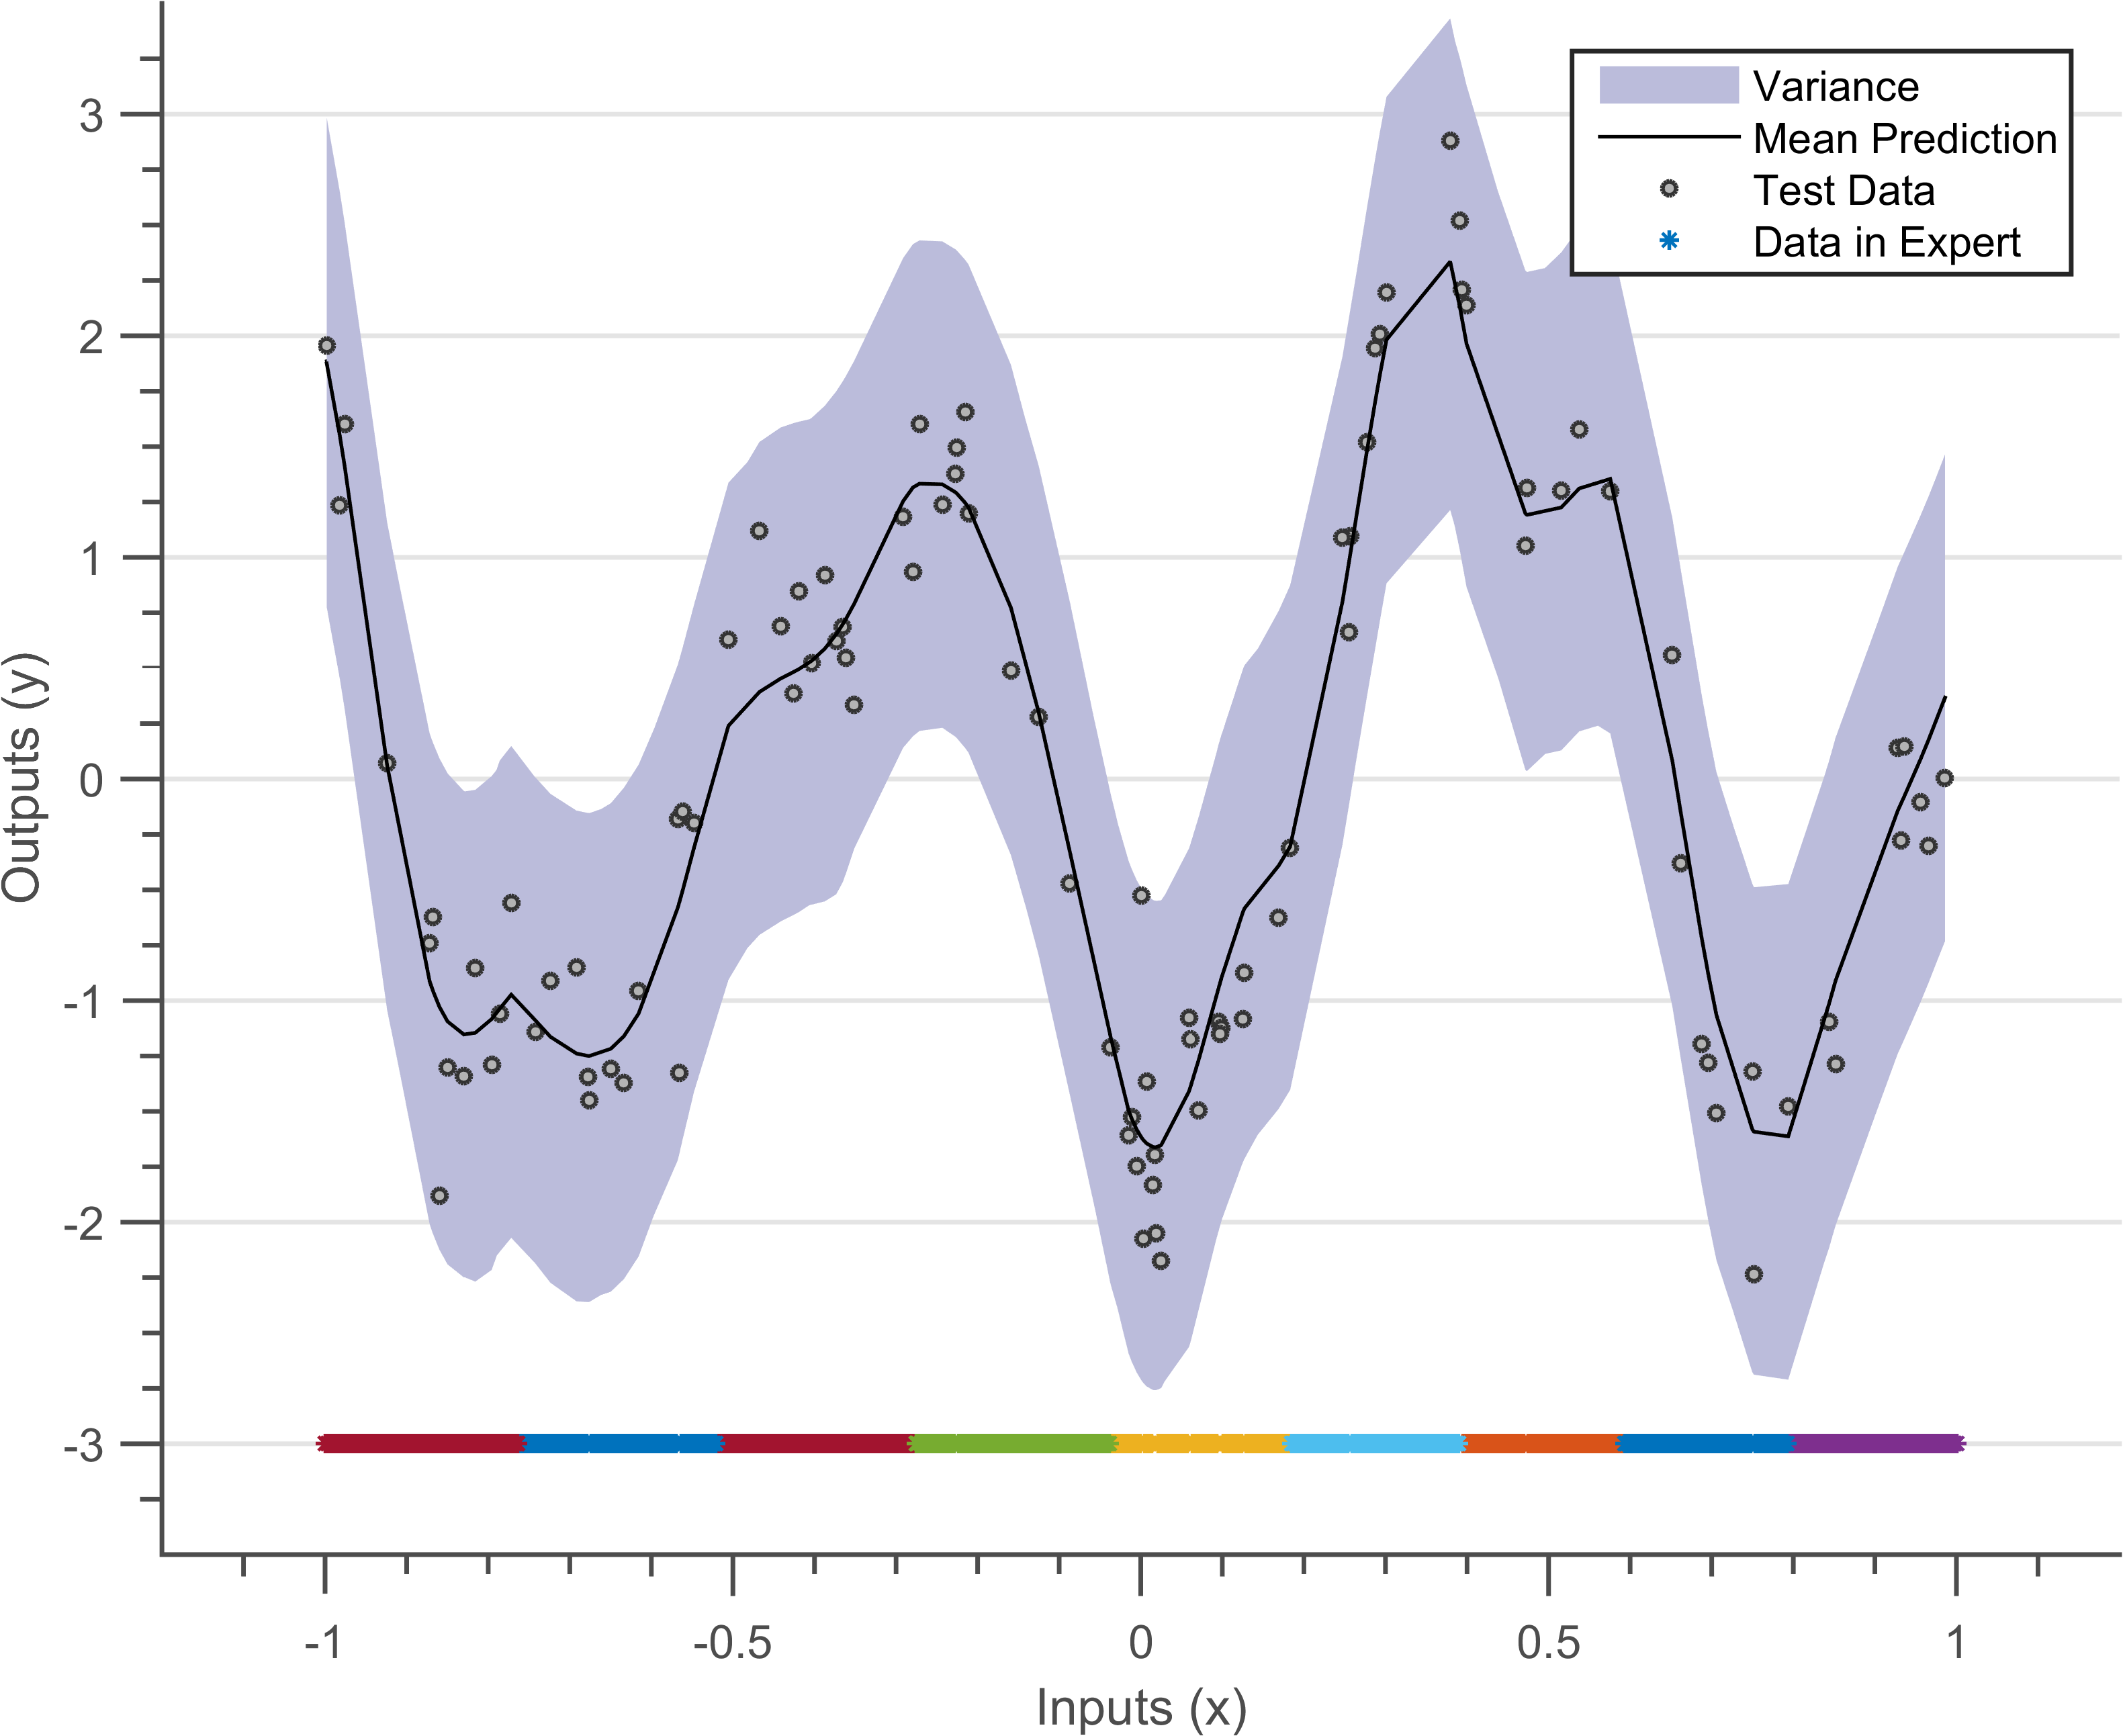
\includegraphics[width=0.45\textwidth]
        {images/part1/predictionOfm10_243}
        \label{predictionOfm10_243}
  }\quad
\subfigure[{10-fold RMSE box-plots for different number of points across. The box-plots in red are cases when only the hyper-parameters when the points are distributed using k-means clustering. The box-plots in blue are the cases when points are distributed randomly. The accuracy of prediction improves with increasing number of points in an expert}]
  {
        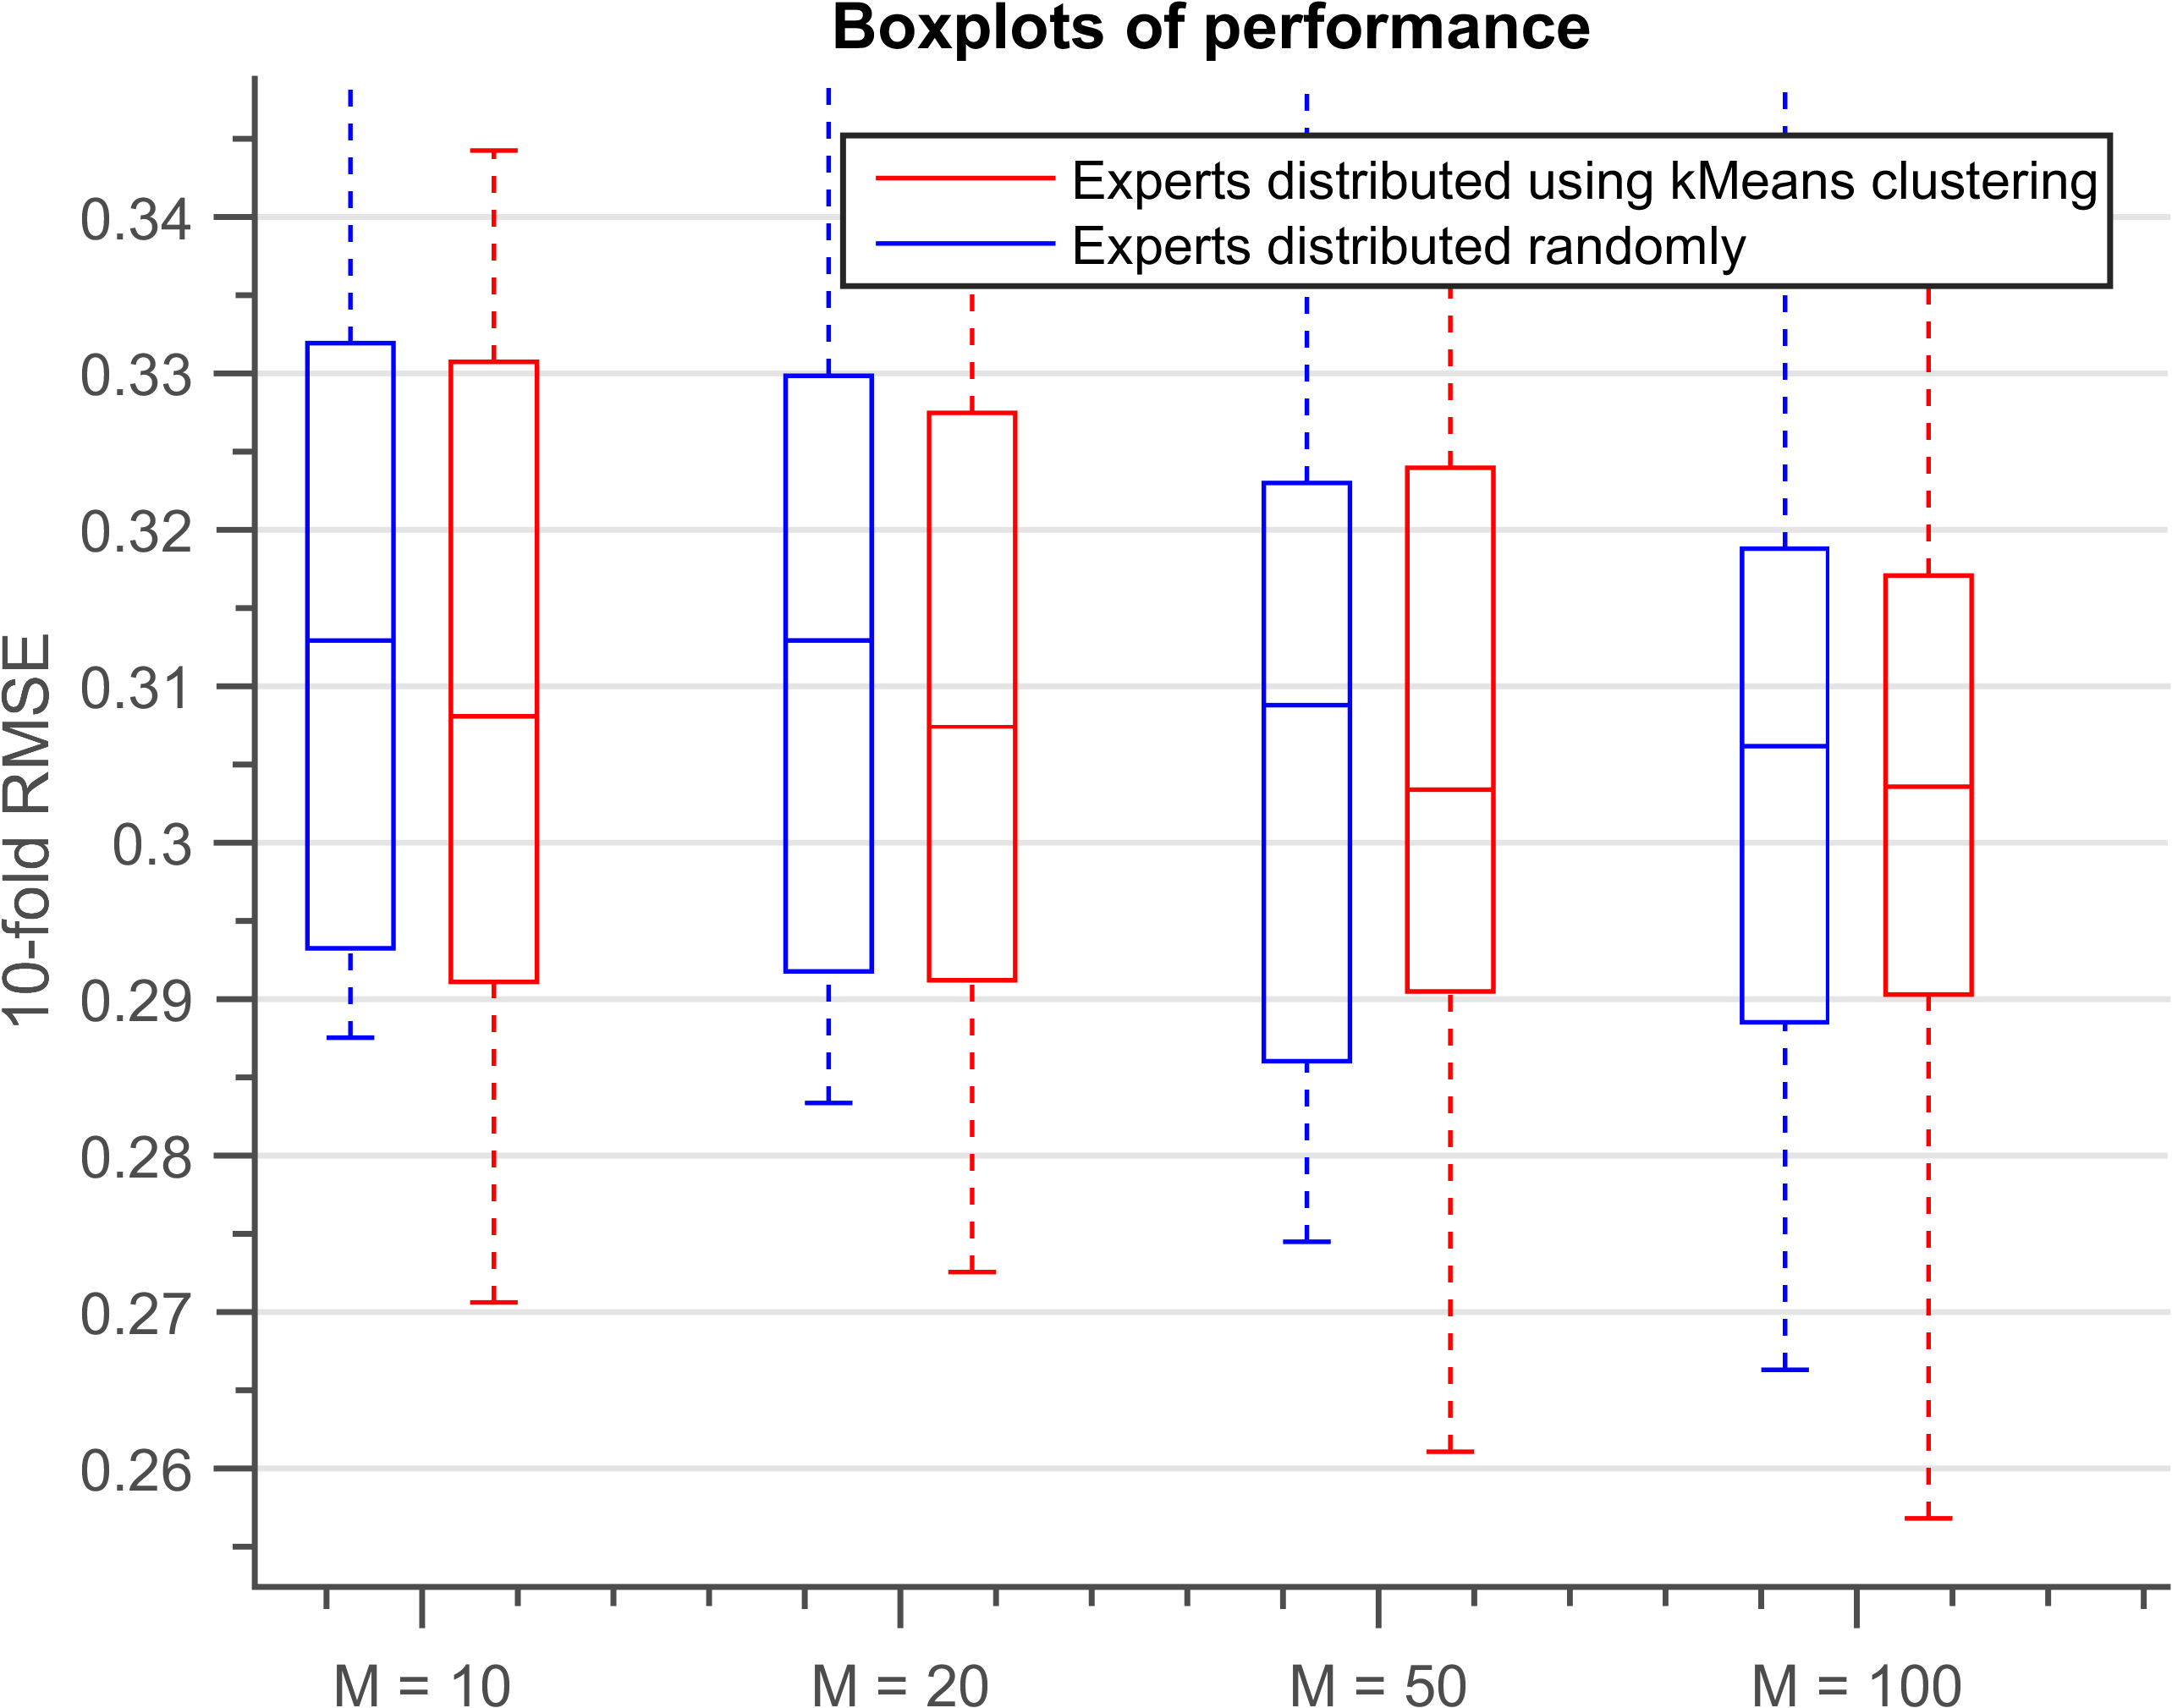
\includegraphics[width=0.45\textwidth]
        {images/part1/boxPlotsOfPerformance_243}
        \label{boxPlotsOfPerformance_243}
  }\quad
  
       \caption{Results of distributed GP Approximation on a toy-data set of size $N= 1000$}\label{figGPPredictionDistributed}
\end{figure}

\section{Discussion}
The calculation of posterior distribution in GPs becomes computationally intractable for large data sets. Calculating the precision matrix is an operation of computational complexity $\mathcal{O}(N^{3})$, putting a limit of $N \sim 10^4$ data points for model building. This chapter describes the state of art for scaling up GPs for regression tasks. There exist two methods to scale up GPs, the first called sparse methods which uses a set of inducing inputs to reduce the computational cost of calculating the precision matrix. The second called distributed GP which divides the data set into another set of smaller datasets called experts, distributing the model building into several batches. 

Sparse methods use Nystr\"{o}m approximation rewriting the Gram matrix as equation \ref{subSecSamplingFunctionsGPPrior}, thereby reducing the computational complexity to $\mathcal{O}(NM^{2})$ (M << N), $M$ being the number of inducing points. Through experiments on a toy-dataset it can be shown that we can set $M \sim N/10$ for randomly distributed inducing points and $M \sim N/50$ when we optimize the locations of inducing points. This approximation pushes the limit of GP Regression to $N \sim 10^6$ data points. Distributed GPs distributes the GP Regression tasks into several batches, thereby reducing the computational complexity to $\mathcal{O}(NP^{3})$ (P<<N), $P$ being the number of points in an expert. Through experiments on a toy-dataset we demonstrate that $P \sim N/100$ does not effects the regression task significantly. In fact we can further reduce $P$ if we enable repetition of points between experts. This enables to scale GPs to any number of data-points, we will demonstrate this by running a GP regression on millions of data-points in this manuscript (section \ref{chapCombiningBasicCovariances}). 

There are several reasons why GPs should be preferred to perform regression tasks. GPs provide a probabilistic framework to define a family of functions, while the covariance functions allows to incorporate a wide range of assumptions (Chapter \ref{chapBasicCovarianceKernels}). GPs are computationally tractable, given a covariance function and observations, the predictive distribution can be calculated exactly. By providing a closed form expression of marginal likelihood GPs provide a powerful method to automatically select hyperparameters. Although GPs suffer in presence of large data sets, there exist several approximate methods to scale GPs to millions of data points. 






\part{Incorporating structure in Gaussian Process Regression}\label{partIncorporatePattern}
\include{2-chapters/2-II-overview}
\chapter{Basic Covariance Functions}
\label{chapBasicCovarianceKernels}

\begin{mdframed}[hidealllines=true,backgroundcolor=lightgray!20]
\section*{Résumé}
La partie \ref{partIncorporatePattern} de la thèse montre comment incorporer les informations \textit{a priori} dans la construction de modèles GP, en choisissant les différents types de fonctions de covariance. Bien que les formes fonctionnelles de covariance discutées ici soient généralement utilisées dans la communauté d'apprentissage automatique, elles ne sont pas souvent utilisées pour construire des modèles d'ingénierie. La contribution originale du chapitre \ref{chapBasicCovarianceKernels} et du chapitre \ref{chapCombiningBasicCovariances} est l'application de ces noyaux pour construire des modèles d'ingénierie (en mécanique des fluides et en structure). Cette partie est fortement inspirée des travaux aux \cite{duvenaud-thesis-2014, wilson2014thesis, lloyd2014automatic, durrande2001etude}.

La Section \ref{secPropertiesOfCovariance} définit quelques propriétés importantes des fonctions de covariance. La Section \ref{secNonStationaryKernels}  détaille quelques propriétés de noyaux non-stationnaires et discute dans quelle mesure la Régression Linéaire Bayésienne peut être efficacement vue comme une régression GP avec la fonction de covariance linéaire. La Section \ref{secStationaryKernels} décrit les noyaux stationnaires, utilisant le théorème de Bochner nous pouvons représenter un noyau stationnaire par sa transformé de Fourier, qui augmente l'interprétation des fonctions constitutive de la famille. Pour chaque fonction de covariance, nous essayons de donner une visualisation de la forme des fonctions constitutives. 

La contribution principale de ce chapitre consiste à démontrer comment utiliser la régression GP pour détecter automatiquement les paramètres modaux de la dynamique structurelle. À notre connaissance, une telle méthode n'a pas été utilisée dans la littérature précédente pour identifier les paramètres modaux. Par l'utilisation des noyaux de `Spectral Mixture’ nous démontrons comment construire des modèles pour des expériences dynamiques structurelles et identifier automatiquement des paramètres dynamiques comme la fréquence modale (section \ref{subSecSMKernelApplication}) \cite{chiplunkar2017operational}. Il s'agit d'une étape très préliminaire de l'application de noyaux de `Spectral Mixture’ pour l'identification de système, et des problèmes comme l'identification de la forme du mode et le taux d'amortissement démurent dans cet algorithme. Nous souhaitons approfondir cette application en futur.

\end{mdframed}


%\pagebreak

\section{Introduction}
If we assume the mean function as equal to zero, then a GP prior can be completely parametrized by its covariance function. Hence the problem of learning in a GP regression is exactly the problem of finding suitable properties of the covariance function \cite{Rasmussen2005}. The covariance function consists of two parts: a functional form, (which specifies the shape of functions in the hypothesis space) and a set of hyper-parameters (which define the probability of a function in the hypothesis space). In section \ref{secHyperParameter} we have seen how to automatically choose hyper-parameters, part \ref{partIncorporatePattern} of this thesis will detail how to choose the functional form. 

Part \ref{partIncorporatePattern} of the thesis shows how to incorporate prior information of patterns into building GP models, by choosing different types of covariance functions. Chapter \ref{chapBasicCovarianceKernels} shows a few basic kernel types, while chapter \ref{chapCombiningBasicCovariances} shows how to combine these basic kernels together and incorporate more complex patterns. This part is heavily inspired from prior works of \cite{duvenaud-thesis-2014, wilson2014thesis, lloyd2014automatic, durrande2001etude}. 

\marginnote{\textsl{Contribution}}[1cm]
Although the functional forms of covariance discussed here are commonly used in the machine learning community, unfortunately they are not often used to build engineering models. The original contribution of chapter \ref{chapBasicCovarianceKernels} and chapter \ref{chapCombiningBasicCovariances} is application of these kernels to build meaningful engineering models\footnote{both in structural and fluid mechanics}. In chapter \ref{chapBasicCovarianceKernels} we build a GP model to automatically identify structural dynamics parameters (section \ref{subSecSMKernelApplication}) \cite{chiplunkar2017operational}, while in chapter \ref{chapCombiningBasicCovariances} we use a combination of basic kernels to identify the onset of non-linear behaviour in physical systems. For example we identify the initiation of flow separation in NACA 0012 airfoil and initiation of plasticity in AL6061 alloy using a statistical criteria for automatic detection of non-linearity (section \ref{subsubsecCh4ApplicationCP}) \cite{chiplunkar:hal-01555401}. We finally build a GP model to predict the position of aerodynamic shock in the transonic regime (section \ref{subecInterpolationOfAerodynamicPressures}) \cite{oatao18004}. 
  
The current chapter unfolds as follows; section \ref{secPropertiesOfCovariance} details a few important properties of covariance functions. Section \ref{secNonStationaryKernels} gives some insights into non-stationary covariance functions. Section \ref{secStationaryKernels} describes stationary kernels and their Fourier domain. We then leverage this knowledge to automatically identify the dynamic behaviour of structural experiments (section \ref{subSecSMKernelApplication}). 

\section{Properties}\label{secPropertiesOfCovariance}
A kernel is a function that maps any pair of inputs ($\VEC{x_1} \in \mathcal{X}$ and $\VEC{x_2} \in \mathcal{X}$) into a scalar $\mathbb{R}$, the inputs can be scalars, vectors, categorical variables \cite{villegas2013investigation} or even images. The covariance function of a GP is a special type of kernel, which specifies covariance of a pair of random functions $f(\VEC{x_{1}})$ and $f(\VEC{x_{2}})$ situated at points $\VEC{x_{1}}$ and $\VEC{x_{2}}$ (mostly written as a function of $\VEC{x_{1}}$ and $\VEC{x_{2}}$). 

\marginnote{\textsl{Measure of distance}}[1cm]
Most of the learning algorithms work on distance measures, i.e. if two points are closer then their observations ($y$) will also tend to be similar. Covariance functions specify this measure of distance in a GP Regression. If two points have a high value of covariance, then they are assumed to be close, and hence will have similar value of outputs ($y$). Therefore, by defining a covariance function we encode which type of input points will be termed as close, this effectively encodes biases into our family of functions. Biases based on smoothness (section \ref{subSecCh4SEKernel}), linearity (section \ref{subSecCh4LinearKernel}), differentiability (section \ref{subsecCh4MaternKernel}), etc. can be easily encoded using simple covariance functions.

A covariance function between $f(\VEC{x_{1}})$ and $f(\VEC{x_{2}})$ can be written as equation \ref{eqCovariance}.

\begin{equation}\label{eqCovariance}
    k(\VEC{x_{1}}, \VEC{x_{2}}) = cov(f(\VEC{x_{1}}), f(\VEC{x_{2}}))
\end{equation}

A covariance function $k(\VEC{x_{1}}, \VEC{x_{2}})$ is always symmetric, since: 

\begin{align}\label{eqSymmetricCovariance}
    k(\VEC{x_{1}}, \VEC{x_{2}}) & = cov(f(\VEC{x_{1}}), f(\VEC{x_{2}})) \\ 
                                & = \mathbf{E}[f(\VEC{x_1}) - m(\VEC{x_1}), f(\VEC{x_2}) - m(\VEC{x_2})] \\
                                & = cov(f(\VEC{x_{2}}), f(\VEC{x_{1}})) \\ 
                                & =  k(\VEC{x_{2}}, \VEC{x_{1}})
\end{align}

$k(\VEC{x_{1}}, \VEC{x_{2}})$ corresponds to a covariance function if it is a symmetric Positive Semi Definite (PSD) function \cite{mercer1909functions, loeve1978probability, durrande2001etude}. Consider for a new random vector $T = \sum \alpha_{i}f(\VEC{x_{i}})$:

\begin{equation}\label{eqDerivePSDCovariance}
    \begin{aligned}
        var(T) & = cov\left ( \sum_{i} \alpha_{i}f(\VEC{x_{i}}), \sum_{j} \alpha_{j}f(\VEC{x_{j}}) \right ) = \sum_{i}\sum_{j}\alpha_{i}\alpha_{j}cov(f(\VEC{x_{i}}), f(\VEC{x_{j}})) \\
& = \sum_{i}\sum_{j}\alpha_{i}\alpha_{j}k(\VEC{x_{i}}, \VEC{x_{j}})
    \end{aligned}
\end{equation}

Since a variance is always non-negative, hence:
\begin{equation}\label{eqPSDCovariance}
\sum_{i}\sum_{j}\alpha_{i}\alpha_{j}k(\VEC{x_{i}}, \VEC{x_{j}}) \geq 0
\end{equation}

According to the Mercer's theorem  \cite{mercer1909functions} equation \ref{eqPSDCovariance} is a sufficient condition to prove that $k(\VEC{x_{i}}, \VEC{x_{j}})$ is a PSD function. The positive definite requirement means that the covariance kernel corresponds to an inner product in some basis space \cite{bishop2006pattern}. It is generally difficult to prove if a function is PSD, hence creating new covariance functions is a tough task. Fortunately there already exist a wide variety of covariance functions, this chapter will describe a few basic covariances. 

\section{Non-stationary kernels}\label{secNonStationaryKernels}
Earlier in section \ref{secPrior} we have seen the SE kernel which is an example of stationary kernel. Stationary kernels are covariance functions which are purely a function of $\VEC{d} = \VEC{x_{i}} - \VEC{x_{j}}$. In this section we list some non-stationary kernels and their properties. 

\subsection{Linear Kernel} \label{subSecCh4LinearKernel}
The Bayesian Linear regression described during section \ref{secBayesianModelling} can also be seen as a form of GP Regression but with a Linear covariance function. In the Bayesian linear regression we first assume a functional form of the function, in terms of its basis functions ($f(\VEC{x}) = \phi(\VEC{x})^{T}\VEC{w}$). We then assume a prior distribution of parameters, this is equivalent to assuming a prior distribution over functions. For a function and its prior as defined by equation \ref{eqBLRRevisited}.

\begin{equation}\label{eqBLRRevisited}
    f(\VEC{x_{i}}) = \phi(\VEC{x_{i}})^{T}\VEC{w}
\quad \quad \Pr[\VEC{w}] = \mathcal{N}(0, \myMatrix{\Sigma_{Prior}} ) 
\end{equation}

The equivalent prior over functions\footnote{By the affine property of Multivariate Gaussian random variables we have that: $$X = \mathcal{N}(\mu, \Sigma) \implies AX = \mathcal{N}(A\mu, A\Sigma A')$$} $f$ can be written as equation \ref{eqPriorDistributionOverLinearFunctions}.

\begin{equation}\label{eqPriorDistributionOverLinearFunctions}
    \Pr[f(\VEC{x})] = GP(0, \phi(\VEC{x})^{T} \myMatrix{\Sigma_{Prior}} \phi(\VEC{x'}))
\end{equation}

The above covariance function ($k(\VEC{x_{1}}, \VEC{x_{2}}) = \phi(\VEC{x_1})^{T} \myMatrix{\Sigma_{Prior}} \phi(\VEC{x_2})^{T}$) describes a family of functions which are linear combinations of the basis functions ($\phi(\VEC{x})$) \cite{bishop2006pattern}. The matrix $\myMatrix{\Sigma_{Prior}}$, and noise variance $\sigma_{n}^2$, are the hyper-parameters of this GP prior while the $\phi(\VEC{x})$ represents its functional form. Hence a linear basis ($\phi(\VEC{x}) = \{1, \VEC{x}\}^{T}$) describes a family of linear functions (equation \ref{eqCh4LinearBasisFunction}), while a polynomial basis ($\phi(\VEC{x}) = \{1, \VEC{x}, \VEC{x}^2, \ldots, \VEC{x}^P\}^{T}$) encodes a family of $P^{th}$ order polynomial basis functions.

\begin{equation}\label{eqCh4LinearBasisFunction}
k_{Lin}(\VEC{x_{1}}, \VEC{x_{2}}) = w_{0} + w_{1} \VEC{x_{1}}^T \VEC{x_{2}}
\end{equation}

The above equation is the covariance function for a Linear kernel, where the $w_{0}$ is the hyper-parameter for the intercept while $w_{1}$ is the hyper-parameter for slope. If we assume an independent noise $\epsilon$ on the observations, then based on the discussion on noisy GPs (section \ref{subSecPosteriorNoisy}) the GP prior becomes:

\begin{equation}\label{eqNoisyPriorDistributionOverLinearFunctions}
    \Pr[y(\VEC{x})] = GP(0, w_{0} + w_{1} \VEC{x_{1}}^T \VEC{x_{2}} + \sigma_{n}^2\delta_{x_{1} x_{2}})
\end{equation}

Hence, the bias ($w_{0}$), the slope ($w_{1}$) and the noise ($\sigma_{n}$) are the hyper-parameters of the above prior. The above equation is equivalent to performing Bayesian Linear Regression as discussed in section \ref{secBayesianModelling}. The hyper-parameters can be chosen using marginal likelihood and posterior prediction can be performed based on the discussion of section \ref{secHyperParameter}. 

\begin{mdframed}[hidealllines=true,backgroundcolor=lightgray!20]
\paragraph{Revisiting Bayesian Linear Regression}\label{paraLinearGPExperiment}
Let us revisit the experiment performed in section \ref{secBayesianModelling} but this time using GP regression and a linear kernel. The toy data-set $\mathcal{D}_{1} = \{\myMatrix{X} = [-0.5, 0.33, 0.66], \VEC{y} = [0, 0.5, 0.5]\}$ (section \ref{secBayesianModelling}) will be used again. The prior distribution on parameters $\myMatrix{\Sigma_{Prior}} =  \bigl( \begin{smallmatrix} w_{0} & 0\\ 0 & w_{1}\end{smallmatrix}\bigr)  with w_{0} = 1, w_{1} = 1$ and prior on noise $\sigma_{n} = 0.1$ will be the same as used in the earlier experiment. 

Figure \ref{subFigdrawsLinear} shows draws from a GP prior with mean zero and Linear kernel as defined in the above paragraph. The solid black line defines the mean function, shaded blue region defines 95\% confidence interval (2$\sigma$) distance away from the mean. The dashed lines represent five functions drawn at random from a GP prior. Random functions drawn from a linear GP are linear. Figure \ref{subFigposteriorLinearNoisy_1} show draws from a GP posterior with mean zero and Linear kernel  as defined in above paragraph and conditioned on the first data point $X = -0.5, Y = 0$. The posterior mean passes from the data point, random functions drawn from a linear GP are linear.
\end{mdframed}

\begin{figure}[!ht]
  \centering
    \subfigure[{Draws from a GP prior with mean zero and Linear kernel ($k_{Lin}(\VEC{x_{1}}, \VEC{x_{2}}) = \phi(\VEC{x_1})^{T} \myMatrix{\Sigma_{Prior}} \phi(\VEC{x_2})^{T} + \sigma_{n}^2\delta_{x_{1} x_{2}}$) with $w_{0} = 1, w_{1} = 1$ and $\sigma_{n} = 0.1$. Random functions drawn from a linear GP are linear.}]
  {
        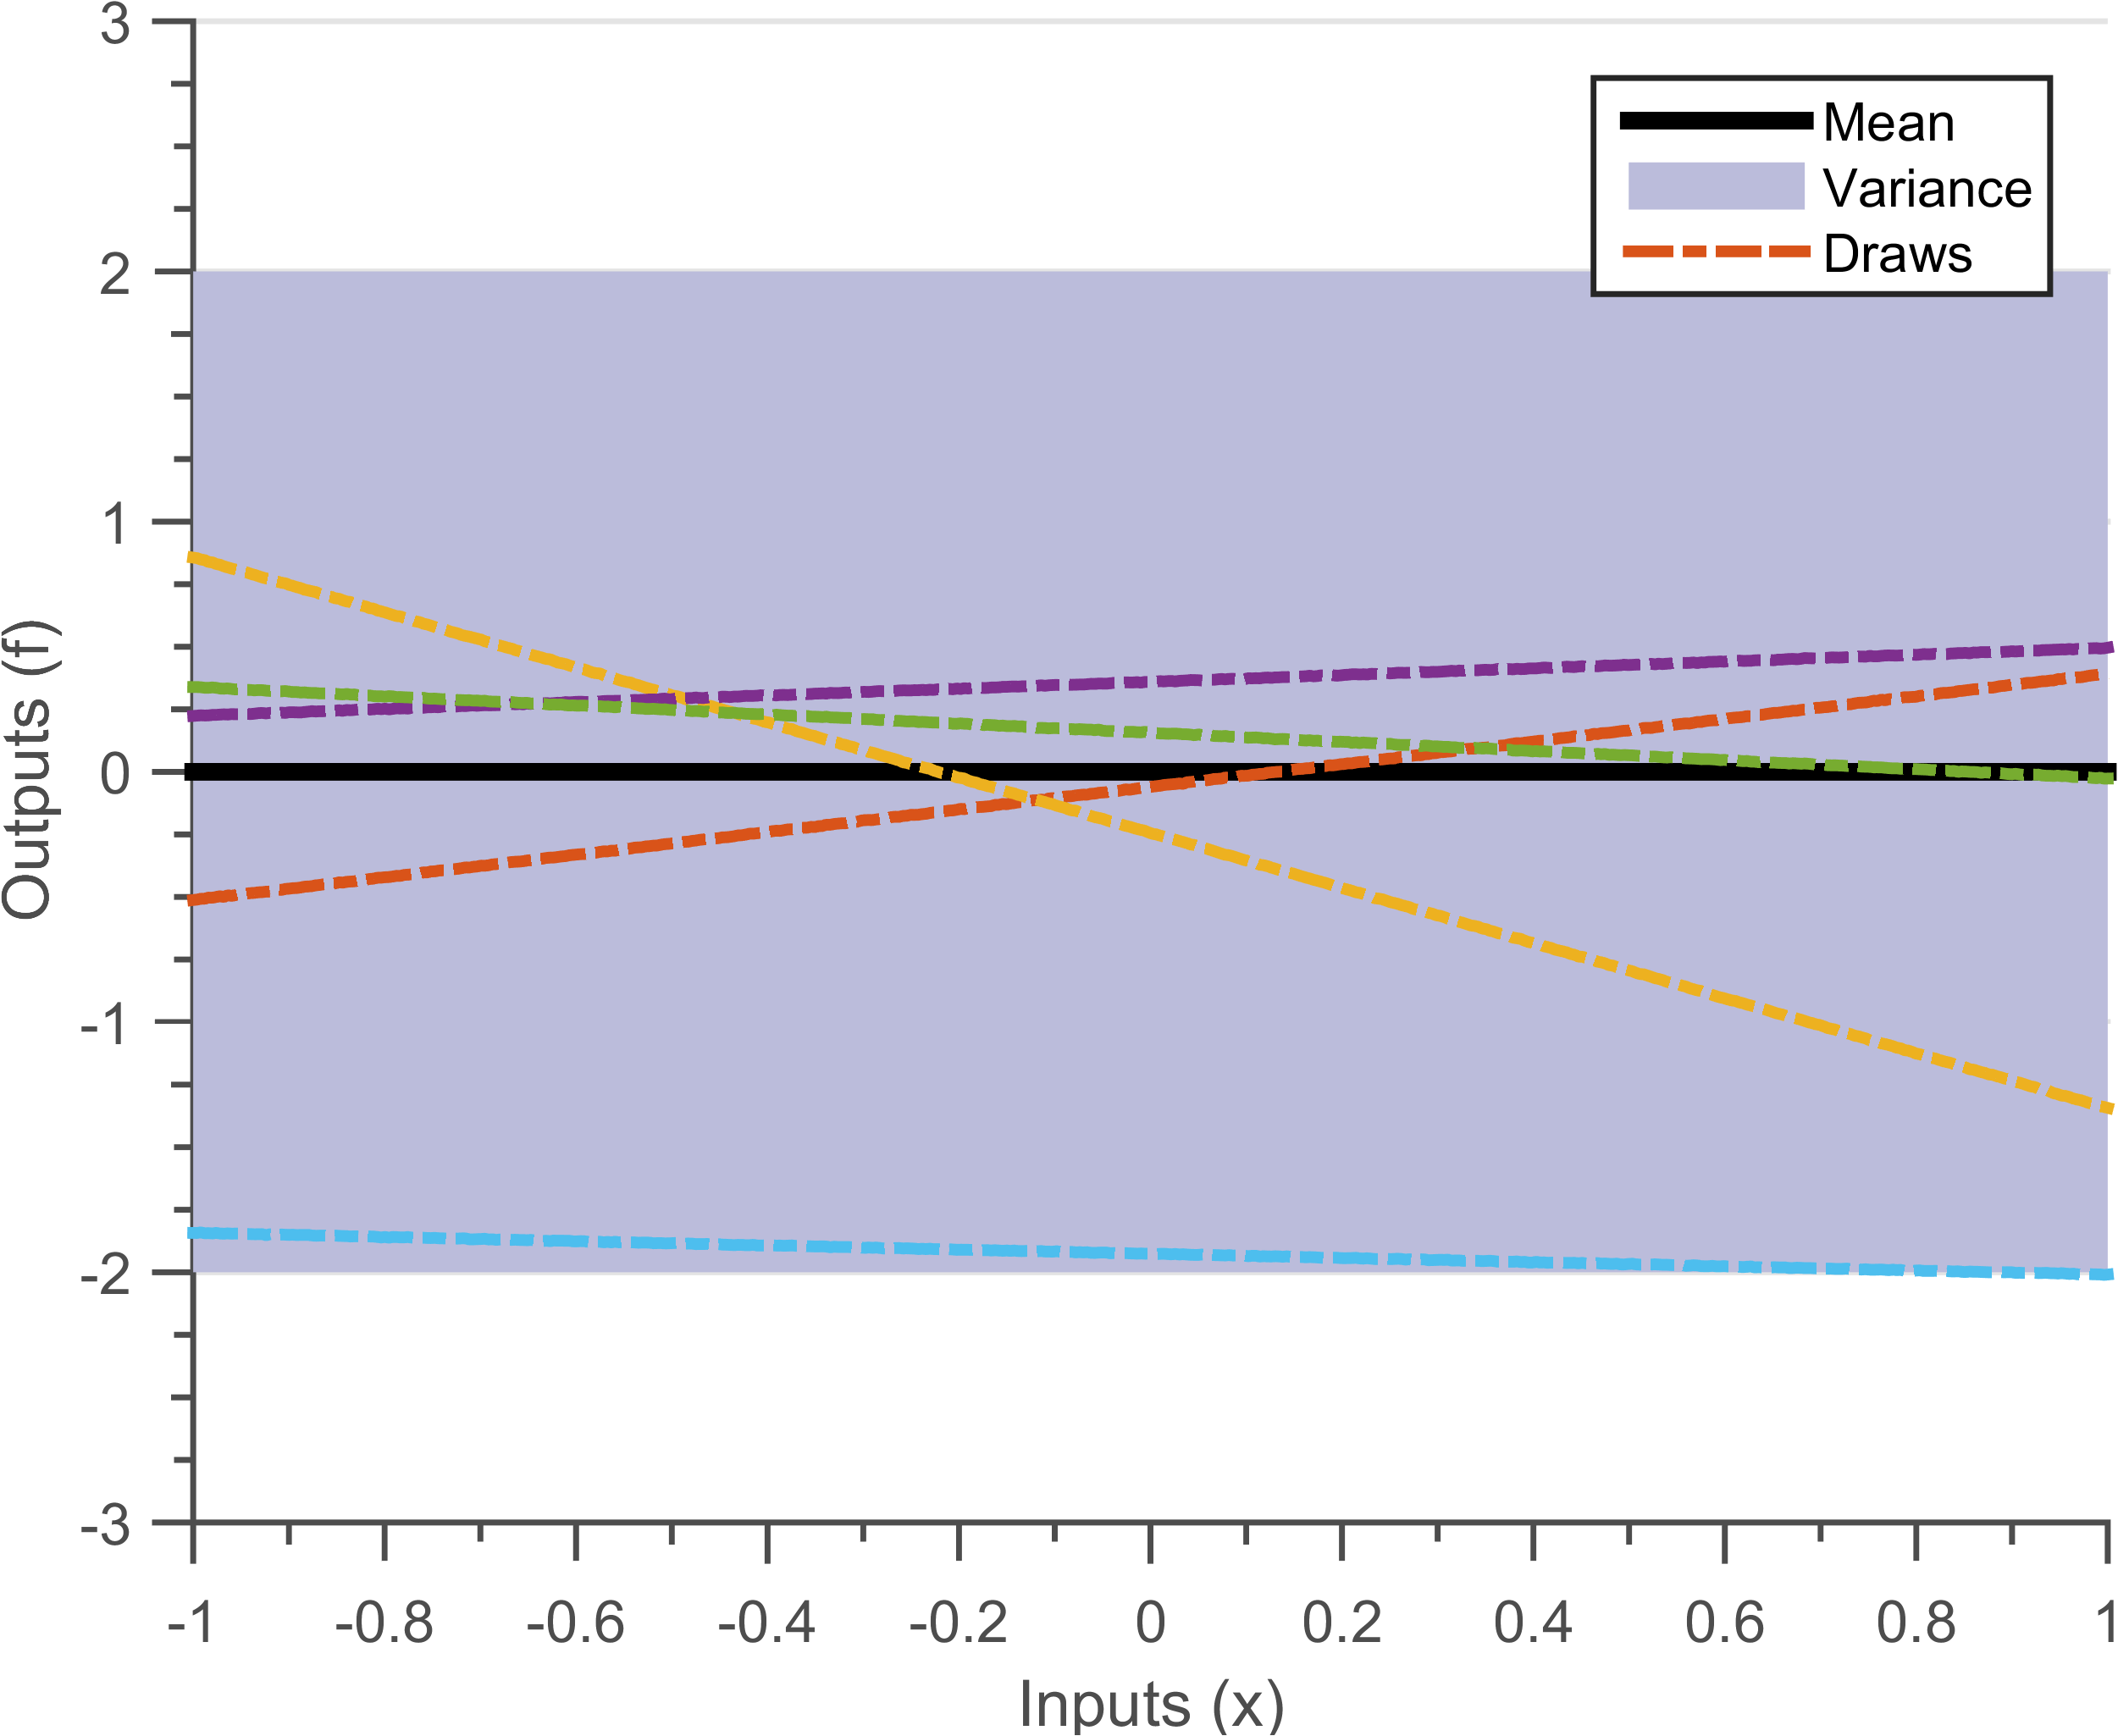
\includegraphics[width=0.45\textwidth]
        {images/part2/drawsLinear}
        \label{subFigdrawsLinear}
  }\quad
\subfigure[{Draws from a GP posterior with mean zero and Linear kernel (figure \ref{subFigdrawsLinear}) conditioned on the data $x = -0.5, y = 0$. The posterior mean passes from the data point, random functions drawn from a linear GP are linear}]
  {
        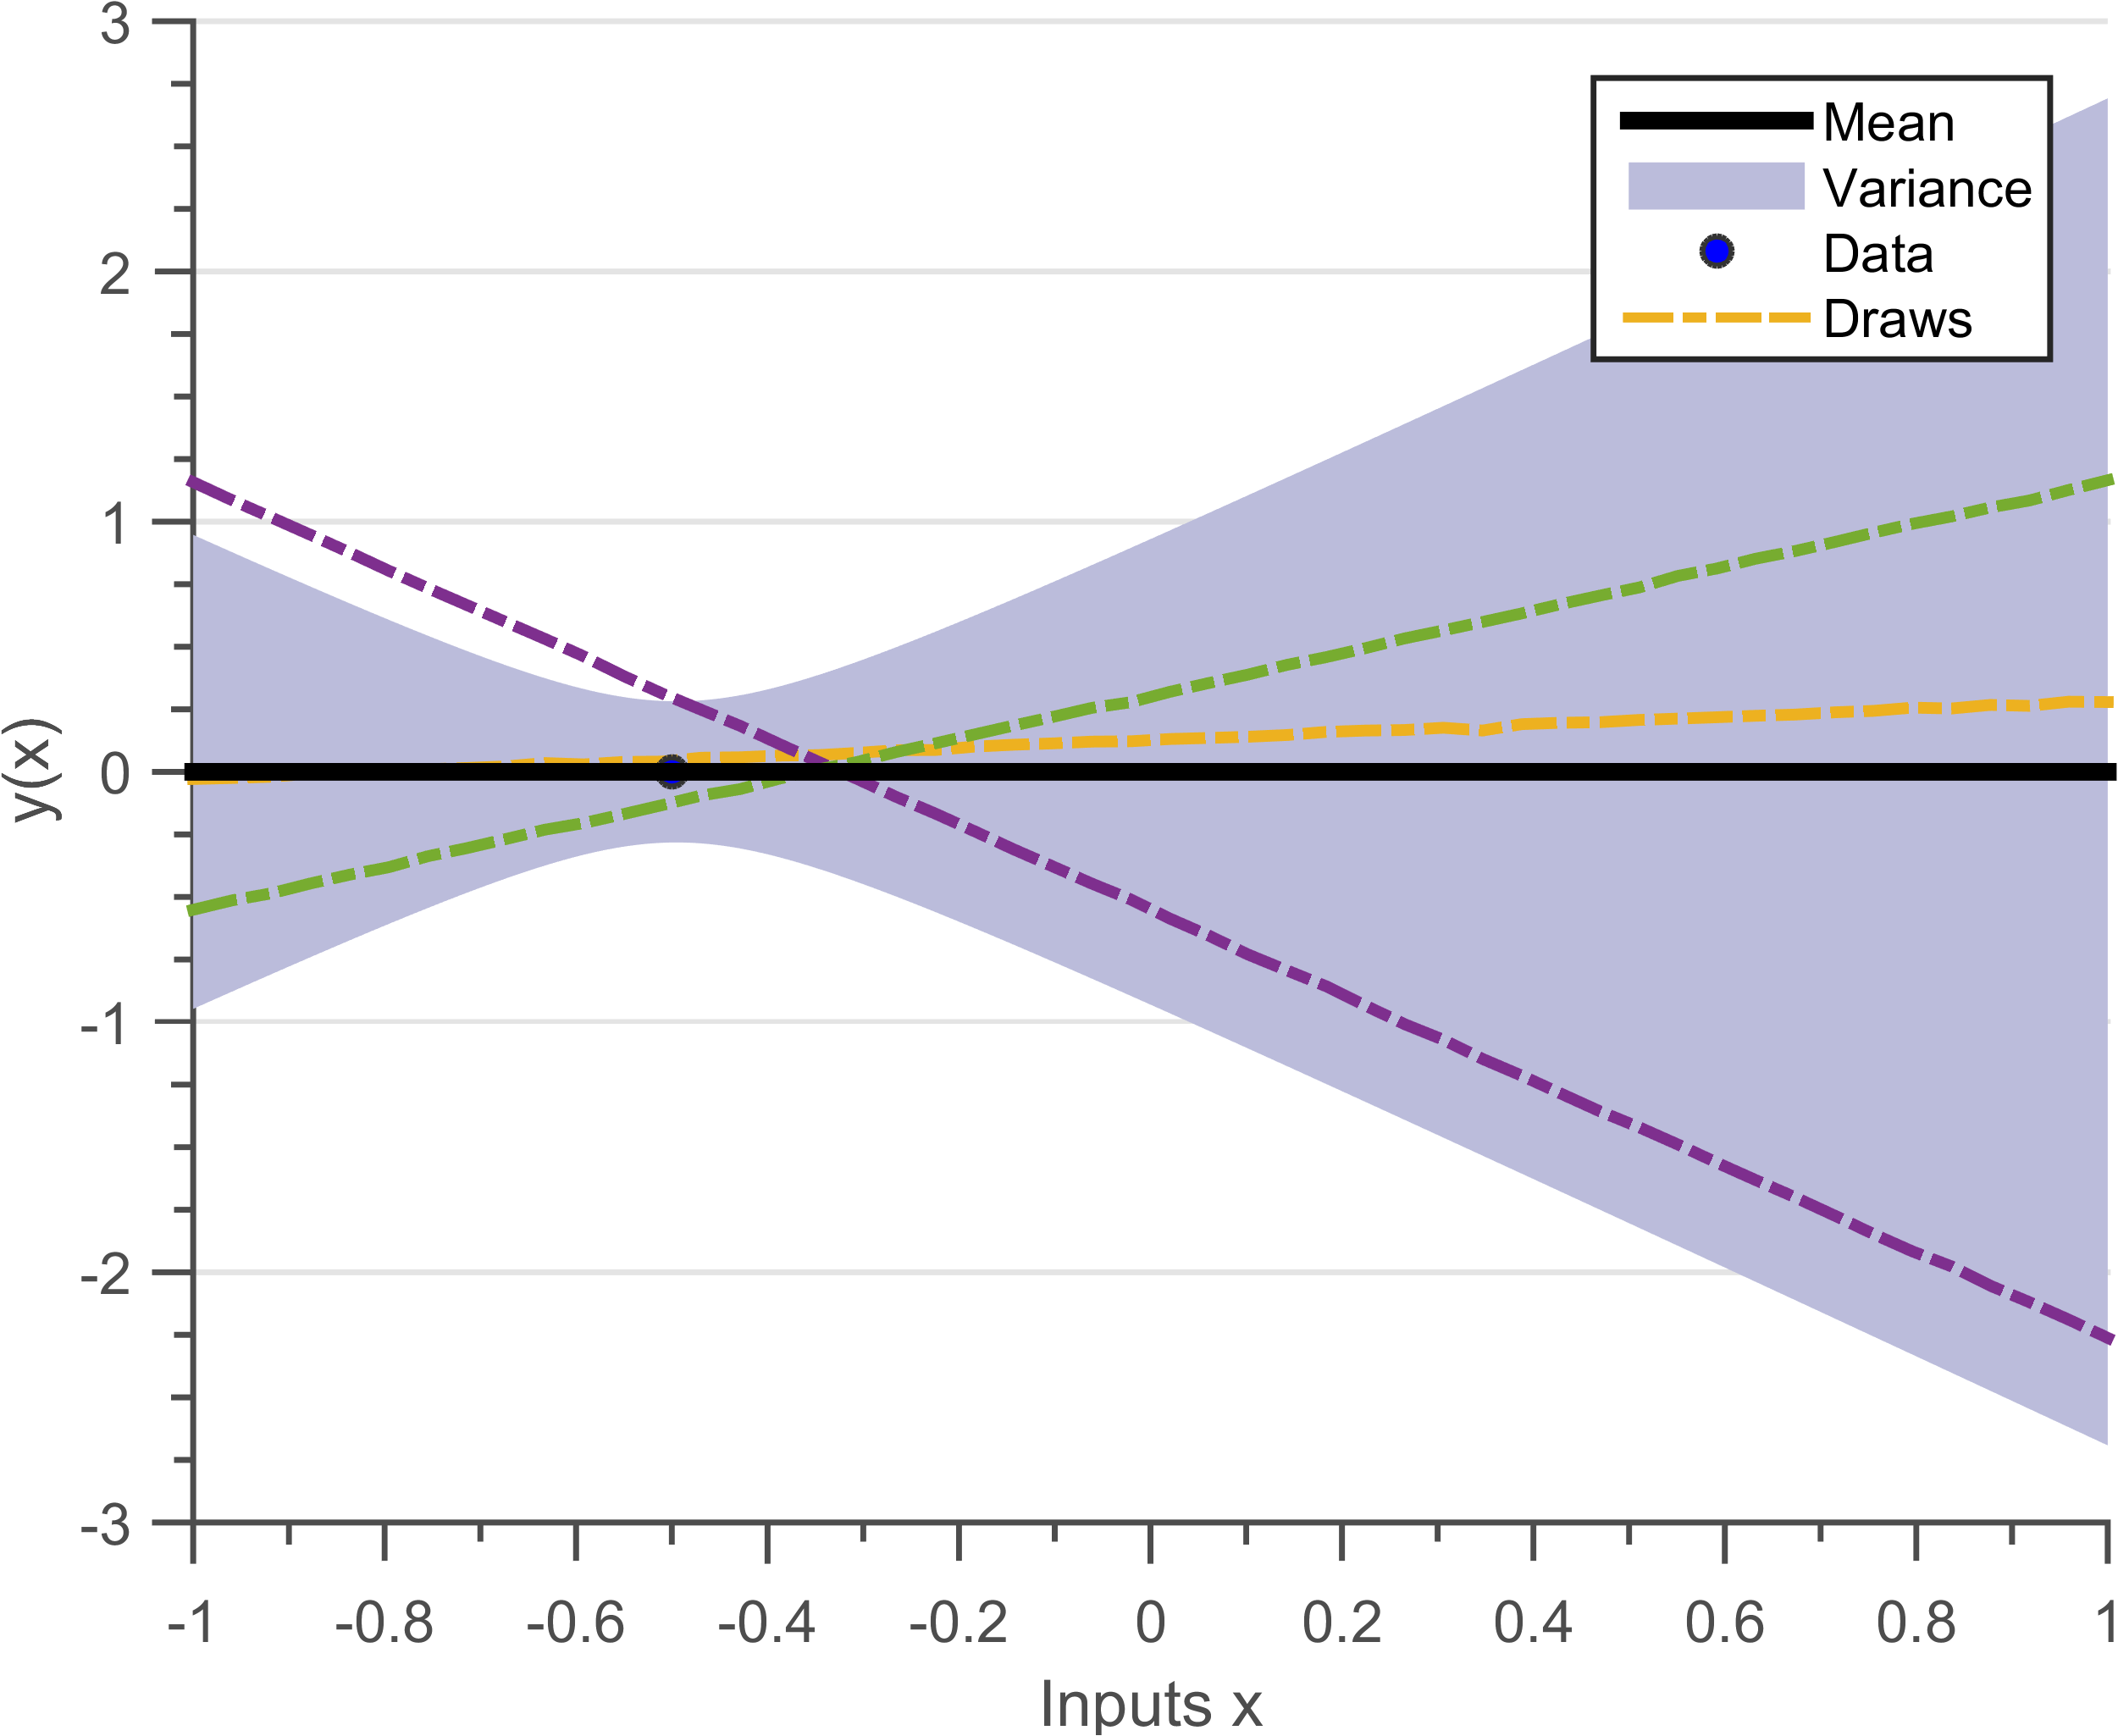
\includegraphics[width=0.45\textwidth]
        {images/part2/posteriorLinearNoisy_1}
        \label{subFigposteriorLinearNoisy_1}
  }\quad

       \caption{Prior and posterior from a GP prior of linear kernel. The solid black line defines the mean function, shaded blue region defines 95\% confidence interval (2$\sigma$) distance away from the mean. The dashed lines represent five functions drawn at random from a GP prior.}
       \label{figPriorAndPosteriorLinearKernel}
\end{figure}

\begin{mdframed}[hidealllines=true,backgroundcolor=lightgray!20]
Figure \ref{subFigmaximizingMarginalLikelihoodLinear} shows the contours of marginal likelihood with respect to intercept ($w_{0}$) and slope ($w_{1}$). The marginal likelihood is maximum for $w_{0} = 0.2576, w_{1} = 0.4584$, this same as posterior mean predicted in equation \ref{eqExperimentalPosterior}. This means that the data $\mathcal{D}_{1}$ has the highest possibility of coming from a data-set defined by a prior having these hyper-parameters. Figure \ref{subFigoptimizedPosteriorLinearNoisy_3} shows the posterior for same data set but for the hyper-parameters where marginal likelihood is maximum.
\end{mdframed}


\begin{figure}[!ht]
  \centering
    \subfigure[{Marginal likelihood contours for varying bias and slope parameter. The noise hyper-parameter is $(\sigma_{1} = [0.1])$. Marginal likelihood is maximum for $w_{0} = 0.2576, w_{1} = 0.4584$.}]
  {
        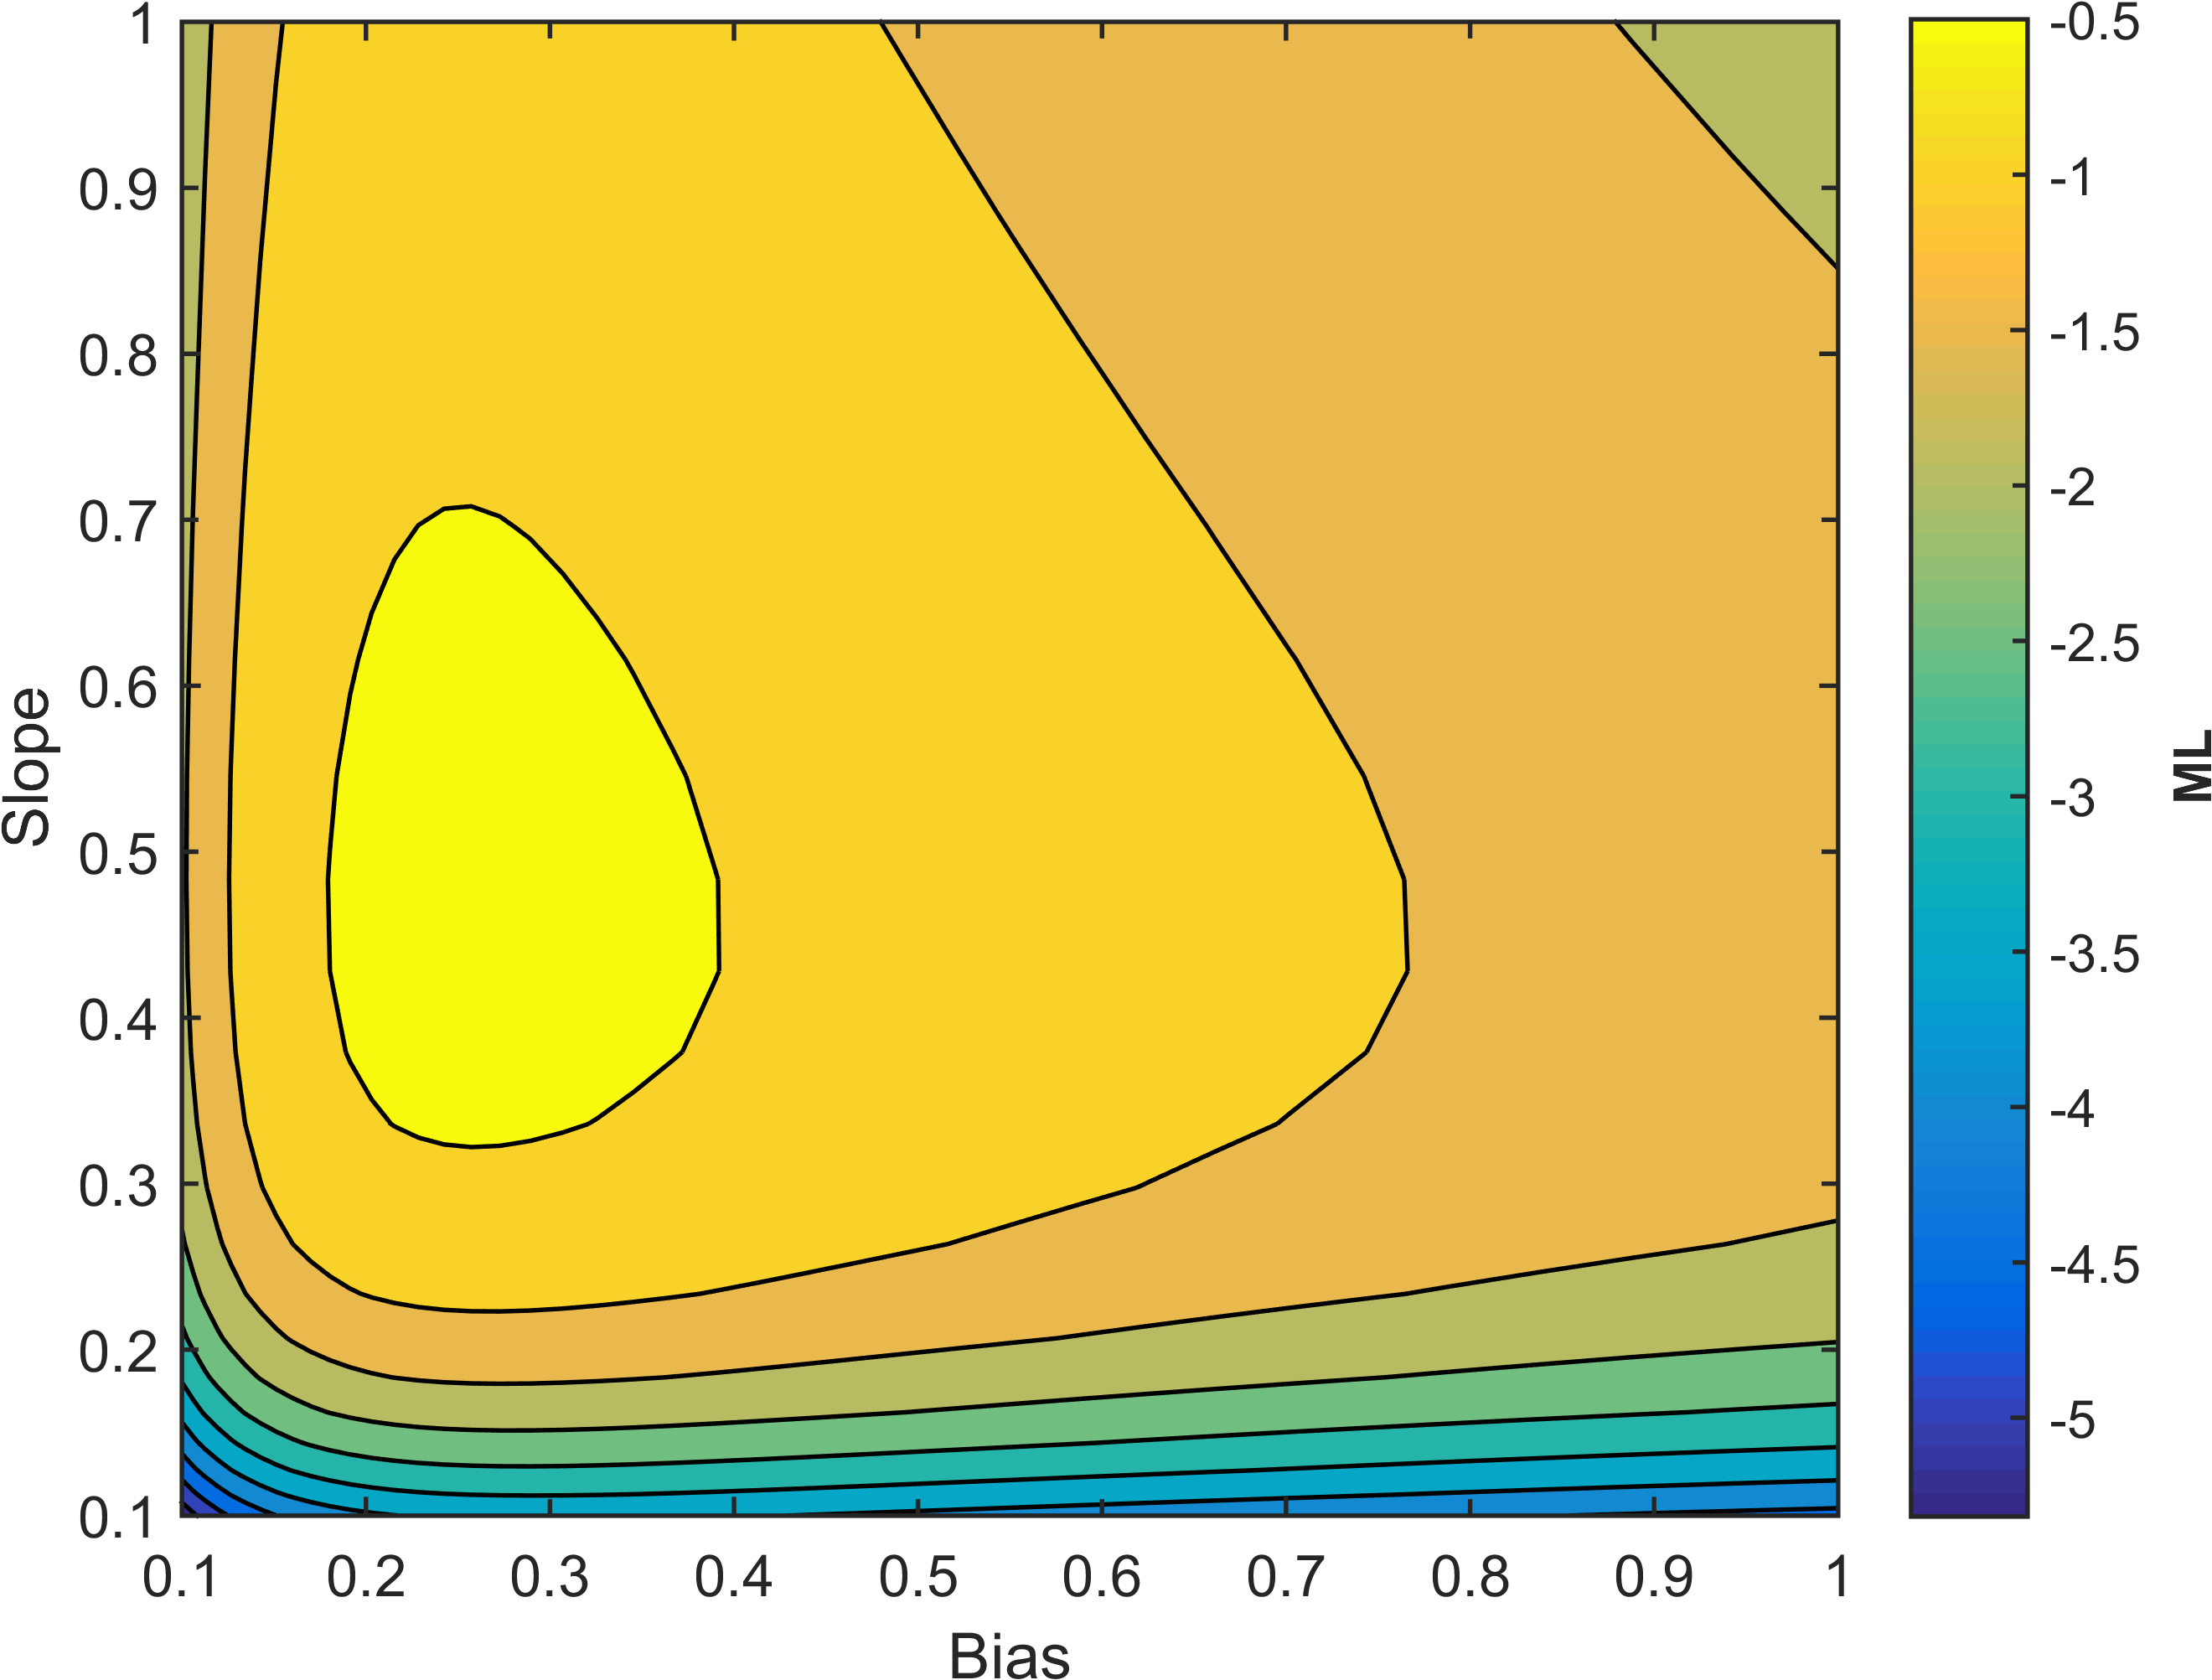
\includegraphics[width=0.45\textwidth]
        {images/part2/maximizingMarginalLikelihoodLinear}
        \label{subFigmaximizingMarginalLikelihoodLinear}
  }\quad
\subfigure[{Draws from a GP posterior, conditioned on the data-set $\mathcal{D}_{1}$ with mean zero and Linear kernel with hyper-parameters that maximize the marginal likelihood.}]
  {
        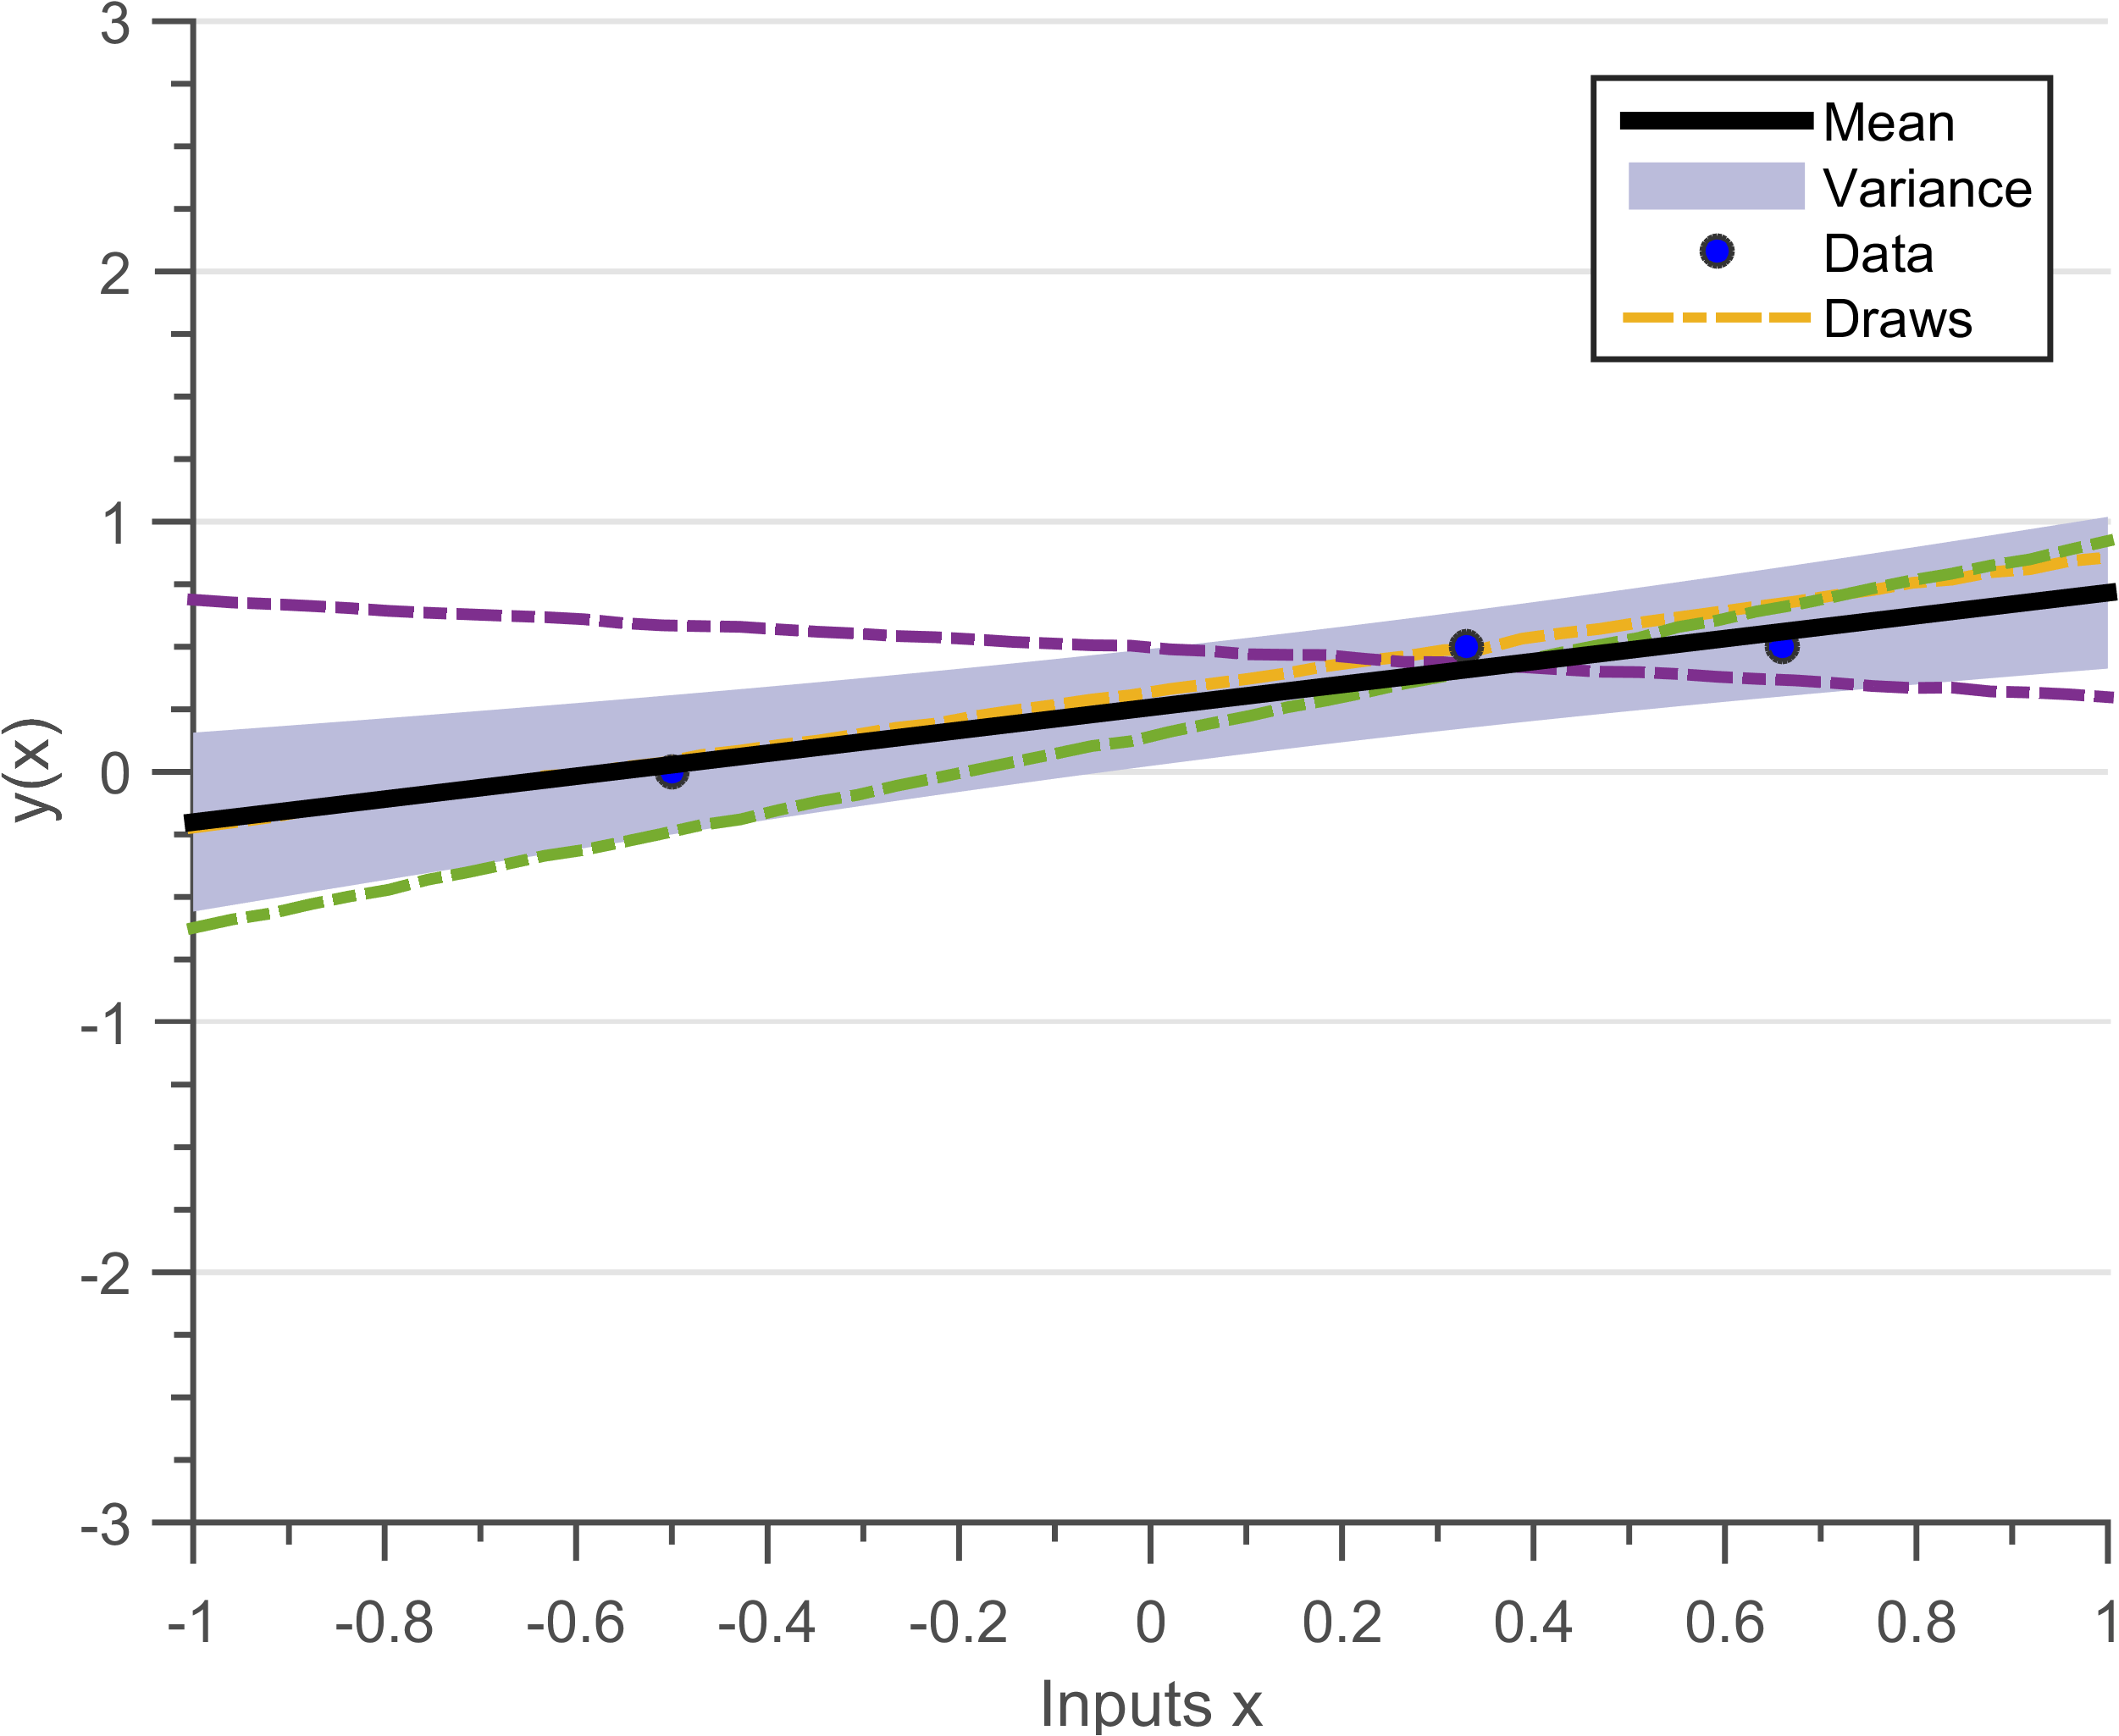
\includegraphics[width=0.45\textwidth]
        {images/part2/posteriorLinearNoisy_3}
        \label{subFigoptimizedPosteriorLinearNoisy_3}
  }\quad

       \caption{Maximizing Marginal Likelihood Linear kernel}
       \label{figMaximizingMLLinearKernel}
\end{figure}

\subsection{Neural Network Kernel}\label{subSecCh4NNkernel}
It can be shown that a neural network with infinitely many hidden units and an error activation function ($erf(z)$) tends to a GP with a Neural network kernel \cite{neal2012bayesian} (equation \ref{eqnNNKernel}). 

\begin{equation}\label{eqnNNKernel}
K_{NN}(x_{1}, x_{2}, \theta) = \theta_{1}^{2}\frac{2}{\pi} sin^{-1}\left ( \frac{2 x_1 \theta_{2} x_2}{\sqrt{(1+2 x_{1}^{T}\theta_{2} x_1)(1+2x_{2}^{T}\theta_{2}x_{2})}} \right )
\end{equation}

\marginnote{\textsl{Hyper-parameters}}[1cm]
The hyper-parameters $(\theta = [\theta_{1}, \theta_{2}])$ are; amplitude $\theta_{1}$ which defines average distance from mean and the length scale $\theta_{2}$ which define the smoothness of functions. GPs with this covariance function define a space of superimposed sigmoidal functions. Figure \ref{figNNPrior} shows random draws from a Neural Network kernel but with varying value of hyper-parameters. Figure \ref{subfig:drawsNN100} has a higher value of smoothness hyper-parameter ($\theta_{2}$) than figure \ref{subfig:drawsNN10}, which makes the constituent functions have stronger slope. Hence, we can use this kernel to approximate the presence of discontinuity in our family of functions. 

\begin{figure*}[!ht]
  \centering
  \subfigure[{Draws from a GP prior with mean zero and Neural Network kernel (equation \ref{eqnNNKernel}) with $\theta = [1, 10]$.}]
  {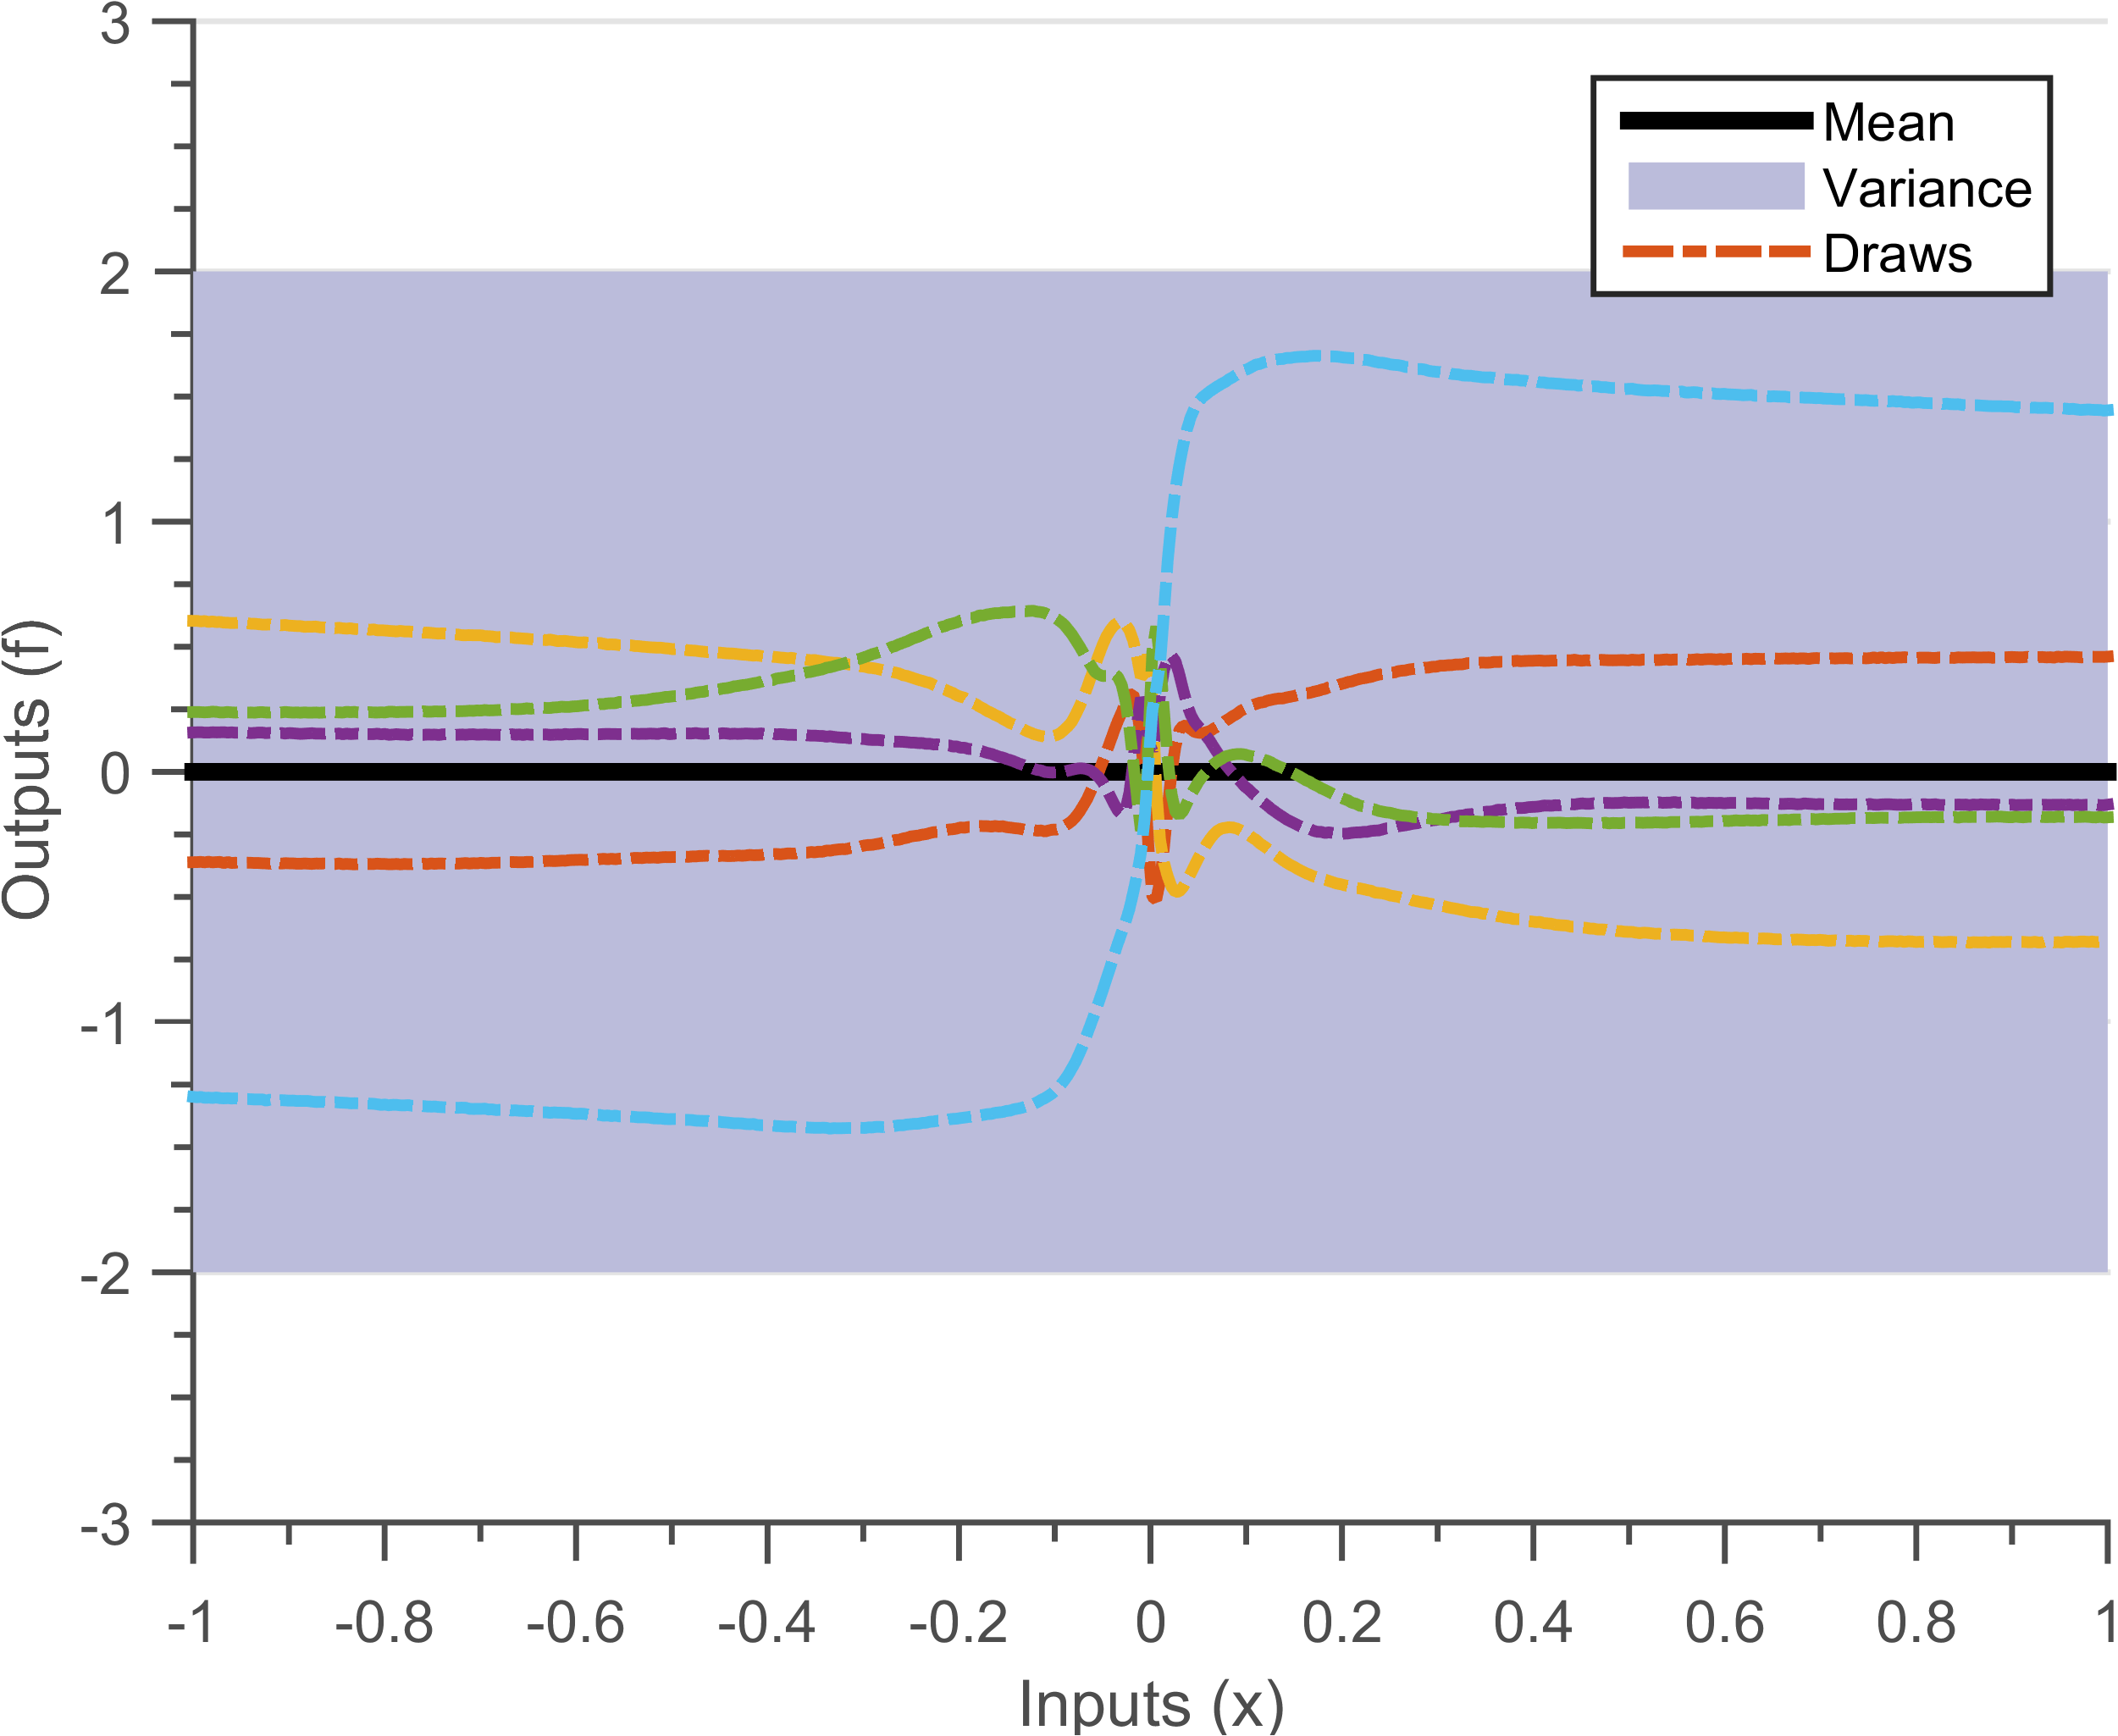
\includegraphics[width=0.45\textwidth]{images/part2/drawsNN10}\label{subfig:drawsNN10}}\quad
    \subfigure[{Draws from a GP prior with mean zero and Neural Network kernel (equation \ref{eqnNNKernel}) with $\theta = [1, 100]$. Higher value of $\theta_{2}$ signifies increasing slope}]
  {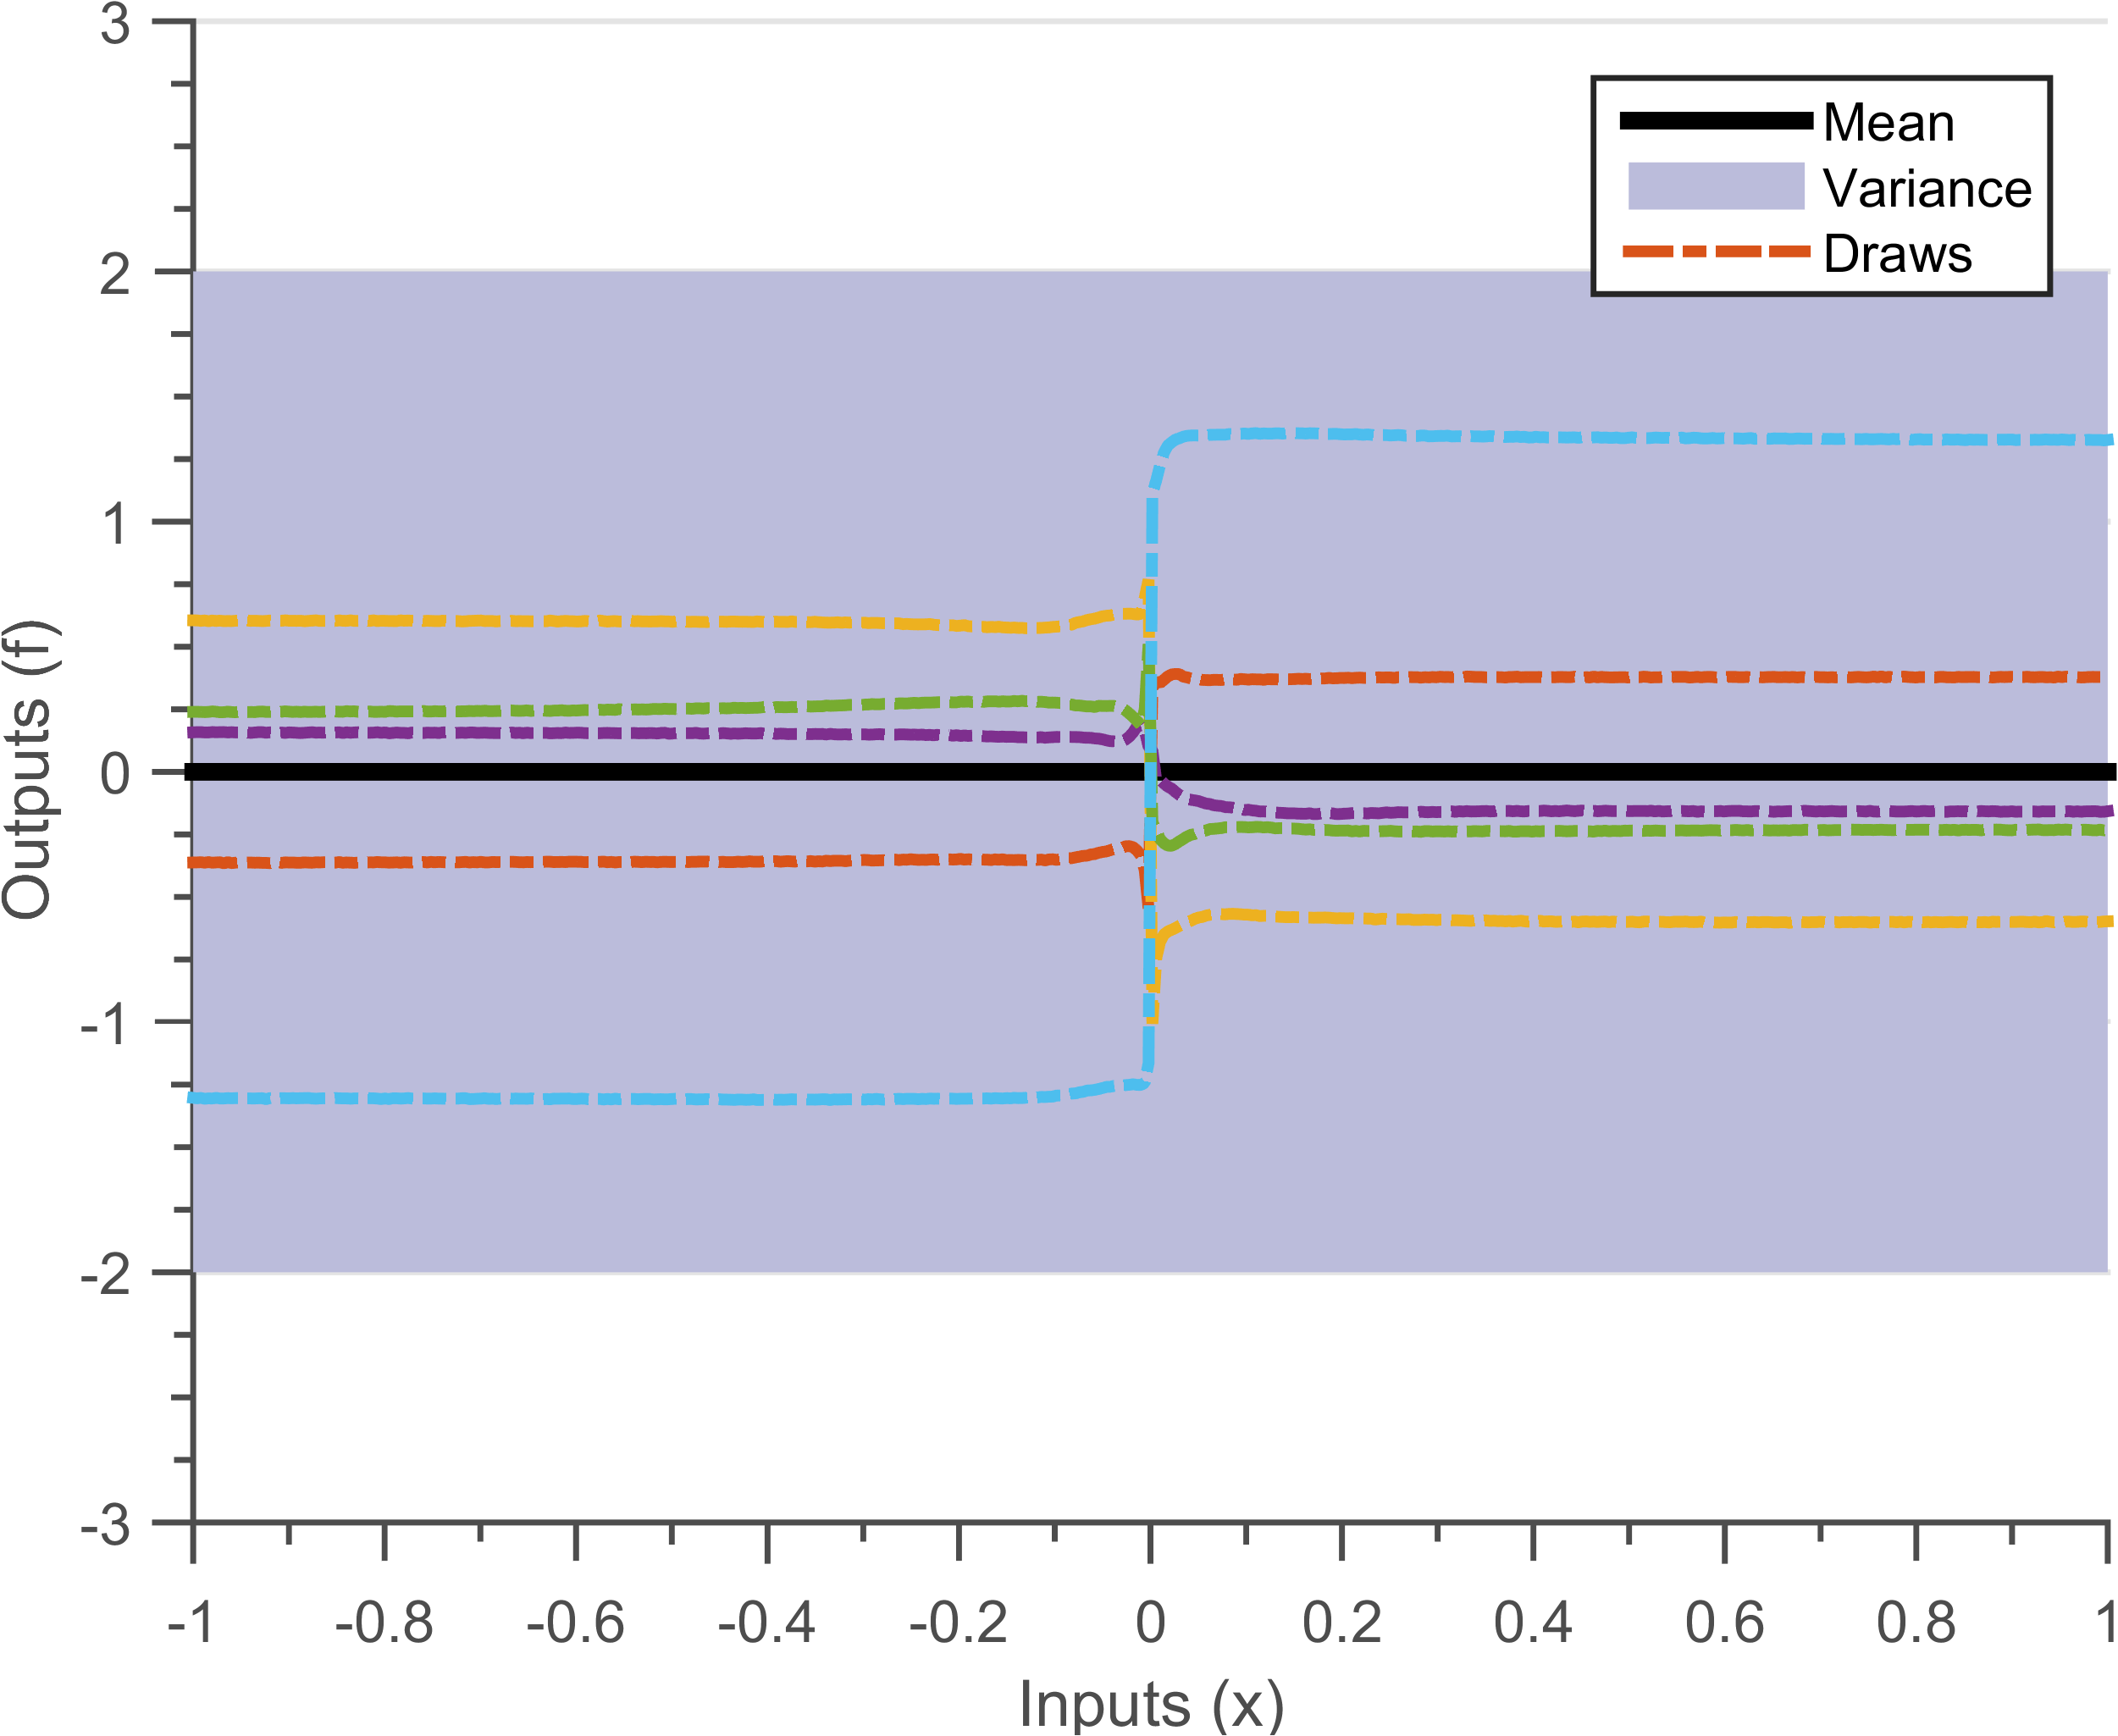
\includegraphics[width=0.45\textwidth]{images/part2/drawsNN100}\label{subfig:drawsNN100}}\quad
  \caption{Draws from Neural Network kernels having different hyper-parameters. The solid black line defines the mean function, shaded blue region defines 95\% confidence interval (2$\sigma$) distance away from the mean. The dashed lines represent five functions drawn at random from a GP prior.}
  \label{figNNPrior}
\end{figure*}

\subsection{Constant and Noise kernel}
A constant covariance function (equation \ref{eqConstantKernel}) defines a constant function. Here, $\sigma_{constant}$ defines the possible amplitude of the constant function.

\begin{align}
k_{constant} & = \sigma^2_{constant} \label{eqConstantKernel} \\
k_{noise}(x_{1}, x_{2}) & = \sigma^2_{noise}\delta_{x_{1}x_{2}} \label{eqNoiseKernel}
\end{align}

On the other hand, equation \ref{eqNoiseKernel} defines a white noise kernel, the $\sigma_{noise}$ defines the amplitude of noise. $\delta_{x_{1}x_{2}}$ is a Kronecker delta function which is $1$ if $x_{1} = x_{2}$ and zero otherwise, this means that observations at two inputs are independent of each other. 

\section{Stationary kernels} \label{secStationaryKernels}
Covariance functions which are purely a function of distance $d = (x_{1} - x_{2})$ are called as stationary functions, Whereas covariance functions which are functions of absolute value of distance $d = |x_{1} - x_{2}|$ are called as isotropic covariance functions. Stationary covariance functions remain unchanged if the points $x_{1}, x_{2}$ are translated. Hence a family of functions defined by stationary kernels will have similar local features throughout the input domain. 

\marginnote{\textsl{\textit{Bochner's theorem}}}[1cm]
The \textit{Bochner's theorem} defines a relationship between a stationary covariance function and its Fourier transform. It states that the Fourier transform of a stationary covariance function exists and is a positive finite measure. If $k(d)$ is a stationary covariance function (equation \ref{eqCh4StationaryCovariance}) then $S(s)$ is its Fourier transform (equation \ref{eqCh4StationaryPowerSpectrum}), also called the power spectrum or spectral density \cite{bochner1959lectures, Stein1999Springer, cox1977theory}. A positive finite measure in this context means that $S(s)$ is non-negative for all frequencies $s$, and integral in equation \ref{eqCh4StationaryCovariance} is finite.

\begin{equation}\label{eqCh4StationaryCovariance}
    k(d) = \int S(s) e^{2 \pi is^{T} d}ds
\end{equation}

\begin{equation}\label{eqCh4StationaryPowerSpectrum}
    S(s) = \int k(d) e^{-2 \pi is^{T} s}dd 
\end{equation}

\marginnote{\textsl{Power spectrum}}[1cm]
The power spectrum is a more interpretable method of understanding constituent functions in a hypothesis space. A covariance function probabilistically defines a hypothesis space, the power spectrum corresponding to this covariance function tells us the power of the frequencies in this hypothesis space. If a power spectrum has more power at lower frequencies, then the constituent functions in its hypothesis space will be more smooth. Whereas, if the power spectrum has more power at higher frequencies, then the constituent functions in its hypothesis space will be less smooth \cite{wilson2014thesis}. 

\subsection{Squared Exponential Kernel}\label{subSecCh4SEKernel}
We have already encountered the SE kernel in section \ref{subSecCH2Covariance}. It is one of the most widely used kernel because it defines a hypothesis space of infinitely differentiable (infinitely smooth) functions. The SE kernel is Gaussian in shape (equation \ref{eqnKSESquaredExponential}), which makes its Fourier transform also Gaussian in shape (equation \ref{eqnSSESquaredExponential}).  

\begin{equation}\label{eqnKSESquaredExponential}
k_{SE}(d, \theta) = \theta_{amplitude}^2exp \left [-\frac{d^2}{2\theta_{lengthScale}^2} \right ]
\end{equation}

\begin{equation}\label{eqnSSESquaredExponential}
S_{SE}(s, \theta) = \theta_{amplitude}^2  exp \left [-2\pi \theta_{lengthScale}^2 s^2 \right]
\end{equation}

\marginnote{\textsl{Hyper-parameters}}[1cm]
The two hyper-parameters of the SE kernel are the amplitude hyper-parameter ($\theta_{amplitude}$), which defines the amplitude of functions and the length-scale hyper-parameter ($\theta_{lengthScale}$), which defines the smoothness of functions. Figure \ref{subFigkernelFunctions} plots the covariance values of SE kernel with hyper-parameters $\theta_{amplitude}=1$ and $\theta_{lengthScale}=1$, for varying values of $d$ whereas figure \ref{subFigspectralFunctions} plots the power spectrum for SE kernel for the same hyper-parameters . 

\marginnote{\textsl{Interpretation}}[1cm]
As discussed earlier, the covariance function ($k_{SE}$) defines the measure of similarity between two input points, if two points have high value of covariance then their output values ($y$) will be similar. If we increase $\theta_{lengthScale}$ then $k_{SE}$ will also increase, for the same value of $d$ and $\theta_{amplitude}$. This means that, the points for same value of $d$ will become more similar and hence the constituent functions in the hypothesis space will become more smooth. As length-scale increases the constituent functions tend to become smoother. Another way to interpret the effect of length-scale is by observing the power spectrum ($S_{SE}$). If we increase $\theta_{lengthScale}$ then $S_{SE}$ will start decreasing, for the same values of $s$ and $\theta_{amplitude}$. This means that less power will be allocated to higher frequencies and hence the constituent functions in the hypothesis space will become more smooth (Figure \ref{figGPPriors}). 

Figure \ref{subFigkernelFunctionsSE} plots the covariance values of SE kernel (($\theta_{amplitude} = 1$) for various values of length-scales ($\theta_{lengthScale} = [0.1, 1, 100]$)) whereas figure \ref{subFigspectralFunctionsSE} plots the power spectrum for same kernels. We can see that the power spectrum ($S(s)$) for lower length-scales has less power at higher frequencies, meaning that their corresponding hypothesis spaces will not have faster moving functions. 

\begin{figure}[!ht]
  \centering
    \subfigure[{Kernel density for SE kernel with three different length-scales. The hyper-parameters are amplitude ($\theta_{amplitude} = 1$) and length-scale ($\theta_{lengthScale} = [0.1, 1, 100]$). $k(d)$ for $\theta_{lengthScale} = 100$ resembles a constant function.} ]
  {
        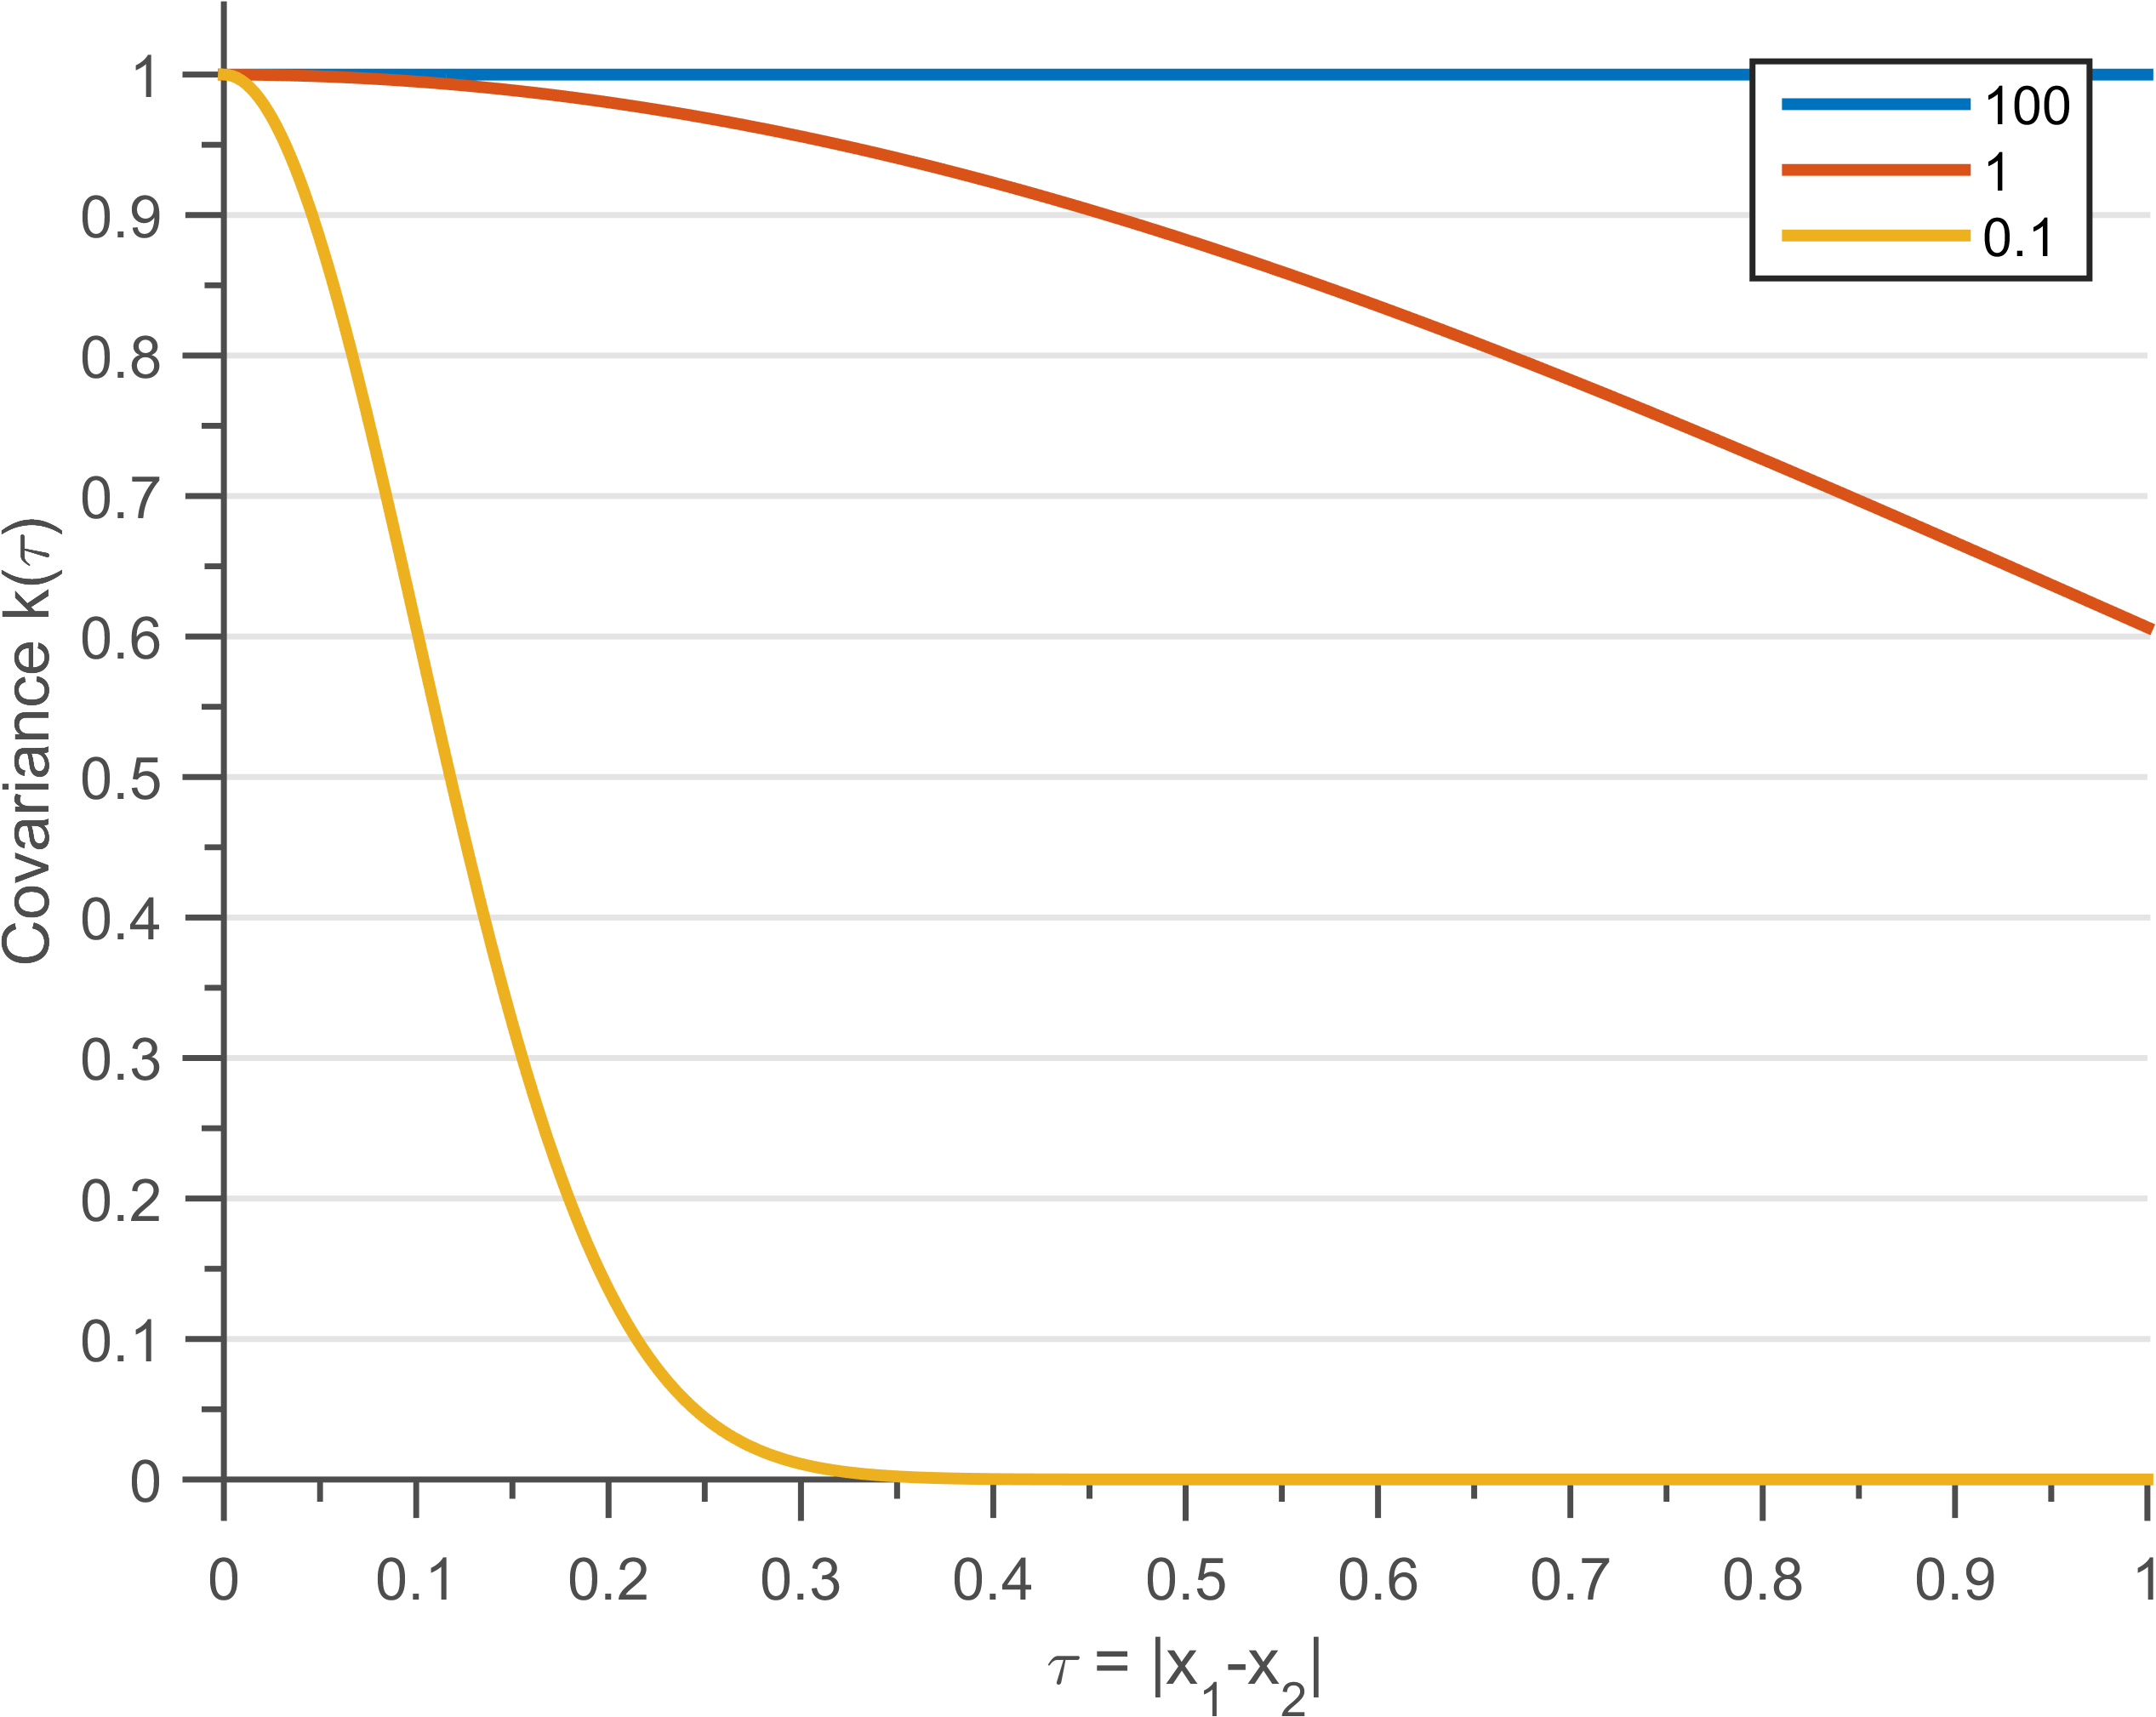
\includegraphics[width=0.45\textwidth]
        {images/part2/kernelFunctionsSE}
        \label{subFigkernelFunctionsSE}
  }\quad
\subfigure[{Power spectrum for SE kernel with three different length-scales. The hyper-parameters are amplitude ($\theta_{amplitude} = 1$) and length-scale ($\theta_{lengthScale} = [0.1, 1, 100]$). $S(s)$ for $\theta_{lengthScale} = 0.1$ resembles a constant function, while for $\theta_{lengthScale} = 100$ $S(s)$ resembles a dirac-delta function.}]
  {
        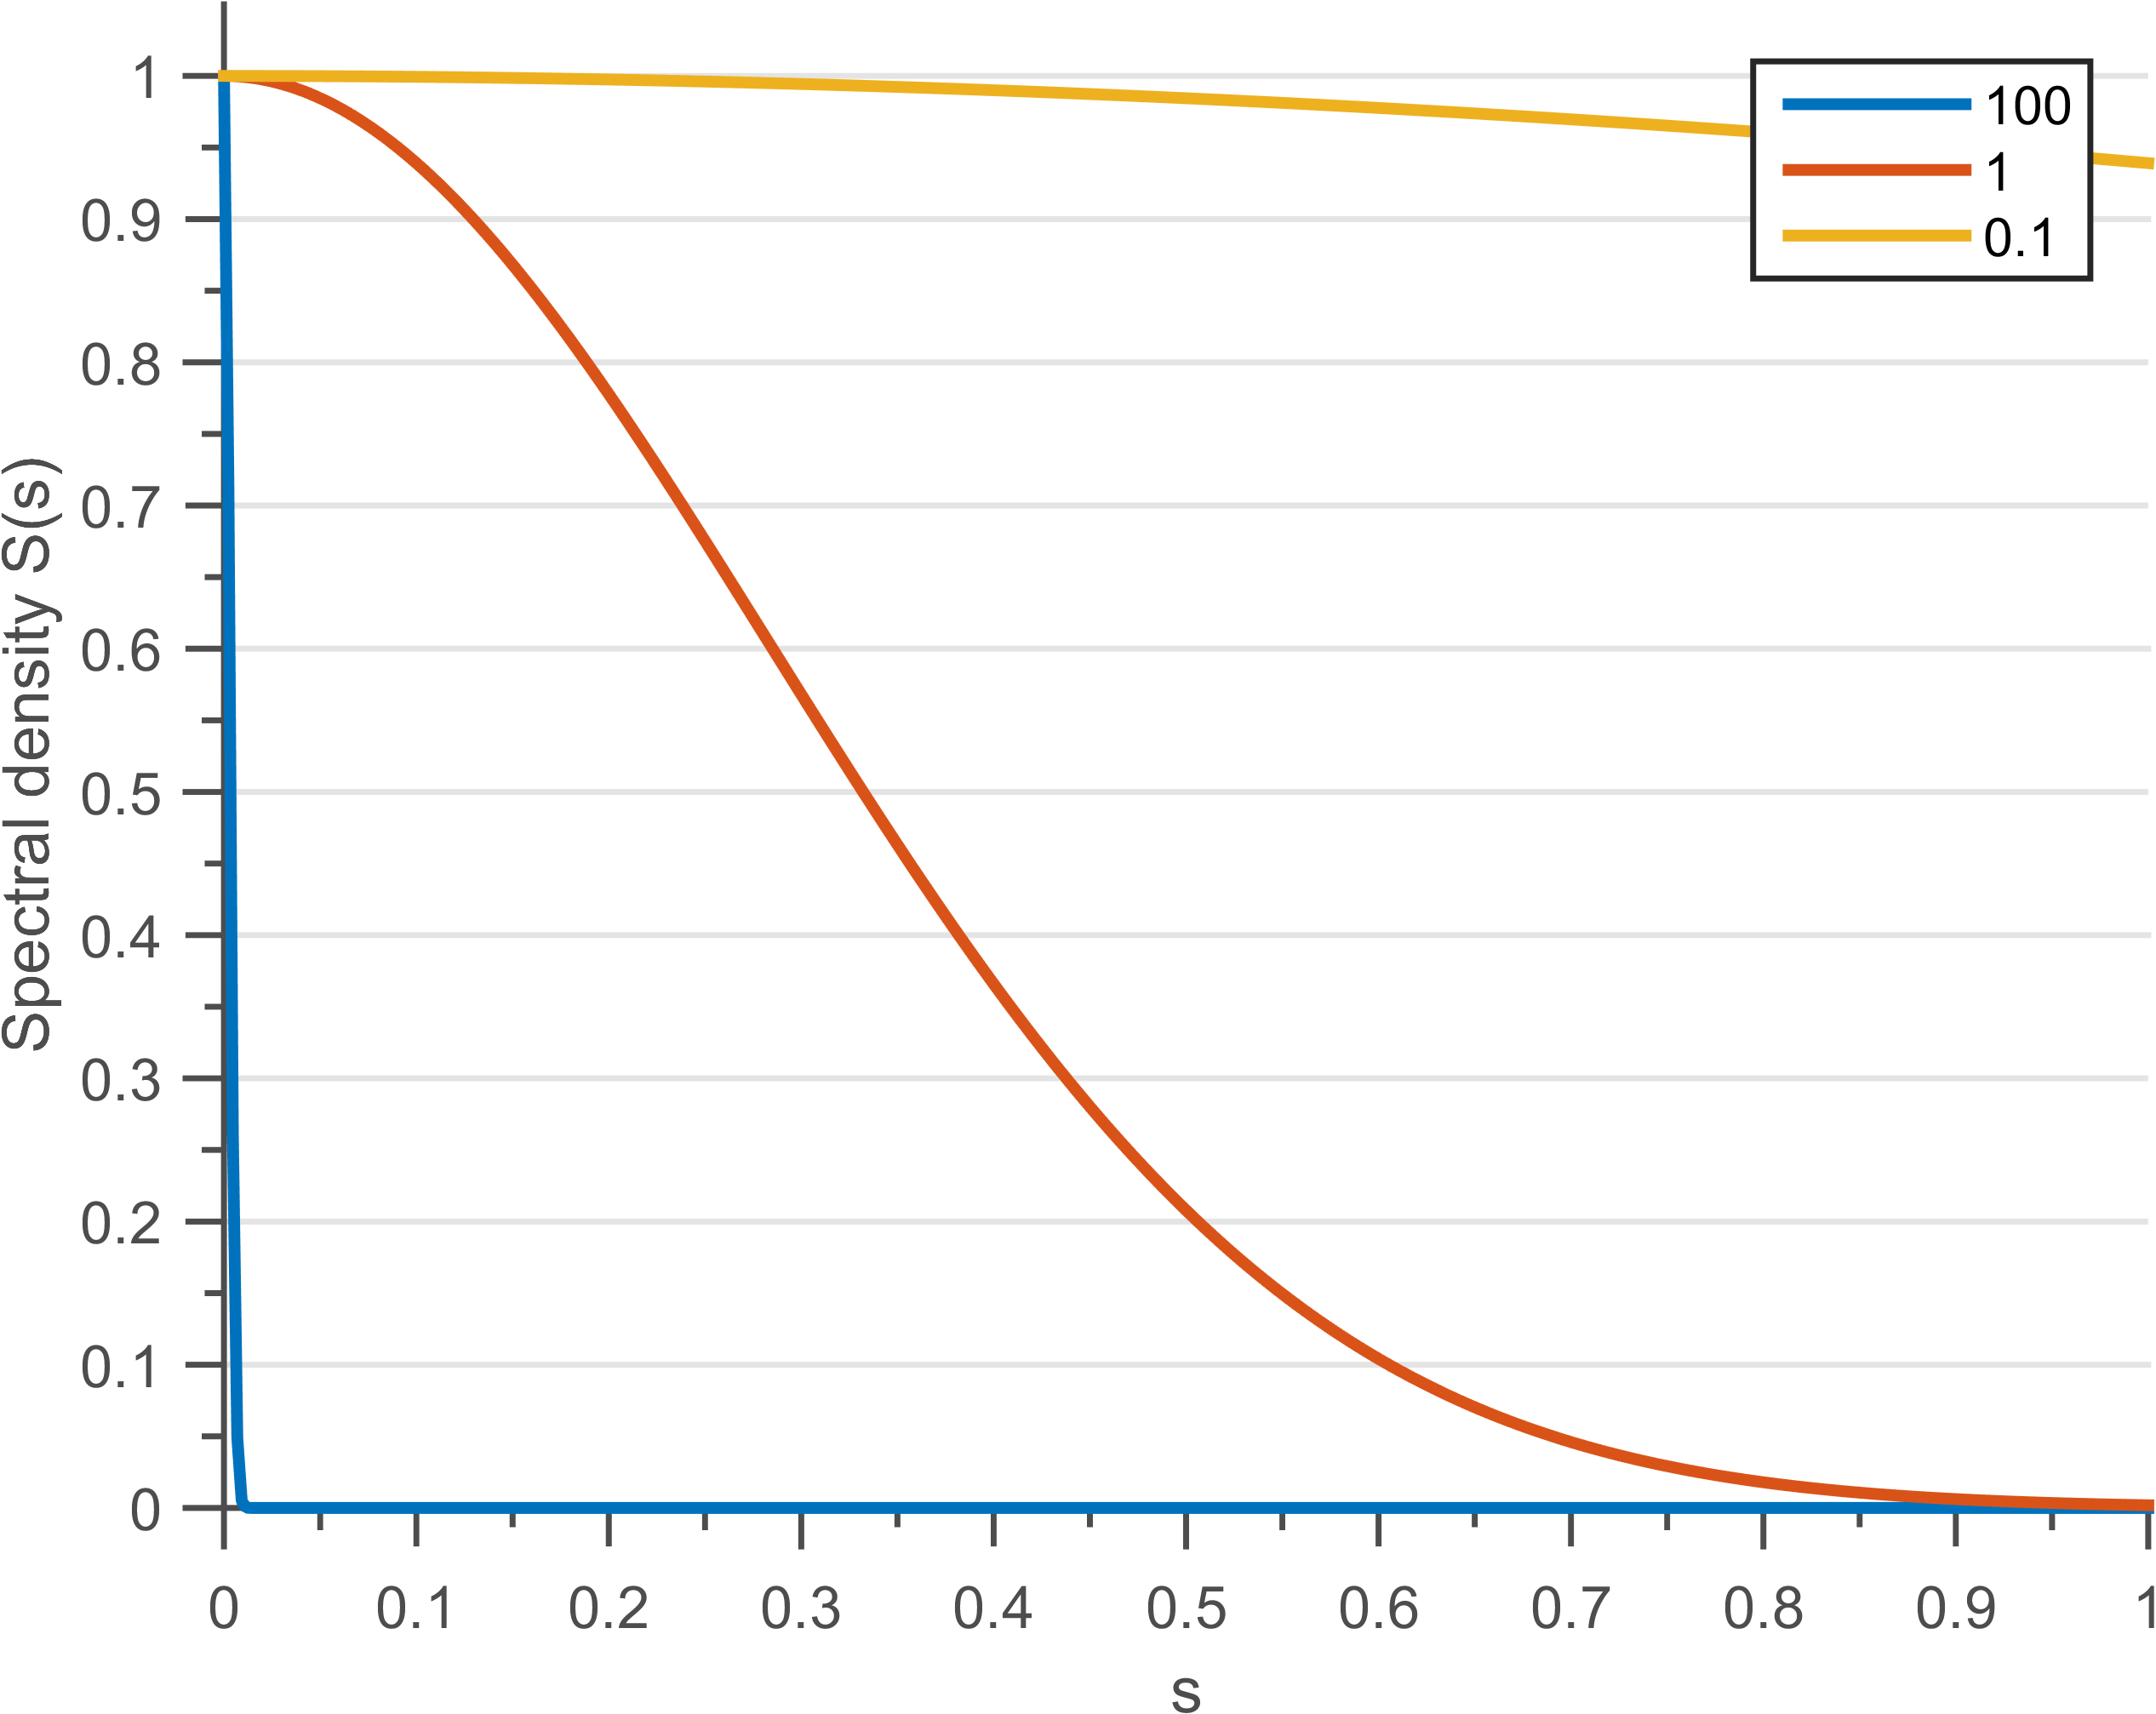
\includegraphics[width=0.45\textwidth]
        {images/part2/spectralFunctionsSE}
        \label{subFigspectralFunctionsSE}
  }\quad
\caption{Covariance functions and Power spectrums for SE kernel with three different length-scales}
       \label{figKernelAndPowerSpectrumsSE}
\end{figure}

Note, as $\theta_{lengthScale}$ tends to infinity, an SE kernel tends to a constant covariance function (Fourier transform of a constant function is a delta function). Whereas, if $\theta_{lengthScale}$ tends to zero, an SE kernel tends to a white noise kernel (Fourier transform of a delta function is a constant function).

\subsection{Mat\'ern Kernel}\label{subsecCh4MaternKernel}
The Mat\'ern kernel is the second most popular kernel after the squared exponential. This kernel is derived using a t-distribution as the power spectrum ($S(s)$) and calculating its inverse Fourier transform. A t-distribution has more weight on higher-frequencies (when compared to a Gaussian distribution) and hence gives rise to more non-smooth functions. 

\begin{equation}
k_{Matern}(\nu, d, \theta) = \theta_{amplitude}^2\frac{2^{1- \nu }}{\Gamma (\nu)}\left ( \frac{\sqrt{2\nu(d))}}{\theta_{lengthScale}} \right )^{\nu}K_{\nu}\left ( \frac{\sqrt{2\nu(d))}}{\theta_{lengthScale}} \right)
\end{equation}

\marginnote{\textsl{Differentiability}}[1cm]
$k_{Matern}$ is the covariance function for a Mat\'ern kernel, $\nu$ is a positive parameter which signifies the degrees of freedom in the t-distribution of the power spectrum. $\Gamma (\nu)$ is a Gamma function, while $K_{\nu}$ is a modified Bessel function. The Mat\'ern kernel provides the flexibility to define a hypothesis space of functions with varying degree of differentiability, due to this property they are often used to build machine learning models \cite{minasny2005matern, cornford2002modelling}. The degree of differentiability of the functions in the hypothesis space can be set as [$\nu-1/2$], i.e.  $\nu = 1/2$ (equation \ref{eqnExponential}) defines family of non-differentiable but continuous functions, $\nu = 3/2$ (equation \ref{eqnMAT32}) defines a family of functions differentiable only once and $\nu = 5/2$ (equation \ref{eqnMAT52}) defines a family of twice differentiable functions. Note, as $\nu$ tends to $\infty$ a t-distribution tends to a Gaussian distribution, similarly as $\nu$ tends to $\infty$ the Mat\'ern kernel tends to a SE kernel. 

\begin{equation}\label{eqnExponential}
k_{Matern}(\nu = 1/2, d, \theta) = \theta_{amplitude}^2exp[-\frac{d}{\theta_{lengthScale}}]
\end{equation}
\begin{equation}\label{eqnMAT32}
k_{Matern}(\nu = 3/2, d, \theta) = \theta_{amplitude}^2 (1 + \frac{\sqrt{3}d}{\theta_{lengthScale}}) exp[-\frac{\sqrt{3}d}{\theta_{lengthScale}}]
\end{equation}
\begin{equation}\label{eqnMAT52}
k_{Matern}(\nu = 5/2, d, \theta) = \theta_{amplitude}^2(1 + \frac{\sqrt{5}d}{\theta_{lengthScale}} + \frac{5d^2}{3\theta_{lengthScale}^2})
exp[-\frac{\sqrt{5}d}{\theta_{lengthScale}}]
\end{equation}

When $\nu = 1/2$ the Mat\'ern kernel is also called the Ornstein-Uhlenbeck or Exponential kernel, this creates a hypothesis space of non-differentiable continuous functions and was used to explain the Brownian motion \cite{uhlenbeck1930theory}. Figure \ref{subFigkernelFunctions} plots the covariance values of Exponential ($\nu=1/2$), Mat\'ern/ ($\nu=3/2$) kernel and SE kernel ($\theta_{amplitude} = 1$ and $\theta_{lengthScale} = 1$) whereas figure \ref{subFigspectralFunctions} plots the power spectrum for same kernels. We can see that the power spectrum ($S(s)$) of the SE kernel has lowest power for higher frequencies followed by Mat\'ern ($\nu=3/2$) and Exponential kernel, meaning that the SE kernel has more smooth functions in its hypothesis space followed by Mat\'ern ($\nu=3/2$) and Exponential kernel. 

\begin{figure}[!ht]
  \centering
    \subfigure[{Kernel density for exponential, Mat\'ern ($\nu=3/2$)and SE kernel. The hyper-parameters are amplitude ($\theta_{amplitude} = 1$) and length-scale ($\theta_{lengthScale} = 1$)}]
  {
        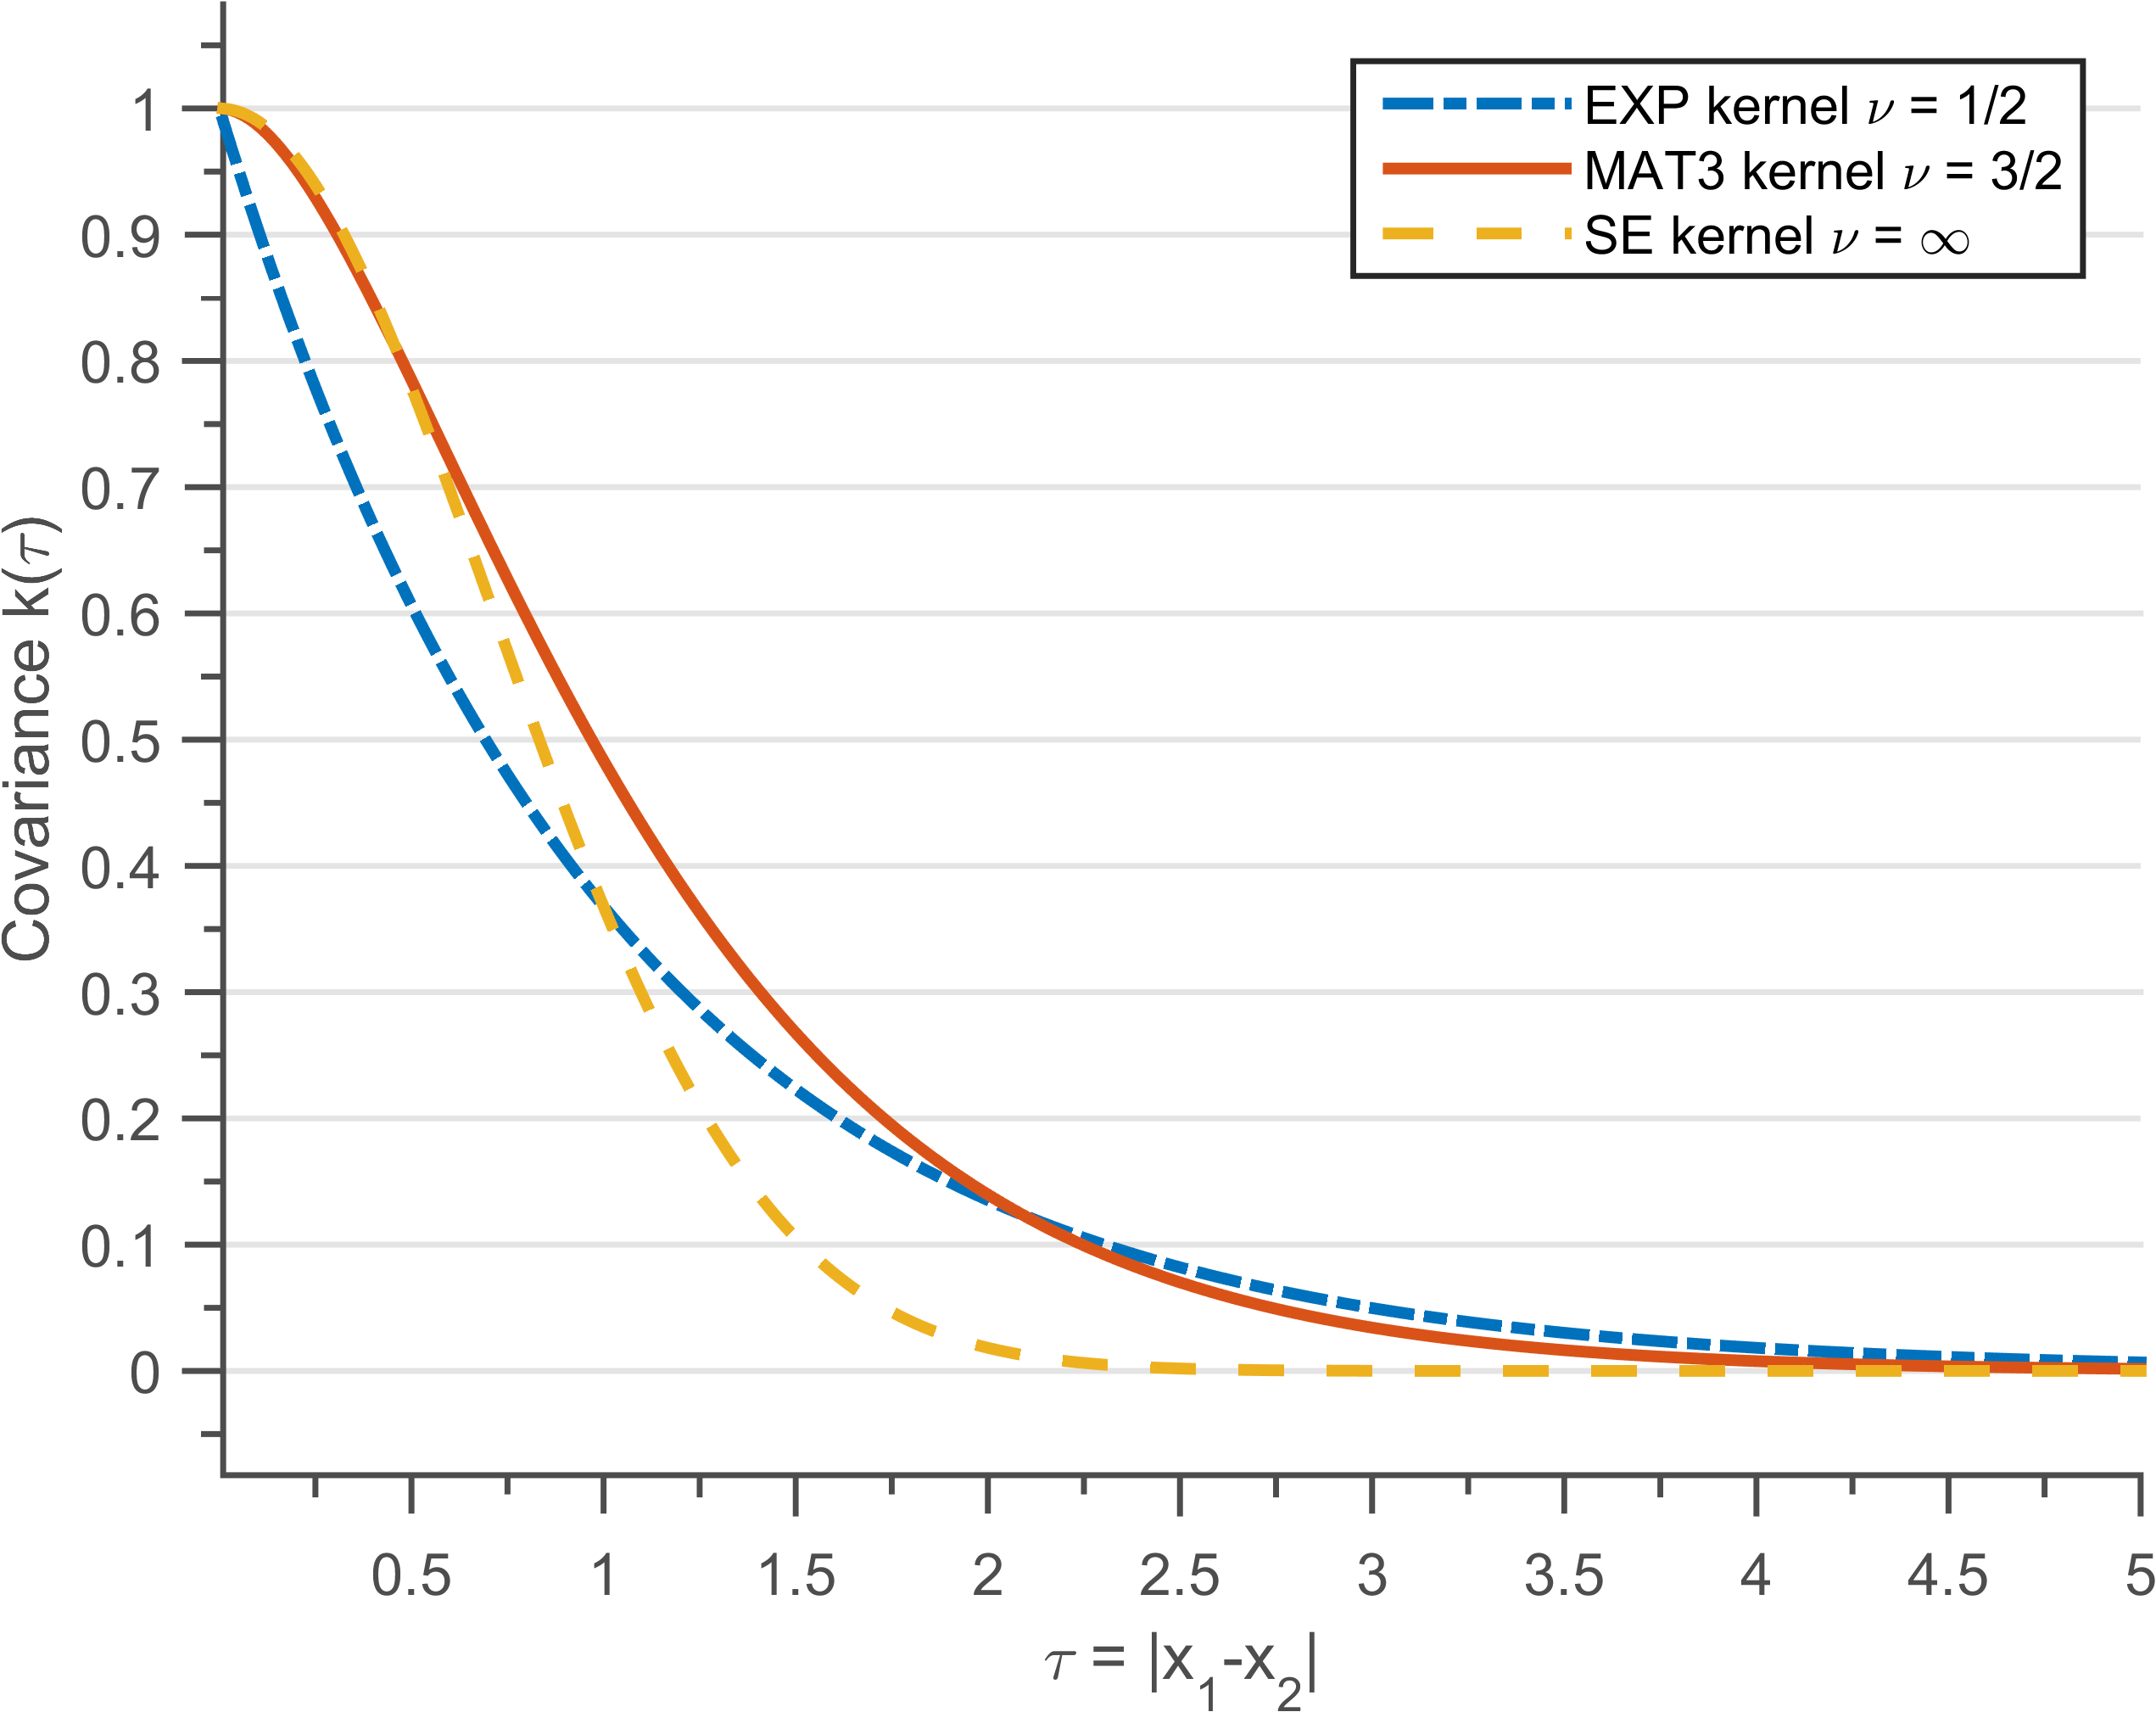
\includegraphics[width=0.45\textwidth]
        {images/part2/kernelFunctions}
        \label{subFigkernelFunctions}
  }\quad
\subfigure[{Power spectrum for Exponential, Mat\'ern ($\nu=3/2$)and SE kernel. The hyper-parameters are amplitude ($\theta_{amplitude} = 1$) and length-scale ($\theta_{lengthScale} = 1$). Exponential and Mat\'ern have more power at higher frequencies when compared to SE kernel.}]
  {
        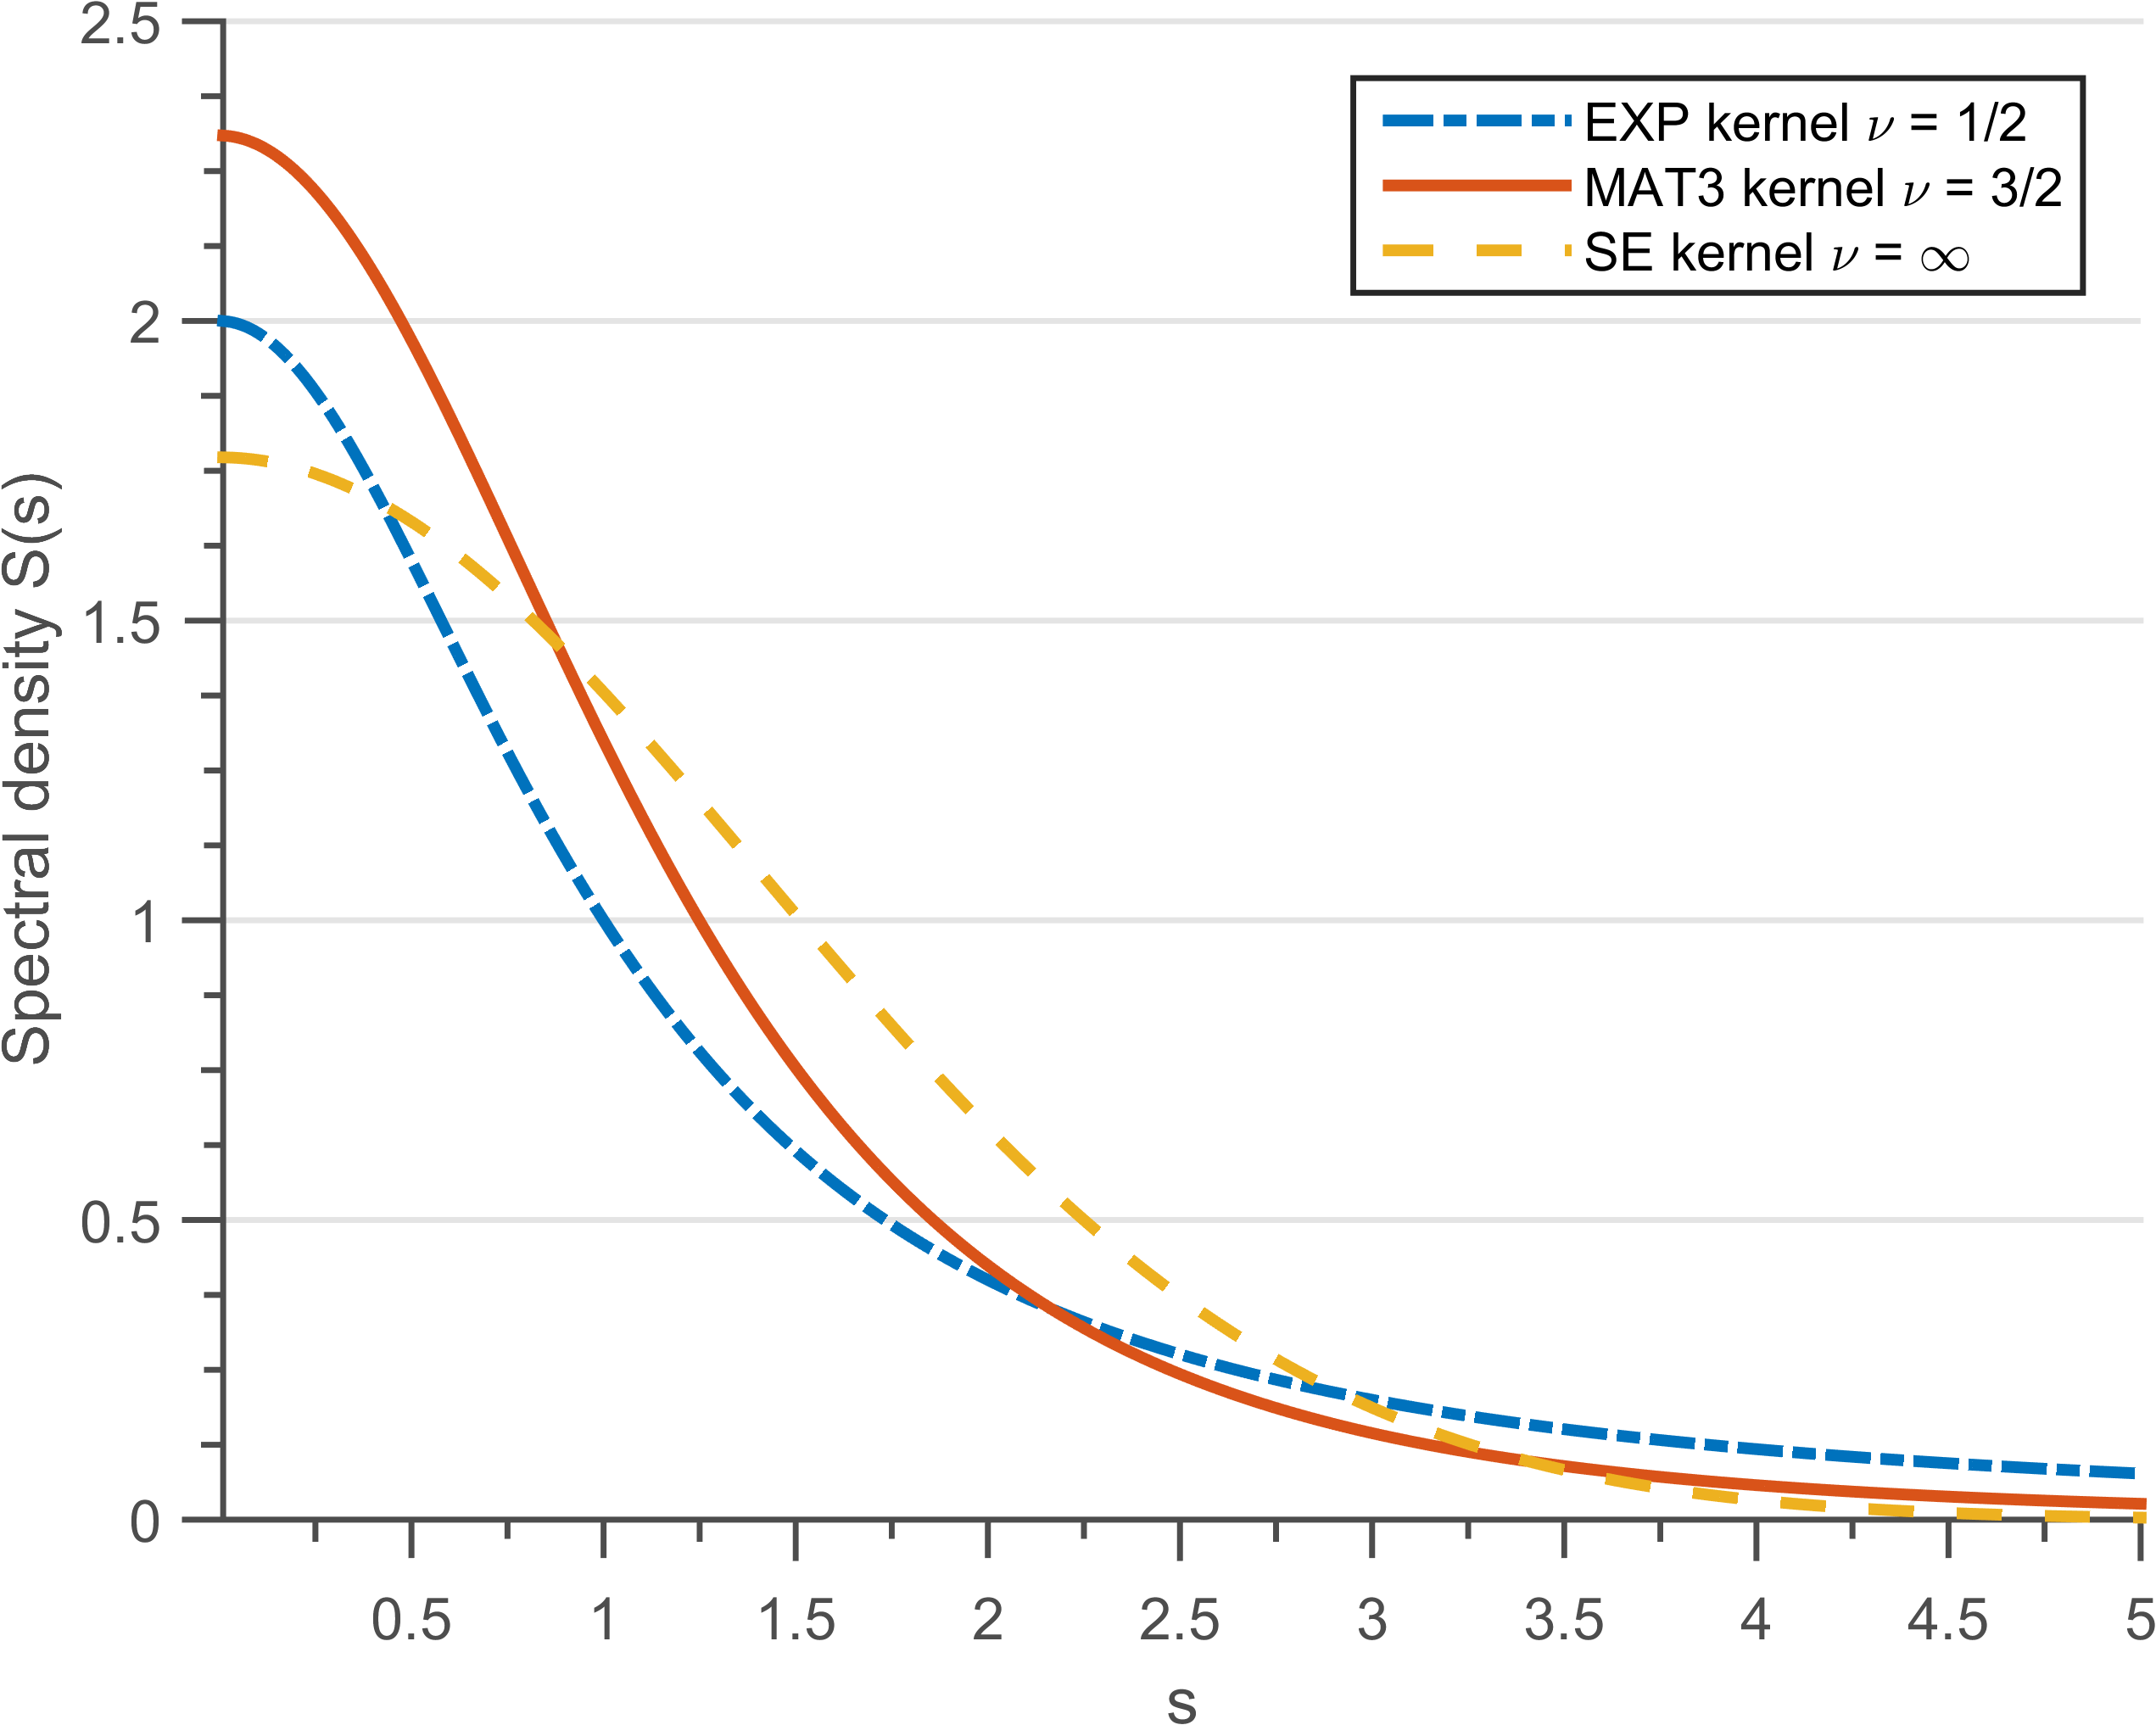
\includegraphics[width=0.45\textwidth]
        {images/part2/spectralFunctions}
        \label{subFigspectralFunctions}
  }\quad
\caption{Covariance functions and Power spectrums for three different kernels}
       \label{figKernelAndPowerSpectrums}
\end{figure}

\subsection{Experiments}\label{subsecCH4Experiments}
\begin{mdframed}[hidealllines=true,backgroundcolor=lightgray!20]
Let us revisit the data-set $\mathcal{D}_{2}$ used to choose the hyper-parameters in section \ref{secPosterior}, but this time using three different covariance functions. We will use Exponential kernel, Mat\'ern ($\nu=1/2$) and SE kernel to compare their performance. 

We follow the standard framework of GP regression; we first draw random functions from the covariance function to judge the hypothesis space, we then calculate the posterior distribution conditioned on data-set $\mathcal{D}_{2}$, and finally optimize the marginal likelihood to compare the final predictions of the three covariance functions. 

Figure \ref{figCh4Priors} shows 5 random functions drawn for a zero mean GP with all the three covariance functions having the same values of hyper-parameters ($\theta_{lengthscale} = 1, \theta_{amplitude} = 1$), their corresponding covariance functions (figure \ref{subFigkernelFunctions}) and power spectrums (figure \ref{subFigspectralFunctions}) are shown in figure \ref{figKernelAndPowerSpectrums}. The solid black line defines the mean function, shaded blue region defines 95\% confidence interval (2$\sigma$) distance away from the mean. The dashed lines represent five functions drawn at random from a GP prior. We can observe that figure \ref{subFigpriorDrawsEXP} draws non-differentiable functions while \ref{subFigpriorDrawsMAT3} and \ref{subFigpriorDrawsSE} draw smoother functions. For the same value of the length-scale, the Mat\'ern ($\nu=3/2$) kernel has higher variation, when compared to the SE kernel.
\end{mdframed}

\begin{figure}[!ht]
  \centering
    \subfigure[{Draws from a GP prior with mean zero, Exponential kernel (Mat\'ern with $\nu = 1/2$) and hyper-parameters $\theta_{lengthscale} = 1, \theta_{amplitude} = 1$. Functions drawn from this kernel are non-differentiable.}]
  {
        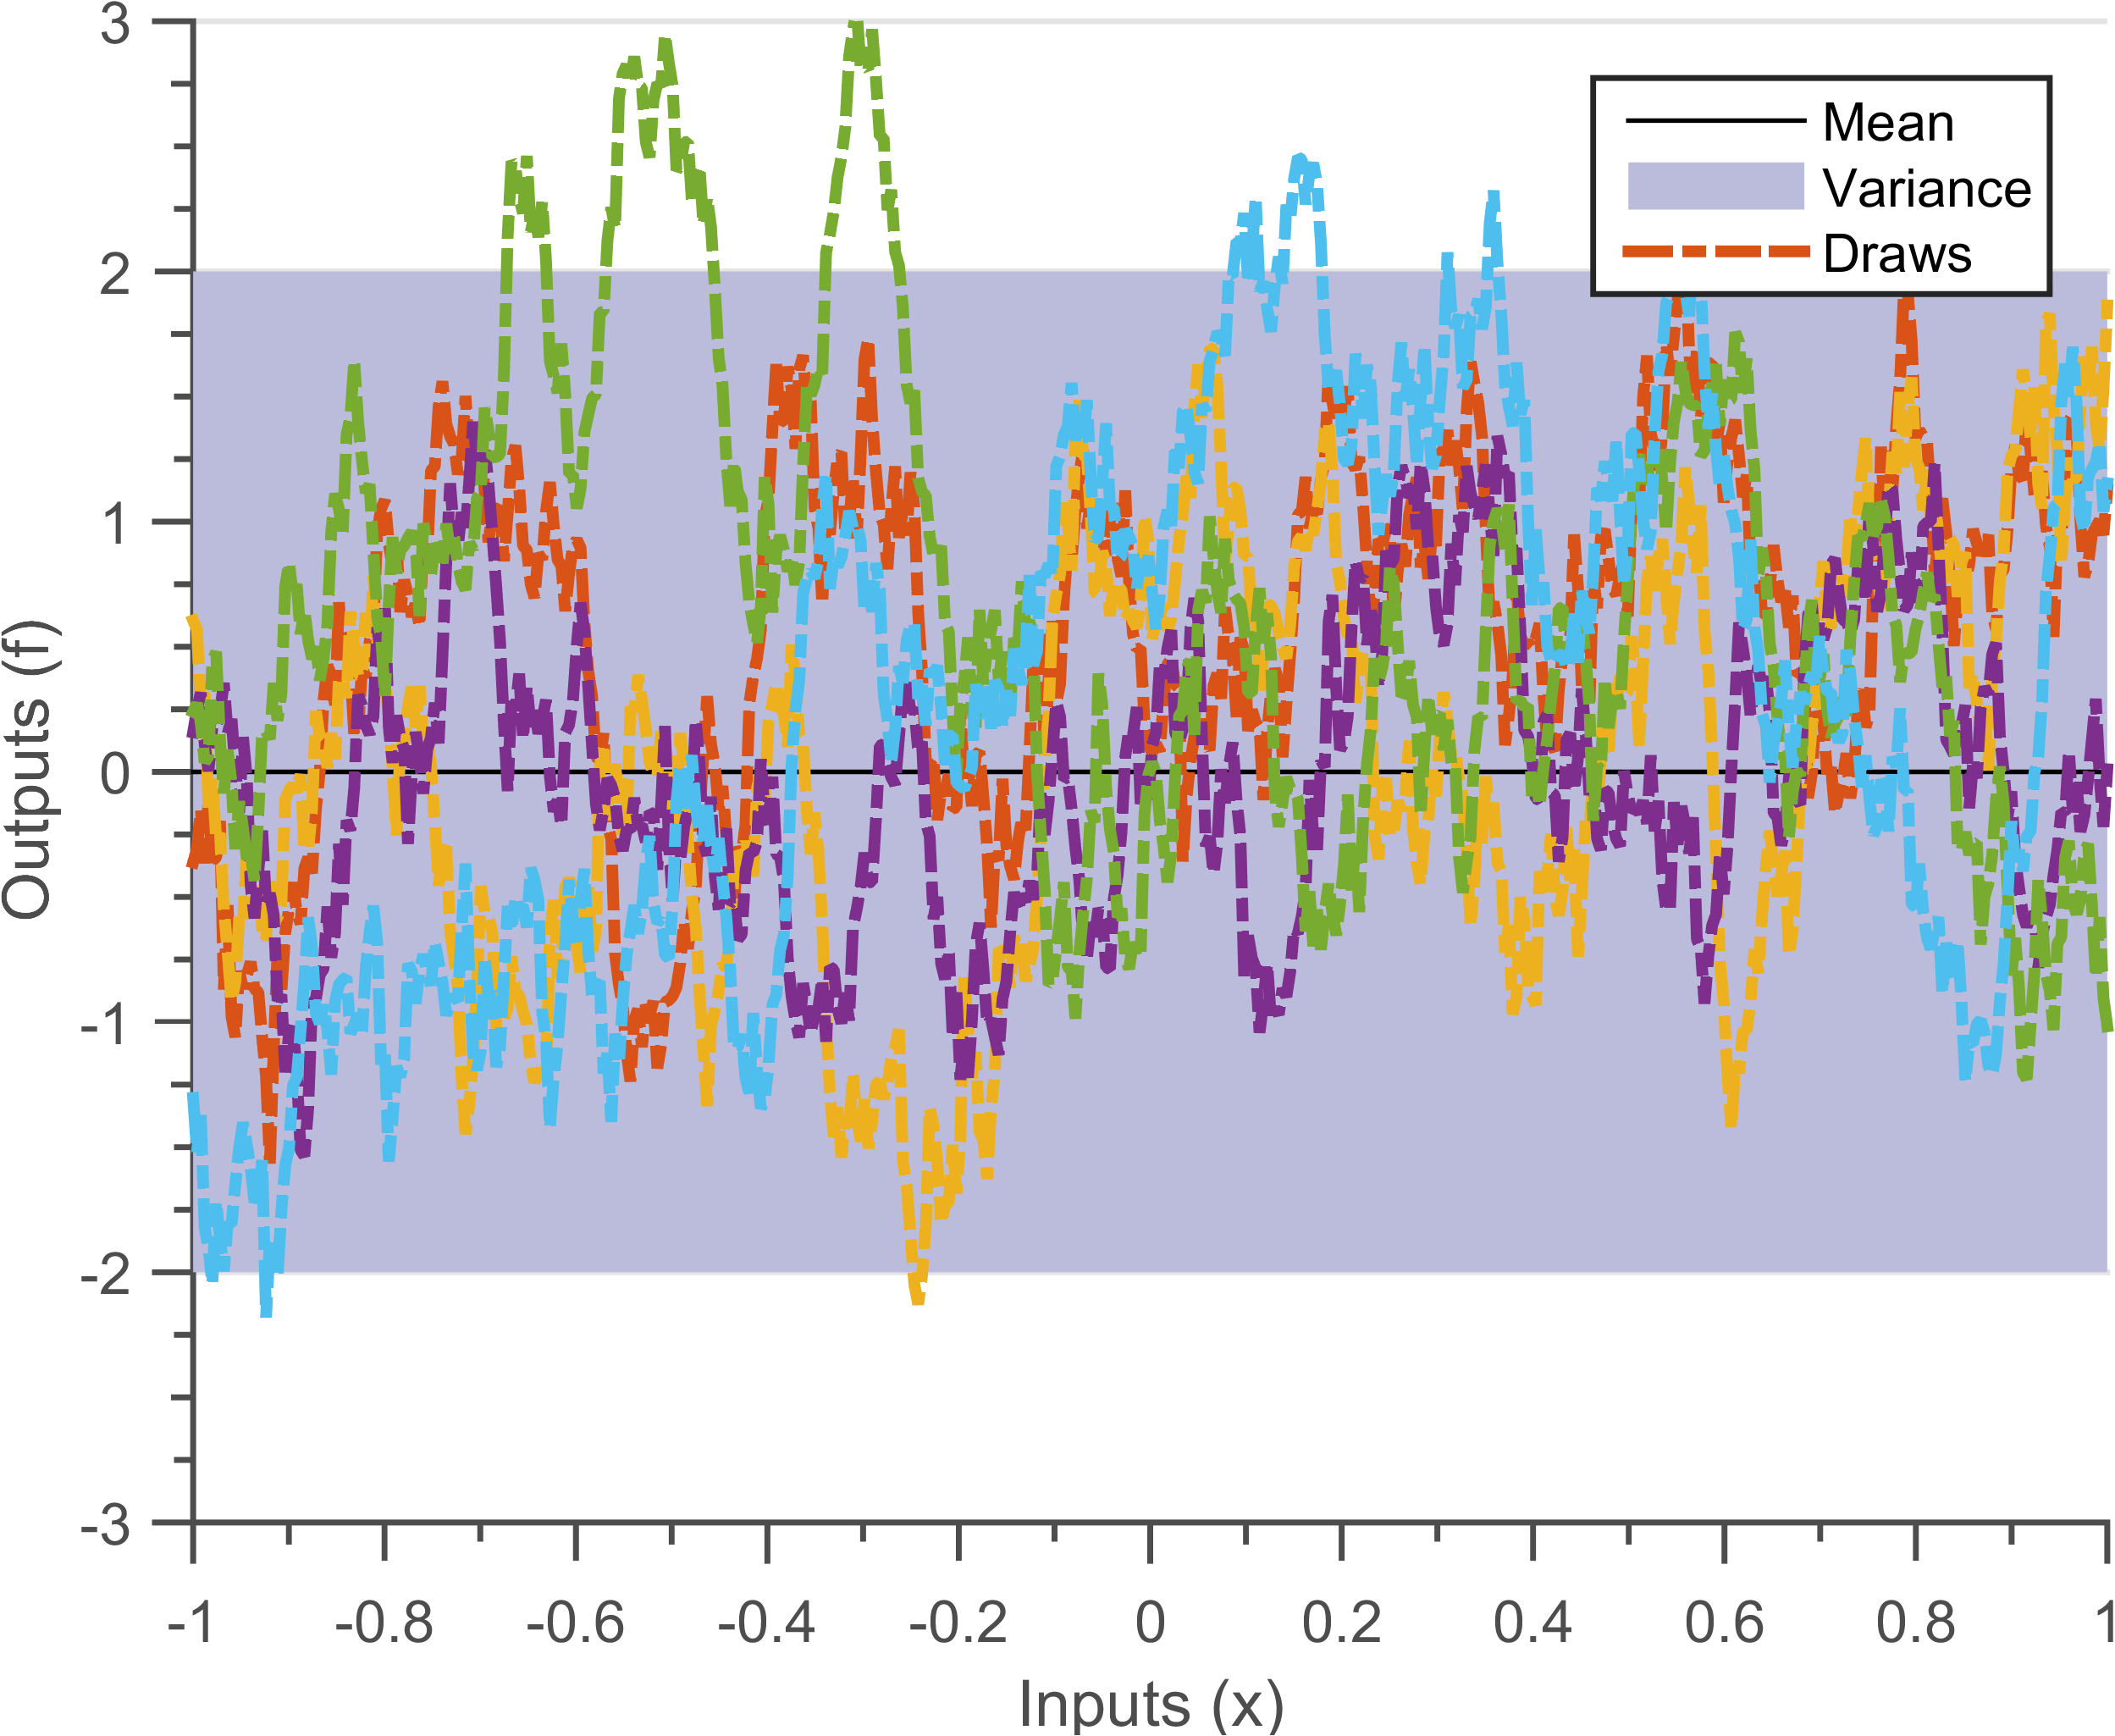
\includegraphics[width=0.29\textwidth]
        {images/part2/priorDrawsEXP}
        \label{subFigpriorDrawsEXP}
  }\quad
\subfigure[{Draws from a GP prior with mean zero, Mat\'ern kernel $\nu = 3/2$ and hyper-parameters $\theta_{lengthscale} = 1, \theta_{amplitude} = 1$. Functions drawn from this kernel are differentiable only once}]
  {
        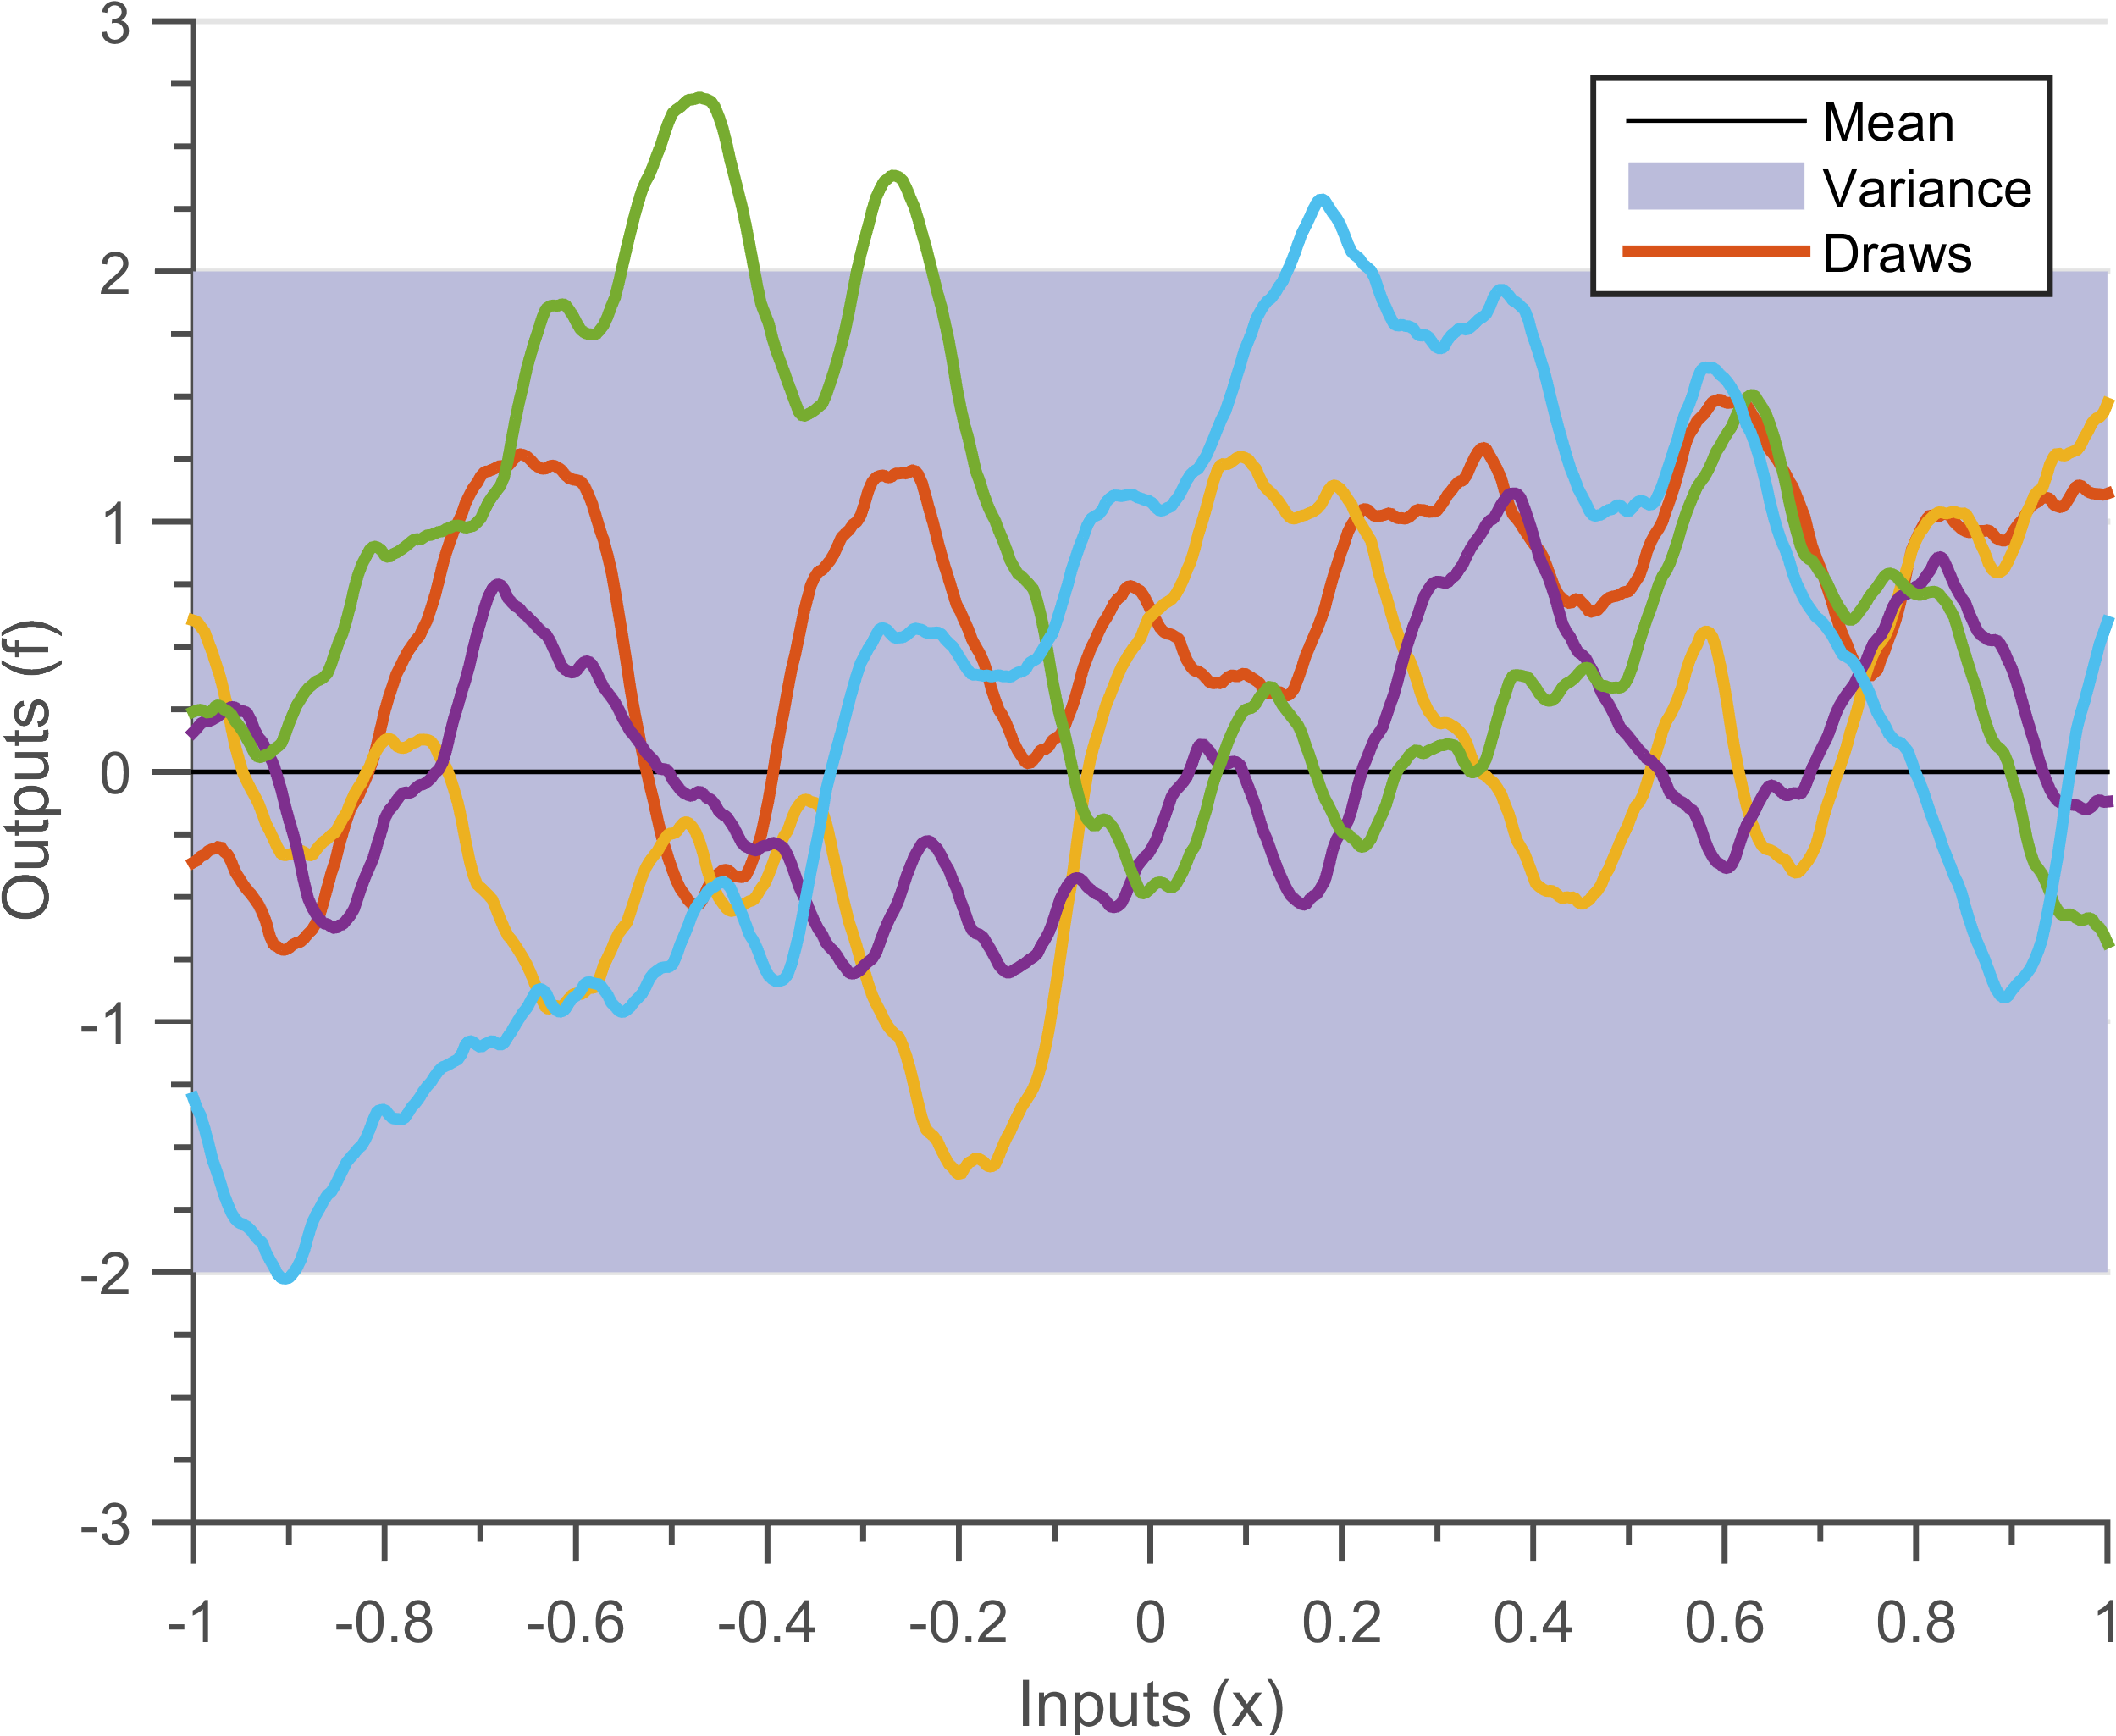
\includegraphics[width=0.29\textwidth]
        {images/part2/priorDrawsMAT3}
        \label{subFigpriorDrawsMAT3}
  }\quad
  \subfigure[{Draws from a GP prior with mean zero, SE kernel (Mat\'ern with $\nu = \infty$) and hyper-parameters $\theta_{lengthscale} = 1, \theta_{amplitude} = 1$. Functions drawn from this kernel are infinitely differentiable}]
  {
        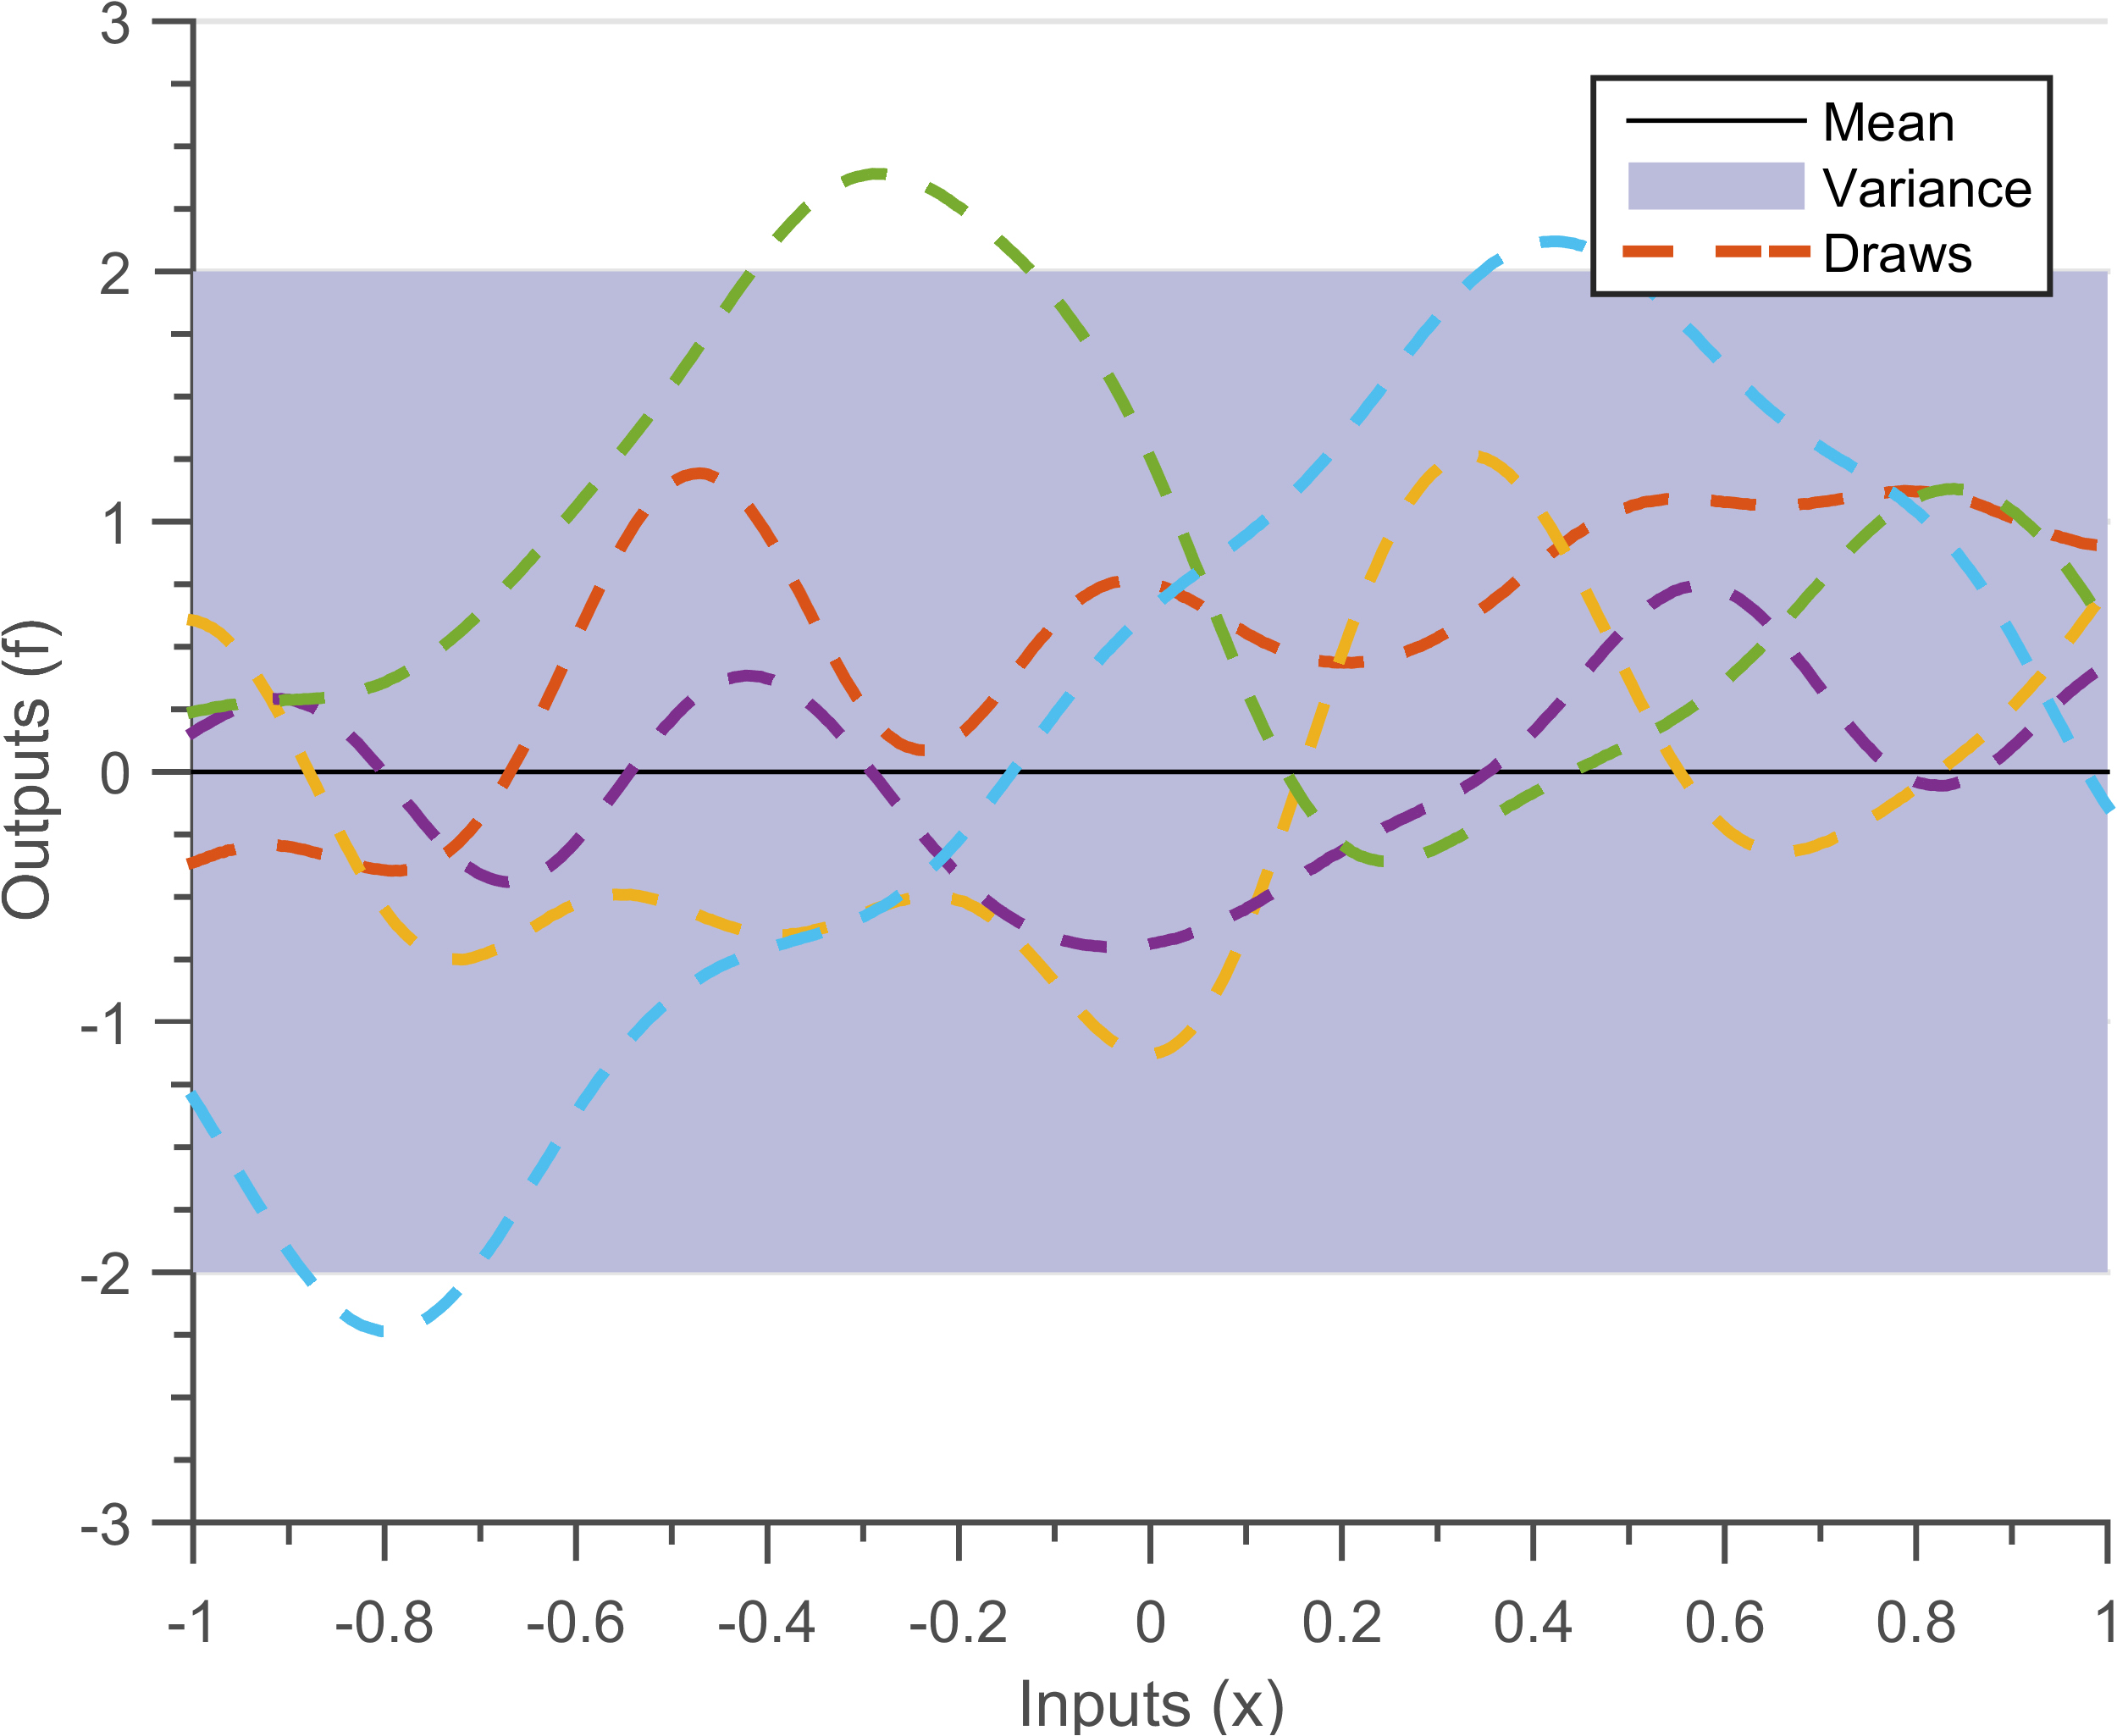
\includegraphics[width=0.29\textwidth]
        {images/part2/priorDrawsSE}
        \label{subFigpriorDrawsSE}
  }\quad
\caption{Prior distribution and five random draws from 3 different covariance functions. The solid black line defines the mean function, shaded blue region defines 95\% confidence interval (2$\sigma$) distance away from the mean. The dashed lines represent five functions drawn at random from a GP prior.}
       \label{figCh4Priors}
\end{figure}

\begin{mdframed}[hidealllines=true,backgroundcolor=lightgray!20]
Figure \ref{figpreOptimizedPosteriorCh5} shows the posterior GP conditioned on the data-set $\mathcal{D}_{2}$ for three different covariance functions with the same hyper-parameters, these hyper-parameters are not optimized with respect to the marginal likelihood. For similar values of hyper-parameters and data-set, Exponential kernel has highest variance followed by Mat\'ern and SE kernel. This is a consequence of the bias vs variance trade-off since the SE kernel has the most restrictive hypothesis space (infinite differentiability is a stricter assumption), followed by Mat\'ern $\nu=3/2$ and Exponential kernel.
\end{mdframed}

\begin{figure}[!ht]
  \centering
    \subfigure[{Draws from a GP posterior with mean zero and Exopnential kernel (figure \ref{subFigpriorDrawsEXP}) conditioned on the data $\mathcal{D}_{2}$. The posterior mean passes through the data points, random functions drawn from exponential kernel are non-differentiable}]
  {
        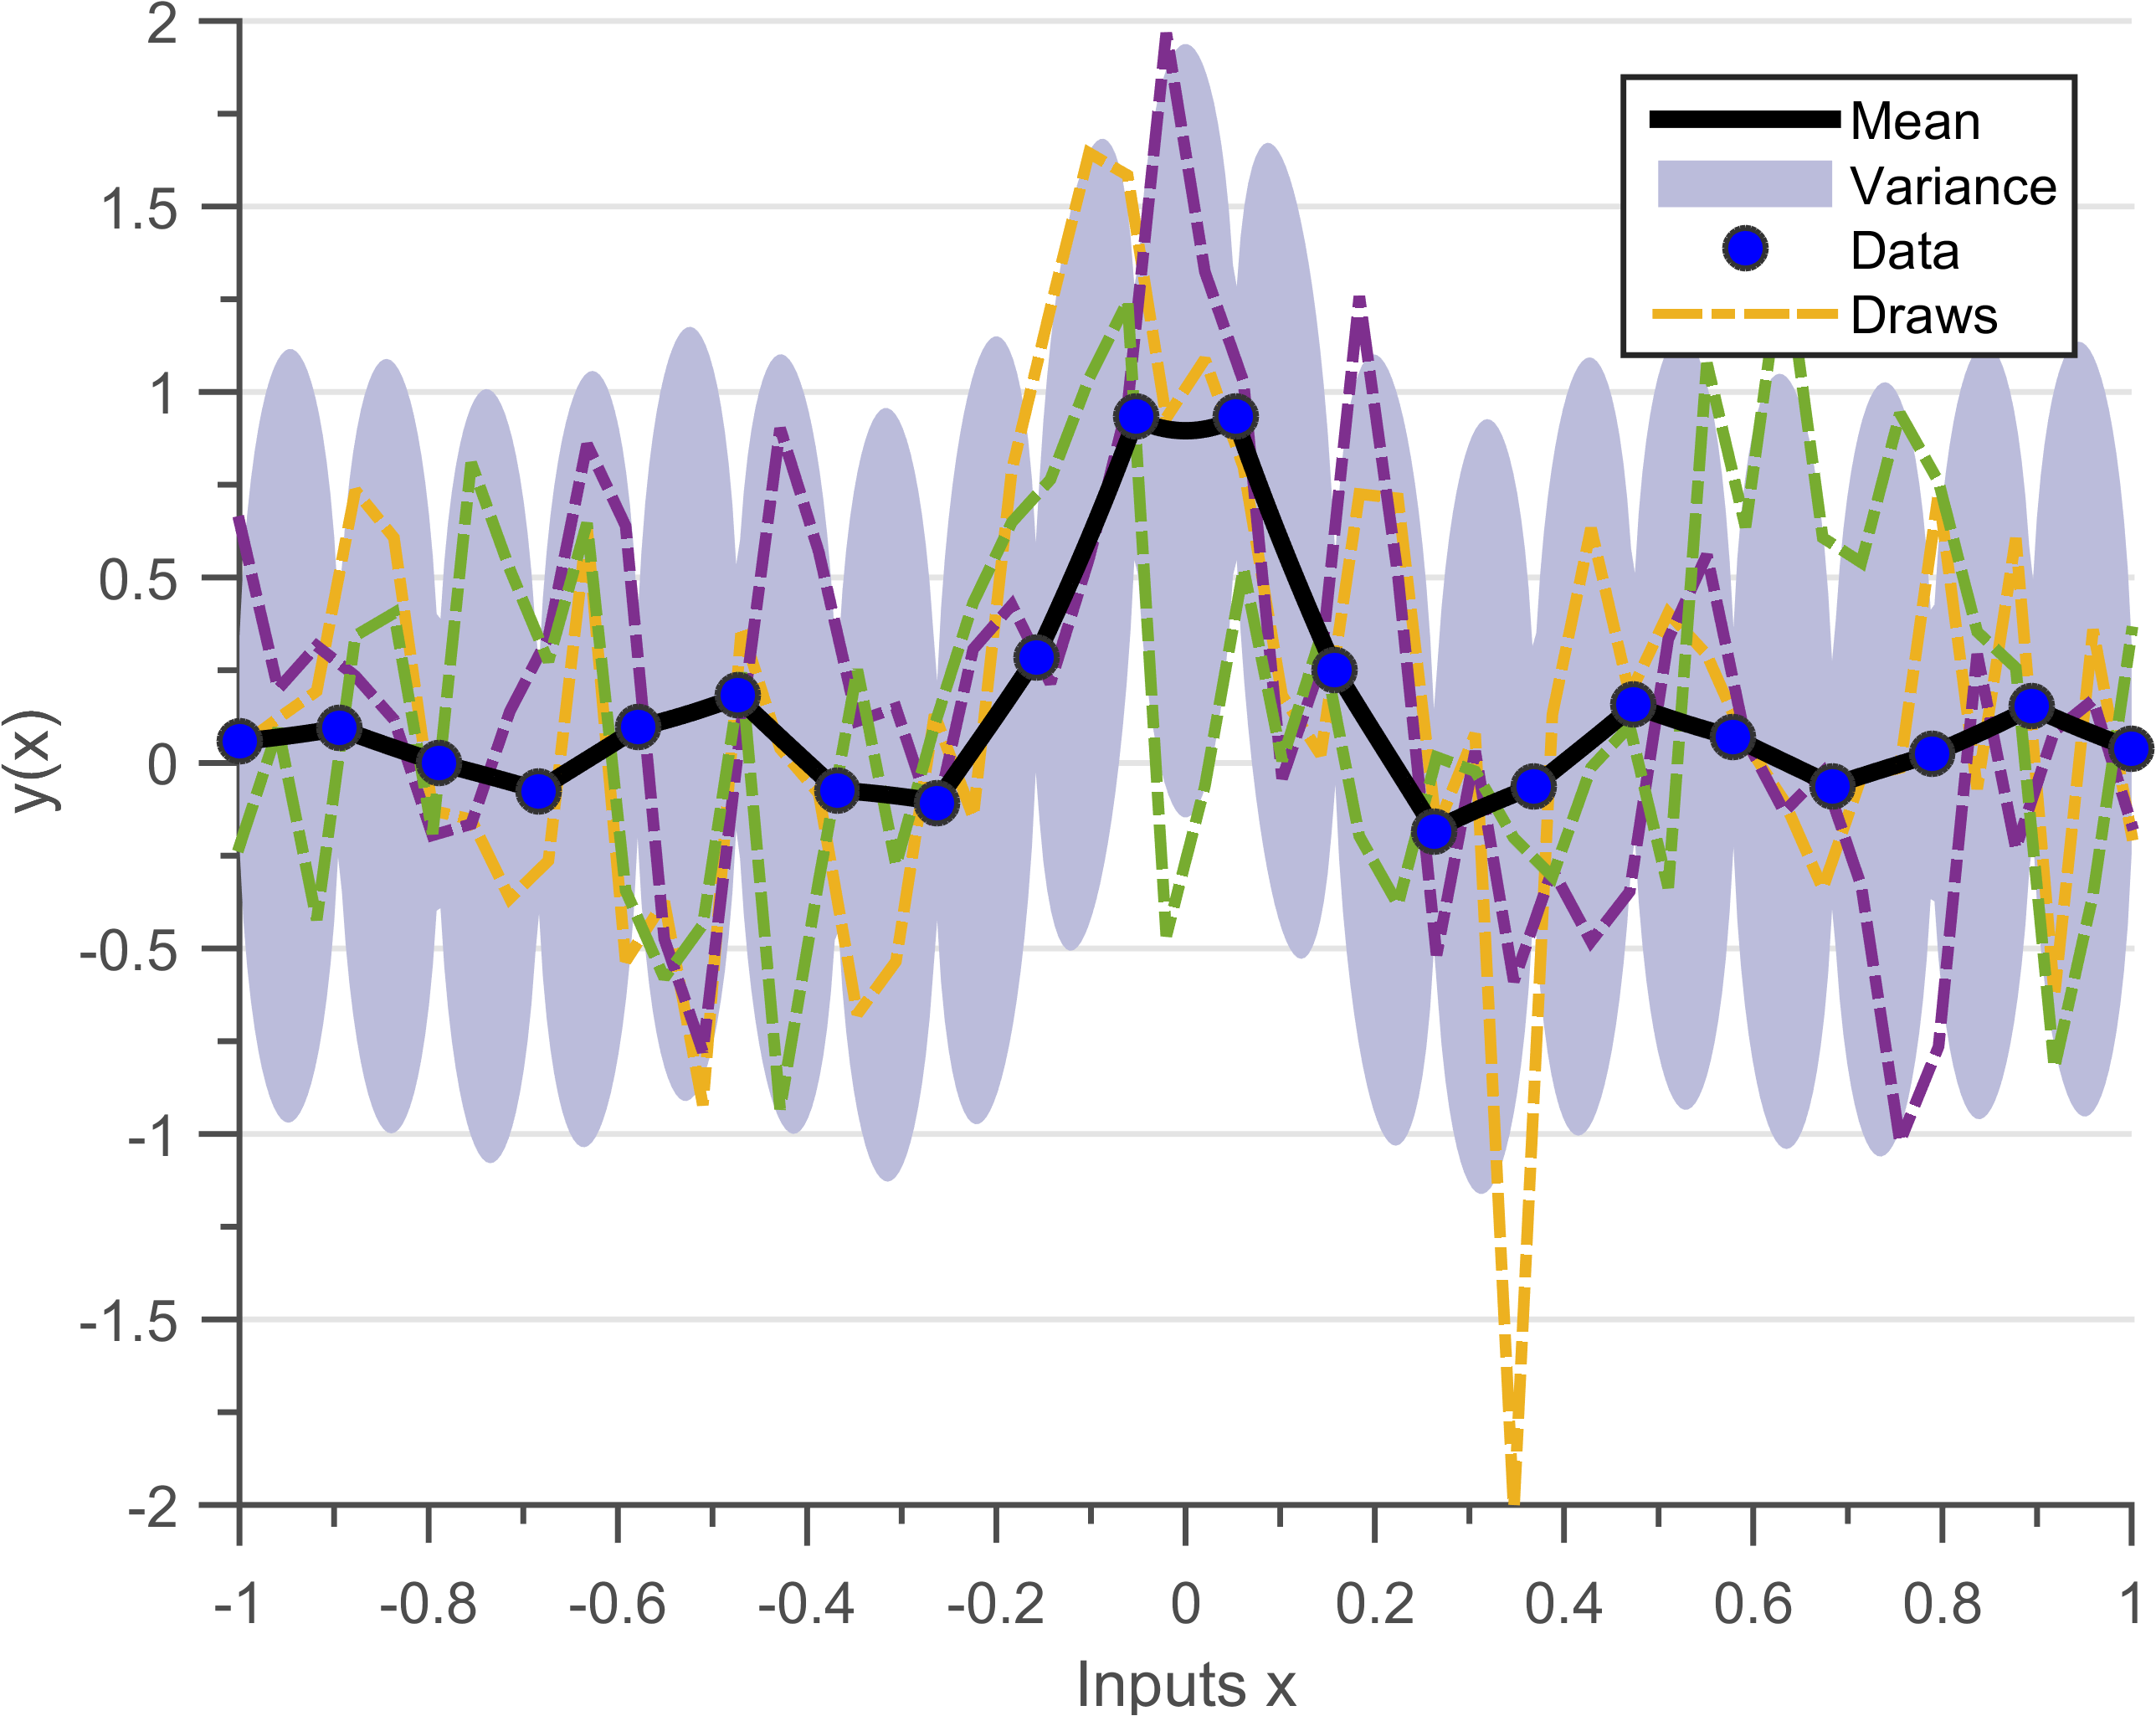
\includegraphics[width=0.29\textwidth]
        {images/part2/drawsPosteriorEXP}
        \label{subFigdrawsPosteriorEXP}
  }\quad
\subfigure[{Draws from a GP posterior with mean zero and Mat\'ern kernel $\nu = 3/2$ (figure \ref{subFigpriorDrawsMAT3}) conditioned on the data $\mathcal{D}_{2}$. The posterior mean passes through the data points, random functions drawn from this kernel are differentiable only once}]
  {
        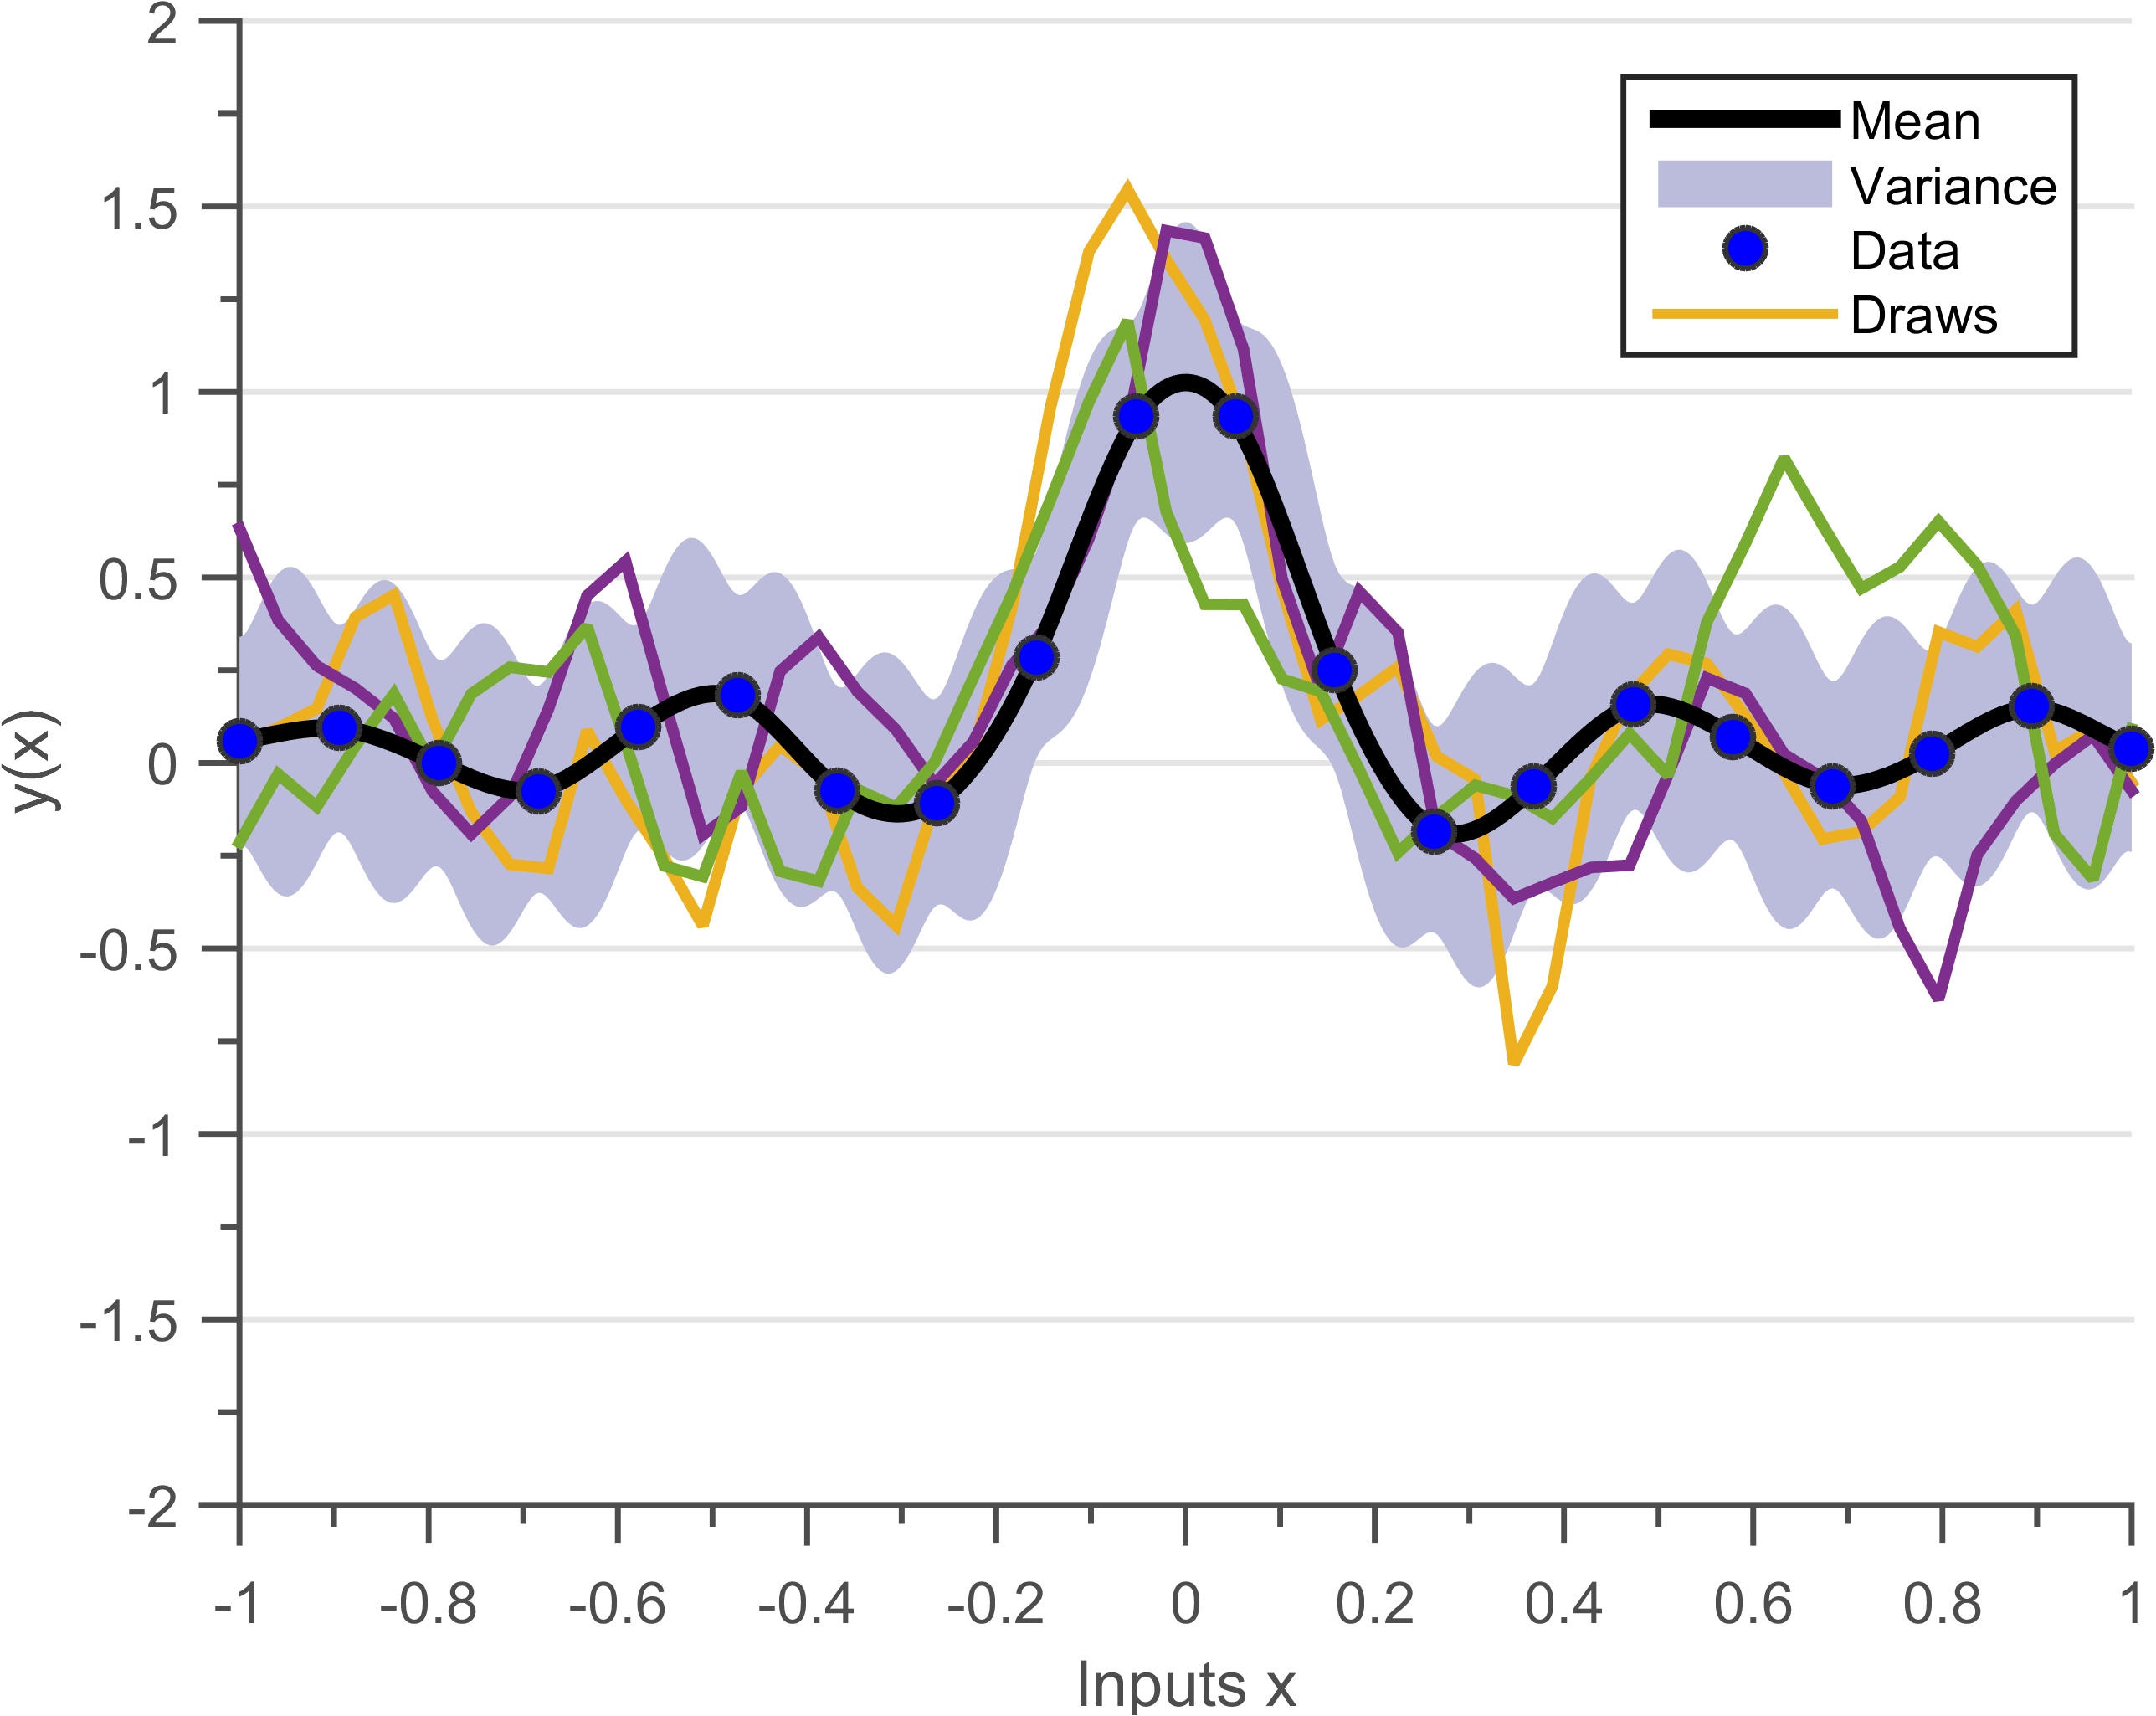
\includegraphics[width=0.29\textwidth]
        {images/part2/drawsPosteriorMAT3}
        \label{subFigdrawsPosteriorMAT3}
  }\quad
  \subfigure[{Draws from a GP posterior with mean zero and SE kernel $\nu = \infty$ (figure \ref{subFigpriorDrawsMAT3}) conditioned on the data $\mathcal{D}_{2}$. The posterior mean passes through the data points, random functions drawn from exponential kernel are infinitely differentiable}]
  {
        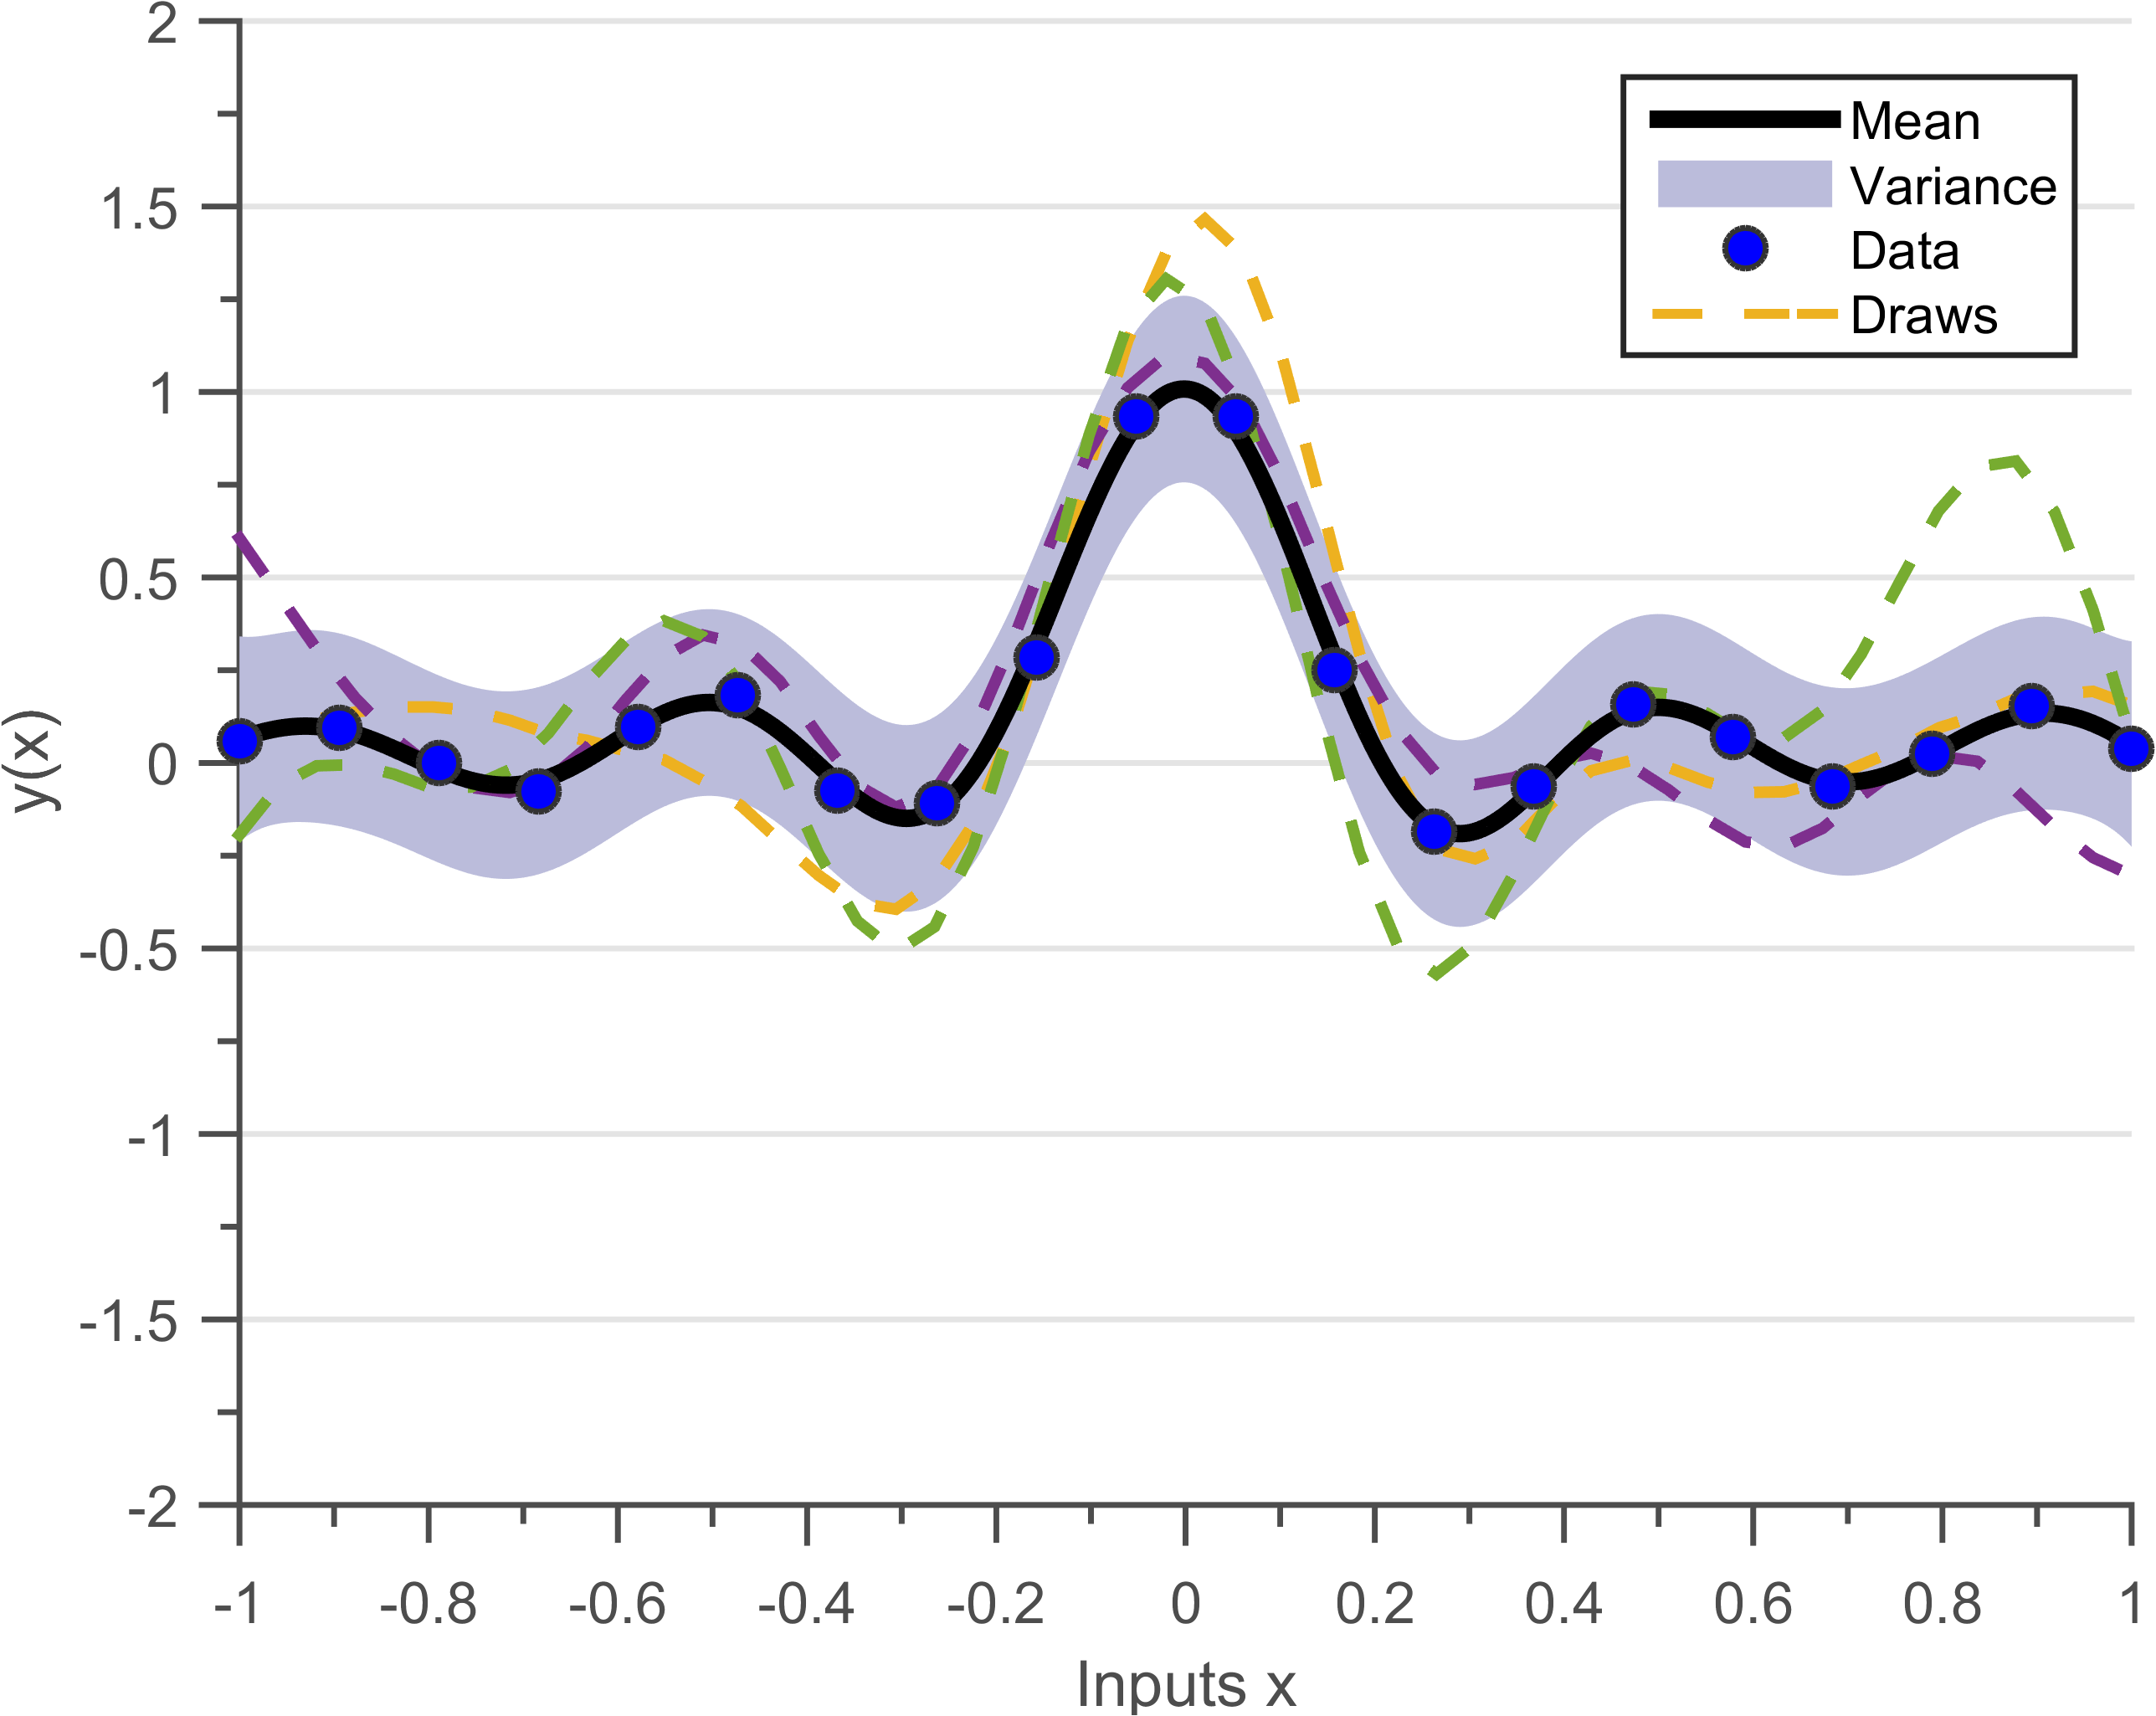
\includegraphics[width=0.29\textwidth]
        {images/part2/drawsPosteriorSE}
        \label{subFigdrawsPosteriorSE}
  }\quad
\caption{Posterior distribution and three random draws from 3 different covariance functions. The solid black line defines the mean function, shaded blue region defines 95\% confidence interval (2$\sigma$) distance away from the mean. The dashed lines represent five functions drawn at random from a GP prior. }
       \label{figpreOptimizedPosteriorCh5}
\end{figure}

\begin{mdframed}[hidealllines=true,backgroundcolor=lightgray!20]
Figure \ref{figOptimizedPosteriorCh4} shows the posterior GP conditioned on the data-set $\mathcal{D}_{2}$, for three different covariance functions with optimized hyper-parameters. All the three covariance functions estimate the same value of amplitude hyper-parameter, while having significantly different value of noise hyper-parameter (lowest noise estimated for Exponential kernel followed by Mat\'ern ($\nu=3/2$) and SE kernel). 

\marginnote{\textsl{Bias vs Variance}}[1cm]
The Exponential kernel defines a family of non-differentiable functions, hence functions in its hypothesis space have the flexibility to pass through all the data-points. Whereas, the SE kernel has less flexibility in the functions in its hypothesis space, due to its strict bias (infinitely differentiable). If the data-set does not have the same level of smoothness the SE kernel will find the closest function in its hypothesis space, and associate the difference to noise. Hence the Exponential kernel will almost always have a low noise estimate than the SE kernel. The infinitely smooth assumption of the squared exponential function is unrealistic in several cases, making the Mat\'ern kernels ($\nu=5/2$) second most popular choice of kernels \cite{Stein1999Springer, cornford2002modelling}. 

\marginnote{\textsl{Engineering judgment}}[1cm]
This experiment only shows the different posteriors obtained for the same observational data and different functional forms of the covariance function. All three predictions can be the correct interpolations depending on the type of experiment, this is where engineering judgment is required. For example, if the data-set $\mathcal{D}_{2}$ was measured from a Brownian motion experiment then figure \ref{subFigdrawsOptimizedPosteriorEXP} would be the best fit, since the exponential kernel encodes prior information of Brownian motion (section \ref{subsecCh4MaternKernel}).

\end{mdframed}

\begin{figure}[!ht]
  \centering
    \subfigure[{Draws from a GP posterior, conditioned on the data-set $\mathcal{D}_{1}$ with mean zero and Exponential kernel with hyper-parameters ($\theta_{lengthscale} = 0.215$, $\theta_{amplitude} = 0.312$ and $\sigma_{n} = 2.8e^-5$) that maximize the marginal likelihood ($max(ML) = -1$).}]
  {
        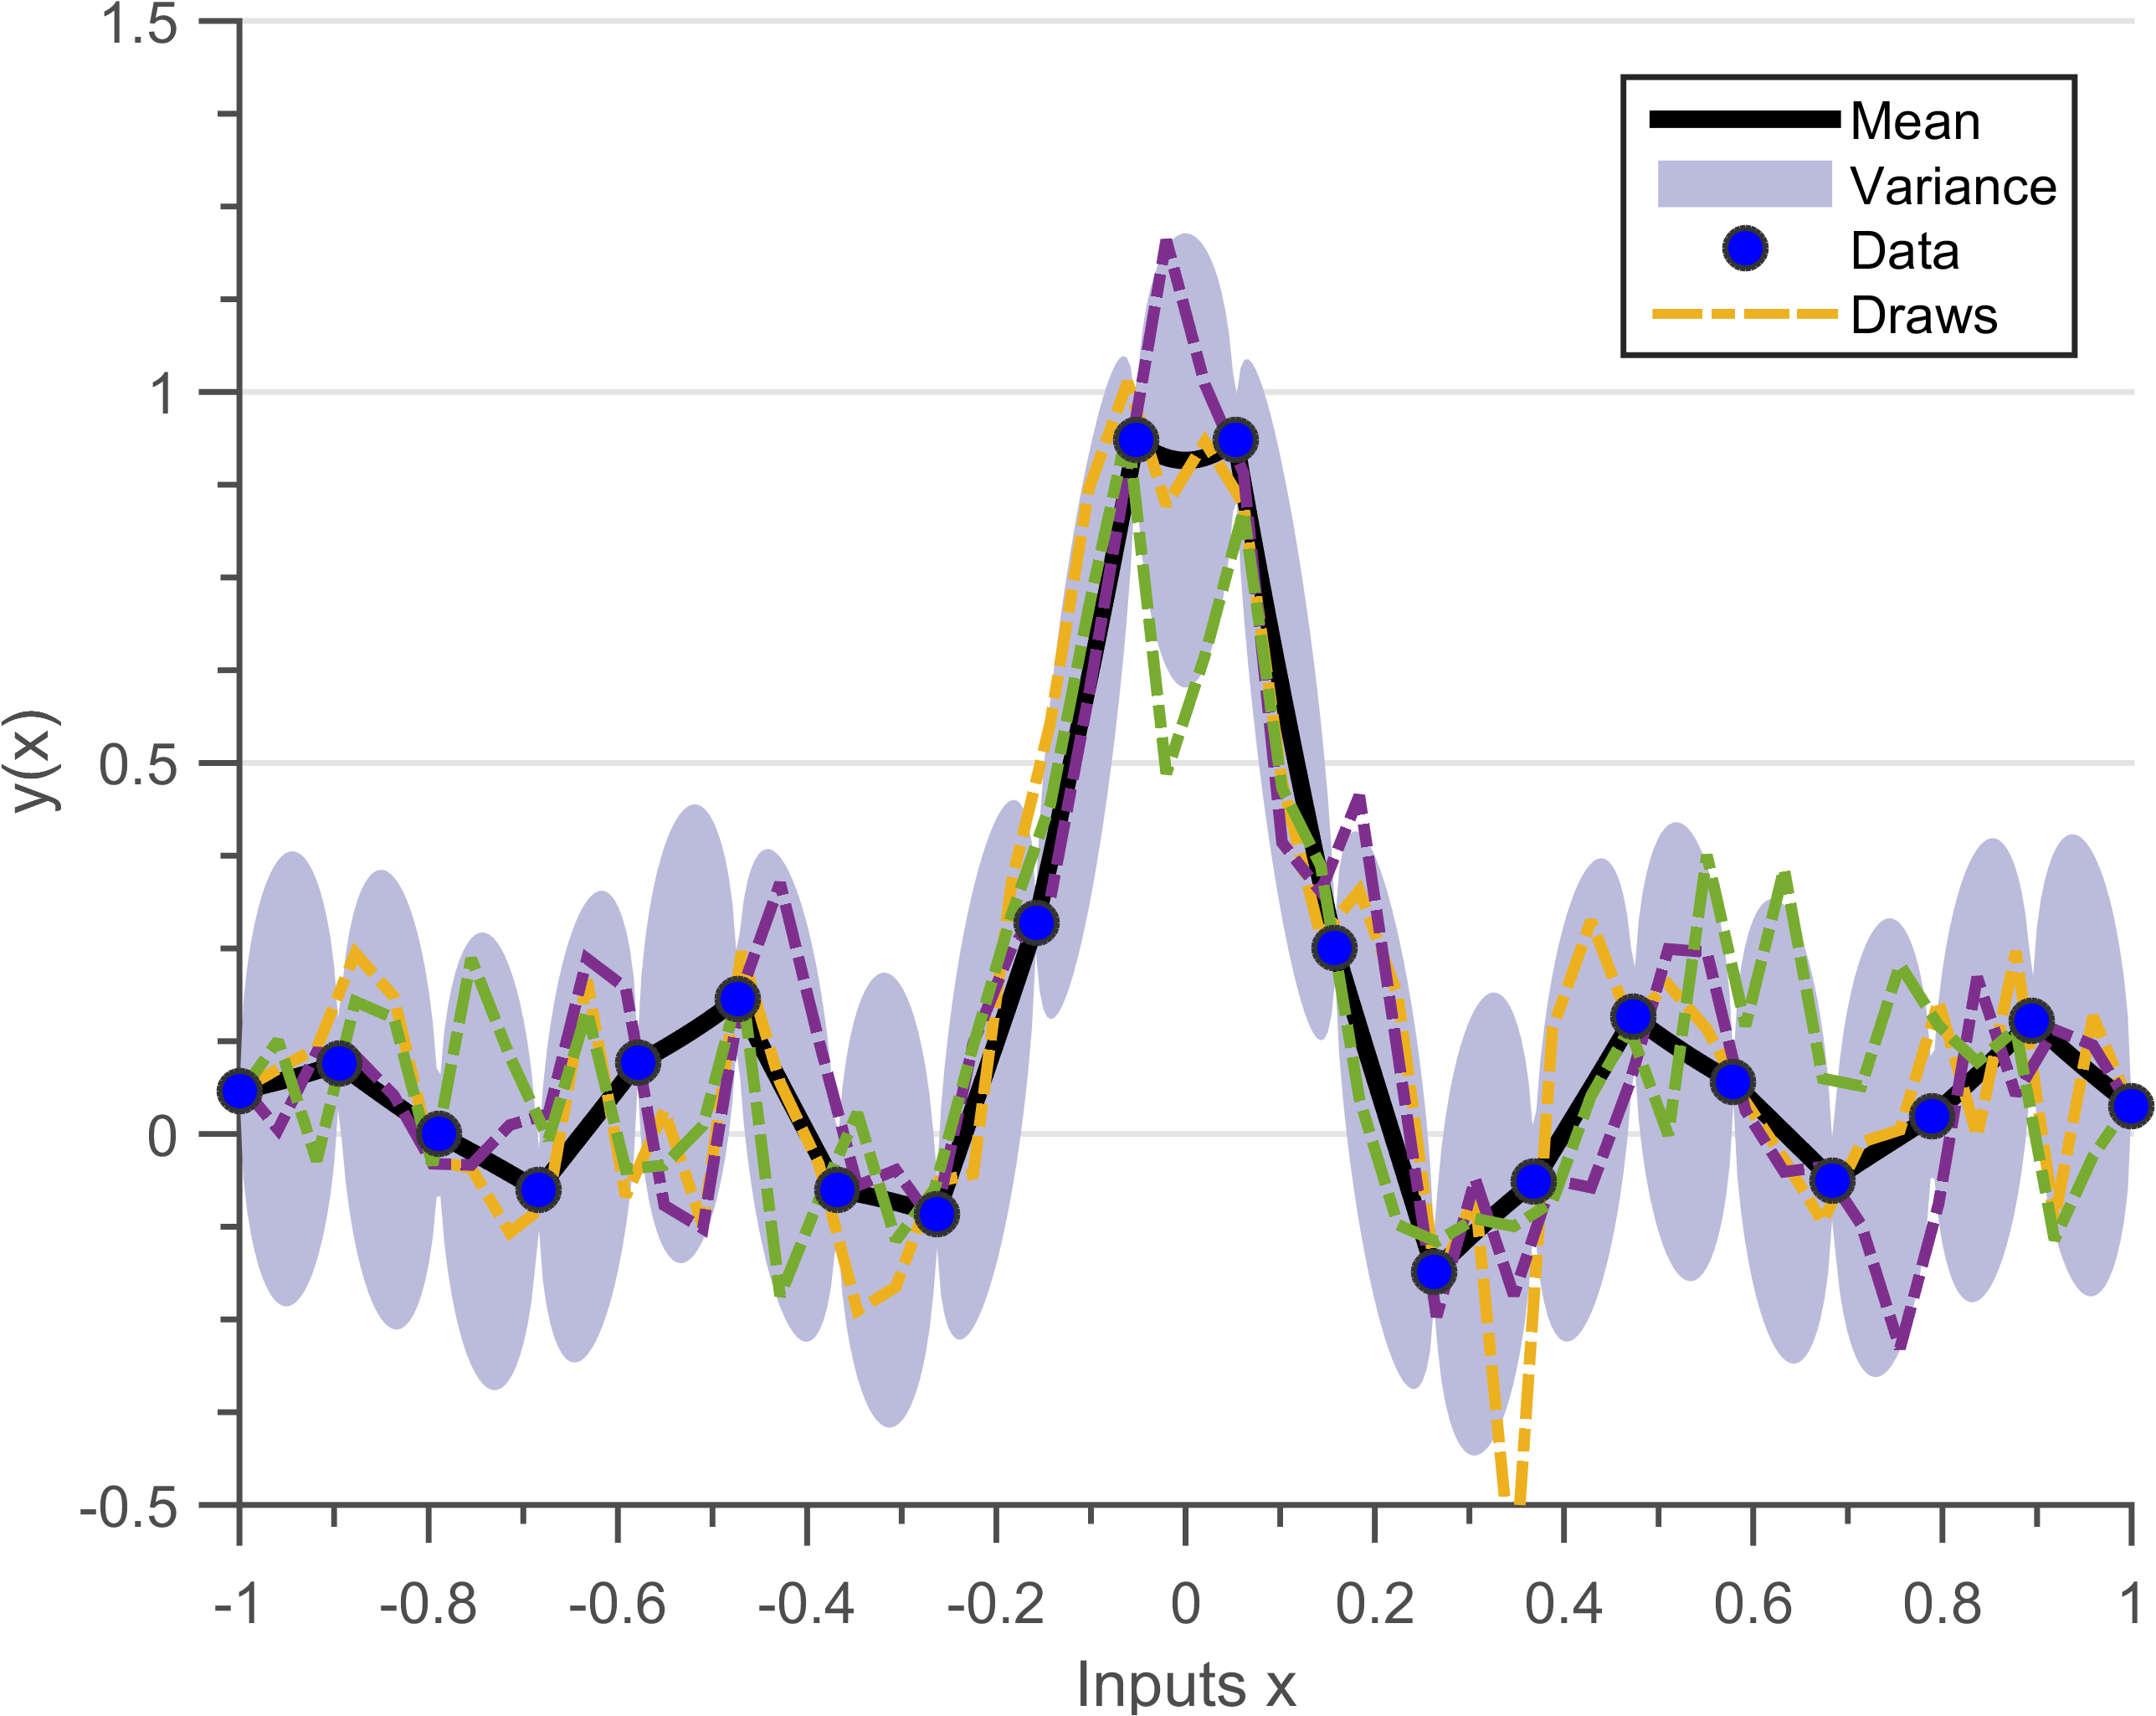
\includegraphics[width=0.29\textwidth]
        {images/part2/drawsOptimizedPosteriorEXP}
        \label{subFigdrawsOptimizedPosteriorEXP}
  }\quad
\subfigure[{Draws from a GP posterior, conditioned on the data-set $\mathcal{D}_{1}$ with mean zero and Mat\'ern ($\nu=3/2$) kernel with hyper-parameters ($\theta_{lengthscale} = 0.2$, $\theta_{amplitude} = 0.347$ and $\sigma_{n} = 1.7e^-5$) that maximize the marginal likelihood ($max(ML) = 2$).}]
  {
        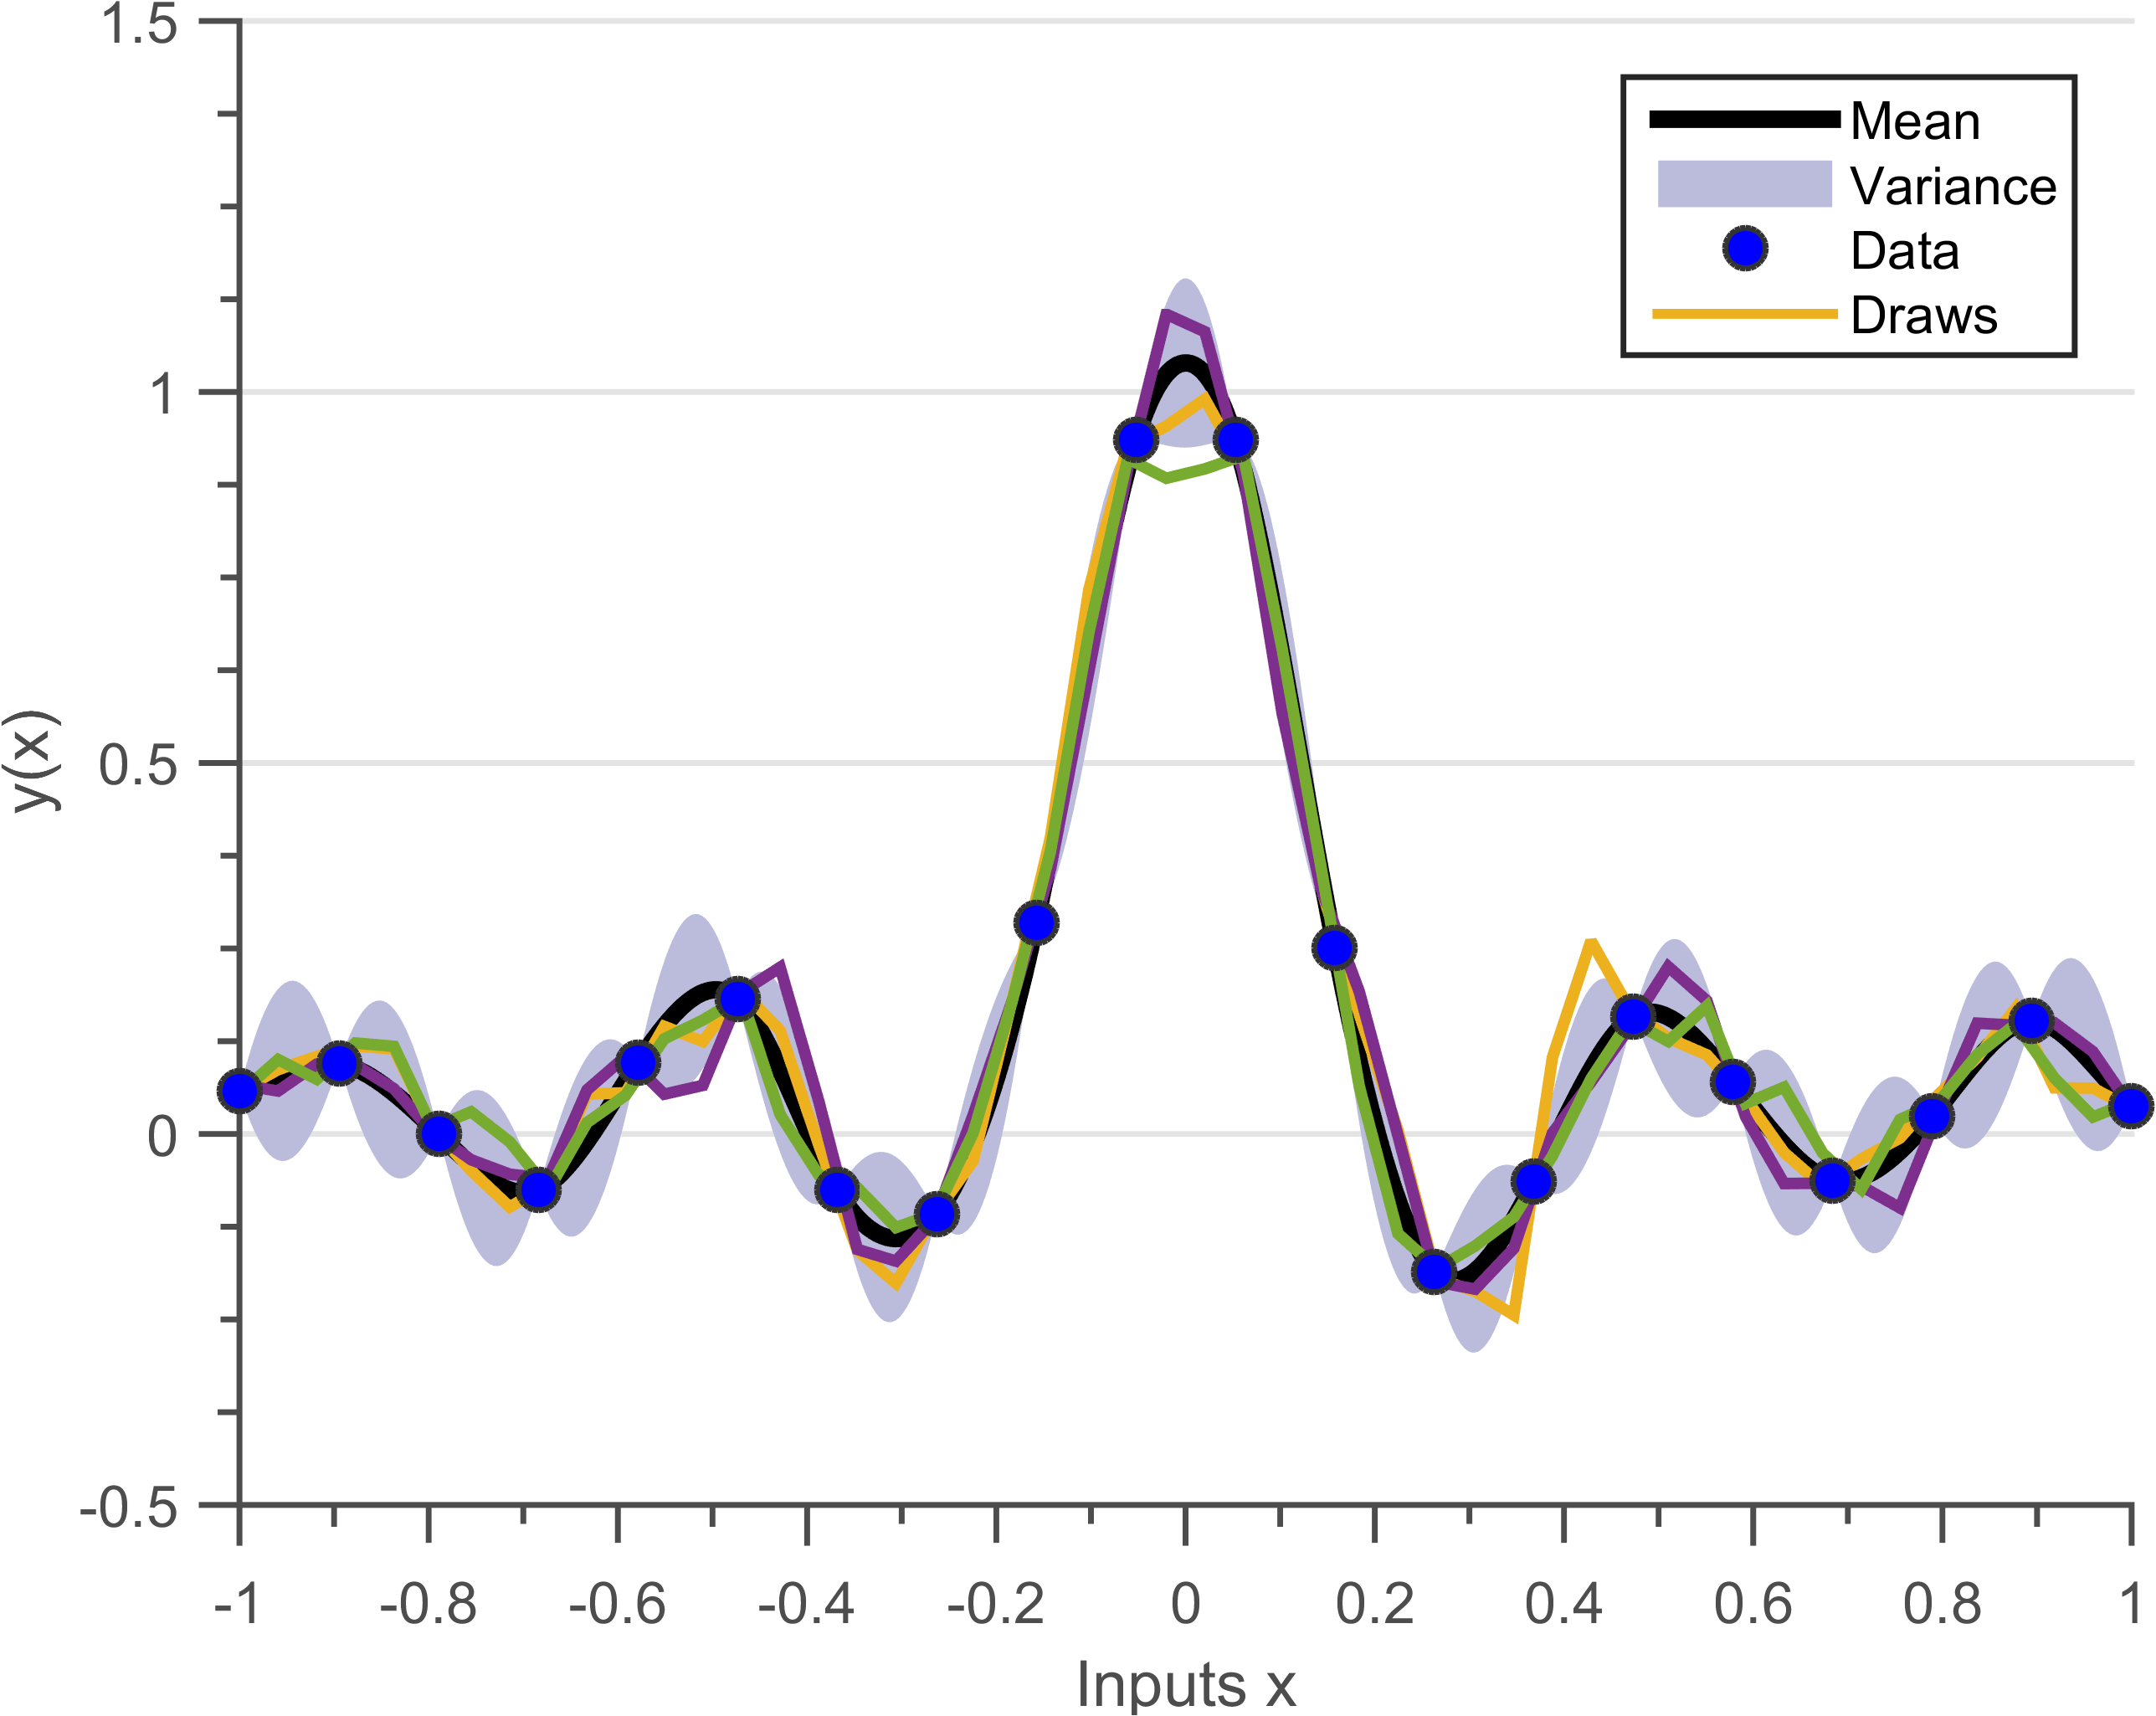
\includegraphics[width=0.29\textwidth]
        {images/part2/drawsOptimizedPosteriorMAT3}
        \label{subFigdrawsOptimizedPosteriorMAT3}
  }\quad
  \subfigure[{Draws from a GP posterior, conditioned on the data-set $\mathcal{D}_{1}$ with mean zero and se kernel with hyper-parameters ($\theta_{lengthscale} = 0.151$, $\theta_{amplitude} = 0.358$ and $\sigma_{n} = 0.01$) that maximize the marginal likelihood ($max(ML) = 8$).}]
  {
        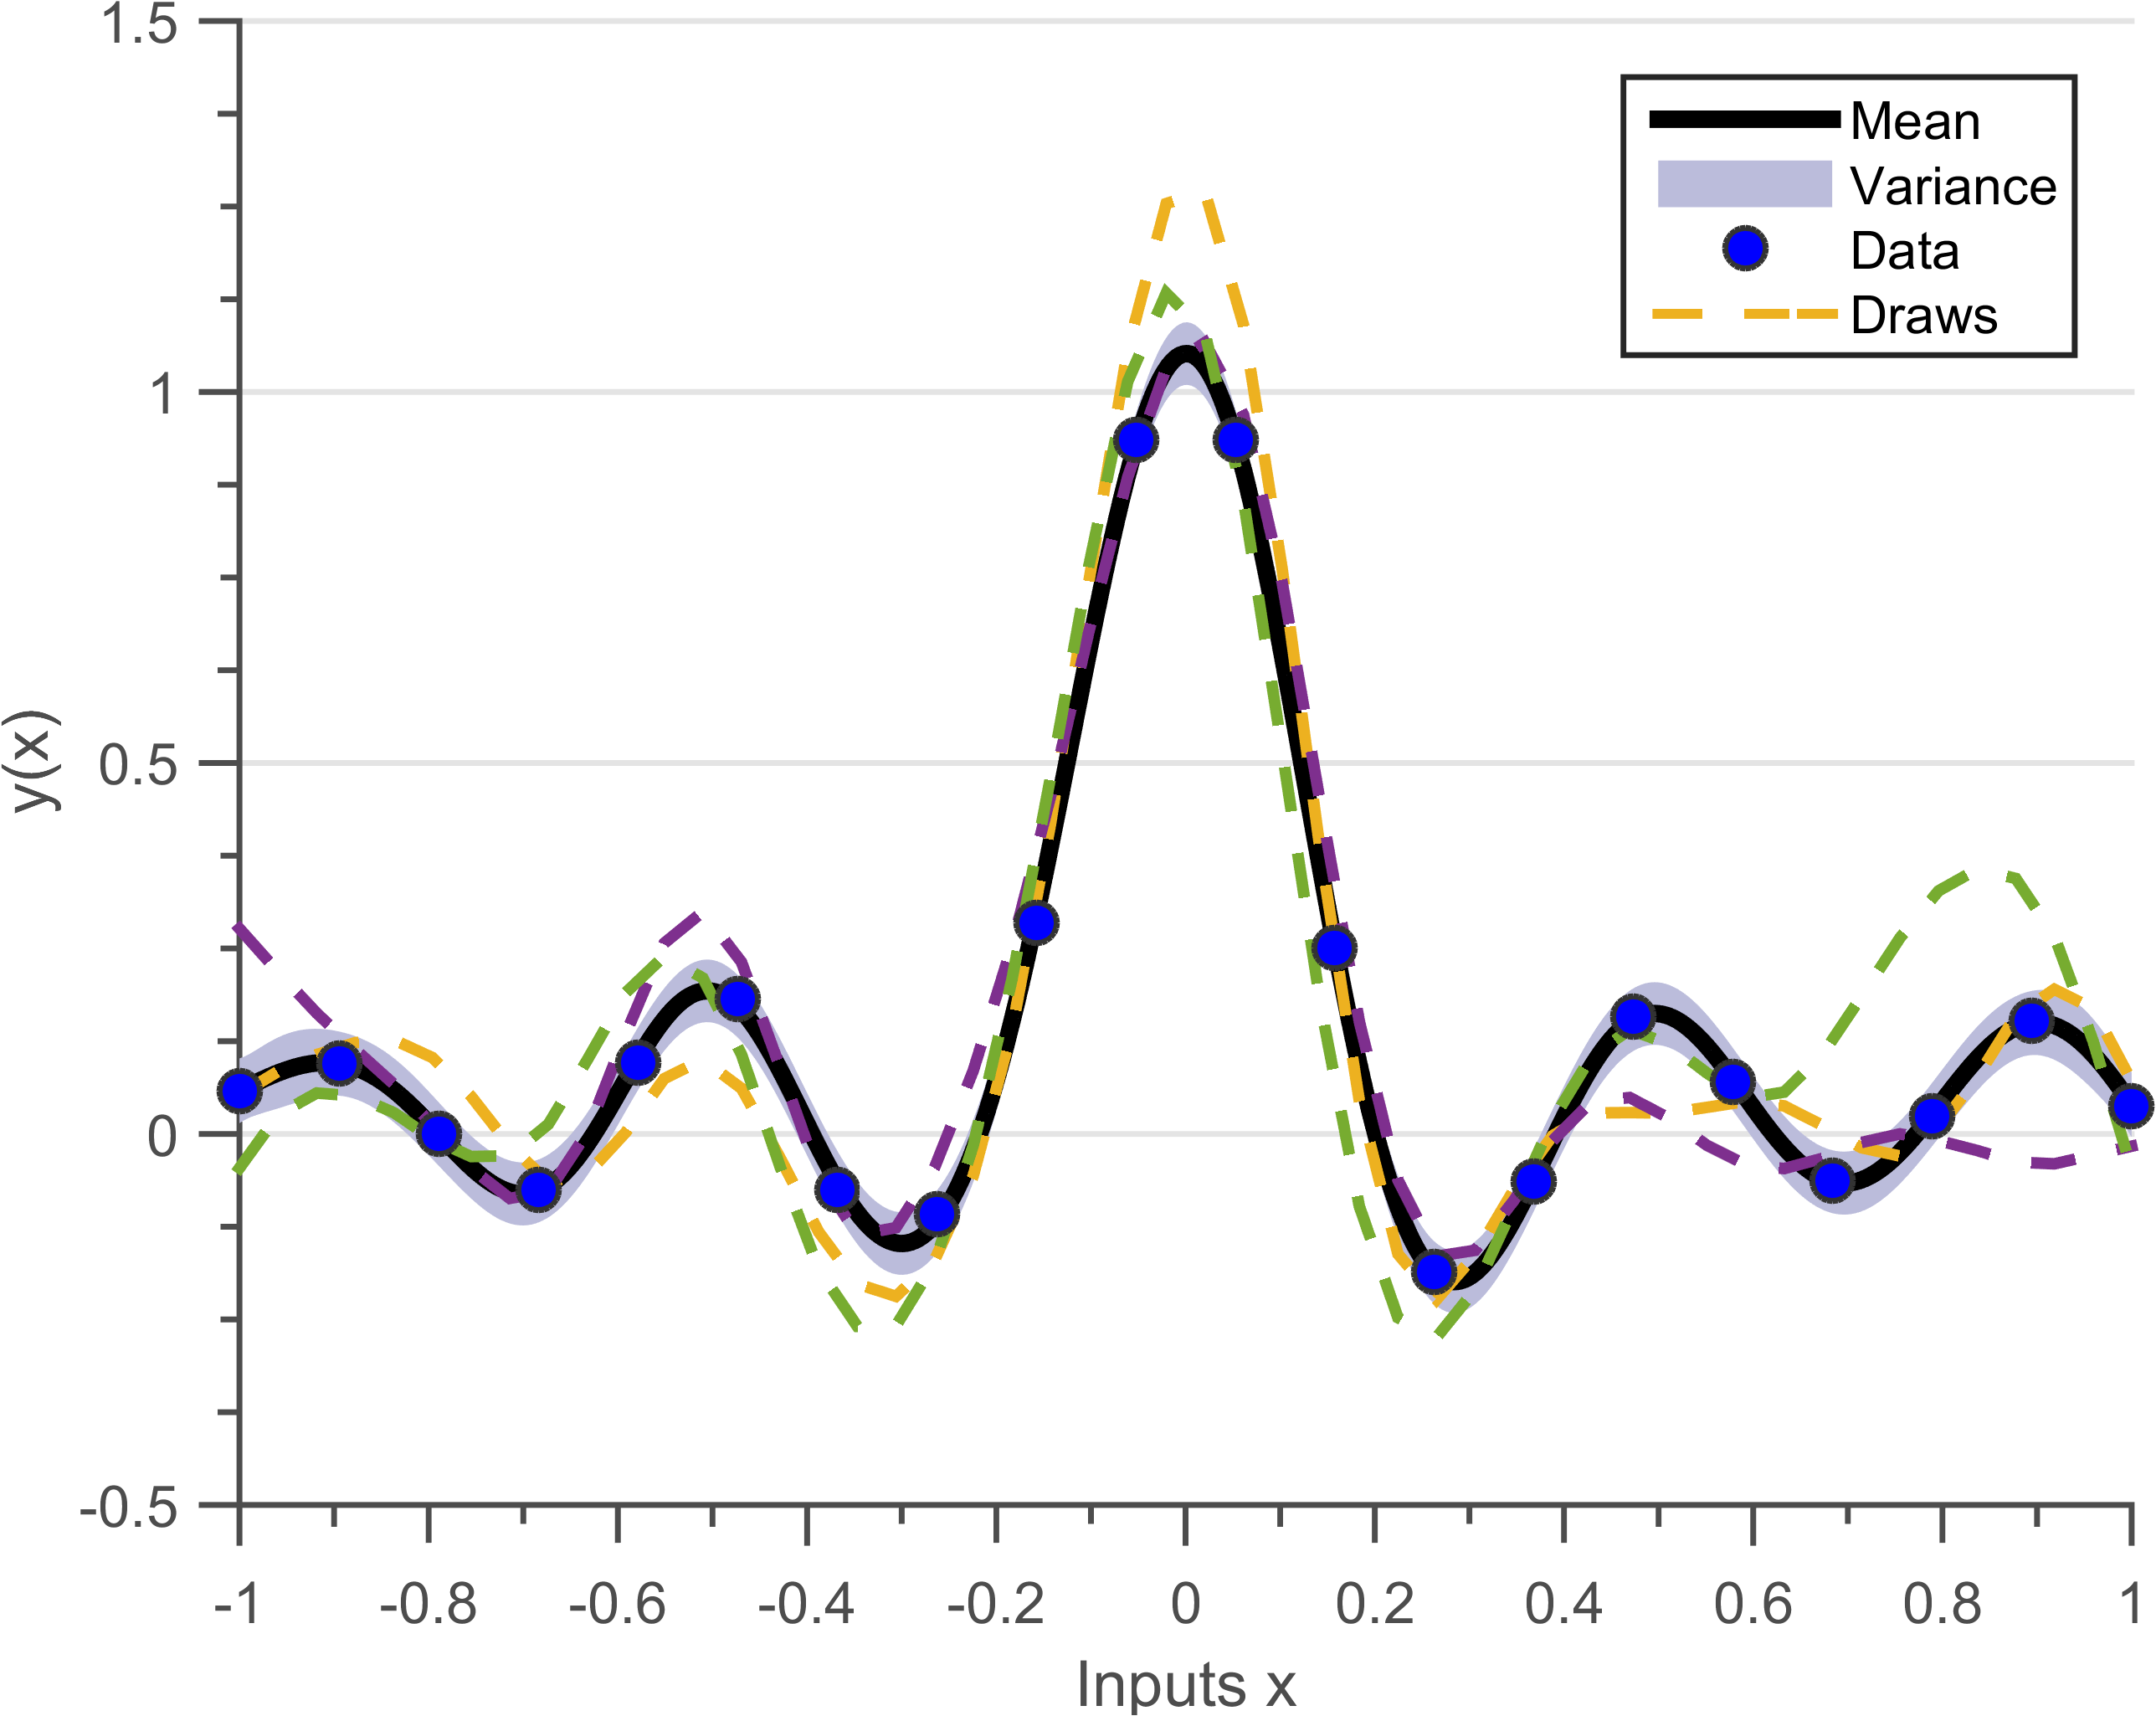
\includegraphics[width=0.29\textwidth]
        {images/part2/drawsOptimizedPosteriorSE}
        \label{subFigdrawsOptimizedPosteriorSE}
  }\quad
\caption{Posterior distributions from three different covariance functions after maximizing the hyper-parameters.}
       \label{figOptimizedPosteriorCh4}
\end{figure}

\marginnote{\textsl{Choosing functional form}}[1cm]
If nothing is known about the data or type of experiment, and the number of hyper-parameters are same, then the covariance function with the maximum optimized marginal likelihood should be preferred. By this logic the SE kernel should be the preferred functional form of the covariance for the data-set $\mathcal{D}_{2}$. If the number of hyper-parameters are not the same, then marginal likelihood tends to be higher for covariance functions with greater number of hyper-parameters. \cite{duvenaud-thesis-2014, lloyd2014automatic} propose to use the Bayesian Information Criterion (BIC)\footnote{The BIC again performs a trade-off between data-fit and model complexity, for more details refer to section \ref{subSecSMKernelApplication}} to choose optimal covariance functions if the number of hyper-parameters is different. 

\subsection{Spectral Mixture Kernels}\label{subSecSMKernel}
Spectral mixture kernels define a more general class of stationary kernels exploiting the Bochner's theorem \cite{bochner1959lectures}. They define the power spectrum ($S(s)$) as a scale location mixture of Gaussians \cite{wilson2013gaussian}. This has two benefits: firstly, with enough Gaussian components, scale location mixtures of Gaussians can approximate a curve up to arbitrary precision \cite{kostantinos2000gaussian, bishop2006pattern}, secondly, the inverse Fourier transform of a scale location mixture of Gaussians can be evaluated analytically and is also a mixture of Gaussians.

\begin{equation}\label{eqPowerSpectrumSSM}
    S_{SM}(s, \mu, \sigma, w) = \sum_{q=1}^{Q} \frac{w_{q}}{\sqrt{2\pi\sigma_{q}^2}}
\left ( \exp\left [ {-\frac{{(s-\mu_{q})^2}}{2\sigma_{q}^{2}}} \right ] + \exp\left [ {-\frac{{(-s-\mu_{q})^2}}{2\sigma_{q}^{2}}} \right ] \right  )
\end{equation}

Here, $ S_{SM}$ is the power spectrum of the spectral mixture kernel. Each Gaussian  component $q$ has a mean $\mu_{q}$, variance $\sigma_{q}$ and weight $w_{q}$ , there are total $Q$ such components. The second term $\exp\left [ {-\frac{{(-s-\mu_{q})^2}}{2\sigma_{q}^{2}}} \right ]$ is needed because a power spectrum of a valid kernels should be symmetric around $s=0$. The inverse Fourier transform of such a power spectrum will be a valid kernel and can be written as equation \ref{eqCovarianceKSM}. For a detailed derivation refer to \cite{wilson2014thesis}.

\begin{equation}\label{eqCovarianceKSM}
k_{SM}(d, \mu, \sigma, w) = \sum_{q=1}^{Q}w_{q}cos(2\pi\mu_{q}) exp[-2\pi^{2}d^{2}\sigma_{q}^2]
\end{equation}

Here, $k_{SM}$ is the covariance function of the above power spectrum (equation \ref{eqPowerSpectrumSSM}). The parameter $w_{q}$ is the weight of the Gaussian component $q$, the mean of the Gaussian component $\mu_{q}$ defines the period of kernel while the variance $\sigma_{q}$ of the Gaussian component denotes inverse of the length scale . 

\marginnote{\textsl{Pattern recognition}}[1cm]
\cite{wilson2014thesis} demonstrate that the spectral mixture kernels can be used as a replacement for many available kernels, since they define a general class of stationary kernels. Due to their expansive hypothesis space, they can be used as a means to perform automatic pattern discovery. Their Fourier transform can provide more understanding of the observation data-set (this is very similar to interpreting the Fourier transform of dynamic data) \cite{wilson2013gaussian}. One of the major hindrances of SE kernels is that they cannot be used for extrapolation, we cannot extrapolate an SE kernel a $\theta_{lengthScale}$ distance away from the last observation (figure \ref{figGPNoiseLessPosteriors}). Since Spectral mixture kernels can detect patterns in the data they can also be used to perform extrapolation\footnote{A detailed code can be found : \url{https://people.orie.cornell.edu/andrew/code/\#spectral}}. 

We propose to use this relationship between the covariance function and its Fourier transform to automatically identify parameters of a dynamic system. Dynamic engineering systems are generally parametrized by their modal frequencies and participation factors. In structural engineering, identification of modal frequencies is an important step for certification, while minor change in modal frequencies can help in fast discovery of failure. In the next section we apply the Spectral Mixture kernel to automatically identify the modal frequencies of a structural system, parts of the following work have been published in \cite{chiplunkar2017operational}.

\section{Application: Identifying Structural Dynamics Parameters}\label{subSecSMKernelApplication}
Modal analysis has been widely used as a means of identifying dynamic properties such as modal frequencies, damping ratios and mode shapes of a structural system. Traditionally, the system is subject to artificial input excitations and the output deformations (displacements, velocities or accelerations) are measured. These later help in identifying the modal parameters of the system, this process is called Experimental Modal Analysis (EMA). 

\marginnote{\textsl{OMA}}[1cm]
Since the last decade Operational Modal Analysis (OMA) has gained considerable interest in the structural dynamics community. OMA identifies the modal parameters only from the output measurements while assuming ambient excitations as random noise. OMA is cheaper because it does not require expensive experimental setup and can be used in real time operational use cases such as health monitoring \cite{peeters2005industrial, shahdin2010correlating, rainieri2007automated}. 

\marginnote{\textsl{MDOF}}[1cm]
In the last few decades several algorithms primarily using the assumption of second order differential, Multi Degree Of Freedom (MDOF) system (equation \ref{eq:secondOrderSystem}) have been developed to find the modal parameters \cite{guillaume2003poly, richardson1982parameter}.

\begin{equation}\label{eq:secondOrderSystem}
    \myMatrix{M}\{\ddot{x}(t)\} + \myMatrix{C}\{\dot{x}(t)\} + \myMatrix{K_{stiffness}}\{x(t)\} = \{\VEC{f}(t)\}
\end{equation}

Here, $\myMatrix{M}$, $\myMatrix{C}$ and $\myMatrix{K}$ denote the mass, damping and stiffness matrices respectively. $\{x(t)\}$ and $\{\VEC{f}(t)\}$ denote the displacement and force vectors at the time $t$, while $\ddot{x}(t)$ and $\dot{x}(t)$ denote the second and first time derivative of displacement respectively. Figure \ref{subfig:randomOutput} shows an example of ambient measurements $x(t)$ on a structure.  In almost all OMA algorithms the measurement $x(t)$ is assumed to be generated from a random force excitation. 

\paragraph{Earlier Work}
The Natural Excitation Technique (NExT) \cite{james1995natural} proves that the auto-correlation function $k(\tau)$ can be written as sum of decaying sinusoid's \cite{spitznogle1970representation, ibrahim1977method, guillaume2003poly}. The auto-correlation describes the similarity between measurement as a function of time lag $\tau$ between them (figure \ref{subfig:autocorrelationOutput}).  
\marginnote{\textsl{NExT}}[-1cm]

\begin{equation}\label{eq:NeXT}
    k(\tau) = \int x(t)x(t-\tau)dt \quad k(\tau) = \sum A_{i}exp(-\lambda_{i}\tau)sin(B_{i}\tau)
\end{equation}

Here, $k(\tau)$ denotes the auto-correlation for random vector $x(t)$ as a function of time lag $\tau$. While, $\lambda_{i}$ and $A_{i}$ denote the modal frequency and mode shapes for the $i^{th}$ mode. The above coefficients are found by minimizing the least square error between the measured $k(\tau)$ and the predicted $k(\tau)$ from equation \ref{eq:NeXT}.

\marginnote{\textsl{RFP}}[1cm]
If we assume the measurement $x(t)$ to be a stationary random process, then according to Bochner's theorem, the Fourier transform of $k(\tau)$ (power spectrum $S(s)$) exists \cite{bochner2016lectures}. Figure \ref{subfig:psdOutput} shows the power spectrum calculated for the measurement $x(t)$ shown in figure \ref{subfig:randomOutput}. Using the above mentioned second order differential assumption a Rational Fractional Polynomial (RFP) (equation \ref{eq:RFP}) can be used to fit a power spectrum \cite{richardson1982parameter, allemang1998unified, chauhan2007unified}.

\begin{equation}\label{eq:RFP}
S(s) = \int k(\tau) e^{-2 \pi is^{T} s}d\tau \quad    S(s) = \frac{\sum a_{k}(s)^{k}}{\sum b_{l}(s)^{l}}
\end{equation}

Here, the poles of the polynomial denote the modal frequencies, while other modal parameters can be derived from the coefficients $a_{k}$ and $b_{l}$. The coefficients of the polynomial can be found by minimizing the least squared error. RFP based algorithms face problems of numerical stability a value of number of modes ($l$) increases.

\begin{figure*}[!ht]
  \centering
  \subfigure[Measured output on accelerometers $x(t)$]
  {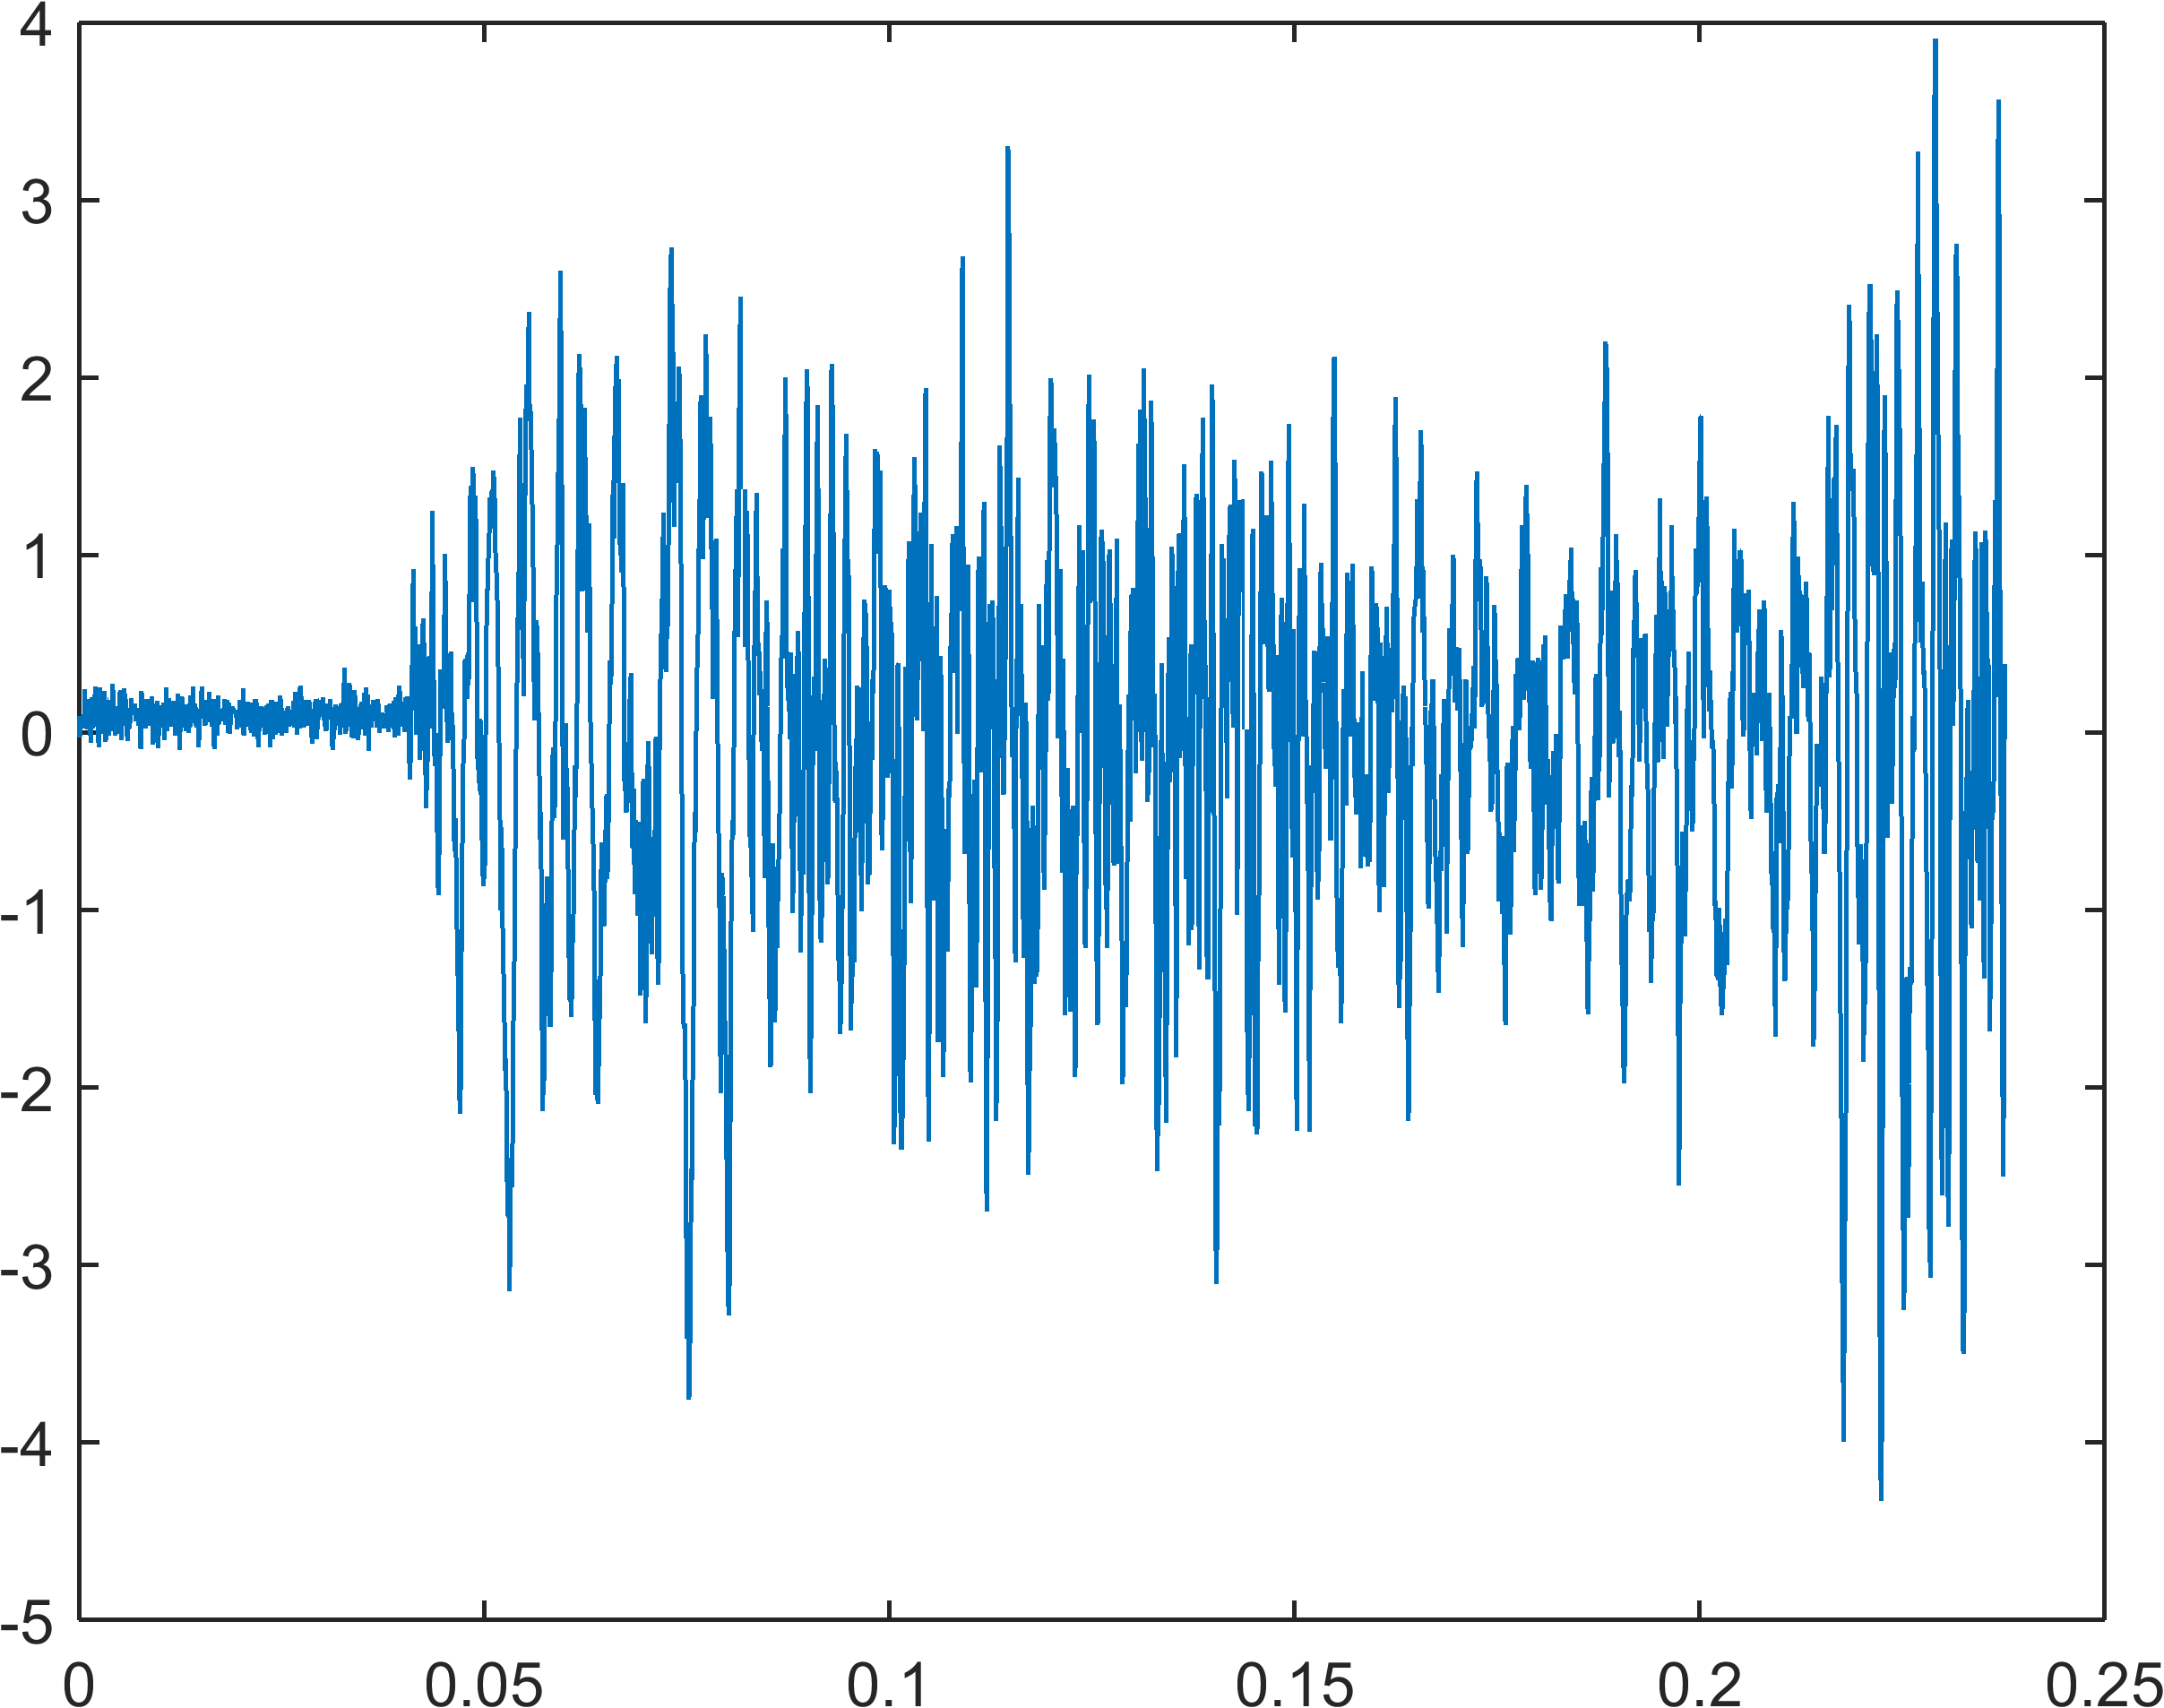
\includegraphics[width=0.3\textwidth]{images/part2/randomOutput}\label{subfig:randomOutput}}\quad
  \subfigure[Auto-correlation $k(\tau)$ of the measured output fig: \ref{subfig:randomOutput}]
  {\includegraphics[width=0.3\textwidth]{images/part2/autocorrelationOutput}\label{subfig:autocorrelationOutput}}\quad
  \subfigure[Power spectrum density $S(s)$ of the output fig: \ref{subfig:randomOutput}]
  {\includegraphics[width=0.3\textwidth]{images/part2/psdOutput}\label{subfig:psdOutput}}
  
  \caption{Different types of measurements for estimation of Modal parameters in OMA}
\end{figure*}

\renewcommand{\arraystretch}{1.2}
\begin{table}[!ht]
    \centering
\begin{tabularx}{\textwidth}{c|c|c}
  \hline
  Measurement & Auto-correlation & Power Spectrum \\
  \hline
  $x(t)$ & $k(\tau) = \int x(t)x(t-\tau)dt$ &  $S(s) = \int k(\tau)exp(-2 \pi i s^{T} \tau )d\tau$\\
  \hline \hline
  \multicolumn{3}{|c|}{Assumption: Second Order Differential}\\
  \hline
   & $ \sum A_{i}exp(-\lambda_{i}\tau)sin(B_{i}\tau)$ & $\frac{\sum a_{k}(s)^{k}}{\sum b_{l}(s)^{l}}$\\
   \hline \hline
   \multicolumn{3}{|c|}{Assumption: Gaussian Mixture Model}\\
   \hline
   $GP(0 , k_{SM})$ 
   & $  \sum w_{i} cos(2\pi\mu_{i}\tau) exp\{-2\pi^{2}\sigma_{i}^{2}\tau^{2}\}$ 
   & $ \sum w_{i}  \frac{1}{\sqrt{2\pi\sigma_{i}^{2}}}exp\{\frac{1}{2\sigma_{i}^{2}}(s-\mu_{i})^{2}\} $\\
   \hline
\end{tabularx}
\caption{Comparison of fitting functions}
  \label{tab:comparisonOfFittingFunctions}
\end{table}

\begin{mdframed}[hidealllines=true,backgroundcolor=blue!20]
\paragraph{Contribution}
The above mentioned OMA algorithms NExT in the time lag ($ \tau$) domain and RFP in the frequency domain ($s$), assume the dynamic behaviour to be a second order differential system. This assumption fails for non-linear systems and for cases where modal frequencies are very close. Instead we propose to use the spectral mixture kernel to fit the measurement $x(t)$. 

Using the same hypothesis used in section \ref{subSecSMKernel}, we can say that a scale-location mixture of Gaussian components can approximate any distribution. We thus place a scale-location mixture of Gaussians on the power spectrum ($S(s)$), this means that we are assuming a prior distribution of $x(t)$ as a GP with a Spectral Mixture kernel (equation \ref{eqTimeFitting}). The hyper-parameters of the system are: the mean $\mu_{q}$ defines the modal frequency, the variance $\sigma_{q}$ which is a measure of damping, the weight $w_{q}$ which defines the participation factor of component $q$ and the total number of components $Q$.

\begin{equation}\label{eqTimeFitting}
\Pr[x(t)] = GP(0, k_{SM} = \sum_{q=1}^{Q}w_{q}cos(2\pi\mu_{q}) exp[-2\pi^{2}\tau^{2}\sigma_{q}^2)
\end{equation}

\marginnote{\textsl{Table \ref{tab:comparisonOfFittingFunctions}}}[1cm]
\sloppy We would like to emphasize that keeping the computational complexities aside, fitting a Spectral Mixture GP in time-domain (equation \ref{eqTimeFitting}), fitting spectral mixture (equation \ref{eqCovarianceKSM}) on covariance values and fitting a scale-location mixture of Gaussians (equation \ref{eqPowerSpectrumSSM}) on the power spectrum are equivalent. In the publication \cite{chiplunkar2017operational} we fit a scale-location mixture of Gaussians on the power spectrum, here we propose to fit the GP on the measurements $x(t)$ . Refer to table \ref{tab:comparisonOfFittingFunctions} for a more comprehensive view at various fitting functions.

\marginnote{\textsl{Choosing $Q$}}[1cm]
While the modal parameters can be chosen by minimizing the least square error, how to choose the number of modes is a recurring question in several OMA algorithms. This problem is partially resolved by using stabilization diagrams or mode identification functions \cite{allemang1998unified, williams1985multivariate, shih1988complex}. But in practical situations, engineering judgment is often required to estimate the optimal modal order. To automatically choose $Q$, we use the Bayesian Information Criteria (BIC) \cite{findley1991counterexamples} which penalizes more complex models to estimate the parameter $Q$. The BIC estimate has been earlier used to find the optimal functional form of covariance function \cite{duvenaud2013structure}

\begin{equation}\label{eq:BIC}
    BIC(Q) = N\ln(ML) + N_{hyp}\ln(N)
\end{equation}

\marginnote{\textsl{BIC}}[1cm]
Here, $n$ denotes the number of data-points to fit, $ML$ denotes the marginal likelihood of the fit and $N_{hyp}$ denote the number of hyper-parameters to fit. The BIC performs a trade-off between the data-fit term $N\ln(ML)$ and the complexity penalty term $N_{hyp}\ln(N)$, basically penalizing for over-fitting. Lowest value of BIC is preferred. 
\end{mdframed}

Generally, identification of modal frequencies requires engineering judgment, i.e. engineers have to look at the stabilization diagrams and figure out the optimal value of modal order. Using the Spectral mixture kernel we have encoded the knowledge of peaks in the power spectrum which in combination with BIC has eliminated the need to perform costly engineering judgment exercises and has made the process automatic. We now compare the accuracy of finding modal frequencies using a spectral mixture kernel vs NExT \cite{james1995natural} methodology for a toy data-set, and then later for a real data-set of HCC building \cite{brincker2000modal}.

\subsection{Results on a toy data-set}
In this section we conduct experiments, applying our approach on a highly damped 3 degree of freedom system. As stated earlier we fit a GP model having a spectral mixture covariance on the measurements $x(t)$ for varying number of Gaussian components $Q$. We then evaluate the BIC to find the optimal value of $Q$ for this measurement. The results of automatic identification are then compared to that of NeXT identification method. 

All experiments were performed on an Intel quad-core processor with 4Gb RAM. The Spectral Mixture technique suffers from multiple minimas and thus care should be taken while initializing the hyper-parameters\footnote{For fast optimization we first fit a Gaussian Mixture model on the power spectrum to initialize the hyper-parameters and then optimize the marginal likelihood.}.  

Table \ref{tabComparisonOfModalFrequenciesToyData} shows the comparison of frequencies for Modal frequencies predicted using NeXT algorithm and Spectral Mixture algorithm. We can observe that the NeXT method cannot predict the third frequency with enough accuracy. This is because the third frequency has the hignest value of damping.

\renewcommand{\arraystretch}{1}
\begin{table}[!ht]
    \centering
\begin{tabular}{|l|l|l|l|}
  \hline
   & Real Frequency & Error NeXT Frequency & Error Spectral Mixture\\
  \hline 
  \hline
First Frequency (Hz) & 17.5 & 2.7 \% & 0.28 \%\\
Second Frequency (Hz)  & 30 & 3.4 \% & 4.1 \%\\
Third Frequency (Hz) & 35 & 12.34\% & 5.1\%\\
   \hline
\end{tabular}
\caption{Comparison of Modal frequencies for toy data-set}
  \label{tabComparisonOfModalFrequenciesToyData}
\end{table}

Figure \ref{subfig:stabilizationDiagram} shows the stabilization diagram with increasing number of Gaussians $Q$. As we progressively increase the number of components we start getting more and more modal frequencies. We call a frequency stabilized if the difference between modal frequencies of two subsequent $Q$ is less than $1\%$. The green points are stabilized frequencies. Figure \ref{subfig:bicVsQ} shows the BIC criterion with increasing number of Gaussian's $Q$. We can see that that the BIC is minimum for $Q=6$ and hence if we add any more Gaussians for our data-set we will be over-fitting. The red line in figure \ref{subfig:stabilizationDiagram} shows the $Q$ with minimum BIC and hence the stabilized frequencies for this automatically become our modal frequency predictions.

\begin{figure*}[!ht]
  \centering
  \subfigure[Stabilization diagram with increasing number of Gaussians $Q$, the dots denote the stabilized frequencies. We can observe that as the number of $Q$ increases the algorithm starts finding better and better modes.]
  {\includegraphics[width=0.45\textwidth]{images/part2/stabilizationDiagram_toyData}\label{subfig:stabilizationDiagram}}\quad
    \subfigure[The BIC criterion with increasing number of Gaussian's $Q$. We can see that that the BIC is minimum for $Q=6$ and hence if we add anymore Gaussian's for our data-set we will be performing over-fitting]
  {\includegraphics[width=0.45\textwidth]{images/part2/bicVsQ}\label{subfig:bicVsQ}}\quad
  
  \caption{Results of spectral mixture kernels on a toy data-set}
\end{figure*}

\subsection{Results on a HCT building data-set}
We now apply our methodology on real ambient response of Heritage Court Tower (HCT) Building\footnote{The data is available at : http://www.brinckerdynamics.com/oma-toolbox}. The responses are measured at 6 different points on the building resulting in 6 different power spectrums. We compare the modal frequencies obtained using Spectral Mixture kernel with the modal frequencies obtained in the original paper \cite{brincker2000modal}. To compare the performance we automatically identify modal frequencies present in each of the 6 power spectrums and take the mean of the stabilized frequencies.

Table \ref{tabComparisonOfModalFrequenciesToyData} shows the comparison of Modal frequencies predicted in \cite{brincker2000modal} with the Spectral Mixture algorithm. The results of the two methods are very similar, although the frequencies obtained by spectral mixture GP are completely automatic. 

\renewcommand{\arraystretch}{1}
\begin{table}[!ht]
    \centering
\begin{tabular}{|l|l|l|}
  \hline
    & Spectral Mixture & \cite{brincker2000modal} \\
  \hline 
  \hline
First Frequency (Hz) & 1.23 & 1.23\\
Second Frequency (Hz)  & 1.29 & 1.27\\
Third Frequency (Hz) & 1.43 & 1.45\\
Fourth Frequency (Hz) & 3.87 & 3.86\\
Fifth Frequency (Hz) & 4.28 & 4.25\\
   \hline
\end{tabular}
\caption{Comparison of Modal frequencies for HTC data-set}
  \label{tabComparisonOfModalFrequenciesHTCData}
\end{table}

\begin{figure*}[!ht]
  \centering
  \subfigure[Stabilization diagram for one of the 6 power spectrums. The green dots denote the stabilized frequencies, the red line denotes minimum BIC. We can observe that as the number of $Q$ increases the algorithm starts finding better and better modes.]
  {\includegraphics[width=0.45\textwidth]{images/part2/stabilizationDiagram_HTCBuildingData}\label{subfigStablizationHTCData}}\quad
    \subfigure[The BIC criterion with increasing number of Gaussian's $Q$. We can see that that the BIC is minimum for $Q=8$ and hence if we add anymore Gaussian's for our data-set we will be performing over-fitting]
  {\includegraphics[width=0.45\textwidth]{images/part2/bicVsQ_HTCBuilding}\label{subfigBICHTC}}\quad
  
  \caption{Results of spectral mixture kernels on real data from HTC building}
\end{figure*}

Figure \ref{subfigStablizationHTCData} shows the stabilization diagram with increasing number of Gaussians $Q$. We can observe that as the number of $Q$ increases the algorithm starts finding better and better modes, three modes start stabilizing from $Q=5$. Figure \ref{subfigBICHTC} shows the BIC criterion with increasing number of Gaussian's $Q$. We can see that that the BIC is minimum for $Q=8$ and hence if we add any more Gaussians for our data-set we will be  over-fitting. 

In the current setting of the Spectral Mixture model we propose an automatic way to identify the most important frequencies of a structural system. Neither the mode shapes nor the damping ratios are estimated in the current format. In the future we would like to derive a method to estimate mode-shape and damping ratio such that the contributions of neighbouring Gaussians are also taken into account. 

\section{Summary and discussion}
This chapter discussed only a small number of possible covariance functions, table \ref{tabListOfCovarianceFUnctions} provides a list of basic covariance functions that we have encountered thus far. Several other other functional forms of the covariance function exist in the literature, for example Gibbs kernel, Rational Quadratic kernel, Periodic kernel etc for more detailed list please refer to works of \cite{Rasmussen2005, duvenaud2013structure, wilson2014thesis}. . 

%\renewcommand{\arraystretch}{1}
\begin{table}[!ht]
    \centering
\begin{tabularx}{\textwidth}{|l|l|X|}
  \hline
Kernel Name  & Expression $k(x_{i}, x_{j})$ & Constituent functions \\
  \hline 
  \hline
Constant & \small $\sigma_{c}^2$ & Constant functions \normalsize\\
  \hline 
Noise & \small $\sigma_{n}^2\delta_{x_{i}x_{j}}$ & White noise \normalsize\\
  \hline 
Linear & \small $\phi(x_{i})\Sigma\phi(x_{j})$ & Linear combination of $\phi$ \normalsize\\
  \hline 
Neural Network & \small $\theta_{1}^{2}\frac{2}{\pi} sin^{-1}\left ( \frac{2x\theta_{2}x'}{\sqrt{(1+2x^{T}\theta_{2}x)(1+2x'^{T}\theta_{2}x')}} \right )$ & Linear combinations of Sigmoids \normalsize\\
  \hline 
Standard Exponential & \small $\theta_{amplitude}^2exp[-\frac{\tau^2}{2\theta_{lengthScale}^2}]$ & Infinitely Differentiable functions \normalsize\\ 
  \hline 
Mat\'ern & \small $\theta_{amplitude}^2\frac{2^{1- \nu }}{\Gamma (\nu)}\left ( \frac{\sqrt{2\nu(\tau))}}{\theta_{lengthScale}} \right )^{\nu}K_{\nu}\left ( \frac{\sqrt{2\nu(\tau))}}{\theta_{lengthScale}} \right)$ & Adjustable differentiability \normalsize\\
  \hline 
Spectral Mixture & \small  $\sum_{q=1}^{Q}w_{q}cos(2\pi\mu_{q}) exp[-2\pi^{2}\tau^{2}\sigma_{q}^2]$ & Summation of periodic kernels \normalsize\\
   \hline
\end{tabularx}
  \label{tabListOfCovarianceFUnctions}
  \caption{List of covariance functions}
  \end{table}
  
We start off this chapter by defining a few important properties (section \ref{secPropertiesOfCovariance}) of the covariance functions. Section \ref{secNonStationaryKernels} details a few non-stationary kernels and discusses how Bayesian Linear Regression can be effectively seen as a GP regression with linear covariance function. Section \ref{secStationaryKernels} describes stationary kernels, Using the Bochner's theorem we can effectively represent a stationary kernel into its Fourier transform, this gives rise to more interpretation of the constituent family of functions. Section \ref{subsecCH4Experiments} demonstrates the effects on posterior prediction for different functional forms of covariance functions. For each covariance function we try to give a visualization of the shape of constituent functions by randomly drawing functions from their priors. 

\marginnote{\textsl{Modal parameter estimation}}[1cm]
The main contribution of this chapter is demonstration on how to use GP regression to automatically detect modal parameters of structural dynamics. To the best of our knowledge, such a method has not been used in the earlier literature to identify modal parameters. Using the spectral mixture kernels we demonstrate how to build models for structural dynamic experiments and automatically identify dynamic parameters such as modal frequency. This is a very early stage of application of Spectral Mixture Kernel for system identification, and there remain problems such as identification of mode-shape, and damping ratio in this algorithm. We wish to tackle these problems in the future. 

As mentioned earlier the core aim of machine learning was to identify patterns and extrapolate on data automatically. There are two main approaches in pattern discovery for GPs; one is based on increasing the hypothesis space by defining a process over all stationary kernels \cite{wilson2012process}. The second which defines a language of kernels and iteratively adds basic kernels to come up with an explanation to the pattern in the data \cite{lloyd2014automatic}. In the next chapter we will look in detail at how to build more complex kernels using basic kernels. Which approach will be retained in the long term is difficult to predict to say but research in automatic pattern detection is a highly active subject. 

%%% Local Variables: 
%%% mode: latex
%%% TeX-master: "isae-report-template"
%%% End: 


\chapter{Combining Basic Covariance Functions}
\label{chapCombiningBasicCovariances}

\begin{mdframed}[hidealllines=true,backgroundcolor=lightgray!20]
\section*{Résumé}
Souvent, le type d'information initiale que nous voulons intégrer n'est pas disponible sous la forme de fonctions de covariance basiques. Heureusement, plusieurs nouveaux noyaux peuvent être créés en fusionnant les noyaux de base que nous avons vus dans le chapitre précédent. Ce chapitre est inspiré par les travaux aux  \cite{bishop2006pattern, mackay2003information, durrande2001etude, durrande2013anova}.


La section \ref{secSingleDimension} décrit comment combiner les noyaux pour créer des noyaux unidimensionnels. Nous fournissons une explication intuitive de ce qui se produit lorsque nous ajoutons ou multiplions des noyaux, ces types de noyaux peuvent être utilisés pour détecter et séparer les modèles de données. La section \ref{subsubsecCh4ApplicationCP} décrit comment créer des noyaux pour des dimensions plus élevées. Ce type de noyaux peut être utilisé pour effectuer une analyse de sensibilité ou intégrer une structure à dimension réduit en taille dans les données.

Dans ce chapitre, nous utilisons une combinaison de noyaux de base pour identifier l'apparition de non linéairités dans les systèmes physiques. Par exemple, nous identifions l'initiation de la séparation de l'écoulement pour le profil
(d'aile) NACA 0012 et l'initiation de la plasticité pour l'alliage AL6061 en utilisant un critère statistique pour la détection automatique de la non-linéarité (section \ref{subsubsecCh4ApplicationCP}) \cite{chiplunkar:hal-01555401}. Nous construisons enfin un modèle de GP pour prédire la position du choc aérodynamique en régime transsonique (section \ref{subecInterpolationOfAerodynamicPressures}) \cite{oatao18004}.
\end{mdframed}


%\pagebreak

\section{Introduction}

What if the kind of patterns that we wish to encode are not possible by using the basic kernels described in chapter \ref{chapBasicCovarianceKernels}? What if we wish to encode several different patterns in our hypothesis space? Or what if we want to build models for data sets with more than one input dimension? Thankfully, many new kernels can be constructed by merging a few basic kernels, in this chapter we answer the above questions. 

The original contribution of this chapter is to apply the newly created covariance functions to create engineering design models. The set of equations below are a few simple methods to create valid covariance functions \cite{bishop2006pattern, mackay2003information, durrande2001etude, durrande2013anova}. 

\begin{align}
k(x_{1}, x_{2}) =  & k_{1}(x_{1}, x_{2}) + k_{2}(x_{1}, x_{2})  \label{eqCh5AddingCovariances} \\
k(x_{1}, x_{2}) =  & k_{1}(x_{1}, x_{2}) \times k_{2}(x_{1}, x_{2}) \label{eqCh5MultiplyingCovariances} \\
k(x_{1}, x_{2}) =  & q(x_{1})k_{1}(x_{1}, x_{2})q(x_{2}) \label{eqCh5MultiplyingWithFunction} \\
k(x_{1}, x_{2}) =  & k_{1}(h(x_{1}), h(x_{2})) \label{eqCh5ComposedCovariances} \\
k(x_{1}, x_{2}) =  & g(g(k_{1}(x_{1}, x_{2}), x_{1}), x_{2} ) \label{eqCh5LinearOperatorCovariances} \\
k(x_{1}, x_{2}) = & \int k_{1}(x_{1}, u)k_{2}(u, x_{2})du \label{eqConvolutionProcess}
\end{align}


Here, $k_{1}(x_{1}, x_{2})$ and $k_{2}(x_{1}, x_{2})$ are valid covariance function, while $q(x)$ and $h(x)$ are any continuous functions. Equation \ref{eqConvolutionProcess} defines a covariance function through convolution of two kernels, while equation \ref{eqCh5LinearOperatorCovariances} defines transformation through a linear operator $g\left ( . \right ) \in \mathcal{C}^{2}$, for more discussion on this equation refer to chapter \ref{chapAddingEquationsInGP}. 

Let us take the case of a 2-dimensional input vector\footnote{The superscript is used to number of dimension and does not denote the power.} $\VEC{x}$ such that $\VEC{x} = \{x^{1}, x^{2}\}$ ($x^{1}$, $x^{2}$ are coordinates of $\VEC{x}$ in the first and second dimension respectively). Then the following covariance functions are also valid.

\begin{align}
k(\VEC{x_{1}}, \VEC{x_{2}}) = k_{1}(x_{1}^{1}, x_{2}^{1}) + k_{2}(x_{1}^{2}, x_{2}^{2}) \label{eqCh5AddingAcrossDimensionsCovariances} \\
k(\VEC{x_{1}}, \VEC{x_{2}}) = k_{1}(x_{1}^{1}, x_{2}^{1}) \times k_{2}(x_{1}^{2}, x_{2}^{2}) \label{eqCh5MultiplyingAcrossDimensionsCovariances} 
\end{align}

The current chapter is written to provide intuition on what happens when we combine covariance functions. This chapter unfolds as follows; section \ref{secSingleDimension} provides intuition on combining kernels for one-dimensional inputs, while section \ref{secMultiDimensionalKernels} details how to create covariance functions for higher-dimensions (equation \ref{eqCh5AddingAcrossDimensionsCovariances} and \ref{eqCh5MultiplyingAcrossDimensionsCovariances}) inputs. 

\section{One dimensional inputs}\label{secSingleDimension}
Combining kernels can give rise to interesting features, in this section we provide intuition on combining kernels in one dimension. Section \ref{subsecStructureKernelsMultiplyingKernels} details effects of multiplying kernels (equation \ref{eqCh5MultiplyingCovariances}) while section \ref{subsecStructureKernelsAddingKernels} describes effects of adding kernels (equation \ref{eqCh5AddingCovariances}). Section \ref{subsubsecCh4ApplicationCP} describes the Change-Point (CP) kernel. We use the CP kernel to detect start of plasticity in elastic structures such as beams and start of flow separation on an airfoil \cite{chiplunkar:hal-01555401}. 


\subsection{Multiplying Kernels} \label{subsecStructureKernelsMultiplyingKernels}
Multiplying two covariance functions acts as an AND operator, the resulting kernel has high value only if we have high value on both the kernels. Multiplying a Linear kernel $T$ times, will result in a $T^{th}$ order polynomial regression (equation \ref{eqCh4PolynomialCovariance}). 

\begin{equation}\label{eqCh4PolynomialCovariance}
k_{Lin} = w_{0} + w_{1}x_{1}^T x_{2} \quad k_{Poly} = \prod_{i=1}^{T} \left (w_{0}^{i} + w_{1}^{i}x_{1}^T x_{2} \right)
\end{equation}

Equation \ref{eqMultiLinSECovariance} shows the prior obtained after multiplying a Linear and a SE kernel. This covariance function resembles a SE covariance function but with the amplitude hyper-parameter ($\theta_{amplitude} = \textcolor{red}{x_{1}x_{2}}$) proportional to the  distance. 

\begin{equation}\label{eqMultiLinSECovariance}
k_{Multi} = \textcolor{red}{x_{1}x_{2}} exp[- \frac{\tau^2}{2}]
\end{equation}

Figure \ref{subFigPriorMultiLinSE} shows random draws obtained using $k_{Multi}$ covariance,  the hyper-parameters of the linear kernel are $w_{0}=0$ and $w_{1}=1$, this means that there is no intercept and $k_{Lin}(x_{1}, x_{2}) = x_{1}x_{2}$. The hyper-parameters of the SE part are $\theta_{amplitude}=1$ and $\theta_{lengthScale}=1$, similar to figure \ref{subFigpriorDrawsSE}. Since multiplying two kernels is an AND operation, $k_{Multi}$ tends to zero at $x=0$ since $k_{Lin}$ is zero at $x=0$. 

\begin{figure}[!ht]
  \centering
    \subfigure[{Draws from a GP prior with mean zero and kernel obtained by \textbf{multiplying} a Linear kernel with SE kernel. The hyper-parameters of the linear kernel are $w_{0}=0$ and $w_{1}=1$ while the hyper-parameters of the SE part are $\theta_{amplitude}=1$ and $\theta_{lengthScale}=1$. We see that the variance at $x=0$ goes to zero, since multiplication is an AND operation}]
  {
        \includegraphics[width=0.45\textwidth]
        {images/part2/drawsMultiLinSE}
        \label{subFigPriorMultiLinSE}
  }\quad
\subfigure[{Draws from a GP prior with mean zero and kernel obtained by \textbf{adding} a Linear kernel with SE kernel. The hyper-parameters of the linear kernel are $w_{0}=0$ and $w_{1}=1$ while the hyper-parameters of the SE part are $\theta_{amplitude}=1$ and $\theta_{lengthScale}=1$. We see that the variance at $x=0$ goes to variance of SE kernel, since multiplication is an OR operation}]
  {
        \includegraphics[width=0.45\textwidth]
        {images/part2/drawsSumLinSE}
        \label{subFigPriorAddLinSE}
  }\quad

       \caption{Random draws from combining a Linear and SE kernel. The solid black line defines the mean function, shaded blue region defines 95\% confidence interval (2$\sigma$) distance away from the mean. The dashed lines represent five functions drawn at random from a GP prior. Random functions drawn from a linear GP are linear.}
       \label{figPrior}
\end{figure}


\subsection{Adding Kernels} \label{subsecStructureKernelsAddingKernels}
Adding two kernels acts as an OR operator, this means that the resulting kernel will have high value if either of the two kernels have high value \cite{durrande2011additive}. 

Figure \ref{subFigPriorAddLinSE} shows the prior obtained after adding a Linear and a SE kernel. The hyper-parameters of the linear kernel are $w_{0}=0$ and $w_{1}=1$, this means that there is no intercept and $k_{Lin}(x_{1}, x_{2}) = x_{1}^Tx_{2}$. The hyper-parameters of the SE part are $\theta_{amplitude}=1$ and $\theta_{lengthScale}=1$, similar to figure \ref{subFigpriorDrawsSE}. 

The Linear kernel discussed in section \ref{subSecCh4LinearKernel} is a sum of three covariance functions; a constant covariance ($\textcolor{red}{w_{0}}$), a linear covariance ($\textcolor{blue}{w_{1}x_{1}x_{2}}$) and a white noise covariance function ($\textcolor{green}{\sigma_{n}^2\delta_{xx'}}$) (equation \ref{eqDistributionOfLinearKernel}). Similarly, the noisy posterior case discussed in section \ref{figGPNoiseLessPosteriors} is a case of adding a SE kernel with a white noise kernel, a heteroscedastic\footnote{Noise depending on the inputs} noise model can be similarly created by adding several kernels together.

\begin{equation}\label{eqDistributionOfLinearKernel}
k(x_{1}, x_{2}) = \textcolor{red}{w_{0}} + \textcolor{blue}{w_{1} x_{1}^T x_{2}} + \textcolor{green}{\sigma_{n}^2\delta_{xx'}}
\end{equation}

An interesting consequence of adding kernels is that now we can decompose the result into additive parts. Suppose $k_{Sum}$ is a covariance function by adding $n$ covariance functions $k_{1}, k_{2}, \ldots, k_{n}$ (equation \ref{eqCh5AddingCovariances}), then the posterior mean and covariance can be written as equation \ref{eqCh5PosteriorSumMean} and \ref{eqCh5PosteriorSumVariance}. 

\begin{align}\label{eqCh5PosteriorSumMean}
\mathbf{E}[f(x) \mid \myMatrix{X}, \VEC{y}, k_{Sum}] = \sum_{i=1}^{n} \VEC{k_{i}(x_{*}X)}( \myMatrix{K_{Sum}(X, X)})^{-1} \VEC{y}
\end{align}

\begin{equation}\label{eqCh5PosteriorSumVariance}
Cov[f(x) \mid \myMatrix{X}, \VEC{y}, k_{Sum}] = \sum_{i=1}^{n} \left[ k_{i}(x_{*}x_{*}) - \VEC{k_{i}(x_{*}X)}( \myMatrix{K_{Sum}(X, X)} )^{-1} \VEC{k_{i}(Xx_{*})} \right ]
\end{equation}

Note that the precision matrix $( \myMatrix{K_{Sum}(X, X)} )^{-1}$ cannot be decomposed into its constituent covariance matrices. This is not an issue since this strategy is used to separate/discover individual effects in the dataset. For example, if we make a covariance function by adding a Linear kernel and an SE kernel, we can seperate the Linear part of the dataset from the non-linear part. 

This comes very handy while iteratively discovering structure in the data. One method to make an optimal covariance structure by hand is to iteratively add new kernels until the posterior error variance represents a white noise. \cite{Rasmussen2005} use a sum of several kernels to interpolate $CO_{2}$ content in the atmosphere through the years. \cite{durrande2013gaussian} use a sum of periodic kernels to detect which in genes are responsible for the 24-hour cycle in \textit{arabidopsis} plant. \cite{duvenaud2013structure, lloyd2014automatic} propose to automatically detect pattern by adding new kernels, and using the BIC measure to find the optimal covariance structure. 

\subsection{Change-Point kernels}\label{subSecCh4CPKernel}
The CP kernel was introduced to recognize changes in regimes, and adapt the covariance function accordingly. They were initially introduced to identify change points in time-series modelling \cite{osborne2010bayesian, saatcci2010gaussian}. These kernels can be defined through addition and multiplication with sigmoidal functions (equation \ref{eqCh4SigmoidalFUnction}). 

\begin{align}
sigm(x, \theta) & = \frac{1}{\theta_{intensity} + e^{\theta_{changeLocation}-x}} \label{eqCh4SigmoidalFUnction} \\
CP(k_{1}, k_{2}, x_{1}, x_{2}) & = sigm(x_{1})k_{1}sigm(x_{2}) + (1-sigm(x_{1}))k_{2}(1-sigm(x_{2})) \label{eq:changePointKernel}
\end{align}

The hyper-parameters of this kernel are the $\theta_{changeLocation}$ which determines the location of the change point, and $\theta_{intensity}$ determine the intensity of change between the two patterns. Figure \ref{figdrawsCP} shows the randomly drawn functions from a change point kernel for varying values of $\theta_{intensity}$, where the regime changes from a Linear kernel to a SE kernel. The hyper-parameters of the linear kernel are $w_{0}=0$ and $w_{1}=1$, this means that there is no intercept and $k_{Lin}(x_{1}, x_{2}) = x_{1}^T x_{2}$. The hyper-parameters of the SE part are $\theta_{amplitude}=1$ and $\theta_{lengthScale}=1$, similar to figure \ref{subFigpriorDrawsSE}. We see that as the value of $\theta_{intensity}$ increases the regime change happens more rapidly, while if $\theta_{intensity}$ changes sign then the order of regime changes from SE kernel to Linear kernel.

\begin{figure*}[!ht]
  \centering
  \subfigure[{Draws from a GP prior with mean zero and CP kernel (equation \ref{eq:changePointKernel}) between a Linear and a SE kernel with $[\theta_{intensity}, \theta_{changeLocation}] = [1, 0]$.}]
  {\includegraphics[width=0.29\textwidth]{images/part2/drawsCP1}\label{subfig:drawsCP1}}\quad
    \subfigure[{Draws from a GP prior with mean zero and CP kernel (equation \ref{eq:changePointKernel}) between a Linear and a SE kernel with $[\theta_{intensity}, \theta_{changeLocation}] = [10, 0]$. Notice if the value of $\theta_{intensity}$ increases then the change between two patterns becomes more significant.}]
  {\includegraphics[width=0.29\textwidth]{images/part2/drawsCP10}\label{subfig:drawsCP10}}\quad
  \subfigure[{Draws from a GP prior with mean zero and CP kernel (equation \ref{eq:changePointKernel}) between a Linear and a SE kernel with $[\theta_{intensity}, \theta_{changeLocation}] = [-10, 0]$. Notice if the sign of $\theta_{intensity}$ changes then the order of kernels gets reversed.}]
  {\includegraphics[width=0.29\textwidth]{images/part2/drawsCPMinus10}\label{subfig:drawsCPMinus10}}\quad
  \caption{Random draws by having a change-point between a Linear and SE kernel. The solid black line defines the mean function, shaded blue region defines 95\% confidence interval (2$\sigma$) distance away from the mean. The dashed lines represent five functions drawn at random from a GP prior. Random functions drawn from a linear GP are linear.}
  \label{figdrawsCP}
\end{figure*}

\subsection{Application: Identifying onset of non-linearity  using CP kernel}\label{subsubsecCh4ApplicationCP}
Several physical processes can be represented using a linear approximation in some part of their regime. This approximation is possible because the linear effects dominate in that part of the regime, but they eventually wear off and second and third order effects start becoming more powerful. 

This basic assumption is used in making simple models in several domains; for example in a material during the elastic regime $Stress \propto Strain$ is a basic linear approximation. The proportionality constant between Stress and Strain is called Young's Modulus, which is unique for each material. When the elastic regime starts wearing off, non-linear behaviour called plasticity starts taking over and the approximation $Stress \propto Strain$ is not valid anymore. Similarly in aerodynamics, when characterizing a flow over an airfoil during the Linear regime  $ Lift \propto Angle Of Attack$, the airflow is attached on the airfoil during this regime. When the airflow starts separating from the airfoil the non-linear effects start dominating. 

\begin{mdframed}[hidealllines=true,backgroundcolor=blue!20]
The value of these basic physical parameters such as slope (eg. Young's Modulus, coefficient of lift) and location of change in regime (eg. start of plasticity and separation of flow) are progressively fed into further simulations. Generally, the slope and location of change points are evaluated painstakingly using engineering judgment, this is a slow and costly process. We propose to estimate the slope and location of change-point automatically using a GP with CP kernel. Using the CP kernel which transitions from linear domain (linear kernel) to non-linear domain (SE kernel), prior information of the transition is encoded in the kernel structure. 

\textbf{Correct the units in aluminium}

We perform our experiments on openly available Stress and Strain data of Aluminum Alloy 6061 \cite{kaufman1999properties} and Lift and Angle data of NACA 0012 airfoil\footnote{Airfoil data from: http://airfoiltools.com/airfoil/details?airfoil=n0012-il}. To estimate the CP hyper-parameters, we again perform a 10-fold cross validation. The dataset will be randomly partitioned into 10 subsets containing an equal number of points. Of the 10 subsets, a single subset is retained as the test dataset, and the remaining 9 (10 - 1) subsets are used as training data. The cross-validation process is then repeated 10 folds, with each of the k subsets used exactly once as the validation data. The marginal-likelihood is optimized for each of the training dataset and location of change-point and slope of the linear regime is noted. We then compare their average with the values available in the literature. 
\end{mdframed}


Table \ref{tabComparisonOfYoungModulus6061Data} shows the results of physical parameters for AL 6061 when calculated using change-point kernel vs that available in the literature. We can observe that the change-point automatically predicts the correct values of Young's Modulus and start of non-linearity.


\begin{table}[!ht]
    \centering
\begin{tabular}{|l|l|l|}
  \hline
    & Change-point & Literature \\
  \hline 
  \hline
Young's Modulus (GPa) &  68.5 & 68.9\\
Start of plasticity  & 0.94\% & 0.95\%\\
   \hline
\end{tabular}
\caption{Comparison of Young's Modulus for Al 6061 data-set}
  \label{tabComparisonOfYoungModulus6061Data}
\end{table}

Figure \ref{figPosteriorChangePointKernel} shows the posterior predictions when using the CP kernel. Figure \ref{subfig:clAlphaCovCP} is the posterior distribution for the case of NACA 0012 airfoil, the Linear and SE regimes are plotted independently. Figure \ref{subfig:stressStraincovCPPlot} shows the posterior distribution for the case of AL 6061. We can observe that the algorithm predicts a CP for the dataset, this is the point where the non-linear effects start dominating. 

The marginal likelihood of a change-point kernel has many local minimas, there is a local minimum at every observation point. This is because the kernel puts a non-linear regime at every observation point, hence a global optimizer should be used for optimization. The results of this study were be presented in the SIAM Uncertainty Quantification 2016 Conference \cite{chiplunkar:hal-01555401}.

\begin{figure}[!ht]
  \centering
    \subfigure[{Posterior distribution for the case of NACA 0012 airfoil, the Linear and SE regimes are plotted independently.}]
	    {\includegraphics[width=0.45\textwidth]{images/part2/clAlphaCovCP}\label{subfig:clAlphaCovCP}}\quad
    \subfigure[{Posterior distribution for the case of AL 6061 alloy, the Linear and SE regimes are plotted independently.}]
	    {\includegraphics[width=0.45\textwidth]{images/part2/stressStraincovCPPlot}\label{subfig:stressStraincovCPPlot}}
        \caption{Estimation of linear regimes using a change-point kernels}
        \label{figPosteriorChangePointKernel}
\end{figure}


\section{Multi-dimensional kernels}\label{secMultiDimensionalKernels}
In this section we develop intuitions on how to build kernels for higher-dimensional inputs. This section demonstrates what happens when we add or multiply kernels across dimensions (equation \ref{eqCh5AddingAcrossDimensionsCovariances} and \ref{eqCh5MultiplyingAcrossDimensionsCovariances}), while also provide kernels on how to perform sensitivity analysis or to encode lower-dimensional structure (equation \ref{eqCh5ComposedCovariances}). We then apply the multi-dimensional covariance function to interpolate aerodynamic pressure (section \ref{subecInterpolationOfAerodynamicPressures}), comparing the accuracy of GP interpolation with common POD technique \cite{oatao18004}. 

\subsection{Adding across dimensions}
Consider an input dataset which is multi-dimensional $\VEC{x} \in \mathbb{R}^{D_{inputs}}$. A simple additive kernel can be constructed by adding the kernels for individual dimensions \cite{hastie1990generalized}. This operation encodes the information that added dimensions are independent of each other (equation \ref{eq:SESum}). 

\begin{equation}\label{eq:SESum}
k(\VEC{\tau}, \VEC{\theta}) = \sum_{i=1}^{D_{inputs}} (\theta_{amplitude}^{i})^2 exp\left [ -\frac{(\tau^{i})^2}{2(\theta_{lengthScale}^{i})^2} \right ]
\end{equation}

Here, $\tau^{i} = x^{i}_{1} - x^{i}_{2}$ is the distance between two input points at the $i^{th}$ dimension. Figure \ref{subFigdrawsSumMultiDimensional} is a randomly drawn function after adding two SE kernels, the hyper-parameters of both the SE kernels are $\theta_{amplitude}=1$ and $\theta_{lengthscale}=0.2$. 

\subsection{Multiplying across dimensions}
If we want to include interactions between two dimensions then their kernels can be multiplied together (equation \ref{eqCh5MultiplyingAcrossDimensionsCovariances}). A kernel which allows for interaction between all the possible $D_{inputs}$-dimensions can be constructed by multiplying all kernels for all the dimensions. The multi-dimensional Automatic Relevance Determination (ARD) kernel (equation \ref{eq:SEARD}) can be seen as a multiplication of several one-dimensional kernels with different length-scales \cite{Rasmussen2005}. It is called ARD because the value of length-scale determines which dimensions are more relevant.

\begin{equation}\label{eq:SEARD}
k(\VEC{\tau}, \VEC{\theta}) = (\theta_{amplitude})^2 \prod_{i=1}^{D_{inputs}}  exp\left [ -\frac{(\tau^{i})^2}{2(\theta_{lengthScale}^{i})^2} \right ]
\end{equation}

Figure \ref{subFigdrawsProdMultiDimensional} is obtained after multiplying 2 SE kernels, the hyper-parameters of both the SE kernels are $\theta_{amplitude}=1$ and $\theta_{lengthscale}=0.2$ 

\begin{figure}[!ht]
  \centering
    \subfigure[{Random draw from a 2 dimensional prior obtained after \textbf{multiplying} two SE kernels. The hyper-parameters of both the SE kernels are $\theta_{amplitude}=1$ and $\theta_{lengthscale}=0.2$}]
  {
        \includegraphics[width=0.45\textwidth]
        {images/part2/drawsProdMultiDimensional}
        \label{subFigdrawsProdMultiDimensional}
  }\quad
\subfigure[{Random draw from a 2 dimensional prior obtained after \textbf{adding} two SE kernels. The hyper-parameters of both the SE kernels are $\theta_{amplitude}=1$ and $\theta_{lengthscale}=1$}]
  {
        \includegraphics[width=0.45\textwidth]
        {images/part2/drawsSumMultiDimensional}
        \label{subFigdrawsSumMultiDimensional}
  }\quad
       \caption{Random draw from a 2 dimensional prior.}
       \label{figPrior2dimensional}
\end{figure}

Mat\'ern kernels have been found to have superior performance on datasets with high-dimensions \cite{le2013fastfood}. It is argued that the Mat\'ern kernel accounts for the concentration of measure effect in higher-dimensions. If there was a high dimensional orange than most of its mass will be concentrated in its skin and not its pulp \cite{domingos2012few}. 

\subsection{Sensitivity analysis}
\cite{duvenaud2011additive, durrande2013anova, chastaing2015anova} define a class of additive kernels which are formed upon adding several low-dimensional interactions. Equation \ref{eqANOVAdecomposition} is the basic form of covariance function which can be used to perform sensitivity analysis.

\begin{align}
k(\VEC{x_{1}}, \VEC{x_{2}}) & = (\theta)^2 \prod_{i=1}^{D_{inputs}} \left(1 + k^{i}(x_{1}^{i}, x_{2}^{i})\right) \label{eqANOVAdecomposition} 
\end{align}

The above kernel will include all the possible interactions across dimensions. For example for a 3-dimensional input space, the above kernel will include all the first order terms (equation \ref{eqANOVAfirstOrder}), all the second order terms (equation \ref{eqANOVAsecondOrder}), and the third order term (equation \ref{eqANOVAthirdOrder}).

\begin{align}
k_{first-order}(\VEC{x_{1}}, \VEC{x_{2}}) =  & k^{1}(x_{1}^{1}, x_{2}^{1}) + k^{2}(x_{1}^{2}, x_{2}^{2}) + k^{3}(x_{1}^{3}, x_{2}^{3})\label{eqANOVAfirstOrder} \\
k_{second-order}(\VEC{x_{1}}, \VEC{x_{2}})  = & k^{1}(x_{1}^{1}, x_{2}^{1}) \times k^{2}(x_{1}^{2}, x_{2}^{2}) + k^{2}(x_{1}^{2}, x_{2}^{2}) \times k^{3}(x_{1}^{3}, x_{2}^{3}) \\ & 
+  k^{3}(x_{1}^{3}, x_{2}^{3}) \times k^{1}(x_{1}^{1}, x_{2}^{1}) \label{eqANOVAsecondOrder} \\
k_{third-order}(\VEC{x_{1}}, \VEC{x_{2}}) = & k^{1}(x_{1}^{1}, x_{2}^{1}) \times k^{2}(x_{1}^{2}, x_{2}^{2}) \times k^{3}(x_{1}^{3}, x_{2}^{3})\label{eqANOVAthirdOrder} \\
\end{align}


These kinds of kernels can be used to analyze the sensitivity of interactions between various dimensions (also called as ANalysis Of VAriance, ANOVA). 

\subsection{Low dimensional structure}
We can encode a low dimensional structure into family of functions by specifying the kernel as $k_{low} = k(\VEC{x_{1}}\myMatrix{H}, \VEC{x_{2}}\myMatrix{H})$ (equation \ref{eqCh5ComposedCovariances}), here $\myMatrix{H}$ is a low rank matrix. 

\begin{align}\label{eq:SELowDimensional}
k_{low}(\VEC{\tau}, \VEC{\theta}) = (\theta_{amplitude})^2  exp\left [  -\frac{1}{2} \VEC{\tau} \myMatrix{\Sigma} \VEC{\tau}^T \right ] 
\end{align}

Here, $\myMatrix{\Sigma}$ is $\myMatrix{H}\myMatrix{H}^T/(\theta_{lengthscale}^2)$ which encodes the low dimensional structure. Figure \ref{subFigdrawsLowMultiDimensional} is obtained after encoding a low-dimensional into SE kernels, the hyper-parameters of the SE kernel are $\theta_{amplitude}=1$ and $\theta_{lengthscale}=0.2$ while $\myMatrix{\Sigma} = \bigl( \begin{smallmatrix} 1 & 0\\ -1 & 0\end{smallmatrix}\bigr)$. 

\begin{figure}[!ht]
  \centering
   \includegraphics[width=0.45\textwidth]
        {images/part2/drawsLowMultiDimensional}
        \label{subFigdrawsLowMultiDimensional}
  \caption{Random draw from a 2 dimensional prior which encodes a \textbf{low-dimensional} structure. The hyper-parameters of the kernel are $\theta_{amplitude}=1$ and $\theta_{lengthscale}=1$}
\end{figure}

When $\myMatrix{\Sigma}$ is a diagonal matrix we get a ARD kernel

\begin{equation}
\begin{aligned}
k(\VEC{\tau}, \VEC{\theta}) & = (\theta_{amplitude})^2  exp\left [  -\frac{1}{2} \VEC{\tau} \myMatrix{\Sigma} \VEC{\tau}^T \right ] = 
(\theta_{amplitude})^2  exp\left [ \sum_{i=1}^{D_{inputs}} -\frac{(\tau^{i})^2}{2(\theta_{lengthScale}^{i})^2} \right ] \\
& = (\theta_{amplitude})^2 \prod_{i=1}^{D_{inputs}}  exp\left [ -\frac{(\tau^{i})^2}{2(\theta_{lengthScale}^{i})^2} \right ]
\end{aligned}
\end{equation}

When the number of dimension increases significantly, the number of hyper-parameters also increases this makes the optimization of marginal likelihood inefficient. \cite{bouhlel2016improved} first reduce the dimensionality of the dataset and then perform interpolation thereby circumventing the problem of higher dimensions. \cite{garnett2013active, tripathy2016gaussian} use this covariance to reduce the dimensionality of input domain.

In the current section we have seen how to build covariance functions for multi-dimensional inputs. We now apply multi-dimensional kernels to build a surrogate model for Aerodynamic pressures. We validate our method on 2 test cases: the first in subsonic regime on a Flap Track Fairing (FTF) and the second in transonic regime on NASA's Common Research Model (CRM) Wing. The reader can also note that the results of these experiments were used during a recent Airbus Flight test campaign.

\subsection{Application: Interpolation of aerodynamic pressures}\label{subecInterpolationOfAerodynamicPressures}
Accurate prediction of aerodynamic pressures at a flight configuration is computationally expensive. Hence, it becomes advantageous to use surrogate models as approximations of high-fidelity aerodynamic models. A popular method of surrogate modelling in the aerodynamics community is by interpolating Reduced Order Models (ROM). A set of aerodynamic pressure snapshots is generated by performing CFD simulations for different aerodynamic parameters (eg. angle of attack $\alpha$, Mach). Then orthogonal basis vectors are found in the parameter space for the set of pressures snapshots. Generally, Proper Orthogonal Decomposition (POD) \cite{tan2003proper, rosenbaum2013efficient, braconnier2011towards} (also called as Principal Component Analysis (PCA) or Singular Value Decomposition (SVD)) is used to find the linear subspace. Finally, the reduced models are interpolated at the desired point in the parameter-space \cite{beckert2001multivariate, barrault2004empirical}. 

\paragraph{Proper Orthogonal Decomposition}
Let us first start by defining a pressure snapshot. There exists a \(3\) dimensional spatial vector \(\VEC{\omega_{i}} \in  \mathbb{R}^{3}\) such that \(\VEC{\omega_{i}} = \{(\omega_{i}^{1}, \omega_{i}^{2}, \omega_{i}^{3})\}\). Here, \(i \in [1,N_{nodes}] \) are the spatial coordinates of the \(i^{th}\) pressure node in a CFD mesh containing \(N_{nodes}\) pressure nodes. Similarly there exists a \(D\) dimensional parameter vector \(\VEC{d_{j}} \in  \mathbb{R}^{D}\), for \(\VEC{d_{j}} = \{(d_{j}^{1}, d_{j}^{2}, \ldots ,d_{j}^{D})\}\). Here,   \(j \in [1,N_{experiment}] \) correspond to the \(j^{th}\) parameter set, while $D$ corresponds to the number of parameters. The parameters can be any non-spatial parameter which are desired to be interpolated, some common examples include Mach, Angle of Attack for steady aerodynamics and time or frequency for unsteady aerodynamics. We will only concentrate on interpolating steady aerodynamics in this section.

The pressure measured on the \(i^{th}\) pressure node for the \(j^{th}\) parameter set will be denoted as \(p_{j}(\VEC{\omega_{i}}\) defined by equation \ref{eq:pijSnapshot}. We next define the matrix \(\myMatrix{\Omega} = \{\VEC{\omega_{1}}; \VEC{\omega_{2}}; \ldots ; \VEC{\omega_{N_{nodes}}}\}\) for \(\myMatrix{\Omega} \in \mathbb{R}^{N_{nodes} \times 3}\) containing the full spatial information of the aerodynamic mesh. Finally, the pressure snapshot for the CFD/experiment run \(j\) will be denoted as \(\VEC{P_{j}(\Omega)} = \{p_{j}(\VEC{\omega_{1}}); p_{j}(\VEC{\omega_{2}}); \ldots ; p_{j}(\VEC{\omega_{N_{nodes}}})\}\) for \(\VEC{P_{j}(\Omega)} \in \mathbb{R}^{N_{nodes}}\) defined by the equation \ref{eq:pressurefield}.

\begin{equation} \label{eq:pijSnapshot}
p_{j}(\VEC{\omega_{i}}) = f_{pressure}(\VEC{\omega_{i}}, \VEC{d_{j}})
\end{equation} 
\begin{equation}\label{eq:pressurefield}
\VEC{P_{j}(\Omega)} = f_{pressure}(\myMatrix{\Omega}, \VEC{d_{j}})
\end{equation} 

Here, $f_{pressure}$ symbolizes the aerodynamic process which when applied to a spatial location ($\VEC{\omega}$) and an aerodynamic parameter ($\VEC{d}$) gives us the pressures, we eventually wish to approximate this process ($f_{pressure}$). The POD methodology decomposes the set of pressure snapshots ($\VEC{P_{j}(\Omega)}$) into their eigen vectors ($\VEC{\phi^{l}(\Omega)}$) and participation factors ($a^{l}(\VEC{d_{j}})$). To reconstruct the pressure snapshot at a new point $\VEC{d_{new}}$, the participation factors are interpolated and then linearly combined to give the new pressure snapshot (equation \ref{eq:interpPODEquation}). For more details please refer to appendix \ref{appPODI}

\begin{equation}\label{eq:interpPODEquation}
\VEC{P_{new}(\Omega)} = \sum_{l=1}^{p}a^{l}(\VEC{d_{new}}) \VEC{\phi}^l(\myMatrix{\Omega})
\end{equation}

\begin{mdframed}[hidealllines=true,backgroundcolor=blue!20]
\paragraph{Contribution}
Due to the assumption of linear subspace, interpolation through ROM is highly efficient both in terms of cost and performance in the subsonic regime \cite{verveld2016reduced}. Unfortunately in the transonic regime, the shock creates a highly non-linear, almost discontinuous pressure distribution and the assumption of linear subspace does not hold \cite{li2016performance}. Although the performance of ROM interpolators can be improved with larger number of samples \cite{franz2014interpolation, forrester2008engineering}, we propose to improve the accuracy of prediction using distributed GP Regression for the same number of samples.  

We interpolate the pressure $p_{j}(\omega_{i})$ by simply multiplying the kernels across dimensions (equation \ref{eqSubsonicPressureGP}). To interpolate in subsonic regime we multiply Mat\'ern $\nu=5/2$ across dimensions, a Mat\'ern kernel is chosen since it does not suffer from concentration of measure effect in higher dimensions. We are not interested in linearly separating the effects of individual dimensions, hence a simple multiplicative kernel will suffice for this problem. 

\begin{equation}\label{eqSubsonicPressureGP}
\Pr[p_{j}(\omega_{i})] = GP \left( 0, k(x_{1}, x_{2}) = \prod_{i=1}^{D_{inputs}} k_{Mat \nu =5/2}(x_{1}^{i}, x_{2}^{i}) \right)
\end{equation}

The transonic regime often contains a shock on the surface of the wing. This shock almost creates a discontinuity in the pressure field. We know from section \ref{subSecCh4NNkernel} that Neural Network kernels can represent these type of almost discontinuous functions in its hypothesis space. Hence to interpolate in transonic regime we use the Neural Network kernel in the dimension of shock. For example, if we know that the shock appears on the chord-wise direction, then we can represent the pressure as equation \ref{eqTransonicPressureGP}.

\begin{equation}\label{eqTransonicPressureGP}
\Pr[p_{j}(\VEC{\omega_{i}})] = GP \left( 0, k(\VEC{x_{1}}, \VEC{x_{2}}) = k_{NN}(x_{1}^{chord}, x_{2}^{chord}) \times \prod_{i=1}^{D_{inputs-1}} k_{Mat \nu =5/2}(x_{1}^{i}, x_{2}^{i}) \right)
\end{equation}

Here, $x_i^{chord}$ represents the chord wise dimension of the $i^{th}$ input, while $k_{NN}$ and $k_{Mat \nu =5/2}$ represent the Neural Network and Mat\'ern ($\nu=5/2$) kernels respectively.
\end{mdframed}

We now test the performance of distributed GP and POD+I on two sets of numerical experiments. Firstly, we test the accuracy on a detailed FTF design \cite{bosco2016nonlinear} in subsonic regime (section \ref{subSec:elsAResults}) based on simulation from the elsA code \cite{cambier2008status}. Finally, we compare the accuracy on CRM wing in the transonic regime using elsA solver and kOmega-SST turbulence model \cite{vassberg2014summary}. elsA\textsuperscript{\textregistered} \cite{cambier2008status} is a CFD simulation platform that allows representation of both internal and external aerodynamics from the low subsonic to the high supersonic flow regime.  

\subsubsection{Interpolation in subsonic regime}\label{subSec:elsAResults}
A FTF is situated below the wing and is used to deploy flaps for landing and take-off configurations. A FTF experiences heavy dynamic excitation due to the exhaust coming from engine. The dynamic nature makes the design of FTF a challenging task, where each simulation can last for 2 days. If we can effectively interpolate pressure snapshots then a 2 day dynamic simulation can be reduced to a few hours. 

Interpolation of FTF pressure snapshots has been earlier studied using POD methodology \cite{bosco2016nonlinear}. In this section we use this dataset to validate the interpolation capabilities of a distributed GP. 


\begin{figure*}[!ht]
  \centering
  \subfigure[FTF Pressure snapshot]
  {\includegraphics[height=0.15\textheight]{images/part2/RANS_m6}\label{fig:ftf_snapshot}}\quad
  \subfigure[FTF Degrees of Freedom]
  {\includegraphics[height=0.15\textheight]{images/part2/ftf_dof}\label{fig:ftf_dof}}\quad
      \caption{Details of the FTF}
\end{figure*}


The FTF degrees of freedom chosen for this analysis are $\theta$, the rotation around the longitudinal axis of the FTF, and $\alpha$, the rotation around the {\it spigot} axis, main connection between the track and the wing structure figure \ref{fig:ftf_dof}. The surface mesh of the CFD skin contains almost 36 thousand nodes (more precisely $N_{nodes} = 36802$). We run the simulation for 9 different values of $\alpha$ and 9 different values of $\theta$ ($N_{experiment} = 9\times9 = 81$). In this particular case Reynolds Averaged  Navier-Stokes (RANS), equations are used with Spalart-Allmaras turbulence model to simulate the flow around the FTF. Figure \ref{fig:ftf_snapshot} shows one particular pressure snapshot. 

We use the Leave One Out (LOO) Cross Validation method to quantify the performance of the two methodologies. $[\alpha, \theta]$ pairs are removed one by one from the database to create a new training set. The new training set is used to perform interpolation according to POD+I and distributed GP. Pressure snapshot is reconstructed for the missing $[\alpha, \theta]$ pairs. The methods are finally compared by evaluating the Root Mean Square Error (RMSE) and time of prediction for each pair case. 

While performing distributed GP regression, we learn a GP model between the input vector $\VEC{x} = [\omega_{i}^{1}, \omega_{i}^{2}, \omega_{i}^{3}, \alpha, \theta]$ and the pressures ($p_{ij}$). We build a multi-dimensional kernel by multiplying 5 Mat\'ern kernels, different length-scale for each dimension. As discussed earlier we propose to use Mat\'ern kernel since the SE kernel has a very restrictive hypothesis space for high-dimensional regression.  Effectively we are learning a GP model for $N = 36802\times80 = 2.9$ million data-points. 

\begin{figure*}[!ht]
  \centering
  \subfigure[{Box plots of normalized RMSE for the two different model types. POD has a RMSE of $0.48\pm0.27$ whereas distributed GP has a RMSE of $0.37\pm0.1$. The mean distributed GP prediction is $20\%$ better than POD. Outliers are extrapolation cases }]
  {\includegraphics[width=0.45\textwidth]{images/part2/rmse_AST}\label{subfig:RMSECFD}}\quad
    \subfigure[{Time taken to perform prediction for the two different model types. 
    POD takes $2.35s\pm0.11s$ whereas distributed GP takes $37.84s\pm4.35s$ to perform the interpolation. The average POD method is 19 times faster than distributed GP.}]
    {\includegraphics[width=0.45\textwidth]{images/part2/time_AST}\label{subfig:timeCFD}}
  \caption{Results for elsA interpolation}
\end{figure*}

Figures \ref{subfig:RMSECFD} denote the RMSE estimates for different pairs. For RMSE, the distributed GP performs marginally better than POD. The outliers in the box-plots denote cases where the removed pairs are on the edges of the domain. Since the removed pairs are on the edges of the domain, there are no CFD snapshots surrounding these pairs. Hence we are extrapolating during the edge cases. POD has a RMSE of $0.48\pm0.27$ whereas distributed GP has a RMSE of $0.37\pm0.1$. The average distributed GP prediction is $20\%$ better than POD. Figure \ref{subfig:timeCFD} shows the time taken to perform prediction for the two model types. We are only comparing the time to perform interpolation, time to learn the model will be much longer. POD takes $2.35s\pm0.11s$ whereas distributed GP takes $37.84s\pm4.35s$ to perform the interpolation.  

Although the GP technique can more efficiently capture non-linear behavior we see a relatively low improvement in performance for the amount of time invested. Deciding between the simple and time-tested POD method or costly and accurate distributed GP interpolation in the subsonic regime can be a delicate task and mostly depends on the preferences of the final user.

\subsubsection{Interpolating in transonic regime}\label{subSec:resultsCRM}
We now proceed to compare the accuracy of the two methods in transonic regime on the CRM proposed by NASA. Since the introduction of the model for the 4th Drag Prediction Workshop \cite{vassberg2014summary}, the CRM has been become a very widely used test case for applied computational aerodynamics. Due to the widespread experience and availability of wind-tunnel test results for the CRM configuration, it is a natural case to benchmark interpolations. 

Due to the shape of an airfoil, airflow is accelerated on the upper surface of the wing. This causes shocks to appear on the upper surface of the wing in the transonic regime. Shocks are sudden changes (almost discontinuous) in pressure and are important for estimating the performance of the aircraft \cite{jameson1974iterative, cole2012transonic}. Moreover, an aircraft flies in the transonic regime for 80\% of its journey (cruise). Hence accurate prediction of location and strength of a shock is very important during design. Since POD is a linear subspace reduction method it has difficulties in interpolating a discontinuous shock regime \cite{verveld2016reduced}.

\begin{figure*}[!ht]
  \centering
  \subfigure[{CRM. The four red lines are the four cuts at $y/b = [0.105, 0.37, 0.5, 0.84]$. Here, $y$ denotes the y-distance from aircraft axis and $b$ denotes the span of one wing}.]
  {\includegraphics[width=0.45\textwidth]{images/part2/crm_Wing_design}\label{subfig:crmWing}}\quad
    \subfigure[{Pressure snapshot on the CRM for $\alpha = 2$ and $Mach = 0.85$, using elsa solver and $\kappa - \omega$ SST turbulence model. We can observe double shock pattern appearing on the outer sections of the wing}]
    {\includegraphics[width=0.45\textwidth]{images/part2/surfM85A2}\label{subfig:crmSnapshot}}
  \caption{CRM shape for aerodynamic simulations}
\end{figure*}

Again we use the elsA\textsuperscript{\textregistered} solver to perform simulations on the design. We use the $\kappa - \omega$ SST turbulence model to perform predictions since it has good performance in the fuselage wing interaction regions \cite{menter2003ten, vassberg2014summary}. The CFD was run for a combination of 21 values of $\alpha \in [1: 0.1: 3]$ and 5 values of $Mach \in [0.84: 0.005: 0.86]$, hence $N_{experiment} = 21\times5 = 105$. Figure, \ref{subfig:crmSnapshot} shows one of the pressure snapshots for $\alpha = 2$ and $Mach = 0.85$. We then cut the wing at four distinct locations $y/b = [0.105, 0.37, 0.5, 0.84]$ (figure \ref{subfig:crmWing}) to clearly observe different types of aerodynamic behavior. Here, $y$ denotes the y-distance from aircraft axis and $b$ denotes the span of one wing. 

As detailed in the earlier section we again use LOO-CV for comparing the performance of the two methods. The POD+I method has been run as described in appendix \ref{appPODI}. For GP regression, we learn a GP model between $p_{ij}$ and input vector $X = [chordDimension, \alpha, Mach]$. We build a multi-dimensional kernel by multiplying 2 Mat\'ern kernels (for $\alpha$ and $Mach$ dimensions) one Neural Network kernel (for spatial dimension). The shock will appear in the spatial dimension and hence using a Neural network kernel in that dimension lets us capture the discontinuity more accurately. 

\begin{figure*}[!ht]
  \centering
  \subfigure[{Normalized RMSE for the two different model types. POD has a RMSE of $0.32\pm0.23$ whereas distributed GP has a RMSE of $0.02\pm0.01$. The average distributed GP prediction is 16 times better than POD in transonic regime. The outliers in the box-plots denote cases where the removed pairs are on the edges of database. Since the removed pairs are on the edges of database matrix, there are no CFD snapshots surrounding these pairs. Hence extrapolation is performed during the edge cases.}]
  {\includegraphics[width=0.45\textwidth]{images/part2/rmseCRM_box}\label{subfig:RMSECRM}}\quad
    \subfigure[{Time taken to perform prediction for the two different model types. POD takes $0.5s\pm0.03s$ whereas distributed GP takes $40.6s\pm2.3s$ to perform the interpolation. This is the time to perform prediction and not learning the model. The average POD method is 80 times faster than distributed GP.}]
    {\includegraphics[width=0.45\textwidth]{images/part2/timeCRM_box}\label{subfig:timeCRM}}
  \caption{Results for CRM interpolation}
\end{figure*}

Figure \ref{subfig:RMSECRM} denote the RMSE estimates for different pairs. POD has a RMSE of $0.32\pm0.23$ whereas distributed GP has a RMSE of $0.02\pm0.01$. The average distributed GP prediction is 16 times better than POD in transonic regime. The outliers in the box-plots denote cases where the removed pairs are on the edges of the domain. Since the removed pairs are on the edges of the domain, there are no CFD snapshots surrounding these pairs. Hence we are extrapolating on the outliers. Figure \ref{subfig:timeCRM} shows the time taken to perform prediction for the three different model types. POD takes $0.5s\pm0.03s$ whereas distributed GP takes $40.6s\pm2.3s$ to perform the interpolation. In transonic regime GP has a significantly better error performance and becomes the obvious choice for interpolation.

\begin{figure*}[!ht]
  \centering
  \subfigure[{Comparison between POD method and distributed GP for \textbf{interpolation}. The X-axis denotes chord dimension, only showing chord-section near shock for clarity. The Y-axis denotes the coefficient of pressure. Reconstruction is performed on the pressure snapshot at $\alpha = 2$ and $Mach = 0.85$ for the $y/b = 0.105$}. We can observe that the intensity of shock has been smoothed out by POD method]
  {\includegraphics[width=0.45\textwidth]{images/part2/CRM-clean-testSnapshots_M850A20}\label{subfig:interpComparisonCRM}}\quad
    \subfigure[{Comparison between POD method and distributed GP for \textbf{extrapolation} (the extrapolation is being performed for the aerodynamic parameter and not the spatial parameter). The X-axis denotes chord dimension, only showing chord-section near shock for clarity. The Y-axis denotes the coefficient of pressure. Reconstruction is performed on the pressure snapshot at $\alpha = 2$ and $Mach = 0.84$ for the $y/b = 0.105$. We can observe that POD introduces errors both for the intensity of shock and location of shock for this case}]
    {\includegraphics[width=0.45\textwidth]{images/part2/CRM-clean-testSnapshots_M840A20}\label{subfig:exterpComparisonCRM}}
  \caption{Comparison of pressure interpolations for first cut $y/b = 0.105$. Here we compare the accuracy of prediction for interpolation and extrapolation cases.}
\end{figure*}

Figure \ref{subfig:interpComparisonCRM} shows the comparison between POD method and distributed GP for interpolation. Reconstruction is performed on the pressure snapshot at $\alpha = 2$ and $Mach = 0.85$ for the $y/b = 0.105$. We can observe that the shape of shock has been smoothed out by the POD method. Figure \ref{subfig:exterpComparisonCRM} shows comparison between POD method and distributed GP for extrapolation. Reconstruction is performed on the hidden pressure snapshot of $\alpha = 2$ and $Mach = 0.84$ which is an extrapolation case. We can observe that POD introduces errors both for the intensity of shock, and location of shock for the extrapolation case, this explains the high amount of error in figure \ref{subfig:RMSECRM}.  

\subsubsection{Comparison across cuts}
We next study the accuracy of distributed GP for different airfoils on the wing. Using the methodology described earlier we build a distributed GP model for each airfoil and measure the accuracy of interpolation performed for each cut using the LOO-CV methodology. 

\begin{figure*}[!ht]
  \centering
  \subfigure[{Normalized RMSE for different airfoils based on distributed GP. The mean RMSE of different cuts from $y/b = [0.105, 0.37, 0.5, 0.84]$ is $[0.053, 0.17, 0.31, 0.40]$ respectively. The accuracy of interpolation deteriorates as we go farther away from the fuselage. This is due to appearance of double shock on the outer section of wing.}]
  {\includegraphics[width=0.45\textwidth]{images/part2/compasironOfCutsGPCRM_box}\label{subfig:compasironOfCutsGPCRM}}\quad
    \subfigure[{Comparison between POD method and distributed GP for interpolation. The X-axis denotes chord dimension, only showing chord-section near shock for clarity. The Y-axis denotes the coefficient of pressure. Reconstruction is performed on the pressure snapshot at $\alpha = 2$ and $Mach = 0.85$ for the location  $y/b = 0.84$}. While POD smooths out the double shock pattern distributed GP also lacks the accuracy observed in figure \ref{subfig:interpComparisonCRM}.]
    {\includegraphics[width=0.45\textwidth]{images/part2/CRM-clean-testSnapshots_M850A20_cut4}\label{subfig:interpCut4}}
  \caption{Performance of distributed GP across cuts}
\end{figure*}

Figure \ref{subfig:compasironOfCutsGPCRM} shows the RMSE performance across cuts. The performance of interpolation deteriorates as we go further away from the fuselage. This is primarily because as we go further away from the fuselage double shocks start appearing on the airfoil as observable from figure \ref{subfig:crmSnapshot}. Figure \ref{subfig:interpCut4} shows interpolation performed by the POD method and distributed GP methods at $\alpha = 2$ and $Mach = 0.85$. While, POD smooths out the double shock pattern, distributed GP also lacks the accuracy observed in figure \ref{subfig:interpComparisonCRM}. 

\begin{figure*}[!ht]
  \centering
  \subfigure[{Interpolation performed at constant $Mach = 0.845$ and $\alpha = [1, 3]$ for the location $y/b = 0.105$. The color coding denotes coefficient of pressure for upper side of airfoil, The x-axis denotes chord-wise location and y-axis denotes $\alpha$. White lines denote presence of a pressure snapshot due to CFD run, everything in between is interpolation. Dashed black lines denote constant pressure contours color between two contours has been smoothed for clarity. We observe a strong shock near $\alpha = 3$ which slowly gets converted to a weak shock near $\alpha = 1$.}]
  {\includegraphics[width=0.45\textwidth]{images/part2/CRM-clean-testSnapshots_cut1_MachSweepContF845}\label{subfig:alphaSweepCut1}}\quad
    \subfigure[{Interpolation performed at constant $Mach = 0.845$ and $\alpha = [1, 3]$ for the location $y/b = 0.84$. The color coding denotes coefficient of pressure for upper half of airfoil, The x-axis denotes chord-wise location and y-axis denotes $\alpha$. White lines denote presence of a pressure snapshot due to CFD run, everything in between is interpolation. Dashed black lines denote constant pressure contours color between two contours has been smoothed for clarity. We observe a single shock near $\alpha = 3$ which slowly gets converted to a double shock pattern.}]
    {\includegraphics[width=0.45\textwidth]{images/part2/CRM-clean-testSnapshots_cut4_MachSweepContF845}\label{subfig:alphaSweepCut4}}
  \caption{Pressure reconstructions for constant $Mach = 0.845$ and sweeping $\alpha \in [1, 3]$}
\end{figure*}

Figures \ref{subfig:alphaSweepCut1} and \ref{subfig:alphaSweepCut4} show the evaluation of pressures upon varying $\alpha \in [1, 3]$ at locations $y/b = 0.105$ and $y/b = 0.84$ respectively. The color coding denotes coefficient of pressure for the upper side of airfoil, The x-axis denotes chord-wise location and y-axis denotes $\alpha$. White lines denote presence of a pressure snapshot due to CFD run, everything in between is interpolation. Dashed black lines denote constant pressure contours Color between two contours has been smoothed for clarity. For figure \ref{subfig:alphaSweepCut1} we observe a strong shock near $\alpha = 3$ which slowly gets converted to a weak shock near $\alpha = 1$. The presence of a single shock is also the reason why distributed GP performs better at this cut location. For figure \ref{subfig:alphaSweepCut4} we observe a single shock near $\alpha = 3$ which slowly gets converted to a double shock pattern. The zone from single to double shock is a very interesting point for performance, since the wing drag is minimum during this transition phase. Distributed GP starts performing badly near the transition phases, this can be observed by the small pools of $C_{P} = 0.5$ at the transition phase from single to double shock. 

The current section presents a comparison between two different surrogate model building methods: time-tested surrogate modelling methods such as POD coupled with spline interpolation and upcoming machine learning methods such as distributed GP for subsonic and transonic regimes. The distributed GP performs marginally better than POD technique in subsonic regime but is many times slower. On the contrary for the case of transonic regime \ref{subSec:resultsCRM} distributed GP clearly outperforms POD+I method. This is mainly due to the presence of shock on the airfoil. 

Plots like figure \ref{subfig:alphaSweepCut4} give a quick understanding of the flight regime for very few simulation runs. These plots can also be used to find transition regimes from single shock to double shock, which are very interesting performance points. In the future we wish to improve reconstruction of double shock patterns by improving the length scale and improve the choice of experts for distributed GP.

\section{Summary and discussion}\label{subsec:ExpressingStructureKernelConclusion}
In the last two chapters we have tried to answer the question: How to add \textit{apriori} information of a pattern in a learning algorithm? We present a sample of the wide variety of available covariance functions. Due to the ability to create new kernels, encoding prior information into the structure can be performed easily. If we have an \textit{apriori} information about the pattern of function to be learned, then embedding this information into the GP algorithm greatly improves accuracy and cost of prediction. Table \ref{tabListOfCombinationOfCovarianceFunctions} lists a few commonly known combination of covariance functions known in the literature. 

%\renewcommand{\arraystretch}{1}
%\begin{comment}
\begin{table}[!ht]
    \centering
\begin{tabularx}{\textwidth}{|l|l|X|}
  \hline
Model  & Structure & Citation \\
  \hline 
  \hline
Linear Regression & \small $k_{constant}+k_{linear}+k_{noise}$ &  \normalsize\\
Polynomial & \small $k_{constant}+\prod k_{linear}+k_{noise}$ &  \normalsize\\
Ordinary kriging & \small $k_{SE} + k_{noise}$ \normalsize &  \cite{krige1951statistical} \\
Simple kriging & \small $k_{constant}+k_{SE} + k_{noise}$ &  \normalsize\\
Universal Kriging & \small $\prod k_{linear}+k_{SE} + k_{noise}$ \normalsize & \cite{matheron1963principles} \\ Multiple Kernel & \small $\sum k_{SE} + k_{noise}$ \normalsize  &  \\
Spectral Mixture & \small  $\sum cos k_{SE} + k_{noise} ]$ \normalsize & \cite{wilson2013gaussian} \\
Change point & \small  $\sum CP(k_{Lin}, k_{SE}) + k_{noise} ]$ \normalsize & \cite{osborne2010bayesian} \\
Additive GPs & \small  $\prod_{i}(1+k^{i}_{SE}) ]$ \normalsize& \cite{duvenaud2011additive} \normalsize\\
   \hline
\end{tabularx}
  \label{tabListOfCombinationOfCovarianceFunctions}
  \caption{Combination of covariance functions available in literature}
  \end{table}
%\end{comment}

Section \ref{secSingleDimension} describes how to combine kernels to create one-dimensional kernels. While section \ref{subsubsecCh4ApplicationCP} describes how to build kernels for higher dimensions. There are two main contributions of this chapter, first we develop a novel methodology to detect the start of a non-linear regime in an engineering design problem. This is thanks to the change-point kernel which lets us define change from one regime to another \cite{chiplunkar:hal-01555401}. Second, we encode the information of shock to interpolate pressures in the transonic regime. This strategy gives significant gains in accuracy when compared to the standard POD based for aerodynamic interpolation \cite{oatao18004}. 

In the next two chapters we will tackle the remaining two questions posed in section \ref{chapIntroduction} of the thesis. Chapter \ref{chapAddingEquationsInGP} discusses how to encode prior information of relationships between measurements into a GP regression. While chapter \ref{chapMultiTaskExtrapolation} discusses how to perform extrapolation given a computer simulation of experiments. 


\part{Incorporating multiple outputs in Gaussian Process Regression}\label{partIncorporateMultipleOutputs}
%\section*{\hfil  Overview \hfil }

Computer codes are widely used in science and engineering to describe physical phenomena.
Advances in physics and computer science lead to increased complexity for the simulators.

During engineering design we often have access to varying types of simulation codes. There are high-fidelity codes which are costly and there are cheap codes which are low-fidelity\footnote{fidelity = accuracy}. For example, we can increase the mesh size in a CSM simulation thereby making it run faster but have lesser accuracy. This creates a huge cost saving opportunity, where we can call the cheap code multiple times for exploring the design space and run the costly code a few times for exploiting the design space. 


\chapter{Multi-task learning for extrapolation}
\label{chapMultiTaskExtrapolation}

\begin{mdframed}[hidealllines=true,backgroundcolor=lightgray!20]
\section*{Résumé}
Dans la partie \ref{partIncorporateMultipleOutputs}, nous nous intéressons à l'apprentissage de relations entre plusieurs sorties. Une régression sur les sorties multiples peut être divisé en deux catégories, lorsque nous souhaitons découvrir des relations sur plusieurs sorties, et lorsque nous voulons appliquer une relation connue entre les sorties (en tant que biais) dans notre algorithme d'apprentissage.

Dans ce chapitre, nous verrons comment effectuer la régression GP en présence de sorties multiples. Une méthode simple d'apprentissage d'un modèle de régression pour les sorties multiples est de supposer le nombre de sorties comme une dimension supplémentaire (cette dimension supplémentaire est une variable catégorielle). Cette hypothèse est bénéfique pour deux raisons, nous avons effectivement augmenté le nombre de points de données (figure \ref{figoutputsAsAnExtraDimension}), puis des fonctions de covariances pour plusieurs dimensions (section \ref{secMultiDimensionalKernels}) peuvent être également appliquées au cas des sorties multiples (section \ref{subsecAnExtraDimension}).

Si aucune information n'est disponible sur la relation entre les sorties, nous pouvons apprendre la relation entre les sorties en utilisant une covariance `simple MTGP’ (section \ref{simpleMultiTask}), un `Linear Model Of Coregionalization' (section \ref{subsecLMC}), ou un `convoluted GP’ \cite{alvarez2011kernels}. Si nous savons \textit{a-priori} que les sorties proviennent de modèles de fidélité multiples, nous pouvons utiliser la fonction de covariance jointe proposée par \cite{kennedy2000predicting} (section \ref{secMultiFidelityMTGP}).

Dans la section \ref{subsecMTGPExtrapolation}, nous avons montré comment les modèles GP multi-fidélité peuvent être utilisés pour effectuer une interpolation ou une extrapolation des données expérimentales du modèle. Nous incluons un terme d'erreur et un terme de translation dans un modèle multi-fidélité normal pour tenir compte des différences entre le modèle de simulation et les données expérimentales. Dans des travaux futurs, nous souhaitons quantifier la performance des différentes méthodes d'extrapolation et décider de la méthode à choisir dans un scénario particulier.
\end{mdframed}


%\pagebreak

\section{Introduction}

In the current part (part \ref{partIncorporateMultipleOutputs}) we are interested in learning relationships between multiple outputs. Performing regression on multiple-outputs can be split into two categories, first when we wish to discover relationships across multiple outputs, and second when we wish to enforce a known relationship between outputs (as a bias) into our learning algorithm.

\marginnote{\textsl{Multi-Task Learning}}[1cm]
When no relationship is known between outputs, we are interested in discovering these relationships. Several real-world problems often exhibit strong correlations between output variables, for example, correlations across spatial coordinates ($x, y, z$) in an experiment. This setting is also called `Multi-Task Learning' in the machine learning literature. Learning relationships across outputs can improve the efficiency and prediction accuracy of the models when compared to training the outputs individually. This is because learning together outputs which are related, effectively increases the number of data-points, thereby providing more data for the learning algorithm  \cite{caruana1998multitask}. In the GP literature these models are called `Multi-Task GP' (MTGP) \cite{alvarez2011kernels, bonilla_multi-task_2008, Boyle05dependentgaussian}, while in the kriging literature they are called as Cokriging \cite{helterbrand1994universal, chiles1999geostatistics, ver1998constructing}.

\marginnote{\textsl{Enforcing relationships}}[1cm]
\sloppy
When a relationship between the outputs is known, enforcing such a relationship in a learning algorithm will mean that we have implemented a correct bias. The outputs can be results from computer codes of varying accuracy \cite{kennedy2000predicting, forrester2007multi, le2013multi}, they can be related through a known equation\footnote{For example if we know that $acceleration = d(velocity)/d(time)$ and we measure both velocity and acceleration. How can we enforce the known equation into our model?} \cite{ginsbourger2013invariances, sarkka2011linear}, or they can be related through a known computer code\footnote{For example stress and forces in a CSM code} \cite{Constantinescu2013}. 

We split the part \ref{partIncorporateMultipleOutputs} of this thesis into two chapters. The current chapter (chapter \ref{chapMultiTaskExtrapolation}) will describe the basics of MTGP, present a model to interpolate a series of multi-fidelity simulations, and then propose a method to extrapolate experimental data in the presence of simulation models. The next chapter (\ref{chapAddingEquationsInGP}) will describe how to encode known relationships between outputs, the most popular form of this model is called as Gradient Enhanced Kriging (GEK) in the literature. 

The main contribution of this chapter is two-fold we first compare the accuracy of prediction of different MTGP models. Secondly, we expand the multi-fidelity formulation provided by \cite{kennedy2000predicting} to the case of extrapolating experimental data using a simulation model. This type of model is useful during aircraft certification when there is a need to extrapolate experimental data.   

The current chapter unfolds as follows, section \ref{secMTGP} describes the various methods available in the literature to perform Multi-Task GP (MTGP). Section \ref{secMultiFidelityMTGP} describes MTGP model in presence of outputs coming from simulations with different accuracy. Section \ref{subsecCh6Experiments} then compares the prediction capabilities of a normal MTGP with multi-fidelity GP. Finally, section \ref{subsecMTGPExtrapolation} describes our model of extrapolation for certification. This chapter is influenced from the works of \cite{forrester2007multi, alvarez2011kernels, bonilla_multi-task_2008, Boyle05dependentgaussian, kennedy2000predicting, le2013multi}.

\section{Multi-task Gaussian Process}\label{secMTGP}
Suppose we have a \(D_{inputs}\)-dimensional input space and a \(D_{outputs}\)-dimensional (\(D_{outputs} > 1\) )  output space. 

\begin{equation}\label{eqInitialInputPoint}
        \VEC{x_{i}^{j}} = [x_{i1}^{j}, x_{i2}^{j}, \ldots, x_{iD_{inputs}}^{j}]
\end{equation}

\marginnote{\textsl{Notations}}[1cm]
Here, $x_{i}^{j}$ is the $i^{th}$ input point of the $j^{th}$ output, which is a horizontal vector with $D_{inputs}$ components, each component representing a scalar value. The training data-set for the \(j^{th}\) output\footnote{The superscript is used to denote the `number of output' and does not denote the power.} can be then written as \(\{(x_{i}^{j}, y_{i}^{j})\}\) for \(i \in [1; N_{j}]\). Here \(N_{j}\) is the number of measurement points for the \(j^{th}\) output, while \(x_{i}^{j} \in \mathbb{R}^{D_{inputs}}\) and \(y_{i}^{j} \in \mathbb{R}\). 

\begin{equation}
        \myMatrix{X^j} = \begin{bmatrix}
\VEC{x_1^j}\\ 
\VEC{x_2^j}\\ 
\vdots\\ 
\VEC{x_{N_j}^j}
\end{bmatrix} ; \quad 
\VEC{y^j} = \begin{bmatrix}
y_1^j\\ 
y_2^j\\ 
\vdots\\ 
y_{N_j}^j
\end{bmatrix}
\end{equation}

Here, \(\myMatrix{X^j}\) is the matrix containing all input points of the $j^{th}$ output such that \(\myMatrix{X^j} \in \mathbb{R}^{N_{j} \times D_{inputs}}\). While  \(\VEC{y^{j}}\) is the vector containing all the output values for the \(j^{th}\) output such that \(\VEC{y^{j}} \in \mathbb{R}^{N_{j}}\). If \(\Sigma N_{j} = N_{joint}\) for \( \forall  j \in [1, D_{outputs}]\). Then \(N_{joint}\) represents the total number of training points for all the outputs combined

\subsection{An extra dimension}\label{subsecAnExtraDimension}
One simple way of building a joint model for multiple outputs is by treating them as a single-output GP but with an extra dimension, the extra dimension denoting the output number (equation \ref{eq:modifiedInput}) \cite{osborne2010bayesian}. 

\begin{figure}[!ht]
  \centering
        \includegraphics[width=0.45\textwidth]
        {images/part3/outputsAsAnExtraDimension}
        \label{figoutputsAsAnExtraDimension}
        \caption{The outputs can also be represented as an extra dimension.}
\end{figure}

The figure \ref{figoutputsAsAnExtraDimension} demonstrates how the different outputs can be treated as a single output coming from different dimensions. We can thus write the new input point as equation \ref{eq:modifiedInput}.

\begin{equation}\label{eq:modifiedInput}
    \VEC{x_{i}^{j}} = [x_{i1}^{j}, x_{i2}^{j}, \ldots, x_{iD_{inputs}}^{j}, j]
\end{equation}


\marginnote{\textsl{Categorical variable}}[1cm]
Note, the new input point has an extra dimension which denotes its output number. The extra dimension ($j$) is a categorical variable and hence has no measure of distance. Henceforth we define the joint output vector \(\VEC{y_{joint}}\) such that all the output values are stacked one after the other, while \(\VEC{y_{joint}} \in \mathbb{R}^{N_{joint}}\). Similarly, we define the joint input matrix as \(\myMatrix{X_{joint}}\), having one extra dimension representing the output number, such that \(\myMatrix{X_{joint}} \in \mathbb{R}^{N_{joint} \times (D_{inputs}+1)}\).  

\begin{equation}\label{eqMTGPDimension}
    \myMatrix{X_{joint}} = \begin{bmatrix}
\myMatrix{X^1}, \VEC{\mathbbm{1}_{N_{1}}} \times 1\\ 
\myMatrix{X^2}, \VEC{\mathbbm{1}_{N_{2}}} \times 2\\ 
\vdots\\ 
\myMatrix{X^{D_{outputs}}, \VEC{\mathbbm{1}_{N_{D_{outputs}}}} \times D_{outputs}}
\end{bmatrix} ; \quad 
\VEC{y_{joint}} = \begin{bmatrix}
\VEC{y^1}\\ 
\VEC{y^2}\\ 
\vdots\\ 
\VEC{y^{D_{outputs}}}
\end{bmatrix}
\end{equation}

Here, $\VEC{\mathbbm{1}_{N_{j}}}$ denotes a vector of ones to be multiplied with the `number of output'. The size of $\VEC{\mathbbm{1}_{N_{j}}}$ is $1 \times N_{j}$, $N_{j}$ is the number of data-points for the $j^{th}$ output. Since the multi-output GP can be represented as a single output GP with an extra dimension, we can use all the kernel making techniques discussed in section \ref{secMultiDimensionalKernels} to the current problem. For a case of 2 outputs we can write a zero mean GP prior for the full set of inputs and outputs $\{\myMatrix{X_{joint}}, \VEC{y_{joint}}\}$, as equation \ref{eq:mogpJointPrior}. 

\begin{equation}\label{eq:mogpJointPrior}
\begin{aligned}
       \Pr[\VEC{y_{joint}}] & = \Pr\begin{bmatrix}   \VEC{y_{joint}}(x, 1) \\ \VEC{y_{joint}}(x, 2)   \end{bmatrix} \\
& = GP\begin{bmatrix}
   \begin{pmatrix}
   0\\ 
   0
   \end{pmatrix} ,& 
   \begin{pmatrix}
    Cov(\VEC{y_{joint}}(x, 1), \VEC{y_{joint}}(x, 1))  & Cov(\VEC{y_{joint}}(x, 1), \VEC{y_{joint}}(x, 2))\\ 
    Cov(\VEC{y_{joint}}(x, 2), \VEC{y_{joint}}(x, 1))     & Cov(\VEC{y_{joint}}(x, 2), \VEC{y_{joint}}(x, 2))
   \end{pmatrix}
   \end{bmatrix}
\end{aligned}
   \end{equation}

\marginnote{\textsl{Equation \ref{eq:mogpJointPrior}}}[1cm]
Here, $Cov(\VEC{y_{joint}}(x, j), \VEC{y_{joint}}(x, j))$ is called the  auto-covariance between observations of the $j^{th}$ output, while $Cov(\VEC{y_{joint}}(x, 2), \VEC{y_{joint}}(x, 1))$ is called cross-covariance between the $2^{nd}$ and the $1^{st}$ output. Once we have the functional forms of the covariance functions, we can equivalently calculate the Gram matrix ($\myMatrix{K_{XX}}$), by replacing the values of individual input points. The upcoming sections describe different forms of covariance functions between outputs and their corresponding family of functions.

The sections \ref{simpleMultiTask} and \ref{subsecLMC} describe two simple covariance function forms when we are interested in discovering relationship between outputs, while section \ref{secMultiFidelityMTGP} describes how to impose prior information of multi-fidelity among outputs. 

\subsection{Simple Multi-task kernel}\label{simpleMultiTask}

One simple method to calculate the auto and cross-covariance functions is by simply multiplying the covariance functions for the inputs dimensions with the covariance functions for the output dimension (equation \ref{eqBonillaMTGP}), refer to \cite{bonilla2007multi} for more clarity .   

\begin{align}\label{eqBonillaMTGP}
    Cov(\VEC{y_{joint}}(x_{1}, a), \VEC{y_{joint}}(x_{2}, b)) = \FUNC{k_{output}}(a, b) \times \FUNC{k_{input}}(x_{1}, x_{2})
\end{align}

There exists one issue though, the extra dimension is a categorical variable and hence has no measure of distance, i.e. the difference between two output numbers $a$ and $b$ is not defined (equation \ref{eqBonillaMTGP}). \cite{bonilla2007multi} define the covariance across outputs as equation \ref{eqKOutput}, this makes the matrix $\MAT{K_{output}}$ positive definite and hence a valid covariance matrix. $\FUNC{k_{output}}(a, b)$ denotes the ($a^{th}$, $b^{th}$) coordinate of the matrix $\MAT{K_{output}}$.

\begin{equation}\label{eqKOutput}
\MAT{K_{output}} = \MAT{K_{lower}}\MAT{K_{lower}}^T
\end{equation}

The hyper-parameters of above prior are the parameters of the lower triangular matrix $L$, and parameters of the input  covariance function ($k_{input}(x_{1}^{a}, x_{2}^{b})$). If $\MAT{K_{output}}$ is a diagonal matrix, then there is no cross-covariance across outputs, this implies that the outputs are independent of each other. In such a kernel design there is no transfer of information between outputs \cite{bonilla2007multi, o1998markov}.

If we measure the output `$a$' at points $\myMatrix{X^1}$ and output `$b$' at not necessarily the same points $\myMatrix{X^2}$, then we can write the Gram matrix for the above prior (equation \ref{eqBonillaMTGP}) as equation \ref{eqGramMatrixSimpleMultiTask}.

\begin{equation}\label{eqGramMatrixSimpleMultiTask}
   \MAT{K_{XX}} =  \begin{bmatrix} k_{output}(a, a) \cdot \myMatrix{K}_{input}(\myMatrix{X^1}, \myMatrix{X^1}) & 
k_{output}(a, b) \cdot \myMatrix{K}_{input}(\myMatrix{X^1}, \myMatrix{X^2}) \\ 
k_{output}(b, a) \cdot \myMatrix{K}_{input}(\myMatrix{X^2}, \myMatrix{X^1}) &
k_{output}(b, b) \cdot \myMatrix{K}_{input}(\myMatrix{X^2}, \myMatrix{X^2}) 
\end{bmatrix}
\end{equation}


Here, `$\cdot$' denotes the multiplication between a scalar and a matrix. 

\begin{figure}[!ht]
  \centering
    \subfigure[{Five randomly drawn functions for output number 1, using the MTGP kernel proposed by \cite{bonilla2007multi}}]
  {
        \includegraphics[width=0.45\textwidth]
        {images/part3/drawsBonillaKernelOutput1}
        \label{subFigdrawsBonillaKernelOutput1}
  }\quad
\subfigure[{Five randomly drawn functions for output number 2, using the MTGP kernel proposed by \cite{bonilla2007multi}}]
  {
        \includegraphics[width=0.45\textwidth]
        {images/part3/drawsBonillaKernelOutput2}
        \label{subFigdrawsBonillaKernelOutput2}
  }\quad

       \caption{Joint draws from a simple multi-task kernel function between outputs $y^{1}$ and $y^{2}$. The matrix  $\MAT{K_{output}} = [4 , 0.2; 0.2 , 1]$ while the covariance function between inputs $\FUNC{k_{input}}(x_{1}, x_{2})$ is a SE kernel with hyper-parameters $(\theta = [1, 0.2])$. The solid black line defines the mean function, shaded region defines 95\% confidence interval (2$\sigma$) distance away from the mean. The dashed lines represent five functions drawn at random from a GP prior. We can observe that figure \ref{subFigdrawsLCMKernel} varies faster when compared to figure \ref{subFigdrawsBonillaKernel} due to smaller length scale hyper-parameter in one of the latent functions.}
       \label{subFigdrawsBonillaKernel}
\end{figure}

Figure \ref{subFigdrawsBonillaKernel} is a joint draw from such a kernel function between outputs $y^{1}$ and $y^{2}$. The matrix $\MAT{K_{output}} = \bigl( \begin{smallmatrix} 4 & 0.2\\ 0.2 & 1\end{smallmatrix}\bigr)$ while the covariance function between inputs $\FUNC{k_{input}}(x_{1}, x_{2})$ is a SE kernel with hyper-parameters $(\theta = [1, 0.2])$. We can observe that the variance of output $y^{1}$ is twice that of output $y^{2}$, this is because $\sqrt{k_{output}(1, 1)/k_{output}(2, 2)} = 2$.


\subsection{Linear Model of Coregionalization}\label{subsecLMC}
The next method considers the output variables as a linear combination of independent latent GPs. It is called the Linear Model of Coregionalization in kriging literature \cite{goovaerts1997geostatistics} or Semiparametric Latent Factor Model in MTGP literature \cite{seeger2005semiparametric}. Latent GPs are random variables which are not directly observed. 

Suppose we have a set of $L$ latent GPs $U(x) = \{u^{1}(x), u^2(x), \ldots, u^{L}(x)\}$, where $u^{i}(x)$ is a GP with covariance $k_{u}^{i}(x_{1}, x_{2})$. Any linear combination of $u^{i}(x) \quad \forall i \in L$ is a viable GP (section \ref{subsecStructureKernelsAddingKernels}), therefore we can define the GP of output $y^{j}$ as equation \ref{eqLinearCombo}. 

\begin{equation}\label{eqLinearCombo}
y^{j}(x) = \sum_{i=1}^{L} \alpha^{ij}u^{i}(x)
\end{equation}

The covariance function can thus be written as equation \ref{eqCovarianceLMC}.

\begin{equation}\label{eqCovarianceLMC} 
 \begin{aligned}
Cov(\VEC{y_{joint}}(x_{1}, a), \VEC{y_{joint}}(x_{2}, b)) & = Cov(\sum_{i=1}^{L} \alpha^{ia}u^{i}(x_{1}), \sum_{i=1}^{L} \alpha^{ib}u^{i}(x_{2})) \\ 
& = \sum_{i=1}^{L} \alpha^{ia}\alpha^{ib} Cov(u^{i}(x_{1}), u^{i}(x_{2})) \\ 
& = \sum_{i=1}^{L} \alpha^{ia}\alpha^{ib}k_{u}^{i}(x_{1}, x_{2}) \\ 
& = \sum_{i=1}^{L} \MAT{K_{output}^{i}}(a, b) \cdot k_{u}^{i}(x_{1}, x_{2})
 \end{aligned}
\end{equation}

The covariance between the output dimension \MAT{K_{output}^{i}} is also called the coregionalization matrix, and is of size $D_{outputs} \times D_{outputs}$. It can be written as equation \ref{eqCovarianceAcrossOutputs}, making it a positive definite matrix \cite{mercer1909functions}.

\begin{equation}\label{eqCovarianceAcrossOutputs}
\MAT{K_{output}^{i}} = \begin{bmatrix}
\alpha^{i1}\\ 
\alpha^{i2}\\ 
\vdots\\ 
\alpha^{iL}
\end{bmatrix} \cdot \begin{bmatrix}
\alpha^{i1} & \alpha^{i2} & \ldots & \alpha^{iL}
\end{bmatrix}
\end{equation}

Note, when $L = 1$ and $D_{outputs} > 1$ the Linear Model of Coregionalization is equivalent to the model proposed by \cite{bonilla2007multi}. While, when $L > 1$ and $D_{outputs} = 1$ the Linear Model of Coregionalization model resembles an additive covariance of $T$ individual covariances (section \ref{subsecStructureKernelsAddingKernels}).

Figure \ref{subFigdrawsLCMKernel} shows 3 joint draws from a `Linear Model of Coregionalization' kernel function between outputs $y^{1}$ and $y^{2}$. We use two latent functions for this figure; the kernels between output dimensions are $\MAT{K_{output}}^{1} = \bigl( \begin{smallmatrix} 4 & 0.2\\ 0.2 & 1\end{smallmatrix}\bigr)$ and $\MAT{K_{output}}^{2} = \bigl( \begin{smallmatrix} 1 & 0.2\\ 0.2 & 1\end{smallmatrix}\bigr)$, while the covariance function between inputs are SE kernel with hyper-parameters $(\theta = [1, 0.2])$ for the first latent process and $(\theta = [1, 0.1])$ for the second latent process. The length-scale of the functions is determined by the smallest length-scale of the latent processes.
\marginnote{\textsl{Figure \ref{subFigdrawsLCMKernel}}}[-1cm]

\begin{figure}[!ht]
  \centering
    \subfigure[{Five randomly drawn functions for output number 1, using the MTGP kernel proposed by Linear Model of Coregionalization}]
  {
        \includegraphics[width=0.45\textwidth]
        {images/part3/drawsLCMKernelOutput1}
        \label{subFigdrawsLCMKernelOutput1}
  }\quad
\subfigure[{Five randomly drawn functions for output number 2, using the MTGP kernel proposed by Linear Model of Coregionalization }]
  {
        \includegraphics[width=0.45\textwidth]
        {images/part3/drawsLCMKernelOutput2}
        \label{drawsLCMKernelOutput2}
  }\quad

       \caption{Joint draws from a `Linear Model of Coregionalization' kernel function between outputs $y^{1}$ and $y^{2}$. We use two latent functions for figure; the kernels between output dimensions are $k_{output}^{1} = [4, 0.2; 0.2, 1]$ and $k_{output}^{2} = [1, 0.2; 0.2, 1]$, while the covariance function between inputs are SE kernel with hyper-parameters $(\theta = [1, 0.2])$ for the first latent process and $(\theta = [1, 0.1])$ for the second latent process. The solid black line defines the mean function, shaded region defines 95\% confidence interval (2$\sigma$) distance away from the mean. The dashed lines represent five functions drawn at random from a GP prior. We can observe that figure \ref{subFigdrawsLCMKernel} varies faster when compared to figure \ref{subFigdrawsBonillaKernel} due to smaller length scale hyper-parameter in one of the latent functions.}
       \label{subFigdrawsLCMKernel}
\end{figure}

\subsection{Multi-fidelity GP}\label{secMultiFidelityMTGP}
Simulation models in engineering design often come with different orders of accuracy or fidelity. The increase in accuracy is generally associated to an increase in cost. This is because capturing the higher order effects means either more non-linear models or finer meshes. This creates an opportunity to reduce the overall cost of accurate predictions by reducing the number of runs of the costly, high-fidelity computation and launching several low-fidelity computations. We can treat the low-fidelity and high-fidelity predictions as cases with multiple outputs. The prior information that we have here is that one output is more precise than another. 

\cite{kennedy2000predicting, o1998markov} propose the first Cokriging model for multi-fidelity calculations. This method has been used extensively to make cheaper surrogate models and perform cheap optimization of a costly code \cite{forrester2007multi, march2012provably}. We will describe the methods proposed by \cite{o1998markov} in this section. 

Suppose we have $D_{outputs}$ simulation models $y^{i}(x)$  $\forall$ $ i \in D_{outputs}$, ordered with increasing levels of accuracy. Since these are simulations of a computer code there is no noise in the outputs. \cite{o1998markov} use the Markov property (equation \ref{eqMarkovProperty}) between a higher fidelity code $y^{i}(x)$ and lower fidelity code $y^{i-1}(x')$ for all $x \neq x'$. This assumption means that no further information about $y^{i}(x)$ can be extracted from lower level models if we have access to simulation results at the same input point. 

\begin{equation}\label{eqMarkovProperty}
         Cov(y^{i}(x), y^{i-1}(x') \mid y^{i-1}(x)) = 0
\end{equation}

\marginnote{\textsl{Linearly separable}}[1cm]
The Markov property assumption means that if there are two subsequent fidelity models $y^{i}(x)$ and $y^{i-1}(x)$. Then the high-fidelity model ($y^{i}(x)$) can be represented as a linear combination of the low-fidelity model ($y^{i-1}(x)$) and a model that represents the difference between the two ($\delta^{i}(x)$), thereby linearly seperating the effects of the two models. It can be expressed equivalently as the set of equations below. 

\begin{align}
  & y^{i}(x) = r^{i-1}(x)y^{i-1}(x) + \delta^{i}(x) \\
  & y^{i-1}(x) \perp \delta^{i}(x)
\end{align}

Here, $r^{i-1}(x)$ is a continuous function in $x \in \mathbb{R}$, $\perp$ signifies independence between two GPs ($Cov(y^{i-1}(x), \delta^{i}(x)) = 0$). If we have 2 sets of simulation results with varying fidelity $y^{2}(x)$ more accurate than $y^{1}(x)$, the above model gives rise to the following joint-covariance structure.

\begin{equation}\label{eqJointCovarianceMultiFidelity}
         \begin{aligned}
           \myMatrix{K_{XX}}   & = \begin{bmatrix} k^{1}(x^{1}, x^{1}) & r(x^{1})k^{1}(x^{1}, x^{2})   \\
           r(x^{2})k^{1}(x^{2}, x^{1}) & r(x^{2})^2k^{1}(x^{2}, x^{2}) + k^{\delta}(x^{2}, x^{2}) \end{bmatrix} \\ 
           & = \begin{bmatrix} k^{1}(x^{1}, x^{1}) & r(x^{2})k^{1}(x^{1}, x^{2})   \\ r(x^{1})k^{1}(x^{2}, x^{1}) & r(x^{2})^2k^{1}(x^{2}, x^{2}) \end{bmatrix} 
           +  
\begin{bmatrix} 0 & 0 \\ 0 & k^{\delta}(x^{2}, x^{2}) \end{bmatrix} 
         \end{aligned}
\end{equation}

Here, $x^{1}$ are the input points for simulation $y^{1}$, and $x^{2}$ are the simulation points for output $y^{2}$, $k^{1}(x^{1}, x^{2})$ is the covariance function for output $y^{1}$. \cite{kennedy2000predicting} have used a constant function for the value of $r(x)$ and an SE kernel for the covariances $k^{1}(x, x')$ and $k^{\delta}(x, x')$. 

The model of multi-fidelity GPs in equation \ref{eqJointCovarianceMultiFidelity} is equivalent to a `Linear Model of Coregionalization' model with two latent processes. The fist process has $\MAT{K_{output}}^{1} = \bigl( \begin{smallmatrix} 1 & r\\ r & r^2\end{smallmatrix}\bigr)$ as covariance between outputs and $\FUNC{k_{inputs}^1 = k^1}$ as the covariance between inputs, while the second process has $\MAT{K_{output}}^{2} = \bigl( \begin{smallmatrix} 0 & 0\\ 0 & 1\end{smallmatrix}\bigr)$ as the covariance between outputs and $\FUNC{k_{inputs}^2 = k^\delta}$ as the covariance between inputs. We have thus linearly seperated the effects of both the models, such that the difference between the two is captured by the $k^{\delta}(x, x')$ covariance function.

\marginnote{\textsl{Recursive model}}[1cm]
Multi-fidelity GPs are expensive due to the cost of calculating the precision matrix. \cite{le2013multi} propose a recursive model for performing multi-fidelity, this model performs the learning for individual computer codes thereby breaking the Gram matrix into smaller sizes and reducing the computational complexity. They also extend the Cokriging model to several number of multiple outputs.

\subsection{Posterior distribution}\label{subsecPosteriorDistribution}
For simplicity let us take the case of two outputs \(y^{1}\) and \(y^{2}\). Suppose we measure the two outputs with some error ($\epsilon_{n1}$ and $\epsilon_{n2}$), while the true physical process is defined by latent variables (\(f^{1}\) and \(f^{2}\)). Then the relation between the output function, measurement error, and true physical process can be written as follows. 

\begin{align} \label{eq:relationOutputLatent}
y^{1} & = f^{1} + \epsilon_{n1} \\
y^{2} & = f^{2} + \epsilon_{n2}
\end{align} 

Here, \(\epsilon_{n1}\) and \(\epsilon_{n2}\) are measurement errors sampled from a white noise gaussian \(\mathcal{N}(0, \sigma_{n1}^2)\) and \(\mathcal{N}(0, \sigma_{n2}^2)\) respectively, then the joint error matrix can be denoted by \(\myMatrix{\Sigma}\);

\begin{equation}\label{eq:sigmaToError}
         \Sigma = 
          \begin{bmatrix}
          \sigma _{n1}^{2} \times \myMatrix{\mathbb{I}_{N_{1}}} & 0 \\ 
          0 & \sigma _{n2}^{2} \times \myMatrix{\mathbb{I}_{N_{2}}}
          \end{bmatrix} 
\end{equation}

\marginnote{\textsl{Noise model}}[1cm]
Here, \(\sigma_{nj}^2\) is the variance of the measurement error sampled from a white noise Gaussian and \(\myMatrix{\mathbb{I}_{N_{j}}}\) is an identity matrix of size \(N_{j}\) (\(N_{j}\) are the number of data-points for \(j^{th}\) output). If we assume a zero mean GP for the above type of covariance functions (sections \ref{simpleMultiTask}, \ref{subsecLMC} and \ref{secMultiFidelityMTGP}). The prior for a noisy multi-task learning case can be written as equation \ref{eqNoisyMultiTaskPrior}.

\begin{equation}\label{eqNoisyMultiTaskPrior}
         \Pr[\VEC{y_{joint}}(\myMatrix{X_{joint}}))] = GP(0, \myMatrix{K_{XX}} + \myMatrix{\Sigma})
\end{equation}
      
If we want to make a prediction for the $i^{th}$ output at the test point $\VEC{x_{*}}$ ($\VEC{X_{*}} = [\VEC{x_{*}}, i]$). Then the full joint prior can be expressed as equation \ref{eqMOGPPrior}.
 
 \begin{equation}\label{eqMOGPPrior}
 \begin{bmatrix}
   \VEC{y_{joint}}(\myMatrix{X}))\\ 
   \VEC{f(X_{*}))}
   \end{bmatrix} = GP\begin{bmatrix}
   \begin{pmatrix}
   0\\ 
   0
   \end{pmatrix}, 
   & 
   \begin{bmatrix}
   \myMatrix{K_{XX}} + \myMatrix{\Sigma} & \myMatrix{K_{XX_{*}}}\\ 
   \myMatrix{K_{X_{*}X}} & \myMatrix{K_{X_{*}X_{*}}}
   \end{bmatrix} 

   \end{bmatrix} 
 \end{equation}

  
The posterior mean and variance, conditioned on the data-set based on the prior (equation \ref{eq:mogpJointPrior}) can then be derived as the set of equations below .

\begin{align}
  E[\VEC{f(X_{*}))}] & = \myMatrix{K_{X_{*}X}}\left ( \myMatrix{K_{XX}} + \myMatrix{\Sigma} \right )^{-1}\VEC{y_{joint}} \label{eq:predictiveMOMean} \\ 
  Cov(\VEC{f(X_{*}))}), \VEC{f(X_{*}))}) & = \myMatrix{K_{X_{*}X_{*}}} - \myMatrix{K_{X_{*}X}}\left ( \myMatrix{K_{XX}} + \myMatrix{\Sigma} \right )^{-1} \myMatrix{K_{XX_{*}}} \label{eq:predictiveMOCovariance}
\end{align}
  
\marginnote{\textsl{Posterior}}[1cm]
Here, the elements \(\myMatrix{K_{XX}}\), \(\myMatrix{K_{X_{*}X}}\) and \(\myMatrix{K_{X_{*}X_{*}}}\) are block covariances derived from equations \ref{eq:mogpJointPrior}. The joint-covariance matrix depends on several hyper-parameters \(\VEC{\theta}\). The MTGP prior has a greater number of hyper-parameters when compared to single output GP. This is due to the need to define hyper-parameters for the coregionalization matrix. We maximize the log-marginal likelihood to find a set of good hyper-parameters. This leads to an optimization problem where the objective function is given by equation \ref{eq:exactMONLML} 
  
  \begin{equation}\label{eq:exactMONLML}
\log(\Pr[\VEC{y_{joint}} \mid \myMatrix{X}, \VEC{\theta}]) = \log[GP(\VEC{y_{joint}}| 0, \myMatrix{K_{XX}} + \myMatrix{\Sigma} )]
  \end{equation}
  
\marginnote{\textsl{Scalability?}}[1cm]
Calculating the posterior distribution and fine-tuning the hyper-parameters for an MTGP is similar to a Single Output GP (chapter \ref{chapGp}). The only thing different is the assumption that the output can be expressed as an extra dimension, resulting in a change of structure of covariance matrix and increasing the number of hyper-parameters. By writing a joint-prior for multiple outputs we have effectively increased the size of the Gram matrix. This further increases the burden on the scalability of MTGP. We will discuss the scalability solutions to MTGP in chapter \ref{chapAddingEquationsInGP}. 

\section{Experiments}\label{subsecCh6Experiments}
\begin{mdframed}[hidealllines=true,backgroundcolor=lightgray!20]
Let us revisit the data-set $\mathcal{D}_{2}$ used to calculate the posterior in section \ref{secPosterior} and \ref{subsecCH4Experiments}, but here we will update the data-set to have two different outputs, let us call this data-set $\mathcal{D}_{4}$. We compare the accuracy of prediction on the data-set ($\mathcal{D}_{4}$), for independent kernels (chapter \ref{chapGp}), simple multi-task kernels (section \ref{simpleMultiTask}), and multi-fidelity kernels (section \ref{secMultiFidelityMTGP}). 

\begin{align}\label{eqFunctionForD4}
f^{1}(x) & = \frac{sin(5 \pi x)}{5 \pi x} \\
f^{2}(x) & = \textcolor{blue}{f^{1}(x)/2} +\textcolor{red}{0.1cos(f^{1}(x))}
\end{align}

\end{mdframed}

The Matlab code \ref{codeDatasetD4} is how we have created the data-set $\mathcal{D}_{4}$ for our upcoming experiment. 

\begin{mdframed}[hidealllines=true,backgroundcolor=lightgray!20]
\begin{lstlisting}[caption={Code for data-set D4}, 
                    captionpos=b,
                    label={codeDatasetD4},
                    style=Matlab-editor, 
                    basicstyle=\color{black}\ttfamily\small,
                    backgroundcolor = \color{MatlabCellColour}]
nData = 20; % number of data-points

f1 = @(x)sin(5*pi*x)./(5*pi*x); % Function
f2 = @(x) f1(x)/2 + 0.1*cos(f1(x));

noise = 0.1; % Noise in data-set
xData = linspace(-1, 1, nData)';
% full set of input points
xFull = [xData, ones(nData, 1); xData, 2*ones(nData, 1)]; 
% full set of output points
yFull = [f1(xData); f2(xData)];
\end{lstlisting}
\end{mdframed}

\begin{mdframed}[hidealllines=true,backgroundcolor=lightgray!20]
To build the models we follow the standard work-flow of GP regression; we first define a zero mean prior using a preferred covariance function and define a hypothesis space, we then calculate the posterior distribution conditioned on data-set $\mathcal{D}_{4}$, and finally optimize the marginal likelihood to compare the final predictions of the three covariance functions. 

\marginnote{\textsl{Figure \ref{figJointPosteriorDistribution}}}[1cm]
Figure \ref{figJointPosteriorDistribution} shows the posterior distribution using the three covariance functions. The solid black line defines the mean function, while the shaded region defines 95\% confidence interval (2$\sigma$) distance away from the mean. The output $y^{1}$ and $y^2$ are evaluated at $N_{j}=20$ equidistant points, while the points in between $x^2 = [-1, -0.75]$ are removed from the second output data-set. Figure \ref{subFigindependentFitToyData} shows the posterior when the two outputs are assumed to be independent of each other. Figure \ref{subFigmultiTaskFitToyData} shows the posterior when the two outputs are related through a multi-task covariance function, while the figure \ref{subFigmultiFidelityFitToyData} shows the posterior when the outputs are related through a multi-fidelity covariance kernel. The mean prediction for the multi-fidelity covariance is best, followed by the simple multi-task kernel and then by the independent GP.
\end{mdframed}

\begin{figure}[!ht]
  \centering
    \subfigure[{GP posterior for \textbf{Independent outputs} conditioned on the data $\mathcal{D}_{4}$, we choose an SE kernel as the individual covariances of the individual outputs. The points where data is unavailable has high value of variance and bad mean prediction.}]
  {
        \includegraphics[width=0.29\textwidth]
        {images/part3/independentFitToyData}
        \label{subFigindependentFitToyData}
  }\quad
\subfigure[{GP posterior for a \textbf{simple multi-task} kernel conditioned on the data $\mathcal{D}_{4}$, we choose an SE kernel as the covariance across input points ($k_{inputs} = k_{SE}$). The points where data is unavailable has high value of variance but a better mean prediction when compared to figure \ref{subFigindependentFitToyData}}]
  {
        \includegraphics[width=0.29\textwidth]
        {images/part3/multiTaskFitToyData}
        \label{subFigmultiTaskFitToyData}
  }\quad
  \subfigure[{GP posterior for a \textbf{multi-fidelity} kernel conditioned on the data $\mathcal{D}_{4}$. We choose a SE kernel as the covariance across input points ($k_{inputs} = k_{SE}$) and covariance for $\delta$ process, the value of $r(x)$ is kept constant. We can observe that, the prediction at missing points is more accurate.}]
  {
        \includegraphics[width=0.29\textwidth]
        {images/part3/multiFidelityFitToyData}
        \label{subFigmultiFidelityFitToyData}
  }\quad

       \caption{Joint Posterior distribution for two outputs with missing data at $x^2 = [-1:-0.75]$. The solid black line defines the mean function, shaded region defines 95\% confidence interval (2$\sigma$) distance away from the mean.}
       \label{figJointPosteriorDistribution}
\end{figure}

\begin{mdframed}[hidealllines=true,backgroundcolor=lightgray!20]
We now compare the accuracy of the three methods for an increasing number of input points. To measure the accuracy of the prediction, we again use the 10-fold Cross Validation (CV).   

Figure \ref{subFigboxPlotsToyDataJoint} shows the accuracy of the three methods with an increasing number of data-points. The box-plots in red are cases when outputs are assumed independent, the box-plots in green are cases when covariance is assumed to be multi-task, and the box-plots in blue are cases when the output covariance is assumed to be multi-fidelity. As expected the error improves with the increasing number of data-points, the multi-fidelity covariance is best for all the three cases.
\end{mdframed}

\begin{figure}[!ht]
  \centering
    
        \includegraphics[width=0.45\textwidth]
        {images/part3/boxPlotsToyDataProgressionOverTime}
        \caption{10-fold RMSE box-plots for increasing number of input points. The box-plots in red are cases when outputs are assumed independent, the box-plots in green are cases when covariance is assumed to be multi-task, and the box-plots in blue are cases when the output covariance is assumed to be multi-fidelity. The error improves with increasing data-points,the multi-fidelity covariance is best fir for all the three cases.}
        \label{subFigboxPlotsToyDataJoint}
\end{figure}

\marginnote{\textsl{Linearly separable}}[1cm]
The independence assumption cannot learn the relationship between the outputs hence has the highest value of error. The multi-task covariance has better accuracy than the independent case, although it still cannot match the performance of the multi-fidelity model.  Multi-fidelity covariance model works so efficiently because the formula of the second output. The second output is a combination of a multiplication term to the first output $\textcolor{blue}{f^2/2}$, and a new term $\textcolor{red}{0.1cos(f^{1}(x))}$. This exactly matches the linearly separable assumptions in the multi-fidelity covariance function, on the other hand the multi-task model cannot effectively capture the new term $\textcolor{red}{0.1cos(f^{1}(x))}$.

\section{Extrapolation of Flight Loads}\label{subsecMTGPExtrapolation}
Once an aircraft design is ready and a flight-test aircraft is manufactured, it becomes the task of the aircraft manufacturer to certify the airplane. This section is dedicated to using GP algorithms to assist in the task of flight-loads certification. For certification of flight-loads, it is necessary to show that the loads (aerodynamic forces) experienced by the aircraft are coherent with the loads predicted during the design phase. To achieve this we perform flight tests with varying aircraft parameters and get a proper understanding of how the loads are varying with respect to various parameters.
\marginnote{\textsl{Certification}}[-1cm]

\marginnote{\textsl{Figure \ref{fig:flightLoadsDiagram}}}[1cm]
Figure \ref{fig:flightLoadsDiagram} is an example of the prediction of Shear Load (Tz) on a section of the wing, for varying values of Mach and Load factor (Nz). The points in blue are the points where tests have been performed, the black line denotes the convex hull of the flight test points. The 3d surface is the prediction of a GP model built by using measurements on the input points and an SE kernel. The boundaries denoted by the red lines are the limit load cases, flying near the limit conditions will result in irreversible damage to costly flight-test aircraft. The data is normalized according to Airbus standards.

\begin{figure}[ht!]
 \centering
 \includegraphics[width=0.75\textwidth]{images/part3/loadDomain}
 \caption{Flight-loads identification}
 \label{fig:flightLoadsDiagram}
\end{figure}

Verification and validation of the engineering model using experimental data of flight-test is a difficult exercise because:
\begin{enumerate}
\item Each flight-test campaign costs millions of euros, and hence flying the aircraft in all of the parameter combinations is very costly.
\item We cannot fly the aircraft at limit conditions because it will cause irreversible degradation to our single test-aircraft. But we still need to prove that the loads experienced at these limit conditions fall in the safety limit as prescribed by the certification authorities.
\end{enumerate}

Hence we need to both interpolate the experimental results in the convex hull of flight-test points, while also being able to extrapolate until the red line for certifying the safety limits. In this section, we propose a method to perform extrapolation using the engineering model developed during the detailed design phase. We would like to extend the MTGP formulation for extrapolation cases. 

\subsection{Current Approach}
\marginnote{\textsl{Theoretical loads model}}[1cm]
During the design phase of the aircraft, the flight loads department comes up with a theoretical model as shown in figure \ref{fig:currentFlightLoadsIdentificationApproach}. The aerodynamic department starts from a set of inputs comprising of aircraft states (for example angle of attack, Mach etc) and aircraft geometry (for example deformation of control surfaces), and runs CFD simulations on these set of inputs. Since we cannot run CFD simulations on each and every set of parameters in the flight domain, another aerodynamics team tries to build a parametric surrogate model which can map any set of aircraft states into rigid aerodynamic loads. This surrogate model is built by combining several types of aerodynamic computations, wind tunnel tests, and results in a lookup table model consisting of 100 aerodynamic parameters. In parallel the inertial loads department, uses the structural model to calculate the interial loads for same aircraft states. Finally, these two load models are combined to give the final load predictions. 

\begin{figure}[ht!]
 \centering
 \includegraphics[width=\textwidth]{images/part3/flightLoadsModel}
 \caption{Current Flight-Loads theoretical model}
 \label{fig:currentFlightLoadsIdentificationApproach}
\end{figure}

\marginnote{\textsl{Complexity}}[1cm]
To update the simulation model, the measured data from flight-test is compared to the simulation predictions. The differences between the two models are minimized by minimizing the least square error. There are around 100 ($D_{outputs}$) load outputs (Tz, Mx, Kz etc), which are dependent on around 30 ($D_{input}$) flight parameters (Mach, the angle of attack etc). The parametric model has 100 variables and the flight tests are performed at millions of data-points. Updating this massively complex model is a highly complicated problem, requiring dozens of engineers and 6 months of certification time. Moreover, there are two main problems with this approach: 


\begin{enumerate}
\item Due to the parametric nature of the surrogate model, the updated model performs perfectly in certain areas of the flight domain while giving bad results in other parts. 
\item Due to the above issue many a times while updating the theoretical model, we add and remove certain parameters. CHoosing which parameters to update and which parameters to add, requires a team of 5-10 engineers working for 6 months to finally deliver the updated model.
\end{enumerate}

\subsection{Proposed Approach}
\marginnote{\textsl{Non-parametric}}[1cm]
The main issue while using a parametric model is that, it uses parameters to express a function between input and outputs. This means to be able to express non-representable functions we iteratively add parameters in the model. We wish to replace this model updating phase with a MTGP model. We have access to both a relatively cheap simulation model produced during the design phase and costly flight-test experiments. Using the multi-fidelity formulation described in section \ref{secMTGP} we can encode the simulation model as a prior information. This helps in providing the correct bias and using the years of hard work encoded into the simulation model as a prior information for learning the flight-test model.

The figure, \ref{subFigmeasuredVssimulatedCl} shows a common example of the difference between a simulated model and an experimental model. It shows predictions of a simulated model of the coefficient of lift, with respect to the angle of attack (in green). The points in red denote the measurements from flight-test.  

% This again brings us into the multi-fidelity case, For the aircraft to be certified, the predictions of the simulation model should match the results of the flight-test phase. This is not always true since the simulation model is a representation of the true aircraft and contains several approximations and assumptions. 

\subsection{Proposed method}
There are currently three methods to perform extrapolation:
\begin{enumerate}
\item \textbf{Build a flight-test surrogate model}: We can build a GP model purely using data from flight-test. Unfortunately, the simple stationary covariance functions do not have any extrapolation capabilities (chapter \ref{chapBasicCovarianceKernels}). This means we would have to either use a Spectral Mixture to automatically detect patterns \cite{wilson2014thesis} or iteratively adjust the covariance function to detect patterns \cite{duvenaud-thesis-2014}. Unfortunately, flight-test data is very costly and thus we might not have access to a huge amount of data to learn detailed patterns. Moreover, by not using the information of a simulation model we are effectively putting years of hard-work into waste. 

\item \textbf{Update the simulation model}: This is the standard methodology used by design team during the certification process. The results of flight-test are compared to the results of prediction of a simulation model. A simulation model has several parameters, which are fine-tuned to decrease the difference between flight-test data and simulation results. This is a costly and time-consuming process, requiring a team of several dozen engineers working on a tight certification schedule. 

\item \textbf{Use multi-fidelity modelling}: The final option is using the multi-fidelity approach proposed in section \ref{secMultiFidelityMTGP}. If we assume the simulation model as a low-fidelity model, and flight-test data as results from a high-fidelity model, we can use launch the simulations at limit conditions and use the multi-fidelity formulation to perform predictions. This is equivalent to encoding the simulation model as the prior information. 
\end{enumerate}

\begin{mdframed}[hidealllines=true,backgroundcolor=blue!20]
Suppose we have a \(D_{inputs}\)-dimensional input space, and two outputs ($f^{s}$, $y^{e}$) which represent the simulation model and flight-test data respectively. The experiments are performed at the input points $x^{e}$ for $x^e \in \mathbb{R}^{N_{e} \times D_{inputs}}$, while the simulation model can be evaluated exactly at all points in the input domain.

\begin{equation}
    \Pr[f^{s}(x)] = GP(\bar{f^{s}(x)}, k^{s} = 0)
\end{equation}

Here, $\bar{f^{s}(x)}$ signifies evaluation of the simulation model at input point $x$, since the simulation model is deterministic the covariance term ($k^s$) is to zero. We can also signify the experimental observations as:

\begin{equation}
    y^{e}(x) = f^{e}(x) + \epsilon_{n_{e}} 
\end{equation}

Here, $f^{e}(x)$ is the latent physical process of the flight-test, while $\epsilon_{n_{e}}$ is experimental error. For the current case let's assume the experimental error is sampled from a white noise Gaussian , $\epsilon_{n_{e}} \sim \mathcal{N}(0, \sigma_{n_{e}}^2)$. We can therefore, write the joint prior between the experimental measurement ($y^{e}$) and simulation model ($f^{s}$) as:

\begin{equation}
\begin{aligned}
     \Pr \begin{bmatrix}
f^{s}\\ 
y^{e}
\end{bmatrix}  & = GP\left ( \begin{bmatrix}
\bar{f^{s}(x)}\\ 
r(x^{e})*\bar{f^{s}(x)}
\end{bmatrix}, \begin{bmatrix} k^{s}(x^{s}, x^{s}) & r(x^{s})k^{s}(x^{s}, x^{e})   \\
           r(x^{e})k^{s}(x^{e}, x^{s}) & r(x^{e})^2k^{s}(x^{e}, x^{e}) + k^{\delta}(x^{e}, x^{e}) + \sigma_{n_{e}}^2 \times I_{N_{e}}\end{bmatrix}   \right )
           \end{aligned}
\end{equation}

Since, the simulation model is deterministic, the covariance of the simulation model is zero ($k^s = 0$).

\begin{align}
\Pr \begin{bmatrix}
f^{s}\\ 
y^{e}
\end{bmatrix}    = GP \left ( \begin{bmatrix}
\bar{f^{s}(x)}\\ 
r(x^{e})*\bar{f^{s}(x)}
\end{bmatrix}, \begin{bmatrix} 0 & 0   \\
           0 & k^{\delta}(x^{e}, x^{e}) + \sigma_{n_{e}}^2 \times \mathbb{I}_{N_{e}}\end{bmatrix} \right ) 
\end{align}

Since the cross-covariance between simulation model and experimental data is zero, the two GPs are independent. We can thus write the GP prior for only the experimental data as equation \ref{eqIndependentGPExp}.

\begin{equation}\label{eqIndependentGPExp}
\Pr[y^{e}] = GP \left( r(x^{e})*\bar{f^{s}(x)}, \quad k^{\delta}(x^{e}, x^{e}) + \sigma_{n_{e}}^2 \times \mathbb{I}_{N_{e}} \right)
\end{equation}

The above form of the GP prior means that, the modified form of the simulation model can be treated as the mean of the GP prior, while the $k^{\delta}$ learns the difference between the two models. This result is exactly similar to recursive multi-fidelity model \cite{gratiet2012recursive} since we have broken the joint GP formulation into smaller parts. 

\marginnote{\textsl{Latency}}[1cm]
Often times when we are performing measurements we may have latency or translation among the measurements and predictions. This latency can be taken into account by introducing a delay hyper-parameter ($\Delta x$) \cite{osborne2008towards}. This means that our proposed prior can be written as:

\begin{equation}\label{eqProposedGPExp}
\Pr[y^{e}] = GP \left( r(x^{e} -\Delta x )*\bar{f^{s}(x - \Delta x)}, \quad k^{\delta}(x^{e}, x^{e}) + \sigma_{n_{e}}^2 \times \mathbb{I}_{N_{e}} \right)
\end{equation}

This is equivalent to assuming a Markov property as equation \ref{eqDelayedMarkovProperty}, $\forall x' \neq x - \Delta x$.

\begin{equation}\label{eqDelayedMarkovProperty}
         Cov(y^{i}(x), y^{i-1}(x') \mid y^{i-1}(x - \Delta x)) = 0
\end{equation}

If again we use a simple covariance function for $k^{\delta}$ then extrapolation of the covariance term will again tend to zero. This means that we still need to detect the pattern of the difference between experimental data ($y^e$), and simulation model ($r(x^{e} -\Delta x )*\bar{f^{s}(x - \Delta x)}$), but we have significantly reduced its need by applying the prior information of the simulation model. 
\end{mdframed}

\subsection{Experiments on toy data-set}\label{subsecExpToyDataset}
We now present a comparison of prediction accuracy between independent learning, multi-fidelity learning and proposed model in section \ref{secMultiFidelityMTGP}. We have used a elsA solver to simulate a NACA 0012 airfoil, the model uses SST turbulence model and the Coefficient of lift (Cl) values are measured at steady points. The points in green in figure \ref{subFigmeasuredVssimulatedCl} represent the results of the simulation for varying angle of attack, all the other variables (Mach, Reynolds number etc) are kept constant for this exercise. 

\begin{figure}[!ht]
  \centering
    \includegraphics[width=0.45\textwidth]
        {images/part3/measuredVssimulatedCl}
        \label{subFigmeasuredVssimulatedCl}
       \caption{Example of difference between simulated Coefficient of lift ($f^s$) and experimental Coefficient of lift ($y^e$) (coming from equation \ref{eqSimpleModelWithTranslations}), with respect to angle of attack.}
\end{figure}

To represent the experimental data-set we make the following changes, equation \ref{eqSimpleModel} represents the case when there is no difference between experiment and simulation, equation \ref{eqSimpleModelWithError} represents the case when there is a measurement noise, equation \ref{eqSimpleModelWithSin} represents the case when the simulation has not captured a sinusoidal component in the measurements, and equation \ref{eqSimpleModelWithTranslations} represents the case when there is a translation in the measurement.  

\begin{align}
	y^{e}(x) & = f^{s}(x) \label{eqSimpleModel} \\
	y^{e}(x) & = f^{s}(x) + \epsilon_{n} \label{eqSimpleModelWithError} \\
	y^{e}(x) & = f^{s}(x) + sin(f^{s}) + \epsilon_{n} \label{eqSimpleModelWithSin} \\
	y^{e}(x) & = f^{s}(x + 0.2) + \epsilon_{n} \label{eqSimpleModelWithTranslations}
\end{align}

Here $\epsilon_{n}$ represents an independent noise, sampled from a white noise Gaussian $\epsilon_{n} \sim \mathcal{N}(0, 0.001)$. To measure the accuracy of predictions, we again launch a 10-Fold CV and calculate the RMSE. The 10-Fold CV has been performed for all the four types of changes between the measurement and experimental error. The hyper-parameters are fine-tuned for each of the three models (independent, multi-task and proposed model) by maximizing the marginal likelihood. 
\marginnote{\textsl{10-Fold CV}}[-1cm]

Figure \ref{figResultsOfExtrapolation} shows the box-plots of RMSE's for all the four cases. We see that the independent learning method always performs worst when compared to multi-task learning or proposed model with translations. When error starts appearing in the model then proposed model starts outperforming the multi-task method (there is no hyper-parameter for noise in the multi-task model). When there is a translation component present in the measurement then the proposed model clearly outperforms the two models.

\begin{figure}[!ht]
  \centering
        \includegraphics[width=0.45\textwidth]
        {images/part3/boxPlotsClAlphaAccuracyMeasure}
        \label{subFigboxPlotsClAlphaAccuracyMeasure}
       \caption{Boxplots of extrapolation for the four different cases; experimental set with no error (equations \ref{eqSimpleModel}), with a white noise error (equations \ref{eqSimpleModelWithSin}), with a sinusoidal error (equations \ref{eqSimpleModelWithSin}) and with translation (equations \ref{eqSimpleModelWithTranslations}). }
       \label{figResultsOfExtrapolation}
\end{figure}

The main aim of the current experiment is to present how the simulation model can be used for extrapolating experimental measurements. In our case, it is done by adding a translation hyper-parameter ($\Delta x$) to compensate for the lag in measurement and an error covariance to model the measurement error. We would also like to point out that the proposed model works better only because there is a translation term in the third case (equation \ref{eqSimpleModelWithTranslations}). 

\marginnote{\textsl{Non-separable}}[1cm]
Often times the different models cannot be linearly separable by the Markov property. This leaves us with three choices, we can try and identify the pattern in experimental data by using pattern detecting covariance functions \cite{wilson2014thesis}. Second, we can use a non-separable MTGP joint-covariance to learn the relation between the simulation model and the experimental model \cite{alvarez2011kernels}, or third, we can learn the pattern of the $k^\delta$ automatically \cite{duvenaud2013structure}. We wish to study the prediction properties of all the three proposed approaches and try to understand which is the better choice for tasks of model updating and extrapolation in the future.


\section{Summary and discussion}
In the current chapter, we have seen how to perform GP regression in the presence of multiple outputs. One simple method of learning a regression model for multiple outputs is by assuming the output number as an extra dimension (this extra dimension is a categorical variable). This observation is beneficial due to two reasons, first, we have effectively increased the number of data-points (figure \ref{figoutputsAsAnExtraDimension}). Second, all the tricks of making covariance functions for multiple dimensions can be applied to the case of multiple outputs as well (section \ref{subsecAnExtraDimension}). 

If no information is available about the relation between outputs then we can learn the relationship between outputs by either using a simple MT covariance (section \ref{simpleMultiTask}), a `Linear Model of Coregionalization' (section \ref{subsecLMC}), or a convoluted GP \cite{alvarez2011kernels}. If we know \textit{a-priori} that the outputs are coming from models of multiple fidelity then we can use the joint covariance function proposed by  \cite{kennedy2000predicting} (section \ref{secMultiFidelityMTGP}). 

In section \ref{subsecMTGPExtrapolation} we have shown how multi-fidelity GP models can be used to perform interpolation or extrapolation of experimental data. We include an error term and a translation term into a normal multi-fidelity model to account for differences in the simulation model and experimental data. In the future, we would wish to quantify the performance of different methods of extrapolation and decide which method to choose in a particular scenario.

\chapter{Adding relationships in GP Regression}
\label{chapAddingEquationsInGP}

\begin{mdframed}[hidealllines=true,backgroundcolor=lightgray!20]
\section*{Résumé}
Dans ce chapitre, nous considérons le problème de la modélisation de la régression de processus Gaussienne à plusieurs sorties (GP) corrélées par les lois physiques d'un système. Ces lois physiques ont été développées après des siècles d'observations et d'expériences itératives. Elles peuvent être représentées sous la forme d'un ensemble d'équations ou d'un code informatique (CFD, codes CSM).

Un exemple populaire d'application des relations antérieures connues entre les sorties est appelée le «Gradient Enhanced Kriging» dans la littérature sur la Krigeage  \cite{chung2002using, morris1993bayesian, forrester2009recent} ou appelée "GP regression with derivative observations" dans la littérature sur le GP \cite{NIPSDerivativeGP}. La relation dérivative est appliquée en modifiant la fonction de covariance conjointe (équation \ref{eq:mogpJointPrior}). Dans ce chapitre, nous étendons le modèle du «Gradient Enhanced Kriging» aux intégrales, aux fonctions quadratiques ou à n’importe quelle fonctionnelle entre les sorties \cite{ Constantinescu2013}.

Le codage des lois physiques rend le modèle savant compatible avec la physique du système, ce qui constitue un avantage majeur par rapport aux modèles purement générés par les données indépendent \cite{jazwinski2007stochastic}. La contribution de ce chapitre est double; nous démontrons d'abord l'efficacité de l'ajout de relations dans un GP, à la fois sur un base des données  synthétiques et sur un ensemble de données normalisées d'essais en vol. Les résultats ont été présentés lors d'une conférence AIAA en 2016 \cite{oatao18001}. Après, nous démontrons comment appliquer GP régression avec plusieurs sorties pour à une grande quantité de données, en utilisant à la fois une inférence variationnelle et une `distributed GP’. Les résultats de cette étude ont été publiés dans ICPRAM 2016 et LNCS 2017 \cite{icpram16Ankit, oatao18000}.
\end{mdframed}


%\pagebreak

\section{Introduction}
In this chapter, we consider the problem of modelling multiple output Gaussian Process (GP) regression correlated through physical laws of the system. Some example of physical laws can be `Newtons Laws of Motion', `Navier Stokes equation' or the `Heat dissipation equation'. These physical laws have been developed after centuries of observations and iterative experiments. They can be represented in the form of a set of equations or through a computer code (CFD, CSM codes). This chapter discusses how to encode such relationships between outputs in an MTGP regression framework. 

\marginnote{\textsl{Contribution}}[1cm]
Encoding physical laws makes the learned model consistent with the physics of the system, which is a major advantage when compared against pure data generated models \cite{jazwinski2007stochastic}. The contribution of this chapter is two-fold, we first demonstrate the effectiveness of adding relationships in GP, on both a toy data-set and a normalized flight-test data-set. The results were presented in AIAA aviation conference 2016 \cite{oatao18001}. Second, we demonstrate how to scale MTGP to a large amount of data, using both variational inference and distributed GP. The results of this study were published in ICPRAM 2016 and LNCS 2017 \cite{icpram16Ankit, oatao18000}.

\marginnote{\textsl{Enhanced kriging}}[1cm]
One popular example of enforcing the prior known relations between outputs is the ``Gradient Enhanced Kriging" in Kriging literature \cite{chung2002using, morris1993bayesian, forrester2009recent} or "GP regression with derivative observations" in GP literature \cite{NIPSDerivativeGP}. The derivative relationship is enforced by changing the joint-covariance function (equation \ref{eq:mogpJointPrior}). In this chapter, we extend the framework of gradient enhanced kriging to integral enhanced kriging, quadratic enhanced kriging or any functional relationship between outputs \cite{Constantinescu2013}.  

The current chapter unfolds as follows. Section \ref{subsecLinearOperators} describes how to enforce linear relationships between outputs, while section \ref{subsecNonLinearOperators} describes how to encode non-linear relationships. In section \ref{sec:sparseGPRegression} various methods of scaling multi-output GP are demonstrated. Finally, in section \ref{sec:experiments} we demonstrate the approach on both theoretical and flight-test data. This chapter has been motivated by the works of \cite{Constantinescu2013, journals/jmlr/AlvarezLL09, sarkka2011linear, jidling2017linearly, ginsbourger2013invariances, sarkka2011linear}.

\section{Encoding relationships in GP}\label{secEncodingRelationships}
For simplicity let us take the case of an explicit relationship between two outputs \(y^{1}\) and \(y^{2}\). Suppose we measure the two outputs with some error ($\epsilon_{n1}$ and $\epsilon_{n2}$), while the true physical process is defined by latent variables (\(f^{1}\) and \(f^{2}\)). Then the relation between the output function, measurement error, and true physical process can be written as follows\footnote{Reminder the superscript denotes the number of output and does not denote the power}. 

\begin{align} \label{eq:relationOutputLatentCh7}
y^{1} & = f^{1} + \epsilon_{n1} \\
y^{2} & = f^{2} + \epsilon_{n2}
\end{align} 

Here, \(\epsilon_{n1}\) and \(\epsilon_{n2}\) are measurement errors sampled from a white noise Gaussian \(\mathcal{N}(0, \sigma_{n1}^2)\) and \(\mathcal{N}(0, \sigma_{n2}^2)\) respectively. While, the relation between the latent function can be expressed as follows:

\begin{equation}\label{eq:physicalRelation}
    f^{1}(z) = \mathcal{L}\left ( f^{2}(x), z \right )
\end{equation}

Here \(\mathcal{L} \left ( . \right ) \in \mathcal{C}^{2}\) is an operator defining the relation between \(f^{1}\) and \(f^{2}\). We are thus, interested in evaluating the Gram matrix $\MAT{K_{XX}}$ between the full data-set. 

\begin{align}\label{eq:exactJointCovariance}
      \myMatrix{K_{XX}} & =  \begin{pmatrix}
    Cov(f^1(x), f^1(x))  & Cov(f^1(x), f^2(x))\\ 
    Cov(f^2(x), f^1(x))     & Cov(f^2(x), f^2(x))
   \end{pmatrix} \\
   & = \begin{pmatrix}
    \myMatrix{K_{11}}  & \myMatrix{K_{12}}\\ 
    \myMatrix{K_{21}}    & \myMatrix{K_{22}}
   \end{pmatrix}
\end{align}

\marginnote{\textsl{$\myMatrix{K_{XX}}$}}[1cm]
We will denote the Gram matrices for auto-covariances as $\myMatrix{K_{ii}}$ and cross-covariances as $\myMatrix{K_{ij}}$ for $i \neq j$. In next two sections, we assume one output function to be an independent ($f^2$) random variable and evaluate the remaining auto-covariance ($Cov(f^i(x), f^i(x))$) and cross-covariance ($Cov(f^i(x), f^j(x))$ for $i \neq j$) functions exactly, if the physical relation between them is linear or use an approximate joint-covariance, if the relationship between them is non-linear\cite{Constantinescu2013}.

\subsection{Case of Linear Operators}\label{subsecLinearOperators}
Physical laws of the system are generally denoted by sets of differential equations which explain the basic behaviour of the system, these differential equations are linear in nature. One simple example of a linear operator is an integration operation, $f^1(z) = \int_{\infty}^z f^2(x)dx$. 

The physical laws can be enforced by manipulating the covariance function between outputs ($Cov(f^i(x), f^j(x))$). \cite{journals/jmlr/AlvarezLL09, sarkka2011linear} have used these forms of covariance functions to solve partial differential equations, \cite{jidling2017linearly} have used these covariances to impose linearity constraints in observations of magnetic experiments, while \cite{ginsbourger2013invariances} have used them to encode transformations in a random process. We give an overview of their work in this section. 

If $\mathcal{L} (.)$ is a linear operator then it has the following property:

\begin{equation}
    \mathcal{L} (a_1g^1 + a_2g^2) = a_1\mathcal{L}(g^1) + a_2\mathcal{L}(g^2) 
\end{equation}

Here, $a_1$ and $a_2$ are scalars and $g^1$ and $g^2$ are functions. If we assume a GP prior over the function $f^2$ such that its mean ($m^2$) and covariance functions ($k^2$) can be represented as the set of equations below. Note that $m^2$ is the mean of the output number $2$ and not the square of its mean.

\begin{align}
E[f^2(x)] & = m^2(x) \\
Cov[f^2(x), f^2(x')] & = k^2(x, x')
\end{align}

Then after applying the operator $\mathcal{L}(.)$, the mean of the function $f^1$ can be written as equation \ref{eqMeanOfM1}. From now on we will use a short-hand notation for operation $\mathcal{L}\left ( f^{2}(x), z \right )$ as $\mathcal{L}\left ( f^{2}, z \right )$.

\begin{equation}\label{eqMeanOfM1}
\begin{aligned}
E[f^1(z)]   & = E[\mathcal{L}\left ( f^{2}, z \right )] \\
            & = \mathcal{L}(E[f^{2}], z) \\
            & = \mathcal{L}(m^2, z)
\end{aligned}
\end{equation}

Similarly, the covariance of the function ($f$) can be written as $Cov[f^1(z), f^1(z')]$ (equation \ref{eqCovF1F1}). 

\begin{equation}\label{eqCovF1F1}
\begin{aligned}
Cov[f^1(z), f^1(z')]   & = E[[f^{1}(z) - \mathcal{L}(m^2, z)][f^{1}(z') - \mathcal{L}(m^2, z')] \\
            & = E[[\mathcal{L}\left ( f^{2}, z \right ) - \mathcal{L}(m^2, z)][\mathcal{L}\left ( f^{2}, z' \right ) - \mathcal{L}(m^2, z')] \\ 
            & = E[[\mathcal{L}\left ( f^{2} - m^2 , z \right )][\mathcal{L}\left ( f^{2} - m^2, z' \right )]] \\
            & = \mathcal{L}\left(\mathcal{L}\left(E[[f^{2} - m^2][f^{2} - m^2]], z'\right) , z\right) \\
            & = \mathcal{L}\left(\mathcal{L}\left(k^2(x, x'), z'\right) , z\right)
\end{aligned}
\end{equation}

Since $\mathcal{L}$ is a linear operator, the resulting function is a positive semidefinite function \cite{ginsbourger2013invariances, sarkka2011linear}. We can thus write the joint-Gram matrix between the outputs $f^1$ and $f^2$ as:

\begin{equation}\label{eqLinearJointCovariance}
    \myMatrix{K_{XX}} = \begin{pmatrix}
    \mathcal{L}(\mathcal{L}(\myMatrix{K^2}, x^{1}), x^{1}) & \mathcal{L}(\myMatrix{K^2}, x^{1})\\ \mathcal{L}(\myMatrix{K^2}, x^{2}) & \myMatrix{K^2}
    \end{pmatrix} 
\end{equation}

Here the matrix $\myMatrix{K^2}$ is the Gram matrix evaluated using the covariance function $k^2(x, x')$. The hyper-parameters of the prior are \(\theta = \left \{ \theta_{amplitude}, \theta_{lengthScale} \right \}\). These correspond to the hyper-parameters of the independent covariance function \(k^{2}\). We have effectively represented the covariance function \(Cov[f^1(z), f^1(z')]\) and \(Cov[f^1(z), f^2(z')]\) in terms of the covariance function $Cov[f^2(z), f^2(z')]$ using the known relation between outputs. 

The sample code \ref{codeJointCovariance} shows one of the ways to calculate the covariance functions for the equation \ref{eqLinearJointCovariance}. For complex linear operators, the covariance functions start getting complicated pretty quickly, using the symbolic toolbox is a nice hack around manually calculating their functional forms. 

\begin{mdframed}[hidealllines=true,backgroundcolor=lightgray!20]
\lstinputlisting[caption={Create joint covariance functions using Matlab Symbolic Toolbox}, 
                    captionpos=b, 
                    label={codeJointCovariance}, 
                    backgroundcolor = \color{MatlabCellColour},
                    style=Matlab-editor,
                    basicstyle=\color{black}\ttfamily\small]            {codes/chapter7/calculateJointCovariances.m}
\end{mdframed}

\begin{comment}
\begin{table}[!ht]
    \centering
\begin{tabular}{|c|c|c|}
  \hline
   & $f^1 = \frac{df^2}{dx}$ & $f^1 = \int_{0}^x f^2 dx$ \\
  \hline
  \hline
  $Cov(f^2(x), f^2(x'))$ & $\theta_{1}^2exp[-\frac{d^2}{2\theta_{2}^2}]$ & $\theta_{1}^2exp[-\frac{d^2}{2\theta_{2}^2}]$\\
  \hline
  $Cov(f^1(x), f^2(x'))$ & 
  $\theta_{1}^2 \frac{d}{\theta_{2}^2} exp[-\frac{d^2}{2\theta_{2}^2}]$ & 
  \\
  \hline
  $Cov(f^2(x), f^1(x'))$ & 
  $- \theta_{1}^2 \frac{d}{\theta_{2}^2} exp[-\frac{d^2}{2\theta_{2}^2}]$ & \\
  \hline
  $Cov(f^1(x), f^1(x'))$ & 
  $\theta_{1}^2 \frac{d^2 - \theta_{2}^2}{\theta_{2}^2} exp[-\frac{d^2}{2\theta_{2}^2}]$ & \\
  \hline
  \hline
  \end{tabular}
  \label{tabListOfJointCovarianceFUnctions}
  \caption{Joint covariance for different relationships}
  \end{table}
\end{comment}

Figure \ref{figGramMatricesJointKernel} represents the Gram matrix obtained by enforcing a relationship between two outputs $y^1$ and $y^2$. We use a SE kernel ($\theta_{amplitude} = 1$ and $\theta_{lengthScale} = 0.2$) as a covariance function for defining the prior distribution of the independent output $y^2$. The auto-covariance and cross-covariance functions are calculated using the code \ref{codeJointCovariance}. The Gram matrix is evaluated at 100 equidistant points $X^j = [0:0.01:1]$ for both the outputs. Figure \ref{subfig:derivativeGramMatrix} is the Gram matrix when the outputs are related through a derivative relationship (\(y^1 = \frac{\partial y^2}{\partial x}\)), while figure \ref{subfig:integralGramMatrix} is the Gram matrix when the outputs are related through an integral relationship (\(y^1 = \int_{0}^{x} y^2\)). The $\myMatrix{K_{ii}}$ represent the Gram matrices between same outputs, while the $\myMatrix{K_{ij}}$ (for $i \neq j$) represents the Gram matrix between different outputs.

\begin{figure}[!ht]
  \centering
  \subfigure[{Gram matrix between \(y^1\) and \(y^2\) such that \(y^1 = \frac{\partial y^2}{\partial x}\). SE covariance function is used for the $y^2$ with $\theta = [1, 0.2]$, and $\myMatrix{X^j} = [0:0.01:1]$ $\forall$ $j=[1, 2]$}]
  {\includegraphics[width=0.45\textwidth]
  {images/part3/derivativeGramMatrix}
  \label{subfig:derivativeGramMatrix}}\quad
  \subfigure[{Gram matrix between \(y^1\) and \(y^2\) such that \(y^1 = \int_{0}^{x} y^2\). SE covariance function is used for the $y^2$ with $\theta = [1, 0.2]$, and $\myMatrix{X^j} = [0:0.01, 1]$ $\forall$ $j=[1, 2]$}]
  {\includegraphics[width=0.45\textwidth]
  {images/part3/integralGramMatrix}
  \label{subfig:integralGramMatrix}}
  \caption{Gram matrices for the joint kernel, which encodes the relation between two outputs $y^1$ and $y^2$}
  \label{figGramMatricesJointKernel}
\end{figure}

The joint Gram matrix between \(f^{1}\) and \(f^{2}\), means that a random draw of independent function \(f^{2}\) will result in a correlated draw of the function \(f^{1}\). This effectively means that when we draw a random function \(f^{2}\) it will result in a correlated draw of \(f^{1}\), such that the two random functions will satisfy the enforced equation. 

\marginnote{\textsl{Figure \ref{figJointRelationshipGPPriors}}}[1cm]
Figure \ref{figJointRelationshipGPPriors} shows randomly drawn functions for two outputs related through an equation. The figure  \ref{subfig:drawsPriorDifferentialRelationship} shows random draws coming from a differential relationship between \(f_{differential}\) (red) and \(f_{independent}\) (blue) such that \(f_{differential} = \frac{d f_{independent}}{d x}\). We can see that the top figure is derivative of the bottom one since, \(f_{derivative}\) goes to zero where \(f_{independent}\) goes to maxima or minima. Similarly, the figure \ref{subfig:drawsPriorIntegralRelationship} shows random draws coming from an integral relationship between \(f_{integral}\) (red) and \(f_{independent}\) (blue) such that \(f_{integral} = \int_{0}^x f_{independent}\). We can see that the top figure is integral of the bottom one since, \(f_{independent}\) goes to zero where \(f_{integral}\) goes to maxima or minima. 

\begin{figure}[!ht]
  \centering
  \subfigure[{Joint draws between \(f_{differential}\) (red) and \(f_{independent}\) (blue) such that \(f_{differential} = \frac{d f_{independent}}{d x}\). We define a GP prior with zero mean and SE covariance function (\(\theta = [1, 2]\)) for the function $f^2$. }]
  {\includegraphics[width=0.485\textwidth]{images/part3/drawsPriorDifferentialRelationship}\label{subfig:drawsPriorDifferentialRelationship}}\quad
  \subfigure[{Joint draws between \(f_{integral}\) (red) and \(f_{independent}\) (blue) such that \(f_{integral} = \int_{0}^x f_{independent}\). We define a GP prior with zero mean and SE covariance function (\(\theta = [1, 2]\)) for the function $f^2$.}]
  {\includegraphics[width=0.485\textwidth]{images/part3/drawsPriorIntegralRelationship}\label{subfig:drawsPriorIntegralRelationship}}
  \caption{Joint draws defined by priors on related-outputs. The solid black line defines the mean function, shaded blue region defines 95\% confidence interval (2$\sigma$) distance away from the mean. The dashed lines represent five functions drawn at random from a GP prior.}
  \label{figJointRelationshipGPPriors}
\end{figure}

Note that, proper care should be taken before performing these operations, if an operation is not defined for the prior family of functions of $f^2$, then we cannot write its corresponding joint-GP. For example, if we define a GP prior for $f^2$ with an exponential covariance function (section \ref{subsecCh4MaternKernel}), we cannot enforce a differential relationship on $f^2$. This is because the exponential covariance function defines a hypothesis space of non-differentiable functions, and hence a differential operator is not-defined for such functions.  

\subsection{Case of non-linear operators}\label{subsecNonLinearOperators}
\marginnote{\textsl{Simulation codes}}[1cm]
Physical laws often do not come in form of non-linear operators, but they are  difficult to solve analytically\footnote{There is a millennium prize for solving the Navier Stokes equation} for complex geometries. For example solving the structural dynamics equation is difficult for continuous complex geometries of an aircraft. One popular method to solve these differential equations is to discretize the complex geometry into simple meshes. A complex geometry of an aircraft is broken down into a simpler point, beam and plate structures, these simpler geometries are easier to solve analytically. We can then apply the physical laws on these simplistic geometries, and finally, aggregate the result of individual meshes. For example, CFD and CSM are discretized techniques to evaluate fluid and structural laws on complex geometries. These discretized operations are often non-linear and are represented in form of computer code. In this section, we wish to evaluate auto and cross-covariances across outputs related through non-linear relationships.

A non-linear operation on a GP does not result in a GP, hence for the case of non-linear \(\mathcal{L}\left ( . \right )\) the joint Gram matrix, as derived in equation \ref{eq:exactJointCovariance}, is not positive semi-definite \cite{Stein1999Springer}.  Therefore, we will use an approximate joint-covariance as developed by  \cite{Constantinescu2013} for imposing non-linear relations.

\begin{equation}\label{eq:approxJointCoariance}
K_{XX} = 
\begin{bmatrix}
L\myMatrix{K^2}L^{T} & L\myMatrix{K^2}\\ 
\myMatrix{K^2}L^{T} & \myMatrix{K^2}
\end{bmatrix} + \mathcal{O}\left ( \delta_{2}^{3} \right )
\end{equation}

\begin{equation}
    L = \begin{matrix}
\frac{\partial \mathcal{L}}{\partial y} 
\end{matrix}|_{_{f^{2} = m^{2}}}
\end{equation}

Where $L$ is the Jacobian matrix of \(\mathcal{L}\left ( . \right )\) evaluated at the mean ($m^2$) of independent output (\(f^{2}\)). \(\delta_{2}\) is the amplitude of small variations of \(f^{2}\), introduced by the Taylor series expansion of \(\mathcal{L}(f^2)\) with respect to \(E[f^{2}]\). 

\marginnote{\textsl{$\mathcal{O}\left ( \delta_{2}^{3} \right )$}}[1cm]
The above covariance function takes a parametric form that depends on the mean value process of the independent variable ($E[f^2(x)]$). Equation \ref{eq:approxJointCoariance} is basically a Taylor series expansion for approximating related kernels. Since a Taylor series expansion is constructed from derivatives of a function, which are linear operations, the resulting approximated joint kernel is a Gaussian kernel with the non-Gaussian part ($\mathcal{O}\left ( \delta_{2}^{3} \right )$) as the error. Higher-order closures can be derived with higher order derivatives of the operator \(\mathcal{L}(.)\). For simplicity we will restrict ourselves to first order approximation of the auto- and cross-covariance functions leading to an error of the order \(\mathcal{O}\left ( \delta_{2}^{3} \right )\).  A more detailed derivation can be found at appendix \ref{appNonLinear}. 

Below is a sample code (code \ref{codeNonLinearJointCovariance}) for calculating the joint-covariance functions automatically. The `jacobianOfOperator' is the jacobian of the non-linear operator $\mathcal{L}$ evaluated at the mean values of $y^2$.

\begin{mdframed}[hidealllines=true,backgroundcolor=lightgray!20]
\lstinputlisting[caption={Create joint covariance functions for non-linear operators using Matlab Symbolic Toolbox}, 
                    captionpos=b, 
                    label={codeNonLinearJointCovariance}, 
                    backgroundcolor = \color{MatlabCellColour},
                    style=Matlab-editor,
                    basicstyle=\color{black}\ttfamily\small]            {codes/chapter7/calculateNonLinearJointCovarianceFunctions.m}
\end{mdframed}

\subsection{Calculating posterior}\label{sub:MOGPs}
\marginnote{\textsl{Posterior}}[1cm]
The posterior distribution can be calculated by conditioning the prior distribution on the observation data-set. Since a prior distribution over functions defined over the joint data-set is also a GP, we can easily derive the posterior mean, posterior covariance and marginal likelihood (the exact derivations are described in section \ref{subsecPosteriorDistribution}). We just need to insert the appropriate Gram matrix ($\myMatrix{K_{XX}}$) in the equations of posterior mean (equation \ref{eq:predictiveMOMeanCh7}), posterior variance (equation \ref{eq:predictiveMOCovarianceCh7}) and marginal likelihood (equation \ref{eq:exactMONLMLCh7}). 

\begin{align}
  E[f(\myMatrix{X_{*}}))] & = \myMatrix{K_{X_{*}X}}\left ( \myMatrix{K_{XX}} + \myMatrix{\Sigma} \right )^{-1}\VEC{y_{joint}} \label{eq:predictiveMOMeanCh7} \\ 
  Cov(f(\myMatrix{X_{*}})) & = \myMatrix{K_{X_{*}X_{*}}} - \myMatrix{K_{X_{*}X}}\left ( \myMatrix{K_{XX}} + \myMatrix{\Sigma} \right )^{-1} \myMatrix{K_{XX_{*}}} \label{eq:predictiveMOCovarianceCh7} \\
  \log(\Pr[\VEC{y_{joint}} \mid \myMatrix{X}, \theta]) & = \log[GP(\VEC{y_{joint}}| 0, \myMatrix{K_{XX}} + \myMatrix{\Sigma} )] \label{eq:exactMONLMLCh7}
\end{align}

\begin{mdframed}[hidealllines=true,backgroundcolor=lightgray!20]
\paragraph{Example}
The figure \ref{subfig:drawsDifferentialRelationship} shows mean and variance for a differential relationship between independent function \(f_{independent}\) (blue) and differential function \(f_{derivative}\) (red), such that \(f_{derivative} = \frac{\partial f_{independent}}{\partial x}\). We have conditioned the two functions such that \(f_{derivative}|_{x = 0} = 5\) and \(f_{independent}|_{x = 0} = 0\). This means that the function \(f_{independent}\) passes through \(0\) and has a derivative equal to \(5\) at \(x = 0\). It is easy to observe that all the functions of \(f_{independent}\) that pass through $x=0$ have the same value of derivatives.
We have not maximized the marginal likelihood for this case and the hyper-parameters of \(k^2\) are \(\theta_{amplitude} = 1; \theta_{lengthScale} = 0.2\). 

Figure \ref{subfig:drawsIntegralRelationship} shows mean and variance for an integral relationship between independent function \(f_{independent}\) (blue) and differential function \(f_{integral}\) (red) and such that \(f_{integral} = \int_0^x f_{independent}z . dz\). We have conditioned the two functions such that \(f_{integral}|_{x = 1} = 0\) and \(f_{integral}|_{x = 0} = 0\). This means that the function \(f_{independent}\) has an integral \(0\) at the two points \([0, 1]\) . Although it is difficult to verify from the figure, but all the randomly drawn functions of \(f_{independent}\) indeed have their integral ($\int_{0}^{1} f_{independent} = 0 $) equal to zero. We have not maximized the marginal likelihood for this case and the hyper-parameters of \(k^2\) are \(\theta_{amplitude} = 1; \theta_{lengthScale} = 0.2\). All the corresponding draws from the posterior GP also follow the conditioning. 
\end{mdframed}

\begin{figure}[!ht]
  \centering
  \subfigure[Joint draws between \(f_{derivative}\) \(red\) and \(f_{independent}\) \(blue\) such that \(f_{derivative} = \frac{\partial f_{independent}}{\partial x}\). The posterior is conditioned such that \(f_{derivative}|_{x = 0} = 5\) and \(f_{independent}|_{x = 0} = 0\). The draws from the posterior follow the relationship between outputs and also the conditioning.]
  {\includegraphics[width=0.485\textwidth]{images/part3/drawsDifferentialRelationship}\label{subfig:drawsDifferentialRelationship}}\quad
  \subfigure[Joint draws between \(f_{integral}\) \(red\) and \(f_{independent}\) \(blue\) such that \(f_{integral} = \int f_{independent}\). The posterior is conditioned such that \(f_{integral}|_{x = 0} = 0\) and \(f_{integral}|_{x = 1} = 0\). The draws from the posterior follow the relationship between outputs and also the conditioning.]
  {\includegraphics[width=0.485\textwidth]{images/part3/drawsIntegralRelationship}\label{subfig:drawsIntegralRelationship}}
  \caption{Multi-Output Gaussian Process Regression Predictions. The solid black line defines the mean function, shaded region defines 95\% confidence interval (2$\sigma$) distance away from the mean. Dotted lines represent the functions randomly drawn from the posterior distributions.}
\end{figure}

In the next section, we compare the prediction capabilities of independent GP, with that of multi-fidelity GP and joint relationship enforced GP on a synthetic data-set. We then take a real flight-test data-set and study the effects of different prior $k^2$ on their predictions.

\section{Experiments}\label{sec:results}
In this section, we provide a numerical illustration to the theoretical derivations in the earlier sections. We start with a synthetic problem where we try to learn the model over quadratic relationships. We compare the cross-validation error values of independent GP regression with that of multi-fidelity GP and relationship enforced joint MTGP. Finally, we study the effect of choosing different priors for the independent function $f^2$ on a data-set for flight-loads estimation for the horizontal tail plane.

The basic toolbox used for this section is GPML provided with \cite{Rasmussen2005}, we generate covariance functions to handle relationships as described in equations \ref{eq:exactJointCovariance} using the ``Symbolic Math Toolbox" in MATLAB 2014b (code \ref{codeJointCovariance} and \ref{codeNonLinearJointCovariance}). 

\subsection{Quadratic relation on Synthetic Data}\label{sub:experimentsSyntheticData}
We take the case of a quadratic operator \(\mathcal{L}(.)\) equation \ref{eq:quadraticRelationship}. 
\begin{equation}\label{eq:quadraticRelationship}
f^{1} = \left [f^{2} \right]^2
\end{equation}

\marginnote{\textsl{Data-set}}[1cm]
To generate the data, we randomly draw a single function of \(f^{2}\) as described in equation \ref{eq:experimentalSET} for 50 equally spaced inputs between [-1, 1]. The output \(f^{1}\) is then calculated by applying the operation in equation \ref{eq:quadraticRelationship}. The latent functions \(f's\) are then corrupted according to equation \ref{eq:experimentalSET} which gives us the outputs \(y's\). We finally hide the observations for \(y^{1}\) in the domain \(x = [-0.2, 0.2]\). We now have our data-set for testing the performance of quadratic relationship. 

\begin{equation}\label{eq:experimentalSET}
\begin{aligned}
\Pr[f^{2}] & =   GP[0, K_{SE}(0.2, 1)] \\
\Pr[\sigma_{n2}] & = \mathcal{N}[0, 0.1] \\
\Pr[\sigma_{n1}] & = \mathcal{N}[0, 1]
\end{aligned}
\end{equation}
     
\(K_{SE}(1, 0.2)\) means squared exponential kernel with length scale 0.2 and variance as 1. \(\sigma_{n2}\) and \(\sigma_{n1}\) are the white noises added to the latent functions \(f^{1}\) and \(f^{2}\) respectively. Since the quadratic relationship \(\mathcal{L}(.)\) is non-linear in nature we use equation \ref{eq:approxJointCoariance} to calculate the auto- and cross-covariance functions as shown in equation \ref{eq:jointKernelForQuadratic relationship}. 

\begin{equation}\label{eq:jointKernelForQuadratic relationship}
    \begin{aligned}
Cov(f^2(x), f^2(x')) & = k^{2} \\    
Cov(f^1(x), f^2(x')) & = 2m^{2} k^{2} \\
Cov(f^1(x), f^1(x')) & = 4 \left [m^{2} \right ]^2 k^{2}
    \end{aligned}
\end{equation}

Here, \(m^2\) is the mean value of function \(y^{2}\). For the case of quadratic relationship the Jacobian \(L\) as described in equation \ref{eq:approxJointCoariance} comes out to be \(2* m^2(x)\). For non-linear operators \(\mathcal{L}(.)\) the joint-covariance prior depends on the mean value of \(f^{2}\) ($m^2(x)$). \(Cov(f^1(x), f^1(x'))\) and \(Cov(f^1(x), f^2(x'))\) are the covariance functions calculated at the input points \(x\) and \(x'\) as described in equation \ref{eq:approxJointCoariance} and equation \ref{eq:mogpJointPrior}. We can observe that the joint-covariance has been expressed as a function of covariance \(k^2\) using equation \ref{eq:quadraticRelationship}.  

\marginnote{\textsl{Figure \ref{figGPMOQuadraticRelationship}}}[1cm]
Figure \ref{subfigquadraticRelationshipIndependent} shows the independent fit of two GP regressions. For the case of \(y^{1}\), there is a huge difference between the real data and predicted mean at points where data is unavailable. Figure \ref{subfigquadraticRelationshipMultiFidelityKernel} shows the fit using multi-fidelity GP regression model (section \ref{secMultiFidelityMTGP}). We can observe that the multi-fidelity model cannot capture the quadratic nature of the relationship between outputs. Figure \ref{subfigquadraticRelationshipJointKernel} shows the joint-GP regression, which gives better prediction even in the absence of data for \(y^{1}\) because a transfer of information is happening from observations of \(y^{2}\) present at those locations. 

\begin{figure}[!ht]
  \centering
  \subfigure[{Independent GP Regression for the two outputs \(y^{1}\) and \(y^{2}\). We can observe the huge difference between the real data and the predicted mean values at zone with no data.}]
  {\includegraphics[width=0.3\textwidth]
  {images/part3/quadraticRelationshipIndependent}
  \label{subfigquadraticRelationshipIndependent}}
  \quad
  \subfigure[{Multi-fidelity GP Regression for the two outputs \(y^{1}\) and \(y^{2}\) (section \ref{secMultiFidelityMTGP}). We can observe the huge difference between the real data and the predicted mean values at zone with no data.}]
  {\includegraphics[width=0.3\textwidth]
  {images/part3/quadraticRelationshipMultiFidelityKernel}
  \label{subfigquadraticRelationshipMultiFidelityKernel}}
  \quad
  \subfigure[{Joint-GP Regression for the two outputs \(y^{1}\) and \(y^{2}\) related through equation \ref{eq:quadraticRelationship}. We can observe the improved prediction between zone with no data because information is being shared between the two outputs.}]
  {\includegraphics[width=0.3\textwidth]
  {images/part3/quadraticRelationshipJointKernel}
  \label{subfigquadraticRelationshipJointKernel}}
  
  \caption{GP Regression on Quadratic relationship. The solid black line represents the predicted mean while the shaded area denotes 2\(\sigma\) uncertainty region. The dashed black line represents the real value of \(f^{1}\) or \(f^{2}\). For \(y^{1}\) the data is hidden from section \(x = [-0.2, 0.2]\).}
  \label{figGPMOQuadraticRelationship}
\end{figure}

\marginnote{\textsl{Table \ref{table:rmseY1Y2}}}[1cm]
Table \ref{table:rmseY1Y2} shows comparison of Root Mean Square Error (RMSE). 10 sets of experiments were run for 85\% of data as training set and 15\% of data as the test set, test sets were removed uniformly from the output $y^1$ (similar to figure \ref{figGPMOQuadraticRelationship}). We learn the optimal set of hyper-parameters for on training data all 10 sets of experiments. Finally, RMSE values are evaluated with respect to the test set. We are comparing here the accuracy of three model types, where the independent model gives the worst prediction, the multi-fidelity model is a little bit better but still worse than the model with the actual relationship enforced. 

\begin{table}
\caption{mean RMSE errors for quadratic relationship}
\centering
\label{t:observed_psrs}
\begin{tabular}{rcc}
\noalign{\smallskip} \hline \hline \noalign{\smallskip}
 & RMSE \(y^{1}\) & RMSE \(y^{2}\) \\
\hline
Independent Single-output GPR & 1.74 & 0.14 \\
Multi-fidelity GPR (section \ref{secMultiFidelityMTGP})& 1.54 & 0.13 \\
Joint Multi-output GPR & 0.26 & 0.12 \\
\noalign{\smallskip} \hline \noalign{\smallskip}
\end{tabular}
\label{table:rmseY1Y2}
\end{table}

The current experiment demonstrates how to enforce a non-linear relationship between outputs. Multi-fidelity GP has a similar performance as that of an independent GP since the two outputs are not results of code for different fidelities. Enforcing the quadratic relationship between the outputs has the best accuracy of the three methods (figure \ref{subfigquadraticRelationshipJointKernel}). 

\paragraph{Adding inequality constraints}
Research on adding inequality constraints in GP models is slowly picking up pace in the GP community. \cite{da2012gaussian} enforced inequality constraints by truncating probability distributions, while \cite{maatouk2017gaussian} enforce inequality constraints by using functional decomposition. The quadratic relationship gives rise to an interesting property. If  $f^{1} = \left [f^{2} \right]^2$ then it means that $f^{1} > 0$ $\forall x \in \mathcal{R}$, this property can also be used to indirectly enforce inequality constraints in GP models. 

Suppose we have access to a $N$ observed data-points $\mathcal{D} = \{\myMatrix{X}, \VEC{y}\}$ subject to the constraints $y_i > 0$ $\forall i \in N$. We can assume a second output $sqrtY$, such that $y = \left [sqrtY \right]^2$ and build a quadratic relationship enabled GP model between the two ($y$ and $sqrtY$). GP models enforcing monotonocity or convexity can be similarly made by first, enforcing a derivative relationship and then a quadratic relationship. 

One problem that can come up by enforcing inequality constraints using quadratic relationship, is that square root of $y$ ($sqrtY$) can be both positive and negative. This can complicate matters when calculating the mean of the square root. It would be interesting to study the implications of choosing one sign of square roots over the another needs more investigation. 

\subsection{Flight Mechanics on Flight Test Data}\label{sub:experimentsFlightLoadsData}
In this section, we conduct experiments applying our approach on the flight loads data. We look at normalized data of a simple longitudinal maneuver. The maneuver is quasi-static which means that the airplane is in equilibrium at all times and there are no dynamic effects observed by the aircraft. The two outputs in our case are the coefficient of lift \(C_{z}\) on the Horizontal Tail Plane (HTP) and the spanwise lift \(k_{z}\). We know that the integral of spanwise pressure will be equal to the coefficient of lift (equation \ref{eq:relationCzKz}).

\begin{equation}\label{eq:relationCzKz}
\centering
C_{z}(\eta) = \int_{\eta_{edge}}^{\eta_{root}} k_{Z}(\eta)d\eta
\end{equation}.

Here, \(\eta_{edge}\) denotes the edge of horizontal tail span while \(\eta_{root}\) represents root of tail. The above equation is linear in nature and hence we will use equation \ref{eq:exactJointCovariance} to calculate the auto- and cross-covariance functions.

\marginnote{\textsl{Merging domains}}[1cm]
In practice, the coefficient of lift \(C_{z}\) is calculated using strain gauges on the HTP and the spanwise force is measured using pressure tappings. Chordwise pressures are measured at multiple \(\eta\) locations on the HTP, which are integrated chordwise to give spanwise lift distribution. We are trying to merge data coming from two different calculation chains flight mechanics (\(C_{z}\)) and aerodynamics (\(k_{z}\)), by using a basic physics based relationship between them. To the best of our knowledge this approach has not been proposed earlier in loads estimation.

\marginnote{\textsl{Figure \ref{fig:cztzRelationship}}}[1cm]
Figure \ref{fig:cztzRelationship} shows a comparison between two joint multi-output GP on \(K_{z}\) and \(C_{z}\) using different prior distributions. Figure \ref{subfigKLPreFlightAndCzPreFlight_200_SE} shows the effect of SE kernel (infinite differentiability) on the joint model. The SE kernel is a strong assumption for the type of lift distribution. To accommodate for the value of measured \(C_{z}\), the error band increases and the boundary condition at HTP root is not satisfied. Moreover, we identify points in the figure \ref{subfigKLPreFlightAndCzPreFlight_200_SE} which fall out of the 95\% confidence band. We can claim with 95\% probability that if our lift distributions come from a family of infinitely differentiable functions these outliers do not satisfy the physics of the problem and can be termed as measurement errors.

Figure \ref{subfigKLPreFlightAndCzPreFlight_200_MAT5} shows the effect of twice differentiable Mat\'ern kernel on the joint model. The twice differentiable assumption gives our family of functions enough flexibility to follow the spanwise lift data. We observe that error estimates for \(C_{z}\) improve considerably while there is an increased uncertainty at the HTP root for \(K_{z}\). This loss in the order of differentiability can be explained due to fuselage HTP interaction near HTP root. We can conclude that even though we are working with very basic assumptions of differentiability the choice of kernel is important in performing the predictions. 

\begin{figure}[!ht]
  \centering
  \subfigure[{Joint multi-output GPR between \(K_{z}\) and \(C_{z}\) using a \textbf{SE kernel} and equation \ref{eq:relationCzKz}. Outlier points either do not follow the relationship between outputs or the SE kernel imposes a strict bias}]
  {\includegraphics[width=0.45\textwidth]
  {images/part3/KLPreFlightAndCzPreFlight_200_SE}
  \label{subfigKLPreFlightAndCzPreFlight_200_SE}}
  \quad
  \subfigure[{Joint multi-output GPR between \(K_{z}\) and \(C_{z}\) using a twice differentiable \textbf{Mat\'ern kernel} and equation \ref{eq:relationCzKz}.}]
  {\includegraphics[width=0.45\textwidth]
  {images/part3/KLPreFlightAndCzPreFlight_200_MAT5}
  \label{subfigKLPreFlightAndCzPreFlight_200_MAT5}}
  \quad
\caption{Joint multi-output GPR on  \(K_{z}\) and \(C_{z}\) relationship. The solid black line represents the predicted mean while the shaded area denotes 2\(\sigma\) uncertainty region. The figure demonstrates the impact of the covariance function for relationship enabled regression.}
  \label{fig:cztzRelationship}
\end{figure}

In this section, we compare the predictive capabilities of using two different covariance functions for defining the prior of independent output $f^2$. For the current case, the SE kernel imposed a very strict bias for the pressure distribution $K_z$, this puts a few observation points outsize the 95\% confidence interval. In fact, the twice differentiable Mat\'ern kernel is a better covariance function for the problem. This is because due to the fuselage wing interaction, the pressure distribution is not infinitely differentiable near the HTP root. 

\paragraph{Identifying faulty sensors}
We also observe that the current formulation pushes observations that do not follow the physics of the system outside its confidence band, this is a very interesting property and can be used to automatically identify faulty sensors. Suppose we measure the loads on an aircraft using strain gauges, while we measure the acceleration of the aircraft using accelerometers. We can leverage the Newton's third law of motion ($\int loads = MassOfAircraft \times acceleration$) to build a robust loads model and identify faulty strain gauges automatically. 

Calculating the negative log-marginal likelihood involves inverting the matrix \(\myMatrix{K_{XX}} + \myMatrix{\Sigma}\). The size of the \(\myMatrix{K_{XX}} + \myMatrix{\Sigma}\) matrix depends on a total number of input points \(N\), hence inverting the matrix becomes intractable for a large number of input points. In the next section we describe how to solve the problem of inverting huge \(\myMatrix{K_{XX}} + \myMatrix{\Sigma}\) matrices using approximate inference techniques.

\section{Scaling up MTGP}\label{sec:sparseGPRegression}
As already discussed in chapter \ref{chapScalingGPR} on scaling GP regression, the GP approach is intractable for large data-sets. For a multi-output GP as defined in section \ref{sub:MOGPs} the covariance matrix is of size \(N_{joint}\),  where \(\mathcal{O}\left ( N_{joint}^{3} \right )\) time is needed for inference and \(\mathcal{O}\left ( N_{joint}^{2} \right )\) memory for storage. 

\marginnote{\textsl{Publications}}[1cm]
This problem is further aggravated when we are creating a joint Gram matrix between several outputs. In this section, we extend the formulation of variational GP approximation (section \ref{subSecVariationalApprox}) and distributed GP approximation (section \ref{secDgp}) for the case of MTGP's. The results of this study were published in ICPRAM 2016 and LNCS 2017 \cite{icpram16Ankit, oatao18000}. The remaining section details the two methods for approximating covariance matrix which can be later used to calculate the predictive mean, predictive covariance and the marginal likelihood (\ref{eq:predictiveMOMeanCh7}, \ref{eq:predictiveMOCovarianceCh7} and \ref{eq:exactMONLMLCh7}).

\begin{comment}
Inverting the covariance matrix takes a considerable amount of time and memory during the process. Hence, almost all techniques to approximate inference try and approximate the inversion of covariance matrix \(K_{XX}\). If a covariance matrix is diagonal or block-diagonal in nature then methods such as the mixture of experts are used eg. distributed GP. Whereas if the covariance matrix is more spread out and has similar terms in its cross diagonals then low-rank approximations are used eg. variational approximation. 
\end{comment}

\subsection{Variational Approximation on Multi-output GP}\label{sec:varMOGP}
Sparse methods use a small set of \(M\) function points as support or inducing variables. Suppose we use \(M\) inducing variables to construct our sparse GP. The inducing variables are the latent function values evaluated at inputs \(\myMatrix{X_{M}}\). An approximation to the true log marginal likelihood in equation \ref{eq:exactMONLML} can allow us to infer these quantities.

We try to approximate the joint-posterior distribution \(p(X| Y)\) by introducing a variational distribution \(q(X)\). We use the same inducing points for all the outputs (equation \ref{eq:modifiedInput}) and extend the derivation of \cite{Titsias09variationallearning} to the multi-output case. 

\begin{equation}\label{eq:multiVariationalQ}
 q(X) = \mathcal{N}(X|  \mu, A)
\end{equation}
 
Here \(\mu\) and \(A\) are parameters of the variational distribution. We follow the derivation provided in \cite{Titsias09variationallearning} and obtain the lower bound ($Fv$) of true marginal likelihood.

\begin{equation}\label{eq:lowerBoundMultiVarNLML}
F_{V} = log(\mathcal{N}[Y| 0, \sigma ^{2}I + K_{Nystrom}]) - \frac{1}{2\sigma ^{2}}Tr(\tilde{K})
\end{equation}

where \(K_{Nystrom} = K_{XX_{M}}K_{X_{M}X_{M}}^{-1}K_{X_{M}X}\) and \(\tilde{K} = K_{XX} - K_{Nystrom}\). \(K_{XX}\) is the joint-covariance matrix derived using equation \ref{eq:exactJointCovariance} using the input vector \(X\). \(K_{X_{M}X_{M}}\) is the joint-covariance function on the inducing points \(X_{M}\), such that \(X_{M} = [x_{M1}, x_{M2}, ..., x_{M2}]\). While \(K_{XX_{M}}\) is the cross-covariance matrix between \(X_{joint}\) and \(X_{M}\). 

\marginnote{\textsl{Figure \ref{subfig:nystormJointmatrixRandom3}}}[1cm]
Figure \ref{subfig:nystormJointmatrixRandom3} shows the Gram matrix after performing the Nystr\"{o}m approximation for the Gram matrix described in the left figure. We see how choosing three same random inducing points for both the outputs ($y^1$ and $y^2$) impacts the Gram matrix. As analyzed in the chapter \ref{chapScalingGPR} we can improve the approximate Gram matrix if we increase the number of inducing points. 

\begin{figure}[!ht]
  \centering
  \subfigure[{Gram matrix between \(y^1\) and \(y^2\) such that \(y^1 = \int_{0}^{x} y^2\). SE covariance function is used for the $y^2$ with $\theta = [1, 0.2]$, and $\myMatrix{X^j} = [0:0.01, 1]$ $\forall$ $j=[1, 2]$ (figure\ref{subfig:integralGramMatrix})} ]
  {\includegraphics[width=0.45\textwidth]
  {images/part3/integralGramMatrix}}\quad
  \subfigure[{Approximated Gram matrix using Nystr\"{o}m approximation for Gram matrix of figure in left. Three inducing points were chosen randomly, the white lines denote the location of inducing points.}]
  {\includegraphics[width=0.45\textwidth]
  {images/part3/nystormJointmatrixRandom3}
  \label{subfig:nystormJointmatrixRandom3}}
  \caption{Approximate Gram matrix for a Joint MTGP kernel using Nystr\"{o}m approximation}
\end{figure}

\marginnote{\textsl{Lower bound}}[1cm]
The bound ($Fv$) (section \ref{subSecVariationalApprox}) can be maximized with respect to all parameters of the covariance function; the model hyper-parameters and the variational parameters. The optimization parameters are the inducing inputs \(\myMatrix{X_{M}}\), the hyper-parameters \(\theta\) of the independent covariance matrix \(\myMatrix{K_{22}}\) and the error while measuring the outputs \(\sigma\). There is a trade-off between quality of the estimate and amount of time taken for the estimation process. On the one hand the number of inducing points determine the value of optimized negative log-marginal likelihood and hence the quality of the estimate. While, on the other hand there is a computational load of \(\mathcal{O}\left ( N_{joint}(MD_{outputs})^{2} \right )\) for inference. We increase the number of inducing points until the difference between two successive likelihoods is below a predefined quantity.   

\subsection{Distributed Inference on Multi-output GP}\label{sec:dMOGP}
An alternative to sparse approximations is to learn local experts on a subset of data. We have described distributed GP in detail in section \ref{secDgp}. We again distribute our data-set $\myMatrix{X_{joint}}$ into smaller experts and use the independence assumption between experts to approximate the Gram matrix.  Figure \ref{figDGPMTGP} shows the difference between an exact Gram matrix and a Gram matrix approximated using distributed GP.

Figure \ref{subfig:distributedJointmatrixUniform} shows the Gram matrix after performing distributed approximation for the Gram matrix described in the left figure. We see how choosing two same uniform experts for both the outputs ($y^1$ and $y^2$) impact the Gram matrix. As analyzed in the chapter \ref{chapScalingGPR}, we can improve the approximate Gram matrix if we increase the number of pointsin each expert. 

\begin{figure}[!ht]
  \centering
  \subfigure[{Gram matrix between \(y^1\) and \(y^2\) such that \(y^1 = \int_{0}^{x} y^2\). SE covariance function is used for the $y^2$ with $\theta = [1, 0.2]$, and $\myMatrix{X^j} = [0:0.01, 1]$ $\forall$ $j=[1, 2]$ (figure\ref{subfig:integralGramMatrix})}]
  {\includegraphics[width=0.45\textwidth]
  {images/part3/integralGramMatrix}}
  \quad
  \subfigure[Approximated Gram matrix using distributed GP approximation for Gram matrix of figure in left. Points in the experts are distributed uniformly. We can observe that covariance across experts goes to zero]
  {\includegraphics[width=0.45\textwidth]{images/part3/distributedJointmatrixUniform}
  \label{subfig:distributedJointmatrixUniform}}
  \caption{Approximate Gram matrix for a SE kernel using mixture of experts.}
  \label{figDGPMTGP}
\end{figure}

Equation \ref{eq:dGPNLML} describes the formulation for marginal likelihood. Due to the independence assumption, the marginal likelihood can be written as a sum of individual likelihoods and then can be optimized to find the best-fit hyper-parameters. After learning the hyper-parameters we can combine the predictions of local experts to give mean and variance predictions (more details in section \ref{subSecCombiningExperts}). 

\begin{align}\label{eq:dGPNLML}
    \log p(\VEC{y_{joint}}| \myMatrix{X_{joint}}, \theta) \approx \sum_{k=1}^{M} \log p_{k}(\VEC{y^{(i)}}| \myMatrix{X^{(i)}}, \theta)
 \end{align}

\marginnote{\textsl{rBCM}}[1cm]
The robust Bayesian Committee Machine (rBCM) model combines the various experts using their confidence on the prediction point \cite{deisenroth2015distributed}. In such manner experts which have high confidence at the prediction points get more weight when compared to experts with low confidence. 

\begin{equation}\label{eq:meanDGP}
    m(\VEC{y_{*}}) = (Cov(\myMatrix{X_{*}}))^{-2}\sum \beta_{k}\sigma_{k}^{-2}m_{k}(\myMatrix{X_{*}})
\end{equation}

\begin{equation}
    (Cov(\VEC{y_{*}}))^{^-2} = \sum_{k} \beta_{k}\sigma_{k}^{-2} + (1- \sum_{k} \beta_{k})\sigma^{-2}_{**}
\end{equation}

In the above equations \(m_{k}\myMatrix{X_{*}})\) and \(\sigma_{k}\) are the mean and covariance predictions from expert \(k\) at point \(\myMatrix{X_{*}}\). \(\sigma_{**}\) is the auto-covariance of the prior at prediction points \(X_{*}\). \(\beta_{k}\) determines the influence of experts on the final predictions \cite{caoF14} and is given as \(\beta_{k} = \frac{1}{2}(\log\sigma_{**}^{-2} - \log\sigma_{k}^{-2})\).  

\section{Experiments}\label{sec:experiments}
In the current section, we first compare the predictions of variational inference approximation, by learning a model over a derivative relationship. We then empirically compare the performance of distributed Gaussian Process and Variational Inference with respect to the training time and accuracy. Finally, we compare the predictions of variational joint-GP on a real-world flight-test data-set. 

\subsection{Experiments on Theoretical Data}\label{sub:ScaleexperimentsSyntheticData}
We consider a derivative relationship between two output functions as described in equation \ref{eq:physicalRelation}. Such that 

\begin{equation}\label{eq:derivativeEquation}
   f^1 = \frac{\partial f^2}{\partial x} 
\end{equation}

Data is generated from equations \ref{eq:ScalingexperimentalSET}, a random function is drawn from GP to get \(f^{2}\) whose derivative is then calculated to generate \(f^{1}\). \(y^{1}\) and \(y^{2}\) are then calculated by adding noise according the  equations \ref{eq:ScalingexperimentalSET}. 10,000 equidistant points are generated between the locations $x \in [-1, 1]$, for both the outputs \(y^{1}\) and \(y^{2}\). Values of \(y^{2}\) are masked in the region \(x \in [0, 0.3]\), the remaining points now constitute our training data-set. 

\begin{equation}\label{eq:ScalingexperimentalSET}
    \begin{aligned}
    f^{2} & \sim  GP[0, k_{SE}(0.1, 1)] \\
\sigma_{n2} & \sim \mathcal{N}[0, 0.2] \\
\sigma_{n1} & \sim \mathcal{N}[0, 2]
    \end{aligned}
\end{equation}

\(K_{SE}(0.1, 1)\) means squared exponential kernel with length scale 0.1 and variance as 1. Since the differential relationship (\(\mathcal{L}(.)\)) is linear in nature, we use the equation \ref{eq:exactJointCovariance} to calculate the auto- and cross-covariance functions as shown in equation \ref{eq:differentialCovariances}.

\begin{equation}\label{eq:differentialCovariances}
    \begin{aligned}
Cov(f^2(x), f^2(x')) & = \theta_{amplitude}^{2}exp \left [\frac{-1}{2}\frac{d^{2}}{\theta_{lengthScale}^2} \right] \\    
Cov(f^1(x), f^2(x')) & = \theta_{amplitude}^{2}\frac{d}{\theta_{lengthScale}^2}exp\left [\frac{-1}{2}\frac{d^{2}}{\theta_{lengthScale}^2}\right] \\
Cov(f^1(x), f^1(x')) & = \theta_{amplitude}^{2}\frac{d^{2}-\theta_{lengthScale}^{2}}{\theta_{lengthScale}^{4}}exp\left [\frac{-1}{2}\frac{d^{2}}{\theta_{lengthScale}^{2}}\right]
    \end{aligned}
\end{equation}

\begin{comment}

\begin{table}[h]
\renewcommand{\arraystretch}{1.5}
\caption{Auto- and cross-covariance functions for a differential relationship.}\label{tab:differentialCovariances} \centering
\begin{tabular}{|c|c|c|}
  \hline
  Initial Covariance & \(K_{22}\) & \(\) \\
  \hline
  Cross-Covariance & \(K_{12}\) &  \(\sigma ^{2}\frac{d}{l^{2}}exp(\frac{-1}{2}\frac{d^{2}}{l^{2}})\) \\
  \hline
  Auto-covariance & \(K_{11}\) & \(\sigma ^{2}\frac{d^{2}-l^{2}}{l^{4}}exp(\frac{-1}{2}\frac{d^{2}}{l^{2}})\) \\
  \hline
\end{tabular}
\end{table}
\end{comment}


Figure \ref{fig:derivativeGP} shows comparison between an independent fit GP and a joint multi-output GP whose outputs are related through a derivative relationship described in equation \ref{eq:derivativeEquation}. For figure \ref{subfig:independentFitRelatedGP}, using variational inference algorithm, we optimize the lower bound of log-marginal likelihood for independent GP's on \(y^{1}\) and \(y^{2}\). For figure \ref{subfig:dependentFitRelatedGP}, using variational inference, we optimize the same lower bound but with a joint-covariance approach as described in section \ref{sec:varMOGP} using \(y^{1}\), \(y^{2}\) and \(\mathcal{L}(.)\). We settled on using 100 equidistant inducing points for this exercise \cite{icpram16Ankit} and have only optimized the hyper-parameters to learn the model. 

Figure \ref{subfig:independentFitRelatedGP} shows the independent fit of two GP for the differential relationship while, figure \ref{subfig:dependentFitRelatedGP} shows the joint GP fit. The GP model with joint-covariance gives better prediction even in absence of data of \(y^{2}\) for \(x \in [0, 0.3]\).

\begin{figure*}[!ht]
  \centering
  \subfigure[\textbf{Independent} fit for two GP's, experiment was run on 10,000 points but only 100 data points are plotted to increase readibility. Inference is performed using variational inference algorithm and equidistant 100 inducing points. We can observe the huge difference between the real data and the predicted mean values at zone with no data.]
  {\includegraphics[width=0.45\textwidth]{images/part3/independentFitRelatedGP}
  \label{subfig:independentFitRelatedGP}}
  \quad
  \subfigure[\textbf{Joint multi-output GP's } for two outputs, experiment was run on 10,000 points but only 100 data points are plotted to increase readibility. Inference is performed using variational inference algorithm and equidistant 100 inducing points. We can observe the improved prediction between zone with no data because information is being shared between the two outputs.]
  {\includegraphics[width=0.45\textwidth]
  {images/part3/dependentFitRelatedGP}
  \label{subfig:dependentFitRelatedGP}}
  \caption{Experimental results for differential relationship while using variational approximation. Predicted mean is represented by solid black line. 2\(\sigma\) confidence band is represented by light red for \(f^{1}\) and light blue for \(f^{2}\). The dashed black line represents the true latent function values}\label{fig:derivativeGP}
\end{figure*}

\paragraph{\textbf{Comparison between distributed GP and variational GP}}
For the second experiment we compare the Root Mean Squared Error (RMSE) and run-times of distributed GP and Variational Inference algorithms while performing approximate inference. We progressively generate from $10^3$ to $10^5$ data-points according to the equations \ref{eq:ScalingexperimentalSET} and \ref{eq:derivativeEquation}. We separated 75\% of the data as the training set and 25\% of the data as the test set, the training and the test sets were chosen randomly. The variational inference relationship kernel as described in section \ref{sec:varMOGP} with 100 equidistant inducing points was used. We learn the optimal values of hyper-parameters for all the sets of training data. The distributed GP algorithm as described in section \ref{sec:dMOGP} was used with randomly chosen 100 points per expert. We learn the optimal values of hyper-parameters for all the sets of training data. The accuracy is plotted as RMSE values with respect to the test set. The run time is defined as time taken to calculate negative log marginal likelihood equations \ref{eq:lowerBoundMultiVarNLML} and  \ref{eq:dGPNLML}. The RMSE values are calculated for only the dependent output \(y^{1}\) and then plotted in the figure \ref{subfig:comparisonOfRunTimes}. 

In figure \ref{subfig:comparisonOfRunTimes} the time to calculate negative log-marginal likelihood with increasing number of training points is calculated. As expected the full GP takes more time when compared to variational inference or distributed GP algorithms. The Variational inference algorithm has better run-time till $\mathcal{N} \sim 10^4$ data-points, after that distributed GP takes lesser time. In figure \ref{subfig:comparisonOfRMSE}, the RMSE error with test set is compared between the variational inference and distributed GP algorithm. Here too the variational inference algorithm performs better for a lesser number of data points, but distributed GP starts performing better when we reach more than $\mathcal{N} \sim 10^4$ data points. 

\begin{figure*}[!ht]
  \centering
  \subfigure[Comparison of time to calculate negative log marginal likelihood for a Full GP, Variational inference and Distributed GP with increasing number of datapoints. We observe for datapoints greater that $10^5$ the distributed GP algorithm starts outperforming variational inference]
  {\includegraphics[width=0.45\textwidth]
  {images/part3/comparisonOfRunTimes}
  \label{subfig:comparisonOfRunTimes}}
  \quad
  \subfigure[Comparison of RMSE for variational inference and distributed GP algorithm. We observe for datapoints greater that $10^4$ the distributed GP algorithm starts outperforming variational inference.]
  {\includegraphics[width=0.45\textwidth]
  {images/part3/comparisonOfRMSE}
  \label{subfig:comparisonOfRMSE}}
  \caption{Comparison of run time and RMSE between distributed GP and Variational Inference}\label{fig:comparisonOfDGPvsVARGP}
\end{figure*}

As we keep on increasing the number of data points, for a fixed set of inducing points variational inference starts performing worse. This is because as we have already observed we need $M \sim N/10$ for good accuracy with inducing inputs approximation. If we keep the value of $M \sim N/10$ for $n \sim 10^5$ then the size of matrix $\myMatrix{K_{MM}}$ will become very big to invert efficiently. Thus even with inducing inputs approximation we have an upper limit to the possible number of meaningful GP models. One thing to note is that we have fixed the number and position of inducing points while optimizing hyper-parameters for this experiment. 


While a more optimized set of inducing points will have better results, for data-sets of the order $\mathcal{N} \sim 10^5$ distributed GP algorithm starts outperforming variational inference. For the case of distributed GP we have again fixed the number of points in an expert, but this does not have a significant impact on the trend on RMSE with increasing data points. 

\subsection{Experiments on Flight Test Data}\label{subsec:expFlightLoadsData}
We perform experiments on flight loads data produced during flight test phase at Airbus. Loads are measured across the wingspan using strain gauges. Shear load \(T_{z}\) and bending moment \(M_{x}\) as described in figure \ref{fig:wingLoadDiagram} are used as two outputs for this exercise. \(\eta\) or point of action of forces and angle of attack \(\alpha\) are the two inputs. The aircraft is in quasi-equilibrium in all conditions and there are no dynamic effects observed throughout this data-set. All data is normalized according to Airbus policy.

\begin{figure}
\centering
\includegraphics[width=0.5\columnwidth]{images/part3/wingLoadDiagram.png}
\caption{Wing Load Diagram}
\label{fig:wingLoadDiagram}
\end{figure}


The relation between \(T_{z}\) and \(M_{x}\) can be written as:
\begin{equation}\label{eq:relationTzMx}
\centering
M_{x}(\eta, \alpha) = \int_{\eta}^{\eta_{edge}} T_{Z}(x, \alpha)(x-\eta)dx
\end{equation}.

The equation \ref{eq:relationTzMx} is applicable for the \(\eta\) axis. Here, \(\eta_{edge}\) denotes the edge of the wingspan. The forces are measured at 5 points on the wingspan and at 8800 points on the \(\alpha\) dimension. We compare plots of relationship-imposed multi output GP and independent GP. Then we compare the measures of negative-log marginal likelihood and RMSE for varying number of inducing points.

Figure \ref{subfig:experimental_plot} shows the independent (blue shade) and joint fit (red shade) of two GP. The top figure shows \(T_{Z}\) with the variance of dependent GP plotted in red and variance of independent GP plotted in blue. The bottom figure shows plots for \(M_{X}\). Since the number of input points is less than $10^5$, we use variational inference. 100 inducing points in the input space are used to learn and plot the figure. The variance of red is smaller than that of blue showing the improvement in confidence when imposing relationships in the GP architecture. The relationship between \(T_{Z}\) and \(M_{X}\) gives rise to better confidence during the loads prediction. This added information is very useful when identifying faulty sensor data since equation \ref{eq:relationTzMx} will push data points which do not satisfy the relationship out of the tight confidence interval.

\begin{figure}[!ht]
  \centering
  \subfigure[{2\(\sigma\) confidence interval and mean of the dependent GP are represented in red shade and solid red line. 2\(\sigma\) confidence interval and mean of the independent GP are represented in blue shade and solid blue line. Experiment was run on 8800 data points Noisy data is denoted by circles only 1 \(\alpha\) step is plotted. Confidence interval improves upon adding the relationship kernel.}]
  {\includegraphics[width=0.45\textwidth]
  {images/part3/experimental_plots}
  \label{subfig:experimental_plot}}
  \quad
  \subfigure[{Progression of RMSE and log-likelihood upon increasing number of inducing points. Top plot shows the value of mean and variance of negative log-marginal likelihood. The bottom figure in blue shows the mean and variance of root mean squared error. 10 sets of experiments were run on 75\% of the data as training set and 25\% of the data as the test set, the training and test sets were chosen randomly.}]
  {\includegraphics[width=0.45\textwidth]
  {images/part3/experimental_output_nlml_error}
  \label{subfig:experimental_nlml_error}}
  
\caption{Experimental results for aircraft flight loads}
  \label{fig:expFlightLoadsRelationship}
\end{figure}

Figure \ref{subfig:experimental_nlml_error} shows improvement in the negative log-marginal likelihood and RMSE plots upon increasing number of inducing points. 10 sets of experiments were run on 75\% of the data as training set and 25\% of the data as the test set, the training and the test sets were chosen randomly. We learn the optimal values of hyper-parameters and inducing points for all the 10 sets of experiments of training data. Finally, RMSE values are evaluated with respect to the test set and negative log-marginal likelihood are evaluated for each learned model. The RMSE and log-likelihood improve upon increasing the number of inducing points. 

\paragraph{Cost saving in MDO}
By enabling relationships in building models we can save significant costs while performing MDO. Earlier works have reduced the cost of optimization by incorporating Gradient Enhanced Kriging into the optimization process \cite{liem2015surrogate}, a similar cost saving can be obtained by using the proposed methods. Suppose we are designing a part of an aircraft by performing optimization over a fluid-structure interaction loop. The fluid part is being solved by a costly CFD code, while the structural part is being solved by a cheap CSM code. The CFD code results in $pressures$ on the aerodynamic mesh, while the CSM part results in $deformations$ of the structural mesh. If we can leverage the relationship between pressure and deformation ($\int pressures = Stiffness \times deformation$) then we can effectively reduce the number of required runs. These type of cost savings can be made in several MDO problems. 


\section{Summary and discussion}
The current chapter demonstrates how to incorporate physical laws into multi-output GP regression framework and then eventually how to scale the framework to a large number of data points. Section \ref{subsecLinearOperators} demonstrates how to enforce physical laws, which are in the form of linear operators. Whereas section \ref{subsecNonLinearOperators} demonstrates how to encode physical laws, which are in the form of non-linear operators. The improved accuracy of the model is then demonstrated both on a toy data-set and a data-set of real flight-test (section \ref{sec:results}). 

Section \ref{sec:sparseGPRegression} demonstrates how to scale the MTGP to large number of data points, both using a variational approximation (section \ref{sec:varMOGP}) and a distributed GP approximation (section \ref{sec:dMOGP}). We then demonstrate the scalability on a toy data-set and a data-set from flight test and compare the accuracy of distributed GP and variational inference on the toy-data-set. 

Several future paths can be explored by leveraging this kind of relationship enabled MTGP's. Using a quadratic relationship enabled MTGP we can indirectly add inequality constraints. Leveraging the information of prior relationships can greatly reducs the cost of performing MDO. Finally, by enforcing physical laws of the system we can automatically identify faulty sensors. All these are inetresting paths and should be explored further. 

%%% Local Variables: 
%%% mode: latex
%%% TeX-master: "isae-report-template"
%%% End: 



\part{Conclusions}\label{partConclusions}
\chapter{Conclusions and perspectives}
\label{chapConclusions}

In this thesis, we have built better GP regression models by integrating the prior knowledge of aircraft design with experimental or simulation data. This task is very pertinent because of the following reasons:

\begin{enumerate}
\item \textbf{Cost}: Generating highly accurate data of physical systems is a costly exercise. We can use the surrogate models as a cheap substitute for accurate models.
\item \textbf{Prior knowledge}: In the past 100 years several types of relationships have already been discovered for aircraft design tasks. We would like to reuse them in our model building. 
\item \textbf{Physically consistent}: Enforcing physical laws of the system will give rise to robust and physically consistent models.
\end{enumerate}

We demonstrate how to incorporate the prior information by mainly changing the covariance functions of the GP. Prior information in terms of smoothness, linearity, differentiability, etc. can be easily encoded using simple covariance functions. Similarly, relationships between multiple outputs can be learned or enforced by treating the `output number' as an extra dimension, this enables us again to easily create covariance functions for `Multi-task GPs'. We now come back to the four questions that were posed in the first chapter of this thesis and highlight the contributions for each topic.

\subsubsection*{How to add \textit{a priori} information of a pattern in a learning algorithm?}
Several types of prior information of the pattern can be enforced into a GP regression algorithm. We first,  demonstrate how to use GP regression to automatically detect modal parameters of structural dynamics. Using the spectral mixture kernels, peaks in the frequency domain can be identified automatically. To the best of our knowledge, such a method has not been used in the earlier literature to identify modal parameters. We then, demonstrate how to identify the onset of non-linear behaviour in physical systems by using a change-point kernel. For example we identify the initiation of flow separation in NACA 0012 airfoil and initiation of plasticity in AL6061 alloy using a statistical criteria for automatic detection of non-linearity \cite{chiplunkar:hal-01555401}. We finally build a GP model to predict the position of aerodynamic shock in the transonic regime (section \ref{subecInterpolationOfAerodynamicPressures}) \cite{oatao18004}. The predicted position and accuracy of shock is better than the state-of the art models. 
\subsubsection*{How to merge \textit{a priori} information of simulations with experiments?}
Multi-fidelity models in GPs were first introduced by \cite{kennedy2000predicting} and have been popular in making cost effective surrogate modelling of simulation codes. We demonstrate how multi-fidelity GP models can be extended to perform model updating or extrapolation of experimental data. We include an error term and a translation term into a normal multi-fidelity model to account for differences in the simulation model and experimental data. 

\subsubsection*{How to add \textit{a priori} information of relationships between measurements?}
The physical laws or relationships have been developed after centuries of observations and iterative experiments. We extend the framework of gradient enhanced kriging to enforce any relationship between outputs. We also provide a novel graphical interpretation of this enforced multiple-output regression process. The improvement in model accuracy is then validated on both on a toy data-set and a data-set of real flight-test.

\subsubsection*{How to scale GP regression to large data sets?}
Calculating the precision matrix is an important task in choosing appropriate hyper-parameters and calculating the posterior mean and variance. Unfortunately, this task puts an upper limit of $N \sim 10^4$ on the number of data points. This problem is further aggravated when we are creating a joint Gram matrix between several outputs. We demonstrate how to scale single output GPs using `Sparse GPs'  and `Distributed GPs' methods.

We demonstrate the capability of scaling, by building a distributed GP model for interpolating pressures on millions of nodes in a CFD mesh. This surrogate model was used in a recent Airbus flight test campaign to compare pressures predicted from a high-fidelity CFD computation to pressures measured on the wing, in real time. We then demonstrate how to scale up `Multiple-output GPs' to large number of data points, both using a sparse approximation and a distributed GP approximation. We then validate the scalability on a toy data-set and a data-set from flight test and compare the accuracy of distributed GP and variational inference on the toy-data-set. 


\section{Perspectives}
Several future paths can be explored by merging prior knowledge of aircraft design with GP regression. The developments in thesis for the field of aircraft engineering can be easily replicated to other engineering domains. Other domains also exhibit a similar problematic, where significant gains can be achieved by combining data and prior knowledge \cite{lookman2017statistical, jidling2017linearly, journals/jmlr/AlvarezLL09}. The proposed GP models can then be used for \textbf{system identification} or \textbf{system control} \cite{kocijan2016modelling, frigola2014variational, deisenroth2011pilco}. 


Similarly, by incorporating prior patterns we can create more \textbf{accurate surrogate models} when compared to state of the art techniques, these surrogate models can be then used as cheap replacements to more costly simulation codes. An upcoming field of research called Probabilistic Numerics, uses similar Bayesian principles to propagate uncertainty through engineering models \cite{2014arXiv14022058H}. 

The capability to integrate multiple outputs correlated through a prior known relationship opens other options for future research. Merging simulation model with experimental data is recurring theme in several verification and validation problems. Multi-output GPs provide a different way to merge these two outputs, leveraging the prior knowledge of simulation model in presence of \textbf{non-separable} differences should be studied in detail. Moreover, by enforcing physical laws in a surrogate model, we can develop schemes to perform \textbf{cheap MDO}, automatically \textbf{detect faulty sensors} and enforce \textbf{inequality constraints}. 




%%%%%%%%%%%%%%%%%%%%%%%%%%%
%%% Appendices are included here %%%
%%%%%%%%%%%%%%%%%%%%%%%%%%%
\appendix
\chapter{Gaussian Identities}\label{appMathematicalIdentities}

In this appendix we provide basic background on each topic to make this
thesis self-contained. Let $\VEC{x} = \{x_1, \ldots, x_i, \ldots, x_N\}$ be a set of $N$ scalar Gaussian random variables $x_i \in \mathcal{R}$. Such that: 

\begin{align}
x_i \sim \mathcal{N}(\mu_i, \sigma_i^2)
\end{align}

Here, $\mu_i$ represents the scalar mean, while $\sigma_i^2$ represents the variance. Their probability density can thus written as:

\begin{align}
    \Pr[x_i] & = \mathcal{N}(\mu_i, \sigma_i^2) \\
            & = \frac{1}{\sqrt{2\pi\sigma_{i}^{2}}}\exp^{-\frac{(x_i - \mu_i)^{2}}{2\sigma_{n}^{2}}}
\end{align}


Let us partition the set $\VEC{x}$ into two sets, $\VEC{a}$ and $\VEC{b}$ of size $N_a$ and $N_b$ respectively. Such that $\VEC{a} \cup \VEC{b} = \VEC{x}$, while each set may contain one or more variables. We denote $\VEC{x_a}$ as the ordered collection of random variables in set $\VEC{a}$, thus $\VEC{x_a} \in \mathcal{R}^{N_a}$ is a collection of random variables. Thereby, the probability distribution of random vector $\VEC{x_a}$ can be denotes as equation \ref{eqVectorNormalDistribution} and similarly for $\VEC{x_b}$.


\begin{align}\label{eqVectorNormalDistribution}
    \Pr[\VEC{x_a}] & = \mathcal{N}(\VEC{\mu_a}, \myMatrix{\Sigma_a}) \\
            & = \frac{1}{\sqrt{(2\pi)^{N_a} \myMatrix{\Sigma_a}}} exp \left [-\frac{1}{2}(\VEC{x_a} - \VEC{\mu_a})^{T}\myMatrix{\Sigma_a}(\VEC{x_a} - \VEC{\mu_a}) \right ]
\end{align}

Here, $\VEC{\mu_a}$ is the ordered collection of means in the random variable set $\VEC{a}$, while $\myMatrix{\Sigma_a}$ represents the covariance matrix. We now describe the joint, marginal and conditional distributions which are also Gaussian distributions, for a detailed treatment refer to \cite{bishop2006pattern}.

\section{Joint distribution}
If the probability densities of sets $\VEC{a}$ and $\VEC{b}$ can be written as, $\Pr[\VEC{x_a}] = \mathcal{N}(\VEC{\mu_a}, \myMatrix{\Sigma_a})$ and $\Pr[\VEC{x_b}] = \mathcal{N}(\VEC{\mu_b}, \myMatrix{\Sigma_b})$ respectively. Then the joint distribution between two random vectors $\VEC{x_a}$ and $\VEC{x_b}$ is given by $\Pr[\VEC{x_a}, \VEC{x_b}]$ in equation \ref{eqFullXVector} ($\VEC{a} \cup \VEC{b} = \VEC{x}$).

\begin{align}\label{eqFullXVector}
    \Pr  [ \VEC{x}  ]  = \Pr  [ \VEC{x_a}, \VEC{x_b}]& = \Pr \begin{bmatrix}
\VEC{x_a}\\ 
\VEC{x_b}
\end{bmatrix} \\ 
& = \mathcal{N} \left ( \begin{bmatrix}
\VEC{\mu_a}\\ 
\VEC{\mu_b}
\end{bmatrix}, \begin{bmatrix}
\myMatrix{\Sigma_a} & \myMatrix{\Sigma_{ab}}\\ 
\myMatrix{\Sigma_{ba}} & \myMatrix{\Sigma_b}
\end{bmatrix} \right )
\end{align}

\section{Sum of Gaussians}
If the size of the random vectors $\VEC{x_a}$ and $\VEC{x_b}$ is same, then if a new vector $\VEC{x_c} = \VEC{x_a} + \VEC{x_b}$ is sum of two Gaussians, it is also a multi-variate Gaussian with probability density given as follows:

\begin{equation}
    \Pr[\VEC{x_a}] = \mathcal{N}(\VEC{\mu_a} + \VEC{\mu_b}, \myMatrix{\Sigma_a} + \myMatrix{\Sigma_b})
\end{equation}

\section{Affine property of Gaussians}\label{appAffine}
If $\VEC{x_d}$ is a linear transformation of $\VEC{x_a}$ such that $\VEC{x_c} = \VEC{l} + \myMatrix{M}\VEC{x_a}$. Here, $\VEC{l}$ and $\myMatrix{M}$ are a vector and a matrix of constants. Then $\VEC{x_d}$ it is also a multi-variate Gaussian with probability density given as follows:

\begin{equation}
    \Pr[\VEC{x_d}] = \mathcal{N}(\VEC{l} + \myMatrix{M}\VEC{\mu_a}, \myMatrix{M}\myMatrix{\Sigma_a}\myMatrix{M}^T)
\end{equation}

In fact the affine property is valid for any linear transformation of a Gaussian distribution. This is the same property that we use to enforce relationships defined by linear operations between multiple outputs. 
\section{Marginal Distribution}\label{appMarginalDistribution}
The marginal distribution between two probability distributions is given as:

\begin{equation}
   \Pr  [ \VEC{x_a}  ] = \int \Pr  [ \VEC{x_a}, \VEC{x_b}  ] d\VEC{x_b}  
\end{equation}

We are effectively integrating out the random variable $\VEC{x_b}$. This is the same principle while calculating the `marginal likelihood' to choose hyper-parameters, we integrate out the latent functions. 

For a Gaussian random vector (multi-variate Gaussian) as described in equation \ref{eqFullXVector}, the marginal distribution is a Gaussian. This is also called the marginalization property of Gaussians. 

\begin{align}
   \Pr  [ \VEC{x_a}  ] & = \int \Pr  [ \VEC{x_a}, \VEC{x_b}  ] d\VEC{x_b} \\
                     & = \mathcal{N}(\VEC{\mu_a}, \myMatrix{\Sigma_a})
\end{align}

\section{Conditional Distribution}\label{secAppConditionalDistribution}
The probability of $\VEC{x_a}$ given a value of $\VEC{x_b} = \bar{\VEC{x_b}}$, is called as conditional probability and is written as $\Pr[\VEC{x_a} \mid \VEC{x_b} = \VEC{\bar{x_b}}]$. 

\begin{equation}
    \Pr[\VEC{x_a} \mid \VEC{x_b} = \bar{\VEC{x_b}}] = \frac{\Pr[\VEC{x_a}, \VEC{x_b}]}{\Pr[\VEC{x_b} = \VEC{\bar{x_b}}]}
\end{equation}

For a Gaussian random vector (multi-variate Gaussian) as described in equation \ref{eqFullXVector}, the conditional distribution is a Gaussian. 

\begin{align}
    \Pr[\VEC{x_a} \mid \VEC{x_b} = \VEC{\bar{x_b}}] & = \mathcal{N}(\VEC{\mu_{a \mid b}}, \myMatrix{\Sigma_{a \mid b}}) \\
    \VEC{\mu_{a \mid b}} & = \VEC{\mu_a} + \myMatrix{\Sigma_{ab}}\myMatrix{\Sigma_b}^{-1}(\VEC{\bar{x_b}} - \VEC{\mu_b})
\end{align}

This is the same principle while calculating the posterior distribution of a GP, there we are conditioning a GP given an observation dataset. 













\bibliographystyle{authoryear-fr}
\bibliography{references}

\clearpage

%%%%%%%%%%%%%%%%
%%% Abstract %%%
%%%%%%%%%%%%%%%%

% Include the abstract
\cleardoublepage
\begin{vcenterpage}

\noindent\rule[2pt]{\textwidth}{0.5pt}

{\large\textbf{Résumé ---}}
Dans cette thèse, nous proposons de construire de meilleurs modèles GP en intégrant les connaissances antérieures avec des données expérimentales. En raison du coût élevé de l'exécution d'expériences sur les systèmes physiques, les modèles deviennent un moyen évident de concevoir des systèmes physiques. Traditionnellement, ces modèles ont été construits par des instituts de recherche; une méthode plus rentable de construction de modèles consiste à utiliser des algorithmes d'apprentissage automatique. Nous démontrons comment créer des modèles en intégrant l'information antérieures en modifiant les fonctions de covariance. Nous proposons des modèles GP pour détecter l'apparition de la non-linéarité, détecter les paramètres modaux et interpoler la position du choc. De même, les lois physiques entre plusieurs sorties peuvent être appliquées en manipulant les fonctions de covariance. Pour chaque application, nous comparons le modèle proposé avec le modèle d'état de l'art et démontrons les gains de coût ou de performance obtenus.

{\large\textbf{Mots clés :}}
    Processus gaussien, Mécanique de vol, Conception d'aéronefs, Dynamique structurale, Interpolation de choc.
\\
\noindent\rule[2pt]{\textwidth}{0.5pt}

\vspace{0.5cm}

\noindent\rule[2pt]{\textwidth}{0.5pt}
%\begin{center}
%{\large\textbf{Title in english\\}}
%\end{center}
{\large\textbf{Abstract ---}}
In this thesis, we propose to build better GP models by integrating the prior knowledge of Aircraft design with experimental data. Due to the high cost of performing experiments on physical systems, models become an obvious means to designing physical systems. Traditionally, these models were built by research institutes; a more cost effective method of building models is by using machine learning algorithms. We demonstrate how to create models by incorporating the prior information by changing the covariance functions of the GP,. We propose GP models to detect onset of non-linearity, detect modal parameters and interpolate position of shock. Similarly, physical laws between multiple outputs can be enforced by manipulating the covariance functions, we propose to integrate flight-mechanics to better identify loads using these models. For each application we compare the proposed model with the state of the art model and demonstrate the cost or performance gains achieved. 

{\large\textbf{Keywords:}}
    Gaussian Process, Flight-Mechanics, Aircraft design, Structural Dynamics, Shock Interpolation.
\\
\noindent\rule[2pt]{\textwidth}{0.5pt}
\begin{center}
  Institut Cl\'ement Ader, 3 Rue Caroline Aigle\\
  Toulouse, France
\end{center}
\end{vcenterpage}

%%% Local Variables: 
%%% mode: latex
%%% TeX-master: "../phdthesis"
%%% End: 

\end{document}